\documentclass[a5paper]{book}
\usepackage{lmodern}
\usepackage{amssymb,amsmath}
\usepackage{ifxetex,ifluatex}
\usepackage{fixltx2e} % provides \textsubscript
\ifnum 0\ifxetex 1\fi\ifluatex 1\fi=0 % if pdftex
  \usepackage[T1]{fontenc}
  \usepackage[utf8]{inputenc}
\else % if luatex or xelatex
  \ifxetex
    \usepackage{mathspec}
  \else
    \usepackage{fontspec}
  \fi
  \defaultfontfeatures{Ligatures=TeX,Scale=MatchLowercase}
\fi
% use upquote if available, for straight quotes in verbatim environments
\IfFileExists{upquote.sty}{\usepackage{upquote}}{}
% use microtype if available
\IfFileExists{microtype.sty}{%
\usepackage{microtype}
\UseMicrotypeSet[protrusion]{basicmath} % disable protrusion for tt fonts
}{}
\usepackage{hyperref}
\hypersetup{unicode=true,
            pdftitle={Contributions towards understanding and building sustainable science},
            pdfauthor={Chris Hubertus Joseph Hartgerink},
            pdfborder={0 0 0},
            breaklinks=true}
\urlstyle{same}  % don't use monospace font for urls
\usepackage{color}
\usepackage{fancyvrb}
\newcommand{\VerbBar}{|}
\newcommand{\VERB}{\Verb[commandchars=\\\{\}]}
\DefineVerbatimEnvironment{Highlighting}{Verbatim}{commandchars=\\\{\}}
% Add ',fontsize=\small' for more characters per line
\usepackage{framed}
\definecolor{shadecolor}{RGB}{248,248,248}
\newenvironment{Shaded}{\begin{snugshade}}{\end{snugshade}}
\newcommand{\KeywordTok}[1]{\textcolor[rgb]{0.13,0.29,0.53}{\textbf{#1}}}
\newcommand{\DataTypeTok}[1]{\textcolor[rgb]{0.13,0.29,0.53}{#1}}
\newcommand{\DecValTok}[1]{\textcolor[rgb]{0.00,0.00,0.81}{#1}}
\newcommand{\BaseNTok}[1]{\textcolor[rgb]{0.00,0.00,0.81}{#1}}
\newcommand{\FloatTok}[1]{\textcolor[rgb]{0.00,0.00,0.81}{#1}}
\newcommand{\ConstantTok}[1]{\textcolor[rgb]{0.00,0.00,0.00}{#1}}
\newcommand{\CharTok}[1]{\textcolor[rgb]{0.31,0.60,0.02}{#1}}
\newcommand{\SpecialCharTok}[1]{\textcolor[rgb]{0.00,0.00,0.00}{#1}}
\newcommand{\StringTok}[1]{\textcolor[rgb]{0.31,0.60,0.02}{#1}}
\newcommand{\VerbatimStringTok}[1]{\textcolor[rgb]{0.31,0.60,0.02}{#1}}
\newcommand{\SpecialStringTok}[1]{\textcolor[rgb]{0.31,0.60,0.02}{#1}}
\newcommand{\ImportTok}[1]{#1}
\newcommand{\CommentTok}[1]{\textcolor[rgb]{0.56,0.35,0.01}{\textit{#1}}}
\newcommand{\DocumentationTok}[1]{\textcolor[rgb]{0.56,0.35,0.01}{\textbf{\textit{#1}}}}
\newcommand{\AnnotationTok}[1]{\textcolor[rgb]{0.56,0.35,0.01}{\textbf{\textit{#1}}}}
\newcommand{\CommentVarTok}[1]{\textcolor[rgb]{0.56,0.35,0.01}{\textbf{\textit{#1}}}}
\newcommand{\OtherTok}[1]{\textcolor[rgb]{0.56,0.35,0.01}{#1}}
\newcommand{\FunctionTok}[1]{\textcolor[rgb]{0.00,0.00,0.00}{#1}}
\newcommand{\VariableTok}[1]{\textcolor[rgb]{0.00,0.00,0.00}{#1}}
\newcommand{\ControlFlowTok}[1]{\textcolor[rgb]{0.13,0.29,0.53}{\textbf{#1}}}
\newcommand{\OperatorTok}[1]{\textcolor[rgb]{0.81,0.36,0.00}{\textbf{#1}}}
\newcommand{\BuiltInTok}[1]{#1}
\newcommand{\ExtensionTok}[1]{#1}
\newcommand{\PreprocessorTok}[1]{\textcolor[rgb]{0.56,0.35,0.01}{\textit{#1}}}
\newcommand{\AttributeTok}[1]{\textcolor[rgb]{0.77,0.63,0.00}{#1}}
\newcommand{\RegionMarkerTok}[1]{#1}
\newcommand{\InformationTok}[1]{\textcolor[rgb]{0.56,0.35,0.01}{\textbf{\textit{#1}}}}
\newcommand{\WarningTok}[1]{\textcolor[rgb]{0.56,0.35,0.01}{\textbf{\textit{#1}}}}
\newcommand{\AlertTok}[1]{\textcolor[rgb]{0.94,0.16,0.16}{#1}}
\newcommand{\ErrorTok}[1]{\textcolor[rgb]{0.64,0.00,0.00}{\textbf{#1}}}
\newcommand{\NormalTok}[1]{#1}
\usepackage{longtable,booktabs}
\usepackage{graphicx,grffile}
\makeatletter
\def\maxwidth{\ifdim\Gin@nat@width>\linewidth\linewidth\else\Gin@nat@width\fi}
\def\maxheight{\ifdim\Gin@nat@height>\textheight\textheight\else\Gin@nat@height\fi}
\makeatother
% Scale images if necessary, so that they will not overflow the page
% margins by default, and it is still possible to overwrite the defaults
% using explicit options in \includegraphics[width, height, ...]{}
\setkeys{Gin}{width=\maxwidth,height=\maxheight,keepaspectratio}
\IfFileExists{parskip.sty}{%
\usepackage{parskip}
}{% else
\setlength{\parindent}{0pt}
\setlength{\parskip}{6pt plus 2pt minus 1pt}
}
\setlength{\emergencystretch}{3em}  % prevent overfull lines
\providecommand{\tightlist}{%
  \setlength{\itemsep}{0pt}\setlength{\parskip}{0pt}}
\setcounter{secnumdepth}{5}
% Redefines (sub)paragraphs to behave more like sections
\ifx\paragraph\undefined\else
\let\oldparagraph\paragraph
\renewcommand{\paragraph}[1]{\oldparagraph{#1}\mbox{}}
\fi
\ifx\subparagraph\undefined\else
\let\oldsubparagraph\subparagraph
\renewcommand{\subparagraph}[1]{\oldsubparagraph{#1}\mbox{}}
\fi

%%% Use protect on footnotes to avoid problems with footnotes in titles
\let\rmarkdownfootnote\footnote%
\def\footnote{\protect\rmarkdownfootnote}

%%% Change title format to be more compact
\usepackage{titling}

% Create subtitle command for use in maketitle
\providecommand{\subtitle}[1]{
  \posttitle{
    \begin{center}\large#1\end{center}
    }
}

\setlength{\droptitle}{-2em}

  \title{Contributions towards understanding and building sustainable science}
    \pretitle{\vspace{\droptitle}\centering\huge}
  \posttitle{\par}
    \author{Chris Hubertus Joseph Hartgerink}
    \preauthor{\centering\large\emph}
  \postauthor{\par}
    \date{}
    \predate{}\postdate{}
  
\usepackage{setspace}
\setcounter{secnumdepth}{0}
\setcounter{tocdepth}{0}
\usepackage[english]{babel}
\usepackage[giveninits=false,hyperref]{biblatex}
\usepackage[normalem]{ulem}
\usepackage[right]{lineno}
\usepackage{xcolor} 
\usepackage[toc,page]{appendix}
\usepackage[utf8]{inputenc}
\usepackage{adjustbox}
\usepackage{array}
\usepackage{booktabs}
\usepackage{colortbl}
\usepackage{csquotes}
\usepackage{enumitem}
\usepackage{float}
\usepackage{longtable}
\usepackage{makecell}
\usepackage{makeidx}
\usepackage{multirow}
\usepackage[normalem]{ulem}
\usepackage{nameref,hyperref}
\usepackage{pbox}
\usepackage{pdflscape}
\usepackage{tabu}
\usepackage{threeparttablex}
\usepackage{threeparttable}
\usepackage{wrapfig}
\usepackage[margin=0.5in]{geometry}
\makeindex
\pagestyle{plain}

\usepackage{fancyhdr}
\setlength{\headheight}{1pt}
\setlength{\parskip}{0mm plus 1mm minus 0mm}
\setlength{\parindent}{8mm} % Default is 15pt.

\usepackage{etoolbox}
\AfterEndEnvironment{hangparas}{\addvspace{0.67\baselineskip}}
\usepackage[notquote]{hanging}

%% \begin{hangparas}{1cm}{1}
%% \end{hangparas}

\begin{document}
\maketitle

{
\setcounter{tocdepth}{1}
\tableofcontents
}
\chapter*{Prologue}\label{prologue}
\addcontentsline{toc}{chapter}{Prologue}

The history- and practice of science is convoluted (Wootton
\protect\hyperlink{ref-isbn:9781846142109}{2015}), but as a student it
was taught to me in a relatively uncomplicated manner. Among the things
I remember from my high school science classes are how to convert a
metric distance into \index{Astronomical Units} (AUs) and that there was
something called the research cycle (I always forgot the separate steps
and their order, which will ironically be a crucial subject of this
dissertation). Those classes presented things such as the AU and the
empirical cycle as unambiguous truths. In hindsight, it is difficult to
imagine these constructed ideas as historically unambiguous. For
example, I was taught the AU as simple arithmetic while that calculation
implies accepting a historically complex process full of debate on how
an AU should be defined (Standish
\protect\hyperlink{ref-doi:10.1017ux2fs1743921305001365}{2004}). As
such, that calculation was path-dependent, similar to how the history
and practice of science in general is also path-dependent (Latour and
Woolgard \protect\hyperlink{ref-isbn:0692094187}{1986}; Gelman and Loken
\protect\hyperlink{ref-gelman-forking}{2013}).

Scientific textbooks understandably present a distillation of the
scientific process. Not everyone needs the (full) history of discussions
after broad consensus has already been reached. This is a useful
heuristic for progress but also minimizes (maybe even belittles) the
importance of the process (Latour and Woolgard
\protect\hyperlink{ref-isbn:0692094187}{1986}). As such, textbook
science (vademecum science; Fleck
\protect\hyperlink{ref-isbn:9780226253251}{1984}), with which science
teaching starts, provides high certainty, little detail, and provides
the breeding ground for a view of science as producing certain
knowledge. Through this kind of teaching, storybook images of scientists
and science might arise, often as the actors and process of discovering
absolute truths rather than of uncertain and iterative production of
coherent and consistent knowledge. Such storybook images likely result
in substantively higher ratings for scientists than non-scientists with
respect to objectivity, rationality, skepticism, rigor, and ethics, even
after taking into account educational level (Veldkamp et al.
\protect\hyperlink{ref-doi:10.1080ux2f08989621.2016.1268922}{2016}).

Scientific research articles tend to provide more details and less
certainty than scientific textbooks, but still present storified
findings that simplify a complicated process into a single, linear
narrative (particularly salient in tutorials on writing journal
publications; Bem
\protect\hyperlink{ref-doi:10.1017ux2fcbo9780511807862.002}{2000}).
Compared to scientific textbooks, which present a narrative across many
studies, scientific articles provide a narrative across relatively few
studies. Hence, scientific articles should be relatively better than
scientific textbooks for understanding the validity of findings because
they get more space to nuance, provide more details, and contextualize
research findings. Nonetheless, the linear narrative of the scientific
article distills and distorts a complicated non-linear research process
and thereby provides little space to encapsulate the full nuance,
detail, and context of findings. Moreover, storification of research
results requires flexibility, where its manifestation in the flexibility
of analyses may be one of the main culprits of false positive findings
(i.e., incorrectly claiming an effect; Ioannidis
\protect\hyperlink{ref-doi:10.1371ux2fjournal.pmed.0020124}{2005}) and
detracts from accurate reporting. The lack of detail and (excessive)
storification go hand in hand with the misrepresentation of event
chronology to present a more comprehensible narrative to the reader and
researcher. For example, breaks from a main narrative (i.e.,
nonconfirming results) may be excluded from the reporting. Such
misrepresentation becomes particularly problematic if the validity of
the presented findings rests on the actual and complete order of events
--- as it does in the prevalent epistemological model based on the
empirical research cycle (De Groot
\protect\hyperlink{ref-isbn:9789023228912}{1994}). Moreover, the
storification within scholarly articles can create highly discordant
stories across scholarly articles, leading to conflicting narratives and
confusion in research fields or news reports and, ultimately, less
coherent understanding of science by both general- and specialized
audiences.

When I started as a psychology student in 2009, I implicitly perceived
science and scientists in the storybook way. I was the first in my
immediate family to go to university, so I had no previous informal
education about what \enquote{true} scientists or \enquote{true} science
looked like --- I was only influenced by the depictions in the media and
popular culture. In other words, I thought scientists were objective,
disinterested, skeptical, rigorous, ethical (and predominantly male).
The textbook- and article based education I received at the university
did not disconfirm or recalibrate this storybook image and, in
hindsight, might have served to reinforce it (e.g., textbooks provided a
decontextualized history that presented the path of discovery as linear,
\enquote{the truth} as unequivocal, multiple choice exams which could
only receive correct or wrong answers, and certified stories in the form
of peer reviewed publications). Granted, the empirical scientist was
warranted the storybook qualities exactly \emph{because} the empirical
research cycle provided a way to overcome human biases and provided
grounds for the widespread belief that search for \enquote{the truth}
was more important than individual gain.

As I progressed throughout my science education, it became apparent how
naive the storybook image of science and the scientist was through a
series of events that undercut the very epistemological model that
granted these qualities. As a result of these events, I had what I
somewhat dramatically called two \enquote{personal crises of
epistemological faith in science} (or put plainly: wake up calls). These
crises strongly correlated with several major events within the
psychology research community and raised doubts about the value of the
research I was studying and conducting. Both these crises made me
consider leaving scientific research and I am sure I was not alone in
experiencing this sentiment.

My first crisis of epistemological faith was when the psychology
professor who got me interested in research publicly confessed to having
fabricated data throughout his academic career (Stapel
\protect\hyperlink{ref-isbn:9789044623123}{2012}). Having been inspired
to go down the path of scholarly research by this very professor and
having worked as a research assistant for him, I doubted myself and my
abilities and asked whether I was critical enough to conduct and notice
valid research. After all, I had not had even an inch of suspicion while
working with him. Moreover, I wondered what to make of my interest in
research, given that the person who got me inspired appeared to be such
a bad example to model myself to. Ultimately, I considered it unlikely
that the majority of researchers would be fraudsters like this professor
and simply realized that research could fail at various stages (e.g.,
data sharing, peer review). This event also unveiled to me the politics
of science and how validity, rigor, and \enquote{truth} finding was not
a given (see for example Broad and Wade
\protect\hyperlink{ref-isbn:9780671447694}{1983}). Regardless, the
self-reported prevalence of fraudulent behaviors among scientists (viz.
2\%; Fanelli
\protect\hyperlink{ref-doi:10.1371ux2fjournal.pone.0005738}{2009}) was
sufficiently low to not undermine the epistemological effort of the
scientific collective (although it could still severely distort it). As
a result, I became more skeptical of the certified stories in
peer-reviewed journals and in my own and other's research. I ultimately
shifted my focus towards studying statistics to improve research.

A second epistemological crisis arose when I took a class that indicated
that scientists undermine the empirical research cycle at a large scale.
These behaviors were sometimes intentional, sometimes unintentional, but
often the result of misconceptions and ill procedures in order to play
the game of getting published (Bakker, Dijk, and Wicherts
\protect\hyperlink{ref-doi:10.1177ux2f1745691612459060}{2012}). More
specifically, this epistemological crisis originated from learning about
how loose application of statistical procedures could produce
statistically significant results from pretty much anything (e.g.,
Simmons, Nelson, and Simonsohn
\protect\hyperlink{ref-doi:10.1177ux2f0956797611417632}{2011}).
Additionally, these behaviors result in biased publication of results
(Mahoney \protect\hyperlink{ref-doi:10.1007ux2fbf01173636}{1977})
through the invisible (and often unaccountable) hand of peer review
(Harnad \protect\hyperlink{ref-cogprints1646}{2000}) that in itself
suffers from various misconceptions. This combination potentially leads
to a vicious cycle of overestimated (and sometimes false positive)
effects leading to underpowered research that is selectively published
leading to overestimated effects and underpowered research, and so on
until that cycle gets disrupted. These issues are not necessarily new
and have been discussed for over 40 years in some way or form (Sedlmeier
and Gigerenzer
\protect\hyperlink{ref-doi:10.1037ux2f0033-2909.105.2.309}{1989}; Cohen
\protect\hyperlink{ref-doi:10.1037ux2fh0045186}{1962}; Rosenthal
\protect\hyperlink{ref-doi:10.1037ux2f0033-2909.86.3.638}{1979};
Marszalek et al.
\protect\hyperlink{ref-doi:10.2466ux2f03.11.pms.112.2.331-348}{2011};
Kerr \protect\hyperlink{ref-doi:10.1207ux2fs15327957pspr0203_4}{1998};
Mills \protect\hyperlink{ref-doi:10.1056ux2fnejm199310143291613}{1993}).
Given this longstanding vicious cycle, it seemed unlikely the issues in
empirical research would resolve themselves --- they seemed more likely
to be further exacerbated if left unattended. Progress on these issues
would not be trivial or self-evident, given that previous awareness
subsided and attempts to improve the situation did not stick in the long
run. It also indicated to me that the reforms needed had to be
substantial, because the improvements made over the last decades
remained insufficient (although the historical context is highly
relevant, see Spellman
\protect\hyperlink{ref-doi:10.1177ux2f1745691615609918}{2015}). Because
of the failed attempts in the past and the awareness of these issues
throughout the last six years or so, my epistemological crisis is
ongoing and oscillates between frustration and hope for improvement.

Nonetheless, these two epistemological crises caused me to become
increasingly engaged with various initiatives and research domains to
actively contribute towards improving science. This was not only my
personal way of coping with these crises and more specific incidents, it
also felt like an exciting space to contribute to. In late 2012, I was
introduced to the concept of Open Science for my first big research
project. It seemed evident to me that Open Science was a great way to
improve the verifiability of research (see also Hartgerink
\protect\hyperlink{ref-doi:10.15200ux2fwinn.144232.26366}{2015}\protect\hyperlink{ref-doi:10.15200ux2fwinn.144232.26366}{a}).
The Open Science Framework had launched only recently (Spies
\protect\hyperlink{ref-doi:10.31237ux2fosf.ioux2ft23za}{2017}), which is
where I started to document my work openly. I found it scary, difficult,
and did not know where to start simply because I had never been taught
to do science this way nor did anyone really know how. It led me to
experiment with these new tools and processes, find out the
practicalities of actually making my own work open, and have continued
to do so ever since. It made my work in a more reproducible, open manner
and also led me to become engaged in what are often called the Open
Access and Open Science movements. Both these movements aim to make
knowledge available to all in various ways, going beyond dumping
excessive amounts of information but also making it comprehensible by
providing clear documentation to for example data. Not only are the
communities behind these movements supportive in educating each other in
open practices, they also activated me to help others see the value of
Open Science and how to implement it (it all started with Hartgerink
\protect\hyperlink{ref-doi:10.6084ux2fm9.figshare.928315.v2}{2014}).
Through this, activism within the realm of science became part of my
daily scientific practice.

Actively improving science through doing research became the main
motivation for me to pursue a PhD project. Initially, we set out to
focus purely on statistical detection of data fabrication (linking back
to the first epistemological crisis) within the PhD project. After all,
the proposed methods to detect data fabrication had not been tested
widely nor validated and there was a clear opportunity for a valuable
contribution. Rather quickly, our attention widened towards a broader
set of issues, resulting in a broad perspective on issues in science by
looking at not only data fabrication, but also at questionable research
practices, statistical results and the reporting thereof, complemented
by thinking about incentivizing rigorous practices. This dissertation
presents the results of this work in two parts.

Part 1 of this dissertation (chapters 1-6) pertains to research on
understanding and detecting the tripartite of research practice (the
good {[}responsible{]}, the bad {[}fraudulent{]}, and the ugly
{[}questionable{]} practices so to speak). Chapter 1 reviews literature
on research misconduct, questionable research practices, and responsible
conduct of research. In addition to providing an introduction to these
three topics in a systematic way by asking \enquote{What is it?},
\enquote{What do researchers do?} and \enquote{How can we improve?}, the
chapter also proposes a practical computer folder structure for
transparent research practices in an attempt to promote responsible
conduct of research. In Chapter 2, I report the reanalysis of data
indicating widespread \(p\)-hacking across various scientific domains
(Head et al.
\protect\hyperlink{ref-doi:10.1371ux2fjournal.pbio.1002106}{2015}\protect\hyperlink{ref-doi:10.1371ux2fjournal.pbio.1002106}{b};
Head et al.
\protect\hyperlink{ref-doi:10.5061ux2fdryad.79d43}{2015}\protect\hyperlink{ref-doi:10.5061ux2fdryad.79d43}{a}).
The original research was highly reproducible itself, but slight and
justifiable changes to the analyses failed to confirm the finding of
widespread \(p\)-hacking across scientific domains. This chapter offered
an initial indication of how difficult it is to robustly detect
\(p\)-hacking. In an attempt to improve the detection and estimation of
\(p\)-hacking, Chapter 3 replicated and extended the findings from
Chapter 2. We replicated the analyses using an independent data set of
statistical results in psychology (Nuijten, Hartgerink, et al.
\protect\hyperlink{ref-doi:10.3758ux2fs13428-015-0664-2}{2015}) and
found that \(p\)-value distributions are distorted through reporting
habits (e.g., rounding to two decimals). Additionally, we set out to
create and apply new statistical models in an attempt to improve
detection of \(p\)-hacking. Chapter 4 focuses on the opposite of false
positive results, namely false negative results. Here we argue that,
based on the published statistically nonsignificant results in
combination with typically small sample sizes, researchers are letting a
lot of potential true effects slip off their radar if nonsignificant
findings are interpreted as true zero effects. We introduce the adjusted
Fisher method for testing the presence of non-zero true effects among a
set of statistically nonsignificant results, and present three
applications of this method. In Chapter 5 I report on a dataset
containing over half a million statistical results extracted with the
tool \texttt{statcheck} from the psychology literature. This chapter, in
the form of a data paper, explains the methodology underlying the data
collection process, how the data can be downloaded, that there are no
copyright restrictions on the data, and what the limitations of the data
are. This dataset was documented and shared for further research on
understanding the reporting and reported results (original research
using these data has already been conducted; Aczel, Palfi, and Szaszi
\protect\hyperlink{ref-doi:10.1371ux2fjournal.pone.0182651}{2017}).
Chapter 6 presents results on two studies where we tried to classify
genuine- and fabricated data solely using statistical methods. In these
two studies, we relied heavily on openly shared data from two Many Labs
projects (R. A. Klein et al.
\protect\hyperlink{ref-doi:10.1027ux2f1864-9335ux2fa000178}{2014};
Ebersole et al.
\protect\hyperlink{ref-doi:10.1016ux2fj.jesp.2015.10.012}{2016}) and had
a total of 67 researchers fabricate data in a controlled setting to
determine which statistical methods distinguish between genuine- and
fabricated data the best.

Part 2 of this dissertation (chapters 7-9) pertains to practical ways to
improve the epistemological sustainability of science. Epistemological
sustainability of science pertains to both the reliability of the
knowledge produced as the longevity of the system that produces it.
Chapter 7 specifically focuses on data retrieval from empirical research
articles presenting vector images. We developed and tested software to
this end, which is a promising way to mitigate the effect of rapidly
decreasing odds of data retrieval as a paper gets older (Vines et al.
\protect\hyperlink{ref-doi:10.1016ux2fj.cub.2013.11.014}{2014}). In
Chapter 8 we present a conceptual redesign of the scholarly
communication system based on piecemeal modules, focusing on how
networked scholarly communication might facilitate improved research and
researcher evaluation. This conceptual redesign takes into account the
issues of restricted access, researcher degrees of freedom, publication
biases, perverse incentives for researchers, and other human biases in
the conduct of research. The basis of this redesign is to shift from a
reconstructive and text-based research article into a decomposed set of
research modules that are communicated continuously and contain
information in any form (e.g., text, code, data, video). Chapter 9
extends this new form of scholarly communication in its technical
foundations and contextualizes it in the library- and information
sciences (LIS). From LIS, five key functions of a scholarly
communication system emerge: registration, certification, preservation,
awareness, and incentives (Roosendaal and Geurts
\protect\hyperlink{ref-roosendaal1998}{1998}; Sompel et al.
\protect\hyperlink{ref-doi:10.1045ux2fseptember2004-vandesompel}{2004}).
First, I extend how the article-based scholarly communication system
takes a narrow and unsatisfactory approach to the five functions.
Second, I extend how new Web protocols, when used to implement the
redesign proposed in Chapter 8, could fulfill the five scholarly
communication functions in a wider and more satisfactory sense. In the
Epilogue, I provide a high level framework to inform radical change in
the scientific system, which brings together all the lessons from this
dissertation.

The order of the chapters in this dissertation does not reflect the
exact chronological order of events. Table \ref{tab:overview} re-sorts
the chapters in the chronological order and provides additional
information for each chapter. More specifically, it includes the
copyright license (all can be freely reused and redistributed without
permission), a direct link to the collection of materials underlying
that chapter (if relevant), whether the chapter was shared as a
preprint, and the associated peer-reviewed publication (if any). If
published, the chapters in this dissertation may be slightly different
in word use or formatting, but contain substantively the same content.
These are additional aspects to the chapters that attempt to improve the
reproducibility of the chapters, in order to prevent the issues from my
epistemological crises. A digital version of this dissertation is
available under \url{https://phd.chjh.nl}.

\begin{landscape}\begin{table}[t]

\caption{\label{tab:overview}Chronologically ordered dissertation chapters, supplemented with identifiers data package, preprint, and peer-reviewed article.}
\centering
\begin{tabular}{rlll}
\toprule
Chapter & Data package & Preprint & Article\\
\midrule
\rowcolor{gray!6}  4 & https://osf.io/4d2g9/ & http://doi.org/c9tf & http://doi.org/c9s7\\
2 &  &  & http://doi.org/c9s5\\
\rowcolor{gray!6}  6 & http://doi.org/c9th & http://doi.org/c9td & http://doi.org/c9s6\\
3 & http://doi.org/c9tj & http://doi.org/c9tc & http://doi.org/c9s8\\
\rowcolor{gray!6}  5 & http://doi.org/c9tk & http://doi.org/c9tg & http://doi.org/gfrjj3\\
\addlinespace
8 & http://doi.org/c9tm & https://arxiv.org/abs/1709.02261 & \\
\rowcolor{gray!6}  9 &  & http://doi.org/c9tb & http://doi.org/c9s9\\
1 &  &  & \\
\rowcolor{gray!6}  7 & http://doi.org/c9tn & http://doi.org/c9tq & \\
10 & http://doi.org/c9tp &  & http://doi.org/gf4hpr\\
\addlinespace
\rowcolor{gray!6}  11 &  &  & \\
12 &  &  & \\
\bottomrule
\end{tabular}
\end{table}
\end{landscape}

\part{Understanding sustainable
science}\label{part-understanding-sustainable-science}

\chapter{Research practices and assessment of research
misconduct}\label{research-practices-and-assessment-of-research-misconduct}

Research practices directly affect the epistemological pursuit of
science: Responsible conduct of research affirms it; research misconduct
undermines it. Typically, a responsible scientist is conceptualized as
objective, meticulous, skeptical, rational, and not subject to external
incentives such as prestige or social pressure. Research misconduct, on
the other hand, is formally defined (e.g., in regulatory documents) as
three types of condemned, intentional behaviors: fabrication,
falsification, and plagiarism (Office of Science and Technology Policy
\protect\hyperlink{ref-ostp2000}{2000}). Research practices that are
neither conceptualized as responsible nor defined as research misconduct
could be considered questionable research practices, which are practices
that are detrimental to the research process (National Academy of
Sciences and Medicine
\protect\hyperlink{ref-doi:10.17226ux2f1864}{1992}; Steneck
\protect\hyperlink{ref-doi:10.1007ux2fpl00022268}{2006}). For example,
the misapplication of statistical methods can increase the number of
false results and is therefore not responsible. At the same time, such
misapplication can also not be deemed research misconduct because it
falls outside the defined scope of FFP. Such undefined and potentially
questionable research practices have been widely discussed in the field
of psychology in recent years (John, Loewenstein, and Prelec
\protect\hyperlink{ref-doi:10.1177ux2f0956797611430953}{2012}; Nosek and
Bar-Anan
\protect\hyperlink{ref-doi:10.1080ux2f1047840X.2012.692215}{2012};
Nosek, Spies, and Motyl
\protect\hyperlink{ref-doi:10.1177ux2f1745691612459058}{2012}; Open
Science Collaboration
\protect\hyperlink{ref-doi:10.1126ux2fscience.aac4716}{2015}; Simmons,
Nelson, and Simonsohn
\protect\hyperlink{ref-doi:10.1177ux2f0956797611417632}{2011}).

This chapter discusses the
\protect\hyperlink{responsible-conduct-of-research}{responsible conduct
of research},
\protect\hyperlink{questionable-research-practices}{questionable
research practices}, and
\protect\hyperlink{research-misconduct}{research misconduct}. For each
of these three, we extend on what it means, what researchers currently
do, and how it can be facilitated (i.e., responsible conduct) or
prevented (i.e., questionable practices and research misconduct). These
research practices encompass the entire research practice spectrum
proposed by Steneck
(\protect\hyperlink{ref-doi:10.1007ux2fpl00022268}{2006}), where
responsible conduct of research is the ideal behavior at one end, FFP
the worst behavior on the other end, with (potentially) questionable
practices in between.

\hypertarget{responsible-conduct-of-research}{\section{Responsible
conduct of research}\label{responsible-conduct-of-research}}

\subsection{What is it?}\label{what-is-it}

Responsible conduct of research is often defined in terms of a set of
abstract, normative principles. One such set of norms of good science
(Anderson et al.
\protect\hyperlink{ref-doi:10.1353ux2fjhe.0.0095}{2010}; Merton
\protect\hyperlink{ref-merton1942}{1942}) is accompanied by a set of
counternorms (Anderson et al.
\protect\hyperlink{ref-doi:10.1353ux2fjhe.0.0095}{2010}; Mitroff
\protect\hyperlink{ref-doi:10.2307ux2f2094423}{1974}) that promulgate
irresponsible research. These six norms and counternorms can serve as a
valuable framework to reflect on the behavior of a researcher and are
included in Table \ref{tab:normtable}.

\begin{table}[!h]

\caption{\label{tab:normtable}Six norms of responsible conduct of research and their respective
  counternorms.}
\centering
\resizebox{\linewidth}{!}{
\begin{tabular}{lll}
\toprule
Norm & Description norm & Counternorm\\
\midrule
\rowcolor{gray!6}  Universalism & Evaluate results based on pre-established and non-personal criteria & Particularism\\
Communality & Freely and widely share findings & Secrecy\\
\rowcolor{gray!6}  Disinterestedness & Results not corrupted by personal gains & Self-interestedness\\
Skepticism & Scrutinize all findings, including own & Dogmatism\\
\rowcolor{gray!6}  Governance & Decision-making in science is done by researchers & Administration\\
\addlinespace
Quality & Evaluate researchers based on the quality of their work & Quantity\\
\bottomrule
\end{tabular}}
\end{table}

Besides abiding by these norms, responsible conduct of research consists
of both research integrity and research ethics (Shamoo and Resnik
\protect\hyperlink{ref-isbn:9780199376025}{2009}). Research integrity is
the adherence to professional standards and rules that are well defined
and uniform, such as the standards outlined by the American
Psychological Association
(\protect\hyperlink{ref-apa2010}{2010}\protect\hyperlink{ref-apa2010}{a}).
Research ethics, on the other hand, is \enquote{the critical study of
the moral problems associated with or that arise in the course of
pursuing research} (Steneck
\protect\hyperlink{ref-doi:10.1007ux2fpl00022268}{2006}), which is
abstract and pluralistic. As such, research ethics is more fluid than
research integrity and is supposed to fill in the gaps left by research
integrity (Koppelman-White
\protect\hyperlink{ref-doi:10.1080ux2f08989620600848611}{2006}). For
example, not fabricating data is the professional standard in research,
but research ethics informs us on why it is wrong to fabricate data.
This highlights that ethics and integrity are not the same, but rather
two related constructs. Discussion or education should therefore not
only reiterate the professional standards, but also include training on
developing ethical and moral principles that can guide researchers in
their decision-making.

\subsection{What do researchers do?}\label{what-do-researchers-do}

Even though most researchers subscribe to the aforementioned normative
principles, fewer researchers actually adhere to them in practice and
many researchers perceive their scientific peers to adhere to them even
less. A survey of 3,247 researchers by Anderson, Martinson, and De Vries
(\protect\hyperlink{ref-doi:10.1525ux2fjer.2007.2.4.3}{2007}) indicated
that researchers subscribed to the norms more than they actually behaved
in accordance to these norms. For instance, a researcher may be
committed to sharing his or her data (the norm of communality), but
might shy away from actually sharing data at an early stage out of a
fear that of being scooped by other researchers. This result aligns with
surveys showing that many researchers express a willingness to share
data, but often fail to do so when asked (Krawczyk and Reuben
\protect\hyperlink{ref-doi:10.1080ux2f08989621.2012.678688}{2012};
Savage and Vickers
\protect\hyperlink{ref-doi:10.1371ux2fjournal.pone.0007078}{2009}).
Moreover, although researchers admit they do not adhere to the norms as
much as they subscribe to them, they still regard themselves as adhering
to the norms more so than their peers. For counternorms, this pattern
reversed. These results indicate that researchers systematically
evaluate their own conduct as more responsible than other researchers'
conduct.

This gap between subscription and actual adherence to the normative
principles is called normative dissonance and could potentially be due
to substandard academic education or lack of open discussion on ethical
issues. Anderson et al.
(\protect\hyperlink{ref-doi:10.1097ux2fACM.0b013e31812f764c}{2007})
suggested that different types of mentoring affect the normative
behavior by a researcher. Most importantly, ethics mentoring (e.g.,
discussing whether a mistake that does not affect conclusions should
result in a corrigendum) might promote adherence to the norms, whereas
survival mentoring (e.g., advising not to submit a non-crucial
corrigendum because it could be bad for your scientific reputation)
might promote adherence to the counternorms. Ethics mentoring focuses on
discussing ethical issues (Anderson et al.
\protect\hyperlink{ref-doi:10.1097ux2fACM.0b013e31812f764c}{2007}) that
might facilitate higher adherence to norms due to increased
self-reflection, whereas survival mentoring focuses on how to thrive in
academia and focuses on building relationships and specific skills to
increase the odds of being successful.

\hypertarget{improving-responsible-conduct}{\subsection{Improving
responsible conduct}\label{improving-responsible-conduct}}

Increasing exposure to ethics education throughout the research career
might improve responsible research conduct. Research indicated that
weekly 15-minute ethics discussions facilitated confidence in
recognizing ethical problems in a way that participants deemed both
effective and enjoyable (Peiffer, Hugenschmidt, and Laurienti
\protect\hyperlink{ref-doi:10.1007ux2fs11948-010-9197-3}{2011}). Such
forms of active education are fruitful because they teach researchers
practical skills that can change their research conduct and improves
prospective decision making, where a researcher rapidly assesses the
potential outcomes and ethical implications of the decision at hand,
instead of in hindsight (Whitebeck
\protect\hyperlink{ref-doi:10.1007ux2fs11948-001-0012-z}{2001}). It is
not to be expected that passive education on guidelines should be
efficacious in producing behavioral change (Kornfeld
\protect\hyperlink{ref-doi:10.1097ux2fACM.0b013e318257ee6a}{2012}),
considering that participants rarely learn about useful skills or
experience a change in attitudes as a consequence of such passive
education (Plemmons, Brody, and Kalichman
\protect\hyperlink{ref-doi:10.1007ux2fs11948-006-0055-2}{2006}).

Moreover, in order to accommodate the normative principles of scientific
research, the professional standards, and a researcher's moral
principles, transparent research practices can serve as a framework for
responsible conduct of research. Transparency in research embodies the
normative principles of scientific research: universalism is promoted by
improved documentation; communalism is promoted by publicly sharing
research; disinterestedness is promoted by increasing accountability and
exposure of potential conflicts of interest; skepticism is promoted by
allowing for verification of results; governance is promoted by improved
project management by researchers; higher quality is promoted by the
other norms. Professional standards also require transparency. For
instance, the APA and publication contracts require researchers to share
their data with other researchers (American Psychological Association
\protect\hyperlink{ref-apa2010}{2010}\protect\hyperlink{ref-apa2010}{a}).
Even though authors often make their data available upon request, such
requests frequently fail (Krawczyk and Reuben
\protect\hyperlink{ref-doi:10.1080ux2f08989621.2012.678688}{2012};
Wicherts et al.
\protect\hyperlink{ref-doi:10.1037ux2f0003-066x.61.7.726}{2006}), which
results in a failure to adhere to professional standards. Openness
regarding the choices made (e.g., on how to analyze the data) during the
research process will promote active discussion of prospective ethics,
increasing self-reflective capacities of both the individual researcher
and the collective evaluation of the research (e.g., peer-reviewers).

In the remainder of this section we outline a type of project
management, founded on transparency, which seems apt to be the new
standard within psychology (Nosek and Bar-Anan
\protect\hyperlink{ref-doi:10.1080ux2f1047840X.2012.692215}{2012};
Nosek, Spies, and Motyl
\protect\hyperlink{ref-doi:10.1177ux2f1745691612459058}{2012}).
Transparency guidelines for journals have also been proposed (Nosek et
al. \protect\hyperlink{ref-doi:10.1126ux2fscience.aab2374}{2015}) and
the outlined project management adheres to these guidelines from an
author's perspective. The provided format focuses on empirical research
and is certainly not the only way to apply transparency to adhere to
responsible conduct of research principles.

\subsubsection{Transparent project
management}\label{transparent-project-management}

Research files can be easily managed by creating an online project at
the Open Science Framework (OSF; \href{https://osf.io}{osf.io}). The OSF
is free to use and provides extensive project management facilities to
encourage transparent research. Project management via this tool has
been tried and tested in, for example, the Many Labs project (R. A.
Klein et al.
\protect\hyperlink{ref-doi:10.1027ux2f1864-9335ux2fa000178}{2014}) and
the Reproducibility project (Open Science Collaboration
\protect\hyperlink{ref-doi:10.1126ux2fscience.aac4716}{2015}). Research
files can be manually uploaded by the researcher or automatically
synchronized (e.g., via Dropbox or Github). Using the OSF is easy and
explained in-depth at
\href{https://osf.io/getting-started}{osf.io/getting-started}.

The OSF provides the tools to manage a research project, but how to
apply these tools still remains a question. Such online management of
materials, information, and data, is preferred above a more informal
system lacking in transparency that often strongly rests on particular
contributor's implicit knowledge.

As a way to organize a version-controlled project, we suggest a
\enquote{prune-and-add} template, where the major elements of most
research projects are included but which can be specified and extended
for specific projects. This template includes folders as specified in
Table \ref{tab:prune-and-add}, which covers many of the research stages.
The template can be readily duplicated and adjusted on the OSF for
practical use in similar projects (like replication studies;
\href{https://osf.io/4sdn3}{osf.io/4sdn3}).

\begin{table}[!h]

\caption{\label{tab:prune-and-add}Project management folder structure, which can be pruned and added to in order to meet specific research needs. This folder structure can be duplicated as an OSF project at https://osf.io/4sdn3.}
\centering
\resizebox{\linewidth}{!}{
\begin{tabular}{ll}
\toprule
Folder & Summary of contents\\
\midrule
\rowcolor{gray!6}  analyses & Analyses scripts (e.g., as reported in the paper, exploratory files)\\
archive & Outdated files or files not of direct value (e.g., unused code)\\
\rowcolor{gray!6}  bibliography & Reference library or related articles (e.g., Endnote library, PDF files)\\
data & All data files used (e.g., raw data, processed data)\\
\rowcolor{gray!6}  figures & Figures included in the manuscript and code for figures\\
\addlinespace
functions & Custom functions used (e.g., SPSS macro, R scripts)\\
\rowcolor{gray!6}  materials & Research materials specified per study (e.g., survey questions, stimuli)\\
preregister & Preregistered hypotheses, analysis plans, research designs\\
\rowcolor{gray!6}  submission & Manuscript, submissions per journal, and review rounds\\
supplement & Files that supplement the research project (e.g., notes, codebooks)\\
\bottomrule
\end{tabular}}
\end{table}

This suggested project structure also includes a folder to include
preregistration files of hypotheses, analyses, and research design. The
preregistration of these ensures that the researcher does not
hypothesize after the results are known (Kerr
\protect\hyperlink{ref-doi:10.1207ux2fs15327957pspr0203_4}{1998}), but
also ensures readers that the results presented as confirmatory were
actually confirmatory (Chambers
\protect\hyperlink{ref-doi:10.1111ux2fadd.12728}{2015}; Wagenmakers et
al. \protect\hyperlink{ref-doi:10.1177ux2f1745691612463078}{2012}). The
preregistration of analyses also ensures that the statistical analysis
chosen to test the hypothesis was not dependent on the result. Such
preregistrations document the chronology of the research process and
also ensure that researchers actively reflect on the decisions they make
prior to running a study, such that the quality of the research might be
improved.

Also available in this project template is a file to specify
contributions to a research project. This is important for determining
authorship, responsibility, and credit of the research project. With
more collaborations occurring throughout science and increasing
specialization, researchers cannot be expected to carry responsibility
for the entirety of large multidisciplinary papers, but authorship does
currently imply this. Consequently, authorship has become a too
imprecise measure for specifying contributions to a research project and
requires a more precise approach.

Besides structuring the project and documenting the contributions,
responsible conduct encourages independent verification of the results
to reduce particularism. A co-pilot model has been introduced previously
(Veldkamp et al.
\protect\hyperlink{ref-doi:10.1371ux2fjournal.pone.0114876}{2014};
Wicherts \protect\hyperlink{ref-doi:10.1038ux2f480007a}{2011}), where at
least two researchers independently run all analyses based on the raw
data. Such verification of research results enables streamline
reproduction of the results by outsiders (e.g., are all files readily
available? are the files properly documented? do the analyses work on
someone else's computer?), helps find out potential errors (Bakker and
Wicherts \protect\hyperlink{ref-doi:10.3758ux2fs13428-011-0089-5}{2011};
Nuijten, Hartgerink, et al.
\protect\hyperlink{ref-doi:10.3758ux2fs13428-015-0664-2}{2015}), and
increases confidence in the results. We therefore encourage researchers
to incorporate such a co-pilot model into all empirical research
projects.

\hypertarget{questionable-research-practices}{\section{Questionable
research practices}\label{questionable-research-practices}}

\subsection{What is it?}\label{what-is-it-1}

Questionable research practices are defined as practices that are
detrimental to the research process (National Academy of Sciences and
Medicine \protect\hyperlink{ref-doi:10.17226ux2f1864}{1992}). Examples
include inadequate research documentation, failing to retain research
data for a sufficient amount of time, and actively refusing access to
published research materials. However, questionable research practices
should not be confounded with questionable academic practices, such as
academic power play, sexism, and scooping.

Attention for questionable practices in psychology has (re-)arisen in
recent years, in light of the so-called \enquote{replication crisis}
(Makel, Plucker, and Hegarty
\protect\hyperlink{ref-doi:10.1177ux2f1745691612460688}{2012}).
Pinpointing which factors initiated doubts about the reproducibility of
findings is difficult, but most notable seems an increased awareness of
widely accepted practices as statistically and methodologically
questionable.

Besides affecting the reproducibility of psychological science,
questionable research practices align with the aforementioned
counternorms in science. For instance, confirming prior beliefs by
selectively reporting results is a form of dogmatism; skepticism and
communalism are violated by not providing peers with research materials
or details of the analysis; universalism is hindered by lack of research
documentation; governance is deteriorated when the public loses its
trust in the research system because of signs of the effects of
questionable research practices (e.g., repeated failures to replicate)
and politicians initiate new forms of oversight.

Suppose a researcher fails to find the (a priori) hypothesized effect,
subsequently decides to inspect the effect for each gender, and finds an
effect only for females. Such an ad hoc exploration of the data is
perfectly fine if it were presented as an exploration (Wigboldus and
Dotsch \protect\hyperlink{ref-doi:10.1007ux2fs11336-015-9445-1}{2015}).
However, if the subsequent publication only mentions the effect for
females and presents it as confirmatory, instead of exploratory, this is
questionable. The \(p\)-values should have been corrected for multiple
testing (three hypotheses rather than one were tested) and the result is
clearly not as convincing as one that would have been hypothesized a
priori.

These biases occur in part because researchers, editors, and
peer-reviewers are biased to believe that statistical significance has a
bearing on the probability of a hypothesis being true. Such
misinterpretation of the \(p\)-value is not uncommon (Cohen
\protect\hyperlink{ref-doi:10.1037ux2f0003-066X.49.12.997}{1994}). The
perception that statistical significance bears on the probability of a
hypothesis reflects an essentialist view of \(p\)-values rather than a
stochastic one; the belief that if an effect exists, the data will
mirror this with a small \(p\)-value (Sijtsma, Veldkamp, and Wicherts
\protect\hyperlink{ref-doi:10.1007ux2fs11336-015-9444-2}{2015}). Such
problematic beliefs enhance publication bias, because researchers are
less likely to believe in their results and are less likely submit their
work for publication (Franco, Malhotra, and Simonovits
\protect\hyperlink{ref-doi:10.1126ux2fscience.1255484}{2014}). This
enforces the counternorm of secrecy by keeping nonsignificant results in
the file-drawer (Rosenthal
\protect\hyperlink{ref-doi:10.1037ux2f0033-2909.86.3.638}{1979}), which
in turn greatly biases the picture emerging from the literature.

\subsection{What do researchers do?}\label{what-do-researchers-do-1}

Most questionable research practices are hard to retrospectively detect,
but one questionable research practice, the misreporting of statistical
significance, can be readily estimated and could provide some indication
of how widespread questionable practices might be. Errors that result in
the incorrect conclusion that a result is significant are often called
gross errors, which indicates that the decision error had substantive
effects. Large scale research in psychology has indicated that 12.5-20\%
of sampled articles include at least one such gross error, with
approximately 1\% of all reported test results being affected by such
gross errors (Bakker and Wicherts
\protect\hyperlink{ref-doi:10.3758ux2fs13428-011-0089-5}{2011}; Nuijten,
Hartgerink, et al.
\protect\hyperlink{ref-doi:10.3758ux2fs13428-015-0664-2}{2015}; Veldkamp
et al.
\protect\hyperlink{ref-doi:10.1371ux2fjournal.pone.0114876}{2014}).

Nonetheless, the prevalence of questionable research practices remains
largely unknown and reproducibility of findings has been shown to be
problematic. In one large-scale project, only 36\% of findings published
in three main psychology journals in a given year could be replicated
(Open Science Collaboration
\protect\hyperlink{ref-doi:10.1126ux2fscience.aac4716}{2015}). Effect
sizes were smaller in the replication than in the original study in 80\%
of the studies, and it is quite possible that this low replication rate
and decrease in effect sizes are mostly due to publication bias and the
use of questionable research practices in the original studies.

\subsection{How can it be prevented?}\label{how-can-it-be-prevented}

Counternorms such as self-interestedness, dogmatism, and particularism
are discouraged by transparent practices because practices that arise
from them will become more apparent to scientific peers.

Therefore transparency guidelines have been proposed and signed by
editors of over 500 journals (Nosek et al.
\protect\hyperlink{ref-doi:10.1126ux2fscience.aab2374}{2015}). To
different degrees, signatories of these guidelines actively encourage,
enforce, and reward data sharing, material sharing, preregistration of
hypotheses or analyses, and independent verification of results. The
effects of these guidelines are not yet known, considering their recent
introduction. Nonetheless, they provide a strong indication that the
awareness of problems is trickling down into systemic changes that
prevent questionable practices.

Most effective might be preregistrations of research design, hypotheses,
and analyses, which reduce particularism of results by providing an a
priori research scheme. It also outs behaviors such as the
aforementioned optional stopping, where extra participants are sampled
until statistical significance is reached (Armitage, McPherson, and Rowe
\protect\hyperlink{ref-doi:10.2307ux2f2343787}{1969}) or the dropping of
conditions or outcome variables (Franco, Malhotra, and Simonovits
\protect\hyperlink{ref-doi:10.1177ux2f1948550615598377}{2016}). Knowing
that researchers outlined their research process and seeing it adhered
to helps ensure readers that results are confirmatory -- rather than
exploratory of nature, when results are presented as confirmatory
(Wagenmakers et al.
\protect\hyperlink{ref-doi:10.1177ux2f1745691612463078}{2012}), ensuring
researchers that questionable practices did not culminate in those
results.

Moreover, use of transparent practices even allows for unpublished
research to become discoverable, effectively eliminating publication
bias. Eliminating publication bias would make the research system an
estimated 30 times more efficient (Van Assen et al.
\protect\hyperlink{ref-doi:10.1371ux2fjournal.pone.0084896}{2014}).
Considering that unpublished research is not indexed in the familiar
peer-reviewed databases, infrastructures to search through repositories
similar to the OSF are needed. One such infrastructure is being built by
the Center for Open Science (SHARE;
\href{https://osf.io/share}{osf.io/share}), which searches through
repositories similar to the OSF (e.g., figshare, Dryad, arXiv).

\hypertarget{research-misconduct}{\section{Research
misconduct}\label{research-misconduct}}

\subsection{What is it?}\label{what-is-it-2}

\protect\hyperlink{introduction}{As mentioned at the beginning of the
article}, research misconduct has been defined as fabrication,
falsification, and plagiarism (FFP). However, it does not include
\enquote{honest error or differences of opinion} (Office of Science and
Technology Policy \protect\hyperlink{ref-ostp2000}{2000}; Resnik and
Stewart
\protect\hyperlink{ref-doi:10.1080ux2f08989621.2012.650948}{2012}).
Fabrication is the making up of datasets entirely. Falsification is the
adjustment of a set of data points to ensure the wanted results.
Plagiarism is the direct reproduction of other's creative work without
properly attributing it. These behaviors are condemned by many
institutions and organizations, including the American Psychological
Association
(\protect\hyperlink{ref-apa2010}{2010}\protect\hyperlink{ref-apa2010}{a}).

Research misconduct is clearly the worst type of research practice, but
despite it being clearly wrong, it can be approached from a scientific
and legal perspective (Wicherts and Van Assen
\protect\hyperlink{ref-doi:10.1038ux2f488591b}{2012}). The scientific
perspective condemns research misconduct because it undermines the
pursuit for knowledge. Fabricated or falsified data are scientifically
useless because they do not add any knowledge that can be trusted. Use
of fabricated or falsified data is detrimental to the research process
and to knowledge building. It leads other researchers or practitioners
astray, potentially leading to waste of research resources when pursuing
false insights or unwarranted use of such false insights in professional
or educational practice.

The legal perspective sees research misconduct as a form of white-collar
crime, although in practice it is typically not subject to criminal law
but rather to administrative or labor law. The legal perspective
requires intention to commit research misconduct, whereas the scientific
perspective requires data to be collected as described in a research
report, regardless of intent. In other words, the legal perspective
seeks to answer the question \enquote{was misconduct committed with
intent and by whom?}

The scientific perspective seeks to answer the question \enquote{were
results invalidated because of the misconduct?} For instance, a paper
reporting data that could not have been collected with the materials
used in the study (e.g., the reported means lie outside the possible
values on the psychometric scale) is invalid scientifically. The
impossible results could be due to research misconduct but also due to
honest error.

Hence, a legal verdict of research misconduct requires proof that a
certain researcher falsified or fabricated the data. The scientific
assessment of the problems is often more straightforward than the legal
assessment of research misconduct. The former can be done by peer
reviewers, whereas the latter involves regulations and a well-defined
procedure allowing the accused to respond to the accusations.

Throughout this part of the article, we focus on data fabrication and
falsification, which we will illustrate with examples from the Diederik
Stapel case --- a case we are deeply familiar with. His fraudulent
activities resulted in 58 retractions (as of May, 2016), making this the
largest known research misconduct case in the social sciences.

\subsection{What do researchers do?}\label{what-do-researchers-do-2}

Given that research misconduct represents such a clear violation of the
normative structure of science, it is difficult to study how many
researchers commit research misconduct and why they do it. Estimates
based on self-report surveys suggest that around 2\% of researchers
admit to having fabricated or falsified data during their career
(Fanelli
\protect\hyperlink{ref-doi:10.1371ux2fjournal.pone.0005738}{2009}).
Although the number of retractions due to misconduct has risen in the
last decades, both across the sciences in general (Fang, Steen, and
Casadevall \protect\hyperlink{ref-doi:10.1073ux2fpnas.1212247109}{2012})
and in psychology in particular (Margraf
\protect\hyperlink{ref-doi:10.1026ux2f0033-3042ux2fa000247}{2015}), this
number still represents a fairly low number in comparison to the total
number of articles in the literature (Wicherts, Hartgerink, and Grasman
\protect\hyperlink{ref-wicherts2016}{2016}). Similarly, the number of
researchers found guilty of research misconduct is relatively low,
suggesting that many cases of misconduct go undetected; the actual rate
of research misconduct is unknown. Little research has addressed why
researchers fabricate or falsify data, but it is commonly accepted that
they do so out of self-interest in order to obtain publications and
further their career. What we know from some exposed cases, however, is
that fabricated or falsified data are often quite extraordinary and so
could sometimes be exposed as not being genuine.

Humans, including researchers, are quite bad in recognizing and
fabricating probabilistic processes (Mosimann et al.
\protect\hyperlink{ref-doi:10.1080ux2f08989620212969}{2002}; Mosimann,
Wiseman, and Edelman
\protect\hyperlink{ref-doi:10.1080ux2f08989629508573866}{1995}). For
instance, humans frequently think that, after five coin flips that
result in heads, the probability of the next coin flip is more likely to
be tails than heads; the gambler's fallacy (Tversky and Kahneman
\protect\hyperlink{ref-doi:10.1126ux2fscience.185.4157.1124}{1974}).
Inferential testing is based on sampling; by extension variables should
be of probabilistic origin and have certain stochastic properties.
Because humans have problems adhering to these probabilistic principles,
fabricated data is likely to lead to data that does not properly adhere
to the probabilistic origins at some level of the data (Haldane
\protect\hyperlink{ref-Haldane1948-nm}{1948}).

Exemplary of this lack of fabricating probabilistic processes is a table
in a now retracted paper from the Stapel case (``Retraction of `the
Secret Life of Emotions' and `Emotion Elicitor or Emotion Messenger?
Subliminal Priming Reveals Two Faces of Facial Expressions'''
\protect\hyperlink{ref-doi:10.1177ux2f0956797612453137}{2012}; Ruys and
Stapel
\protect\hyperlink{ref-doi:10.1111ux2fj.1467-9280.2008.02128.x}{2008}).
In the original Table 1, reproduced here as Figure \ref{fig:ruys}, 32
means and standard deviations are presented. \emph{Fifteen} of these
cells are duplicates of another cell (e.g., \enquote{0.87 (0.74)} occurs
three times). Finding exact duplicates is extremely rare for even one
case, if the variables are a result of probabilistic processes as in
sampling theory.

\begin{figure}

{\centering 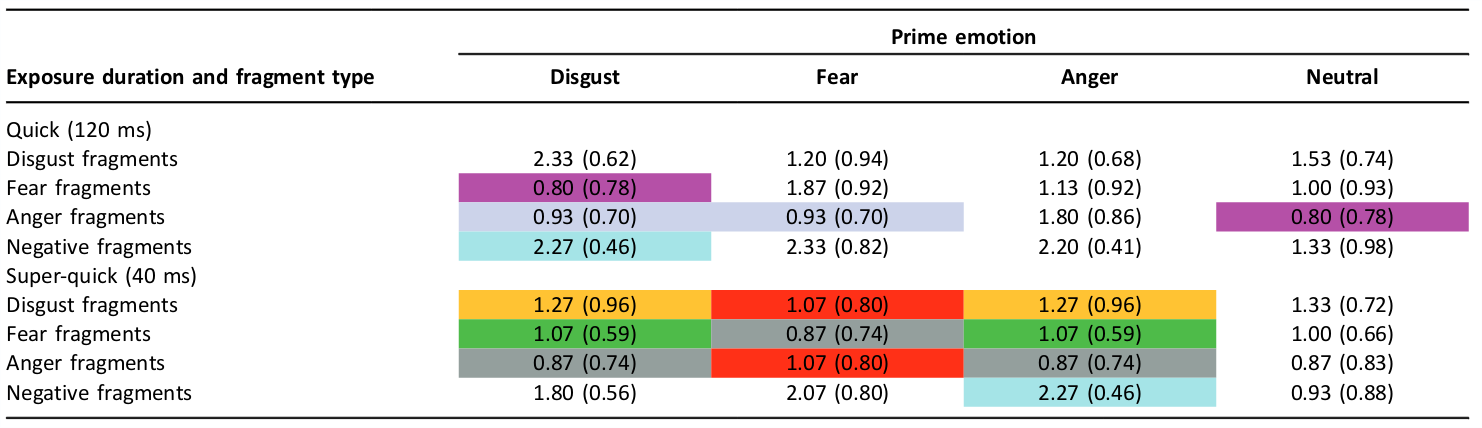
\includegraphics[width=1\linewidth]{assets/figures/scienceopen-table3} 

}

\caption{Reproduction of Table 1 from the retracted Ruys and Stapel (2008) paper. The table shows 32 cells with 'M (SD)', of which 15 are direct duplicates of one of the other cells. The original version with highlighted duplicates can be found at https://osf.io/89mcn.}\label{fig:ruys}
\end{figure}

Why reviewers and editors did not detect this remains a mystery, but it
seems that they simply do not pay attention to potential indicators of
misconduct in the publication process (Bornmann, Nast, and Daniel
\protect\hyperlink{ref-doi:10.1007ux2fs11192-007-1950-2}{2008}). Similar
issues with blatantly problematic results in papers that were later
found to be due to misconduct have been noted in the medical sciences
(Stewart and Feder
\protect\hyperlink{ref-doi:10.1038ux2f325207a0}{1987}). Science has been
regarded as a self-correcting system based on trust. This aligns with
the idea that misconduct occurs because of \enquote{bad apples} (i.e.,
individual factors) and not because of a \enquote{bad barrel} (i.e.,
systemic factors), increasing trust in the scientific enterprise.
However, the self-correcting system has been called a myth (Stroebe,
Postmes, and Spears
\protect\hyperlink{ref-doi:10.1177ux2f1745691612460687}{2012}) and an
assumption that instigates complacency (Hettinger
\protect\hyperlink{ref-doi:10.1038ux2f4661040b}{2010}); if reviewers and
editors have no criteria that pertain to fabrication and falsification
(Bornmann, Nast, and Daniel
\protect\hyperlink{ref-doi:10.1007ux2fs11192-007-1950-2}{2008}), this
implies that the current publication process is not always functioning
properly as a self-correcting mechanism. Moreover, trust in research as
a self-correcting system can be accompanied with complacency by
colleagues in the research process.

The most frequent way data fabrication is detected is by those
researchers who are scrutinous, which ultimately results in
whistleblowing. For example, Stapel's misdeeds were detected by young
researchers who were brave enough to blow the whistle. Although many
regulations include clauses that help protect the whistleblowers,
whistleblowing is known to represent a risk (Lubalin, Ardini, and
Matheson \protect\hyperlink{ref-lubalin1995}{1995}), not only because of
potential backlash but also because the perpetrator is often closely
associated with the whistleblower, potentially leading to negative
career outcomes such as retracted articles on which one is co-author.
This could explain why whistleblowers remain anonymous in only an
estimated 8\% of the cases (Price
\protect\hyperlink{ref-doi:10.1097ux2f00001888-199805000-00009}{1998}).
Negative actions as a result of loss of anonymity include not only
potential loss of a position, but also social and mental health problems
(Lubalin and Matheson
\protect\hyperlink{ref-doi:10.1007ux2fs11948-999-0014-9}{1999}; Allen
and Dowell
\protect\hyperlink{ref-doi:10.1080ux2f08989621.2013.822249}{2013}). It
seems plausible to assume that therefore not all suspicions are
reported.

How often data fabrication and falsification occur is an important
question that can be answered in different ways; it can be approached as
incidence or as prevalence. Incidence refers to new cases in a certain
timeframe, whereas prevalence refers to all cases in the population at a
certain time point. Misconduct cases are often widely publicized, which
might create the image that more cases occur, but the number of cases
seems relatively stable (Rhoades
\protect\hyperlink{ref-rhoades2004}{2004}). Prevalence of research
misconduct is of great interest and, as aforementioned, a meta-analysis
indicated that around 2\% of surveyed researchers admit to fabricating
or falsifying research at least once (Fanelli
\protect\hyperlink{ref-doi:10.1371ux2fjournal.pone.0005738}{2009}).

The prevalence that is of greatest interest is that of how many research
papers contain data that have been fabricated or falsified. Systematic
data on this are unavailable, because papers are not evaluated to this
end in an active manner (Bornmann, Nast, and Daniel
\protect\hyperlink{ref-doi:10.1007ux2fs11192-007-1950-2}{2008}). Only
one case study exists: the Journal of Cell Biology evaluates all
research papers for cell image manipulation (Rossner and Yamada
\protect\hyperlink{ref-doi:10.1083ux2fjcb.200406019}{2004}; Bik,
Casadevall, and Fang
\protect\hyperlink{ref-doi:10.1128ux2fmbio.00809-16}{2016}\protect\hyperlink{ref-doi:10.1128ux2fmbio.00809-16}{a}),
a form of data fabrication/falsification. They have found that
approximately 1\% of all research papers that passed peer review (out of
total of over 3000 submissions) were not published because of the
detection of image manipulation (The Journal of Cell Biology
\protect\hyperlink{ref-cellbio2015}{2015}\protect\hyperlink{ref-cellbio2015}{a}).

\subsection{How can it be prevented?}\label{how-can-it-be-prevented-1}

Notwithstanding discussion about reconciliation of researchers who have
been found guilty of research misconduct (Cressey
\protect\hyperlink{ref-doi:10.1038ux2f493147a}{2013}), these researchers
typically leave science after having been exposed. Hence, improving the
chances of detecting misconduct may help not only in the correction of
the scientific record, but also in the prevention of research
misconduct. In this section we discuss how the detection of fabrication
and falsification might be improved and what to do when misconduct is
detected.

When research is suspect of data fabrication or falsification,
whistleblowers can report these suspicions to institutions, professional
associations, and journals. For example, institutions can launch
investigations via their integrity offices. Typically, a complaint is
submitted to the research integrity officer, who subsequently decides
whether there are sufficient grounds for further investigation. In the
United States, integrity officers have the possibility to sequester,
that is to retrieve, all data of the person in question. If there is
sufficient evidence, a formal misconduct investigation or even a federal
misconduct investigation by the Office of Research Integrity might be
started. Professional associations can also launch some sort of
investigation, if the complaint is made to the association and the
respondent is a member of that association. Journals are also confronted
with complaints about specific research papers and those affiliated with
the Committee on Publication Ethics have a protocol for dealing with
these kinds of allegations (see
\href{https://publicationethics.org/resources}{publicationethics.org/resources}
for details). The best way to improve detection of data fabrication
directly is to further investigate suspicions and report them to your
research integrity office, albeit the potential negative consequences
should be kept in mind when reporting the suspicions, such that it is
best to report anonymously and via analog mail (digital files contain
metadata with identifying information).

More indirectly, statistical tools can be applied to evaluate the
veracity of research papers and raw data (Carlisle et al.
\protect\hyperlink{ref-doi:10.1111ux2fanae.13126}{2015}; Peeters,
Klaassen, and Wiel \protect\hyperlink{ref-peeters2015}{2015}), which
helps detect potential lapses of conduct. Statistical tools have been
successfully applied in data fabrication cases, for instance the Stapel
case (Levelt Committee, Drenth Committee, and Noort, Committee
\protect\hyperlink{ref-levelt2012}{2012}), the Fujii case (Carlisle
\protect\hyperlink{ref-doi:10.1111ux2fj.1365-2044.2012.07128.x}{2012}),
and in the cases of Smeesters and Sanna (Simonsohn
\protect\hyperlink{ref-doi:10.1177ux2f0956797613480366}{2013}).
Interested readers are referred to Buyse et al.
(\protect\hyperlink{ref-buyse1999}{1999}) for a review of statistical
methods to detect potential data fabrication.

Besides using statistics to monitor for potential problems, authors and
principal investigators are responsible for results in the paper and
therefore should invest in verification of results, which improves
earlier detection of problems even if these problems are the result of
mere sloppiness or honest error. Even though it is not feasible for all
authors to verify all results, ideally results should be verified by at
least one co-author. As mentioned earlier, peer-review does not weed out
all major problems (Bornmann, Nast, and Daniel
\protect\hyperlink{ref-doi:10.1007ux2fs11192-007-1950-2}{2008}) and
should not be trusted blindly.

Institutions could facilitate detection of data fabrication and
falsification by implementing data auditing. Data auditing is the
independent verification of research results published in a paper
(Shamoo \protect\hyperlink{ref-doi:10.1038ux2f439784c}{2006}). This goes
hand-in-hand with co-authors verifying results, but this is done by a
researcher not directly affiliated with the research project. Auditing
data is common practice in research that is subject to governmental
oversight, for instance drug trials that are audited by the Food and
Drug Administration (Seife
\protect\hyperlink{ref-doi:10.1001ux2fjamainternmed.2014.7774}{2015}).

Papers that report fabricated or falsified data are typically retracted.
The decision to retract is often (albeit not necessarily) made after the
completion of a formal inquiry and/or investigation of research
misconduct by the academic institution, employer, funding organization
and/or oversight body. Because much of the academic work is done for
hire, the employer can request a retraction from the publisher of the
journal in which the article appeared. Often, the publisher then
consults with the editor (and sometimes also with proprietary
organizations like the professional society that owns the journal title)
to decide on whether to retract. Such processes can be legally complex
if the researcher who was guilty of research misconduct opposes the
retraction. The retraction notice ideally should provide readers with
the main reasons for the retraction, although quite often the notices
lack necessary information (Van Noorden
\protect\hyperlink{ref-doi:10.1038ux2f478026a}{2011}). The popular blog
Retraction Watch normally reports on retractions and often provides
additional information on the reasons for retraction that other parties
involved in the process (co-authors, whistleblowers, the accused
researcher, the (former) employer, and the publisher) are sometimes
reluctant to provide (Marcus and Oransky
\protect\hyperlink{ref-doi:10.1128ux2fjmbe.v15i2.855}{2014}). In some
cases, the editors of a journal may decide to publish an editorial
expression of concern if there are sufficient grounds to doubt the data
in a paper that is being subjected to a formal investigation of research
misconduct.

Many retracted articles are still cited after the retraction has been
issued (Bornemann-Cimenti, Szilagyi, and Sandner-Kiesling
\protect\hyperlink{ref-doi:10.1007ux2fs11948-015-9680-y}{2015}; Pfeifer
and Snodgrass
\protect\hyperlink{ref-doi:10.1001ux2fjama.1990.03440100140020}{1990}).
Additionally, retractions might be issued following a misconduct
investigation, but not completed by journals, that the original content
is simply deleted, or that legal threats resulted in not retracting the
work (Elia, Wager, and Tramèr
\protect\hyperlink{ref-doi:10.1371ux2fjournal.pone.0085846}{2014}). If
retractions do not occur even though they have been issued, their
negative effect, for instance decreased author citations (Lu et al.
\protect\hyperlink{ref-doi:10.1038ux2fsrep03146}{2013}), are nullified,
reducing the costs of committing misconduct.

\section{Conclusion}\label{conclusion}

This chapter provides an overview of the research practice spectrum,
where on the one end there is
\protect\hyperlink{responsible-conduct-of-research}{responsible conduct
of research} and with \protect\hyperlink{research-misconduct}{research
misconduct} on the other end. In sum, transparent research practices are
proposed to embody scientific norms and a way to deal with both
questionable research practices and research misconduct,
\protect\hyperlink{improving-responsible-conduct}{inducing better
research practices}. This would improve not only the documentation and
verification of research results; it also helps create a more open
environment for researchers to actively discuss ethical problems and
handle problems in a responsible manner, promoting good research
practices. This might help reduce both questionable research practices
and research misconduct.

\chapter{\texorpdfstring{Reanalyzing Head et al. (2015): investigating
the robustness of widespread
\(p\)-hacking}{Reanalyzing Head et al. (2015): investigating the robustness of widespread p-hacking}}\label{reanalyzing-head-et-al.-2015-investigating-the-robustness-of-widespread-p-hacking}

Head et al.
(\protect\hyperlink{ref-doi:10.1371ux2fjournal.pbio.1002106}{2015}\protect\hyperlink{ref-doi:10.1371ux2fjournal.pbio.1002106}{b})
provided a large collection of \(p\)-values that, from their
perspective, indicates widespread statistical significance seeking
(i.e., \(p\)-hacking) throughout the sciences. This result has been
questioned from an epistemological perspective because analyzing all
reported \(p\)-values in research articles answers the supposedly
inappropriate question of evidential value across all results
(Simonsohn, Simmons, and Nelson
\protect\hyperlink{ref-doi:10.1037ux2fxge0000104}{2015}). Adjacent to
epistemological concerns, the robustness of widespread \(p\)-hacking in
these data can be questioned due to the large variation in a priori
choices with regards to data analysis. Head et al.
(\protect\hyperlink{ref-doi:10.1371ux2fjournal.pbio.1002106}{2015}\protect\hyperlink{ref-doi:10.1371ux2fjournal.pbio.1002106}{b})
had to make several decisions with respect to the data analysis, which
might have affected the results. In this chapter I evaluate the data
analysis approach with which Head et al.
(\protect\hyperlink{ref-doi:10.1371ux2fjournal.pbio.1002106}{2015}\protect\hyperlink{ref-doi:10.1371ux2fjournal.pbio.1002106}{b})
found widespread \(p\)-hacking and propose that this effect is not
robust to several justifiable changes. The underlying models for their
findings have been discussed in several preprints (e.g., Bishop and
Thompson
\protect\hyperlink{ref-doi:10.7287ux2fpeerj.preprints.1266v1}{2015};
Holman
\protect\hyperlink{ref-doi:10.6084ux2fm9.figshare.1500901.v1}{2015}) and
publications (e.g., Simonsohn, Simmons, and Nelson
\protect\hyperlink{ref-doi:10.1037ux2fxge0000104}{2015}; Bruns and
Ioannidis
\protect\hyperlink{ref-doi:10.1371ux2fjournal.pone.0149144}{2016}), but
the data have not extensively been reanalyzed for robustness.

The \(p\)-value distribution of a set of true- and null results without
\(p\)-hacking should be a mixture distribution of only the uniform
\(p\)-value distribution under the null hypothesis \(H_0\) and
right-skew \(p\)-value distributions under the alternative hypothesis
\(H_1\). \(P\)-hacking behaviors affect the distribution of
statistically significant \(p\)-values, potentially resulting in
left-skew below .05 (i.e., a bump), but not necessarily so (Hartgerink
et al. \protect\hyperlink{ref-doi:10.7717ux2fpeerj.1935}{2016}; Lakens
\protect\hyperlink{ref-doi:10.1080ux2f17470218.2014.982664}{2015}\protect\hyperlink{ref-doi:10.1080ux2f17470218.2014.982664}{a};
Bishop and Thompson
\protect\hyperlink{ref-doi:10.7717ux2fpeerj.1715}{2016}). An example of
a questionable behavior that can result in left-skew is optional
stopping (i.e., data peeking) if the null hypothesis is true (Lakens
\protect\hyperlink{ref-doi:10.1080ux2f17470218.2014.982664}{2015}\protect\hyperlink{ref-doi:10.1080ux2f17470218.2014.982664}{a}).

Consequently, Head et al.
(\protect\hyperlink{ref-doi:10.1371ux2fjournal.pbio.1002106}{2015}\protect\hyperlink{ref-doi:10.1371ux2fjournal.pbio.1002106}{b})
correctly argue that an aggregate \(p\)-value distribution could show a
bump below .05 when left-skew \(p\)-hacking occurs frequently.
Questionable behaviors that result in seeking statistically significant
results, such as (but not limited to) the aforementioned optional
stopping under \(H_0\), could result in a bump below .05. Hence, a
systematic bump below .05 (i.e., not due to sampling error) is a
sufficient condition for the presence of specific forms of
\(p\)-hacking. However, this bump below .05 is not a necessary
condition, because other types of \(p\)-hacking can still occur without
a bump below .05 presenting itself (Hartgerink et al.
\protect\hyperlink{ref-doi:10.7717ux2fpeerj.1935}{2016}; Lakens
\protect\hyperlink{ref-doi:10.1080ux2f17470218.2014.982664}{2015}\protect\hyperlink{ref-doi:10.1080ux2f17470218.2014.982664}{a};
Bishop and Thompson
\protect\hyperlink{ref-doi:10.7717ux2fpeerj.1715}{2016}). For example,
one might use optional stopping when there is a true effect or conduct
multiple analyses, but only report that statistical test which yielded
the smallest \(p\)-value. Therefore, if no bump of statistically
significant \(p\)-values is found, this does not exclude that
\(p\)-hacking occurs at a large scale.

In the current chapter, the conclusion from Head et al.
(\protect\hyperlink{ref-doi:10.1371ux2fjournal.pbio.1002106}{2015}\protect\hyperlink{ref-doi:10.1371ux2fjournal.pbio.1002106}{b})
is inspected for robustness. Their conclusion is that the data fullfill
the sufficient condition for \(p\)-hacking (i.e., show a systematic bump
below .05), hence, provides evidence for the presence of specific forms
of \(p\)-hacking. The robustness of this conclusion is inspected in
three steps: (i) explaining the data and data analysis strategies
(original and reanalysis), (ii) reevaluating the evidence for a bump
below .05 (i.e., the sufficient condition) based on the reanalysis, and
(iii) discussing whether this means that there is no widespread
\(p\)-hacking in the literature.

\section{Data and methods}\label{data-and-methods}

In the original paper, over two million reported \(p\)-values were mined
from the \href{https://www.ncbi.nlm.nih.gov/pmc/tools/openftlist/}{Open
Access subset of PubMed central}. PubMed central indexes the biomedical
and life sciences and permits bulk downloading of full-text Open Access
articles. By text-mining these full-text articles for \(p\)-values, Head
et al.
(\protect\hyperlink{ref-doi:10.1371ux2fjournal.pbio.1002106}{2015}\protect\hyperlink{ref-doi:10.1371ux2fjournal.pbio.1002106}{b})
extracted more than two million \(p\)-values in total. Their text-mining
procedure extracted all reported \(p\)-values, including those that were
reported without an accompanying test statistic. For example, the
\(p\)-value from the result \(t(59)=1.75,p>.05\) was included, but also
a lone \(p<.05\). Subsequently, Head et al.
(\protect\hyperlink{ref-doi:10.1371ux2fjournal.pbio.1002106}{2015}\protect\hyperlink{ref-doi:10.1371ux2fjournal.pbio.1002106}{b})
analyzed a subset of statistically significant \(p\)-values (assuming
\(\alpha=.05\)) that were exactly reported (e.g., \(p=.043\); the same
subset is analyzed in this chapter).

Head et al.
(\protect\hyperlink{ref-doi:10.1371ux2fjournal.pbio.1002106}{2015}\protect\hyperlink{ref-doi:10.1371ux2fjournal.pbio.1002106}{b})
their data analysis approach focused on comparing frequencies in the
last and penultimate bins from .05 at a binwidth of .005 (i.e.,
\(.04<p< .045\) versus \(.045<p<.05\)). Based on the tenet that a
sufficient condition for \(p\)-hacking is a systematic bump of
\(p\)-values below .05 (Simonsohn, Nelson, and Simmons
\protect\hyperlink{ref-doi:10.1037ux2fa0033242}{2014}), sufficient
evidence for \(p\)-hacking is present if the last bin has a
significantly higher frequency than the penultimate bin in a binomial
test. Applying the binomial test (i.e., Caliper test) to two frequency
bins has previously been used in publication bias research (Gerber et
al. \protect\hyperlink{ref-doi:10.1177ux2f1532673x09350979}{2010};
Kühberger, Fritz, and Scherndl
\protect\hyperlink{ref-doi:10.1371ux2fjournal.pone.0105825}{2014}),
applied here specifically to test for \(p\)-hacking behaviors that
result in a bump below .05. The binwidth of .005 and the bins
\(.04<p<.045\) and \(.045<p<.05\) were chosen by Head et al.
(\protect\hyperlink{ref-doi:10.1371ux2fjournal.pbio.1002106}{2015}\protect\hyperlink{ref-doi:10.1371ux2fjournal.pbio.1002106}{b})
because they expected the signal of this form of \(p\)-hacking to be
strongest in this part of the distribution (regions of the \(p\)-value
distribution closer to zero are more likely to contain evidence of true
effects than regions close to .05). They excluded \(p=.05\)
\enquote{because {[}they{]} suspect{[}ed{]} that many authors do not
regard \(p=0.05\) as significant} (p.4).

\begin{figure}

{\centering 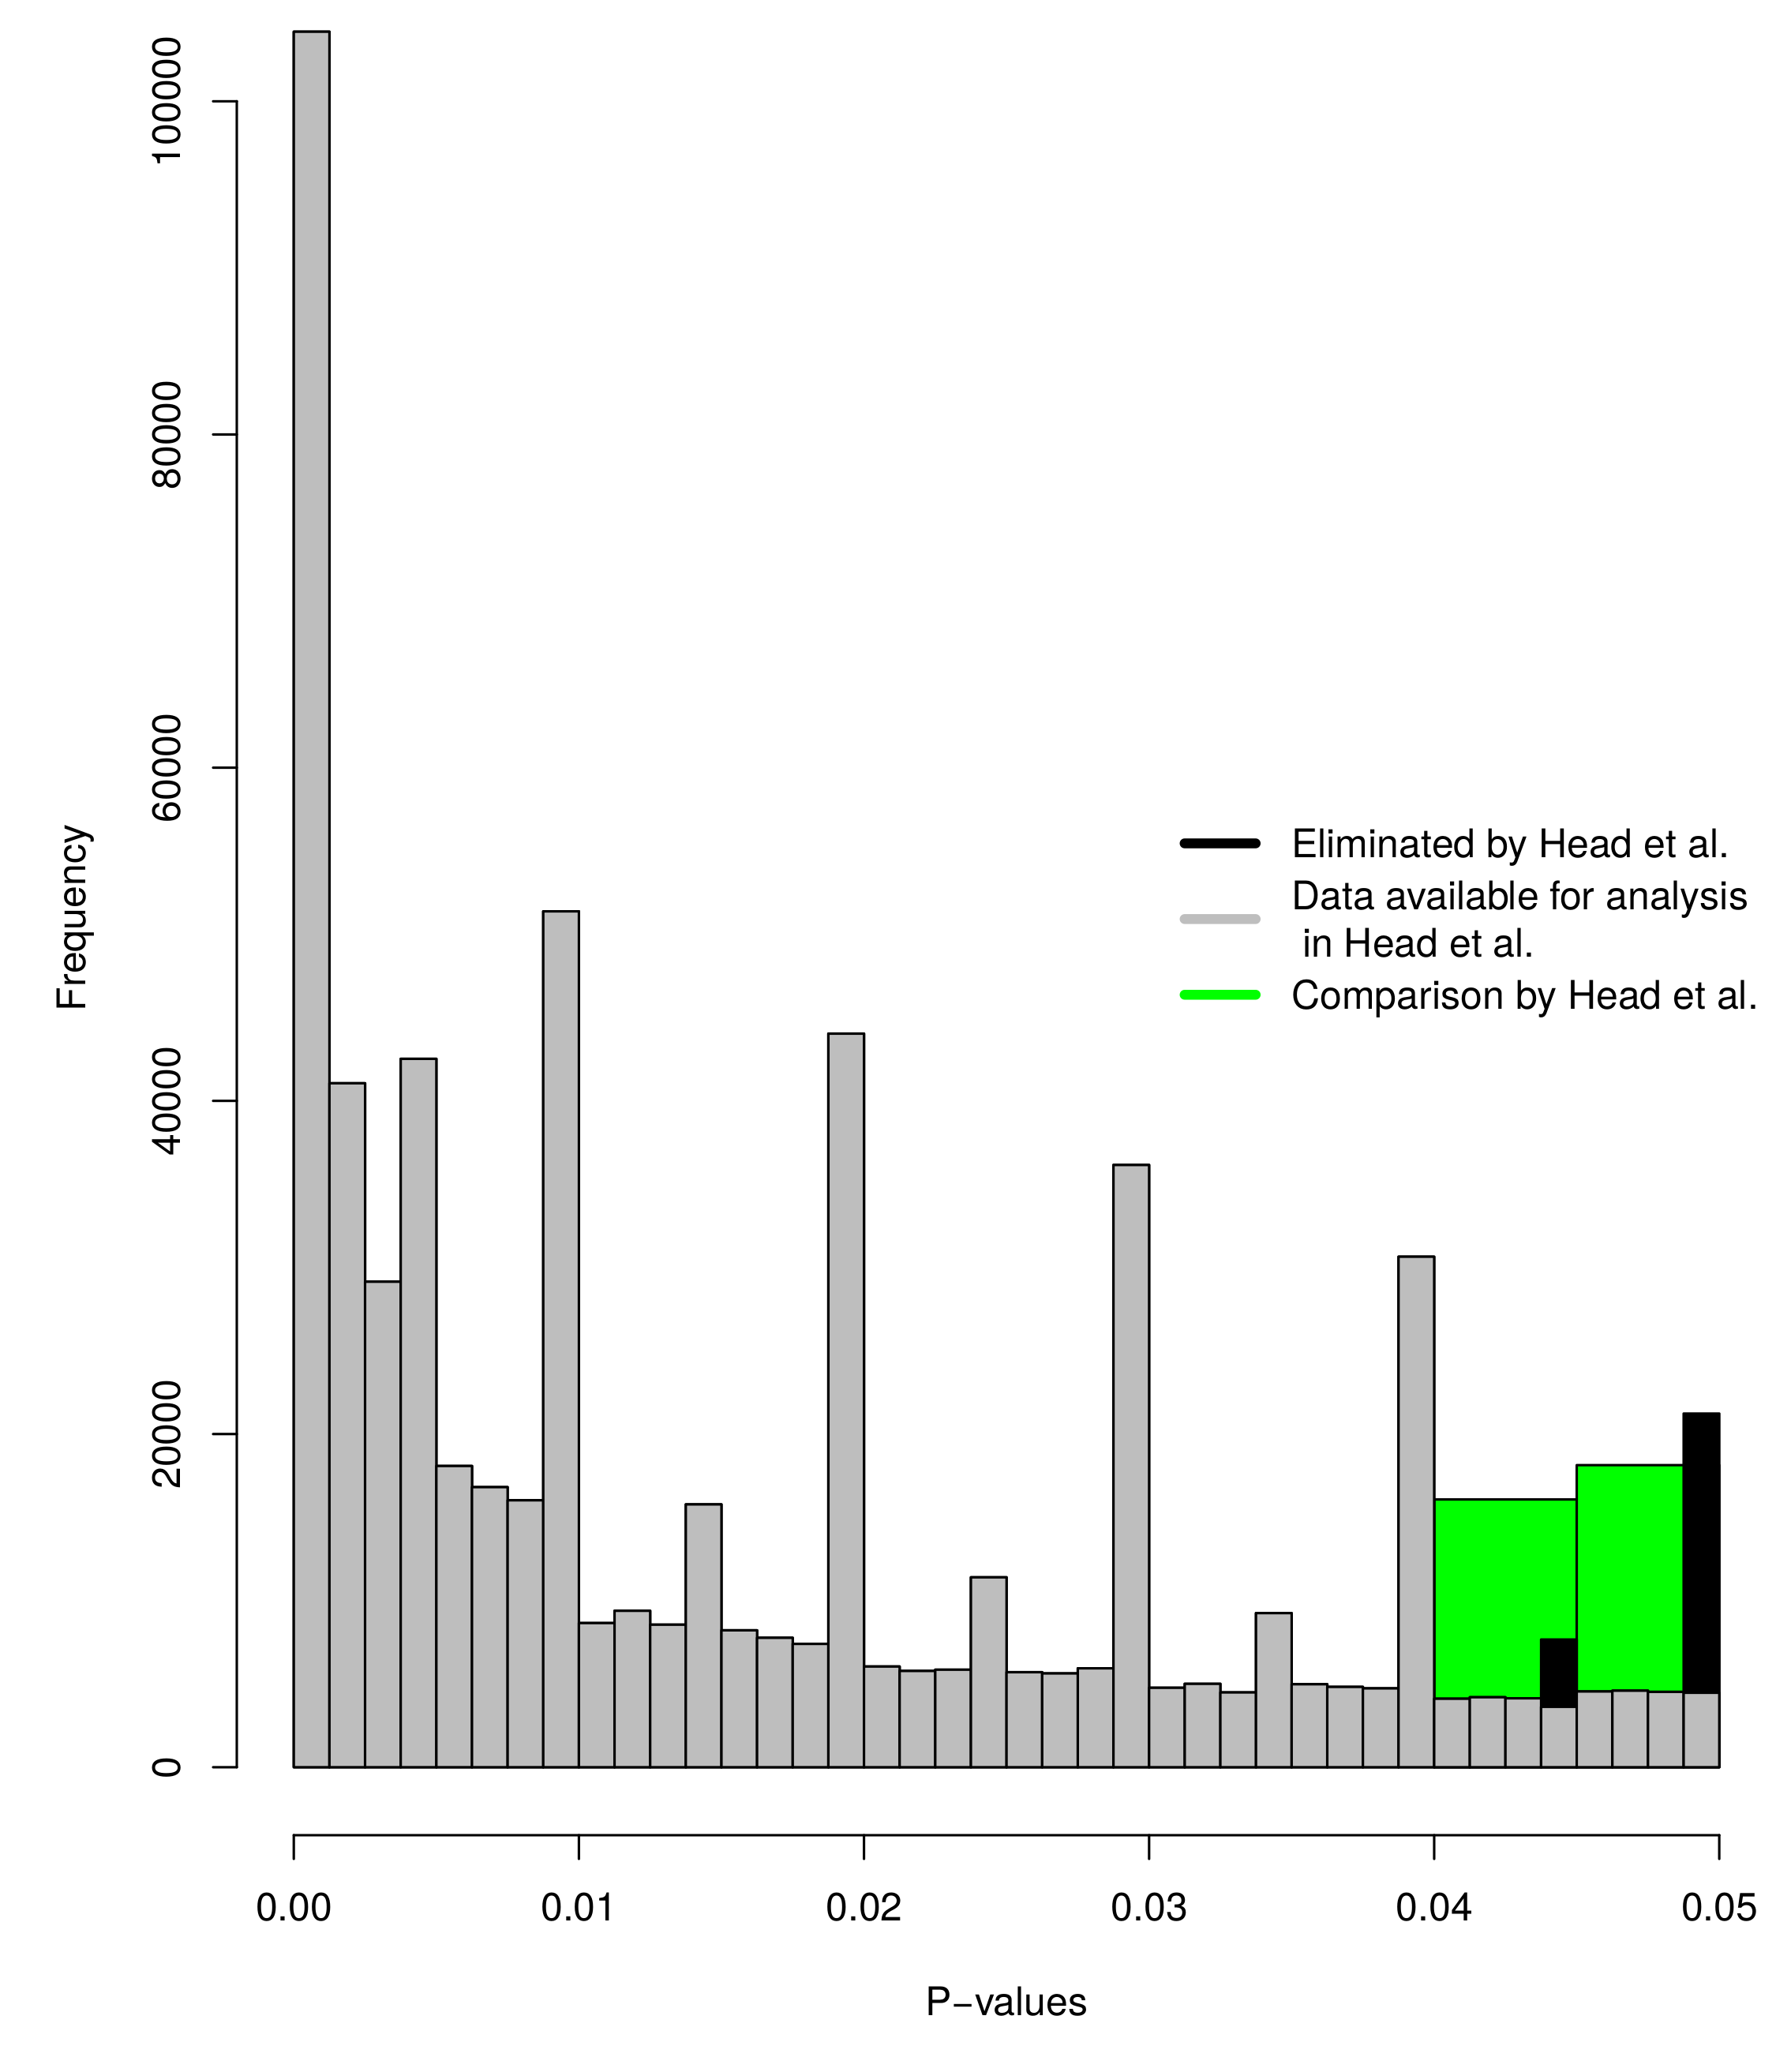
\includegraphics[width=0.8\linewidth]{assets/figures/head-fig1} 

}

\caption{Histograms of p-values as selected in Head et al. (in green; $.04 < p < .045$ versus $.045 < p < .05$), the significant $p$-value distribution as selected in Head et al. (in grey; $0<p\leq.00125$, $.00125<p\leq.0025$, ..., $.0475<p\leq.04875$, $.04875<p<.05$, binwidth = .00125). The green and grey histograms exclude $p=.045$ and $p=.05$; the black histogram shows the frequencies of results that are omitted because of this ($.04375<p\leq.045$ and $.04875<p\leq.05$, binwidth = .00125).}\label{fig:head-hist}
\end{figure}

Figure \ref{fig:head-hist} shows the selection of \(p\)-values in Head
et al.
(\protect\hyperlink{ref-doi:10.1371ux2fjournal.pbio.1002106}{2015}\protect\hyperlink{ref-doi:10.1371ux2fjournal.pbio.1002106}{b})
in two ways: (1) in green, which shows the results as analysed by Head
et al. (i.e., \(.04<p<.045\) versus \(.045<p<.05\)), and (2) in grey,
which shows the entire distribution of significant \(p\)-values
(assuming \(\alpha=.05\)) available to Head et al. after eliminating
\(p=.045\) and \(p=.05\) (depicted by the black bins). The height of the
two green bins (i.e., the sum of the grey bins in the same range) show a
bump below .05, which indicates \(p\)-hacking. The grey histogram in
Figure \ref{fig:head-hist} shows a more fine-grained depiction of the
\(p\)-value distribution and does not clearly show a bump below .05,
because it is dependent on which bins are compared. However, the grey
histogram clearly indicates that results around the second decimal tend
to be reported more frequently when \(p\geq.01\).

Theoretically, the \(p\)-value distribution should be a smooth,
decreasing function, but the grey distribution shows systematically more
reported \(p\)-values for .01, .02, .03, .04 (and .05 when the black
histogram is included). As such, there seems to be a tendency to report
\(p\)-values to two decimal places, instead of three. For example,
\(p=.041\) might be correctly rounded down to \(p=.04\) or \(p=.046\)
rounded up to \(p=.05\). A potential post-hoc explanation is that three
decimal reporting of \(p\)-values is a relatively recent standard, if a
standard at all. For example, it has only been prescribed since 2010 in
psychology (American Psychological Association
\protect\hyperlink{ref-isbn:9781433805615}{2010}\protect\hyperlink{ref-isbn:9781433805615}{b}),
where it previously prescribed two decimal reporting (American
Psychological Association
\protect\hyperlink{ref-American_Psychological_Association1983-yf}{1983};
American Psychological Association
\protect\hyperlink{ref-American_Psychological_Association2001-uw}{2001}).
Given the results, it seems reasonable to assume that other fields might
also report to two decimal places instead of three, most of the time.

Moreover, the data analysis approach used by Head et al.
(\protect\hyperlink{ref-doi:10.1371ux2fjournal.pbio.1002106}{2015}\protect\hyperlink{ref-doi:10.1371ux2fjournal.pbio.1002106}{b})
eliminates \(p=.045\) for symmetry of the compared bins and \(p=.05\)
based on a potentially invalid assumption of when researchers regard
results as statistically significant. \(P=.045\) is not included in the
selected bins (\(.04<p<.045\) versus \(.045<p<.05\)), while this could
affect the results. If \(p=.045\) is included, no evidence of a bump
below .05 is found (the left black bin in Figure \ref{fig:head-hist} is
then included; frequency \(.04<p\leq.045=20114\) versus
\(.045<p<.05=18132\)). However, the bins are subsequently asymmetrical
and require a different analysis. To this end, I supplement the Caliper
tests with Fisher's method (Fisher
\protect\hyperlink{ref-Fisher1925-jl}{1925}; Mosteller and Fisher
\protect\hyperlink{ref-doi:10.2307ux2f2681650}{1948}) based on the same
range analyzed by Head et al.
(\protect\hyperlink{ref-doi:10.1371ux2fjournal.pbio.1002106}{2015}\protect\hyperlink{ref-doi:10.1371ux2fjournal.pbio.1002106}{b}).
This analysis includes \(.04<p<.05\) (i.e., it does not exclude
\(p=.045\) as in the binned Caliper test). Fisher's method tests for a
deviation from uniformity and was computed as

\begin{equation} 
  \chi^2_{2k}=-2\sum^k_{i=1}ln(\frac{p_i-.04}{.01})
  \label{eq:fishmeth}
\end{equation}

where \(p_i\) are the \(p\)-values between \(.04<p<.05\). Effectively,
Equation \eqref{eq:fishmeth} tests for a bump between .04 and .05 (i.e.,
the transformation ensures that the transformed \(p\)-values range from
0-1 and that Fisher's method inspects left-skew instead of right-skew).
\(P=.05\) was consistently excluded by Head et al.
(\protect\hyperlink{ref-doi:10.1371ux2fjournal.pbio.1002106}{2015}\protect\hyperlink{ref-doi:10.1371ux2fjournal.pbio.1002106}{b})
because they assumed researchers did not interpret this as statistically
significant. However, researchers interpret \(p=.05\) as statistically
significant more frequently than they thought: 94\% of 236 cases
investigated by Nuijten, Hartgerink, et al.
(\protect\hyperlink{ref-doi:10.3758ux2fs13428-015-0664-2}{2015})
interpreted \(p=.05\) as statistically significant, indicating this
assumption might not be valid.

Given that systematically more \(p\)-values are reported to two decimal
places and the adjustments described in the previous paragraph, I did
not exclude \(p=.045\) and \(p=.05\) and I adjusted the bin selection to
\(.03875<p\leq.04\) versus \(.04875<p\leq.05\). Visually, the newly
selected data are the grey and black bins from Figure
\ref{fig:head-hist} combined, where the rightmost black bin (i.e.,
\(.04875<p\leq.05\)) is compared with the large grey bin at .04 (i.e.,
\(.03875<p\leq.04\)). The bins \(.03875<p\leq.04\) and
\(.04875<p\leq.05\) were selected to take into account that \(p\)-values
are typically rounded (both up and down) in the observed data. Moreover,
if incorrect or excessive rounding-down of \(p\)-values occurs
strategically (e.g., \(p=.054\) reported as \(p=.05\); Vermeulen et al.
\protect\hyperlink{ref-doi:10.1080ux2f19312458.2015.1096333}{2015}),
this can be considered \(p\)-hacking. If \(p=.05\) is excluded from the
analyses, these types of \(p\)-hacking behaviors are eliminated from the
analyses, potentially decreasing the sensitivity of the test for a bump.

The reanalysis approach for the bins \(.03875<p\leq.04\) and
\(.04875<p\leq.05\) is similar to Head et al.
(\protect\hyperlink{ref-doi:10.1371ux2fjournal.pbio.1002106}{2015}\protect\hyperlink{ref-doi:10.1371ux2fjournal.pbio.1002106}{b})
and applies the Caliper test to detect a bump below .05, with the
addition of Bayesian Caliper tests. The Caliper test investigates
whether the bins are equally distributed or that the penultimate bin
(i.e., \(.03875<p\leq.04\)) contains more results than the ultimate bin
(i.e., \(.04875<p\leq.05\); \(H_0:Proportion\leq.5\)). Sensitivity
analyses were also conducted, altering the binwidth from .00125 to .005
and .01. Moreover, the analyses were conducted for both the \(p\)-values
extracted from the abstracts- and the results sections separately.

The results from the Bayesian Caliper test and the traditional,
frequentist Caliper test give results with different interpretations.
The \(p\)-value of the Caliper test gives the probability of more
extreme results if the null hypothesis is true, but does not quantify
the probability of the null- and alternative hypothesis. The added value
of the Bayes Factor (\(BF\)) is that it does quantify the probabilities
of the hypotheses in the model and creates a ratio, either as
\(BF_{10}\), the alternative hypothesis versus the null hypothesis, or
vice versa, \(BF_{01}\). A \(BF\) of 1 indicates that both hypotheses
are equally probable, given the data. All Bayesian proportion tests were
conducted with highly uncertain priors (\(r=1\), \enquote{ultrawide}
prior) using the \texttt{BayesFactor} package (Morey and Rouder
\protect\hyperlink{ref-bf}{2015}). In this specific instance,
\(BF_{10}\) is computed and values \(>1\) can be interpreted, for our
purposes, as: the data are more likely under \(p\)-hacking that results
in a bump below .05 (i.e., left-skew \(p\)-hacking) than under no
left-skew \(p\)-hacking. \(BF_{10}\) values \(<1\) indicate that the
data are more likely under no left-skew \(p\)-hacking than under
left-skew \(p\)-hacking. The further removed from \(1\), the more
evidence in the direction of either hypothesis is available.

\section{Reanalysis results}\label{reanalysis-results}

Results of Fisher's method for all \(p\)-values between \(.04<p<.05\)
and does not exclude \(p=.045\) fails to find evidence for a bump below
.05, \(\chi^2(76492)=70328.86,p>.999\). Additionally, no evidence for a
bump below .05 remains when I focus on the more frequently reported
second-decimal bins, which could include \(p\)-hacking behaviors such as
incorrect or excessive rounding down to \(p=.05\). Reanalyses showed no
evidence for left-skew \(p\)-hacking,
\(Proportion=.417,p>.999, BF_{10}<.001\) for the Results sections and
\(Proportion=.358,p>.999,BF_{10}<.001\) for the Abstract sections. Table
\ref{tab:caliper-table} summarizes these results for alternate binwidths
(.00125, .005, and .01) and shows results are consistent across
different binwidths. Separated per discipline, no binomial test for
left-skew \(p\)-hacking is statistically significant in either the
Results- or Abstract sections (see the Supporting Information). This
indicates that the evidence for \(p\)-hacking that results in a bump
below .05, as presented by Head et al.
(\protect\hyperlink{ref-doi:10.1371ux2fjournal.pbio.1002106}{2015}\protect\hyperlink{ref-doi:10.1371ux2fjournal.pbio.1002106}{b}),
seems to not be robust to minor changes in the analysis such as
including \(p=.045\) by evaluating \(.04<p<.05\) continuously instead of
binning, or when taking into account the observed tendency to round
\(p\)-values to two decimal places during the bin selection.

\begin{table}[!h]

\caption{\label{tab:caliper-table}Results of the reanalysis across various binwidths (i.e., .00125, .005, .01) and different sections of the paper.}
\centering
\begin{tabular}{llll}
\toprule
 &  & Abstracts & Results\\
\midrule
\rowcolor{gray!6}  Binwidth = .00125 & $.03875 < p \leq .04$ & 4597 & 26047\\
 & $.04875 < p \leq .05$ & 2565 & 18664\\
\rowcolor{gray!6}   & Proportion & 0.358 & 0.417\\
 & $p$ & $>.999$ & \vphantom{2} $>.999$\\
\rowcolor{gray!6}   & $BF_{10}$ & $<.001$ & \vphantom{2} $<.001$\\
\addlinespace
Binwidth = .005 & $.035 < p \leq .04$ & 6641 & 38537\\
\rowcolor{gray!6}   & $.045 < p \leq .05$ & 4485 & 30406\\
 & Proportion & 0.403 & 0.441\\
\rowcolor{gray!6}   & $p$ & $>.999$ & \vphantom{1} $>.999$\\
 & $BF_{10}$ & $<.001$ & \vphantom{1} $<.001$\\
\addlinespace
\rowcolor{gray!6}  Binwidth = .01 & $.03 < p \leq .04$ & 9885 & 58809\\
 & $.04 < p \leq .05$ & 7250 & 47755\\
\rowcolor{gray!6}   & Proportion & 0.423 & 0.448\\
 & $p$ & $>.999$ & $>.999$\\
\rowcolor{gray!6}   & $BF_{10}$ & $<.001$ & $<.001$\\
\bottomrule
\end{tabular}
\end{table}

\section{Discussion}\label{discussion}

Head et al.
(\protect\hyperlink{ref-doi:10.1371ux2fjournal.pbio.1002106}{2015}\protect\hyperlink{ref-doi:10.1371ux2fjournal.pbio.1002106}{b})
collected \(p\)-values from full-text articles and analyzed these for
\(p\)-hacking, concluding that \enquote{\(p\)-hacking is widespread
throughout science} (see abstract; Head et al.
\protect\hyperlink{ref-doi:10.1371ux2fjournal.pbio.1002106}{2015}\protect\hyperlink{ref-doi:10.1371ux2fjournal.pbio.1002106}{b}).
Given the implications of such a finding, I inspected whether evidence
for widespread \(p\)-hacking was robust to some substantively justified
changes in the data selection. A minor adjustment from comparing bins to
continuously evaluating \(.04<p<.05\), the latter not excluding .045,
already indicated this finding seems to not be robust. Additionally,
after altering the bins inspected due to the observation that
systematically more \(p\)-values are reported to the second decimal and
including \(p=.05\) in the analyses, the results indicate that evidence
for widespread \(p\)-hacking, as presented by Head et al.
(\protect\hyperlink{ref-doi:10.1371ux2fjournal.pbio.1002106}{2015}\protect\hyperlink{ref-doi:10.1371ux2fjournal.pbio.1002106}{b})
is not robust to these substantive changes in the analysis. Moreover,
the frequency of \(p=.05\) is directly affected by \(p\)-hacking, when
rounding-down of \(p\)-values is done strategically. The conclusion
drawn by Head et al.
(\protect\hyperlink{ref-doi:10.1371ux2fjournal.pbio.1002106}{2015}\protect\hyperlink{ref-doi:10.1371ux2fjournal.pbio.1002106}{b})
might still be correct, but the data do not undisputably show so.
Moreover, even if there is no \(p\)-hacking that results in a bump of
\(p\)-values below .05, other forms of \(p\)-hacking that do not cause
such a bump can still be present and prevalent (Hartgerink et al.
\protect\hyperlink{ref-doi:10.7717ux2fpeerj.1935}{2016}; Lakens
\protect\hyperlink{ref-doi:10.1080ux2f17470218.2014.982664}{2015}\protect\hyperlink{ref-doi:10.1080ux2f17470218.2014.982664}{a};
Bishop and Thompson
\protect\hyperlink{ref-doi:10.7717ux2fpeerj.1715}{2016}).

Second-decimal reporting tendencies of \(p\)-values should be taken into
consideration when selecting bins for inspection because this dataset
does not allow for the elimination of such reporting tendencies. Its
substantive consequences are clearly depicted in the results of the
reanalysis and Figure \ref{fig:head-hist} illustrates how the
theoretical properties of \(p\)-value distributions do not hold for the
reported \(p\)-value distribution. Previous research has indicated that
when the recalculated \(p\)-value distribution is inspected, the
theoretically expected smooth distribution re-emerges even when the
reported \(p\)-value distribution shows reporting tendencies (Hartgerink
et al. \protect\hyperlink{ref-doi:10.7717ux2fpeerj.1935}{2016}; Krawczyk
\protect\hyperlink{ref-doi:10.1371ux2fjournal.pone.0127872}{2015}).
Given that the text-mining procedure implemented by Head et al.
(\protect\hyperlink{ref-doi:10.1371ux2fjournal.pbio.1002106}{2015}\protect\hyperlink{ref-doi:10.1371ux2fjournal.pbio.1002106}{b})
does not allow for recalculation of \(p\)-values, the effect of
reporting tendencies needs to mitigated by altering the data analysis
approach.

Even after mitigating the effect of reporting tendencies, these analyses
were all conducted on a set of aggregated \(p\)-values, which can either
detect \(p\)-hacking that results in a bump of \(p\)-values below .05 if
it is widespread, but not prove that no \(p\)-hacking is going on in any
of the individual papers. Firstly, there is the risk of an ecological
fallacy. These analyses take place at the aggregate level, but there
might still be research papers that show a bump below .05 at the paper
level. Secondly, some forms of \(p\)-hacking also result in right-skew,
which is not picked up in these analyses and is difficult to detect in a
set of heterogeneous results (attempted in Hartgerink et al.
\protect\hyperlink{ref-doi:10.7717ux2fpeerj.1935}{2016}). As such, if
any detection of \(p\)-hacking is attempted, this should be done at the
paper level and after careful scrutiny of which results are included
(Simonsohn, Simmons, and Nelson
\protect\hyperlink{ref-doi:10.1037ux2fxge0000104}{2015}; Bishop and
Thompson \protect\hyperlink{ref-doi:10.7717ux2fpeerj.1715}{2016}).

\section{Limitations and conclusion}\label{limitations-and-conclusion}

In this reanalysis two limitations remain with respect to the data
analysis. First, selecting the bins just below .04 and .05 results in
selecting non-adjacent bins. Hence, the test might be less sensitive to
detect a bump below .05. In light of this limitation I ran the original
analysis from Head et al.
(\protect\hyperlink{ref-doi:10.1371ux2fjournal.pbio.1002106}{2015}\protect\hyperlink{ref-doi:10.1371ux2fjournal.pbio.1002106}{b}),
but included the second decimal (i.e., \(.04\leq p<.045\) versus
\(.045<p\leq.05\)). This analysis also yielded no evidence for a bump of
\(p\)-values below .05, \(Proportion=.431,p>.999,BF_{10}<.001\). Second,
the selection of only exactly reported \(p\)-values might have distorted
the \(p\)-value distribution due to reporting tendencies in rounding.
For example, a researcher with a \(p\)-value of .047 might be more
likely to report \(p<.05\) than a researcher with a \(p\)-value of .037
reporting \(p<.04\). Given that these analyses exclude all values
reported as \(p<X\), this could have affected the results. There is some
indication that this tendency to round up is relatively stronger around
.05 than around .04 (a factor of 1.25 approximately based on the
\href{https://doi.org/10.1371/journal.pone.0127872.g005}{original Figure
5}; Krawczyk
\protect\hyperlink{ref-doi:10.1371ux2fjournal.pone.0127872}{2015}),
which might result in an underrepresentation of \(p\)-values around .05.

Given the implications of the findings by Head et al.
(\protect\hyperlink{ref-doi:10.1371ux2fjournal.pbio.1002106}{2015}\protect\hyperlink{ref-doi:10.1371ux2fjournal.pbio.1002106}{b}),
it is important that these findings are robust to choices that can vary.
Moreover, the absence of a bump below .05 seems to be stronger than its
presence throughout the literature: a reanalysis of a previous paper,
which found evidence for a bump below .05 (Masicampo and Lalande
\protect\hyperlink{ref-doi:10.1080ux2f17470218.2012.711335}{2012}),
yielded no evidence for a bump below .05 (Lakens
\protect\hyperlink{ref-doi:10.1080ux2f17470218.2014.982664}{2015}\protect\hyperlink{ref-doi:10.1080ux2f17470218.2014.982664}{a});
two new datasets also did not reveal a bump below .05 (Hartgerink et al.
\protect\hyperlink{ref-doi:10.7717ux2fpeerj.1935}{2016}; Vermeulen et
al. \protect\hyperlink{ref-doi:10.1080ux2f19312458.2015.1096333}{2015}).
Consequently, findings that claim there is a bump below .05 need to be
robust. In this chapter, I explained why a different data analysis
approach to the data of Head et al.
(\protect\hyperlink{ref-doi:10.1371ux2fjournal.pbio.1002106}{2015}\protect\hyperlink{ref-doi:10.1371ux2fjournal.pbio.1002106}{b})
can be justified and as a result no evidence of widespread \(p\)-hacking
that results in a bump of \(p\)-values below .05 is found. Although this
does not mean that no \(p\)-hacking occurs at all, the conclusion by
Head et al.
(\protect\hyperlink{ref-doi:10.1371ux2fjournal.pbio.1002106}{2015}\protect\hyperlink{ref-doi:10.1371ux2fjournal.pbio.1002106}{b})
should not be taken at face value considering that the results are not
robust to (minor) choices in the data analysis approach. As such, the
evidence for widespread left-skew \(p\)-hacking is ambiguous at best.

\section{Supporting Information}\label{supporting-information}

S1 File. Full reanalysis results per discipline:
\url{https://doi.org/10.7717/peerj.3068/supp-1}.

\chapter{Distributions of p-values between .01-.05 in psychology: what
is going
on?}\label{distributions-of-p-values-between-.01-.05-in-psychology-what-is-going-on}

A set of \(p\)-values can be informative of the underlying effects that
are investigated, but can also be indicative of potential research
biases or questionable research practices (QRPs). In the absence of
QRPs, the distribution of significant \(p\)-values can be expected to
have a certain shape. Under the null-hypothesis all \(p\)-values are
equally probable (i.e., follow a uniform distribution). If there is
truly an effect, smaller \(p\)-values are more likely than larger
\(p\)-values (i.e., the distribution decreases monotonically in the
\(p\)-value). Consequently, because some hypotheses are false and some
are true, the distribution of observed \(p\)-values arises from a
mixture of uniform and right-skewed distributions and should also
decrease monotonically.\footnote{One exception to this rule is when the
  alternative hypothesis is wrongly specified, that is, if the true
  effect size is negative whereas the alternative hypothesis states that
  the true effect is positive. In this case the distribution of the
  \(p\)- value is left-skewed and monotonically increasing.} QRPs may
have various effects on the \(p\)-value distribution. Figure
\ref{fig:bump-fig1} shows the \(p\)-value distribution of statistical
tests both with data peeking (solid lines) and without data peeking.
Data peeking (also known as optional stopping) refers to conducting
intermediate significance testing during data collection (Armitage,
McPherson, and Rowe
\protect\hyperlink{ref-doi:10.2307ux2f2343787}{1969}). Data peeking
greatly affects the \(p\)-value distribution in all panels, which can be
seen from comparing the \enquote{true} and \enquote{data-peeked}
\(p\)-value distributions. Panel A, which is obtained after data peeking
of studies with standardized effect size \(d=0\), shows a \enquote{bump}
in the distribution. A bump corresponds to that part of the \(p\)-value
distribution that makes it no longer monotonically decreasing. Panel B
also shows a bump for data peeking of studies with \(d=0\). However,
Panel C shows no bump but merely monotonic excess, i.e.~an increase in
the frequency of \(p\)-values below .05 in the absence of a bump.
Consequently, data peeking may either lead to monotonic excess or a bump
in the distribution of \(p\)-values. There are other known QRPs in the
analysis of data (John, Loewenstein, and Prelec
\protect\hyperlink{ref-doi:10.1177ux2f0956797611430953}{2012}), but
these have different effects on the \(p\)-value distribution and do not
necessarily lead to a bump, as shown in Figure \ref{fig:bump-fig1}.

\begin{figure}

{\centering 
\includegraphics[width=1\linewidth]{assets/figures/bump-fig1.pdf.svg} 

}

\caption{Distributions of 20 million $p$-values each, when Cohen's standardized effect size $d=0$ (bump; Panel A), $d=.2$ (bump; Panel B), and $d=.5$ (monotonic excess; Panel C), given data peeking (solid) or no data peeking (dashed). Simulations were run for two-sample $t$-tests with $n_k=24$. For data peeking, a maximum of three rounds of additional sampling occurred if the result was nonsignificant, with each round adding $1/3$ of the original sample size.}\label{fig:bump-fig1}
\end{figure}

In this chapter we attempt to answer two questions: (1) Does a bump or
monotonic excess of \(p\)-values below .05 exist in psychology? and (2)
Did evidence for a bump increase over time in psychology? We chose to
focus on psychology because of the availability of an extensive database
on statistical results in psychology (used in Nuijten, Hartgerink, et
al. \protect\hyperlink{ref-doi:10.3758ux2fs13428-015-0664-2}{2015}) and
because discussions on research practices are particularly salient in
this discipline (Pashler and Wagenmakers
\protect\hyperlink{ref-doi:10.1177ux2f1745691612465253}{2012}; John,
Loewenstein, and Prelec
\protect\hyperlink{ref-doi:10.1177ux2f0956797611430953}{2012}; Simmons,
Nelson, and Simonsohn
\protect\hyperlink{ref-doi:10.1177ux2f0956797611417632}{2011};
Wagenmakers et al.
\protect\hyperlink{ref-doi:10.1177ux2f1745691612463078}{2012}; Asendorpf
et al. \protect\hyperlink{ref-doi:10.1002ux2fper.1919}{2013}).

\subsection{\texorpdfstring{How QRPs relate to distributions of
\emph{p}-values}{How QRPs relate to distributions of p-values}}\label{how-qrps-relate-to-distributions-of-p-values}

QRPs are defined as practices that are detrimental to the research
process (National Academy of Sciences and Medicine
\protect\hyperlink{ref-doi:10.17226ux2f1864}{1992}), with a recent focus
on those which \enquote{increase the likelihood of finding support for a
false hypothesis} (p.524; John, Loewenstein, and Prelec
\protect\hyperlink{ref-doi:10.1177ux2f0956797611430953}{2012}). Several
QRPs related to significance testing are known to affect \(p\)-values of
statistical tests and consequently the decisions based on these tests.
Specifically, particular QRPs may yield results that are just
significant and can create a bump of \(p\)-values, such as ad hoc
exclusion of outliers (Bakker and Wicherts
\protect\hyperlink{ref-doi:10.1037ux2fmet0000014}{2014}), repeatedly
sampling new participants and checking the results (i.e., data peeking;
Armitage, McPherson, and Rowe
\protect\hyperlink{ref-doi:10.2307ux2f2343787}{1969}), including various
combinations of covariates until a significant result is reached,
operationalizing a measure in different ways until significance is
reached (Simmons, Nelson, and Simonsohn
\protect\hyperlink{ref-doi:10.1177ux2f0956797611417632}{2011}), or
selective reporting of \(p\)-values (Franco, Malhotra, and Simonovits
\protect\hyperlink{ref-doi:10.1177ux2f1948550615598377}{2016}). These
QRPs have been used by many researchers at least once in their career.
For instance, data peeking and the ad hoc exclusion of outliers were
admitted by 63\% and 38\% of psychological researchers, respectively
(John, Loewenstein, and Prelec
\protect\hyperlink{ref-doi:10.1177ux2f0956797611430953}{2012}). On the
other hand, other QRPs mainly yield very small and (clearly) significant
\(p\)-values, such as analyzing multiple conditions or correlated
variables and selecting only the smallest \(p\)-value out of this set of
analyses (Van Aert, Wicherts, and Van Assen
\protect\hyperlink{ref-doi:10.1177ux2f1745691616650874}{2016}; Ulrich
and Miller \protect\hyperlink{ref-doi:10.1037ux2fxge0000086}{2015}) and
do not lead to a bump. To summarize, different QRPs may differently
affect the distribution of statistically significant \(p\)-values.

However, there are at least two problems with using \(p\)-value
distributions to examine the prevalence of QRPs. First, as we previously
argued, not all QRPs lead to a bump of \(p\)-values just below .05.
Hence, examining the distribution of \(p\)-values just below .05 will
not inform us on the prevalence of QRPs that do not aim to obtain just
significant results but yield mainly small and clearly significant
\(p\)-values (Van Aert, Wicherts, and Van Assen
\protect\hyperlink{ref-doi:10.1177ux2f1745691616650874}{2016}; Ulrich
and Miller \protect\hyperlink{ref-doi:10.1037ux2fxge0000086}{2015}).
Second, the QRPs yielding just significant results do not necessarily
result in a non-monotonic \(p\)-value distribution, that is, a
distribution with a \emph{bump}. For instance, consider Figure
\ref{fig:bump-fig1} that shows the result of simulations done for data
peeking, which is known to result in mainly just significant
\(p\)-values (Armitage, McPherson, and Rowe
\protect\hyperlink{ref-doi:10.2307ux2f2343787}{1969}; Lakens
\protect\hyperlink{ref-doi:10.1080ux2f17470218.2014.982664}{2015}\protect\hyperlink{ref-doi:10.1080ux2f17470218.2014.982664}{a};
Wagenmakers \protect\hyperlink{ref-doi:10.3758ux2fbf03194105}{2007}).
Figure \ref{fig:bump-fig1} illustrates that data peeking may result in
non-monotonic excess (i.e., bump; panel A and B), but can also cause
\emph{monotonic excess} (panel C), even if all researchers use data
peeking. Specifically, if all underlying effects are genuinely and
substantially different from zero (panel C), data peeking will generally
not lead to a bump below .05. In the present paper, we therefore examine
the peculiar prevalence of \(p\)-values just below .05 by both
investigating the presence of a bump or monotonic excess in
distributions of statistically significant results.

\subsection{Previous findings}\label{previous-findings}

Masicampo and Lalande
(\protect\hyperlink{ref-doi:10.1080ux2f17470218.2012.711335}{2012})
found a bump of \(p\)-values just below .05 in three main psychology
journals (i.e., \emph{Journal of Personality and Social Psychology},
JPSP; \emph{Journal of Experimental Psychology: General}, JEPG;
\emph{Psychological Science}, PS), which, as we saw, could be explained
by research biases due to QRPs. The observation of a bump was one of
several signals of a crisis of confidence in research findings in
psychological science (Pashler and Wagenmakers
\protect\hyperlink{ref-doi:10.1177ux2f1745691612465253}{2012}; Ferguson
\protect\hyperlink{ref-doi:10.1037ux2fa0039405}{2015}). Leggett et al.
(\protect\hyperlink{ref-doi:10.1080ux2f17470218.2013.863371}{2013})
later corroborated this bump of \(p\)-values for JPSP and JEPG, and
observed that it was larger in 2005 than in 1965. Considering that
research biases can lead to overemphasis on statistical significance,
this result suggested that the state of psychology may have even
deteriorated over the years. Additional corroboration in samples of
published articles from various fields was provided by Head et al.
(\protect\hyperlink{ref-doi:10.1371ux2fjournal.pbio.1002106}{2015}\protect\hyperlink{ref-doi:10.1371ux2fjournal.pbio.1002106}{b}),
who documented the bump of \(p\)-values below .05 in 1,048,575 articles
across 16 disciplines including psychology. Ginsel et al.
(\protect\hyperlink{ref-doi:10.1186ux2fs13104-015-1691-x}{2015}) found
similar biased reporting of \(p\)-values in medical abstracts, but noted
the variety of potential causes (e.g., publication bias, fraud,
selective reporting).

At the same time, other studies failed to find a bump of \(p\)-values
below .05 (Jager and Leek
\protect\hyperlink{ref-doi:10.1093ux2fbiostatisticsux2fkxt007}{2013};
Krawczyk
\protect\hyperlink{ref-doi:10.1371ux2fjournal.pone.0127872}{2015};
Vermeulen et al.
\protect\hyperlink{ref-doi:10.1080ux2f19312458.2015.1096333}{2015}).
Reanalysis of original data by Lakens
(\protect\hyperlink{ref-doi:10.1080ux2f17470218.2014.982664}{2015}\protect\hyperlink{ref-doi:10.1080ux2f17470218.2014.982664}{a})
and ourselves indicated that the results may have been confounded by
publication bias (Masicampo and Lalande
\protect\hyperlink{ref-doi:10.1080ux2f17470218.2012.711335}{2012}) and
by tendencies to round \(p\)-values (Head et al.
\protect\hyperlink{ref-doi:10.1371ux2fjournal.pbio.1002106}{2015}\protect\hyperlink{ref-doi:10.1371ux2fjournal.pbio.1002106}{b}).
Publication bias refers to the fact that the probability of getting
published is higher for statistically significant results than for
statistically nonsignificant results (Gerber et al.
\protect\hyperlink{ref-doi:10.1177ux2f1532673x09350979}{2010}; Franco,
Malhotra, and Simonovits
\protect\hyperlink{ref-doi:10.1126ux2fscience.1255484}{2014}).
Publication bias only changes the \(p\)-value distribution above .05 and
cannot cause a bump. Krawczyk
(\protect\hyperlink{ref-doi:10.1371ux2fjournal.pone.0127872}{2015})
analyzed a sample of around 5,000 psychology articles and found no bump
in \(p\)-values that were \emph{recalculated} on the basis of reported
test statistics and degrees of freedom (cf. Bakker and Wicherts
\protect\hyperlink{ref-doi:10.3758ux2fs13428-011-0089-5}{2011}).
However, he did observe a bump for \emph{reported} \(p\)-values. As
such, this highlights an important difference between reported
\(p\)-values and recalculated \(p\)-values, and stresses the need to
distinguish both types of results when studying signs of questionable
research practices.

\subsection{Extensions of previous
studies}\label{extensions-of-previous-studies}

In answering our research questions, we extend previous studies on four
dimensions. First, we eliminate the distortive effects of publication
bias on the \(p\)-value distribution by inspecting only statistically
significant results. Second, we use a large dataset on \(p\)-values from
entire articles instead of only \(p\)-values from abstracts (as in Jager
and Leek
\protect\hyperlink{ref-doi:10.1093ux2fbiostatisticsux2fkxt007}{2013}; De
Winter and Dodou
\protect\hyperlink{ref-doi:10.7717ux2fpeerj.733}{2015}). Third, we
distinguish between reported and recalculated \(p\)-value distributions
for the same set of test results and show that this distinction affects
answers to the two questions because of common mismatches (Bakker and
Wicherts
\protect\hyperlink{ref-doi:10.3758ux2fs13428-011-0089-5}{2011}). Fourth,
we fit analytic models to \(p\)-value distributions to investigate the
existence of monotonic excess as shown in the panel C of Figure
\ref{fig:bump-fig1}, whereas previous research only investigated whether
there was non-monotonic excess (i.e., a bump).

Publication bias distorts the \(p\)-value distribution, but distortions
caused by this bias should not be confounded with distortions caused by
other QRPs. Publication bias refers to the selective publication of
disproportionate amounts of statistically significant outcomes (Gerber
et al. \protect\hyperlink{ref-doi:10.1177ux2f1532673x09350979}{2010};
Franco, Malhotra, and Simonovits
\protect\hyperlink{ref-doi:10.1126ux2fscience.1255484}{2014}).
Publication bias contributes to a higher frequency of \(p\)-values just
below .05 relative to the frequency of \(p\)-values just above .05, but
only does so by decreasing the frequency of \(p\)-values \emph{larger}
than .05. Masicampo and Lalande
(\protect\hyperlink{ref-doi:10.1080ux2f17470218.2012.711335}{2012}) and
De Winter and Dodou
(\protect\hyperlink{ref-doi:10.7717ux2fpeerj.733}{2015}) indeed found
this relatively higher frequency, which is more readily explained by
publication bias. QRPs that lead to a bump affect only the distribution
of \(p\)-values smaller than .05 (Lakens
\protect\hyperlink{ref-doi:10.1080ux2f17470218.2014.982664}{2015}\protect\hyperlink{ref-doi:10.1080ux2f17470218.2014.982664}{a}).
We focus only on the distribution of significant \(p\)-values, because
this distribution is directly affected by QRPs that cause a bump or
monotonic excess. Publication bias only indirectly affects this
distribution, through QRPs to obtain statistically significant results,
but not directly because publication bias lowers the frequency of
observed nonsignificant \(p\)-values.

The second extension is the use of more extensive data for psychology
than previously used to inspect QRPs that cause a bump or monotonic
excess, improving our ability to examine the prevalence of QRPs.
Masicampo and Lalande
(\protect\hyperlink{ref-doi:10.1080ux2f17470218.2012.711335}{2012}) and
Leggett et al.
(\protect\hyperlink{ref-doi:10.1080ux2f17470218.2013.863371}{2013})
manually collected \(p\)-values from a relatively small set of full
research articles (i.e., 3,627 and 3,701), whereas Jager and Leek
(\protect\hyperlink{ref-doi:10.1093ux2fbiostatisticsux2fkxt007}{2013})
and De Winter and Dodou
(\protect\hyperlink{ref-doi:10.7717ux2fpeerj.733}{2015}) used automated
extraction of \(p\)-values from only the abstracts of research papers.
However, \(p\)-values from abstracts are not representative for the
population of \(p\)-values from the entire paper (Benjamini and
Hechtlinger
\protect\hyperlink{ref-doi:10.1093ux2fbiostatisticsux2fkxt032}{2013};
Ioannidis
\protect\hyperlink{ref-doi:10.1093ux2fbiostatisticsux2fkxt036}{2013}),
even though some have argued against this (Pautasso
\protect\hyperlink{ref-doi:10.1007ux2fs11192-010-0233-5}{2010}). Our
large scale inspection of full-text articles is similar to papers by
Head et al.
(\protect\hyperlink{ref-doi:10.1371ux2fjournal.pbio.1002106}{2015}\protect\hyperlink{ref-doi:10.1371ux2fjournal.pbio.1002106}{b})
and Krawczyk
(\protect\hyperlink{ref-doi:10.1371ux2fjournal.pone.0127872}{2015}).

Third, we examine the prevalence of QRPs that cause a bump or monotonic
excess by investigating both reported and the accompanying recalculated
\(p\)-values. Not all previous studies distinguished results from
reported \(p\)-values and recalculated \(p\)-values. This distinction is
relevant, because reported \(p\)-values are subject to reporting bias
such as rounding errors, particularly relevant around the .05 threshold.
Such reporting biases result in inaccurate \(p\)-value distributions.
For example, there is evidence that reporting errors that affect
statistical significance (i.e., gross inconsistencies) occur in
approximately 10-15\% of papers in psychology (Bakker and Wicherts
\protect\hyperlink{ref-doi:10.3758ux2fs13428-011-0089-5}{2011};
García-Berthou and Alcaraz
\protect\hyperlink{ref-doi:10.1186ux2f1471-2288-4-13}{2004}; Nuijten,
Hartgerink, et al.
\protect\hyperlink{ref-doi:10.3758ux2fs13428-015-0664-2}{2015}; Veldkamp
et al.
\protect\hyperlink{ref-doi:10.1371ux2fjournal.pone.0114876}{2014}). The
advantage of analyzing recalculated \(p\)-values is that they contain
more decimals than typically reported and that they correct reporting
errors. Some previous studies analyzed reported \(p\)-values (De Winter
and Dodou \protect\hyperlink{ref-doi:10.7717ux2fpeerj.733}{2015}; Jager
and Leek
\protect\hyperlink{ref-doi:10.1093ux2fbiostatisticsux2fkxt007}{2013};
Head et al.
\protect\hyperlink{ref-doi:10.1371ux2fjournal.pbio.1002106}{2015}\protect\hyperlink{ref-doi:10.1371ux2fjournal.pbio.1002106}{b}),
whereas others looked at recalculated \(p\)-values (Masicampo and
Lalande
\protect\hyperlink{ref-doi:10.1080ux2f17470218.2012.711335}{2012}) or a
mix of reported and recalculated (Leggett et al.
\protect\hyperlink{ref-doi:10.1080ux2f17470218.2013.863371}{2013}). Only
Krawczyk
(\protect\hyperlink{ref-doi:10.1371ux2fjournal.pone.0127872}{2015}) used
both reported and recalculated \(p\)-values for a subset of the data
(approximately 27,000 of the 135,000 were recalculated), and found that
the peculiar prevalence below .05 disappeared when the recalculated data
were used. Hence, this distinction between reported and recalculated
\(p\)-values allows us to distinguish between peculiarities due to
reporting errors and peculiarities due to QRPs such as data peeking.

Fourth, we examine the prevalence of \(p\)-values just below .05 by
taking into account various models to test and explain characteristics
of \(p\)-value distributions. We applied tests and fitted models to
\(p\)-values below .05, in two ways. We first applied the non-parametric
Caliper test (Gerber et al.
\protect\hyperlink{ref-doi:10.1177ux2f1532673x09350979}{2010}) comparing
frequencies of \(p\)-values in an interval just below .05 to the
frequency in the adjacent lower interval; a higher frequency in the
interval closest to .05 is evidence for QRPs that seek to obtain just
significant results. The Caliper test has also been applied to examine
publication bias, by comparing just significant to just nonsignificant
\(p\)-values (Kühberger, Fritz, and Scherndl
\protect\hyperlink{ref-doi:10.1371ux2fjournal.pone.0105825}{2014}), and
to detect QRPs (Head et al.
\protect\hyperlink{ref-doi:10.1371ux2fjournal.pbio.1002106}{2015}\protect\hyperlink{ref-doi:10.1371ux2fjournal.pbio.1002106}{b}).
However, the Caliper test can only detect a bump but not monotonic
excess, as illustrated by the distributions of \(p\)-values in Figure
\ref{fig:bump-fig1}. Therefore, we also attempted to model the
distribution of significant \(p\)-values in order to investigate for all
forms of excess (i.e., both a bump and monotonic excess), and illustrate
the results and difficulties of this approach.

In short, this chapter studies the distribution of significant
\(p\)-values in four ways. First, we verified whether a bump is present
in \emph{reported} \(p\)-values just below .05 with the Caliper test.
Second, to examine how reporting errors might influence \(p\)-value
distributions around .05, we analyzed only the recalculated \(p\)-values
corresponding to those reported as .05. Third, we used the Caliper test
to examine if a bump effect is present in \emph{recalculated}
\(p\)-values and whether evidence for a bump changed over time. Finally,
we modeled the distribution of significant recalculated \(p\)-values in
an attempt to also detect a monotonic excess of \(p\)-values below .05.

\section{Data and methods}\label{data-and-methods-1}

\subsection{Data}\label{data}

We investigated the \(p\)-value distribution of research papers in eight
high impact psychology journals (also used in Nuijten, Hartgerink, et
al. \protect\hyperlink{ref-doi:10.3758ux2fs13428-015-0664-2}{2015}).
These eight journals were selected due to their high-impact across
different subfields in psychology and their availability within the
Tilburg University subscriptions. This selection also encompasses the
journals covered by Masicampo and Lalande
(\protect\hyperlink{ref-doi:10.1080ux2f17470218.2012.711335}{2012}) and
Leggett et al.
(\protect\hyperlink{ref-doi:10.1080ux2f17470218.2013.863371}{2013}). A
summary of the downloaded articles is included in Table
\ref{tab:journals}.

For these journals, our sample included articles published from 1985
through 2013 that were available in HTML format. For the PLOS journals,
HTML versions of articles were downloaded automatically with the
\texttt{rplos} package (v0.3.8; Chamberlain, Boettiger, and Ram
\protect\hyperlink{ref-Chamberlain2015-tg}{2015}). This package allows
an \texttt{R} user to search the PLOS database as one would search for
an article on the website.\footnote{We note there are minor differences
  in the number of search results from the PLOS webpage and the
  \texttt{rplos} package for equal searches. This is due to differences
  in the default search database for the webpage and the package. For
  technical details on this issue, see
  \url{https://github.com/ropensci/rplos/issues/75}} We used this
package to retrieve search results that include the subject
\enquote{psychology} for (part of) an article. For all other journals,
HTML versions of articles were downloaded manually by the first author.

\begin{landscape}\begin{table}[t]

\caption{\label{tab:journals}Articles downloaded, articles with extracted results in American Psychological Association (APA) style, and number of extracted APA test results per journal.}
\centering
\resizebox{\linewidth}{!}{
\begin{tabular}{llllll}
\toprule
Journal & Acronym & Timespan & Articles downloaded & Articles with extracted results & APA results extracted\\
\midrule
\rowcolor{gray!6}  Developmental Psychology & DP & 1985–2013 & 3,381 & 2,607 (77\%) & 37,658\\
Frontiers in Psychology & FP & 2010–2013 & 2,126 & 702 (33\%) & 10,149\\
\rowcolor{gray!6}  Journal of Applied Psychology & JAP & 1985–2013 & 2,782 & 1,638 (59\%) & 15,134\\
Journal of Consulting and Clinical Psychology & JCCP & 1985–2013 & 3,519 & 2,413 (69\%) & 27,429\\
\rowcolor{gray!6}  Journal of Experimental Psychology General & JEPG & 1985–2013 & 1,184 & 821 (69\%) & 18,921\\
\addlinespace
Journal of Personality and Social Psychology & JPSP & 1985–2013 & 5,108 & 4,346 (85\%) & 101,621\\
\rowcolor{gray!6}  Public Library of Science & PLOS & 2000–2013 & 10,303 & 2,487 (24\%) & 31,539\\
Psychological Science & PS & 2003–2013 & 2,307 & 1,681 (73\%) & 15,654\\
\rowcolor{gray!6}   &  & \textit{Total} & \textit{30,710} & \textit{16,695 (54\%)} & \textit{258,105}\\
\bottomrule
\end{tabular}}
\end{table}
\end{landscape}

APA test results were extracted from the downloaded articles with the R
package \texttt{statcheck} (v1.0.1; Epskamp and Nuijten
\protect\hyperlink{ref-statcheck}{2016}). The only requirement for this
package to operate is a supply of HTML (or PDF) files of the articles
that are to be scanned and \texttt{statcheck} extracts all test results
reported according to the standards of the American Psychological
Association (APA; American Psychological Association
\protect\hyperlink{ref-isbn:9781433805615}{2010}\protect\hyperlink{ref-isbn:9781433805615}{b}).
This format is defined as test results reported in the following order:
the test statistic and degrees of freedom (encapsulated in parentheses)
followed by the \(p\)-value (e.g., \(t(85)=2.86,p=.005\)). This style
has been prescribed by the APA since at least 1983 (American
Psychological Association
\protect\hyperlink{ref-American_Psychological_Association1983-yf}{1983};
American Psychological Association
\protect\hyperlink{ref-American_Psychological_Association2001-uw}{2001}),
with the only relevant revision being the precision of the reported
\(p\)-value, changing from two decimal places to three decimal places in
the sixth edition from 2010. \texttt{statcheck} extracts \(t\), \(F\),
\(\chi^{2}\), \(Z\) and \(r\) results reported in APA style. Additional
details on the validity of the \texttt{statcheck} package can be found
in Nuijten, Hartgerink, et al.
(\protect\hyperlink{ref-doi:10.3758ux2fs13428-015-0664-2}{2015}).

From the 30,710 downloaded papers, \texttt{statcheck} extracted 258,105
test results. We removed 55 results, because these were impossible test
results (i.e., \(F(0,55)=...\) or \(r>1\)). The final dataset thus
included 258,050 test results. The extracted test results can have four
different formats, where test results or \(p\)-values are reported
either exactly (e.g., \(p=.042\)) or inexactly (e.g., \(p<.05\)). Table
\ref{tab:2x2} shows the composition of the dataset, when split across
these (in)exactly reported \(p\)-values and (in)exactly reported test
results.

\begin{table}[!h]

\caption{\label{tab:2x2}Composition of extracted APA test results with respect to exact and inexact reporting of $p$-values or test statistics.}
\centering
\resizebox{\linewidth}{!}{
\begin{tabular}{llll}
\toprule
 & Exact test statistic & Inexact test statistic & \\
\midrule
\rowcolor{gray!6}  Exact $p$-value & 68,776 & 274 & \textit{69,050 (27\%)}\\
Inexact $p$-value & 187,617 & 1,383 & \textit{189,000 (73\%)}\\
\rowcolor{gray!6}   & \textit{256,393 (99.36\%)} & \textit{1,657 (0.64\%)} & \textbf{258,050 (100\%)}\\
\bottomrule
\end{tabular}}
\end{table}

From this dataset, we selected six subsets throughout our analyses to
investigate our research questions regarding a bump below .05. We
analyzed (i) all reported \(p\)-values (\(N=258,050\)) for a bump in
their distribution just below .05. Subsequently we analyzed (ii) only
exactly reported \(p\)-values (\(N=69,050\)). It is possible that
reporting or rounding errors have occurred among the reported
\(p\)-values. To investigate the degree to which this happens at
\(p=.05\), we analyzed (iii) exactly reported test statistics that are
accompanied by an exactly reported \(p\)-value of .05 (i.e., \(p=.05\)).
This subset contains 2,470 results. To attenuate the effect of rounding
errors and other factors influencing the reporting of \(p\)-values
(e.g., Ridley et al.
\protect\hyperlink{ref-doi:10.1111ux2fj.1420-9101.2006.01291.x}{2007}),
we also investigated the recalculated \(p\)-value distribution with (iv)
\(p\)-values that were accompanied by exactly reported test statistics
(\(N=256,393\)). To investigate whether evidence for a bump differs for
inexactly and exactly reported \(p\)-values, (v) 68,776 exactly reported
test statistics with exactly reported \(p\)-values were analyzed.
Finally, we used (vi) all recalculated \(p\)-values in 0-.05 for \(t\),
\(r\), and \(F(df_1=1)\) values to model the effect size distribution
underlying these \(p\)-values to investigate evidence of both a bump and
monotonic excess.

\section{Methods}\label{methods}

We used the Caliper test and two new measures to examine if the observed
\(p\)-value distribution shows evidence for a bump or monotonic excess
below .05. We applied the two measures to the observed \(p\)-value
distribution and we examined their performance to detect a bump or
monotonic excess using a simulation study on data peeking. Data peeking
was chosen because it is one of the most frequently used and well-known
QRPs. Below, we explain the Caliper test, how the \(p\)-value
distributions are modeled with the two new measures, and describe the
design of the simulation study in more detail.

\subsection{Caliper test}\label{caliper-test}

In order to test for a bump of \(p\)-values just below .05, we applied
the Caliper test (Gerber et al.
\protect\hyperlink{ref-doi:10.1177ux2f1532673x09350979}{2010};
Kühberger, Fritz, and Scherndl
\protect\hyperlink{ref-doi:10.1371ux2fjournal.pone.0105825}{2014}). This
proportion test compares the frequencies of \(p\)-values in two
intervals, such as the intervals .04-.045 and .045-.05. Let \(Pr\)
denote the proportion of \(p\)-values of the interval .045-.05. Then,
independent of the population effect sizes underlying the \(p\)-values,
\(Pr\) should not be higher than .5 in any situation because the
\(p\)-value distribution should be monotone decreasing. Hence \(Pr>.5\)
signifies a bump of \(p\)-values just below .05.

We carried out one-tailed binomial proportion tests, with
\(H_{0}: Pr\leq.5\) and \(H_{1}: Pr>.5\). For example, if 40 and 60
\(p\)-values are observed in the intervals .04-.045 and .045-.05,
respectively, then \(Pr=.6\) and the binomial test results in
\(p\)-value = .0284, suggesting evidence for a bump below .05. We
applied the Caliper test to the reported \(p\)-values (subsets one
through three as described in the previous section) and recalculated
\(p\)-values (subsets four and five), both for the entire dataset and
each of the eight psychology journals.

The Caliper test requires specifying the width of the intervals that are
to be compared. For reported \(p\)-values, we selected the intervals
(.03875-.04{]} and (.04875-.05) because there is a strong preference to
report \(p\)-values to the second decimal in research papers (see also
Hartgerink
\protect\hyperlink{ref-doi:10.7717ux2fpeerj.3068}{2017}\protect\hyperlink{ref-doi:10.7717ux2fpeerj.3068}{b}).
For recalculated \(p\)-values we used the same interval width as used by
Masicampo and Lalande
\protect\hyperlink{ref-doi:10.1080ux2f17470218.2012.711335}{2012};
Leggett et al.
\protect\hyperlink{ref-doi:10.1080ux2f17470218.2013.863371}{2013}, which
is .00125, corresponding to a comparison of intervals (.0475-.04875) and
{[}.04875-.05). Note that rounding is not a problem for recalculated
\(p\)-values. Considering that some journals might show small
frequencies of \(p\)-values in these intervals, we also carried out
Caliper tests with interval widths of .0025, .005, and .01. Note that,
on the one hand, increasing interval width increases the statistical
power of the Caliper test because more \(p\)-values are included in the
test, but on the other hand also decreases power because \(Pr\) is
negatively related to interval width whenever \(p\)-values correspond to
tests of non-zero population effects. In other words, a bump just below
.05 will tend more and more towards a monotonically decreasing
distribution as the binwidth increases.

To verify if evidence for a bump of \(p\)-values increased over time, we
fitted a linear trend to proportion \(Pr\) of the Caliper test with
binwidths .00125, .0025, .005, and .01. We computed these proportions
for each year separately, for both the total dataset and per journal.
Time was centered at the start of data collection, which was 1985 except
for PLOS (2000), PS (2006; due to 0 \(p\)-values in the considered
interval for preceding years), and FP (2010). The value .5 was
subtracted from all \(Pr\) values, such that the intercept of the trend
corresponds to the bump of \(p\)-values at the start of data collection,
where 0 means no bump. A positive linear trend signifies an increase in
the bump of \(p\)-values below .05 over time.

\subsection{\texorpdfstring{Measures based on \(p\)-value
distributions}{Measures based on p-value distributions}}\label{measures-based-on-p-value-distributions}

Figure \ref{fig:bump-fig1} demonstrates that the effect of data peeking
on the shape of the \(p\)-value distribution (i.e., bump or just
monotonic excess) depends on the true effect size. The distribution
after data peeking does not monotonically decrease for \(d=0\) or
\(d=.2\) (panel A and B), whereas it does decrease monotonically for
\(d=0.5\) (panel C). Consequently, the Caliper test will signal a bump
of \(p\)-values for \(d=0\) (i.e., it will detect a bump), but not for
\(d=0.5\).

We examined how we may be able to detect both a bump and monotonic
excess of \(p\)-values below .05. Figure \ref{fig:bump-fig1} indicates
that, for \(p\)-values close to zero (e.g., \(\leq.00125\)) the
\(p\)-value distributions with data peeking (solid lines) closely match
the \(p\)-value distributions without data peeking (dashed lines). In
other words, data-peeking in studies with initially nonsignificant
\(p\)-values rarely results in tiny significant \(p\)-values, but more
often in \(p\)-values larger than .00125. The basic idea of this
analysis is therefore to estimate the \enquote{true} effect size
distribution using only these tiny \(p\)-values (i.e., \(\leq.00125\)),
assuming that none or a very small proportion of these \(p\)-values were
affected by data-peeking. We note that we selected the .00125 cut-off
point rather arbitrarily. Other, more liberal (e.g., .01, in case of a
smaller set of statistically significant \(p\)-values) or even more
conservative cut-off points (e.g., .0001, in case of a very large
dataset as ours) can be selected.

We examined the performance of two measures to detect a bump or
monotonic excess of \(p\)-values below .05. The first method compares
the effect sizes estimated on \(p\)-values smaller than .00125 to effect
sizes estimated using all \(p\)-values smaller than .05. The idea of
this first method is that increasing the frequency of just-significant
\(p\)-values \emph{decreases} the effect size estimate. Indeed, the more
right-skewed the \(p\)-value distribution, the higher the effect size
estimate when keeping constant studies' sample sizes (Simonsohn, Nelson,
and Simmons \protect\hyperlink{ref-doi:10.1037ux2fa0033242}{2014}; Van
Assen, Van Aert, and Wicherts
\protect\hyperlink{ref-doi:10.1037ux2fmet0000025}{2015}). According to
the first method, there is evidence suggestive of data peeking (or other
QRPs leading to a bump of \(p\)-values just below .05) if the effect
size estimate is considerably lower when based on all \(p\)-values than
when based on only \(p\)-values \(\leq.00125\).

The second method yields a measure of excess of \(p\)-values just below
.05, for either a bump or monotonic excess, by comparing the observed
frequency of \(p\)-values in the interval .00125-.05 to the predicted
frequency of \(p\)-values in that interval. This prediction is based on
the effect size estimated using the \(p\)-values smaller than .00125. If
the ratio of observed over expected \(p\)-values is larger than 1,
referred to as statistic \(D\), then this could indicate data peeking.
Statistic \(D\) is calculated as

\begin{equation}
D=\frac{p^o_{.00125}}{1-p^o_{.00125}}\times\frac{1-p^e_{.00125}}{p^e_{.00125}}
\label{eq:bump-d}
\end{equation}

with \(p^o_{.00125}\) and \(p^e_{.00125}\) representing the proportion
of \(p\)-values lower than .00125 observed and expected, respectively.
Note that \(D\) is an odds ratio.

For both measures the expected \(p\)-value distribution needs to be
derived and compared to the observed \(p\)-value distribtuion. The
expected \(p\)-value distribution was derived by minimizing the
\(\chi^2\)-statistic as a function of mean effect \(\delta\) and
standard deviation \(\tau\), where it was assumed that the true effect
size (Fisher-transformed correlation, \(\rho_F\)) is normally
distributed with parameters \(\delta\) and \(\tau\). We only considered
nonnegative values of \(\delta\) because we only fitted our model to
observed positive effects. See the Supplemental File for the technical
details.

\subsubsection{Design of simulation
study}\label{design-of-simulation-study}

To examine the potential of the two measures to detect data peeking,
their performance was examined on simulated data with and without data
peeking. We used a two-group between-subjects design with 24
participants per group (\(n_k=24\)), and compared their means using a
\(t\)-test. The performance of both measures was examined as a function
of true effect size \(\delta\) (0; 0.2; 0.5; 0.8) and heterogeneity
\(\tau\) (0; 0.15). In the data peeking conditions, data were simulated
as follows: means and variances per group were simulated and a
two-sample \(t\)-test was conducted. If this \(t\)-test was
statistically significant (i.e., \(p\leq.05\)), the \(p\)-value was
stored, otherwise the data peeking procedure was started. In this data
peeking procedure, one-third of the original sample size was added to
the data before conducting another two-sample \(t\)-test. This data
peeking procedure was repeated until a statistically significant result
was obtained or three rounds of additive sampling had taken place (see
\href{https://osf.io/x5z6u}{osf.io/x5z6u} for functions used in the
simulation). The simulations were stopped if 1,000,000 studies with a
\(p\)-value below .1 were obtained for each combination of \(\delta\)
and \(\tau\).

\section{Results and discussion}\label{results-and-discussion}

In this section, we report the results of our analyses in the following
order for the subsets: all reported \(p\)-values (258,050 results),
exactly reported \(p\)-values (69,050 results), \(p\)-values erroneously
reported as equal to .05 (2,470 results), all recalculated \(p\)-values
based on exactly reported test statistics (256,393 results),
recalculated \(p\)-values based on exactly reported test statistics and
exactly reported \(p\)-values (68,776 results), and the modeling of
\(p\)-value distributions based on recalculated \(p\)-values 0-.00125
and 0-.05 (54,561 results and 127,509, respectively). These analyses
apply the Caliper test to investigate evidence of a possible bump below
.05. Subsequently, the results of the two measures are presented based
on all recalculated \(p\)-values.

\subsection{\texorpdfstring{Reported
\(p\)-values}{Reported p-values}}\label{reported-p-values}

Figure \ref{fig:bump-fig2} shows the distribution for all reported
\(p\)-values (i.e., 258,050; white bars) and exactly reported
\(p\)-values (i.e., 69,050; blue bars). Results of the Caliper test
indicate (i) there is a bump just below .05 when considering all
reported \(p\)-values in bins .03875-.04 versus .04875-.05,
\(N=45,667, Pr=0.905,p<.001\) and (ii) there is less evidence for a bump
when considering only exactly reported \(p\)-values,
\(N=4,900,Pr=0.547,p<.001\). The difference in bumps between these two
subsets can be explained by the amount of \(p\)-values that are reported
as \(<.05\), which is 86\% of all \(p\)-values reported as exactly equal
to .05 and 14\% of all reported \(p\)-values.

\begin{figure}[h]

{\centering 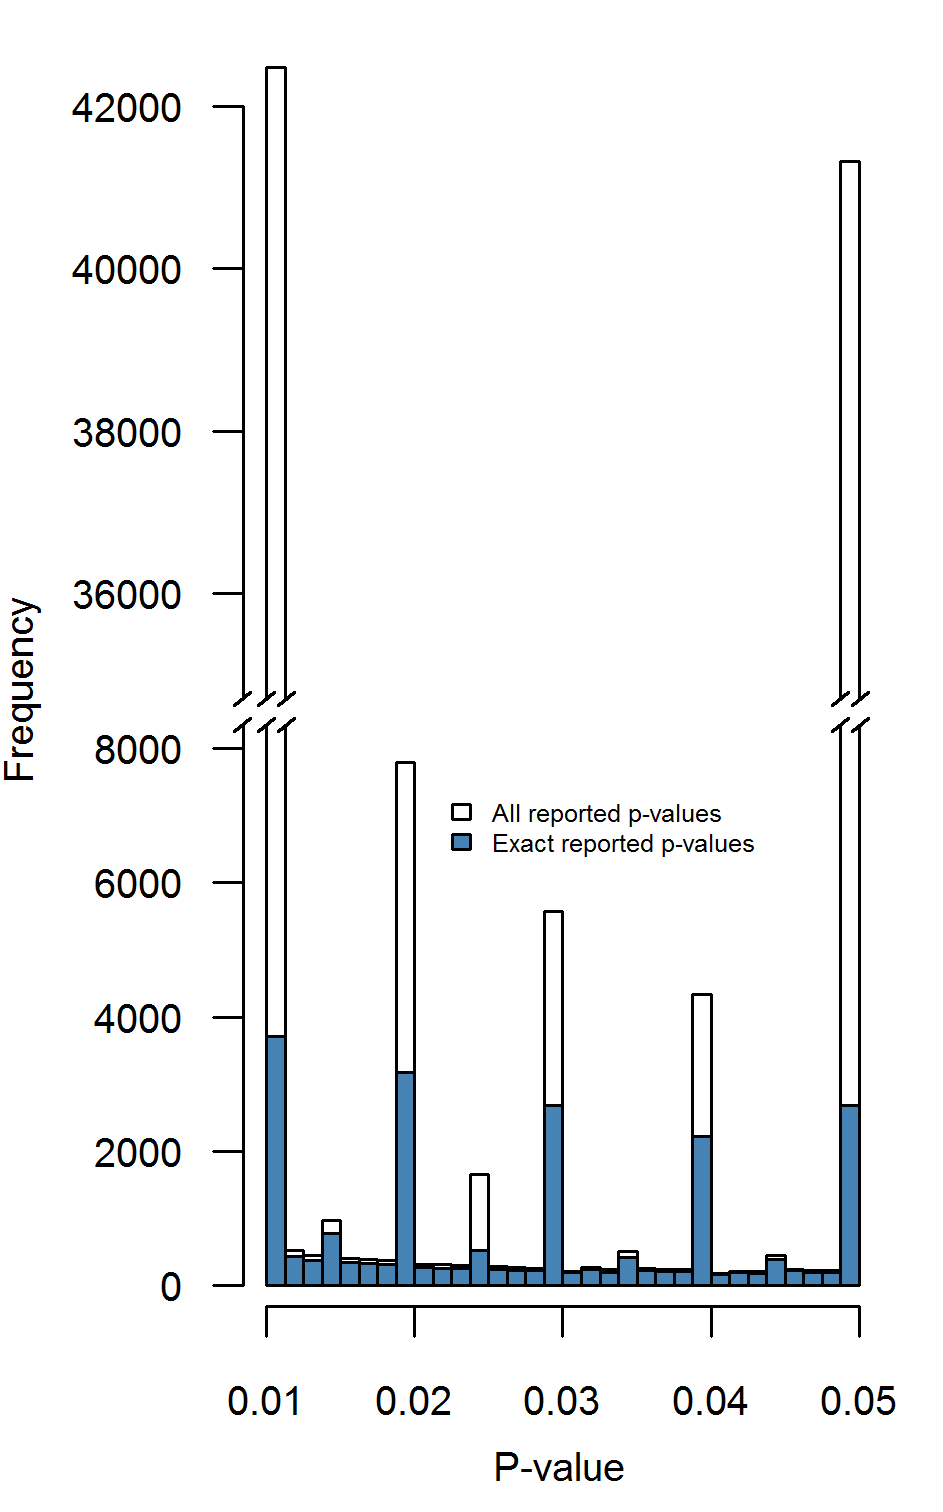
\includegraphics[width=13.1in]{assets/figures/bump-fig2} 

}

\caption{Distributions of all reported $p$-values (white) and exactly reported $p$-values (blue) across eight psychology journals. Binwidth = .00125.}\label{fig:bump-fig2}
\end{figure}

To investigate whether this observed bump below .05 across exactly
reported \(p\)-values originates from one or multiple journals, we
performed the Caliper test on the exactly reported \(p\)-values per
journal. Table \ref{tab:report} shows the results for these tests. The
results indicate that there is sufficient and reliable evidence for a
bump below .05 (i.e., \(Pr>.5\)) for the journals DP and JPSP and
sufficient evidence, but debatable reliability for JAP, where the
results depend on the binwidth. However, the other five journals show no
evidence for a bump below .05 in exactly reported \(p\)-values at all.
In other words, the bump below .05 in exactly reported \(p\)-values is
mainly driven by the journals DP, JAP, and JPSP.

The Caliper test results for reported \(p\)-values indicate two things:
(i) including inexactly reported \(p\)-values has a large impact on the
\(p\)-value distribution and (ii) a bump below .05 is also found when
only considering exactly reported \(p\)-values. Because inexact
reporting of \(p\)-values causes excess at certain points of the
\(p\)-value (e.g., the significance threshold .05; Ridley et al.
\protect\hyperlink{ref-doi:10.1111ux2fj.1420-9101.2006.01291.x}{2007}),
we recommend only inspecting exactly reported \(p\)-values when
examining \(p\)-value distributions.

\begin{landscape}\begin{table}[t]

\caption{\label{tab:report}Caliper test for exactly reported p-values per journal for different binwidths.}
\centering
\resizebox{\linewidth}{!}{
\begin{tabular}{lllllllllllllllll}
\toprule
\multicolumn{1}{c}{Binwidth} & \multicolumn{4}{c}{0.00125} & \multicolumn{4}{c}{0.0025} & \multicolumn{4}{c}{0.005} & \multicolumn{4}{c}{0.01} \\
\cmidrule(l{3pt}r{3pt}){1-1} \cmidrule(l{3pt}r{3pt}){2-5} \cmidrule(l{3pt}r{3pt}){6-9} \cmidrule(l{3pt}r{3pt}){10-13} \cmidrule(l{3pt}r{3pt}){14-17}
 & $x$ & $N$ & $Pr$ & $p$ & $x$ & $N$ & $Pr$ & $p$ & $x$ & $N$ & $Pr$ & $p$ & $x$ & $N$ & $Pr$ & $p$\\
\midrule
\rowcolor{gray!6}  All & \textbf{2,682} & \textbf{4,900} & \textbf{0.547} & \textbf{<.001} & \textbf{2,881} & \textbf{5,309} & \textbf{0.543} & \textbf{<.001} & \textbf{3,308} & \textbf{6,178} & \textbf{0.535} & \textbf{<.001} & \textbf{4,218} & \textbf{8,129} & \textbf{0.519} & \textbf{<.001}\\
DP & \textbf{319} & \textbf{531} & \textbf{0.601} & \textbf{<.001} & \textbf{336} & \textbf{567} & \textbf{0.593} & \textbf{<.001} & \textbf{383} & \textbf{653} & \textbf{0.587} & \textbf{<.001} & \textbf{464} & \textbf{843} & \textbf{0.55} & \textbf{0.002}\\
\rowcolor{gray!6}  FP & 96 & 193 & 0.497 & 0.557 & 105 & 227 & 0.463 & 0.884 & 141 & 304 & 0.464 & 0.906 & 215 & 458 & 0.469 & 0.912\\
JAP & \textbf{78} & \textbf{131} & \textbf{0.595} & \textbf{0.018} & \textbf{82} & \textbf{137} & \textbf{0.599} & \textbf{0.013} & 85 & 154 & 0.552 & 0.113 & 101 & 183 & 0.552 & 0.092\\
\rowcolor{gray!6}  JCCP & 246 & 517 & 0.476 & 0.874 & 267 & 562 & 0.475 & 0.889 & 308 & 641 & 0.48 & 0.848 & 395 & 823 & 0.48 & 0.882\\
\addlinespace
JEPG & 147 & 285 & 0.516 & 0.318 & 159 & 310 & 0.513 & 0.346 & 195 & 375 & 0.52 & 0.235 & 258 & 509 & 0.507 & 0.395\\
\rowcolor{gray!6}  JPSP & \textbf{1,252} & \textbf{2,097} & \textbf{0.597} & \textbf{<.001} & \textbf{1310} & \textbf{2,207} & \textbf{0.594} & \textbf{<.001} & \textbf{1,408} & \textbf{2,399} & \textbf{0.587} & \textbf{<.001} & \textbf{1,623} & \textbf{2,869} & \textbf{0.566} & \textbf{<.001}\\
PLOS & 307 & 649 & 0.473 & 0.921 & 366 & 760 & 0.482 & 0.854 & 489 & 1000 & 0.489 & 0.766 & 744 & 1558 & 0.478 & 0.964\\
\rowcolor{gray!6}  PS & 237 & 497 & 0.477 & 0.859 & 256 & 539 & 0.475 & 0.886 & 299 & 652 & 0.459 & 0.984 & 418 & 886 & 0.472 & 0.957\\
\bottomrule
\end{tabular}}
\end{table}
\end{landscape}

Considering only exactly reported \(p\)-values, there is sufficient
evidence for a bump below .05 in the journals DP, JAP, and JPSP, but not
in the remaining five journals (i.e., FP, JCCP, JEPG, PLOS, PS). A
tentative explanation of the bump of \(p\)-values just below .05 for DP,
JAP, and JPSP may be that QRPs that aim to obtain barely significant
results are more frequent in the fields of these journals. However,
another explanation may be that scientists in these fields are more
prone to exactly report \(p\)-values just below .05 (e.g., to emphasize
they are really smaller than .05) than \(p\)-values considerably smaller
than .05.

\subsection{\texorpdfstring{Recalculated \(p\)-value
distributions}{Recalculated p-value distributions}}\label{recalculated-p-value-distributions}

\subsubsection{\texorpdfstring{Recalculated when reported
\(p=.05\)}{Recalculated when reported p=.05}}\label{recalculated-when-reported-p.05}

Results for reported \(p\)-values remain inconclusive with regard to the
distribution of \(p\)-values, due to potential rounding or errors
(Bakker and Wicherts
\protect\hyperlink{ref-doi:10.3758ux2fs13428-011-0089-5}{2011}; Nuijten,
Hartgerink, et al.
\protect\hyperlink{ref-doi:10.3758ux2fs13428-015-0664-2}{2015}; Veldkamp
et al.
\protect\hyperlink{ref-doi:10.1371ux2fjournal.pone.0114876}{2014}).
Rounding and errors could result in an over-representation of
\(p\)-values \(\leq.05\). To investigate the plausibility of this
notion, we inspected recalculated \(p\)-values when \(p=.05\) was
reported (i.e., 2,470 values). Figure \ref{fig:bump-fig3} indicates that
\(p\)-values that were reported as .05 show remarkable spread when
recalculated, which indicates that the reported \(p\)-value might
frequently be rounded or incorrect, assuming that the reported test
statistics are correct. More specifically, 67.45\% of \(p\)-values
reported as .05 were larger than .05 when recalculated and 32.55\% were
smaller than .05. This percentage does not greatly vary across journals
(range 58.8\%-73.4\% compared to 67.45\%). Taking into account rounding
possibilities (i.e., widening the range of correct \(p\)-values to
.045-.055), these percentages become 13.81\% and 7.85\%, respectively,
meaning incorrect reporting of at least 21.66\% of the \(p\)-values that
were reported as .05. In comparison, \(p\)-values reported as
\(p=.04, p=.03,\) or \(p=.02\) show smaller proportions of downward
rounding when compared to \(p=.05\) (i.e., 53.33\%, 54.32\%, 50.38\%,
respectively compared to 67.45\%). When taking into account potential
rounding errors in the initial reporting of \(p\)-values, the
discrepancy remains but becomes smaller (i.e., 11.74\%, 9.57\%, 8.03\%,
respectively compared to 13.81\%). These results provide direct evidence
for the QRP \enquote{incorrect rounding of \(p\)-value} (John,
Loewenstein, and Prelec
\protect\hyperlink{ref-doi:10.1177ux2f0956797611430953}{2012}), which
contributes to a bump or monotonic excess just below .05.

\begin{figure}[h]

{\centering 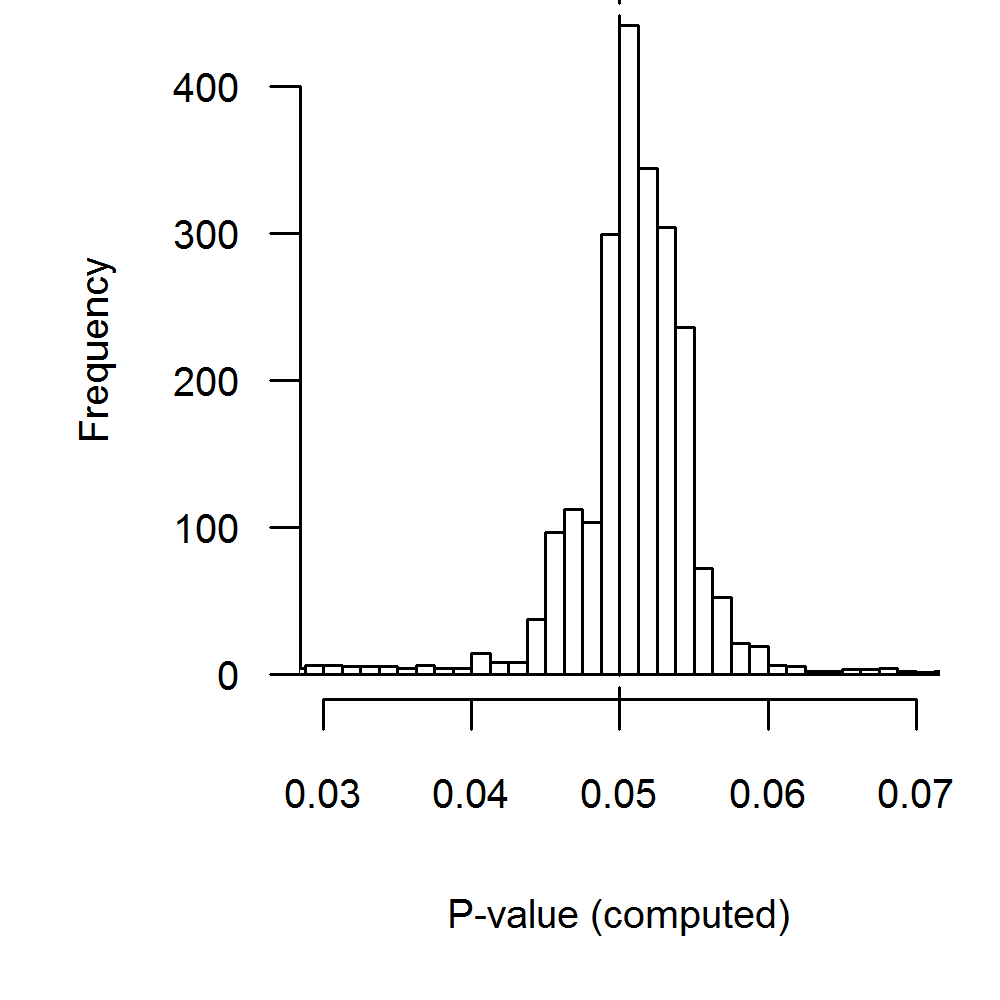
\includegraphics[width=13.89in]{assets/figures/bump-fig3} 

}

\caption{Distribution of recalculated $p$-values where the $p$-value is reported as $p=.05$. 9.7 percent of the results fall outside the range of the plot, with 3.6 percent at the left tail and 6.1 percent at the right tail. Binwidth = .00125}\label{fig:bump-fig3}
\end{figure}

The discrepancy between recalculated \(p\)-values and \(p\)-values
reported as equal to .05 highlights the importance of using recalculated
\(p\)-values when underlying effect distributions are estimated as in
\(p\)-uniform and \(p\)-curve (Van Assen, Van Aert, and Wicherts
\protect\hyperlink{ref-doi:10.1037ux2fmet0000025}{2015}; Simonsohn,
Nelson, and Simmons
\protect\hyperlink{ref-doi:10.1037ux2fa0033242}{2014}). When interested
in inspecting the \(p\)-value distribution, reported \(p\)-values can
substantially distort the \(p\)-value distribution, such that results
become biased if we rely solely on the reported \(p\)-value. Such a
discrepancy indicates potential rounding of \(p\)-values, erroneous
reporting of \(p\)-values, or strategic reporting of \(p\)-values. The
\(p\)-value distortions can be (partially) corrected for by
recalculating \(p\)-values based on reported test statistics.
Additionally, potential distortions to the distribution at the third
decimal place due to the rounding of \(p\)-values to the second decimal
(Hartgerink
\protect\hyperlink{ref-doi:10.7717ux2fpeerj.3068}{2017}\protect\hyperlink{ref-doi:10.7717ux2fpeerj.3068}{b})
is also solved by recalculating \(p\)-values. We continue with
recalculated \(p\)-values in our following analyses.

\subsubsection{\texorpdfstring{Recalculated
\(p\)-values}{Recalculated p-values}}\label{recalculated-p-values}

Figure \ref{fig:bump-fig4} shows the distribution of all recalculated
\(p\)-values (i.e., set of 256,393 results) and of recalculated
\(p\)-values whenever the reported \(p\)-value is exact (i.e., set of
68,776 results). The recalculated \(p\)-value distribution is markedly
smoother than the reported \(p\)-value distribution (see Figure
\ref{fig:bump-fig2}) due to the absence of rounded \(p\)-values.

\begin{figure}[h]

{\centering 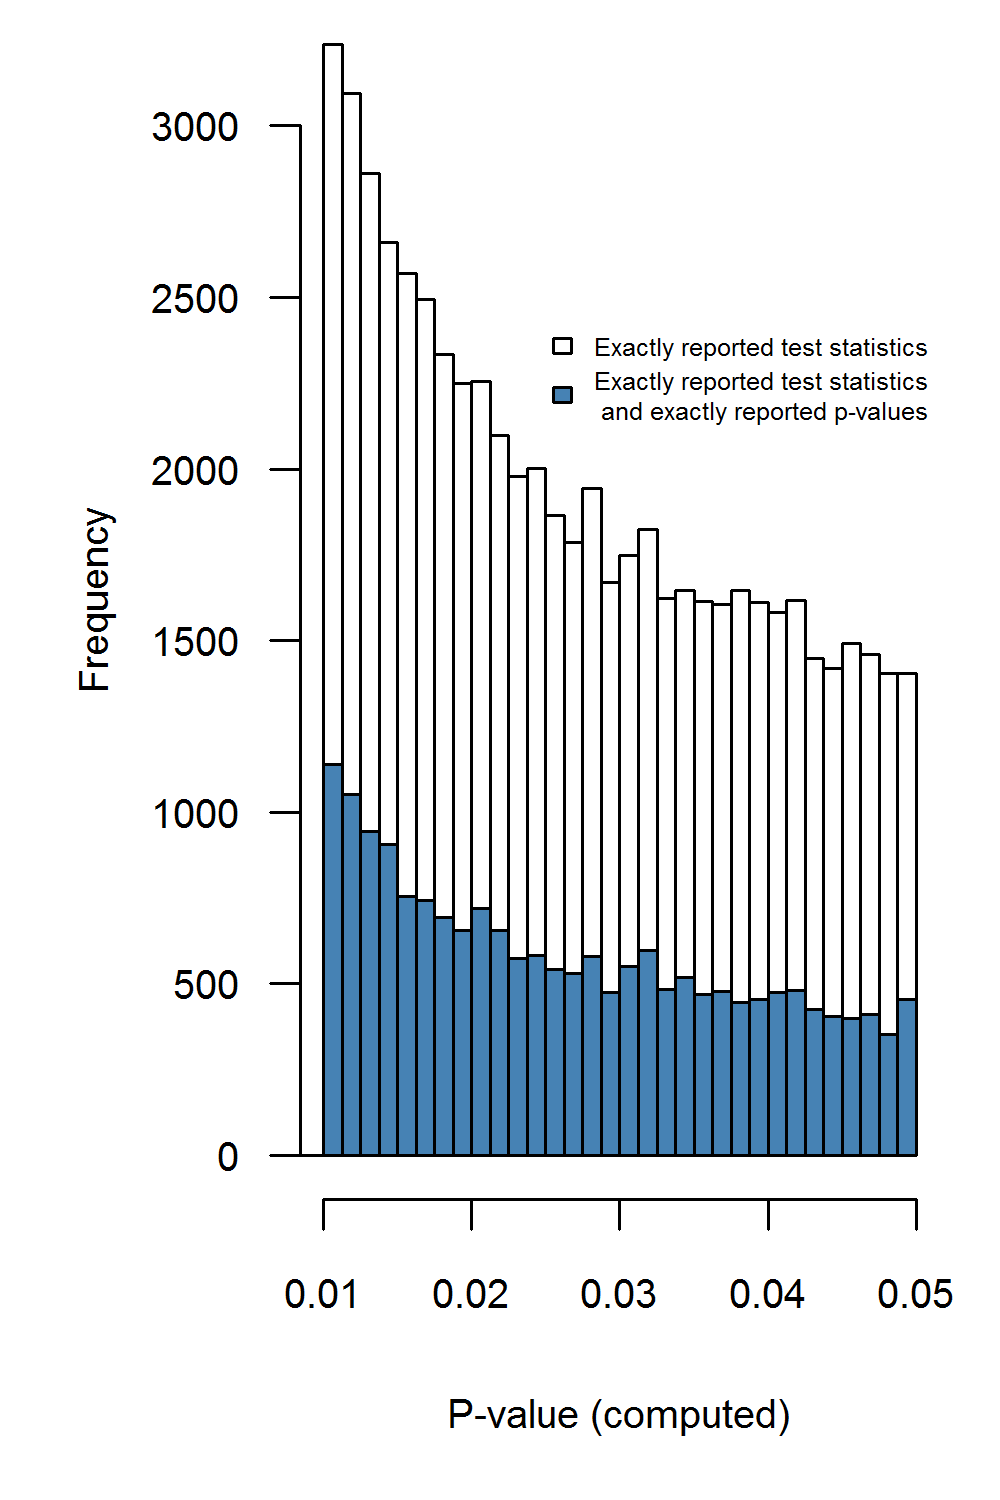
\includegraphics[width=0.6\linewidth]{assets/figures/bump-fig4} 

}

\caption{Recalculated $p$-values for exactly reported test statistics (white bars), and recalculated $p$-values for exactly reported test statistics where $p$-values are also exactly reported (blue bars). Binwidth = .00125}\label{fig:bump-fig4}
\end{figure}

After inspecting all recalculated \(p\)-values, we did not observe a
bump just below .05, \(N=2,808,Pr=.5,p=0.508\). When we analyzed the
recalculated \(p\)-values per journal (Table \ref{tab:recalculated1}),
there is no evidence for a bump below .05 in any of the journals.
Additionally, we inspected all recalculated \(p\)-values that resulted
from exactly reported \(p\)-values. For this subset we did observe a
bump below .05, \(N=809,Pr=0.564,p=0.000165\) (blue histogram in Figure
\ref{fig:bump-fig4}) for the smallest binwidth (i.e., .00125), but this
effect was not robust across larger binwidths, as shown in Table
\ref{tab:recalculated2}. This table also specifies the results for a
bump below .05 per journal, with sufficient evidence of a bump only in
JPSP. This finding, however, was only observed for binwidths .00125 and
.0025, not for larger binwidths. Considering the results from the
recalculated \(p\)-values, there is sparse evidence for the presence of
a bump below .05, opposed to previously claimed widespread evidence
(Masicampo and Lalande
\protect\hyperlink{ref-doi:10.1080ux2f17470218.2012.711335}{2012};
Leggett et al.
\protect\hyperlink{ref-doi:10.1080ux2f17470218.2013.863371}{2013}; Head
et al.
\protect\hyperlink{ref-doi:10.1371ux2fjournal.pbio.1002106}{2015}\protect\hyperlink{ref-doi:10.1371ux2fjournal.pbio.1002106}{b}).
Moreover, interpretation of the bump for JPSP is not straightforward; it
may also be that authors of JPSP are more prone to report exact test
statistics if the \(p\)-value is just below .05 than whenever
\(p\)-values are considerably smaller than .05.

\begin{landscape}\begin{table}[t]

\caption{\label{tab:recalculated1}Caliper test for exactly recalculated p-values per journal for different binwidths.}
\centering
\resizebox{\linewidth}{!}{
\begin{tabular}{lllrrllrrllrrllrl}
\toprule
\multicolumn{1}{c}{Binwidth} & \multicolumn{4}{c}{0.00125} & \multicolumn{4}{c}{0.0025} & \multicolumn{4}{c}{0.005} & \multicolumn{4}{c}{0.01} \\
\cmidrule(l{3pt}r{3pt}){1-1} \cmidrule(l{3pt}r{3pt}){2-5} \cmidrule(l{3pt}r{3pt}){6-9} \cmidrule(l{3pt}r{3pt}){10-13} \cmidrule(l{3pt}r{3pt}){14-17}
 & $x$ & $N$ & $Pr$ & $p$ & $x$ & $N$ & $Pr$ & $p$ & $x$ & $N$ & $Pr$ & $p$ & $x$ & $N$ & $Pr$ & $p$\\
\midrule
\rowcolor{gray!6}  All & 1,404 & 2,808 & 0.500 & 0.508 & 2,808 & 5,761 & 0.487 & 0.973 & 5,761 & 11,824 & 0.487 & 0.997 & 11,824 & 25,142 & 0.470 & >.999\\
DP & 184 & 382 & 0.482 & 0.779 & 382 & 829 & 0.461 & 0.989 & 829 & 1,710 & 0.485 & 0.900 & 1,710 & 3,579 & 0.478 & 0.996\\
\rowcolor{gray!6}  FP & 30 & 69 & 0.435 & 0.886 & 69 & 172 & 0.401 & 0.996 & 172 & 376 & 0.457 & 0.956 & 376 & 799 & 0.471 & 0.955\\
JAP & 73 & 145 & 0.503 & 0.500 & 145 & 270 & 0.537 & 0.124 & 270 & 556 & 0.486 & 0.765 & 556 & 1,168 & 0.476 & 0.952\\
\rowcolor{gray!6}  JCCP & 160 & 308 & 0.519 & 0.265 & 308 & 633 & 0.487 & 0.763 & 633 & 1,267 & 0.500 & 0.522 & 1,267 & 2,706 & 0.468 & >.999\\
\addlinespace
JEPG & 81 & 164 & 0.494 & 0.593 & 164 & 332 & 0.494 & 0.608 & 332 & 683 & 0.486 & 0.778 & 683 & 1,535 & 0.445 & >.999\\
\rowcolor{gray!6}  JPSP & 640 & 1,268 & 0.505 & 0.379 & 1,268 & 2,557 & 0.496 & 0.668 & 2,557 & 5,174 & 0.494 & 0.802 & 5,174 & 10,976 & 0.471 & >.999\\
PLOS & 125 & 260 & 0.481 & 0.752 & 260 & 541 & 0.481 & 0.828 & 541 & 1,170 & 0.462 & 0.995 & 1,170 & 2,544 & 0.460 & >.999\\
\rowcolor{gray!6}  PS & 111 & 212 & 0.524 & 0.268 & 212 & 427 & 0.496 & 0.577 & 427 & 888 & 0.481 & 0.880 & 888 & 1,835 & 0.484 & 0.919\\
\bottomrule
\end{tabular}}
\end{table}
\end{landscape}

\begin{landscape}\begin{table}[t]

\caption{\label{tab:recalculated2}Caliper tests for exactly recalculated and exactly reported p-values per journal, including alternative binwidths.}
\centering
\resizebox{\linewidth}{!}{
\begin{tabular}{lllllllllllrrllrl}
\toprule
\multicolumn{1}{c}{Binwidth} & \multicolumn{4}{c}{0.00125} & \multicolumn{4}{c}{0.0025} & \multicolumn{4}{c}{0.005} & \multicolumn{4}{c}{0.01} \\
\cmidrule(l{3pt}r{3pt}){1-1} \cmidrule(l{3pt}r{3pt}){2-5} \cmidrule(l{3pt}r{3pt}){6-9} \cmidrule(l{3pt}r{3pt}){10-13} \cmidrule(l{3pt}r{3pt}){14-17}
 & $x$ & $N$ & $Pr$ & $p$ & $x$ & $N$ & $Pr$ & $p$ & $x$ & $N$ & $Pr$ & $p$ & $x$ & $N$ & $Pr$ & $p$\\
\midrule
\rowcolor{gray!6}  All & \textbf{456} & \textbf{809} & \textbf{0.564} & \textbf{<.001} & 809 & 1,617 & 0.5 & 0.5 & 1,617 & 3,403 & 0.475 & 0.998 & 3,403 & 7,402 & 0.460 & 1\\
DP & 46 & 87 & 0.529 & 0.334 & 87 & 185 & 0.47 & 0.811 & 185 & 358 & 0.517 & 0.281 & 358 & 756 & 0.474 & 0.932\\
\rowcolor{gray!6}  FP & 15 & 27 & 0.556 & 0.351 & 27 & 87 & 0.31 & >.999 & 87 & 192 & 0.453 & 0.915 & 192 & 437 & 0.439 & 0.995\\
JAP & 8 & 20 & 0.4 & 0.868 & \textbf{20} & \textbf{29} & \textbf{0.69} & \textbf{0.031} & 29 & 65 & 0.446 & 0.839 & 65 & 141 & 0.461 & 0.844\\
\rowcolor{gray!6}  JCCP & 43 & 78 & 0.551 & 0.214 & 78 & 161 & 0.484 & 0.682 & 161 & 364 & 0.442 & 0.988 & 364 & 780 & 0.467 & 0.971\\
\addlinespace
JEPG & 27 & 50 & 0.54 & 0.336 & 50 & 98 & 0.51 & 0.46 & 98 & 209 & 0.469 & 0.834 & 209 & 479 & 0.436 & 0.998\\
\rowcolor{gray!6}  JPSP & \textbf{184} & \textbf{305} & \textbf{0.603} & \textbf{<.001} & \textbf{305} & \textbf{547} & \textbf{0.558} & \textbf{0.004} & 547 & 1,117 & 0.490 & 0.764 & 1,117 & 2,451 & 0.456 & >.999\\
PLOS & 76 & 149 & 0.51 & 0.435 & 149 & 323 & 0.461 & 0.926 & 323 & 698 & 0.463 & 0.978 & 698 & 1,470 & 0.475 & 0.975\\
\rowcolor{gray!6}  PS & 57 & 93 & 0.613 & 0.019 & 93 & 187 & 0.497 & 0.558 & 187 & 400 & 0.468 & 0.912 & 400 & 888 & 0.450 & 0.999\\
\bottomrule
\end{tabular}}
\end{table}
\end{landscape}

\subsection{Excessive significance over
time}\label{excessive-significance-over-time}

The regression results of the development of a bump below .05 over time,
based on recalculated \(p\)-values, are shown in Table \ref{tab:excess}.
Results indicate that there is no evidence for a linear relation between
publication year and the degree to which a bump of \(p\)-values below
.05 is present across the different binwidths (only results for binwidth
.00125 are presented; results for the other binwidths available at
\href{https://osf.io/96kbc/}{osf.io/96kbc/}). Conversely, for PLOS there
is some evidence for a minor increase of a bump throughout the years
(\(b=.072,p=.039\)), but this result is not robust for binwidths .0025,
.005, and .01. These results contrast with Leggett et al.
(\protect\hyperlink{ref-doi:10.1080ux2f17470218.2013.863371}{2013}), who
found a linear relation between time and the degree to which a bump
occurred for JEPG and JPSP. Hence, based on the period 1985-2013, our
findings contrast with the increase of a bump below .05 for the period
1965-2005 in psychology (Leggett et al.
\protect\hyperlink{ref-doi:10.1080ux2f17470218.2013.863371}{2013}). In
other words, our results of the Caliper test indicate that, generally
speaking, there is no evidence for an increasing prevalence of
\(p\)-values just below .05 or of QRPs causing such a bump in
psychology.

\begin{table}[!h]

\caption{\label{tab:excess}Linear regression coefficients as a test of increasing excess of $p$-values just below .05.}
\centering
\resizebox{\linewidth}{!}{
\begin{tabular}{lllllll}
\toprule
 & Timespan & Coefficient & Estimate & $SE$ & $t$ & $p$\\
\midrule
\rowcolor{gray!6}  All & 1985-2013 & Intercept & 0.007 & 0.017 & 0.392 & 0.698\\
All &  & Years (centered) & -0.001 & 0.001 & -0.492 & 0.627\\
\rowcolor{gray!6}  DP & 1985-2013 & Intercept & -0.043 & 0.056 & -0.769 & 0.448\\
DP &  & Years (centered) & 0.001 & 0.003 & 0.193 & 0.849\\
\rowcolor{gray!6}  FP & 2010-2013 & Intercept & -0.182 & 0.148 & -1.233 & 0.343\\
\addlinespace
FP &  & Years (centered) & 0.055 & 0.079 & 0.694 & 0.56\\
\rowcolor{gray!6}  JAP & 1985-2013 & Intercept & 0.041 & 0.081 & 0.504 & 0.619\\
JAP &  & Years (centered) & -0.001 & 0.005 & -0.208 & 0.837\\
\rowcolor{gray!6}  JCCP & 1985-2013 & Intercept & 0.077 & 0.058 & 1.315 & 0.2\\
JCCP &  & Years (centered) & -0.006 & 0.004 & -1.546 & 0.134\\
\addlinespace
\rowcolor{gray!6}  JEPG & 1985-2013 & Intercept & -0.022 & 0.124 & -0.176 & 0.862\\
JEPG &  & Years (centered) & 0.001 & 0.007 & 0.097 & 0.924\\
\rowcolor{gray!6}  JPSP & 1985-2013 & Intercept & -0.002 & 0.027 & -0.062 & 0.951\\
JPSP &  & Years (centered) & 0 & 0.002 & -0.005 & 0.996\\
\rowcolor{gray!6}  PLOS & 2006-2013 & Intercept & \textbf{-0.382} & \textbf{0.114} & \textbf{-3.344} & \textbf{0.016}\\
\addlinespace
PLOS &  & Years (centered) & \textbf{0.072} & \textbf{0.027} & \textbf{2.632} & \textbf{0.039}\\
\rowcolor{gray!6}  PS & 2003-2013 & Intercept & 0.081 & 0.078 & 1.045 & 0.323\\
PS &  & Years (centered) & -0.009 & 0.013 & -0.669 & 0.52\\
\bottomrule
\multicolumn{7}{l}{\textit{Note: }}\\
\multicolumn{7}{l}{Intercept indicates the degree of excess for the first year of the estimated timespan ($>0$ is excess).}\\
\end{tabular}}
\end{table}

\subsection{\texorpdfstring{Results of two measures based on modeling
\(p\)-value
distributions}{Results of two measures based on modeling p-value distributions}}\label{results-of-two-measures-based-on-modeling-p-value-distributions}

\subsubsection{Simulation study}\label{simulation-study}

Table \ref{tab:simres} shows the results of the two measures for data
simulated with and without data peeking. The column headers show the
mean effect size (i.e., \(\delta\)) and heterogeneity (i.e., \(\tau\))
of the simulated conditions, with the corresponding \(\rho_F\) and
\(\tau_{\rho_F}\) on the Fisher transformed correlation scale. The first
set of rows shows the results for the data simulated without data
peeking, of which we discuss the results first.

\begin{landscape}\begin{table}[t]

\caption{\label{tab:simres}Results of parameter estimation of the distribution of effect sizes and measures of data peeking as a function of population effect size ($\delta$, $\rho_F$), population heterogeneity ($\tau$), and data peeking, for the simulated data. Results are based on all $p$-values 0-1, $p$-values $\leq.05$, and $\leq.00125$.}
\centering
\resizebox{\linewidth}{!}{
\begin{tabular}{lllrrrrrrrrlllrrrrrrrrlllrrrrrrrrlllrrrrrrrrlllrrrrrrrrlllrrrrrrrrlllrrrrrrrrlllrrrrrrrrlllrrrrrrrrlllrrrrrrrrlllrrrrrrrr}
\toprule
\multicolumn{3}{c}{ } & \multicolumn{4}{c}{$\tau=0$} & \multicolumn{4}{c}{$\tau=.15$} \\
\cmidrule(l{3pt}r{3pt}){4-7} \cmidrule(l{3pt}r{3pt}){8-11}
 & $p$-values &  & $\delta=0,\rho_{F}=0$ & $\delta=.2,\rho_{F}=.099$ & $\delta=.5,\rho_{F}=.247$ & $\delta=.8,\rho_{F}=.390$ & $\delta=0,\rho_{F}=0$ & $\delta=.2,\rho_{F}=.099$ & $\delta=.5,\rho_{F}=.247$ & $\delta=.8,\rho_{F}=.390$\\
\midrule
\rowcolor{gray!6}  Without data peeking & 0-1 & $\hat{\rho}_{F}$ & 0 & 0.103 & 0.258 & 0.413 & 0 & 0.103 & 0.258 & 0.413\\
 &  & $\hat{\tau}_{\rho_F}$ & 0 & 0 & 0 & 0 & 0.077 & 0.077 & 0.077 & 0.077\\
\rowcolor{gray!6}   & 0-.05 & $\hat{\rho}_{F}$ & 0 & 0.103 & 0.258 & 0.413 & 0 & 0.103 & 0.258 & 0.413\\
 &  & $\hat{\tau}_{\rho_F}$ & 0 & 0 & 0 & 0.001 & 0.077 & 0.077 & 0.077 & 0.077\\
\rowcolor{gray!6}   &  & Misfit $\chi^2$ & 0 & 0 & 0 & 0 & 0 & 0 & 0 & \vphantom{1} 0\\
\addlinespace
 & 0-.00125 & $\hat{\rho}_{F}$ & 0 & 0.103 & 0.258 & 0.413 & 0.1 & 0.107 & 0.259 & 0.413\\
\rowcolor{gray!6}   &  & $\hat{\tau}_{\rho_F}$ & 0 & 0 & 0 & 0.001 & 0.025 & 0.076 & 0.077 & 0.077\\
 &  & Misfit $\chi^2$ & 0 & 0 & 0 & 0 & 0 & 0 & 0 & 0\\
\rowcolor{gray!6}   &  & $D$ & 1 & 1 & 1 & 1 & 1.205 & 1.006 & 1.003 & 1.001\\
With data peeking & 0-.05 & $\hat{\rho}_{F}$ & 0 & 0 & 0.117 & 0.345 & 0 & 0 & 0.075 & 0.36\\
\addlinespace
\rowcolor{gray!6}   &  & $\hat{\tau}_{\rho_F}$ & 0 & 0 & 0 & 0.038 & 0 & 0.055 & 0.137 & 0.091\\
 &  & Misfit $\chi^2$ & 126,267.4 & 50,298.4 & 696.6 & 101.6 & 14,867.6 & 1,209.5 & 576.3 & 340.6\\
\rowcolor{gray!6}   &  & $N$ & 759,812 & 811,296 & 936,517 & 994,974 & 434,660 & 525,023 & 707,650 & 889,681\\
 & 0-.00125 & $\hat{\rho}_{F}$ & 0 & 0.075 & 0.218 & 0.366 & 0.066 & 0.161 & 0.283 & 0.402\\
\rowcolor{gray!6}   &  & $\hat{\tau}_{\rho_F}$ & 0 & 0 & 0 & 0 & 0.036 & 0 & 0 & 0.012\\
\addlinespace
 &  & Misfit $\chi^2$ & 6.9 & 3.2 & 7.1 & 11.8 & 2 & 1.9 & 2.6 & 2.1\\
\rowcolor{gray!6}   &  & $N$ & 9,729 & 21,576 & 95,615 & 350,482 & 14,791 & 34,530 & 124,991 & 366,875\\
 &  & $D$ & 1.977 & 1.976 & 1.835 & 1.166 & 1.628 & 1.62 & 1.472 & 1.164\\
\bottomrule
\end{tabular}}
\end{table}
\end{landscape}

The results for the data without data peeking inform us on (i) whether
the effect size distribution parameters can accurately be recovered
using only very small (\(\leq.00125\)) or small \(p\)-values
(\(\leq.05\)), and (ii) if both measures accurately signal no data
peeking. Note that \(\rho_F\) is slightly overestimated due to
categorizing the \(p\)-value distribution into 40 categories: the
estimates based on all \(p\)-values (i.e., \(\hat{\rho}_F\), first row)
are slightly larger than the population parameter (i.e., \(\rho_F\),
column headers).

Answering the first question of accurate parameter estimates, whenever
there is no heterogeneity (i.e., \(\tau_{\rho_F}=0\)) both \(\rho_F\)
and \(\tau_{\rho_F}\) are accurately recovered. When heterogeneity is
non-zero, the parameters were also accurately recovered, but not when
\(\rho_F=0\). Here, \(\rho_F\) was overestimated (equal to .1) and
\(\tau_{\rho_F}\) underestimated (.025 rather than the true .077), while
at the same time the misfit was negligible.

The latter result, that the effect is overestimated under heterogeneity
when \(\rho_F=0\), is explained by the fact that a \(p\)-value
distribution can accurately be modeled with an infinite range of
negatively correlated values of \(\rho_F\) and \(\tau_{\rho_F}\). An
increase in \(\rho_F\) yields a more right-skewed distribution, which is
hardly distinguishable from the right-skewed distribution caused by an
increase in \(\tau_{\rho_F}\). Hence almost identical \(p\)-value
distributions can be generated with (\(\delta\),\(\tau\)) and some
values (\(\delta^*\),\(\tau^*\)), with \(\delta^*>\mu\) and at the same
time \(\tau^*<\tau\), or \(\delta^*<\mu\) and at the same time
\(\tau^*>\tau\). The similar effects of both parameters on the fitted
\(p\)-value distribution already hint at potential problems for both
measures, because performance of these measures is dependent on accurate
estimates of these parameters.

With respect to the second question, whether the measures accurately
signal the absence of data peeking, the first measure does so in both
homo- and heterogeneous conditions, whereas the second measure correctly
signals absence only under homogeneity. The first measure signals data
peeking if the estimate of \(\rho_F\) is smaller when based on
\(p\leq.05\) than on \(p\leq.00125\). Previously, we already noted that
effect size estimates were identical to population effect sizes under
homogeneity, and equal or \emph{larger} when based on \(p\leq.00125\)
under heterogeneity. This suggests that the first measure behaves well
if there is no data peeking (but see the conclusion section). The second
measure, \(D\), performed well (i.e., was equal to 1) under homogeneity,
but incorrectly suggested data peeking under heterogeneity. For
instance, \(D=1.205\) for \(\rho_F\) = 0 and \(\tau=.15\), which
suggests that 20.5\% more \(p\)-values were observed in the interval
.00125-.05 than were expected based on the \(\hat{\rho}_F\) estimate
even though no data peeking occurred. The explanation for the breakdown
of the performance of \(D\) is that the parameters of the effect size
distribution were not accurately recovered, overestimating the average
effect size and underestimating heterogeneity based on small
\(p\)-values. This yields a lower expected frequency of higher
\(p\)-values (between .00125 and .05), thereby falsely suggesting data
peeking.

The last rows present the results obtained when data peeking does occur.
First, consider the estimates of \(\rho_F\) and the performance of the
first measure of data peeking. The estimates of \(\rho_F\) confirm that
data peeking results in underestimation, particularly if the average
true effect size is not large (i.e., \(\delta=.2\) or \(.5\)). Moreover,
downward bias of \(\rho_F\) decreases when it is estimated on
\(p\)-values \(\leq.00125\) than on \(\leq.05\), accurately signaling
data peeking with the first measure. For instance, if \(\rho_F=.099\)
and \(\tau=0\), \(\hat{\rho}_F=.075\) when based on \(p\)-values
\(\leq.00125\) and \(\hat{\rho}_F=0\) when based on \(p\)-values
\(\leq.05\). Together with the good performance of this measure under no
data peeking, these results suggest that the first measure may be useful
to detect data peeking in practice.

Consider the estimates of \(\tau_{\rho_F}\) and the performance of
\(D\). Similar to conditions under no data peeking, heterogeneity is
grossly underestimated when using \(p\)-values \(\leq.00125\). Hence
\(D\) cannot be expected to perform well under data peeking. Although
\(D\)-values seem to correctly signal data peeking in all conditions and
decrease as expected when the effect size increases, these values do not
correspond to the actual values of data peeking. For instance, consider
the condition with \(\delta=.5\) and \(\tau_{\rho_F}=.15\); of the
582,659 simulated \(p\)-values in interval .00125-.05, 106,241
\(p\)-values were obtained through data-peeking, which yields a true
\(D=1.223\), which is very different from the estimated \(D=1.472\) in
Table \ref{tab:simres}.

Finally, consider the (mis)fit of the estimated \(p\)-value
distribution. Despite the considerable downward bias in heterogeneity
estimate \(\hat{\tau}_{\rho_F}\), the simulated \(p\)-value distribution
is mostly well approximated by the expected \(p\)-value distribution, as
indicated by the small values of the \(\chi^2\) statistic for
\(p\)-values in 0-.00125. Hence, good fit again does not imply accurate
parameter estimates. The misfit of the estimated distribution for
\(p\)-values \(\leq.05\) is indicated by large \(\chi^2\)-values,
particularly when the \(p\)-value distribution is not monotonically
decreasing (which is the case for, e.g., \(\delta=0\)).

To conclude, this simulation study showed that under true homogeneity
both measures of data peeking can accurately signal both absence and
presence of data peeking. However, under true heterogeneity,
heterogeneity is underestimated and the performance of \(D\) breaks
down, while results suggest that comparing estimates of average effect
size, the first measure, may still accurately signal both the absence
and presence of data peeking.

\subsubsection{Applied to data of eight psychology
journals}\label{applied-to-data-of-eight-psychology-journals}

Figure \ref{fig:bump-fig5} depicts the observed \(p\)-value distribution
and the expected \(p\)-value distribution corresponding to the fitted
effect size distribution based on \(p\)-values \(\leq.00125\). Estimates
for \(p\)-values \(\leq.05\) were effect size \(\hat{\rho}_F=0\) and
heterogeneity \(\hat{\tau}_{\rho_F}=.183\), and \(\hat{\rho}_F=.149\)
and \(\hat{\tau}_{\rho_F}=.106\) for \(p\)-values \(\leq.00125\). Note
that we only considered nonnegative values of \(\delta\) in the
estimation procedure. Misfit between observed and expected \(p\)-value
distribution for \(p\leq.00125\) was minor (\(\chi^2=4.1\)), indicating
that the observed \(p\)-values \(\leq.00125\) were well approximated by
the estimated effect size distribution.

\begin{figure}[h]

{\centering 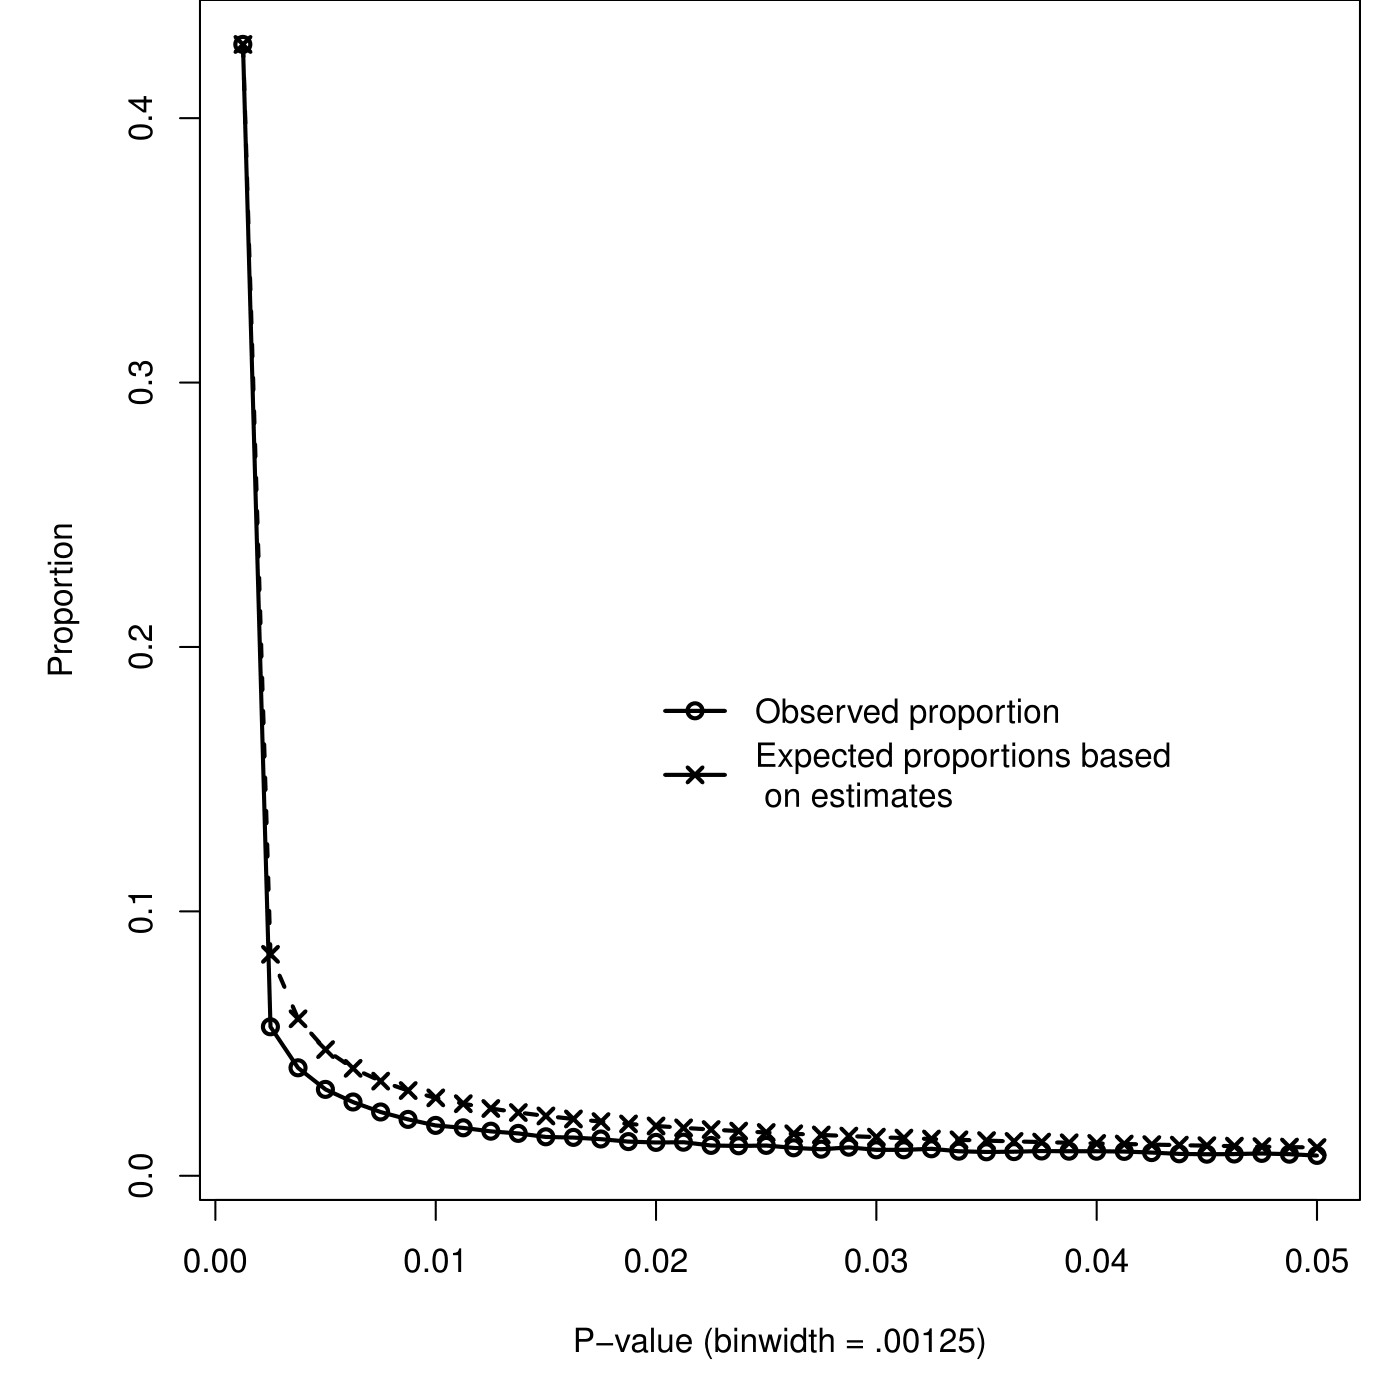
\includegraphics[width=0.8\linewidth]{assets/figures/bump-fig5} 

}

\caption{Observed proportions of $p$-values (circles) and expected proportions of $p$-values based on estimated $\hat{\rho}_F$ and estimated $\hat{\tau}_{\rho_F}$ estimated from 0-.00125 (crosses).}\label{fig:bump-fig5}
\end{figure}

Our first measure suggests practices leading to a monotonic excess of
\(p\)-values below .05, because the estimated effect size based on all
significant \(p\)-values (i.e., 0) is much smaller than the supposedly
more accurate estimate based on only the very small \(p\)-values (i.e.,
.183). Moreover, assuming that effect sizes are normally distributed
with \(\rho_F=0\) and \(\tau_{\rho_F}=.183\), combined with the degrees
of freedom of the observed effects, implies that only 27.5\% of all
effects would be statistically significant. However, of all reported
\(p\)-values, 74.7\% were statistically significant, but this difference
may at least partly be caused by other factors such as publication bias.
It is highly unlikely that the average true effect size underlying
statistically significant results in psychology is truly zero. It
remains undecided, however, whether this very low estimate is mainly due
to QRPs leading to a downward bias of the effect size estimate, or to a
misspecification of the model, an issue we revisit later in the paper.

For the second measure that compares the ratio of observed and expected
\(p\)-values below .05, we found \(D=.701\), which does not suggest data
peeking but \emph{under}-reporting of \(p\)-values (29.9\%) in the
\(p\)-value interval .00125-.05. The simulation results, however, have
already demonstrated that the measure \(D\) performs badly under effect
size heterogeneity. Since heterogeneity is underlying the observed data,
we conclude that the measure \(D\) is not useful for investigating
evidence of a bump or monotonic excess of \(p\)-values.

\section{Limitations and conclusions}\label{limitations-and-conclusions}

Before concluding, some limitations of our method to collect
\(p\)-values need to be addressed. First, \texttt{statcheck} (Epskamp
and Nuijten \protect\hyperlink{ref-statcheck}{2016}; Nuijten,
Hartgerink, et al.
\protect\hyperlink{ref-doi:10.3758ux2fs13428-015-0664-2}{2015}), the R
package used to collect the observed data, extracts all APA test results
reported in the text of an article, but not those reported in tables.
Hence, our selection of results is potentially not representative of all
reported results and systematically excludes results that are not
reported to APA standards. Second, our analysis assumed that test
statistics other than \(p\)-values were accurately reported. If test
statistics and degrees of freedom are incorrectly reported, recalculated
\(p\)-values are wrong as well. We identified some erroneous test
statistics (e.g., \(df_1=0\) and \(r>1\)), but do not know how often
errors in reported test statistics and df occur and how these errors may
have affected our results. We assumed that \(p\)-value errors were made
due to the overemphasis on them in current day research.

In light of conflicting findings and interpretations, we aimed to
provide final answers to the questions (1) Does a bump or monotonic
excess of \(p\)-values below .05 exist in psychology? and (2) Did
evidence for a bump increase over time in psychology? Answering these
research questions may inform us on the prevalence of QRPs and its
development over time in psychology. Using \texttt{statcheck}, we
extracted and analyzed 258,050 test results conforming to APA-style
across 30,710 articles from eight high impact journals in psychology,
and distinguished between results with inexactly reported \(p\)-values,
exactly reported \(p\)-values, and recalculated \(p\)-values. The basic
idea underlying our analyses is that QRPs distort the \(p\)-value
distribution. We argued that only some QRPs yield an excess of
\(p\)-values just below .05, and show that QRPs sometimes yield a bump
and sometimes only monotonic excess of \(p\)-values just below .05. We
used the Caliper test to test for a bump, and suggested two measures to
examine monotonic excess.

Starting with the existence of a bump in psychology, we drew the
following conclusions. First, \emph{inexactly} reported \(p\)-values are
not useful for analyses of \(p\)-value distributions. Second, a bump in
\emph{exactly} reported \(p\)-values indeed exists in psychology
journals DP, JAP, and JPSP. QRPs leading to just significant
\(p\)-values can explain these bumps, but we also cannot rule out the
explanation that scientists in these particular journals are more prone
to exactly report \(p\)-values just below .05 (e.g., to emphasize they
are really smaller than .05) than \(p\)-values considerably smaller than
.05. Third, contradicting Leggett et al.
(\protect\hyperlink{ref-doi:10.1080ux2f17470218.2013.863371}{2013}), the
bump and evidence of a bump in psychology did not increase over the
years. Fourth, when analyzing only the \emph{exactly} reported
\(p\)-values equal to .05, clear and direct evidence was obtained for
the QRP \enquote{incorrect rounding of \(p\)-value} (John, Loewenstein,
and Prelec
\protect\hyperlink{ref-doi:10.1177ux2f0956797611430953}{2012}). Evidence
of this QRP, which contributed to the bump in exactly reported
\(p\)-values in psychology, was found in all psychology journals. Fifth,
after removing reporting errors and analyzing the \emph{recalculated}
reported \(p\)-values, evidence of a bump was found only for JPSP.
Again, this may have been caused by QRPs or by scientists being more
prone to report all test statistics when \(p\)-values are just below .05
than if they are considerable smaller than zero.

The conclusions obtained with the two measures investigating the bump
and monotonic excess are not satisfactory. First, performance of both
measures is dependent on accurately recovering parameters of the effect
size distribution, which turned out to be difficult; estimates of effect
size heterogeneity and average effect size are highly correlated and
unstable when based on only statistically significant findings. Second,
simulations show that one of the measures, \(D\), does not accurately
assess the QRP data peeking when effect sizes are heterogeneous. Third,
even though performance of the second measure (i.e., difference between
effect sizes based on contaminated and supposedly uncontaminated
\(p\)-values) is affected by estimation problems, it correctly signaled
data peeking in the simulations. Fourth, when applying the second
measure to the observed distribution of significant \(p\)-values in
psychology, the measure found evidence of monotonic excess of
\(p\)-values; the average effect size estimate based on all these
\(p\)-values was 0, which seems very unrealistic, and suggests the use
of QRPs in psychology leading to \(p\)-values just below .05.

Notwithstanding the outcome of the second measure, suggesting QRPs that
cause monotonic excess, we do not consider it as direct evidence of such
QRPs in psychology. Lakens (p.3; 2015) suggests that \enquote{it is
essential to use a model of \(p\)-value distributions before drawing
conclusions about the underlying reasons for specific distributions of
\(p\)-values extracted from the scientific literature.} We explicitly
modeled the effect size distribution and by using the degrees of freedom
of test results also model the effect sizes' power and the \(p\)-value
distribution. But we fear this is not and cannot be sufficient. First of
all, we could not accurately recover the effect size distribution under
heterogeneity in our simulation study, even if all assumptions of our
model were met. This rendered measure \(D\) unfruitful when there is
heterogeneity, and severely limits the usefulness of the second measure
that compares estimated average effect sizes. Second, devising other
models may yield other results and thereby other interpretations
(Benjamini and Hechtlinger
\protect\hyperlink{ref-doi:10.1093ux2fbiostatisticsux2fkxt032}{2013};
Goodman
\protect\hyperlink{ref-doi:10.1093ux2fbiostatisticsux2fkxt035}{2013};
Lakens
\protect\hyperlink{ref-doi:10.7717ux2fpeerj.1142}{2015}\protect\hyperlink{ref-doi:10.7717ux2fpeerj.1142}{b};
De Winter and Dodou
\protect\hyperlink{ref-doi:10.7717ux2fpeerj.733}{2015}).

Results of all the aforementioned models are most likely not robust to
violations of their assumptions. For instance, we assume a normal
distribution of true effect sizes. This assumption is surely violated,
since the reported \(p\)-values arise from a mixture of many different
types of effects, such as very large effects (manipulation checks),
effects corresponding to main hypotheses, and zero effects
(\enquote{control} variables). Additionally, consider the QRPs
themselves; we examined the effect of only one QRP, data peeking, in one
of its limited variants. Other QRPs exist that also increase the
prevalence of \(p\)-values just below .05, such as multiple
operationalizations of a measure and selecting the first one to be
significant. Other QRPs even increase the frequency of very small
\(p\)-values (Van Aert, Wicherts, and Van Assen
\protect\hyperlink{ref-doi:10.1177ux2f1745691616650874}{2016}). We deem
it impossible to accurately model QRPs and their effects, considering
the difficulties we already demonstrated for modeling the \(p\)-value
distribution generated using a single QRP that was clearly defined. To
conclude, we fear that Gelman and O'Rourke
(\protect\hyperlink{ref-doi:10.1093ux2fbiostatisticsux2fkxt034}{2013})
may be right when suggesting that drawing conclusions with regard to any
QRP based on modeling \(p\)-value distributions obtained from
automatically extracted results is unfruitful.

On the other hand, we do recommend modeling effect size and \(p\)-value
distributions of results that all intend to test the same hypothesis, to
prevent contamination by irrelevant test results (Bishop and Thompson
\protect\hyperlink{ref-doi:10.7717ux2fpeerj.1715}{2016}; Simonsohn,
Simmons, and Nelson
\protect\hyperlink{ref-doi:10.1037ux2fxge0000104}{2015}). Examples of
methods that focus on similar results are \(p\)-uniform (Van Assen, Van
Aert, and Wicherts
\protect\hyperlink{ref-doi:10.1037ux2fmet0000025}{2015}) and \(p\)-curve
(Simonsohn, Nelson, and Simmons
\protect\hyperlink{ref-doi:10.1037ux2fa0033242}{2014}), which model
statistically significant statistics pertaining to one specific effect
and estimate the effect size based on these statistics while correcting
for publication bias. Further research should reveal if both methods can
also be used to detect and correct for \(p\)-hacking in the context of
estimating one particular effect size. Preliminary results suggest,
however, that detection and correcting for \(p\)-hacking based on
statistics alone is rather challenging (Van Aert, Wicherts, and Van
Assen \protect\hyperlink{ref-doi:10.1177ux2f1745691616650874}{2016}).

\chapter{Too good to be false: Nonsignificant results
revisited}\label{too-good-to-be-false-nonsignificant-results-revisited}

Popper (\protect\hyperlink{ref-isbn:9780415278430}{2002}) falsifiability
serves as one of the main demarcating criteria in the social sciences,
which stipulates that a hypothesis is required to have the possibility
of being proven false to be considered scientific. Within the
theoretical framework of scientific hypothesis testing, accepting or
rejecting a hypothesis is unequivocal, because the hypothesis is either
true or false. Statistical hypothesis testing, on the other hand, is a
probabilistic operationalization of scientific hypothesis testing (Meehl
\protect\hyperlink{ref-doi:10.1016ux2fj.appsy.2004.02.001}{2004}) and,
in lieu of its probabilistic nature, is subject to decision errors. Such
decision errors are the topic of this chapter.

Null Hypothesis Significance Testing (NHST) is the most prevalent
paradigm for statistical hypothesis testing in the social sciences
(American Psychological Association
\protect\hyperlink{ref-isbn:9781433805615}{2010}\protect\hyperlink{ref-isbn:9781433805615}{b}).
In NHST the hypothesis \(H_0\) is tested, where \(H_0\) most often
regards the absence of an effect. If deemed false, an alternative,
mutually exclusive hypothesis \(H_1\) is accepted. These decisions are
based on the \(p\)-value; the probability of the sample data, or more
extreme data, given \(H_0\) is true. If the \(p\)-value is smaller than
the decision criterion \(\alpha\) (typically .05; Nuijten, Hartgerink,
et al. \protect\hyperlink{ref-doi:10.3758ux2fs13428-015-0664-2}{2015}),
\(H_0\) is rejected and \(H_1\) is accepted.

Table \ref{tab:tgtbf-tab1} summarizes the four possible situations that
can occur in NHST. The columns indicate which hypothesis is true in the
population and the rows indicate what is decided based on the sample
data. When there is discordance between the true- and decided
hypothesis, a decision error is made. More specifically, when \(H_0\) is
true in the population, but \(H_1\) is accepted (\('H_1'\)), a Type I
error is made (\(\alpha\)); a false positive (lower left cell). When
\(H_1\) is true in the population and \(H_0\) is accepted (\('H_0'\)), a
Type II error is made (\(\beta\)); a false negative (upper right cell).
However, when the null hypothesis is true in the population and \(H_0\)
is accepted (\('H_0'\)), this is a true negative (upper left cell;
\(1-\alpha\)). The true negative rate is also called specificity of the
test. Conversely, when the alternative hypothesis is true in the
population and \(H_1\) is accepted (\('H_1'\)), this is a true positive
(lower right cell). The probability of finding a statistically
significant result if \(H_1\) is true is the power (\(1-\beta\)), which
is also called the sensitivity of the test. Power is a positive function
of the (true) population effect size, the sample size, and the alpha of
the study, such that higher power can always be achieved by altering
either the sample size or the alpha level (Aberson
\protect\hyperlink{ref-Aberson2010-xa}{2010}).

\begin{table}[!h]

\caption{\label{tab:tgtbf-tab1}Summary table of possible NHST results. Columns indicate the true situation in the population, rows indicate the decision based on a statistical test. The true positive probability is also called power and sensitivity, whereas the true negative rate is also called specificity.}
\centering
\resizebox{\linewidth}{!}{
\begin{tabular}{llll}
\toprule
\multicolumn{2}{c}{ } & \multicolumn{2}{c}{Population} \\
\cmidrule(l{3pt}r{3pt}){3-4}
 &  & $H_0$ & $H_1$\\
\midrule
\rowcolor{gray!6}  Decision & $’H_0’$ & $1-\alpha$, true negative & $\beta$, false negative [Type II error]\\
 & $’H_1’$ & $\alpha$, false positive [Type I error] & $1-\beta$, true positive\\
\bottomrule
\end{tabular}}
\end{table}

Unfortunately, NHST has led to many misconceptions and
misinterpretations (Goodman
\protect\hyperlink{ref-doi:10.1053ux2fj.seminhematol.2008.04.003}{2008};
Bakan \protect\hyperlink{ref-doi:10.1037ux2fh0020412}{1966}). The most
serious mistake relevant to our chapter is that many researchers accept
the null-hypothesis and claim no effect in case of a statistically
nonsignificant effect (about 60\%, see Hoekstra et al.
\protect\hyperlink{ref-doi:10.3758ux2fbf03213921}{2006}). Hence, most
researchers overlook that the outcome of hypothesis testing is
probabilistic (if the null-hypothesis is true, or the alternative
hypothesis is true and power is less than 1) and interpret outcomes of
hypothesis testing as reflecting the absolute truth. At least partly
because of mistakes like this, many researchers ignore the possibility
of false negatives and false positives and they remain pervasive in the
literature.

Recent debate about false positives has received much attention in
science and psychological science in particular. The Reproducibility
Project Psychology (RPP), which replicated 100 effects reported in
prominent psychology journals in 2008, found that only 36\% of these
effects were statistically significant in the replication (Open Science
Collaboration
\protect\hyperlink{ref-doi:10.1126ux2fscience.aac4716}{2015}). Besides
in psychology, reproducibility problems have also been indicated in
economics (Camerer et al.
\protect\hyperlink{ref-doi:10.1126ux2fscience.aaf0918}{2016}) and
medicine (Begley and Ellis
\protect\hyperlink{ref-doi:10.1038ux2f483531a}{2012}). Although these
studies suggest substantial evidence of false positives in these fields,
replications show considerable variability in resulting effect size
estimates (R. A. Klein et al.
\protect\hyperlink{ref-doi:10.1027ux2f1864-9335ux2fa000178}{2014};
Stanley and Spence
\protect\hyperlink{ref-doi:10.1177ux2f1745691614528518}{2014}).
Therefore caution is warranted when wishing to draw conclusions on the
presence of an effect in individual (original or replication) studies
(Open Science Collaboration
\protect\hyperlink{ref-doi:10.1126ux2fscience.aac4716}{2015}; Gilbert et
al. \protect\hyperlink{ref-doi:10.1126ux2fscience.aad7243}{2016};
Anderson et al.
\protect\hyperlink{ref-doi:10.1126ux2fscience.aad9163}{2016}).

The debate about false positives is driven by the current overemphasis
on statistical significance of research results (Giner-Sorolla
\protect\hyperlink{ref-doi:10.1177ux2f1745691612457576}{2012}). This
overemphasis is substantiated by the finding that more than 90\% of
results in the psychological literature are statistically significant
(Open Science Collaboration
\protect\hyperlink{ref-doi:10.1126ux2fscience.aac4716}{2015}; Sterling,
Rosenbaum, and Weinkam
\protect\hyperlink{ref-doi:10.2307ux2f2684823}{1995}; Sterling
\protect\hyperlink{ref-doi:10.2307ux2f2282137}{1959}) despite low
statistical power due to small sample sizes (Cohen
\protect\hyperlink{ref-doi:10.1037ux2fh0045186}{1962}; Sedlmeier and
Gigerenzer
\protect\hyperlink{ref-doi:10.1037ux2f0033-2909.105.2.309}{1989};
Marszalek et al.
\protect\hyperlink{ref-doi:10.2466ux2f03.11.pms.112.2.331-348}{2011};
Bakker, Dijk, and Wicherts
\protect\hyperlink{ref-doi:10.1177ux2f1745691612459060}{2012}).
Consequently, publications have become biased by overrepresenting
statistically significant results (Greenwald
\protect\hyperlink{ref-doi:10.1037ux2fh0076157}{1975}), which generally
results in effect size overestimation in both individual studies
(Nuijten, Hartgerink, et al.
\protect\hyperlink{ref-doi:10.3758ux2fs13428-015-0664-2}{2015}) and
meta-analyses (Van Assen, Van Aert, and Wicherts
\protect\hyperlink{ref-doi:10.1037ux2fmet0000025}{2015}; Lane and Dunlap
\protect\hyperlink{ref-doi:10.1111ux2fj.2044-8317.1978.tb00578.x}{1978};
Rothstein \protect\hyperlink{ref-isbn:9780470870150}{2005}; Borenstein
et al. \protect\hyperlink{ref-isbn:9781119964377}{2011}). The
overemphasis on statistically significant effects has been accompanied
by questionable research practices (QRPs; John, Loewenstein, and Prelec
\protect\hyperlink{ref-doi:10.1177ux2f0956797611430953}{2012}) such as
erroneously rounding p-values towards significance, which for example
occurred for 13.8\% of all \(p\)-values reported as \enquote{\(p =.05\)}
in articles from eight major psychology journals in the period 1985-2013
(Hartgerink et al.
\protect\hyperlink{ref-doi:10.7717ux2fpeerj.1935}{2016}).

The concern for false positives has overshadowed the concern for false
negatives in the recent debate, which seems unwarranted. Cohen
(\protect\hyperlink{ref-doi:10.1037ux2fh0045186}{1962}) was the first to
indicate that psychological science was (severely) underpowered, which
is defined as the chance of finding a statistically significant effect
in the sample being lower than 50\% when there is truly an effect in the
population. This has not changed throughout the subsequent fifty years
(Bakker, Dijk, and Wicherts
\protect\hyperlink{ref-doi:10.1177ux2f1745691612459060}{2012}; Fraley
and Vazire
\protect\hyperlink{ref-doi:10.1371ux2fjournal.pone.0109019}{2014}).
Given that the complement of true positives (i.e., power) are false
negatives, no evidence either exists that the problem of false negatives
has been resolved in psychology. Moreover, Fiedler, Kutzner, and Krueger
(Fiedler, Kutzner, and Krueger
\protect\hyperlink{ref-doi:10.1177ux2f1745691612462587}{2012}) expressed
the concern that an increased focus on false positives is too
shortsighted because false negatives are more difficult to detect than
false positives. They also argued that, because of the focus on
statistically significant results, negative results are less likely to
be the subject of replications than positive results, decreasing the
probability of detecting a false negative. Additionally, the Positive
Predictive Value (PPV, the number of statistically significant effects
that are true; Ioannidis
\protect\hyperlink{ref-doi:10.1371ux2fjournal.pmed.0020124}{2005}) has
been a major point of discussion in recent years, whereas the Negative
Predictive Value (NPV) has rarely been mentioned.

The research objective of the current chapter is to examine evidence for
false negative results in the psychology literature. To this end, we
inspected a large number of nonsignificant results from eight flagship
psychology journals. First, we compared the observed effect
distributions of nonsignificant results for eight journals (combined and
separately) to the expected null distribution based on simulations,
where a discrepancy between observed and expected distribution was
anticipated (i.e., presence of false negatives). Second, we propose to
use the Fisher test to test the hypothesis that \(H_0\) is true for all
nonsignificant results reported in a paper, which we show to have high
power to detect false negatives in a simulation study. Third, we applied
the Fisher test to the nonsignificant results in 14,765 psychology
papers from these eight flagship psychology journals to inspect how many
papers show evidence of at least one false negative result. Fourth, we
examined evidence of false negatives in reported gender effects. Gender
effects are particularly interesting, because gender is typically a
control variable and not the primary focus of studies. Hence we expect
little \(p\)-hacking and substantial evidence of false negatives in
reported gender effects in psychology. Finally, as another application,
we applied the Fisher test to the 64 nonsignificant replication results
of the RPP (Open Science Collaboration
\protect\hyperlink{ref-doi:10.1126ux2fscience.aac4716}{2015}) to examine
whether at least one of these nonsignificant results may actually be a
false negative.

\section{Theoretical framework}\label{theoretical-framework}

We begin by reviewing the probability density function of both an
individual \(p\)-value and a set of independent \(p\)-values as a
function of population effect size. Subsequently, we apply the
Kolmogorov-Smirnov test to inspect whether a collection of
nonsignificant results across papers deviates from what would be
expected under the \(H_0\). We also propose an adapted Fisher method to
test whether nonsignificant results deviate from \(H_0\) within a paper.
These methods will be used to test whether there is evidence for false
negatives in the psychology literature.

\subsection{\texorpdfstring{Distributions of
\emph{p}-values}{Distributions of p-values}}\label{distributions-of-p-values}

The distribution of one \(p\)-value is a function of the population
effect, the observed effect and the precision of the estimate. When the
population effect is zero, the probability distribution of one
\(p\)-value is uniform. When there is a non-zero effect, the probability
distribution is right-skewed. More specifically, as sample size or true
effect size increases, the probability distribution of one \(p\)-value
becomes increasingly right-skewed. These regularities also generalize to
a set of independent \(p\)-values, which are uniformly distributed when
there is no population effect and right-skew distributed when there is a
population effect, with more right-skew as the population effect and/or
precision increases (Fisher
\protect\hyperlink{ref-Fisher1925-jl}{1925}).

Considering that the present chapter focuses on false negatives, we
primarily examine nonsignificant \(p\)-values and their distribution.
Since the test we apply is based on nonselected \(p\)-values, it
requires random variables distributed between 0 and 1. We apply the
following transformation to each nonsignificant \(p\)-value that is
selected

\begin{equation}
p^*_i=\frac{p_i-\alpha}{1-\alpha}
\label{eq:pistar}
\end{equation}

where \(p_i\) is the reported nonsignificant \(p\)-value, \(\alpha\) is
the selected significance cutoff (i.e., \(\alpha=.05\)), and \(p^*_i\)
the transformed \(p\)-value. Note that this transformation retains the
distributional properties of the original \(p\)-values for the selected
nonsignificant results. Both one-tailed and two-tailed tests can be
included in this way.

\subsection{Testing for false negatives: the Fisher
test}\label{testing-for-false-negatives-the-fisher-test}

We applied the Fisher test to inspect whether the distribution of
observed nonsignificant \(p\)-values deviates from those expected under
\(H_0\). The Fisher test was initially introduced as a meta-analytic
technique to synthesize results across studies (Fisher
\protect\hyperlink{ref-Fisher1925-jl}{1925}; Hedges and Olkin
\protect\hyperlink{ref-Hedges1985-dy}{1985}). When applied to
transformed nonsignificant \(p\)-values (see Equation \eqref{eq:pistar})
the Fisher test tests for evidence against \(H_0\) in a set of
nonsignificant \(p\)-values. In other words, the null hypothesis we test
with the Fisher test is that all included nonsignificant results are
true negatives. The Fisher test statistic is calculated as

\begin{equation}
\chi^2_{2k}=-2\sum\limits^k_{i=1}ln(p^*_i)
\label{eq:fishertest}
\end{equation}

where \(k\) is the number of nonsignificant \(p\)-values and \(\chi^2\)
has \(2k\) degrees of freedom. A larger \(\chi^2\) value indicates more
evidence for at least one false negative in the set of \(p\)-values. We
conclude that there is sufficient evidence of at least one false
negative result, if the Fisher test is statistically significant at
\(\alpha=.10\), similar to tests of publication bias that also use
\(\alpha=.10\) (Sterne, Gavaghan, and Egger
\protect\hyperlink{ref-doi:10.1016ux2fs0895-43560000242-0}{2000};
Ioannidis and Trikalinos
\protect\hyperlink{ref-doi:10.1177ux2f1740774507079441}{2007}; Francis
\protect\hyperlink{ref-doi:10.3758ux2fs13423-012-0227-9}{2012}).

We estimated the power of detecting false negatives with the Fisher test
as a function of sample size \(N\), true correlation effect size
\(\eta\), and \(k\) nonsignificant test results (the full procedure is
described in Appendix A). The three levels of sample size used in our
simulation study (33, 62, 119) correspond to the 25th, 50th (median) and
75th percentiles of the degrees of freedom of reported \(t\), \(F\), and
\(r\) statistics in eight flagship psychology journals (see Application
1 below). Degrees of freedom of these statistics are directly related to
sample size, for instance, for a two-group comparison including 100
people, df = 98.

Table \ref{tab:tgtbf-tab2} summarizes the results for the simulations of
the Fisher test when the nonsignificant \(p\)-values are generated by
either small- or medium population effect sizes. Results for all 5,400
conditions can be found on the OSF
(\href{https://osf.io/qpfnw}{osf.io/qpfnw}). The results indicate that
the Fisher test is a powerful method to test for a false negative among
nonsignificant results. For example, for small true effect sizes
(\(\eta=.1\)), 25 nonsignificant results from medium samples result in
85\% power (7 nonsignificant results from large samples yield 83\%
power). For medium true effects (\(\eta=.25\)), three nonsignificant
results from small samples (\(N=33\)) already provide 89\% power for
detecting a false negative with the Fisher test. For large effects
(\(\eta=.4\)), two nonsignificant results from small samples already
almost always detects the existence of false negatives (not shown in
Table \ref{tab:tgtbf-tab2}).

\begin{table}[!h]

\caption{\label{tab:tgtbf-tab2}Power of Fisher test to detect false negatives for small- and medium effect sizes (i.e., $\eta=.1$ and $\eta=.25$), for different sample sizes (i.e., $N$) and number of test results (i.e., $k$). Results of each condition are based on 10,000 iterations. Power was rounded to 1 whenever it was larger than .9995.}
\centering
\begin{tabular}{lrrrrrr}
\toprule
\multicolumn{1}{c}{ } & \multicolumn{3}{c}{$\eta=.1$} & \multicolumn{3}{c}{$\eta=.25$} \\
\cmidrule(l{3pt}r{3pt}){2-4} \cmidrule(l{3pt}r{3pt}){5-7}
 & $N=33$ & $N=62$ & $N=119$ & $N=33$ & $N=62$ & $N=119$\\
\midrule
\rowcolor{gray!6}  $k = 1$ & 0.151 & 0.211 & 0.341 & 0.575 & 0.852 & 0.983\\
$k = 2$ & 0.175 & 0.267 & 0.459 & 0.779 & 0.978 & 1.000\\
\rowcolor{gray!6}  $k = 3$ & 0.201 & 0.317 & 0.572 & 0.894 & 1.000 & 1.000\\
$k = 4$ & 0.208 & 0.352 & 0.659 & 0.948 & 1.000 & 1.000\\
\rowcolor{gray!6}  $k = 5$ & 0.229 & 0.390 & 0.719 & 0.975 & 1.000 & 1.000\\
\addlinespace
$k = 6$ & 0.251 & 0.434 & 0.784 & 0.990 & 1.000 & 1.000\\
\rowcolor{gray!6}  $k = 7$ & 0.259 & 0.471 & 0.834 & 0.995 & 1.000 & 1.000\\
$k = 8$ & 0.280 & 0.514 & 0.871 & 0.998 & 1.000 & 1.000\\
\rowcolor{gray!6}  $k = 9$ & 0.298 & 0.530 & 0.895 & 1.000 & 1.000 & 1.000\\
$k = 10$ & 0.304 & 0.570 & 0.918 & 1.000 & 1.000 & 1.000\\
\addlinespace
\rowcolor{gray!6}  $k = 15$ & 0.362 & 0.691 & 0.980 & 1.000 & 1.000 & 1.000\\
$k = 20$ & 0.429 & 0.780 & 0.996 & 1.000 & 1.000 & 1.000\\
\rowcolor{gray!6}  $k = 25$ & 0.490 & 0.852 & 1.000 & 1.000 & 1.000 & 1.000\\
$k = 30$ & 0.531 & 0.894 & 1.000 & 1.000 & 1.000 & 1.000\\
\rowcolor{gray!6}  $k = 35$ & 0.578 & 0.930 & 1.000 & 1.000 & 1.000 & 1.000\\
\addlinespace
$k = 40$ & 0.621 & 0.953 & 1.000 & 1.000 & 1.000 & 1.000\\
\rowcolor{gray!6}  $k = 45$ & 0.654 & 0.966 & 1.000 & 1.000 & 1.000 & 1.000\\
$k = 50$ & 0.686 & 0.976 & 1.000 & 1.000 & 1.000 & 1.000\\
\bottomrule
\end{tabular}
\end{table}

To put the power of the Fisher test into perspective, we can compare its
power to reject the null based on one statistically nonsignificant
result (\(k=1\)) with the power of a regular \(t\)-test to reject the
null. If \(\eta=.1\), the power of a regular \(t\)-test equals 0.17,
0.255, 0.467 for sample sizes of 33, 62, 119, respectively; if \(\eta\)
= .25, power values equal 0.813, 0.998, 1 for these sample sizes. The
power values of the regular \(t\)-test are higher than that of the
Fisher test, because the Fisher test does not make use of the more
informative statistically significant findings.

\section{Application 1: Evidence of false negatives in articles across
eight major psychology
journals}\label{application-1-evidence-of-false-negatives-in-articles-across-eight-major-psychology-journals}

To show that statistically nonsignificant results do not warrant the
interpretation that there is truly no effect, we analyzed statistically
nonsignificant results from eight major psychology journals. First, we
investigate if and how much the distribution of reported nonsignificant
effect sizes deviates from what the expected effect size distribution is
if there is truly no effect (i.e., \(H_0\)). Second, we investigate how
many research articles report nonsignificant results and how many of
those show evidence for at least one false negative using the Fisher
test (Fisher \protect\hyperlink{ref-Fisher1925-jl}{1925}). Note that
this application only investigates the evidence of false negatives in
articles, not how authors might interpret these findings (i.e., we do
not assume all these nonsignificant results are interpreted as evidence
for the null).

\subsection{Method}\label{method}

APA style \(t\), \(r\), and \(F\) test statistics were extracted from
eight psychology journals with the \texttt{R} package \texttt{statcheck}
(Nuijten, Hartgerink, et al.
\protect\hyperlink{ref-doi:10.3758ux2fs13428-015-0664-2}{2015}; Epskamp
and Nuijten \protect\hyperlink{ref-statcheck}{2016}). APA style is
defined as the format where the type of test statistic is reported,
followed by the degrees of freedom (if applicable), the observed test
value, and the \(p\)-value (e.g., \(t(85)=2.86, p=.005\); American
Psychological Association
\protect\hyperlink{ref-isbn:9781433805615}{2010}\protect\hyperlink{ref-isbn:9781433805615}{b}).
The \texttt{statcheck} package also recalculates \(p\)-values. We reuse
the data from Nuijten et al. (\url{https://osf.io/gdr4q}; Nuijten,
Hartgerink, et al.
\protect\hyperlink{ref-doi:10.3758ux2fs13428-015-0664-2}{2015}). Table
\ref{tab:tgtbf-tab3} depicts the journals, the timeframe, and summaries
of the results extracted. The database also includes \(\chi^2\) results,
which we did not use in our analyses because effect sizes based on these
results are not readily mapped on the correlation scale. Two erroneously
reported test statistics were eliminated, such that these did not
confound results.

The analyses reported in this chapter use the recalculated \(p\)-values
to eliminate potential errors in the reported \(p\)-values (Bakker and
Wicherts \protect\hyperlink{ref-doi:10.3758ux2fs13428-011-0089-5}{2011};
Nuijten, Hartgerink, et al.
\protect\hyperlink{ref-doi:10.3758ux2fs13428-015-0664-2}{2015}).
However, our recalculated \(p\)-values assumed that all other test
statistics (degrees of freedom, test values of \(t\), \(F\), or \(r\))
are correctly reported. These errors may have affected the results of
our analyses. Since most \(p\)-values and corresponding test statistics
were consistent in our dataset (90.7\%), we do not believe these typing
errors substantially affected our results and conclusions based on them.

\begin{landscape}\begin{table}[t]

\caption{\label{tab:tgtbf-tab3}Summary table of articles downloaded per journal, their mean number of results, and proportion of (non)significant results. Statistical significance was determined using $\alpha=.05$, two-tailed test.}
\centering
\resizebox{\linewidth}{!}{
\begin{tabular}{llllll}
\toprule
Journal Acronym & Time frame & Results & Mean results per article & Significant (\%) & Nonsignificant (\%)\\
\midrule
\rowcolor{gray!6}  Developmental Psychology (DP) & 1985–2013 & 30,920 & 13.5 & 24,584 (79.5\%) & 6,336 (20.5\%)\\
Frontiers in Psychology (FP) & 2010–2013 & 9,172 & 14.9 & 6,595 (71.9\%) & 2,577 (28.1\%)\\
\rowcolor{gray!6}  Journal of Applied Psychology (JAP) & 1985–2013 & 11,240 & 9.1 & 8,455 (75.2\%) & 2,785 (24.8\%)\\
Journal of Consulting and Clinical Psychology (JCCP) & 1985–2013 & 20,083 & 9.8 & 15,672 (78.0\%) & 4,411 (22.0\%)\\
\rowcolor{gray!6}  Journal of Experimental Psychology: General (JEPG) & 1985–2013 & 17,283 & 22.4 & 12,706 (73.5\%) & 4,577 (26.5\%)\\
\addlinespace
Journal of Personality and Social Psychology (JPSP) & 1985–2013 & 91,791 & 22.5 & 69,836 (76.1\%) & 21,955 (23.9\%)\\
\rowcolor{gray!6}  Public Library of Science (PLOS) & 2003–2013 & 28,561 & 13.2 & 19,696 (69.0\%) & 8,865 (31.0\%)\\
Psychological Science (PS) & 2003–2013 & 14,032 & 9 & 10,943 (78.0\%) & 3,089 (22.0\%)\\
\rowcolor{gray!6}  \textit{Totals} & \textit{1985–2013} & \textit{223,082} & \textit{14.3} & \textit{168,487 (75.5\%)} & \textit{54,595 (24.5\%)}\\
\bottomrule
\end{tabular}}
\end{table}
\end{landscape}

First, we compared the observed nonsignificant effect size distribution
(computed with observed test results) to the expected nonsignificant
effect size distribution under \(H_0\). The expected effect size
distribution under \(H_0\) was approximated using simulation. We first
randomly drew an observed test result (with replacement) and
subsequently drew a random nonsignificant \(p\)-value between 0.05 and 1
(i.e., under the distribution of the \(H_0\)). Based on the drawn
\(p\)-value and the degrees of freedom of the drawn test result, we
computed the accompanying test statistic and the corresponding effect
size (for details on effect size computation see Appendix A). This
procedure was repeated 163,785 times, which is three times the number of
observed nonsignificant test results (54,595). The collection of
simulated results approximates the expected effect size distribution
under \(H_0\), assuming independence of test results in the same paper.
We inspected this possible dependency with the intra-class correlation
(\(ICC\)), where \(ICC=1\) indicates full dependency and \(ICC=0\)
indicates full independence. For the set of observed results, the ICC
for nonsignificant \(p\)-values was 0.001, indicating independence of
\(p\)-values within a paper (the ICC of the log odds transformed
\(p\)-values was similar, with \(ICC=0.002\) after excluding
\(p\)-values equal to 1 for computational reasons). The resulting,
expected effect size distribution was compared to the observed effect
size distribution (i) across all journals and (ii) per journal. To test
for differences between the expected and observed nonsignificant effect
size distributions we applied the Kolmogorov-Smirnov test. This is a
non-parametric goodness-of-fit test for equality of distributions, which
is based on the maximum absolute deviation between the independent
distributions being compared (denoted \(D\); Massey
\protect\hyperlink{ref-doi:10.2307ux2f2280095}{1951}).

Second, we applied the Fisher test to test how many research papers show
evidence of at least one false negative statistical result. To
recapitulate, the Fisher test tests whether the distribution of observed
nonsignificant \(p\)-values deviates from the uniform distribution
expected under \(H_0\). In order to compute the result of the Fisher
test, we applied equations \eqref{eq:pistar} and \eqref{eq:fishertest} to
the recalculated nonsignificant \(p\)-values in each paper
(\(\alpha=.05\)).

\subsection{Results}\label{results}

\subsubsection{Observed effect size
distribution.}\label{observed-effect-size-distribution.}

Figure \ref{fig:tgtbf-fig1} shows the distribution of observed effect
sizes (in \(|\eta|\)) across all articles and indicates that, of the
223,082 observed effects, 7\% were zero to small (i.e.,
\(0\leq|\eta|<.1\)), 23\% were small to medium (i.e.,
\(.1\leq|\eta|<.25\)), 27\% medium to large (i.e.,
\(.25\leq|\eta|<.4\)), and 42\% large or larger (i.e., \(|\eta|\geq.4\);
Cohen \protect\hyperlink{ref-isbn:9780805802832}{1988}). This suggests
that the majority of effects reported in psychology is medium or smaller
(i.e., 30\%), which is somewhat in line with a previous study on effect
distributions (Gignac and Szodorai
\protect\hyperlink{ref-doi:10.1016ux2fj.paid.2016.06.069}{2016}). Of the
full set of 223,082 test results, 54,595 (24.5\%) were nonsiginificant,
which is the dataset for our main analyses.

\begin{figure}[h]

{\centering 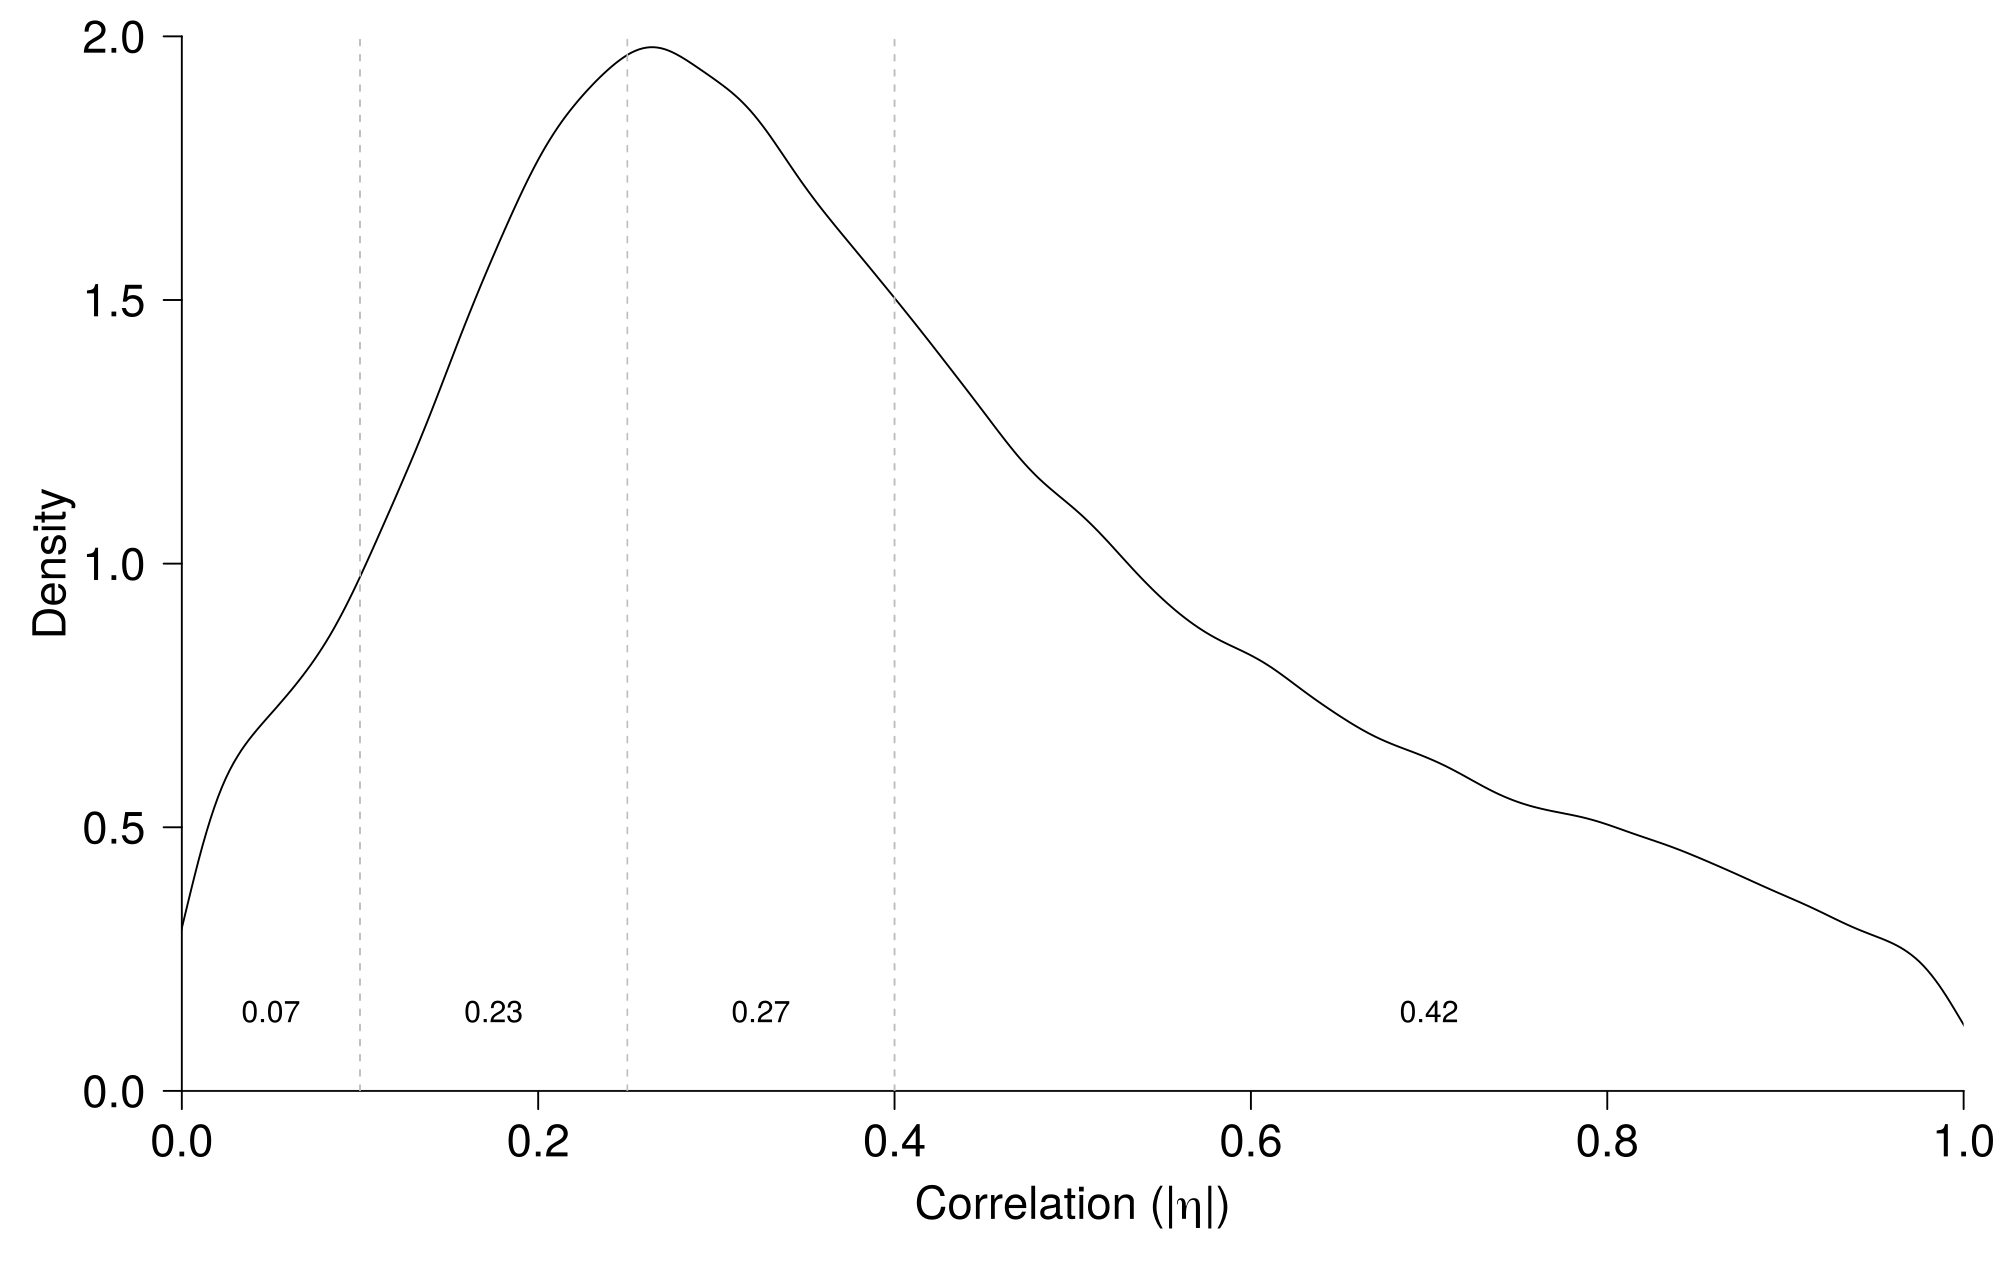
\includegraphics[width=1\linewidth]{assets/figures/tgtbf-fig1.pdf.svg} 

}

\caption{Density of observed effect sizes of results reported in eight psychology journals, with 7 percent of effects in the category none-small, 23 percent small-medium, 27 percent medium-large, and 42 percent beyond large.}\label{fig:tgtbf-fig1}
\end{figure}

Our dataset indicated that more nonsignificant results are reported
throughout the years, strengthening the case for inspecting potential
false negatives. The proportion of reported nonsignificant results
showed an upward trend, as depicted in Figure \ref{fig:tgtbf-fig2}, from
approximately 20\% in the eighties to approximately 30\% of all reported
APA results in 2015.

\begin{figure}[h]

{\centering 
\includegraphics[width=1\linewidth]{assets/figures/tgtbf-fig2.pdf.svg} 

}

\caption{Observed proportion of nonsignificant test results per year.}\label{fig:tgtbf-fig2}
\end{figure}

\subsection{Expected effect size
distribution.}\label{expected-effect-size-distribution.}

For the entire set of nonsignificant results across journals, Figure
\ref{fig:tgtbf-fig3} indicates that there is substantial evidence of
false negatives. Under \(H_0\), 46\% of all observed effects is expected
to be within the range \(0\leq|\eta|<.1\), as can be seen in the left
panel of Figure \ref{fig:tgtbf-fig3} highlighted by the lowest grey line
(dashed). However, of the observed effects, only 26\% fall within this
range, as highlighted by the lowest black line. Similarly, we would
expect 85\% of all effect sizes to be within the range
\(0\leq|\eta|<.25\) (middle grey line), but we observed 14 percentage
points less in this range (i.e., 71\%; middle black line); 96\% is
expected for the range \(0\leq|\eta|<.4\) (top grey line), but we
observed 4 percentage points less (i.e., 92\%; top black line). These
differences indicate that larger nonsignificant effects are reported in
papers than expected under a null effect. This indicates the presence of
false negatives, which is confirmed by the Kolmogorov-Smirnov test,
\(D=0.3\), \(p<.000000000000001\). Results were similar when the
nonsignificant effects were considered separately for the eight
journals, although deviations were smaller for the Journal of Applied
Psychology (see \url{https://osf.io/au3wv/} for results per journal).

\begin{figure}[h]

{\centering 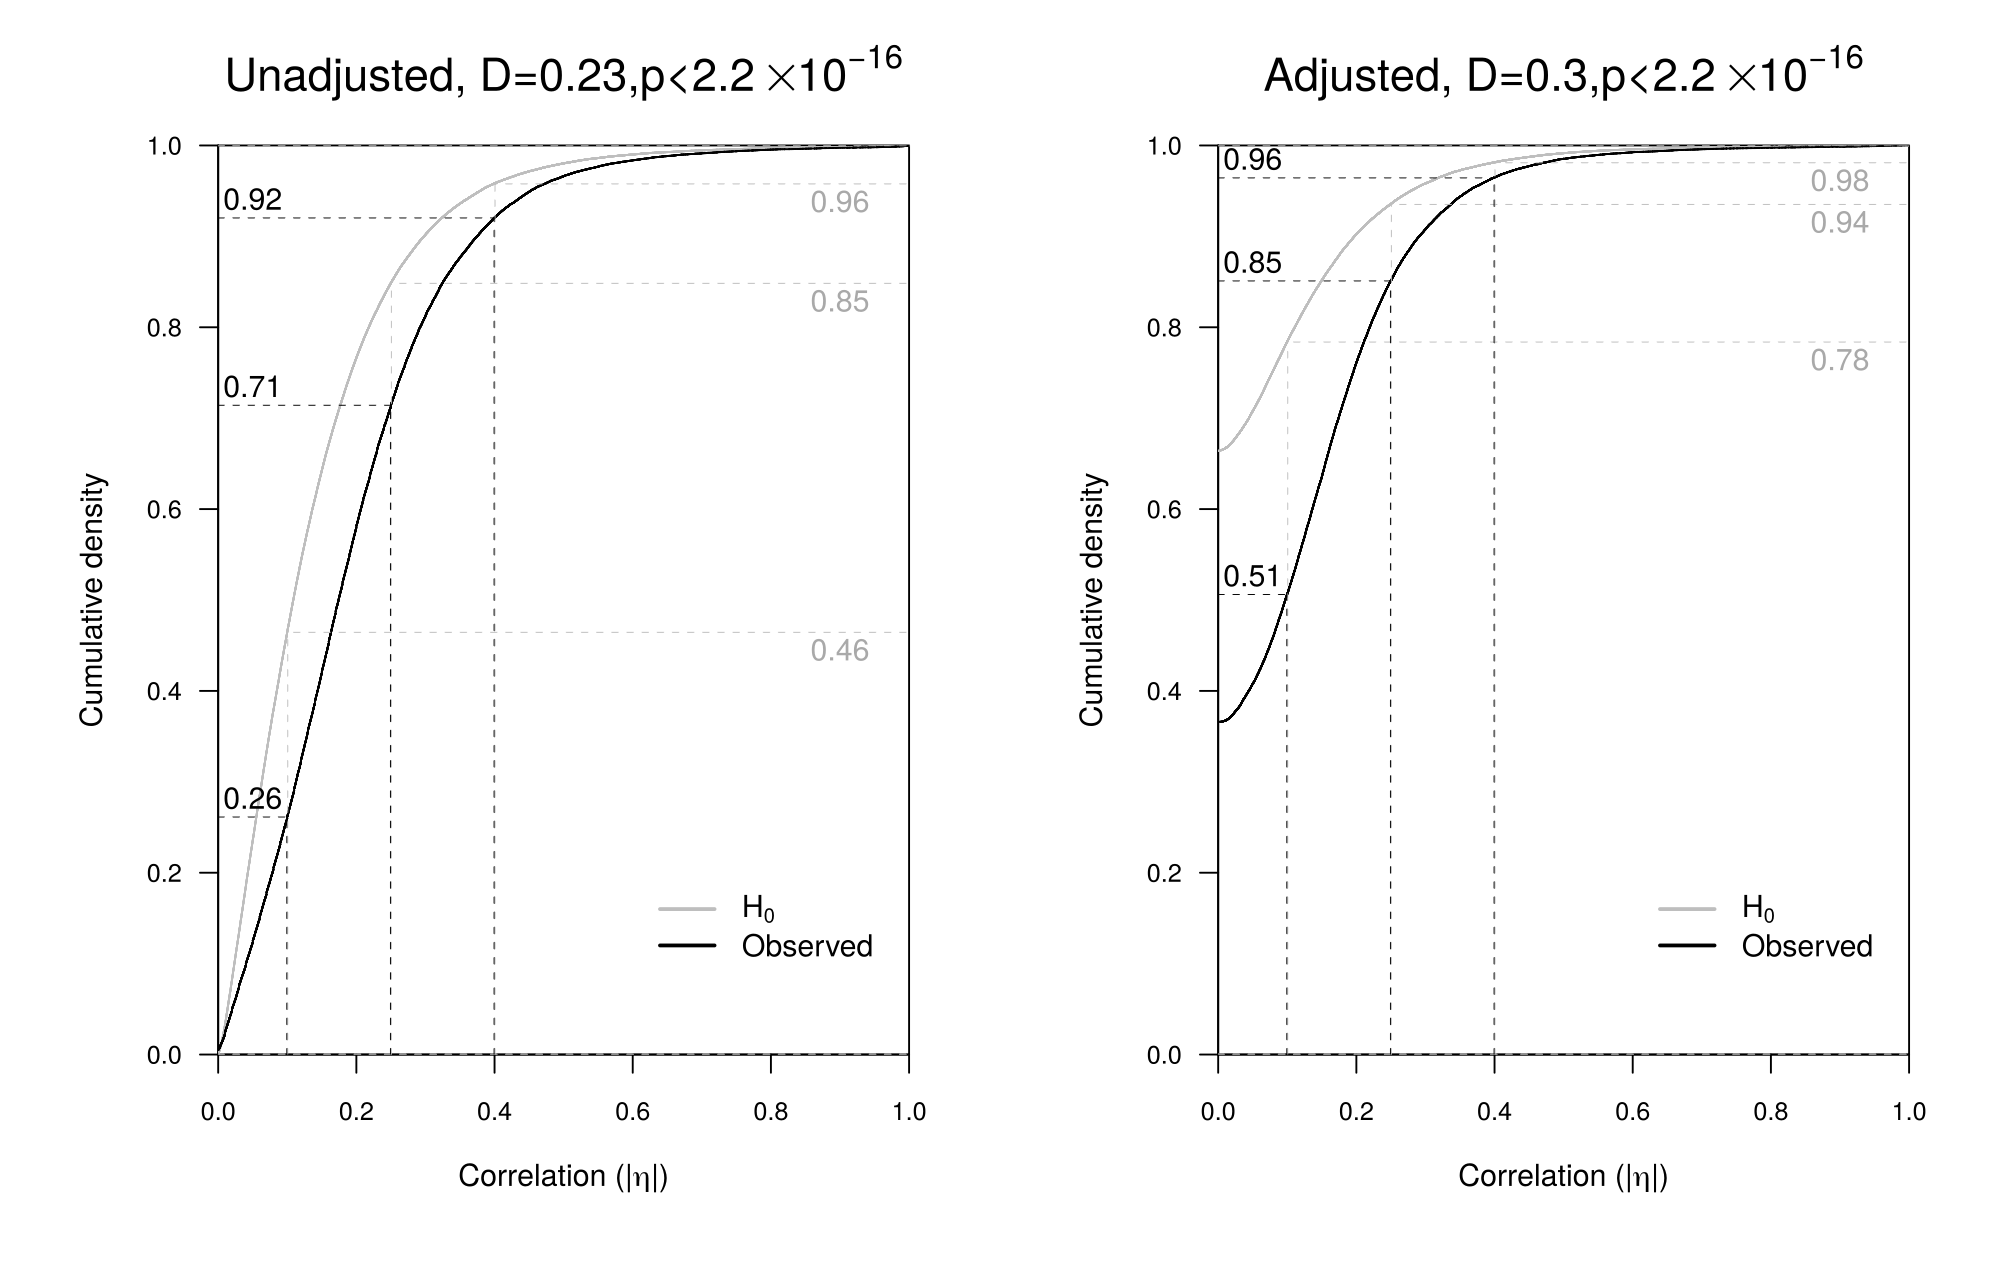
\includegraphics[width=1\linewidth]{assets/figures/tgtbf-fig3.pdf.svg} 

}

\caption{Observed and expected (adjusted and unadjusted) effect size distribution for statistically nonsignificant APA results reported in eight psychology journals. Grey lines depict expected values; black lines depict observed values. The three vertical dotted lines correspond to a small, medium, large effect, respectively. Header includes Kolmogorov-Smirnov test results.}\label{fig:tgtbf-fig3}
\end{figure}

Because effect sizes and their distribution typically overestimate
population effect size \(\eta^2\), particularly when sample size is
small (Voelkle, Ackerman, and Wittmann
\protect\hyperlink{ref-doi:10.1027ux2f1614-2241.3.1.35}{2007}; Hedges
\protect\hyperlink{ref-doi:10.3102ux2f10769986006002107}{1981}), we also
compared the observed and expected adjusted nonsignificant effect sizes
that correct for such overestimation of effect sizes (right panel of
Figure \ref{fig:tgtbf-fig3}; see Appendix A). Such overestimation
affects all effects in a model, both focal and non-focal. The
distribution of adjusted effect sizes of nonsignificant results tells
the same story as the unadjusted effect sizes; observed effect sizes are
larger than expected effect sizes. For instance, the distribution of
adjusted reported effect size suggests 49\% of effect sizes are at least
small, whereas under the \(H_0\) only 22\% is expected.

\subsection{Evidence of false negatives in
articles.}\label{evidence-of-false-negatives-in-articles.}

The Fisher test was applied to the nonsignificant test results of each
of the 14,765 papers separately, to inspect for evidence of false
negatives. More technically, we inspected whether \(p\)-values within a
paper deviate from what can be expected under the \(H_0\) (i.e.,
uniformity). If \(H_0\) is in fact true, our results would be that there
is evidence for false negatives in 10\% of the papers (a meta-false
positive). Table \ref{tab:tgtbf-tab4} shows the number of papers with
evidence for false negatives, specified per journal and per \(k\) number
of nonsignificant test results. The first row indicates the number of
papers that report no nonsignificant results. When \(k=1\), the Fisher
test is simply another way of testing whether the result deviates from a
null effect, conditional on the result being statistically
nonsignificant. Overall results (last row) indicate that 47.1\% of all
articles show evidence of false negatives (i.e.~6,951 articles). Of
articles reporting at least one nonsignificant result, 66.7\% show
evidence of false negatives, which is much more than the 10\% predicted
by chance alone. Results did not substantially differ if nonsignificance
is determined based on \(\alpha=.10\) (the analyses can be rerun with
any set of \(p\)-values larger than a certain value based on the code
provided on OSF; \url{https://osf.io/qpfnw}.

\begin{table}[!h]

\caption{\label{tab:tgtbf-tab4}Summary table of Fisher test results applied to the nonsignificant results ($k$) of each article separately, overall and specified per journal. A significant Fisher test result is indicative of a false negative (FN). DP = Developmental Psychology; FP = Frontiers in Psychology; JAP = Journal of Applied Psychology; JCCP = Journal of Consulting and Clinical Psychology; JEPG = Journal of Experimental Psychology: General; JPSP = Journal of Personality and Social Psychology; PLOS = Public Library of Science; PS = Psychological Science.}
\centering
\resizebox{\linewidth}{!}{
\begin{tabular}{lllllllllll}
\toprule
 &  & Overall & DP & FP & JAP & JCCP & JEPG & JPSP & PLOS & PS\\
\midrule
\rowcolor{gray!6}   & Nr. of papers & 14,765 & 2,283 & 614 & 1,239 & 2,039 & 772 & 4,087 & 2,166 & 1,565\\
$k=0$ & Count & 4,340 & 758 & 133 & 488 & 907 & 122 & 840 & 565 & 527\\
\rowcolor{gray!6}   & \% & 29.4\% & 33.2\% & 21.7\% & 39.4\% & 44.5\% & 15.8\% & 20.6\% & 26.1\% & 33.7\%\\
$k=1$ & Evidence FN & 57.7\% & 66.1\% & 41.2\% & 48.7\% & 58.7\% & 51.4\% & 66.0\% & 47.2\% & 56.4\%\\
\rowcolor{gray!6}   & Count & 2,510 & 433 & 102 & 238 & 380 & 109 & 556 & 339 & 353\\
\addlinespace
$k=2$ & Evidence FN & 60.6\% & 66.9\% & 50.0\% & 36.3\% & 57.7\% & 66.7\% & 75.2\% & 51.6\% & 57.1\%\\
\rowcolor{gray!6}   & Count & 1,768 & 293 & 64 & 157 & 227 & 81 & 424 & 289 & 233\\
$k=3$ & Evidence FN & 65.3\% & 69.8\% & 57.6\% & 53.1\% & 54.4\% & 77.1\% & 80.6\% & 47.8\% & 60.2\%\\
\rowcolor{gray!6}   & Count & 1,257 & 199 & 66 & 98 & 125 & 83 & 341 & 184 & 161\\
$k=4$ & Evidence FN & 68.7\% & 75.0\% & 63.8\% & 53.1\% & 69.7\% & 67.9\% & 81.4\% & 52.7\% & 62.5\%\\
\addlinespace
\rowcolor{gray!6}   & Count & 892 & 128 & 47 & 64 & 89 & 56 & 264 & 148 & 96\\
$5\leq k<10$ & Evidence FN & 72.3\% & 71.2\% & 67.7\% & 56.7\% & 66.3\% & 71.2\% & 87.1\% & 52.4\% & 63.0\%\\
\rowcolor{gray!6}   & Count & 2,394 & 326 & 124 & 134 & 208 & 163 & 898 & 368 & 173\\
$10\leq k<20$ & Evidence FN & 77.7\% & 76.9\% & 67.7\% & 60.0\% & 72.4\% & 81.2\% & 88.1\% & 57.3\% & 81.0\%\\
\rowcolor{gray!6}   & Count & 1,280 & 121 & 65 & 55 & 87 & 117 & 596 & 218 & 21\\
\addlinespace
$k\geq20$ & Evidence FN & 84.0\% & 76.0\% & 53.8\% & 60.0\% & 87.5\% & 80.5\% & 94.0\% & 69.1\% & 0.0\%\\
\rowcolor{gray!6}   & Count & 324 & 25 & 13 & 5 & 16 & 41 & 168 & 55 & 1\\
All & Evidence FN & 47.1\% & 46.5\% & 45.1\% & 29.9\% & 34.3\% & 59.1\% & 64.6\% & 38.4\% & 39.3\%\\
\rowcolor{gray!6}   & Evidence FN $k\geq1$ & 66.7\% & 69.6\% & 57.6\% & 49.4\% & 61.7\% & 70.2\% & 81.3\% & 51.9\% & 59.2\%\\
 & Count & 6,951 & 1,061 & 277 & 371 & 699 & 456 & 2,641 & 831 & 615\\
\bottomrule
\end{tabular}}
\end{table}

Table \ref{tab:tgtbf-tab4} also shows evidence of false negatives for
each of the eight journals. The lowest proportion of articles with
evidence of at least one false negative was for the Journal of Applied
Psychology (49.4\%; penultimate row). The remaining journals show higher
proportions, with a maximum of 81.3\% (Journal of Personality and Social
Psychology). Researchers should thus be wary to interpret negative
results in journal articles as a sign that there is no effect; at least
half of the papers provide evidence for at least one false negative
finding.

As would be expected, we found a higher proportion of articles with
evidence of at least one false negative for higher numbers of
statistically nonsignificant results (\(k\); see Table
\ref{tab:tgtbf-tab4}). For instance, 84\% of all papers that report more
than 20 nonsignificant results show evidence for false negatives,
whereas 57.7\% of all papers with only 1 nonsignificant result show
evidence for false negatives. Consequently, we observe that journals
with articles containing a higher number of nonsignificant results, such
as JPSP, have a higher proportion of articles with evidence of false
negatives. This is the result of higher power of the Fisher method when
there are more nonsignificant results and does not necessarily reflect
that a nonsignificant \(p\)-value in e.g.~JPSP has a higher probability
of being a false negative than one in another journal.

We also checked whether evidence of at least one false negative at the
article level changed over time. Figure \ref{fig:tgtbf-fig4} depicts
evidence across all articles per year, as a function of year
(1985-2013); point size in the figure corresponds to the mean number of
nonsignificant results per article (mean \(k\)) in that year.
Interestingly, the proportion of articles with evidence for false
negatives decreased from 77\% in 1985 to 55\% in 2013, despite the
increase in mean \(k\) (from 2.11 in 1985 to 4.52 in 2013). This
decreasing proportion of papers with evidence over time cannot be
explained by a decrease in sample size over time, as sample size in
psychology articles has stayed stable across time (see Figure
\ref{fig:tgtbf-fig5}; degrees of freedom is a direct proxy of sample
size resulting from the sample size minus the number of parameters in
the model). One (at least partial) explanation of this surprising result
is that in the early days researchers primarily reported fewer APA
results and used to report relatively more APA results with
\enquote{marginally significant} \(p\)-values (i.e., \(p\)-values
slightly larger than .05), compared to nowadays. This explanation is
supported by both a smaller number of reported APA results in the past
and the smaller mean reported nonsignificant \(p\)-value (0.222 in 1985,
0.386 in 2013). We do not know whether these marginally significant
\(p\)-values were interpreted as evidence in favor of a finding (or not)
and how these interpretations changed over time. Another potential
explanation is that the effect sizes being studied have become smaller
over time (mean correlation effect \(r=\) 0.257 in 1985, 0.187 in 2013),
which results in both higher \(p\)-values over time and lower power of
the Fisher test. Using the data at hand, we cannot distinguish between
the two explanations.

\begin{figure}[h]

{\centering 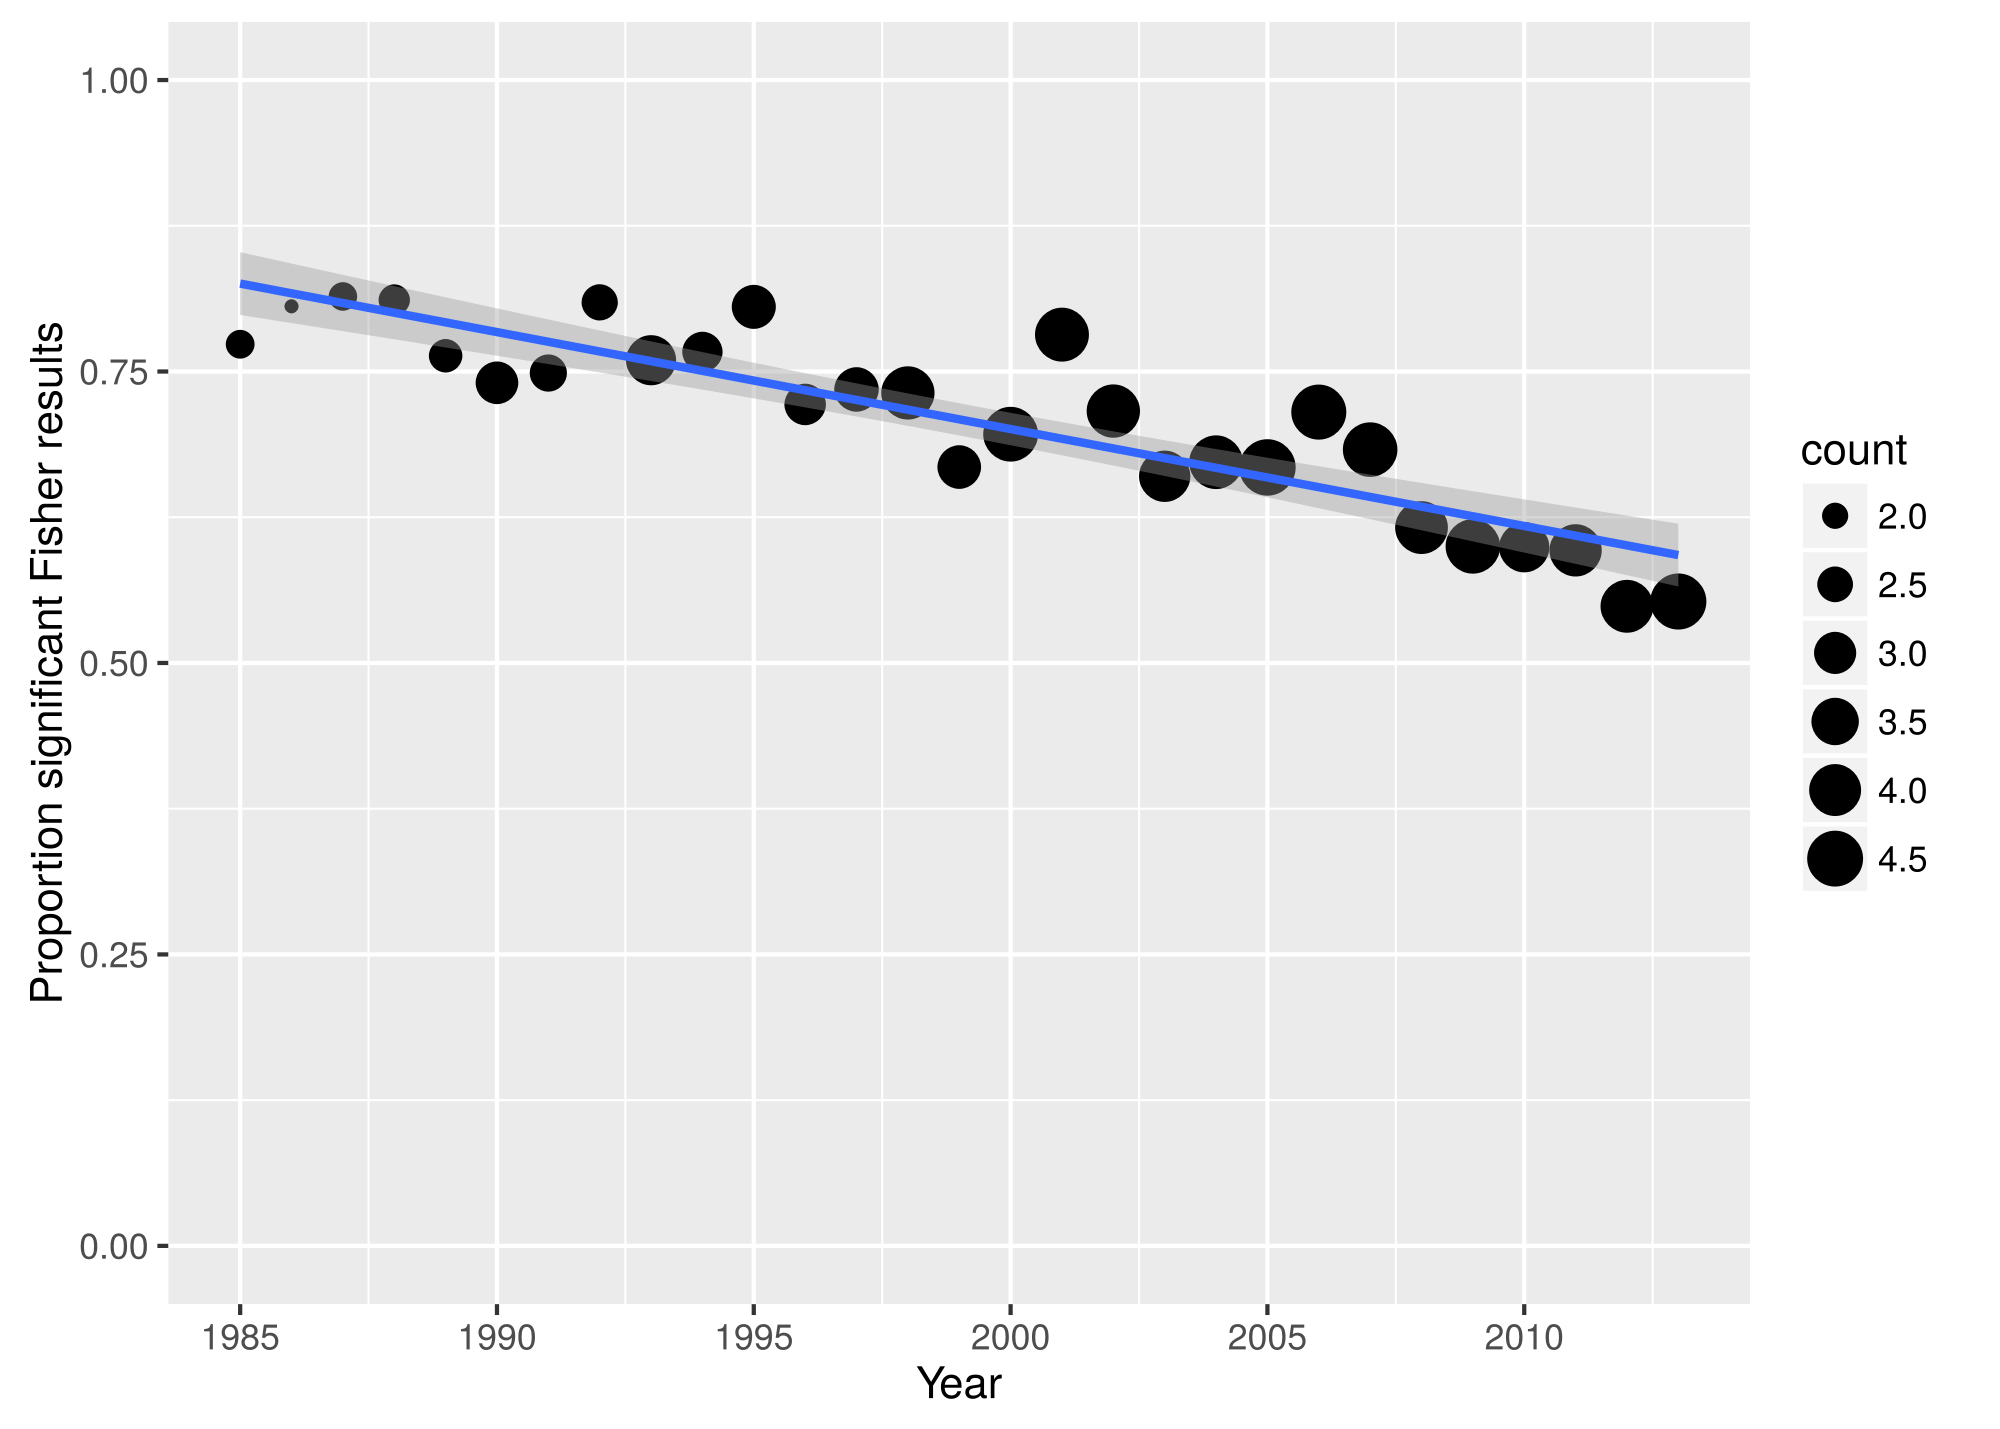
\includegraphics[width=1\linewidth]{assets/figures/tgtbf-fig4.pdf.svg} 

}

\caption{Proportion of papers reporting nonsignificant results in a given year, showing evidence for false negative results. Larger point size indicates a higher mean number of nonsignificant results reported in that year.}\label{fig:tgtbf-fig4}
\end{figure}

\begin{figure}[h]

{\centering 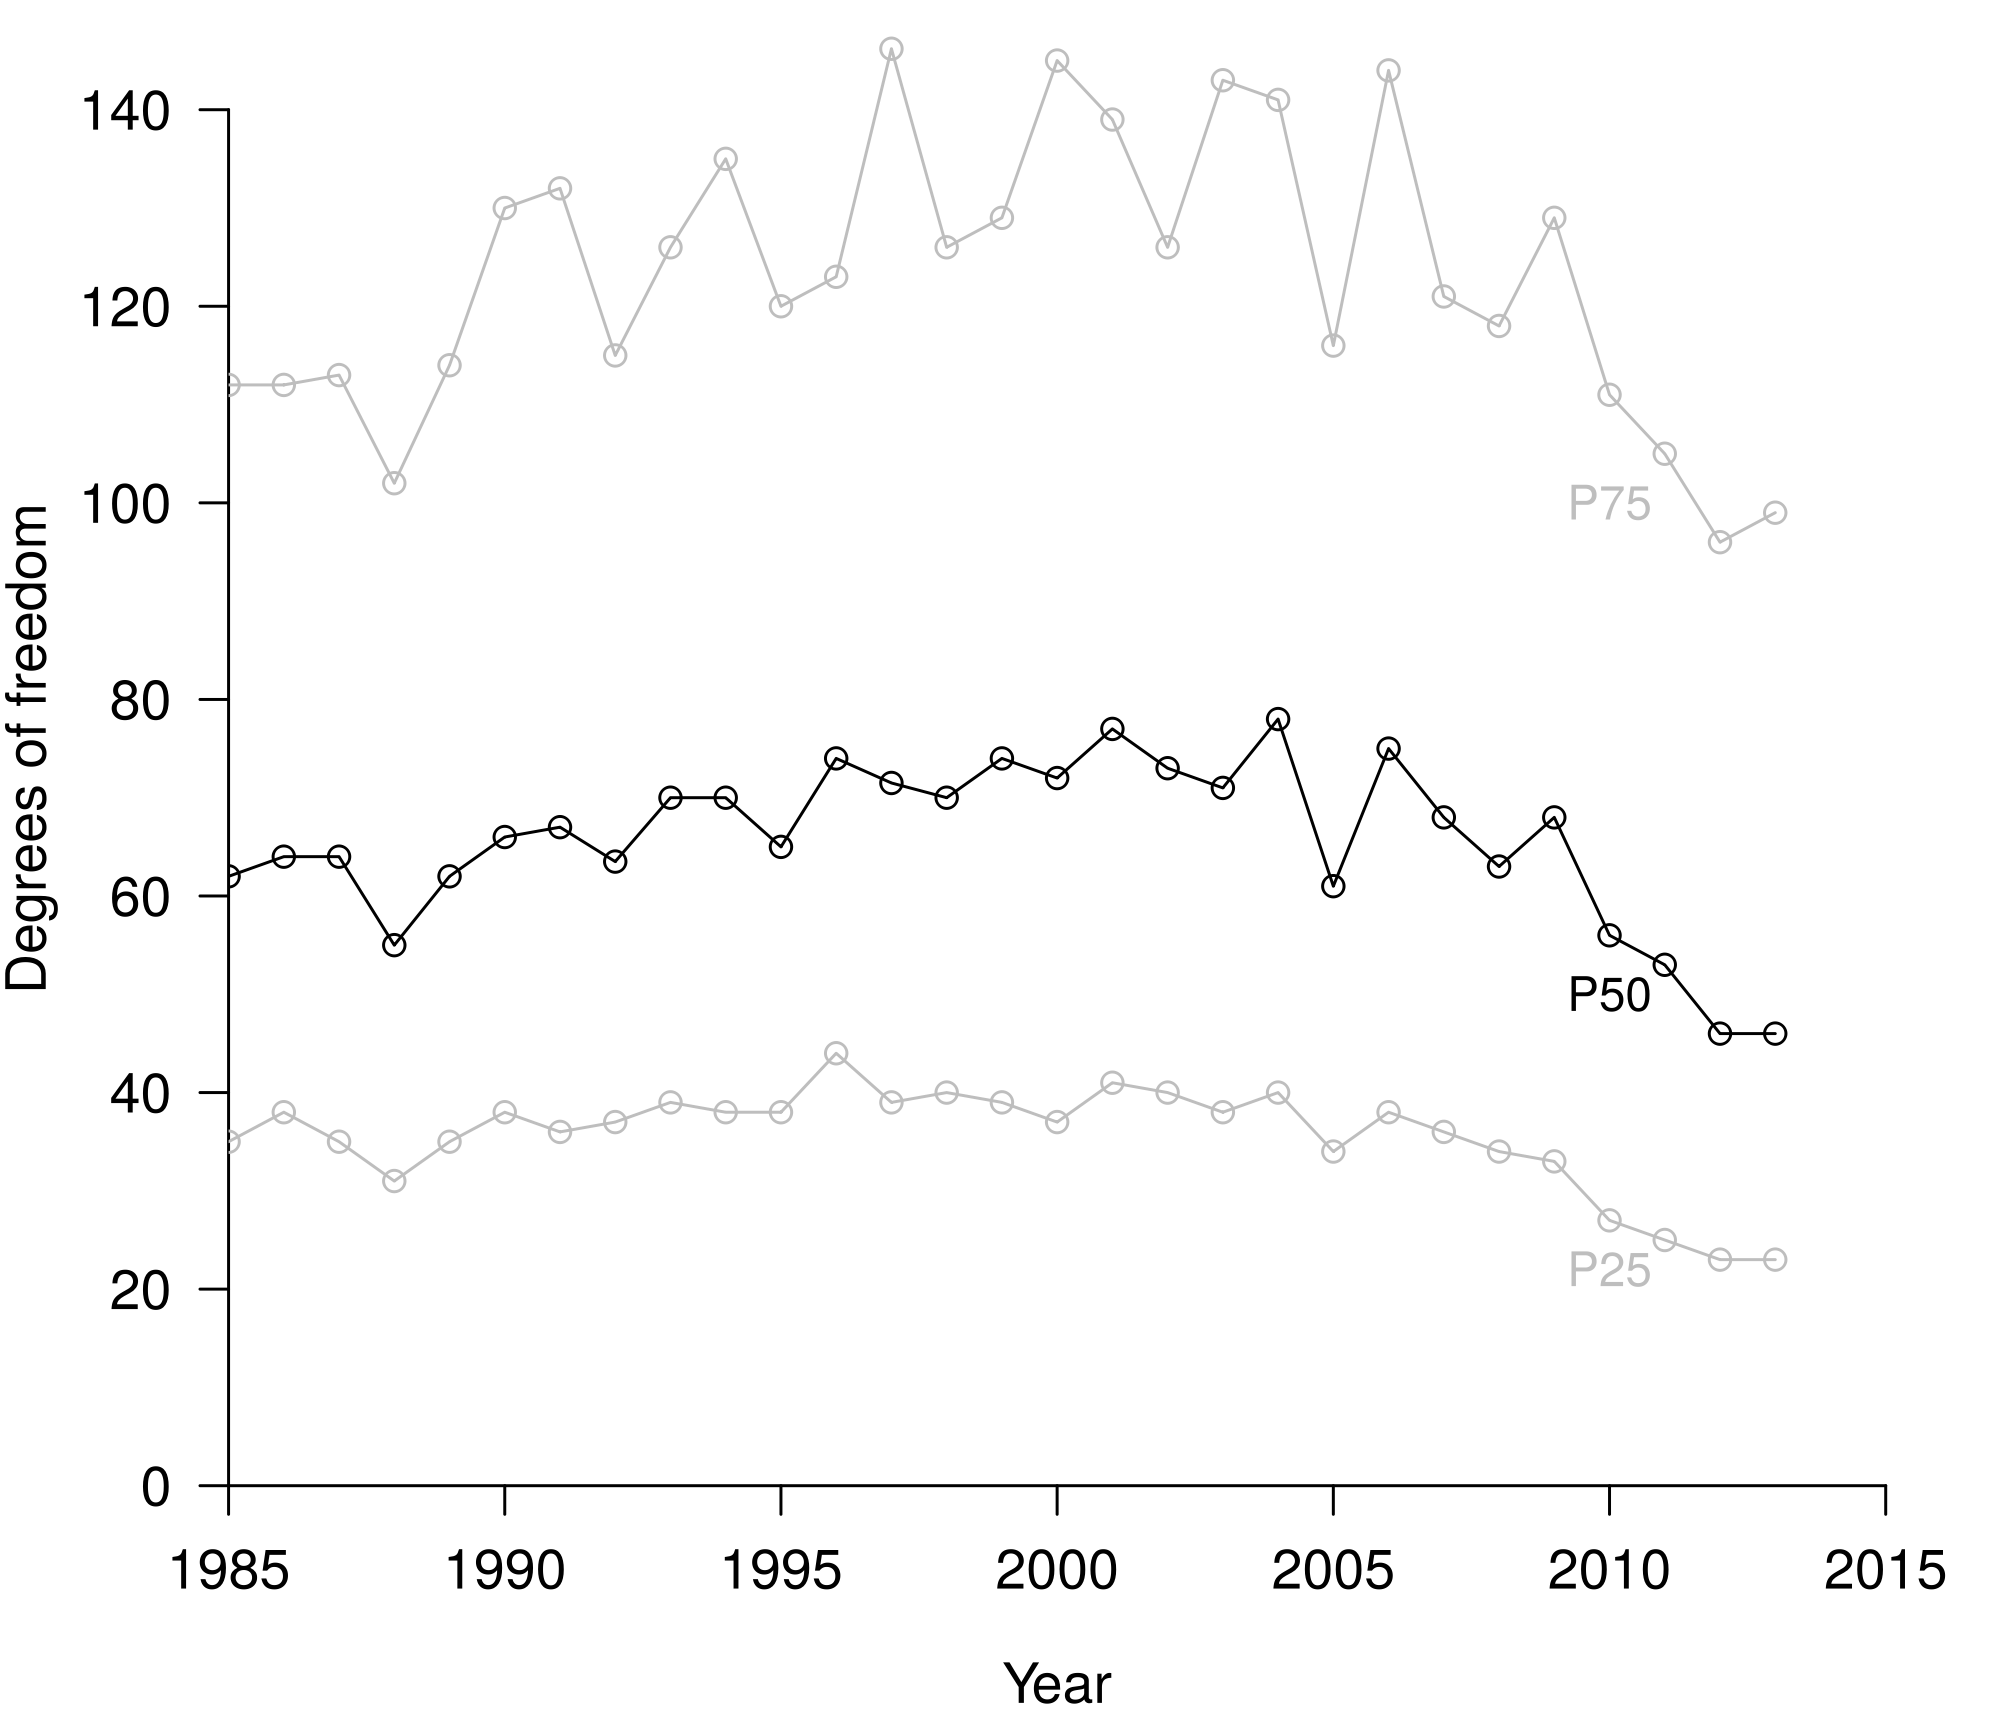
\includegraphics[width=1\linewidth]{assets/figures/tgtbf-fig5.pdf.svg} 

}

\caption{Sample size development in psychology throughout 1985-2013, based on degrees of freedom across 258,050 test results. P25 = 25th percentile. P50 = 50th percentile (i.e., median). P75 = 75th percentile.}\label{fig:tgtbf-fig5}
\end{figure}

\subsection{Discussion}\label{discussion-1}

The result that 2 out of 3 papers containing nonsignificant results show
evidence of at least one false negative empirically verifies previously
voiced concerns about insufficient attention for false negatives
(Fiedler, Kutzner, and Krueger
\protect\hyperlink{ref-doi:10.1177ux2f1745691612462587}{2012}). The
Fisher test proved a powerful test to inspect for false negatives in our
simulation study, where three nonsignificant results already results in
high power to detect evidence of a false negative if sample size is at
least 33 per result and the population effect is medium. Journals
differed in the proportion of papers that showed evidence of false
negatives, but this was largely due to differences in the number of
nonsignificant results reported in these papers. More generally, we
observed that more nonsignificant results were reported in 2013 than in
1985.

The repeated concern about power and false negatives throughout the last
decades seems not to have trickled down into substantial change in
psychology research practice. Cohen
(\protect\hyperlink{ref-doi:10.1037ux2fh0045186}{1962}) and Sedlmeier
and Gigerenzer
(\protect\hyperlink{ref-doi:10.1037ux2f0033-2909.105.2.309}{1989})
already voiced concern decades ago and showed that power in psychology
was low. Fiedler, Kutzner, and Krueger
(\protect\hyperlink{ref-doi:10.1177ux2f1745691612462587}{2012})
contended that false negatives are harder to detect in the current
scientific system and therefore warrant more concern. Despite
recommendations of increasing power by increasing sample size, we found
no evidence for increased sample size (see Figure \ref{fig:tgtbf-fig5}).
To the contrary, the data indicate that average sample sizes have been
remarkably stable since 1985, despite the improved ease of collecting
participants with data collection tools such as online services.

However, what has changed is the amount of nonsignificant results
reported in the literature. Our data show that more nonsignificant
results are reported throughout the years (see Figure
\ref{fig:tgtbf-fig2}), which seems contrary to findings that indicate
that relatively more significant results are being reported (Fanelli
\protect\hyperlink{ref-doi:10.1007ux2fs11192-011-0494-7}{2011};
Sterling, Rosenbaum, and Weinkam
\protect\hyperlink{ref-doi:10.2307ux2f2684823}{1995}; Sterling
\protect\hyperlink{ref-doi:10.2307ux2f2282137}{1959}; De Winter and
Dodou \protect\hyperlink{ref-doi:10.7717ux2fpeerj.733}{2015}). It would
seem the field is not shying away from publishing negative results per
se, as proposed before (Fanelli
\protect\hyperlink{ref-doi:10.1007ux2fs11192-011-0494-7}{2011};
Greenwald \protect\hyperlink{ref-doi:10.1037ux2fh0076157}{1975}; Nosek,
Spies, and Motyl
\protect\hyperlink{ref-doi:10.1177ux2f1745691612459058}{2012}; Rosenthal
\protect\hyperlink{ref-doi:10.1037ux2f0033-2909.86.3.638}{1979};
Schimmack \protect\hyperlink{ref-doi:10.1037ux2fa0029487}{2012}), but
whether this is also the case for results relating to hypotheses of
explicit interest in a study and not all results reported in a paper,
requires further research. Other research strongly suggests that most
reported results relating to hypotheses of explicit interest are
statistically significant (Open Science Collaboration
\protect\hyperlink{ref-doi:10.1126ux2fscience.aac4716}{2015}).

\section{Application 2: Evidence of false negative gender effects in
eight major psychology
journals}\label{application-2-evidence-of-false-negative-gender-effects-in-eight-major-psychology-journals}

In order to illustrate the practical value of the Fisher test to test
for evidential value of (non)significant \(p\)-values, we investigated
gender related effects in a random subsample of our database. Gender
effects are particularly interesting because gender is typically a
control variable and not the primary focus of studies. Hence, we expect
little \(p\)-hacking and substantial evidence of false negatives in
reported gender effects in psychology. We apply the Fisher test to
significant and nonsignificant gender results to test for evidential
value (Van Assen, Van Aert, and Wicherts
\protect\hyperlink{ref-doi:10.1037ux2fmet0000025}{2015}; Simonsohn,
Nelson, and Simmons
\protect\hyperlink{ref-doi:10.1037ux2fa0033242}{2014}). More precisely,
we investigate whether evidential value depends on whether or not the
result is statistically significant, and whether or not the results were
in line with expectations expressed in the paper.

\subsection{Method}\label{method-1}

We planned to test for evidential value in six categories (expectation
{[}3 levels{]} \(\times\) significance {[}2 levels{]}). Expectations
were specified as \enquote{\(H_1\) expected}, \enquote{\(H_0\)
expected}, or \enquote{no expectation}. Prior to data collection, we
assessed the required sample size for the Fisher test based on research
on the gender similarities hypothesis (Hyde
\protect\hyperlink{ref-doi:10.1037ux2f0003-066x.60.6.581}{2005}). We
calculated that the required number of statistical results for the
Fisher test, given \(r=.11\) (Hyde
\protect\hyperlink{ref-doi:10.1037ux2f0003-066x.60.6.581}{2005}) and
80\% power, is 15 \(p\)-values per condition, requiring 90 results in
total. However, the six categories are unlikely to occur equally
throughout the literature, hence we sampled 90 significant and 90
nonsignificant results pertaining to gender, with an expected cell size
of 30 if results are equally distributed across the six cells of our
design. Significance was coded based on the reported \(p\)-value, where
\(\leq.05\) was used as the decision criterion to determine significance
(Nuijten, Hartgerink, et al.
\protect\hyperlink{ref-doi:10.3758ux2fs13428-015-0664-2}{2015}).

We sampled the 180 gender results from our database of over 250,000 test
results in four steps. First, we automatically searched for
\enquote{gender}, \enquote{sex}, \enquote{female} AND \enquote{male}, "
man" AND " woman" {[}sic{]}, or " men" AND " women" {[}sic{]} in the
\(100\) characters before the statistical result and \(100\) after the
statistical result (i.e., range of \(200\) characters surrounding the
result), which yielded 27,523 results. Second, the first author
inspected \(500\) characters before and after the first result of a
randomly ordered list of all 27,523 results and coded whether it indeed
pertained to gender. This was done until 180 results pertaining to
gender were retrieved from 180 different articles. Third, these results
were independently coded by all authors with respect to the expectations
of the original researcher(s) (coding scheme available at
\url{https://osf.io/9ev63}). The coding included checks for qualifiers
pertaining to the expectation of the statistical result
(confirmed/theorized/hypothesized/expected/etc.). If researchers
reported such a qualifier, we assumed they correctly represented these
expectations with respect to the statistical significance of the result.
For example, if the text stated \enquote{as expected no evidence for an
effect was found, \(t(12)=1, p=.337\)} we assumed the authors expected a
nonsignificant result. Fourth, discrepant codings were resolved by
discussion (25 cases {[}13.9\%{]}; two cases remained unresolved and
were dropped). 178 valid results remained for analysis.

Prior to analyzing these 178 \(p\)-values for evidential value with the
Fisher test, we transformed them to variables ranging from 0 to 1.
Statistically nonsignificant results were transformed with Equation
\eqref{eq:pistar}; statistically significant \(p\)-values were divided by
alpha .05 (Van Assen, Van Aert, and Wicherts
\protect\hyperlink{ref-doi:10.1037ux2fmet0000025}{2015}; Simonsohn,
Nelson, and Simmons
\protect\hyperlink{ref-doi:10.1037ux2fa0033242}{2014}).

\subsection{Results}\label{results-1}

The coding of the 178 results indicated that results rarely specify
whether these are in line with the hypothesized effect (see Table
\ref{tab:tgtbf-tab5}. For the 178 results, only 15 clearly stated
whether their results were as expected, whereas the remaining 163 did
not. Illustrative of the lack of clarity in expectations is the
following quote: \enquote{\emph{As predicted, there was little gender
difference {[}\ldots{}{]} p \textless{} .06.}} There were two results
that were presented as significant but contained \(p\)-values larger
than .05; these two were dropped (i.e., 176 results were analyzed). As a
result, the conditions significant-\(H_0\) expected,
nonsignificant-\(H_0\) expected, and nonsignificant-\(H_1\) expected
contained too few results for meaningful investigation of evidential
value (i.e., with sufficient statistical power).

\begin{table}[!h]

\caption{\label{tab:tgtbf-tab5}Number of gender results coded per condition in a 2 (significance: significant or nonsignificant) by 3 (expectation: $H_0$ expected, $H_1$ expected, or no expectation) design. Cells printed in bold had sufficient results to inspect for evidential value.}
\centering
\begin{tabular}{lrll}
\toprule
 & $H_0$ expected & $H_1$ expected & No expectation\\
\midrule
\rowcolor{gray!6}  Significant & 0 & \textbf{11} & \textbf{75}\\
Nonsignificant & 2 & 1 & \textbf{87}\\
\bottomrule
\end{tabular}
\end{table}

Figure \ref{fig:tgtbf-fig6} presents the distributions of both
transformed significant and non-significant \(p\)-values. For
significant results, applying the Fisher test to the \(p\)-values showed
evidential value for a gender effect both when an effect was expected
(\(\chi^2(22)=358.904\), \(p<.001\)) and when no expectation was
presented at all (\(\chi^2(15)=1094.911\), \(p<.001\)). Similarly,
applying the Fisher test to nonsignificant gender results without stated
expectation yielded evidence of at least one false negative
(\(\chi^2(174)=324.374\), \(p<.001\)). Unfortunately, we could not
examine whether evidential value of gender effects is dependent on the
hypothesis/expectation of the researcher, because these effects are most
frequently reported without stated expectations.

\begin{figure}[h]

{\centering 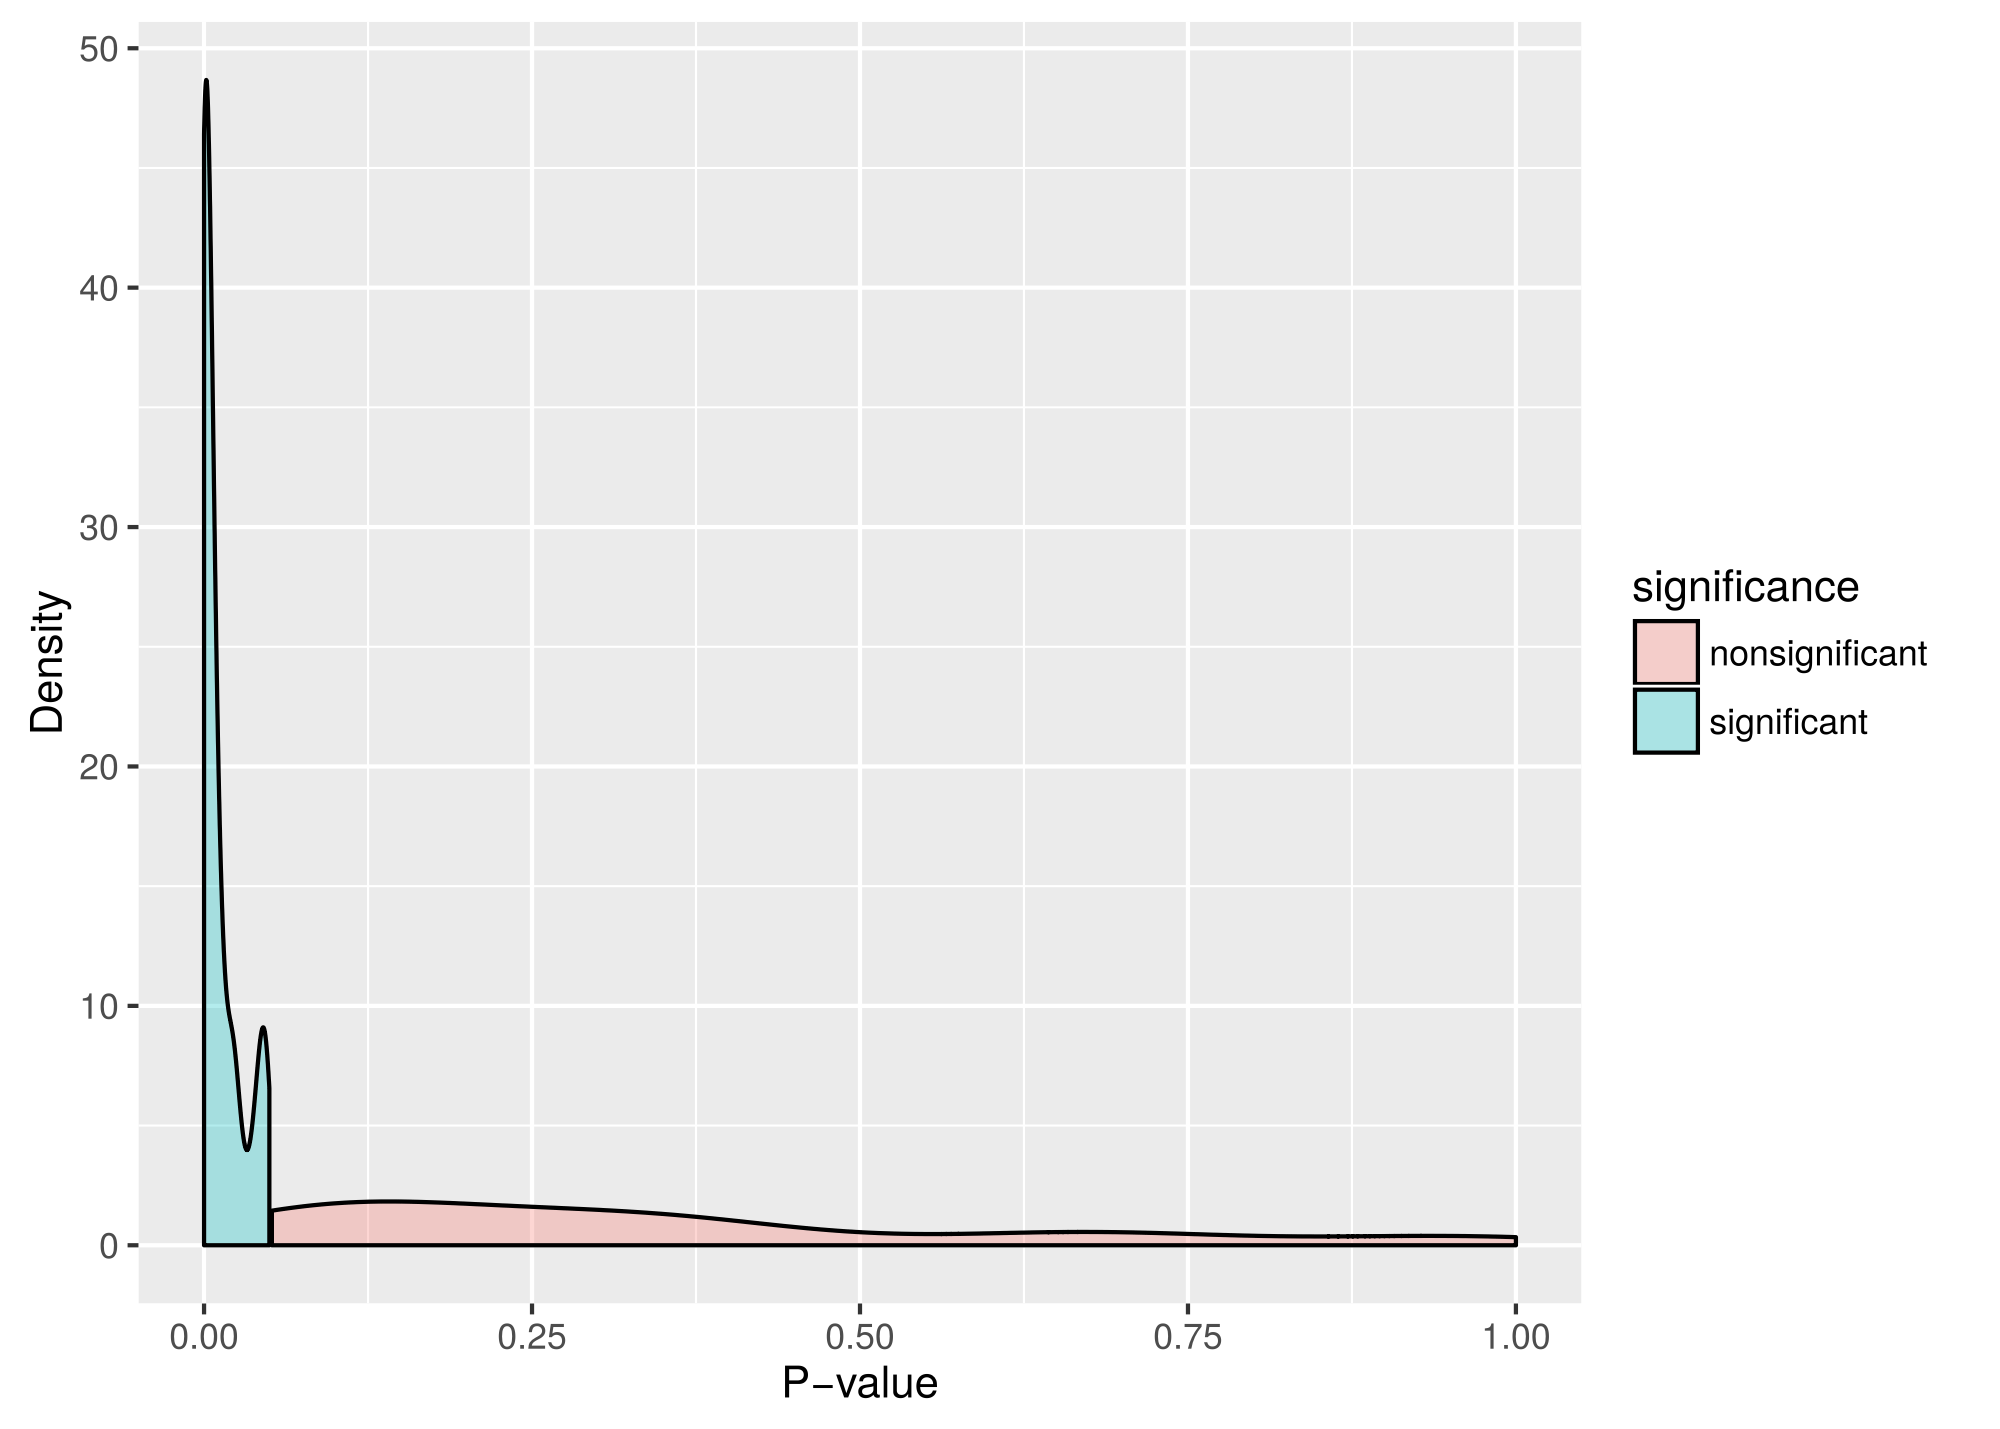
\includegraphics[width=1\linewidth]{assets/figures/tgtbf-fig6.pdf.svg} 

}

\caption{Probability density distributions of the $p$-values for gender effects, split for nonsignificant and significant results. A uniform density distribution indicates the absence of a true effect.}\label{fig:tgtbf-fig6}
\end{figure}

\subsection{Discussion}\label{discussion-2}

We observed evidential value of gender effects both in the statistically
significant (no expectation or \(H_1\) expected) and nonsignificant
results (no expectation). The data from the 178 results we investigated
indicated that in only 15 cases the expectation of the test result was
clearly explicated. This indicates that based on test results alone, it
is very difficult to differentiate between results that relate to a
priori hypotheses and results that are of an exploratory nature. The
importance of being able to differentiate between confirmatory and
exploratory results has been previously demonstrated (Wagenmakers et al.
\protect\hyperlink{ref-doi:10.1177ux2f1745691612463078}{2012}) and has
been incorporated into the Transparency and Openness Promotion
guidelines (TOP; Nosek et al.
\protect\hyperlink{ref-doi:10.1126ux2fscience.aab2374}{2015}) with
explicit attention paid to pre-registration.

\section{Application 3: Reproducibility Project
Psychology}\label{application-3-reproducibility-project-psychology}

Out of the 100 replicated studies in the RPP, 64 did not yield a
statistically significant effect size, despite the fact that high
replication power was one of the aims of the project (Open Science
Collaboration
\protect\hyperlink{ref-doi:10.1126ux2fscience.aac4716}{2015}).
Regardless, the authors suggested \enquote{\emph{\ldots{}that at least
one replication could be a false negative}} (p.~aac4716-4). Here we
estimate how many of these nonsignificant replications might be false
negative, by applying the Fisher test to these nonsignificant effects.

\subsection{Method}\label{method-2}

Of the 64 nonsignificant studies in the RPP data
(\url{https://osf.io/fgjvw}), we selected the 63 nonsignificant studies
with a test statistic. We eliminated one result because it was a
regression coefficient that could not be used in the following
procedure. We first applied the Fisher test to the nonsignificant
results, after transforming them to variables ranging from 0 to 1 using
equations \eqref{eq:pistar} and \eqref{eq:fishertest}. Denote the value of
this Fisher test by \(Y\); note that under the \(H_0\) of no evidential
value \(Y\) is \(\chi^2\)-distributed with 126 degrees of freedom.

Subsequently, we hypothesized that \(X\) out of these 63 nonsignificant
results had a weak, medium, or strong population effect size (i.e.,
\(\rho=.1\), \(.3\), \(.5\), respectively; Cohen
\protect\hyperlink{ref-isbn:9780805802832}{1988}) and the remaining
\(63-X\) had a zero population effect size. For each of these
hypotheses, we generated 10,000 data sets (see next paragraph for
details) and used them to approximate the distribution of the Fisher
test statistic (i.e., \(Y\)). Using this distribution, we computed the
probability that a \(\chi^2\)-value exceeds \(Y\), further denoted by
\(p_Y\). We then used the inversion method (Casella and Berger
\protect\hyperlink{ref-isbn:9780534243128}{2001}) to compute confidence
intervals of \(X\), the number of nonzero effects. Specifically, the
confidence interval for \(X\) is (\(X_{LB};X_{UB}\)), where \(X_{LB}\)
is the value of \(X\) for which \(p_Y\) is closest to \(.025\) and
\(X_{UB}\) is the value of \(X\) for which \(p_Y\) is closest to
\(.975\). We computed three confidence intervals of \(X\): one for the
number of weak, medium, and large effects.

We computed \(p_Y\) for a combination of a value of \(X\) and a true
effect size using 10,000 randomly generated datasets, in three steps.
For each dataset we: + Randomly selected \(X\) out of 63 effects which
are supposed to be generated by true nonzero effects, with the remaining
\(63-X\) supposed to be generated by true zero effects; + Given the
degrees of freedom of the effects, we randomly generated \(p\)-values
under the \(H_0\) using the central distributions and non-central
distributions (for the \(63-X\) and \(X\) effects selected in step 1,
respectively); + The Fisher statistic \(Y\) was computed by applying
Equation (5.2) to the transformed \(p\)-values (see Equation (5.1)) of
step 2. Probability \(p_Y\) equals the proportion of 10,000 datasets
with \(Y\) exceeding the value of the Fisher statistic applied to the
RPP data. See \href{https://osf.io/egnh9}{osf.io/egnh9} for the analysis
script to compute the confidence intervals of \(X\).

\subsection{Results}\label{results-2}

Upon reanalysis of the 63 statistically nonsignificant replications
within RPP we determined that many of these \enquote{failed}
replications say hardly anything about whether there are truly no
effects when using the adapted Fisher method. The Fisher test of these
63 nonsignificant results indicated some evidence for the presence of at
least one false negative finding (\(\chi^2(126)=155.2382\),
\(p=0.039\)). Assuming \(X\) small nonzero true effects among the
nonsignificant results yields a confidence interval of 0-63 (0-100\%).
More specifically, if all results are in fact true negatives then
\(p_Y=.039\), whereas if all true effects are \(\rho=.1\) then
\(p_Y=.872\). Hence, the 63 statistically nonsignificant results of the
RPP are in line with any number of true small effects --- from none to
all. Consequently, we cannot draw firm conclusions about the state of
the field psychology concerning the frequency of false negatives using
the RPP results and the Fisher test, when all true effects are small.
Assuming \(X\) medium or strong true effects underlying the
nonsignificant results from RPP yields confidence intervals 0-21
(0-33.3\%) and 0-13 (0-20.6\%), respectively. In other words, the 63
statistically nonsignificant RPP results are also in line with some true
effects actually being medium or even large.

\subsection{Discussion}\label{discussion-3}

The reanalysis of the nonsignificant RPP results using the Fisher method
demonstrates that any conclusions on the validity of individual effects
based on \enquote{failed} replications, as determined by statistical
significance, is unwarranted. This was also noted by both the original
RPP team (Open Science Collaboration
\protect\hyperlink{ref-doi:10.1126ux2fscience.aac4716}{2015}; Anderson
et al. \protect\hyperlink{ref-doi:10.1126ux2fscience.aad9163}{2016}) and
in a critique of the RPP (Gilbert et al.
\protect\hyperlink{ref-doi:10.1126ux2fscience.aad7243}{2016}).
Replication efforts such as the RPP or the Many Labs project remove
publication bias and result in a less biased assessment of the true
effect size. Nonetheless, single replications should not be seen as the
definitive result, considering that these results indicate there remains
much uncertainty about whether a nonsignificant result is a true
negative or a false negative. The explanation of this finding is that
most of the RPP replications, although often statistically more powerful
than the original studies, still did not have enough statistical power
to distinguish a true small effect from a true zero effect (Maxwell,
Lau, and Howard \protect\hyperlink{ref-doi:10.1037ux2fa0039400}{2015}).
Interpreting results of replications should therefore also take the
precision of the estimate of both the original and replication into
account (Cumming
\protect\hyperlink{ref-doi:10.1177ux2f0956797613504966}{2013}) and
publication bias of the original studies (Etz and Vandekerckhove
\protect\hyperlink{ref-doi:10.1371ux2fjournal.pone.0149794}{2016}).

Very recently four statistical papers have re-analyzed the RPP results
to either estimate the frequency of studies testing true zero hypotheses
or to estimate the individual effects examined in the original and
replication study. All four papers account for the possibility of
publication bias in the original study. Johnson et al.
(\protect\hyperlink{ref-doi:10.1080ux2f01621459.2016.1240079}{2016})
estimated a Bayesian statistical model including a distribution of
effect sizes among studies for which the null-hypothesis is false. On
the basis of their analyses they conclude that at least 90\% of
psychology experiments tested negligible true effects. Johnson et al.'s
model as well as our Fisher's test are not useful for estimation and
testing of individual effects examined in original and replication
study. Interpreting results of individual effects should take the
precision of the estimate of both the original and replication into
account (Cumming
\protect\hyperlink{ref-doi:10.1177ux2f0956797613504966}{2013}). Etz and
Vandekerckhove
(\protect\hyperlink{ref-doi:10.1371ux2fjournal.pone.0149794}{2016})
reanalyzed the RPP at the level of individual effects, using Bayesian
models incorporating publication bias. They concluded that 64\% of
individual studies did not provide strong evidence for either the null
or the alternative hypothesis in either the original of the replication
study. This agrees with our own and Maxwell, Lau, and Howard
(\protect\hyperlink{ref-doi:10.1037ux2fa0039400}{2015}) their
interpretation of the RPP findings. As opposed to Etz and Vandekerckhove
(\protect\hyperlink{ref-doi:10.1371ux2fjournal.pone.0149794}{2016}), Van
Aert and Van Assen
(\protect\hyperlink{ref-doi:10.3758ux2fs13428-017-0967-6}{2017}\protect\hyperlink{ref-doi:10.3758ux2fs13428-017-0967-6}{b})
use a statistically significant original and a replication study to
evaluate the common true underlying effect size, adjusting for
publication bias. From their Bayesian analysis (Van Aert and Van Assen
\protect\hyperlink{ref-doi:10.1371ux2fjournal.pone.0175302}{2017}\protect\hyperlink{ref-doi:10.1371ux2fjournal.pone.0175302}{a})
assuming equally likely zero, small, medium, large true effects, they
conclude that only 13.4\% of individual effects contain substantial
evidence (Bayes factor \textgreater{} 3) of a true zero effect. For a
staggering 62.7\% of individual effects no substantial evidence in favor
zero, small, medium, or large true effect size was obtained. All in all,
conclusions of our analyses using the Fisher are in line with other
statistical papers re-analyzing the RPP data (with the exception of
Johnson et al.
\protect\hyperlink{ref-doi:10.1080ux2f01621459.2016.1240079}{2016})
suggesting that studies in psychology are typically not powerful enough
to distinguish zero from nonzero true findings.

\section{General Discussion}\label{general-discussion}

Much attention has been paid to false positive results in recent years.
Our study demonstrates the importance of paying attention to false
negatives alongside false positives. We examined evidence for false
negatives in nonsignificant results in three different ways.
Specifically, we adapted the Fisher method to detect the presence of at
least one false negative in a set of statistically nonsignificant
results. Simulations indicated the adapted Fisher test to be a powerful
method for that purpose. The three applications indicated that (i)
approximately two out of three psychology articles reporting
nonsignificant results contain evidence for at least one false negative,
(ii) nonsignificant results on gender effects contain evidence of true
nonzero effects, and (iii) the statistically nonsignificant replications
from the Reproducibility Project Psychology (RPP) do not warrant strong
conclusions about the absence or presence of true zero effects
underlying these nonsignificant results (RPP does yield less biased
estimates of the effect; the original studies severely overestimated the
effects of interest).

The methods used in the three different applications provide crucial
context to interpret the results. In applications 1 and 2, we did not
differentiate between main and peripheral results. Hence, the
interpretation of a significant Fisher test result pertains to the
evidence of at least one false negative in all reported results, not the
evidence for at least one false negative in the main results.
Nonetheless, even when we focused only on the main results in
application 3, the Fisher test does not indicate specifically which
result is false negative, rather it only provides evidence for a false
negative in a set of results. As such, the Fisher test is primarily
useful to test a set of potentially underpowered results in a more
powerful manner, albeit that the result then applies to the complete
set. Additionally, in applications 1 and 2 we focused on results
reported in eight psychology journals; extrapolating the results to
other journals might not be warranted given that there might be
substantial differences in the type of results reported in other
journals or fields.

More generally, our results in these three applications confirm that the
problem of false negatives in psychology remains pervasive. Previous
concern about power (Cohen
\protect\hyperlink{ref-doi:10.1037ux2fh0045186}{1962}; Sedlmeier and
Gigerenzer
\protect\hyperlink{ref-doi:10.1037ux2f0033-2909.105.2.309}{1989};
Bakker, Dijk, and Wicherts
\protect\hyperlink{ref-doi:10.1177ux2f1745691612459060}{2012}; Marszalek
et al.
\protect\hyperlink{ref-doi:10.2466ux2f03.11.pms.112.2.331-348}{2011}),
which was even addressed by an APA Statistical Task Force in 1999 that
recommended increased statistical power (Wilkinson
\protect\hyperlink{ref-doi:10.1037ux2f0003-066x.54.8.594}{1999}), seems
not to have resulted in actual change (Marszalek et al.
\protect\hyperlink{ref-doi:10.2466ux2f03.11.pms.112.2.331-348}{2011}).
Potential explanations for this lack of change is that researchers
overestimate statistical power when designing a study for small effects
(Bakker et al.
\protect\hyperlink{ref-doi:10.1177ux2f0956797616647519}{2016}), use
\(p\)-hacking to artificially increase statistical power, and can act
strategically by running multiple underpowered studies rather than one
large powerful study (Bakker, Dijk, and Wicherts
\protect\hyperlink{ref-doi:10.1177ux2f1745691612459060}{2012}). The
effects of \(p\)-hacking are likely to be the most pervasive, with many
people admitting to using such behaviors at some point (John,
Loewenstein, and Prelec
\protect\hyperlink{ref-doi:10.1177ux2f0956797611430953}{2012}) and
publication bias pushing researchers to find statistically significant
results. As such, the problems of false positives, publication bias, and
false negatives are intertwined and mutually reinforcing.

Reducing the emphasis on binary decisions in individual studies and
increasing the emphasis on the precision of a study might help reduce
the problem of decision errors (Cumming
\protect\hyperlink{ref-doi:10.1177ux2f0956797613504966}{2013}). For
example, a large but statistically nonsignificant study might yield a
confidence interval (CI) of the effect size of {[}-0.01; 0.05{]},
whereas a small but significant study might yield a CI of {[}0.01;
1.30{]}. In a purely binary decision mode, the small but significant
study would result in the conclusion that there is an effect because it
provided a statistically significant result, despite it containing much
more uncertainty than the larger study about the underlying true effect
size. In a precision mode, the large study provides a more certain
estimate and therefore is deemed more informative and provides the best
estimate. Using meta-analyses to combine estimates obtained in studies
on the same effect may further increase the overall estimate's
precision. Although the emphasis on precision and the meta-analytic
approach is fruitful in theory, we should realize that publication bias
will result in precise but biased (overestimated) effect size estimation
of meta-analyses (Nuijten, Van Assen, et al.
\protect\hyperlink{ref-doi:10.1037ux2fgpr0000034}{2015}).

\subsection{Limitations and further
research}\label{limitations-and-further-research}

For all three applications, the Fisher tests' conclusions are limited to
detecting at least one false negative in a \emph{set of results}. The
method cannot be used to draw inferences on individuals results in the
set. To draw inferences on the true effect size underlying one specific
observed effect size, generally more information (i.e., studies) is
needed to increase the precision of the effect size estimate.

Another potential caveat relates to the data collected with the
\texttt{R} package \texttt{statcheck} and used in applications 1 and 2.
\texttt{statcheck} extracts inline, APA style reported test statistics,
but does not include results included from tables or results that are
not reported as the APA prescribes. Consequently, our results and
conclusions may not be generalizable to \emph{all} results reported in
articles.

Given that the results indicate that false negatives are still a problem
in psychology, albeit slowly on the decline in published research,
further research is warranted. Further research could focus on comparing
evidence for false negatives in main and peripheral results. Our results
in combination with results of previous studies suggest that publication
bias mainly operates on results of tests of main hypotheses, and less so
on peripheral results. Another venue for future research is using the
Fisher test to re-examine evidence in the literature on certain other
effects or often-used covariates, such as age and race, or to see if it
helps researchers prevent dichotomous thinking with individual
\(p\)-values (Hoekstra et al.
\protect\hyperlink{ref-doi:10.3758ux2fbf03213921}{2006}). Finally, the
Fisher test may and is also used to meta-analyze effect sizes of
different studies. Whereas Fisher used his method to test the
null-hypothesis of an underlying true zero effect using several studies'
\(p\)-values, the method has recently been extended to yield unbiased
effect estimates using only statistically significant \(p\)-values. The
principle of uniformly distributed \(p\)-values given the true effect
size on which the Fisher method is based, also underlies newly developed
methods of meta-analysis that adjust for publication bias, such as
\(p\)-uniform (Van Assen, Van Aert, and Wicherts
\protect\hyperlink{ref-doi:10.1037ux2fmet0000025}{2015}) and \(p\)-curve
(Simonsohn, Nelson, and Simmons
\protect\hyperlink{ref-doi:10.1037ux2fa0033242}{2014}). Extensions of
these methods to include nonsignificant as well as significant
\(p\)-values and to estimate heterogeneity are still under construction.

To conclude, our three applications indicate that false negatives remain
a problem in the psychology literature, despite the decreased attention
and that we should be wary to interpret statistically nonsignificant
results as there being no effect in reality. One way to combat this
interpretation of statistically nonsignificant results is to incorporate
testing for potential false negatives, which the Fisher method
facilitates in a highly approachable manner (a spreadsheet for carrying
out such a test is available at \url{https://osf.io/tk57v/}).

\chapter{688,112 Statistical Results: Content Mining Psychology Articles
for Statistical Test
Results}\label{statistical-results-content-mining-psychology-articles-for-statistical-test-results}

In this chapter, I describe a dataset (available at
\url{http://doi.org/10.17026/dans-2cm-v9j9}) that is the result of
content mining 167,318 published psychology articles for statistical
test results. I tried to mine the content of HTML articles in all
psychology journals published by the six major publishers in psychology,
and succeeded in doing so for four major publishers (see Table
\ref{tab:data-1} for descriptives per publisher). This content mining
was done with the \texttt{R} package \texttt{statcheck} (Nuijten,
Hartgerink, et al.
\protect\hyperlink{ref-doi:10.3758ux2fs13428-015-0664-2}{2015}; Epskamp
and Nuijten \protect\hyperlink{ref-statcheck}{2016}), which extracts
statistical results from research articles in an automated fashion,
given that they are reported in the format prescribed by the American
Psychological Association (APA). I only inspected psychology journals,
because this is a standard within the field of psychology and not
necessarily outside of this field.

\begin{landscape}\begin{table}[t]

\caption{\label{tab:data-1}An overview of the publishers included accompanied by descriptive statistics per publisher regarding the extracted APA results.}
\centering
\resizebox{\linewidth}{!}{
\begin{tabular}{lllllrrr}
\toprule
Publisher & Timespan & \# articles & \# articles with results & \# results & Median \# results per article & Mean reported p-value & Mean recalculated p-value\\
\midrule
\rowcolor{gray!6}  APA & 1985–2016 & 74,489 & 36,662 & 522,367 & 9 & 0.073 & 0.098\\
Sage & 1972–2016 & 13,893 & 5,118 & 59,561 & 8 & 0.101 & 0.110\\
\rowcolor{gray!6}  Springer & 2003–2016 & 53,667 & 8,333 & 97,657 & 8 & 0.097 & 0.113\\
Taylor \& Francis & 2003–2016 & 25,274 & 732 & 8,527 & 8 & 0.118 & 0.133\\
\rowcolor{gray!6}  Total & 1972–2016 & 167,318 & 50,845 & 688,112 & 9 & 0.080 & 0.102\\
\bottomrule
\end{tabular}}
\end{table}
\end{landscape}

The \texttt{statcheck} software extracted 688,112 results from 50,845
articles (out of 167,318 articles). The extracted statistical test
results are presented in long format in this dataset (i.e., each row
corresponds to one statistical result). For each extracted statistical
test result, the reported statistical values are used to recalculate the
\(p\)-value for the reported statistical result. These recalculated
\(p\)-values are checked against the reported \(p\)-value for (decision)
errors. A potential error has occurred when the reported \(p\)-value is
not congruent with the recalculated \(p\)-value, whereas a decision
error (or gross error) occurs when the recalculated \(p\)-value does not
correspond to the reported \(p\)-value and alters the significance of
the result, assuming \(\alpha=0.05\). The results of this comparison are
available in the dataset. The articles for which no results were found
are not included in the dataset (filenames without results available at
\url{https://raw.githubusercontent.com/chartgerink/2016statcheckdata/master/noresult.txt}).

In order to provide a comprehensive dataset, the statistical results are
supplemented with metadata of the original article as available in
CrossRef (\url{https://crossref.org}). These metadata include the
\texttt{doi}, the publisher, the publication year, the journal, the
author names, the author count, and the publication title. Given that
the dataset is in long format, multiple rows can contain duplicate
metadata if multiple results are extracted from the same article.

This dataset of statistical results and accompanying metadata can be
used to inspect if specific papers include potential statistical errors
or for trends in statistical results over time. Articles based on a
similar dataset inspected the degree to which reporting errors occur
(Nuijten, Hartgerink, et al.
\protect\hyperlink{ref-doi:10.3758ux2fs13428-015-0664-2}{2015}), tried
to assess whether such data could be modeled for \(p\)-hacking
(Hartgerink et al.
\protect\hyperlink{ref-doi:10.7717ux2fpeerj.1935}{2016}), and the degree
to which sample sizes and potential false negative results developed
over time (Hartgerink, Wicherts, and Van Assen
\protect\hyperlink{ref-doi:10.1525ux2fcollabra.71}{2017}). This dataset
can be used to replicate these findings and correlate findings with the
available metadata. These data can also be used as baseline data to
identify extreme statistical results in the literature by determining
their percentile score, or to replicate other meta-research. These are
only a few examples, and \enquote{the best thing to do with {[}the{]}
data will be thought of by someone else} (quote from Rufus Pollock).

\section{Data description}\label{data-description}

The data are provided in a comma separated file (CSV) and in
long-format, where each row contains one statistical result. As such,
multiple rows can pertain to the same article and include the same
metadata. This information is provided in duplicate because any other
file format (wide-format or separate files per article) is unfeasible
without increasing the difficulty to reuse the data (e.g., in JSON
format). Given the size of the full dataset (\textgreater{}200MB), a
smaller test dataset is also included to pilot analysis scripts.

For each of the 688,112 results, 20 variables are included, of which
seven pertain to article metadata and 13 pertain to the individual
statistical results. Table \ref{tab:data-2} lists all variables included
in the dataset. Two specific sets of variables are worth explaining
further. First, only \(F\)-values have two degrees of freedom (i.e.,
\(df1\) and \(df2\)). For \(t\)-values, the reported degrees of freedom
are \(df2\), because \(t^2(df)=F(1,df)\). For all other test statistics
that include degrees of freedom, they are included in \(df1\) (i.e.,
\(\chi^2\),\(r\); \(Z\) contains no degrees of freedom). Second, the
variable \texttt{DecisionError} indicates whether an error results in
wrongly concluding statistical significance (report \(p<0.05\) whereas
the recalculated \(p\)-value yields \(p>0.05\), or vice versa). If the
variables \texttt{OneTail} and \texttt{OneTailedInTxt} are \texttt{TRUE}
(see Table \ref{tab:data-2}), a decision error is reverted to
\texttt{FALSE}.

\begin{landscape}\begin{table}[t]

\caption{\label{tab:data-2}Variables included in the dataset and a description of each variable. }
\resizebox{\linewidth}{!}{
\begin{tabular}{lll}
\toprule
Variable & Type & Description\\
\midrule
\rowcolor{gray!6}  Source & Metadata & Digital Object Identifier (DOI) of the article\\
publisher & Metadata & Publisher of the article, as available in CrossRef\\
\rowcolor{gray!6}  year & Metadata & Publication year, as available in CrossRef\\
journal & Metadata & Journal, as available in CrossRef\\
\rowcolor{gray!6}  Statistic & Individual result & Type of statistical test statistic (possible values t,F,r,Z, and Chi2)\\
\addlinespace
df1 & Individual result & First degree of freedom of the test statistic\\
\rowcolor{gray!6}  df2 & Individual result & Second degree of freedom of the test statistic\\
Test.Comparison & Individual result & Sign used in reporting of test statistic (>, <, =)\\
\rowcolor{gray!6}  Value & Individual result & Reported value of the test statistic\\
Reported.Comparison & Individual result & Sign used in reporting of p-value (>, <, =)\\
\addlinespace
\rowcolor{gray!6}  Reported.P.Value & Individual result & Reported p-value\\
Computed & Individual result & Recalculated p-value (two-tailed) based on Statistic and df1, df2\\
\rowcolor{gray!6}  Raw & Individual result & Raw text of extracted statistical result\\
Error & Individual result & Whether the reported p-value differs from recalculated p-value\\
\rowcolor{gray!6}  DecisionError & Individual result & Whether the reported p-value differs from the recalculated p-value AND significance is different (alpha=0.05)\\
\addlinespace
OneTail & Individual result & Whether the result would be correct if the p-value were one-tailed\\
\rowcolor{gray!6}  OneTailedInTxt & Individual result & Whether the article contains “sided”, “tailed”, or “directional”\\
authors & Metadata & Author names, as available in CrossRef\\
\rowcolor{gray!6}  author\_count & Metadata & Number of authors\\
title & Metadata & Title, as available in CrossRef\\
\bottomrule
\end{tabular}}
\end{table}
\end{landscape}

\section{Methods}\label{methods-1}

The data were collected in five steps: (i) collect journal lists; (ii)
spider journal pages for articles; (iii) download articles; (iv) add
article metadata; and (v) mine articles for statistical results. These
five steps are specified below. All code and version history is
available at \url{https://github.com/chartgerink/2016statcheckdata}
(preserved at \url{http://doi.org/10.5281/zenodo.59818}). Figure
\ref{fig:data-fig1} gives a flowchart of the different steps in the data
collection process.

\begin{figure}[h]

{\centering 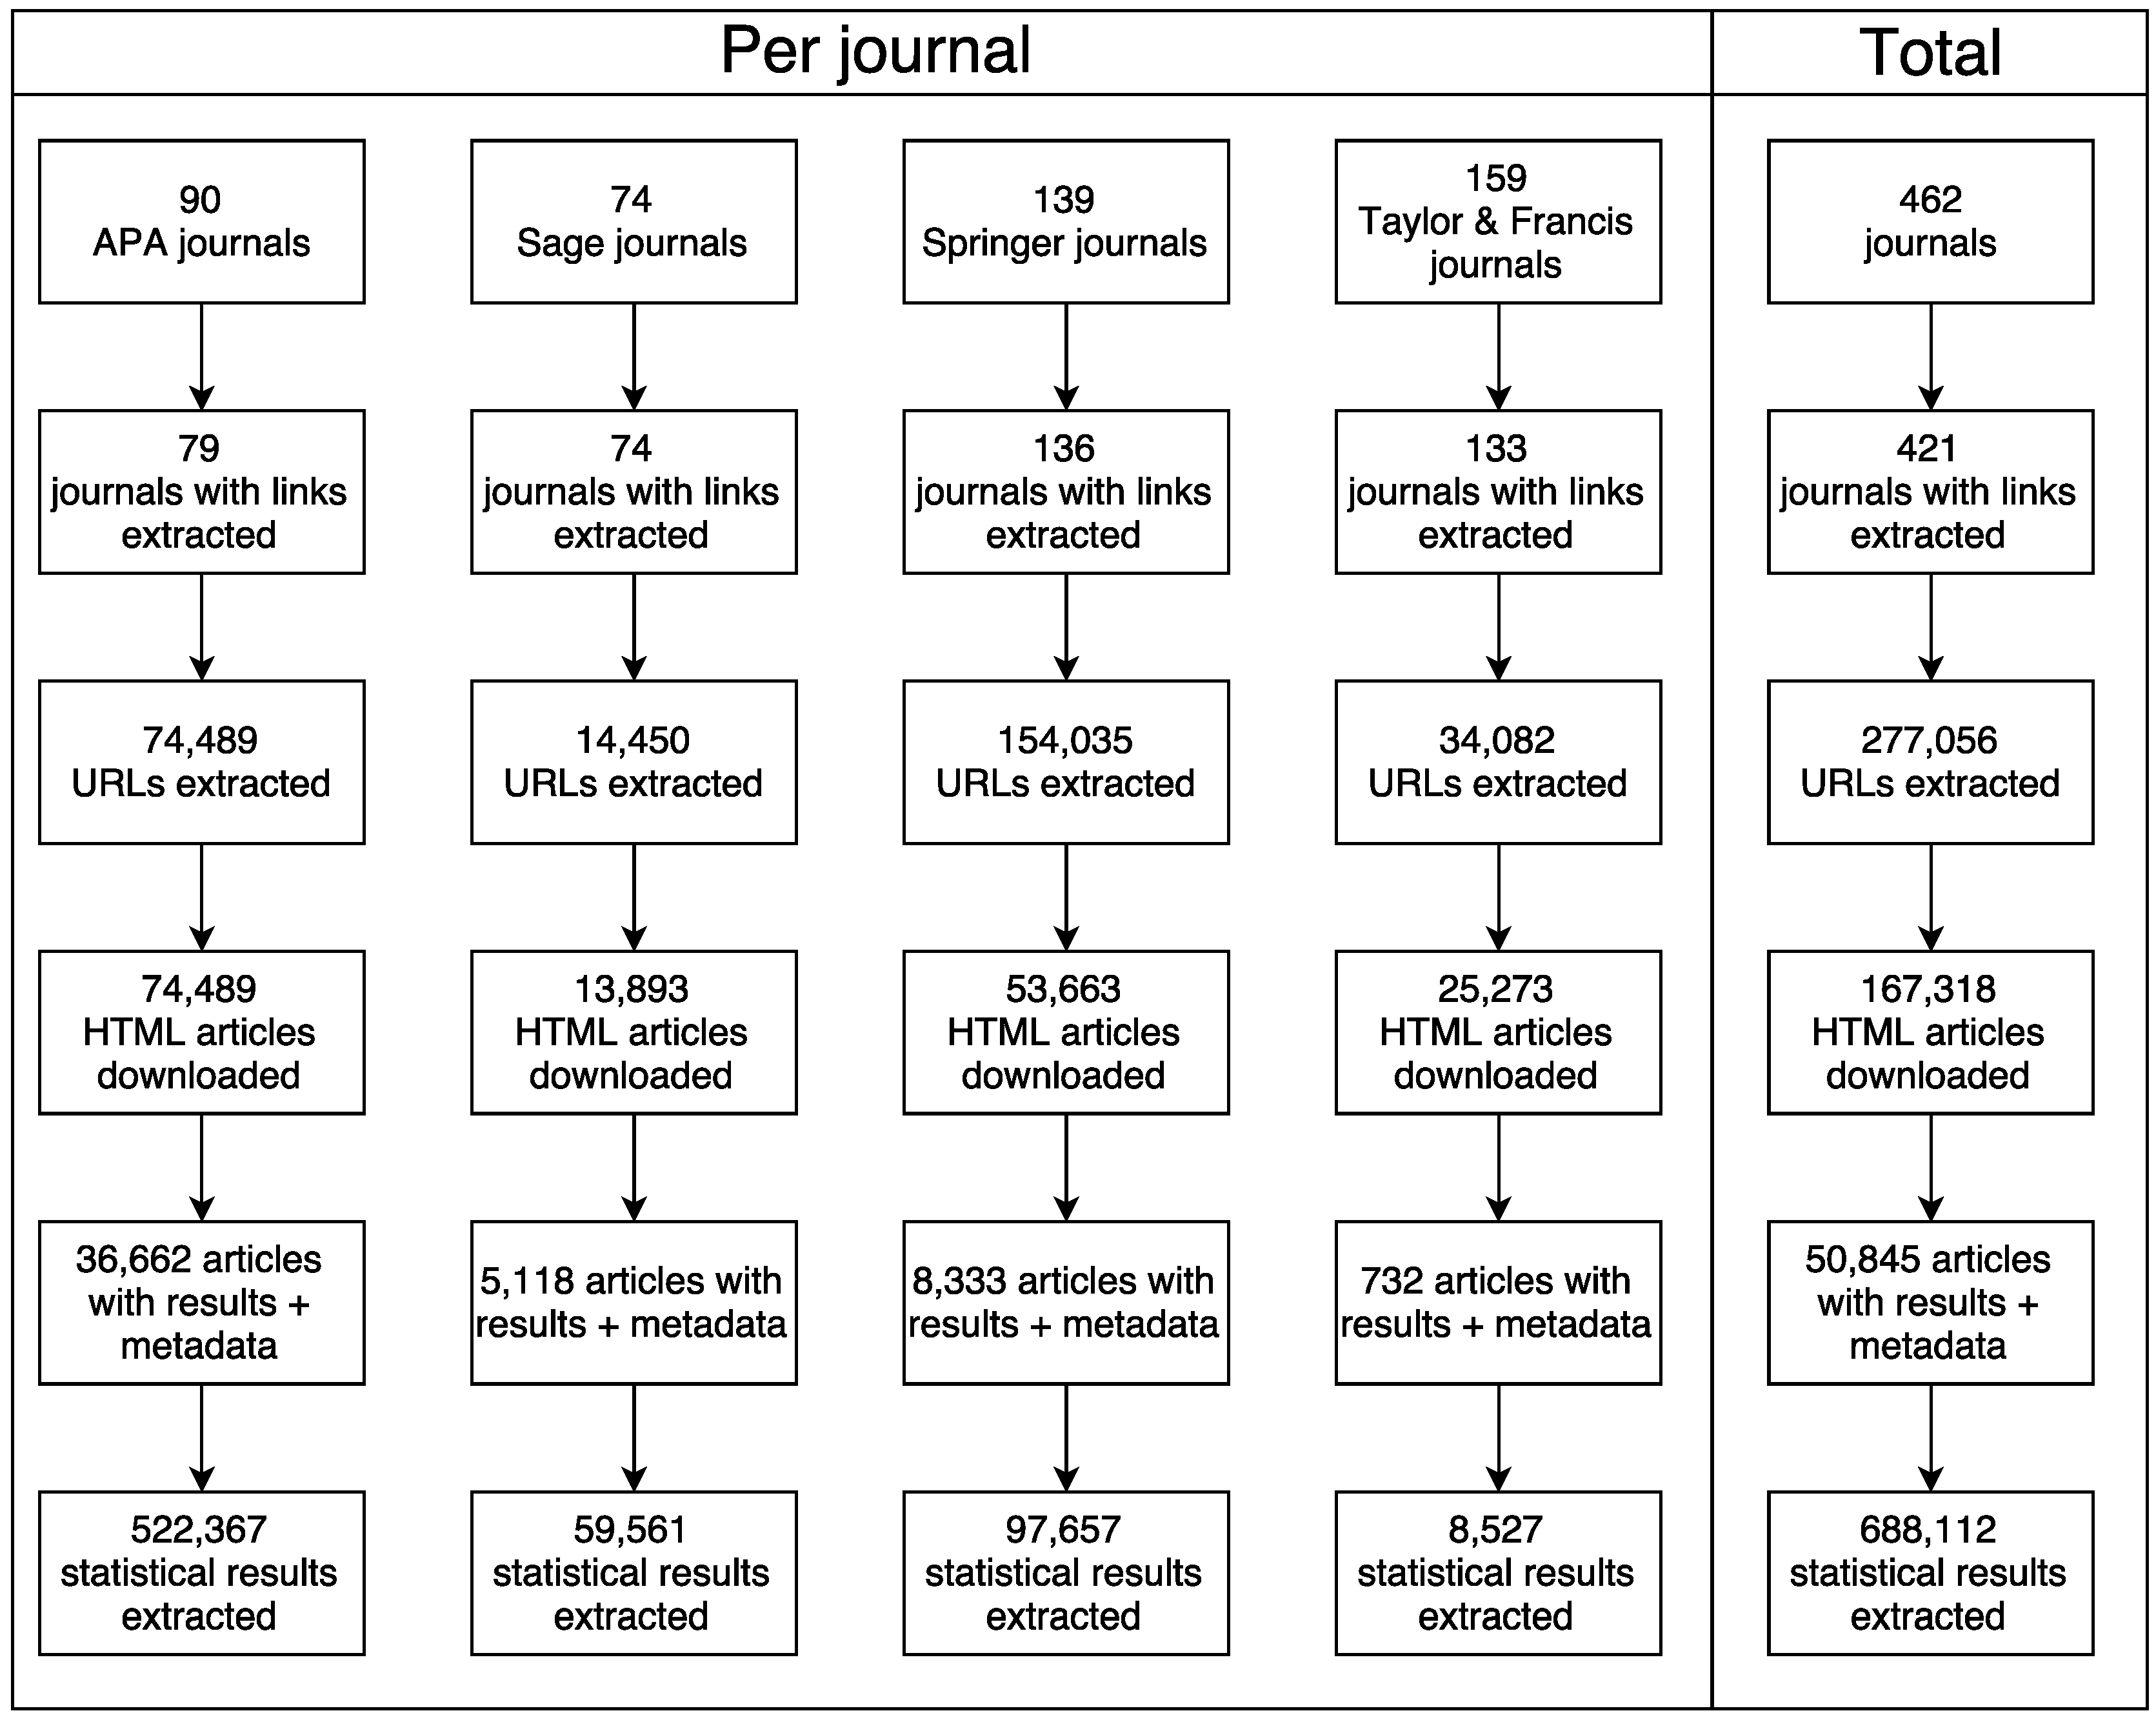
\includegraphics[width=1\linewidth]{assets/figures/statcheck-fig1} 

}

\caption{Flowchart of the data collection process, specified per step in the collection process.}\label{fig:data-fig1}
\end{figure}

Lists of psychology journals from six major publishers were collected
manually. Six publishers were included at the start of this project:
Elsevier, Wiley, Sage, Springer, Taylor \& Francis, and the APA. These
six publishers cover \textgreater{}70\% of the published psychology
literature (Larivière, Haustein, and Mongeon
\protect\hyperlink{ref-doi:10.1371ux2fjournal.pone.0127502}{2015}).
Except for the APA, only journals included in the \enquote{Psychology}
or \enquote{Behavioral Sciences} sections were included (as categorized
by the publishers themselves). These journal lists were collected in
October 2015 and available at
\url{https://github.com/chartgerink/2016statcheckdata/blob/master/scraping/journal-spiders/journallistold.csv}.

Journals from two of the six publishers had to be removed from the
journal list, because Elsevier and Wiley prevented me from automatically
downloading research articles (Hartgerink
\protect\hyperlink{ref-ons-elsevier}{2015}\protect\hyperlink{ref-ons-elsevier}{b};
Bloudoff-Indelicato
\protect\hyperlink{ref-doi:10.1038ux2f527413f}{2015}; Hartgerink
\protect\hyperlink{ref-ons-wiley}{2016}\protect\hyperlink{ref-ons-wiley}{a}).
The library at my university was prompted by these publishers that
suspicious downloading activity occurred, which they thought indicated
compromised user credentials and theft of copyrighted material. The
Tilburg University library services requested me to halt the automated
downloading, in light of potential blocks for the entire university. As
a result, Elsevier and Wiley were excluded from the journal list,
resulting in a remainder of 461 journals from the original 1011 (this
renewed list is available at
\url{https://github.com/chartgerink/2016statcheckdata/blob/master/scraping/journal-spiders/journallist.csv}).

Article URLs were collected with a web spider in April 2016. A web
spider visits a webpage and collects all or a specific set of URLs
included on that webpage. Subsequently, the web spider visits the pages
that are referred to on the initial webpage and again collects URLs,
which it repeats over and over. For this project, a web spider was
developed to extract specific links that referred to full texts
(\url{https://github.com/chartgerink/journal-spiders}). This web spider
produced a set of URLs, which provided direct links to full-text
articles in HTML format (all URLs available at
\url{https://github.com/chartgerink/2016statcheckdata/tree/master/scraping/journal-spiders/journal-links}).
Only those HTMLs that were accessible within the Tilburg University
subscription were collected (list of available journal titles within
subscription available at
\url{https://github.com/chartgerink/2016statcheckdata/blob/master/tilburgjournals.ods?raw=true}).
The original sample, including Elsevier and Wiley, was \(\sim900,000\)
articles.

The research articles were subsequently automatically downloaded, with
the command-line utilities \texttt{wget} (i.e., APA articles) and
\texttt{quickscrape} (v0.4.6
\url{https://github.com/contentmine/quickscrape}; i.e., Sage, Springer,
Taylor \& Francis). This downloading occurred in April--May 2016 and
took into account potential strain on the publisher's servers by
restricting downloads to weekends or limiting the download rate to 10
per minute at most.

Metadata for each article were collected with the Ruby module
\texttt{terrier} (\url{https://github.com/thewinnower/terrier}. This
module queries the CrossRef database when provided with a Digital Object
Identifier (DOI). If available, it returns the available metadata such
as the journal name, publication year, etc. These metadata were
collected in April--June 2016 for all included articles
(\url{https://github.com/chartgerink/2016statcheckdata/blob/master/scraping/terrier.rb}.
Not all articles contained a DOI and no metadata could be collected from
CrossRef as a result.

Finally, after all HTML files were collected and metadata were added,
\texttt{statcheck} (v1.0.1; Nuijten, Hartgerink, et al.
\protect\hyperlink{ref-doi:10.3758ux2fs13428-015-0664-2}{2015}; Epskamp
and Nuijten \protect\hyperlink{ref-statcheck}{2016}) was run in August
2016 to create the final dataset. This \texttt{R} package scans the text
from an article for APA style statistical results, extracts these
statistical results, and checks whether the reported \(p\)-values are
equivalent to the recalculated \(p\)-value (with a margin of error due
to potential rounding). For example, the result \(t(85)=2.86,p=0.005\)
would be automatically extracted. Version 1.0.1 of \texttt{statcheck} is
able to mine \(t\),\(F\),\(r\),\(Z\), and \(\chi^2\) results.

\section{Usage notes}\label{usage-notes}

Usage of the data requires understanding several limitations of the
\texttt{statcheck} package, in order to provide context for results
obtained from this dataset. A manual validity check for
\texttt{statcheck} proved that the software is valid for extracting APA
style reported test results (Nuijten, Hartgerink, et al.
\protect\hyperlink{ref-doi:10.3758ux2fs13428-015-0664-2}{2015}).
However, it does not extract results that are not in line with what the
APA prescribes. Additionally, \texttt{statcheck} only extracts results
reported in the text and not those reported in tabular format or in
images. As such, statistical results from tables and images are
systematically excluded. As a result, any conclusions based on this
dataset should not be extrapolated without caution.

Additionally, it is worth mentioning that relatively few articles
contained results that were extracted by \texttt{statcheck} (\(\sim1/3\)
downloaded articles). This could be due to at least three reasons.
First, results might not be reported according to the APA format in some
psychology journals/volumes, which results in fewer extracted results.
Second, statistical results could be reported in APA format, but these
statistical results are not \(t\),\(F\),\(r\),\(Z\), or \(\chi^2\).
Third, a considerable part of the literature might pertain to
theoretical papers, case studies, or narrative reviews, instead of
empirical research.

The presented data have been deposited in the Dutch Archival Network for
the Sciences (DANS) and are available under a public domain license (CC0
1.0 rights waiver). The DANS repository is a trustworthy digital
repository and has received the Data Seal of Approval (DSA), the World
Data System (WDS) certificate, and the NESTOR-seal. This ensures that
deposited data will remain available for a substantial amount of time.
All rights to this dataset are waived to the furthest extent possible,
such that reuse is maximized.

In addition to preserving the data in the DANS repository, individual
reports have been generated for each of the 50,845 articles and posted
on PubPeer (\url{https://pubpeer.com/}). Appendix C shows a fictitious
example of such a report. These reports were generated in order to
increase the accessibility of the data for those wanting to investigate
a specific paper instead of the entire dataset. Additionally, this
increases the discoverability of potential errors by posting them in a
central forum of post-publication peer review.

\chapter{Detection of data fabrication using statistical
tools}\label{detection-of-data-fabrication-using-statistical-tools}

Any field of empirical inquiry is faced with cases of scientific
misconduct at some point, either in the form of fabrication,
falsification, or plagiarism (FFP). Psychology faced Stapel; medical
sciences faced Poldermans and Macchiarini; life sciences faced Voignet;
physical sciences faced Schön --- these are just a few examples of
research misconduct cases in the last decade. Overall, an estimated 2\%
of all scholars admit to having falsified or fabricated research results
at least once during their career (Fanelli
\protect\hyperlink{ref-doi:10.1371ux2fjournal.pone.0005738}{2009}),
which due to its self-report nature is likely to be an underestimate of
the true rate of misconduct. The detection rate of data fabrication is
likely to be even lower; for example, among several hundreds of
thousands of researchers working in the United States and the
Netherlands, only around a dozen cases become public each year. At best,
this suggests a detection rate below 1\% among those 2\% who admit to
fabricating or falsifying data --- the tip of a seemingly much larger
iceberg.

The ability to detect fabricated data may help deter researchers from
fabricating data in their work. Deterrence theory (e.g., Hobbes
\protect\hyperlink{ref-leviathan}{1651}) states that improved detection
of undesirable behaviors decreases the expected utility of said
behaviors, ultimately leading to fewer people to engage in it. Detection
techniques have developed differently for fabrication, falsification,
and plagiarism. Plagiarism scanners have been around the longest (e.g.,
Parker and Hamblen
\protect\hyperlink{ref-doi:10.1109ux2f13.28038}{1989}) and are widely
implemented in practice, not only at journals but also in the evaluation
of student theses (e.g., with commercial services such as Turnitin).
Various tools have been developed to detect image manipulation and some
of these tools have been implemented at biomedical journals to screen
for fabricated or falsified images. For example, the Journal of Cell
Biology and the EMBO journal scan each submitted image for potential
image manipulation (The Journal of Cell Biology
\protect\hyperlink{ref-The_Journal_of_Cell_Biology2015-vh}{2015}\protect\hyperlink{ref-The_Journal_of_Cell_Biology2015-vh}{b};
Nature editors \protect\hyperlink{ref-doi:10.1038ux2f546575a}{2017}),
which supposedly increases the risk of detecting (blatant) image
manipulation. Recently developed algorithms even allow automated
scanning of images for such manipulations (Koppers, Wormer, and Ickstadt
\protect\hyperlink{ref-doi:10.1007ux2fs11948-016-9841-7}{2016}). The
application of such tools can also help researchers systematically
evaluate research articles in order to estimate the extent to which
image manipulation occurs in the literature (4\% of all papers are
estimated to contain manipulated images; Bik, Casadevall, and Fang
\protect\hyperlink{ref-doi:10.1128ux2fmBio.00809-16}{2016}\protect\hyperlink{ref-doi:10.1128ux2fmBio.00809-16}{b})
and to study factors that predict image manipulation (Fanelli et al.
\protect\hyperlink{ref-doi:10.1007ux2fs11948-018-0023-7}{2018}).

Methods to detect fabrication of quantitative data are often based on a
mix of psychology theory and statistics theory. Because humans are
notoriously bad at understanding and estimating randomness (Haldane
\protect\hyperlink{ref-Haldane1948-nm}{1948}; Tversky and Kahneman
\protect\hyperlink{ref-doi:10.1126ux2fscience.185.4157.1124}{1974};
Tversky and Kahneman
\protect\hyperlink{ref-doi:10.1037ux2fh0031322}{1971}; Nickerson
\protect\hyperlink{ref-doi:10.1037ux2f1082-989X.5.2.241}{2000}; Wagenaar
\protect\hyperlink{ref-doi:10.1037ux2fh0032060}{1972}), they might
create fabricated data that fail to follow the fundamentally
probabilistic nature of genuine data. Data and outcomes of analyses
based on these data that fail to align with the (at least partly
probabilistic) processes that are assumed to underlie genuine data may
indicate deviations from the reported data collecting protocol,
potentially even data fabrication or falsification.

Statistical methods have proven to be of importance in initiating data
fabrication investigations or in assessing the scope of potential data
fabrication. For example, Kranke, Apfel, and Roewer skeptically
perceived Fujii's data (Kranke, Apfel, and Roewer
\protect\hyperlink{ref-doi:10.1213ux2f00000539-200004000-00053}{2000})
and used statistical methods to contextualize their skepticism. At the
time, a reviewer perceived them to be on a \enquote{crusade against
Fujii and his colleagues} (Kranke
\protect\hyperlink{ref-doi:10.1111ux2fj.1365-2044.2012.07318.x}{2012})
and further investigation remained absent. Only when Carlisle extended
the systematic investigation to 168 of Fujii's papers for misconduct
(Carlisle
\protect\hyperlink{ref-doi:10.1111ux2fj.1365-2044.2012.07128.x}{2012};
Carlisle and Loadsman
\protect\hyperlink{ref-doi:10.1111ux2fanae.13650}{2016}; Carlisle et al.
\protect\hyperlink{ref-doi:10.1111ux2fanae.13126}{2015}) did events
cumulate into an investigation- and ultimately retraction of 183 of
Fujii's peer-reviewed papers (Oransky
\protect\hyperlink{ref-oransky2015}{2015}; ``Joint Editors-in-Chief
request for determination regarding papers published by Dr. Yoshitaka
Fujii''
\protect\hyperlink{ref-doi:10.1016ux2fj.ijoa.2012.10.001}{2013}). In
another example, the Stapel case, statistical evaluation of his oeuvre
occurred after he had already confessed to fabricating data, which
ultimately resulted in 58 retractions of papers (co-)authored by Stapel
(Levelt \protect\hyperlink{ref-Levelt2012}{2012}; Oransky
\protect\hyperlink{ref-oransky2015}{2015}).

In order to determine whether the application of statistical methods to
detect data fabrication is responsible and valuable, we need to study
their diagnostic value. Specifically, many of the developed statistical
methods to detect data fabrication are quantifications of case specific
suspicions by researchers, but these applications do not inform us on
their diagnostic value (i.e., sensitivity and specificity) outside of
those specific cases. Side-by-side comparisons of different statistical
methods to detect data fabrication has also been difficult through the
in-casu origin of these methods. Moreover, the efficacy of these methods
based on known cases is likely to be biased, considering that an unknown
amount of undetected cases is not included. Using different statistical
methods to detect fabricated data using genuine versus fabricated data
yields information on the sensitivity and specificity of the detection
tools. This is important because of the severe professional- and
personal consequences of accusations of potential research misconduct
(as illustrated by the STAP case; Cyranoski
\protect\hyperlink{ref-doi:10.1038ux2f520600a}{2015}). These methods
might have utility in misconduct investigations where the prior chances
of misconduct are high, but their diagnostic value in large-scale
applications to screen the literature are unclear.

In this article, we investigate the diagnostic performance of various
statistical methods to detect data fabrication. These statistical
methods (detailed next) have not previously been validated
systematically in research using both genuine and fabricated data. We
present two studies where we try to distinguish (arguably) genuine data
from known fabricated data based on these statistical methods. These
studies investigate methods to detect data fabrication in summary
statistics (Study 1) or in individual level (raw) data (Study 2) in
psychology. In Study 1, we invited researchers to fabricate summary
statistics for a set of four anchoring studies, for which we also had
genuine data from the Many Labs 1 initiative
(\url{https://osf.io/pqf9r}; R. A. Klein et al.
\protect\hyperlink{ref-doi:10.1027ux2f1864-9335ux2fa000178}{2014}). In
Study 2, we invited researchers to fabricate individual level data for a
classic Stroop experiment, for which we also had genuine data from the
Many Labs 3 initiative (\url{https://osf.io/n8xa7/}; Ebersole et al.
\protect\hyperlink{ref-doi:10.1016ux2fj.jesp.2015.10.012}{2016}). Before
presenting these studies, we discuss the theoretical framework of the
investigated statistical methods to detect data fabrication.

\section{Theoretical framework}\label{theoretical-framework-1}

Statistical methods to detect potential data fabrication can be based
either on reported summary statistics that can often be retrieved from
articles or on the raw (underlying) data if these are available. Below
we detail \(p\)-value analysis, variance analysis, and effect size
analysis as potential ways to detect data fabrication using summary
statistics. \(P\)-value analyses can be applied whenever a set of
nonsignificant \(p\)-values are reported; variance analysis can be
applied whenever a set of variances and accompanying sample sizes are
reported for independent, randomly assigned groups; effect size analysis
can be used whenever the effect size is reported or calculated (e.g., an
APA reported t- or F-statistic; Hartgerink, Wicherts, and Van Assen
\protect\hyperlink{ref-doi:10.1525ux2fcollabra.71}{2017}). Among the
methods that can be applied to uncover potential fabrication using raw
data, we consider digit analyses (i.e., the Newcomb-Benford law and
terminal digit analysis) and multivariate associations between
variables. The Newcomb-Benford law can be applied on ratio- or count
scale measures that have sufficient digits and that are not truncated
(Hill and Schürger
\protect\hyperlink{ref-doi:10.1016ux2fj.spa.2005.05.003}{2005});
terminal digit analysis can also be applied whenever measures have
sufficient digits (see also Mosimann, Wiseman, and Edelman
\protect\hyperlink{ref-doi:10.1080ux2f08989629508573866}{1995}).
Multivariate associations can be investigated whenever there are two or
more numerical variables available and data on that same relation is
available from (arguably) genuine data sources.

\subsection{Detecting data fabrication in summary
statistics}\label{detecting-data-fabrication-in-summary-statistics}

\subsubsection{\texorpdfstring{\(P\)-value
analysis}{P-value analysis}}\label{p-value-analysis}

The distribution of a single or a set of independent \(p\)-values is
uniform if the null hypothesis is true, while it is right-skewed if the
alternative hypothesis is true (Fisher
\protect\hyperlink{ref-Fisher1925-jl}{1925}). If the model assumptions
of the underlying process hold, the probability density function of one
\(p\)-value is the result of the population effect size, the precision
of the estimate, and the observed effect size, whose properties carry
over to a set of \(p\)-values if those \(p\)-values are independent.

When assumptions underlying the model used to compute a \(p\)-value are
violated, \(p\)-value distributions can take on a variety of shapes. For
example, when optional stopping (i.e., adding batches of participants
until you have a statistically significant result) occurs and the null
hypothesis is true, \(p\)-values just below .05 become more frequent
(Lakens
\protect\hyperlink{ref-doi:10.1080ux2f17470218.2014.982664}{2015}\protect\hyperlink{ref-doi:10.1080ux2f17470218.2014.982664}{a};
Hartgerink et al.
\protect\hyperlink{ref-doi:10.7717ux2fpeerj.1935}{2016}). However, when
optional stopping occurs under the alternative hypothesis or when other
researcher degrees of freedom are used in an effort to obtain
significance (Simmons, Nelson, and Simonsohn
\protect\hyperlink{ref-doi:10.1177ux2f0956797611417632}{2011}; Wicherts
et al. \protect\hyperlink{ref-doi:10.3389ux2ffpsyg.2016.01832}{2016}), a
right-skewed distribution for significant \(p\)-values can and will
likely still occur (Ulrich and Miller
\protect\hyperlink{ref-doi:10.1037ux2fxge0000086}{2015}; Hartgerink et
al. \protect\hyperlink{ref-doi:10.7717ux2fpeerj.1935}{2016}).

A failure of independent \(p\)-values to be right-skewed or uniformly
distributed (as would be theoretically expected) can indicate potential
data fabrication. For example, in the Fujii case, baseline measurements
of supposed randomly assigned groups later turned out to be fabricated.
When participants are randomly assigned to conditions, measures at
baseline are expected to statistically equivalent between the groups
(i.e., equivalent distributions), hence, produce uniformly distributed
\(p\)-values. However, in the Fujii case, Carlisle observed many large
\(p\)-values, which ultimately led to the identification of potential
data fabrication (Carlisle
\protect\hyperlink{ref-doi:10.1111ux2fj.1365-2044.2012.07128.x}{2012}).
The cause of such large \(p\)-values may be that the effect of
randomness is underappreciated when fabricating statistically
nonsignificant data due to (for example) widespread misunderstanding of
what a \(p\)-value means (Sijtsma, Veldkamp, and Wicherts
\protect\hyperlink{ref-doi:10.1007ux2fs11336-015-9444-2}{2015}; Goodman
\protect\hyperlink{ref-doi:10.1053ux2fj.seminhematol.2008.04.003}{2008}),
which results in groups of data that are too similar conditional on the
null hypothesis of no differences between the groups. As an
illustration, we simulated normal distributed measurements for studies
and their \(t\)-test comparisons in Table \ref{tab:ddfab-tab1}, under
statistically equivalent populations (Set 1). We also fabricated
independent data for equivalent groups, where we fixed the mean and
standard deviation for all studies and subsequently added (too) little
uniform noise to these parameters (Set 2). The expected value of a
uniform \(p\)-value distribution is .5, but the fabricated data from our
illustration have a mean \(p\)-value of 0.956.

\begin{table}[!h]

\caption{\label{tab:ddfab-tab1}Examples of means and standard deviations for a continuous outcome in genuine and fabricated randomized clinical trials. Set 1 is randomly generated data under the null hypothesis of random assignment (assumed to be the genuine process), whereas Set 2 is generated under excessive consistency with equal groups. Each trial condition contains 100 participants. The $p$-values are the result of independent $t$-tests comparing the experimental and control conditions within each respective set of a study.}
\centering
\resizebox{\linewidth}{!}{
\begin{tabular}{lllrllr}
\toprule
\multicolumn{1}{c}{} & \multicolumn{3}{c}{Set 1} & \multicolumn{3}{c}{Set 2} \\
\cmidrule(l{3pt}r{3pt}){2-4} \cmidrule(l{3pt}r{3pt}){5-7}
\multicolumn{1}{c}{} & \multicolumn{1}{c}{Experimental} & \multicolumn{1}{c}{Control} & \multicolumn{1}{c}{} & \multicolumn{1}{c}{Experimental} & \multicolumn{1}{c}{Control} & \multicolumn{1}{c}{} \\
\cmidrule(l{3pt}r{3pt}){2-2} \cmidrule(l{3pt}r{3pt}){3-3} \cmidrule(l{3pt}r{3pt}){5-5} \cmidrule(l{3pt}r{3pt}){6-6}
 & M (SD) & M (SD) & P-value & M (SD) & M (SD) & P-value\\
\midrule
\rowcolor{gray!6}  Study 1 & 48.432 (10.044) & 49.158 (9.138) & 0.594 & 52.274 (10.475) & 63.872 (10.684) & 0.918\\
Study 2 & 50.412 (10.322) & 49.925 (9.777) & 0.732 & 62.446 (10.454) & 60.899 (10.398) & 0.989\\
\rowcolor{gray!6}  Study 3 & 51.546 (9.602) & 51.336 (9.479) & 0.877 & 62.185 (10.239) & 55.655 (10.457) & 0.951\\
Study 4 & 49.919 (10.503) & 50.857 (9.513) & 0.509 & 62.468 (10.06) & 68.469 (10.761) & 0.956\\
\rowcolor{gray!6}  Study 5 & 49.782 (11.167) & 50.308 (8.989) & 0.714 & 67.218 (10.328) & 55.846 (10.272) & 0.915\\
\addlinespace
Study 6 & 48.631 (9.289) & 49.29 (10.003) & 0.630 & 62.806 (11.216) & 66.746 (11.14) & 0.975\\
\rowcolor{gray!6}  Study 7 & 49.121 (9.191) & 47.756 (10.095) & 0.318 & 50.19 (10.789) & 55.724 (10.302) & 0.960\\
Study 8 & 49.992 (9.849) & 51.651 (10.425) & 0.249 & 54.651 (11.372) & 55.336 (10.388) & 0.995\\
\rowcolor{gray!6}  Study 9 & 50.181 (9.236) & 51.292 (10.756) & 0.434 & 63.322 (11.247) & 53.734 (11.488) & 0.941\\
Study 10 & 49.323 (10.414) & 49.879 (9.577) & 0.695 & 60.285 (10.069) & 54.645 (11.211) & 0.960\\
\bottomrule
\end{tabular}}
\end{table}

In order to test whether a distribution of independent \(p\)-values
might be fabricated, we propose using the Fisher method (Fisher
\protect\hyperlink{ref-Fisher1925-jl}{1925}; O'Brien et al.
\protect\hyperlink{ref-doi:10.1186ux2fs41073-016-0012-9}{2016}). The
Fisher method originally was intended as a meta-analytic tool, which
tests whether there is sufficient evidence for an effect (i.e.,
right-skewed \(p\)-value distribution). The original Fisher method is
computed over the individual \(p\)-values (\(p_i\)) as

\begin{equation}
\chi^2_{2k}=-2\sum\limits^k_{i=1}\ln(p_i)
\label{eq:fisher}
\end{equation}

where the null hypothesis of a zero true effect size underlying all
\(k\) results is tested and is rejected for values of the test statistic
that are larger than a certain value, typically the 95th percentile of
\(\chi^2_{2k}\), to conclude that true effect size differs from zero for
at least one of \(k\) results. The Fisher method can be adapted to test
the same null hypothesis against the alternative that the results are
closer to their expected values than expected under the null. The
adapted test statistic of this so-called \enquote{reversed Fisher
method} is

\begin{equation}
\chi^2_{2k}=-2\sum\limits^k_{i=1}\ln(1-\frac{p_i-t}{1-t})
\label{eq:revfisher}
\end{equation}

where \(t\) determines the range of \(p\)-values that are selected in
the method. For instance, if \(t=0\), all \(p\)-values are selected,
whereas if \(t=.05\) only statistically nonsignificant results are
selected in the method. Note that each result's contribution (between
the brackets) is in the interval (0,1), as for the original Fisher
method. The reversed Fisher method is similar (but not equivalent) to
Carlisle's method testing for excessive homogeneity across baseline
measurements in RCTs (Carlisle
\protect\hyperlink{ref-doi:10.1111ux2fanae.13938}{2017}\protect\hyperlink{ref-doi:10.1111ux2fanae.13938}{a};
Carlisle
\protect\hyperlink{ref-doi:10.1111ux2fj.1365-2044.2012.07128.x}{2012};
Carlisle et al.
\protect\hyperlink{ref-doi:10.1111ux2fanae.13126}{2015}).

As an example, we apply the reversed Fisher method to both the genuine
and fabricated results from Table \ref{tab:ddfab-tab1}. Using the
threshold \(t=0.05\) to select only the nonsignificant results from
Table \ref{tab:ddfab-tab1}, we retain \(k=10\) genuine \(p\)-values and
\(k=10\) fabricated \(p\)-values. This results in
\(\chi^2_{2\times10}=18.362,p=0.564\) for the genuine data (Set 1), and
\(\chi^2_{2\times10}=66.848,p=\ensuremath{6\times 10^{-7}}\) for the
fabricated data (Set 2). Another example, from the Fujii case (Carlisle
\protect\hyperlink{ref-doi:10.1111ux2fj.1365-2044.2012.07128.x}{2012}),
also illustrates that the reversed Fisher method may detect fabricated
data; the \(p\)-values related to fentanyl dose (as presented in Table 3
of Carlisle
\protect\hyperlink{ref-doi:10.1111ux2fj.1365-2044.2012.07128.x}{2012})
for five independent comparisons also show excessively high
\(p\)-values, \(\chi^2_{2\times5}=19.335, p=0.036\). However, based on
this anecdotal evidence little can be said about the sensitivity,
specificity, and utility of the reversed Fisher method.

We note that incorrectly specified one-tailed tests can also result in
excessive amounts of large \(p\)-values. For correctly specified
one-tailed tests, the \(p\)-value distribution is right-skewed if the
alternative hypothesis were true. When the alternative hypothesis is
true, but the effect is in the opposite direction of the hypothesized
effect (e.g., a negative effect when a one-tailed test for a positive
effect is conducted), this results in a left-skewed \(p\)-value
distribution. As such, any potential data fabrication detected with this
method would need to be inspected for misspecified one-tailed hypotheses
to preclude false conclusions. In the studies we present in this paper,
misspecification of one-tailed hypothesis testing is not an issue
because we prespecified the effect and its direction to the participants
who were requested to fabricate data.

\subsubsection{Variance analysis}\label{variance-analysis}

In most empirical research papers, sample variance or standard deviation
estimates are typically reported alongside means to indicate dispersion
in the data. For example, if a sample has a reported age of
\(M(SD)=21.05(2.11)\) we know this sample is both younger and more
homogeneous than another sample with reported \(M(SD)=42.78(17.83)\).

Similar to the estimate of the mean in the data, there is sampling error
in the estimated variance in the data (i.e., dispersion of the
variance). The sampling error of the estimated variance is inversely
related to the sample size. For example, under the assumption of
normality the sampling error of a given standard deviation can be
estimated as \(\sigma/\sqrt{2n}\) (p.~351, Yule
\protect\hyperlink{ref-yule1922}{1922}), where \(n\) is the sample size
of the group. Additionally, if an observed random variable \(x\) is
normally distributed, the standardized variance of \(x\) in sample \(j\)
is \(\chi^2\)-distributed (p.~445; Hogg and Tanis
\protect\hyperlink{ref-hogg-tanis}{2001}); that is

\begin{equation}
var(x)\sim\frac{\chi^2_{n_j-1}}{n_j-1}
\label{eq:varx}
\end{equation}

where \(n\) is the sample size of the \(j\)th group. Assuming equal
variances of the \(J\) populations, this population variance is
estimated by the Mean Squares within (\(MS_w\)) as

\begin{equation}
MS_w=\frac{\sum\limits^k_{j=1}(n_j-1)s^2_j}{\sum\limits^k_{j=1}(n_j-1)}
\label{eq:msw}
\end{equation}

where \(s^2_j\) is the sample variance and \(n_j\) the sample size in
group \(j\). As such, under normality and equality of variances, the
sampling distribution of standardized\footnote{By dividing all variances
  by \(MS_w\) their weighted average equals 1. This is what we call
  standardization for this scenario.} variances in group \(j\) (i.e.,
\(z^2_j\)) is

\begin{equation}
z^2_j\sim\left(\frac{\chi^2_{n_j-1}}{n_j-1}\right)/MS_w
\label{eq:z2j}
\end{equation}

Using the theoretical sampling distribution of the standardized
variances, we bootstrap the expected distribution of the dispersion of
variances. In other words, we use the theoretical sampling distribution
of the standard deviations to formulate a null model of the dispersion
of variances that is in line with the probabilistic sampling processes
for groups of equal population variances. First, we randomly draw
standard deviations for all \(j\) groups according to Equation
\eqref{eq:varx}. Second, we calculate \(MS_w\) using those previously
drawn values (Equation \eqref{eq:msw}). Third, we standardize the standard
deviations using Equation \eqref{eq:z2j}. Fourth, we compute the measure
of dispersion across the \(j\) groups as the standard deviation of the
standardized variances (denoted \(SD_z\), Simonsohn
\protect\hyperlink{ref-doi:10.1177ux2f0956797613480366}{2013}) or as the
range of the standardized variances (denoted \(max_z-min_z\)). This
process is repeated for \(i\) iterations to generate a parametric
bootstrap distribution of the dispersion of variances according to the
null model of equal variances across populations.

The observed dispersion of the variances, when compared to its expected
distribution, allows a test for potential data fabrication. To this end
we compute the proportion of iterations that show equally- or more
extreme consistency in the dispersion of the variances to compute a
bootstrapped \(p\)-value (e.g., \(P(X\leq SD_{obs})\)), with
\(SD_{obs}\) the standard deviation of standardized variances and \(X\)
the random variable corresponding to the standard deviation of
standardized variances under the null model. In other words, we compute
how many samples of \(j\) groups under the null show the observed
consistency of the dispersion in the variances (or more consistent), to
test whether the data are plausible given a genuine probabilistic
sampling process (Simonsohn
\protect\hyperlink{ref-doi:10.1177ux2f0956797613480366}{2013}). Similar
to the Fisher method, this could be the result of the fabricator
underappreciating the higher level sampling fluctuations, resulting in
generating too little randomness (i.e., error) in the standard
deviations across groups (Mosimann, Wiseman, and Edelman
\protect\hyperlink{ref-doi:10.1080ux2f08989629508573866}{1995}).

As an example, we apply the variance analysis to the illustration from
Table \ref{tab:ddfab-tab1} and the Smeesters case (Simonsohn
\protect\hyperlink{ref-doi:10.1177ux2f0956797613480366}{2013}). We apply
the variance analysis across the standard deviations from each set in
Table \ref{tab:ddfab-tab1}. For the genuinely probabilistic data (Set
1), we find that the reported mean standard deviation is 9.868 with a
standard deviation equal to 0.595. For the fabricated data (Set 2), we
find that the reported mean standard deviation is 10.667 with a standard
deviation equal to 0.456. Such means illustrate the differences, but are
insufficient to test them. Using the standard deviation of variances as
the dispersion of variances measure, we can quantify how extreme this
difference is using the previously outlined procedure. Results indicate
that Set 1 has no excessive consistency in the dispersion of the
standard deviations (\(p=0.214\)), whereas Set 2 does show excessive
consistency in the dispersion of the standard deviations (\(p=0.006\)).
In words, out of 100,000 randomly selected samples under the null model
of independent groups with equal variances on a normally distributed
measure, \(\ensuremath{2.142\times 10^{4}}\) showed less dispersion in
standard deviations for Set 1, whereas only \(572\) showed less
dispersion in standard deviations for Set 2. As a non-fictional example,
three independent conditions from a study in the Smeesters case
(\(n_j=15\)) were reported to have standard deviations 25.09, 24.58, and
25.65 (Simonsohn
\protect\hyperlink{ref-doi:10.1177ux2f0956797613480366}{2013}). Here
too, we can use the outlined procedure to see whether these reported
standard deviations are too consistent according to sampling
fluctuations of the second moment of the data according to theory. The
standard deviation of these standard deviations is \(0.54\). Comparing
this to 100,000 randomly selected replications under the theoretical
null model, such consistency in standard deviations (or even more) would
only be observed in 1.21\% of those (Simonsohn
\protect\hyperlink{ref-doi:10.1177ux2f0956797613480366}{2013}).

\subsubsection{Extreme effect sizes}\label{extreme-effect-sizes}

There is sufficient evidence that data fabrication can result in (too)
large effects. For example, in the misconduct investigations in the
Stapel case, large effect sizes were used as an indicator of data
fabrication (Levelt \protect\hyperlink{ref-Levelt2012}{2012}) with some
papers showing incredibly large effect sizes that translate to explained
variances of up to 95\% or these effect sizes were larger than the
product of the reliabilities of the related measures. Moreover,
Akhtar-Danesh and Dehghan-Kooshkghazi
(\protect\hyperlink{ref-doi:10.1186ux2f1471-2288-3-18}{2003}) asked
faculty members from three universities to fabricate data sets and found
that the fabricated data generally showed much larger effect sizes than
the genuine data. From our own anecdotal experience, we have found that
large effect sizes raised initial suspicions of data fabrication (e.g.,
\(d>20\)). In clinical trials, extreme effect sizes are also used to
identify potentially fabricated data in multi-site trials while the
study is still being conducted (Bailey
\protect\hyperlink{ref-doi:10.1016ux2f0197-24569190037-M}{1991}).

Effect sizes can be reported in research reports in various ways. For
example, effect sizes in psychology papers are often reported as a
standardized mean difference (e.g., \(d\)) or as an explained variance
(e.g., \(R^2\)). A test statistic can be transformed into a measure of
effect size. A test result such as \(t( 59)=3.55\) in a between-subjects
design corresponds to \(d=0.924\) and \(r=0.176\) (Hartgerink, Wicherts,
and Van Assen \protect\hyperlink{ref-doi:10.1525ux2fcollabra.71}{2017}).
These effect sizes can readily be recomputed based on data extracted
with \texttt{statcheck} across thousands of results (Nuijten,
Hartgerink, et al.
\protect\hyperlink{ref-doi:10.3758ux2fs13428-015-0664-2}{2015};
Hartgerink
\protect\hyperlink{ref-doi:10.3390ux2fdata1030014}{2016}\protect\hyperlink{ref-doi:10.3390ux2fdata1030014}{b}).

Observed effect sizes can subsequently be compared with the effect
distribution of other studies investigating the same effect. For
example, if a study on the \enquote{foot-in-the-door} technique
(Cialdini and Goldstein
\protect\hyperlink{ref-doi:10.1146ux2fannurev.psych.55.090902.142015}{2004})
yields an effect size of \(r=.8\), we can collect other studies that
investigate the \enquote{foot-in-the-door} effect and compare how
extreme that \(r=.8\) is in comparison to the other studies. If the
largest observed effect size in the distribution is \(r=.2\) and a
reasonable number of studies on the \enquote{foot-in-the-door} effect
have been conducted, an extremely large effect might be considered a
flag for potential data fabrication. This method specifically looks at
situations where fabricators would want to fabricate the existence of an
effect (not the absence of one).

\subsection{Detecting data fabrication in raw
data}\label{detecting-data-fabrication-in-raw-data}

\subsubsection{Digit analysis}\label{digit-analysis}

The properties of leading (first) digits (e.g., the 1 in 123.45) or
terminal (last) digits (e.g., the 5 in 123.45) may be examined in raw
data. Here we focus on testing the distribution of leading digits based
on the Newcomb-Benford Law (NBL) and testing the distribution of
terminal digits based on the uniform distribution in order to detect
potentially fabricated data.

For leading digits, the Newcomb-Benford Law or NBL (Newcomb
\protect\hyperlink{ref-doi:10.2307ux2f2369148}{1881}; Benford
\protect\hyperlink{ref-doi:10.2307ux2f984802}{1938}) states that these
digits do not have an equal probability of occuring under certain
conditions, but rather a monotonically decreasing probability. A leading
digit is the left-most digit of a numeric value, where a digit is any of
the nine natural numbers (\(1,2,3,...,9\)). The distribution of the
leading digit is, according to the NBL:

\begin{equation}
P(d)=log_{10}\frac{1+d}{d}
\label{eq:nbl}
\end{equation}

where \(d\) is the natural number of the leading digit and \(P(d)\) is
the probability of \(d\) occurring. Table \ref{tab:nbl} indicates the
expected leading digit distribution based on the NBL. This expected
distribution is typically compared to the observed distribution using a
\(\chi^2\)-test (\(df=9-1\)). In order to make such a comparison
feasible, it requires a minimum of 45 observations based on the rule of
thumb outlined by Agresti
(\protect\hyperlink{ref-isbn:0471360937}{2003})
(\(n=I\times J\times 5\), with \(I\) rows and \(J\) columns). The NBL
has been applied to detect financial fraud (e.g., Cho and Gaines
\protect\hyperlink{ref-doi:10.2307ux2f27643897}{2007}), voting fraud
(e.g., Durtschi, Hillison, and Pacini
\protect\hyperlink{ref-durtschi2004effective}{2004}), and also problems
in scientific data (Hüllemann, Schüpfer, and Mauch
\protect\hyperlink{ref-doi:10.1007ux2fs00101-017-0333-1}{2017}; Bauer
and Gross
\protect\hyperlink{ref-doi:10.1515ux2f9783110508420-010}{2011}).

\begin{table}[!h]

\caption{\label{tab:nbl}The expected first digit distribution, based on the Newcomb-Benford Law.}
\centering
\begin{tabular}{rr}
\toprule
Digit & Proportion\\
\midrule
\rowcolor{gray!6}  1 & 0.301\\
2 & 0.176\\
\rowcolor{gray!6}  3 & 0.125\\
4 & 0.097\\
\rowcolor{gray!6}  5 & 0.079\\
\addlinespace
6 & 0.067\\
\rowcolor{gray!6}  7 & 0.058\\
8 & 0.051\\
\rowcolor{gray!6}  9 & 0.046\\
\bottomrule
\end{tabular}
\end{table}

However, the NBL only applies under specific conditions that are rarely
fulfilled in the social sciences. Hence, its applicability for detecting
data fabrication in science can be questioned. First, the NBL only
applies for true ratio scale measures (Hill
\protect\hyperlink{ref-doi:10.2307ux2f2246134}{1995}; Berger and Hill
\protect\hyperlink{ref-doi:10.1214ux2f11-ps175}{2011}). Second,
sufficient range on the measure is required for the NBL to apply (i.e.,
range from at least \(1-1000000\) or \(1-10^6\); Fewster
\protect\hyperlink{ref-doi:10.1198ux2ftast.2009.0005}{2009}). Third,
these measures should not be subject to digit preferences, for example
due to psychological preferences for rounded numbers. Fourth, any form
of truncation undermines the NBL (Nigrini
\protect\hyperlink{ref-doi:10.1515ux2f9781400866595-011}{2015}).
Moreover, some research has even indicated that humans might be able to
fabricate data that are in line with the NBL (Diekmann
\protect\hyperlink{ref-doi:10.1080ux2f02664760601004940}{2007}; Burns
\protect\hyperlink{ref-Burns2009}{2009}), immediately undermining the
applicability of the NBL in context of detecting data fabrication.

For terminal digits, analysis is based on the principle that the
rightmost digit is the most random digit of a number, hence, is expected
to be uniformly distributed under specific conditions (Mosimann,
Wiseman, and Edelman
\protect\hyperlink{ref-doi:10.1080ux2f08989629508573866}{1995}; Mosimann
and Ratnaparkhi
\protect\hyperlink{ref-doi:10.1080ux2f03610919608813325}{1996}).
Terminal digit analysis is also conducted using a \(\chi^2\)-test
(\(df=10-1\)) on the digit occurrence counts (including zero), where the
observed frequencies are compared with the expected uniform frequencies.
The rule of thumb outlined by Agresti
(\protect\hyperlink{ref-isbn:0471360937}{2003}) indicates at least 50
observations are required to provide a meaningful test of the terminal
digit distribution (\(n=I\times J \times 5\), with \(I\) rows and \(J\)
columns). Terminal digit analysis was developed during the Imanishi-Kari
case by Mosimann and Ratnaparkhi
(\protect\hyperlink{ref-doi:10.1080ux2f03610919608813325}{1996}; for a
history of this decade long case, see Kevles
\protect\hyperlink{ref-isbn:9780393319705}{2000}).

Figure \ref{fig:digit-dist} depicts simulated digit counts for the
first- through fifth digit of a random, standard normally distributed
variable (i.e., \(N\sim(0,1)\)). The first- and second digit
distributions are clearly non-uniform, whereas the third digit
distribution seems only slightly non-uniform. As such, the rightmost
digit can be expected to be uniformly distributed if sufficient
precision is provided (Mosimann, Wiseman, and Edelman
\protect\hyperlink{ref-doi:10.1080ux2f08989629508573866}{1995}). What
sufficient precision is, depends on the process generating the data. In
our example with \(N\sim(0,1)\), the distribution of the third and later
digits seem well-approximated by the uniform distribution.

\begin{figure}

{\centering 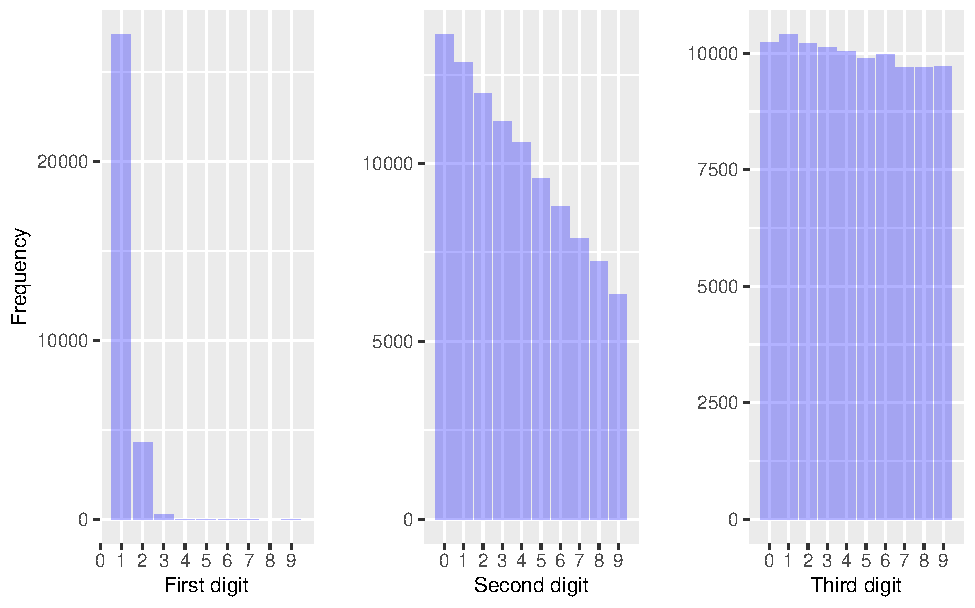
\includegraphics{_main_files/figure-latex/digit-dist-1} 

}

\caption{Frequency distributions of the first-, second-, and third digits. We sampled 100,000 values from a standard normal distribution to create these digit distributions.}\label{fig:digit-dist}
\end{figure}

\subsubsection{Multivariate
associations}\label{multivariate-associations}

Variables or measurements included in one study can have multivariate
associations that might be non-obvious to researchers. Hence, such
relations between variables or measurements might be overlooked by
people who fabricate data. Fabricators might also simply be practically
unable to fabricate data that reflect these multivariate associations,
even if they are aware of these associations. For example, in response
time latencies, there typically is a positive relation between mean
response time and the variance of the response time. Given that the
genuine multivariate relations between different variables arise from
stochastic processes and are not readily known in either their form or
size, these might be difficult to take into account for someone who
wants to fabricate data. As such, using multivariate associations to
discern fabricated data from genuine data might prove worthwhile.

The multivariate associations between different variables can be
estimated from control data that are (arguably) genuine. For example, if
the multivariate association between means (\(M\)s) and standard
deviations (\(SD\)s) is of interest, control data for that same measure
can be collected from the literature. With these control data, a
meta-analysis provides an overall estimate of the multivariate relation
that can subsequently be used to verify the credibility of a set of
statistics.

Specifically, the multivariate associations from the genuine data are
subsequently used to estimate the extremity of an observed multivariate
relation in investigated data. Consider the following fictitious
example, regarding the multivariate association between \(M\)s and
\(SD\)s for a response latency task mentioned earlier. Figure
\ref{fig:multivariate-association} depicts a (simulated) population
distribution of the association (e.g., a correlation) between \(M\)s and
\(SD\)s from the literature (\(N\sim(.123, .1)\)). Assume we have two
papers, each coming from a pool of direct replications providing an
equal number of \(M\)s and corresponding \(SD\)s. Associations between
these statistics are \(0.5\) for Paper 1 and \(0.2\) for Paper 2. From
Figure \ref{fig:multivariate-association} we see that the association in
Paper 1 has a much higher percentile score in the distribution (i.e.,
\(99.995\)th percentile) than that of Paper 2 (i.e., \(78.447\)th
percentile).

\begin{figure}

{\centering 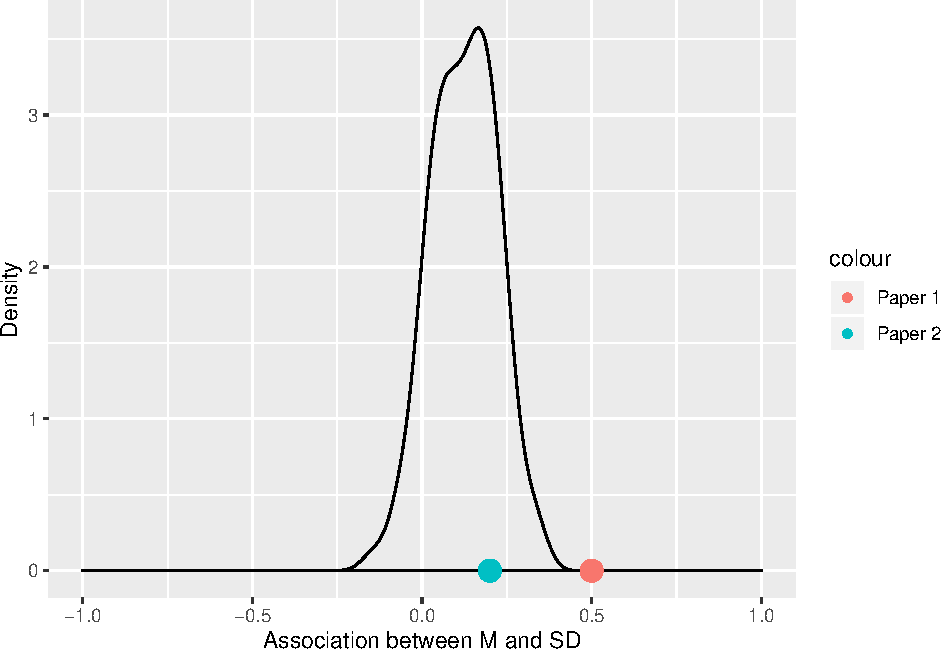
\includegraphics[width=1\linewidth]{_main_files/figure-latex/multivariate-association-1} 

}

\caption{Distribution of 100 simulated observed associations between Ms and SDs for a response latency task; simulated under $N(.123,.1)$. The red- and blue dots indicate observed multivariate associations from fictitious papers. Paper 1 may be considered relatively extreme and of interest for further inspection; Paper 2 may be considered relatively normal.}\label{fig:multivariate-association}
\end{figure}

\section{Study 1 - detecting fabricated summary
statistics}\label{study-1---detecting-fabricated-summary-statistics}

We tested the performance of statistical methods to detect data
fabrication in summary statistics with genuine and fabricated summary
statistics with psychological data. We asked participants to fabricate
data that were supposedly drawn from a study on the anchoring effect
(Tversky and Kahneman
\protect\hyperlink{ref-doi:10.1126ux2fscience.185.4157.1124}{1974};
Jacowitz and Kahneman
\protect\hyperlink{ref-doi:10.1037ux2fe722982011-058}{1995}). The
anchoring effect is a well-known psychological heuristic that uses the
information in the question as the starting point for the answer, which
is then adjusted to yield a final estimate of a quantity. For example:

\begin{quote}
Do you think the percentage of African countries in the UN is above or
below {[}10\% or 65\%{]}? What do you think is the percentage of African
countries in the UN?
\end{quote}

In their classic study, Tversky and Kahneman
(\protect\hyperlink{ref-doi:10.1126ux2fscience.185.4157.1124}{1974})
varied the anchor in this question between 10\% and 65\% and found that
they yielded mean responses of 25\% and 45\%, respectively (Tversky and
Kahneman
\protect\hyperlink{ref-doi:10.1126ux2fscience.185.4157.1124}{1974}). We
chose the anchoring effect because it is well known and because a
considerable amount of (arguably) genuine data sets on the anchoring
heuristic are freely available (\url{https://osf.io/pqf9r}; R. A. Klein
et al.
\protect\hyperlink{ref-doi:10.1027ux2f1864-9335ux2fa000178}{2014}). This
allowed us to compare data knowingly and openly fabricated by our
participants (researchers in psychology) to actual data that can be
assumed to be genuine because they were draw from a large-scale
international project involving many contributing labs (a so-called Many
Labs study). Our data fabrication study was approved by Tilburg
University's Ethics Review Board (EC-2015.50;
\url{https://osf.io/7tg8g/}).

\subsection{Methods}\label{methods-2}

We collected genuine summary statistics from the Many Labs study and
fabricated summary statistics from our participating fabricators for
four anchoring studies: (i) distance from San Francisco to New York,
(ii) human population of Chicago, (iii) height of the Mount Everest, and
(iv) the number of babies born per day in the United States (Jacowitz
and Kahneman
\protect\hyperlink{ref-doi:10.1037ux2fe722982011-058}{1995}). Each of
the four (genuine or fabricated) studies provided us with summary
statistics in a 2 (low/high anchoring) \(\times\) 2 (male/female)
factorial design. Our analysis of the data fabrication detection methods
used the summary statistics (i.e., means, standard deviations, and test
results) of the four anchoring studies fabricated by each participant or
the four anchoring studies that had actually been conducted by each
participating lab in the Many Labs project (R. A. Klein et al.
\protect\hyperlink{ref-doi:10.1027ux2f1864-9335ux2fa000178}{2014}). The
test results available are the main effect of the anchoring condition,
the main effect of gender, and the interaction effect between the
anchoring conditions and gender conditions. For current purposes, a
participant is defined as researcher/lab where the four anchoring
studies' summary statistics originate from. All materials, data, and
analyses scripts are freely available on the OSF
(\url{https://osf.io/b24pq}) and a preregistration is available at
\url{https://osf.io/tshx8/}. Throughout this report, we will indicate
which facets were not preregistered or deviate from the preregistration
(for example by denoting \enquote{(not preregistered)} or
\enquote{(deviation from preregistration)}) and explain the reason of
the deviation.

\subsubsection{Data collection}\label{data-collection}

We downloaded thirty-six genuine data sets from the publicly available
Many Labs (ML) project (\url{https://osf.io/pqf9r}; R. A. Klein et al.
\protect\hyperlink{ref-doi:10.1027ux2f1864-9335ux2fa000178}{2014}). The
ML project replicated several effects across thirty-six locations,
including the anchoring effect in the four studies mentioned previously.
Considering the size of the ML project, the transparency of research
results, and minimal individual gain for fabricating data, we felt
confident to assume these data are genuine. For each of the thirty-six
labs we computed three summary statistics (i.e., sample sizes, means,
and standard deviations) for each of the four conditions in the four
anchoring studies (i.e., \(3\times4\times4\); data:
\url{https://osf.io/5xgcp/}). We computed these summary statistics from
the raw ML data, which were cleaned using the original analysis scripts
from the ML project.

The sampling frame for the participants asked to fabricate data
consisted of 2,038 psychology researchers who published a peer-reviewed
paper in 2015, as indexed in Web of Science (WoS) with the filter set to
the U.S. We sampled psychology researchers to improve familiarity with
the anchoring effect (Tversky and Kahneman
\protect\hyperlink{ref-doi:10.1126ux2fscience.185.4157.1124}{1974};
Jacowitz and Kahneman
\protect\hyperlink{ref-doi:10.1037ux2fe722982011-058}{1995}). We
filtered for U.S. researchers to ensure familiarity with the imperial
measurement system, which is the scale of some of the anchoring studies
and in order to reduce heterogeneity across fabricators.\footnote{We
  discovered that we included several non-U.S. researchers against our
  initial aim. We filtered Web of Science on U.S. origin, but found out
  that this meant that one of the authors on the paper was U.S. based.
  As such, corresponding authors might still be non-U.S. Based on a
  search through the open ended comments of the participant's responses,
  there was no mention of issues in fabricating the data related to the
  metric or imperial system.} We searched WoS on October 13, 2015. In
total, 2,038 unique corresponding e-mails were extracted from 2,014
papers (due to multiple corresponding authors).

From these 2,038 psychology researchers, we e-mailed a random sample of
1,000 researchers to participate in our study (April 25, 2016;
\href{https://osf.io/s4w8r}{osf.io/s4w8r}). We used Qualtrics and
removed identifying information not essential to the study (e.g., no
IP-addresses saved). We informed the participating researchers that the
study would require them to fabricate data and explicitly mentioned that
we would investigate these data with statistical methods to detect data
fabrication. We also clarified to the participants that they could stop
at any time without providing a reason. If they wanted, participants
received a \$30 Amazon gift card as compensation for their participation
if they were willing to enter their email address. They could win an
additional \$50 Amazon gift card if they were one of three top
fabricators (participants were not informed about how we planned to
detect data fabrication; the procedure for this is explained in the Data
Analysis section). We did not inform participants about how we planned
to detect data fabrication. The provided e-mail addresses were unlinked
from individual responses upon sending the bonus gift cards. The full
Qualtrics survey is available at
\href{https://osf.io/rg3qc}{osf.io/rg3qc}.

Each participant was instructed to fabricate 32 summary statistics (4
studies \(\times\) 2 anchoring conditions \(\times\) 2 sexes \(\times\)
2 statistics {[}mean and SD{]}) that corresponded to three hypotheses.
We instructed participants to fabricate results for the following
hypotheses: there is (i) a positive main effect of the anchoring
condition, (ii) no effect of sex, and (iii) no interaction effect
between condition and sex. We fixed the sample sizes in the fabricated
anchoring studies to 25 per cell so that participants did not need to
fabricate sample sizes. These fabricated summary statistics and their
accompanying test results for these three hypotheses serve as the data
to examine the properties of statistical tools to detect data
fabrication.

We provided participants with a template spreadsheet to fill out the
fabricated data, in order to standardize the fabrication process without
restraining the participant in how they chose to fabricate data. Figure
\ref{fig:spreadsheet-study1} depicts an example of this spreadsheet
(original: \url{https://osf.io/w6v4u}). We requested participants to
fill out the yellow cells with fabricated data, which included means and
standard deviations for the four conditions. Using these values, the
spreadsheet automatically computed statistical tests and immediately
showed them in the \enquote{Current result} column instantaneously. If
these results supported the (fabrication) hypotheses, a checkmark
appeared as depicted in Figure \ref{fig:spreadsheet-study1}. We required
participants to copy-paste the yellow cells into Qualtrics. This
provided a standardized response format that could be automatically
processed in the analyses. Technically, participants could provide a
response that did not correspond to the instructions but none of them
did.

\begin{figure}

{\centering 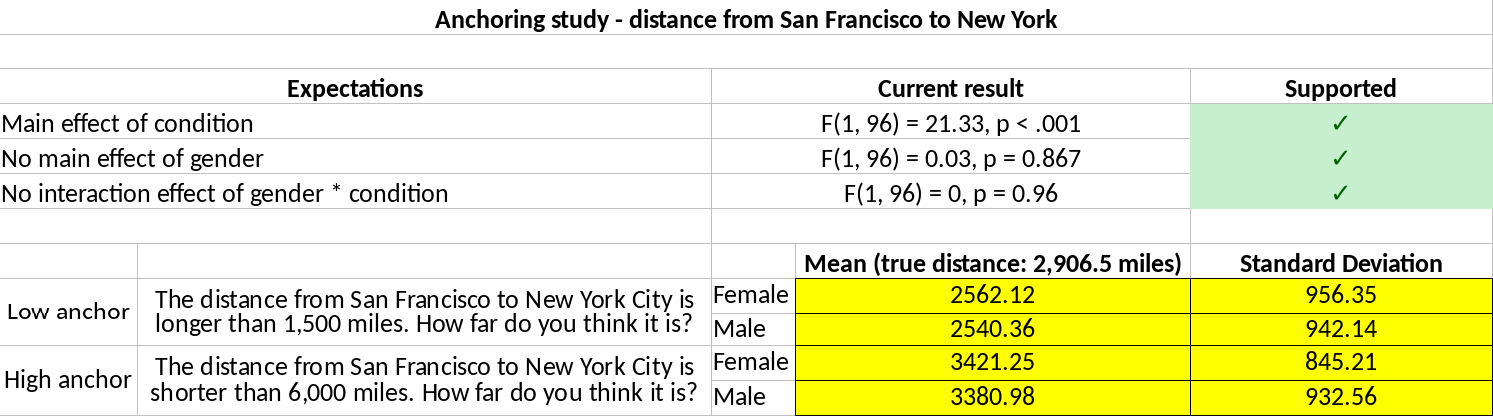
\includegraphics[width=1\linewidth]{./assets/figures/spreadsheet} 

}

\caption{Example of a filled out template spreadsheet used in the fabrication process of Study 1. Respondents fabricated data in the yellow cells, which were used to automatically compute the results of the hypothesis tests, shown in the column "Current result". If the fabricated data confirm the hypotheses, a checkmark appeared in a green cell (one of four template spreadsheets available at https://osf.io/w6v4u).}\label{fig:spreadsheet-study1}
\end{figure}

Upon completion of the data fabrication, we debriefed respondents within
Qualtrics (full survey: \href{https://osf.io/rg3qc/}{osf.io/rg3qc/}).
Respondents self-rated their statistical knowledge (1 = extremely poor,
10 = excellent), what statistical analysis programs they used frequently
(i.e., at least once per week), whether they had ever conducted an
anchoring study themselves, whether they used a random number generator
to fabricate data in this study, whether they fabricated raw data to get
summary statistics, how many combinations of means and standard
deviations they created for each study (on average), and a free-text
description of their fabrication procedures per study. Lastly we
reminded participants that data fabrication is widely condemned by
professional organizations, institutions, and funding agencies alike.
This reminder was intended to minimize potential carry-over effects of
the unethical behavior into actual research practice (Mazar, Amir, and
Ariely \protect\hyperlink{ref-doi:10.1509ux2fjmkr.45.6.633}{2008}).
Using quotum sampling, we collected as many responses as possible for
the available 36 rewards, resulting in 39 fabricated data sets
(\url{https://osf.io/e6zys}; 3 participants did not participate for a
bonus).

\subsubsection{Data analysis}\label{data-analysis}

We analyzed the genuine and fabricated data sets (36 and 39,
respectively), with each data set consisting of summary statistics of
four anchoring studies. The data set is the unit of analysis. Four types
of analyses are conducted on each of the 75 data sets; (i) the reversed
Fisher method, (ii) variance analyses, (iii) the Fisher method applied
to the results of the former two, and (iv) analysis of the effect sizes
of the statistically significant anchoring effect of the four anchoring
studies. Per type of analysis, we examine if we can distinguish the 36
genuine from the 39 fabricated data sets, mainly using Area Under
Receiving Operator Characteristic (AUROC) curves. Below we first
describe each of the four types of analyses, followed by a description
of the AUROC curve analysis.

We conducted two analyses to detect data fabrication using the reversed
Fisher method. More specifically, we conducted one reversed Fisher
method analysis for the four statistically nonsignificant results of the
gender effect (one per anchoring study) and one for the four
statistically nonsignificant interaction effects (one per anchoring
study). This results in two reversed Fisher method results (based on
\(k\)=4) per data set.

For the variance analyses, we substantially deviated from the
preregistration (\url{https://osf.io/tshx8/}) and added multiple
analyses. We analyzed the 16 sample variances (four anchoring studies
\(\times\) four conditions per anchoring study) per lab or participant
in fourteen different ways. Each of the fourteen variance analyses was
conducted using two dispersion of variance measures. One measure
inspects the standard deviation of the sample variances (i.e.,
\(SD_z\)); one measure inspects the range of the sample variances (i.e.,
\(max_z-min_z\)); we ran all 28 analyses with 100,000 iterations from
which we computed the bootstrapped \(p\)-value (see also the Theoretical
Framework). Of these 28 variance analyses (14 for each dispersion of
variances measure), only one was preregistered. This was the variance
analysis combining all 16 sample variances of the four anchoring
studies. Upon analyzing the results of this preregistered variance
analysis, however, we realized that the variance analyses assume that
the included variances are from the same population distribution.
Assuming homogeneous populations of variances is unrealistic for the
four very different anchoring conditions or studies (i.e., they have
outcome measures on very different scales, such as distances in miles
and babies born). Hence, we included variance analyses based on
subgroups, where we analyzed each anchoring study separately (four
variance analyses) or analyzed each anchoring condition of each study
separately (i.e., the low/high anchoring condition collapsed across
gender; eight variance analyses). We also conducted one variance
analysis that combined all variances across studies but takes into
account the subgroups per anchoring condition per study.

We also combined the reversed Fisher method results with the results
from the variance analyses using the original Fisher method. More
specifically, we combined the results from the two reversed Fisher
method analyses (one analysis for the four gender effects and one
analysis for the four interaction effects) with the preregistered
variance analysis (the result of this analysis was used to determine the
three most difficult to detect fabricated datasets and subsequently to
reward the \enquote{best fabricators}). We additionally applied the
Fisher method to results of the reversed Fisher method (two results)
with three different combinations of results of the variance analyses;
based on variance analyses per anchoring study (four results), per
anchoring study \(\times\) condition combination (eight results), and
across all studies and conditions but taking into account heterogeneous
variances per anchoring condition for each study (one result). Hence,
the additional Fisher method analyses were based on six, ten, and three
results, respectively. Throughout these combinations, we only use the
\(SD_z\) dispersion of variance measure for parsimony. Note that the
performance of the Fisher method combining results of various analyses
(the reversed Fisher method and the variance analyses) as we do here is
naturally dependent on the performance of the individual results
included in the combination; if all included results perform well the
Fisher method is bound to perform well and vice versa.

Finally, we looked at statistically significant effect sizes. We
expected fabricated statistically significant effects to be larger than
genuine statistically significant effects. As such, we compared the 75
statistically significant anchoring effects for each of the four
anchoring studies separately (not preregistered).

For each of the previously described statistical methods to detect data
fabrication, we carried out AUROC curve analyses. AUROC analyses
summarize the sensitivity (i.e., True Positive Rate {[}TPR{]}) and
specificity (i.e., True Negative Rate {[}TNR{]}) for various decision
criteria (e.g., \(\alpha=0, .01, .02, ..., .99, 1\)). For our purposes,
AUROC values indicate the probability that a randomly drawn fabricated
and genuine dataset can be correctly classified as fabricated or genuine
based on the result of the analysis (Hanley and McNeil
\protect\hyperlink{ref-doi:10.1148ux2fradiology.143.1.7063747}{1982}).
In other words, if \(AUROC=.5\), correctly classifying a randomly drawn
dataset as fabricated (or genuine) is equal to 50\% (assuming equal
prevalences). For this setting, we follow the guidelines of Youngstrom
(\protect\hyperlink{ref-doi:10.1093ux2fjpepsyux2fjst062}{2013}) and
regard any AUROC value \(<.7\) as poor for detecting data fabrication,
\(.7\leq\) AUROC \(<.8\) as fair, \(.8\leq\) AUROC \(<.9\) as good, and
AUROC \(\geq.9\) as excellent. We conducted all analyses using the
\texttt{pROC} package (Robin et al.
\protect\hyperlink{ref-doi:10.1186ux2f1471-2105-12-77}{2011}).

\subsection{Results}\label{results-3}

Figure \ref{fig:ddfab-density1} shows a group-level comparison of the
genuine- (\(k=36\)) and fabricated (\(k=39\)) datasets, which contain
four \(p\)-values and relevant effect sizes (\(r\)) for each type of
effect (gender, anchoring, interaction) per dataset (i.e., \(75\times4\)
data points for each plot). These group-level comparisons provide a
general overview of the differences between the genuine and fabricated
data. Figure \ref{fig:ddfab-density1} (right and left column) already
indicates that there are few systematic differences between fabricated
and genuine summary statistics from the anchoring studies when
statistically nonsignificant effects are inspected (i.e., gender and
interaction hypotheses). However, there seem to be larger differences
when we required participants to fabricate statistically significant
summary statistics (i.e., anchoring hypothesis; middle column). We
discuss results bearing on the specific tests for data fabrication next.

\begin{figure}
\centering
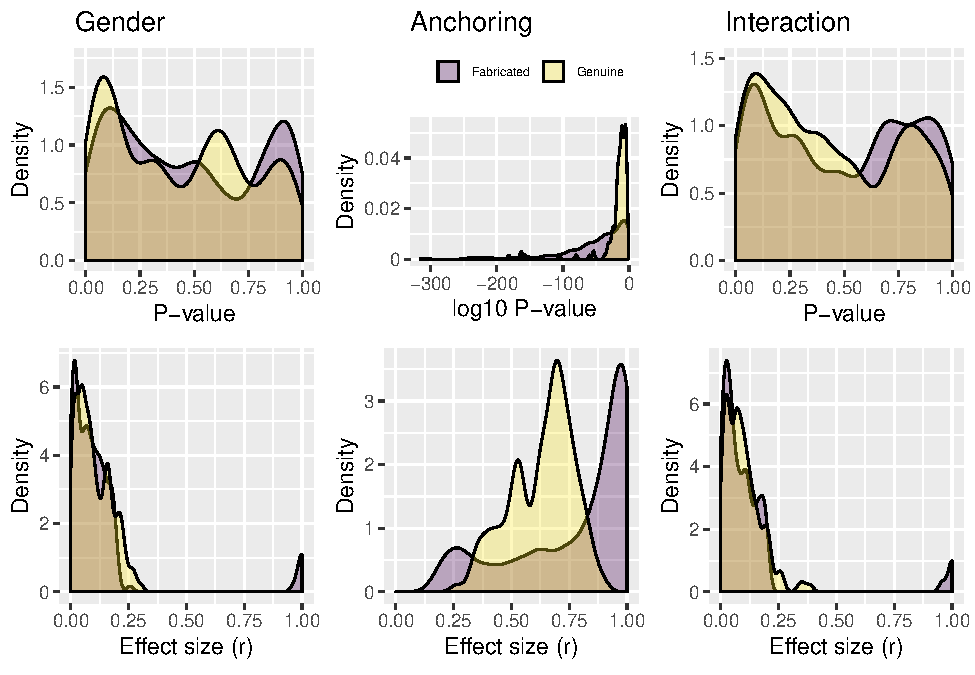
\includegraphics{_main_files/figure-latex/ddfab-density1-1.pdf}
\caption{\label{fig:ddfab-density1}Density distributions of genuine and
fabricated summary statistics across four anchoring studies, per effect
(gender, anchoring, or interaction across columns) and type of result
(p-value or effect size across rows).}
\end{figure}

\subsubsection{\texorpdfstring{\(P\)-value
analysis}{P-value analysis}}\label{p-value-analysis-1}

When we applied the reversed Fisher method to the statistically
nonsignificant effects, results indicated its performance is
approximately equal to chance classification. We found \(AUROC=0.501\),
95\% CI {[}\(0.468\)-\(0.535\){]} for statistically nonsignificant
gender effects and \(AUROC=0.516\), 95\% CI {[}\(0.483\)-\(0.549\){]}
for statistically nonsignificant interaction effects. For the gender
effects, we classified 12 of the 39 fabricated summary statistics as
fabricated (\(\alpha=.01\)) and 6 of the 36 genuine summary statistics
as fabricated (results per respondent available at
\href{https://osf.io/a6jb4}{osf.io/a6jb4}). For the interaction effects,
we classified 11 of the 39 fabricated summary statistics
(\(\alpha=.01\)) and 8 of the 36 genuine summary statistics as
fabricated (results per respondent available at
\href{https://osf.io/jz57p}{osf.io/jz57p}). In other words, results from
this sample indicated that detection of fabricated data using the
distribution of statistically nonsignificant \(p\)-values to detect
excessive amounts of high \(p\)-values does not seem promising.

\subsubsection{Variance analysis}\label{variance-analysis-1}

We expected the dispersion of variances to be lower in fabricated data
as opposed to genuine data. We computed the AUROC values for the
variance analyses with the directional hypothesis that genuine data
shows more variation than fabricated data, using either the dispersion
of variance as captured by the standard deviation of the variances
(i.e., \(SD_z\)) or the range of the variances (i.e., \(max_z-min_z\)).
AUROC results of all 14 analyses (as described in the Data analysis
section) are presented in Table \ref{tab:auc-var1}, one result for each
dispersion of variance measure. Of these 14 results, we only
preregistered the variance analysis inspecting the standardized
variances across all studies under both the \(SD_z\) and \(max_z-min_z\)
operationalizations, assuming unrealistically homogeneous population
variances (\url{https://osf.io/tshx8/}; second row of Table
\ref{tab:auc-var1}). As we did not preregister the other variance
analyses, these should be considered exploratory.

\begin{table}[!h]

\caption{\label{tab:auc-var1}Area Under Receiving Operator Characteristic (AUROC) values of each variance analysis and operationalization, including its 95 percent Confidence Interval. 'Heterogeneity' assumes unequal population variances for the low- and high anchoring conditions, whereas 'homogeneity' assumes equal population variances across anchoring conditions in the same study. We preregistered only the analyses in the second row.}
\centering
\resizebox{\linewidth}{!}{
\begin{tabular}{llll}
\toprule
Population variance assumption & Study & $SD_z$ & $max_{z}-min_{z}$\\
\midrule
\rowcolor{gray!6}  Heterogeneity & Overall & 0.761 [0.733-0.788] & 0.827 [0.8-0.853]\\
Homogeneity & Overall & 0.264 [0.235-0.293] & 0.544 [0.507-0.58]\\
\rowcolor{gray!6}  Homogeneity & Study 1 & 0.373 [0.339-0.406] & 0.488 [0.474-0.502]\\
Homogeneity & Study 2 & 0.395 [0.36-0.429] & 0.634 [0.608-0.66]\\
\rowcolor{gray!6}  Homogeneity & Study 3 & 0.498 [0.463-0.533] & 0.563 [0.539-0.588]\\
\addlinespace
Homogeneity & Study 4 & 0.401 [0.367-0.435] & 0.561 [0.527-0.594]\\
\rowcolor{gray!6}  Heterogeneity & Study 1, low anchoring & 0.438 [0.406-0.47] & 0.487 [0.481-0.493]\\
Heterogeneity & Study 1, high anchoring & 0.615 [0.582-0.647] & 0.501 [0.492-0.51]\\
\rowcolor{gray!6}  Heterogeneity & Study 2, low anchoring & 0.652 [0.621-0.683] & 0.625 [0.607-0.643]\\
Heterogeneity & Study 2, high anchoring & 0.556 [0.523-0.589] & 0.528 [0.515-0.541]\\
\addlinespace
\rowcolor{gray!6}  Heterogeneity & Study 3, low anchoring & 0.643 [0.612-0.674] & 0.542 [0.53-0.553]\\
Heterogeneity & Study 3, high anchoring & 0.747 [0.719-0.775] & 0.691 [0.669-0.712]\\
\rowcolor{gray!6}  Heterogeneity & Study 4, low anchoring & 0.667 [0.636-0.697] & 0.595 [0.577-0.614]\\
Heterogeneity & Study 4, high anchoring & 0.798 [0.773-0.823] & 0.756 [0.733-0.779]\\
\bottomrule
\end{tabular}}
\end{table}

Under the (in hindsight unrealistic) assumption of homogeneous
population variances, our preregistered variance analyses did not
perform above chance level. Using the standard deviation of the
variances (i.e., \(SD_z\)) as dispersion of variance measure, the
results are: \(AUROC=0.264\), 95\% CI {[}\(0.235\)-\(0.293\){]}. With
this statistic, we classified 0 of the 39 fabricated summary statistics
(\(\alpha=.01\)) and 0 of the 36 genuine summary statistics as
fabricated (results per respondent available at
\href{https://osf.io/9cjdh}{osf.io/9cjdh}). Using the range of the
variances (i.e., \(max_z-min_z\)) as dispersion of variance, the results
are: \(AUROC=0.544\), 95\% CI {[}\(0.507\)-\(0.58\){]}.\\
With this statistic, we detected 39 of the 39 fabricated summary
statistics as fabricated (\(\alpha=.01\)) and 36 of the 36 genuine
summary statistics as fabricated (results per respondent available at
\href{https://osf.io/2ts6b}{osf.io/2ts6b}). Comparing the results
between \(SD_z\) and \(max_z-min_z\) indicates that the range of the
variances measure seems more robust to the violations of the assumption
of homogeneous variances than the standard deviation of the variances
measure. Overall these results indicate that a violation of the
homogeneity assumption may undermine analyses on heterogeneous
variances. These assumptions should be made more explicit and checked
whenever possible, to prevent improper use.

We conducted exploratory analyses that take into account the
heterogeneity of variances across conditions and studies, which
sometimes also resulted in improved performance to detect data
fabrication. Analyses separated per study or anchoring condition show
variable \(AUROC\) results (ranging from 0.373-0.798; rows 3-14 in Table
\ref{tab:auc-var1}). Using the standard deviation of variances (i.e.,
\(SD_z\); row 1 in Table \ref{tab:auc-var1}) in a heterogeneous manner
across the conditions and studies, \(AUROC=0.761\), 95\% CI
{[}\(0.733\)-\(0.788\){]}. With this statistic, we classified 9 of the
39 fabricated summary statistics as fabricated (\(\alpha=.01\)) and 0 of
the 36 genuine summary statistics (results per respondent available at
\href{https://osf.io/srpg9}{osf.io/srpg9}). Using the range of variances
(i.e., \(max_z-min_z\)) in a heterogeneous manner across the conditions
and studies, \(AUROC=0.827\), 95\% CI {[}\(0.8\)-\(0.853\){]}. With this
statistic, we classified the same 9 of the 39 fabricated summary
statistics as fabricated (\(\alpha=.01\)) and 0 of the 36 genuine
summary statistics (results per respondent available at
\href{https://osf.io/93rek}{osf.io/93rek}).

\subsubsection{\texorpdfstring{Combining \(p\)-value and variance
analyses}{Combining p-value and variance analyses}}\label{combining-p-value-and-variance-analyses}

Our preregistered analysis combined the homogeneous variance analysis
across studies and conditions with the \(p\)-value analyses of the
gender and interaction effects. This combined analysis yielded
\(AUROC=0.58\), 95\% CI {[}0.548-0.611{]}. With this statistic, we
classified 19 of the 39 fabricated summary statistics as fabricated
(\(\alpha=.01\)) and 16 of the 36 genuine summary statistics (results
per respondent available at \href{https://osf.io/hq29t}{osf.io/hq29t}).
Given that the combination method would be expected to perform not much
better than its constituent results it logically follows that the
combination of \(p\)-values and variance analyses performs this poorly.

The poor performance is in part is due to the unrealistic assumption of
homogeneous variances in the variance analysis; we explored the efficacy
of other combinations that loosen this assumption. First, we split the
variance analyses per study and included four variance analysis results
instead of one when we analyzed them overall; \(AUROC=0.605\), 95\% CI
{[}0.573-0.636{]}. With this statistic, we classified 20 of the 39
fabricated summary statistics as fabricated (\(\alpha=.01\)) and 13 of
the 36 genuine summary statistics (results per respondent available at
\href{https://osf.io/r8pf5}{osf.io/r8pf5}). Second, we split the
variance analyses further, splitting across conditions within studies.
This adds another four variance analyses (a total of eight);
\(AUROC=0.684\), 95\% CI {[}0.655-0.714{]}. With this statistic, we
classified 25 of the 39 fabricated summary statistics as fabricated
(\(\alpha=.01\)) and 15 of the 36 genuine summary statistics (results
per respondent available at \href{https://osf.io/sv35k}{osf.io/sv35k}).
Finally, we replaced the original homogeneous variance analysis (row 2
in Table \ref{tab:auc-var1}) with the overall and heterogeneous variance
analysis (row 1 in Table \ref{tab:auc-var1}); \(AUROC=0.647\), 95\% CI
{[}0.616-0.677{]}. With this statistic, we classified 23 of the 39
fabricated summary statistics as fabricated (\(\alpha=.01\)) and 16 of
the 36 genuine summary statistics (results per respondent available at
\href{https://osf.io/zt3nk}{osf.io/zt3nk}). As the \(AUROC\)s of the
combination method did not exceed that of the variance analyses alone,
we conclude that the combination method failed to outperform the
variance analyses.

\subsubsection{Extreme effect sizes}\label{extreme-effect-sizes-1}

Using the statistically significant effect sizes from the anchoring
studies, we differentiated between the fabricated and genuine results
fairly well. Figure \ref{fig:ddfab-density1} (middle column, second row)
indicates that the fabricated statistically significant effects were
considerably different from the genuine ones. When we inspected the
effect size distributions (\(r\)), we saw that the median fabricated
effect size across the four studies was \(0.891\) whereas the median
genuine effect size was considerably smaller (\(0.661\); median
difference across the four anchoring effects \(0.23\)). In contrast to
the fabricated nonsignificant effects, which resembled the genuine data
quite well, the statistically significant effects seem to have been
harder to fabricate for the participants. More specifically, the
\(AUROC\) for the studies approximate .75 each (\(0.743\), 95\% CI
{[}\(0.712\)-\(0.774\){]}; \(0.734\), 95\% CI {[}\(0.702\)-\(0.767\){]};
\(0.737\), 95\% CI {[}\(0.706\)-\(0.768\){]}; \(0.755\), 95\% CI
{[}\(0.724\)-\(0.786\){]}; respectively). Figure \ref{fig:ddfab-es1}
depicts the density distributions of the genuine and fabricated effect
sizes per anchoring study, which shows the extent to which the density
of the fabricated effect sizes exceeds the maximum of the genuine effect
sizes. For instance, the percentage of fabricated statistically
significant anchoring effect sizes that is larger than all 36 genuine
statistically significant anchoring effect sizes is 59\% in Study 1,
64.1\% in Study 2, 53.8\% in Study 3, and 66.7\% in Study 4. Based on
these results, it seems that using extreme effect sizes to detect
potential data fabrication may be is a parsimonious and fairly effective
method.

\begin{figure}

{\centering 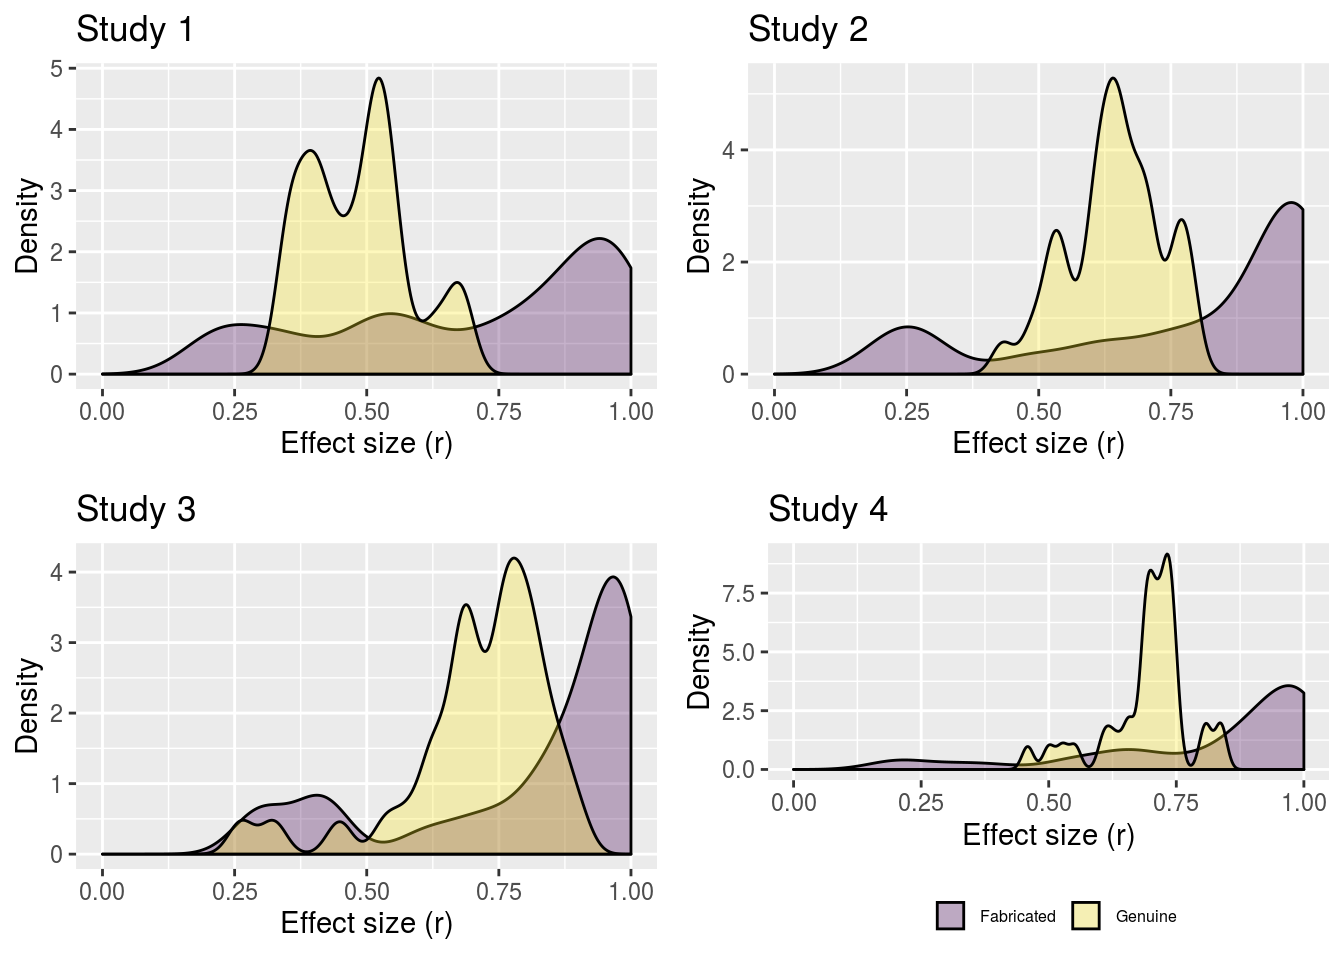
\includegraphics[width=1\linewidth]{_main_files/figure-latex/ddfab-es1-1} 

}

\caption{Density distributions of genuine and fabricated anchoring effect sizes for each of the four anchoring studies.}\label{fig:ddfab-es1}
\end{figure}

\subsubsection{Fabricating effects with Random Number Generators
(RNGs)}\label{fabricating-effects-with-random-number-generators-rngs}

Fabricated effects might seem more genuine when participants used Random
Number Generators (RNGs). RNGs are typically used in computer-based
simulation procedures where data are generated that are supposed to
arise from probabilistic processes. Given that our framework of
detecting data fabrication rests on the lack of intuitive understanding
of humans at drawing values from probability distributions, those
participants who used an RNG might come closer to fabricating seemingly
genuine data, leading to more difficult to detect fabricated data. The
analyses presented next were not preregistered.

We split our analyses for those 11 participants who indicated using RNGs
and the remaining 28 participants who indicated not to have used RNGs.
Figure \ref{fig:rng-density1} shows the same density distributions as in
Figure \ref{fig:ddfab-density1}, except that this time the density
distributions of the fabricated data are split between these two groups.

\begin{figure}
\centering
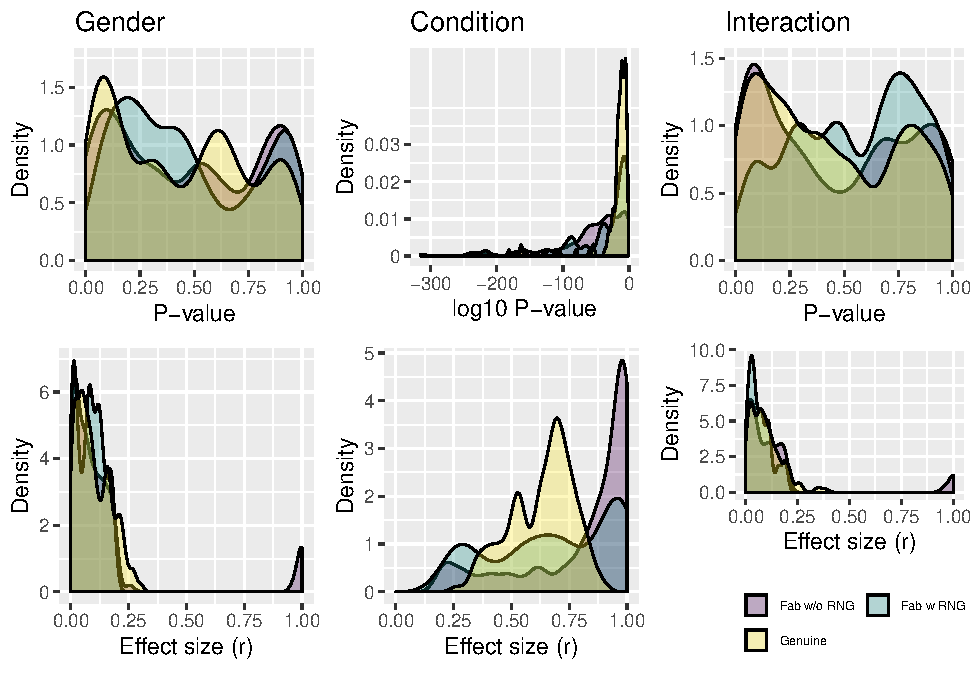
\includegraphics{_main_files/figure-latex/rng-density1-1.pdf}
\caption{\label{fig:rng-density1}Density distributions of p-values and
effect sizes for the gender effect, the anchoring effect, and the
interaction effect across the four anchoring studies. This figure is
similar to Figure \ref{fig:ddfab-density1}, except that each panel now
separates the density distributions for fabricated results using a
random number generator (RNG), fabricated results without using a RNG,
and genuine effects. Respondents self-selected to use (or not use) RNGs
in their fabrication process.}
\end{figure}

Figure \ref{fig:rng-density1} suggests that using RNGs may have resulted
in less exaggerated anchoring effect sizes, but still larger than
genuine ones. Furthermore, it seems that the use of RNGs produced
somewhat more uniformly distributed statistically nonsignficant
\(p\)-values than those without RNGs. For effect sizes, Table
\ref{tab:rng-auc1} specifies the differences in sample estimates of the
\(AUROC\) between the groups of fabricated results with and without RNGs
(as compared to the genuine data). These results indicate that the
fabricated effect sizes from participants who used RNGs are relatively
more difficult to detect compared to data from participants who did not
use a RNG (illustratively, the simple mean of the left column of Table
\ref{tab:rng-auc1} is 0.604 compared to the right column simple mean of
0.797). The numbers presented inTable \ref{tab:rng-auc1} can be
interpreted as the probability that the larger effect is fabricated,
when presented with one genuine and fabricated effect size. For
nonsignificant \(p\)-values, we obtained the following \(AUROC\) values;
gender, with RNG \(AUROC=0.455\) 95\% CI {[}\(0.405\)-\(0.504\){]},
without RNG \(AUROC=0.52\) 95\% CI {[}\(0.482\)-\(0.557\){]};
interaction, with RNG \(AUROC=0.601\) 95\% CI {[}\(0.558\)-\(0.644\){]},
without RNG \(AUROC=0.482\) 95\% CI {[}\(0.444\)-\(0.52\){]}). For the
best performing variance analysis (i.e., heterogeneity over all four
anchoring studies with \(max_z-min_z\)) classification performance does
not seem to be systematically different between those data fabricated
with (\(AUROC=0.78\) 95\% CI {[}\(0.728\)-\(0.833\){]}) or without RNGs
(\(AUROC=0.845\) 95\% CI {[}\(0.817\)-\(0.874\){]}).

\begin{table}[!h]

\caption{\label{tab:rng-auc1}AUROC values for detecting data fabrication based on effect sizes for those participants who used Random Number Generators (RNGs) and those participants who did not use RNGs, including 95 percent confidence interval. Split based on self-report data on whether RNGs were used by the participant.}
\centering
\begin{tabular}{lll}
\toprule
Study & $AUROC$ RNG, $k=11$ & $AUROC$ no RNG, $k=28$\\
\midrule
\rowcolor{gray!6}  Study 1 & 0.553 [0.489-0.617] & 0.817 [0.785-0.85]\\
Study 2 & 0.641 [0.578-0.705] & 0.771 [0.734-0.807]\\
\rowcolor{gray!6}  Study 3 & 0.578 [0.512-0.645] & 0.8 [0.767-0.832]\\
Study 4 & 0.641 [0.581-0.702] & 0.8 [0.764-0.835]\\
\bottomrule
\end{tabular}
\end{table}

Note that participants self-selected the use of RNGs or not, and that we
did not preregister these analyses. Given the small number of results
(11 versus 28), we did not statistically test the differences due to
lack of statistical power, and only present descriptive results.

\subsection{Discussion}\label{discussion-4}

We presented the first controlled study on detecting data fabrication at
the level summary statistics. As far as we could tell, previous efforts
only looked at group-level comparisons of genuine and fabricated data
(Akhtar-Danesh and Dehghan-Kooshkghazi
\protect\hyperlink{ref-doi:10.1186ux2f1471-2288-3-18}{2003}), inspected
properties of individually fabricated sets of data without comparing
them to genuine data, or did not contextualize these data in a realistic
study with specific hypotheses (Mosimann, Wiseman, and Edelman
\protect\hyperlink{ref-doi:10.1080ux2f08989629508573866}{1995}). We
explicitly asked researchers to fabricate results for an effect within
their research domain (i.e., the anchoring effect), which was
contextualized in realistic hypotheses, and compared them to genuine
data on the same effect. We investigated the performance of the reversed
Fisher method, variance analyses, combinations of these two methods, and
statistically significant effect sizes to detect fabricated data.

Methods related to classifying statistically significant summary
statistics (i.e., effect sizes and variance analyses) performed fairly
well, whereas those relating to statistically nonsignificant summary
statistics (i.e., \(p\)-value analyses) performed poorly.
Non-preregistered results suggest that variance analyses performed
similarly or marginally better than using statistically significant
effect sizes in this sample. Hence, we recommend using methods that
investigate statistically significant effects to detect potential data
fabrication, but prior to their application their assumptions should be
well understood and tested.

We noted that the assumption of homogeneous population variances in the
variance analyses has not previously been explicated nor tested for
robustness to violations. In Simonsohn
(\protect\hyperlink{ref-doi:10.1177ux2f0956797613480366}{2013}) it
remains implicit that the variances grouped together in an analysis
should arise from a homogeneous population distribution. Our results
indicated that the classification performance of variance analyses may
strongly depend on satisfying this assumption, that is, the performance
of the method is not robust to violations of the homogeneity assumption.
The alternative approach to variance analyses using the range of
variances instead of their standard deviation (i.e., \(max_{z}-min_{z}\)
rather than \(SD_z\)) seemed to be more robust to violations of the
homogeneity assumption. This comparison was not preregistered and its
performance could be studied further. Nonetheless, based on the success
of using the dispersion of variances, we recommend to use variance
analyses with subgrouping of variances into those that are likely to be
from the same population distribution (e.g., based on anchoring
condition in the datasets studied here) and also consider using the
range of standard deviations \(max_{z}-min_{z}\)).

Of all methods we applied, we obtained the best performance using the
heterogeneous variance analyses, which resulted in detecting 9 out of 39
fabricated data sets (23\%) and no false positives (0; \(\alpha=.01\)).
Performance using (only) the statistically effect sizes was comparably
good. Consequently, we failed to detect the majority of the fabricated
datasets using statistical methods based on nonsignificant \(p\)-values,
consistency of variances, and effect sizes. More worrisome is that for
many methods the false positive rate was high, in one case even 100\%
(using \(max_{z}-min_{z}\) based on the assumption of homogeneity of all
variances).

Our finding that statistical analyses of data with fabrication detection
tools may not be robust to violations of their assumptions has
implications for investigations of research misconduct. Our results
demonstrate that improper model specification can result in classifying
anything as potentially fabricated (i.e., high false positive rate),
which comes at high costs for all parties involved. Moreover, improper
model specification may also result in a high false negative rate, as in
our homogeneous variance analyses, resulting in a much too low \(AUROC\)
values (e.g., \(AUROC=.264\)). Our sometimes high false positive and
false negative rates are especially worrisome in light of widespread
application of statistical methods to screen for potential problematic
studies (e.g., Carlisle
\protect\hyperlink{ref-doi:10.1111ux2fanae.13938}{2017}\protect\hyperlink{ref-doi:10.1111ux2fanae.13938}{a};
Loadsman and McCulloch
\protect\hyperlink{ref-doi:10.1111ux2fanae.13962}{2017}), when their
validation is based on the criterion that the methods proved useful to
detect problematic data in isolated research misconduct cases the past
(e.g., Carlisle
\protect\hyperlink{ref-doi:10.1111ux2fj.1365-2044.2012.07128.x}{2012};
Miller \protect\hyperlink{ref-doi:10.1111ux2fanae.13165}{2015}; Carlisle
and Loadsman \protect\hyperlink{ref-doi:10.1111ux2fanae.13650}{2016}).
For instance, the usefulness of the reversed Fisher method to detect
problematic data in the past (Anonymous
\protect\hyperlink{ref-foerster-complaint}{2012}; Levelt
\protect\hyperlink{ref-Levelt2012}{2012}) should not be taken as
evidence of its validity for general application. Our study highlights
the importance of validating methods with genuine reference data, before
using these tools to flag potential problematic papers. Note that
concerns like this have been expressed before (Kharasch and Houle
\protect\hyperlink{ref-doi:10.1097ux2faln.0000000000001875}{2017}\protect\hyperlink{ref-doi:10.1097ux2faln.0000000000001875}{a};
Mascha, Vetter, and Pittet
\protect\hyperlink{ref-doi:10.1213ux2fane.0000000000002415}{2017};
Piraino \protect\hyperlink{ref-doi:10.1101ux2f179135}{2017}; Kharasch
and Houle
\protect\hyperlink{ref-doi:10.1111ux2fanae.14147}{2017}\protect\hyperlink{ref-doi:10.1111ux2fanae.14147}{b};
Moppett \protect\hyperlink{ref-doi:10.1111ux2fanae.14048}{2017}).

Our results warrant further research on the underlying assumptions and
validity of statistical approaches to detect potential data fabrication
using summary statistics. This further research can help determine or
prevent model misspecification, both in the assumptions of the
statistical models and the psychology theory for specific ways of
fabricating data before standard application of these methods in
practice (see also Carlisle
\protect\hyperlink{ref-doi:10.1111ux2fanae.14148}{2017}\protect\hyperlink{ref-doi:10.1111ux2fanae.14148}{b}).

For the reversed Fisher method that focused on the overly consistent
results for effects that are expected to follow the null hypothesis,
results indicated that participants did not fabricate excessive amounts
of high \(p\)-values (i.e., closer to 1 than expected by chance) when
told to fabricate statistically nonsignificant effects. This ran against
our prediction that the absence of a true effect would prompt
fabricators to fabricate results that do not contain enough randomness,
resulting in too many high \(p\)-values. This is particularly noteworthy
because this tenet has been helpful or even central to several known
cases of research misconduct (Anonymous
\protect\hyperlink{ref-foerster-complaint}{2012}; Levelt
\protect\hyperlink{ref-Levelt2012}{2012}). However, different from these
specific cases, the results we asked participants to fabricate were
first-order results (i.e., those immediately observable to the
participants), whereas in the Stapel and Förster case, the reversed
Fisher method showed potential data fabrication across second order
results (i.e., similarity of means of experiments of different papers in
the case of Stapel, or linearity test of first-order results in case of
Förster). Hence, although our results indicate that the reversed Fisher
method often does not perform well for inspecting first-order results,
it may still perform well in isolated cases, particularly when applied
to higher order results (see also Haldane
\protect\hyperlink{ref-Haldane1948-nm}{1948}).

Results of our reversed Fisher method are inexact because we used
dependent fabricated results, which we did not take into account in our
analyses. More specifically, for the \(p\)-value analyses we analyzed
the four \(p\)-values from (for example) the gender effect across the
four fabricated studies for one participant. This might have violated
the assumption of independence, hence may have resulted in biased
results of this test. Neither our analyses of the effect sizes nor our
variance analyses suffer from this issue.

Analyses combining different data fabrication tools may not perform
better than analyses based on a single tool, which also has implications
for research misconduct investigations. First, a fabricated dataset does
not imply that all tools should hint at data fabrication; fabricated
data may resemble genuine data in some respects but not in others.
Second, focusing on one aspect that best distinguishes fabricated from
genuine data may perform best. The problem is then to identify that
aspect, preferably before conducting the investigation. Our study
suggests to focus on the analysis of properties of statistically
significant effect sizes, whereas some fraud cases suggested to focus on
properties of statistically nonsignificant effect sizes. We recommend,
in cases of multiple independent possibly fabricated studies, to use
several tools to identify possible fabrication in one study, and then
apply and test the tools that worked to the other possibly fabricated
studies (cross-validation). Importantly, we wish to emphasize that it
does not make sense to require that \emph{all} tools signal fabrication;
as fabricated data may resemble genuine data in some respects, absence
of one or several signals should not be considered as evidence of no
fabrication.

We also considered the possibility that the use of a Random Number
Generator (RNG) to fabricate summary statistics could decrease the
probability of detecting a fabricated dataset. Although we did not
preregister these analyses, descriptive results suggest that using RNGs
decreases the performance of using effect sizes to classify fabricated
from genuine data. On the other hand, using RNGs did not substantially
decrease the performance of the variance analysis that analyzed the
effect sizes bearing on anchoring. Note that our results are solely
descriptive due to too small group sizes for meaningful comparisons. We
will investigate in Study 2 whether using RNGs affects the performance
of detecting data fabrication in a similar fashion and revisit this
issue in the general discussion.

We note that our presented results might be particular to the anchoring
effect and not replicable with other effects. First, as opposed to many
other effects in psychology, many data on the anchoring effect are
already available and fabricators may have used these data when
fabricating theirs. Second, fabrication strategies may be dependent on
the type of effect or measurement that is being fabricated. In the
anchoring studies, data needed to be fabricated for numbers that are in
the hundreds or thousands. Such relatively large values might feel more
unintuitive to think about than smaller numbers in the singles or tens
that might appear in other research contexts. Hence, we might be better
at detecting potential data fabrication in data of our study compared to
most other studies because of this increased lack of intuitiveness.
Other kinds of studies that are easier for fabricators to think about in
terms of fabricating realistic data might prove more difficult to
classify. For example, fabrication of data of Likert scales may be more
difficult (or easier) to detect than fabrication of continuous data.

Despite testing various statistical methods to detect data fabrication,
we did not test all available statistical methods to detect data
fabrication in summary statistics. SPRITE (Heathers et al.
\protect\hyperlink{ref-doi:10.7287ux2fpeerj.preprints.26968v1}{2018}),
GRIM (Brown and Heathers
\protect\hyperlink{ref-doi:10.1177ux2f1948550616673876}{2016}), and
GRIMMER (Anaya
\protect\hyperlink{ref-doi:10.7287ux2fpeerj.preprints.2400v1}{2016}) are
some examples of other statistical methods that test for problematic or
fabricated summary statistics (see also Buyse et al.
\protect\hyperlink{ref-buyse1999}{1999}). However, these methods were
not applicable in the studies we presented, because they require ordinal
scale measures. It seems that, combined with the question of whether
current results of detecting fabricated data replicate in Likert scale
studies, validating these other methods would be a fruitful avenue for
further research.

\section{Study 2 - detecting fabricated individual level
data}\label{study-2---detecting-fabricated-individual-level-data}

In Study 2 we tested the performance of statistical methods to detect
fabrication of individual level (or raw) data. Our procedure is
comparable to that used in Study 1: We again asked actual researchers to
fabricate data that they thought would go undetected. However, instead
of summary statistics, in Study 2 we asked participants to fabricate
lower level data (i.e., individual level data) and included a
face-to-face interview in which we debriefed participants on how they
fabricated their data (Hartgerink et al.
\protect\hyperlink{ref-doi:10.5281ux2fzenodo.832490}{2017}). A
preregistration of this study occurred during the seeking of funding
(Hartgerink, Wicherts, and Assen
\protect\hyperlink{ref-doi:10.3897ux2frio.2.e8860}{2016}) and during
data collection (\url{https://osf.io/fc35g}). Just like Study 1, this
study was approved by the Tilburg Ethics Review Board (EC-2015.50;
\url{https://osf.io/7tg8g/}).

To test the validity of statistical methods to detect data fabrication
in individual level data, we investigated individual level data of the
classic Stroop experiment (Stroop
\protect\hyperlink{ref-doi:10.1037ux2fh0054651}{1935}). In a Stroop
experiment, participants were asked to determine the color a word is
presented in (i.e., word colors) and where the word also reads a color
(i.e., color words). The presented word color (i.e., \enquote{red},
\enquote{blue}, or \enquote{green}) can be either presented in the
congruent color (e.g., \enquote{red} presented in red) or an incongruent
color (e.g., \enquote{red} presented in green). The dependent variable
in a Stroop experiment is the response latency, typically in
milliseconds. Participants in actual Stroop studies are usually
presented with a set of these Stroop tasks, where the mean and standard
deviation per condition serve as the individual level data for analyses
(see also Ebersole et al.
\protect\hyperlink{ref-doi:10.1016ux2fj.jesp.2015.10.012}{2016}). The
Stroop effect is often computed as the difference in mean response
latencies between the congruent and incongruent conditions.

\subsection{Methods}\label{methods-3}

\subsubsection{Data collection}\label{data-collection-1}

We collected twenty-one genuine data sets on the Stroop task from the
Many Labs 3 project (\url{https://osf.io/n8xa7/}; Ebersole et al.
\protect\hyperlink{ref-doi:10.1016ux2fj.jesp.2015.10.012}{2016}). Many
Labs 3 (ML3) includes 20 participant pools from universities and one
online sample (the original preregistration mentioned 20 data sets,
accidentally overlooking the online sample; Hartgerink, Wicherts, and
Assen \protect\hyperlink{ref-doi:10.3897ux2frio.2.e8860}{2016}). Similar
to Study 1, we assumed these data to be genuine due to the minimal
individual gains for fabricating data and the transparency of the
project. Using the original raw data and analysis script from ML3
(\url{https://osf.io/qs8tp/}), we computed the mean (\(M\)) and standard
deviation (\(SD\)) of response latencies for each participant in both
within-subjects conditions of congruent trials and incongruent trials
(i.e., two \(M\)-\(SD\) combinations for each participant). This format
was also the basis for the template spreadsheet that we requested
participants to use to supply the fabricated data (see also Figure
\ref{fig:spreadsheet-study2} or \url{https://osf.io/2qrbs/}). We
calculated the Stroop effect as a \(t\)-test of the difference between
the congruent and incongruent conditions
(\(H_0:\mu_{\bar{X}_1-\bar{X}_2}=0\)).

\begin{figure}
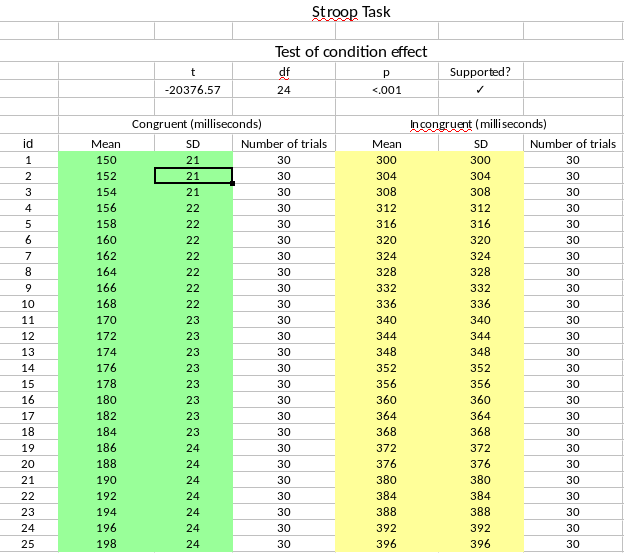
\includegraphics[width=1\linewidth]{./assets/figures/spreadsheet2} \caption{Example of a filled out template spreadsheet used in the fabrication process for Study 2. Respondents fabricated data in the yellow cells and green cells, which were used to compute the results of the hypothesis test of the condition effect. If the fabricated data confirmed the hypotheses, a checkmark appeared (upper right). This template is available at https://osf.io/2qrbs.}\label{fig:spreadsheet-study2}
\end{figure}

We collected 28 fabricated data sets on the Stroop task in a two-stage
sampling procedure. First, we invited 80 Dutch and Flemish psychology
researchers who published a peer-reviewed paper on the Stroop task
between 2005-2015 as available in the Thomson Reuters' Web of Science
database. We selected Dutch and Flemish researchers to allow for
face-to-face interviews on how the data were fabricated. We chose the
period 2005-2015 to prevent a decrease in the probability that the
corresponding author would still be reachable via the given
corresponding e-mail address. The database was searched on October 10,
2016 and 80 unique e-mails were retrieved from 90 publications. Two of
these 80 researchers (2.5\%) we contacted actually ended up
participating in our study. Subsequently, we implemented a second,
unplanned sampling stage where we collected e-mails from all
PhD-candidates, teachers, and professors of psychology-related
departments at Dutch universities. This resulted in 1,659 additional
unique e-mails that we subsequently invited to participate in this
study. Due to a malfunction in Qualtrics' quotum sampling, we
oversampled, resulting in 28 participants instead of the originally
intended 20 participants. The second sampling scheme was not part of the
original ethics application, but was considered crucial to obtain a
sufficiently large sample.

Each participant received instructions on the data fabrication task via
Qualtrics and was allowed to fabricate data until the face-to-face
interview took place. In other words, each participant could take the
time they wanted or needed to fabricate the data as extensively as they
liked. Each participant received downloadable instructions (original:
\url{https://osf.io/7qhy8/}) and the template spreadsheet via Qualtrics
(see Figure \ref{fig:spreadsheet-study2}; \url{https://osf.io/2qrbs/}).
The interview was scheduled via Qualtrics with JGV, who blinded the rest
of the research team from the identifying information of each
participant and the date of the interview. All interviews took place
between January 31 and March 3, 2017. To incentivize researchers to
participate, they received 100 euros for participation; to incentivize
them to fabricate (supposedly) hard to detect data they could win an
additional 100 euros if they belonged to one out of three top
fabricators (see Data Analysis section for exact method used).
Participants were not informed about how we planned to detect data
fabrication; we used the combined Fisher method (described next). JGV
transcribed the contents of the interview and CHJH blind-reviewed these
transcripts to remove any potentially personally identifiable
information (these transcripts are freely available for anyone to use at
\url{https://doi.org/10.5281/zenodo.832490}).

\subsubsection{Data analysis}\label{data-analysis-1}

To detect data fabrication in individual level data using statistical
tools, we performed a total of sixteen analyses per dataset
(preregistration: \url{https://osf.io/ecxvn/}) for each of the 21
genuine datasets and 28 fabricated datasets. These sixteen analyses
consisted of four Newcomb-Benford Law (NBL) digit analyses, four
terminal digit analyses, two variance analyses, four multivariate
association analyses (deviated from preregistration in that we used a
parametric approach instead of the planned non-parametric approach), a
combination test of these methods, and effect sizes at the summary
statistics level (the latter test replicated Study 1 and was not
preregistered). We had one dataset for each participant fabricating data
and for each lab in the Many Labs study, amounting to 49 datasets.

For the digit analyses (NBL and terminal), we separated the 25 \(M\)s
and 25 \(SD\)s per within-subjects condition and conducted
\(\chi^2\)-tests for each per data set. As such, for one data set, we
conducted digit analyses on the digits of (i) the mean response
latencies in the congruent condition, (ii) the mean response latencies
in the incongruent condition, (iii) the standard deviation of the
response latencies in the congruent condition, and (iv) the standard
deviation of the response latencies in the incongruent condition. For
the NBL, we used the first (or leading) digit, whereas for the terminal
digit analyses we tested the same sets but on the final digit.

For the variance analyses, we analyzed the 25 standard deviations of the
response latencies in the congruent condition for excessive consistency
separately from the 25 standard deviations of the incongruent condition.
We conducted this analysis for each genuine and fabricated dataset,
using the \(max_z-min_z\) operationalization (not preregistered; based
on results from Study 1 indicating that it is more robust to violations
of the assumption of equal variances).

For the multivariate association analyses, we analyzed four correlations
between 25 pairs of fabricated statistics (both \(M\)s and \(SD\)s) and
compared this correlation to the corresponding distribution of
correlations for genuine data. More specifically, we did this for the
(i) correlation between the means of congruent- and incongruent
conditions, (ii) standard deviations of both conditions, (iii) means and
standard deviations within the congruent condition, and (iv) means and
standard deviations within the incongruent condition. We compared these
correlations to the corresponding correlations for the genuine data
after computing a random-effects estimate of the observed (Fisher
transformed) correlations from the Many Labs 3 data. The estimated
effect distribution served as the parametric model for each of those
four relations under investigation (\(N\sim(\mu,\tau)\)). Using the
estimated parametric distribution, we computed two-tailed \(p\)-values
for each fabricated and genuine dataset.

We also combined the terminal digit analyses, the variance analyses, and
the analyses based on multivariate associations using the Fisher method
for each dataset. More specifically, we included the \(p\)-values of ten
statistical tests; four terminal digit analyses, two variance analyses,
and four analyses of the multivariate associations. The results of this
test served as the basis for selecting the top three fabricators. We
excluded the NBL digit analyses because we a priori expected that
psychological measures (e.g., response times) are rarely true ratio
scales with sufficient range to show the NBL properties in the first
digit (Diekmann
\protect\hyperlink{ref-doi:10.1080ux2f02664760601004940}{2007}), hence
that this type of analysis would not be productive in detecting data
fabrication in these types of data (preregistration:
\href{https://doi.org/10.3897/rio.2.e8860}{doi.org/10.3897/rio.2.e8860}).

Study 1 showed that effect sizes are a potentially valuable tool to
detect data fabrication, which we exploratively replicate in Study 2.
This was not preregistered because we had not yet determined results of
Study 1 before designing Study 2. Based on the genuine and fabricated
data sets, we computed effect sizes for the Stroop effect based on the
effect computation from the Many Labs 3 scripts
(\url{https://osf.io/qs8tp/}). Using a \(t\)-test of the difference
between the congruent and incongruent conditions (\(H_0:\mu=0\)) we
computed the \(t\)-value and its constituent effect size as a
correlation using (Hartgerink, Wicherts, and Van Assen
\protect\hyperlink{ref-doi:10.1525ux2fcollabra.71}{2017}) \[
r=\sqrt{\frac{\frac{F\times df_1}{df_2}}{\frac{F\times df_1}{df_2}+1}}
\] where \(df_1=1\), \(F=t^2\), and \(df_2\) is the degrees of freedom
of the \(t\)-test.

Similar to Study 1, we computed the AUROC for each of these statistical
methods to detect data fabrication. We again conducted all analyses
using the \texttt{pROC} package (Robin et al.
\protect\hyperlink{ref-doi:10.1186ux2f1471-2105-12-77}{2011}). We also
explored whether using Random Number Generators (RNGs) may have affected
the detection of fabricated data in our sample by running AUROC analyses
comparing genuine data and fabricated data with RNGs, or by comparing
genuine data and fabricated data without RNGs.

\subsection{Results}\label{results-4}

\subsubsection{Digit analyses}\label{digit-analyses}

Figure \ref{fig:digit-nbl} shows the aggregated first digit
distributions of the genuine and fabricated data side-by-side with the
expected first digit distributions according to the NBL. In the first
row the first digit distributions of the means are presented, for both
the congruent condition (left column) and incongruent condition (right
column). The first row indicates that the first digit distributions of
the genuine and fabricated mean response times do not adhere to the NBL.
The first digit distributions of the standard deviations (second row)
adhere to the NBL more than the means at first glance, but still deviate
substantially from what would be expected according to the NBL. These
aggregate results already suggest that using the NBL to test for data
fabrication is definitely not appropriate for means and probably also
not appropriate for standard deviations. Figure \ref{fig:digit-nbl} also
shows that fabricated means and standard deviations differ from genuine
means and \(SD\)s. Fabricated means seem systematically larger, with
more dispersion than their genuine counterparts. Fabricated incronguent
\(SD\)s seem smaller than those of genuine \(SD\)s. Note, however, that
we did not plan to detect fabricated data using values or distributions
of means and \(SD\)s directly (but see also the Variance analyis section
next).

\begin{figure}
\centering
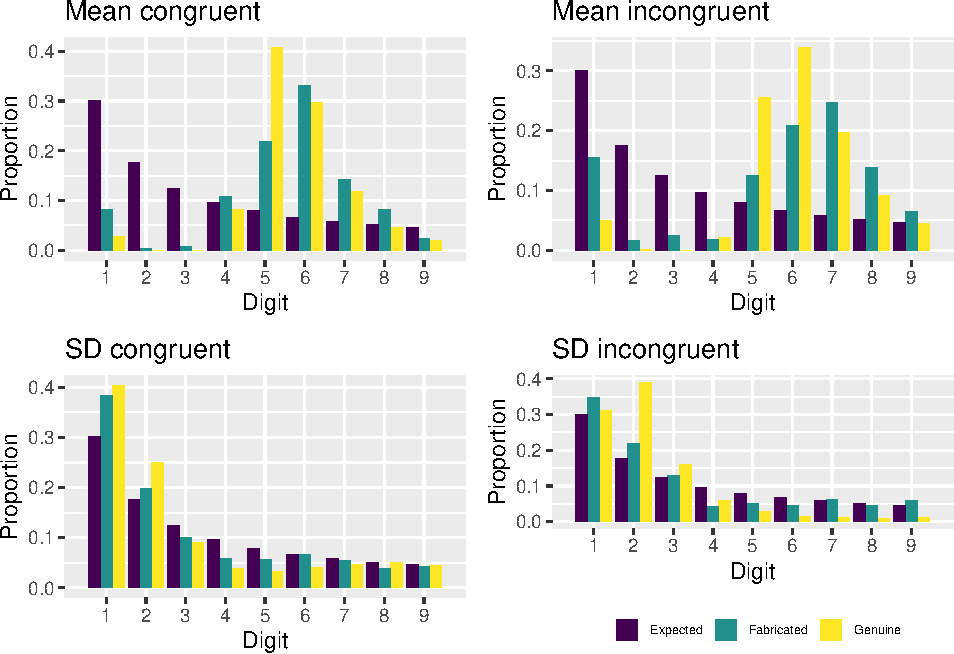
\includegraphics{_main_files/figure-latex/digit-nbl-1.pdf}
\caption{\label{fig:digit-nbl}First (Benford) digit distributions of the
(in)congruent means and standard deviations, aggregated across all Many
Labs 3 datasets, across the datasets fabricated by the participants, and
the theoretically expected proportions.}
\end{figure}

The AUROC results indicate that using the Newcomb-Benford Law is at best
on par with chance level classification of genuine and fabricated data.
More specifically, for the congruent standard deviations, using the
results of the NBL test are on par with chance classification
(\(AUROC=0.553\), 95\% CI {[}\(0.389\)-\(0.717\){]}). Using the
congruent standard deviations, we detected 19 of the 28 fabricated ones
as fabricated (\(\alpha=.01\)) and 13 of the 21 genuine ones as
fabricated (results per respondent available at
\href{https://osf.io/dsbge}{osf.io/dsbge}). Values from other measures
showcase that the fabricated data are actually \emph{more} in line with
the NBL than the genuine data. Consequently, the genuine data and
fabricated data are often wrongly classified. This is reflected by the
AUROC values that are significantly smaller than .5. For congruent
means, \(AUROC=0.039\), 95\% CI {[}\(0\)-\(0.087\){]}; Using the
congruent means, we detected 28 of the 28 fabricated ones as fabricated
(\(\alpha=.01\)) and 21 of the 21 genuine ones as fabricated (results
per respondent available at \href{https://osf.io/sgda8}{osf.io/sgda8}).
For incongruent means, \(AUROC=0.024\), 95\% CI {[}\(0\)-\(0.059\){]};
Using the incongruent means, we detected 28 of the 28 fabricated ones as
fabricated (\(\alpha=.01\)) and 21 of the 21 genuine ones as fabricated
(results per respondent available at
\href{https://osf.io/xjsd6}{osf.io/xjsd6}). For incongruent standard
deviations, \(AUROC=0.156\), 95\% CI {[}\(0.045\)-\(0.268\){]}; Using
the incongruent standard deviations, we detected 18 of the 28 fabricated
ones as fabricated (\(\alpha=.01\)) and 21 of the 21 genuine ones as
fabricated (results per respondent available at
\href{https://osf.io/2sd7w}{osf.io/2sd7w}).

Figure \ref{fig:digit-term} shows the aggregated terminal digit
distributions of the genuine and fabricated data side-by-side with the
expected terminal digit distributions. The first row depicts the
terminal digit distributions of the means, for both the congruent (left
column) and incongruent (right column) conditions. The first row shows
that the terminal digit distributions of the genuine and fabricated mean
response times are approximately uniform with only minor differences
between the genuine and fabricated data. The terminal digit
distributions of the standard deviations (second row) show slightly more
deviation from uniformly distributed digits, but still approximate the
expected distribution of terminal digits reasonably well. Based on these
aggregate digit distributions, it seems like the classification based on
the terminal digit analyses will not be able to differentiate between
genuine and fabricated data particularly well.

\begin{figure}
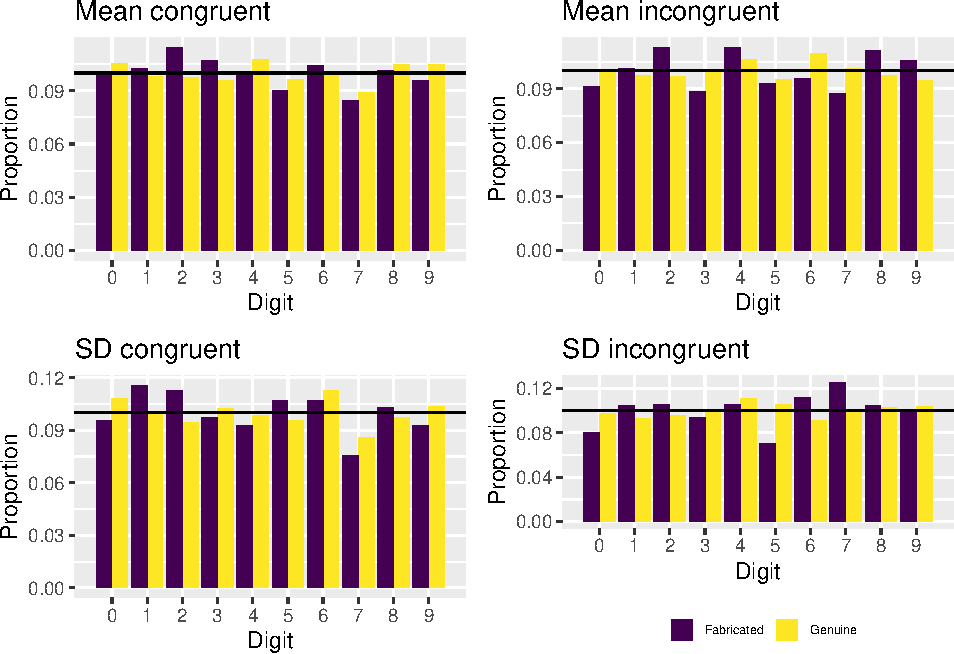
\includegraphics[width=1\linewidth]{_main_files/figure-latex/digit-term-1} \caption{Terminal digit distributions for the (in)congruent means and standard deviations, aggregated across all Many Labs 3 datasets or across the datasets fabricated by the participants.}\label{fig:digit-term}
\end{figure}

The AUROC results indeed show that terminal digit analyses perform close
to chance level classification of genuine and fabricated data. More
specifically, for the incongruent standard deviations, \(AUROC=0.511\),
95\% CI {[}\(0.343\)-\(0.679\){]}; congruent means, \(AUROC=0.383\),
95\% CI {[}\(0.222\)-\(0.543\){]}; incongruent means, \(AUROC=0.387\),
95\% CI {[}\(0.226\)-\(0.548\){]}; congruent standard deviations,
\(AUROC=0.401\), 95\% CI {[}\(0.241\)-\(0.562\){]}. The terminal digit
analysis classified at most 2 of the 28 fabricated datasets as being
fabricated (and 2 of the 21 genuine data as being fabricated;
\(\alpha=.05\)).

\subsubsection{Variance analysis}\label{variance-analysis-2}

Figure \ref{fig:sds-distribution} indicates that the standard deviations
of genuine data are larger on average and more dispersed. Results
indicate that the fabricated and genuine data can be perfectly separated
based on results from the variance analyses (\(max_z-min_z\)). More
specifically, the AUROC of both the variance analyses for the congruent
standard deviations and the incongruent standard deviations is
\(AUROC=1\) (confidence intervals cannot be reliably computed in this
case). We note that these results are likely to be sample specific and
do not mean to imply that this method will always be able to separate
the genuine- from fabricated data perfectly. However, they also indicate
that given the number of standard deviations participants had to
fabricate (\(k=25\)), it was difficult for participants to make them
look similar to those found in the genuine data. This method is
particularly difficult to apply if no reference distribution of
(arguably) genuine data is available.

\begin{figure}
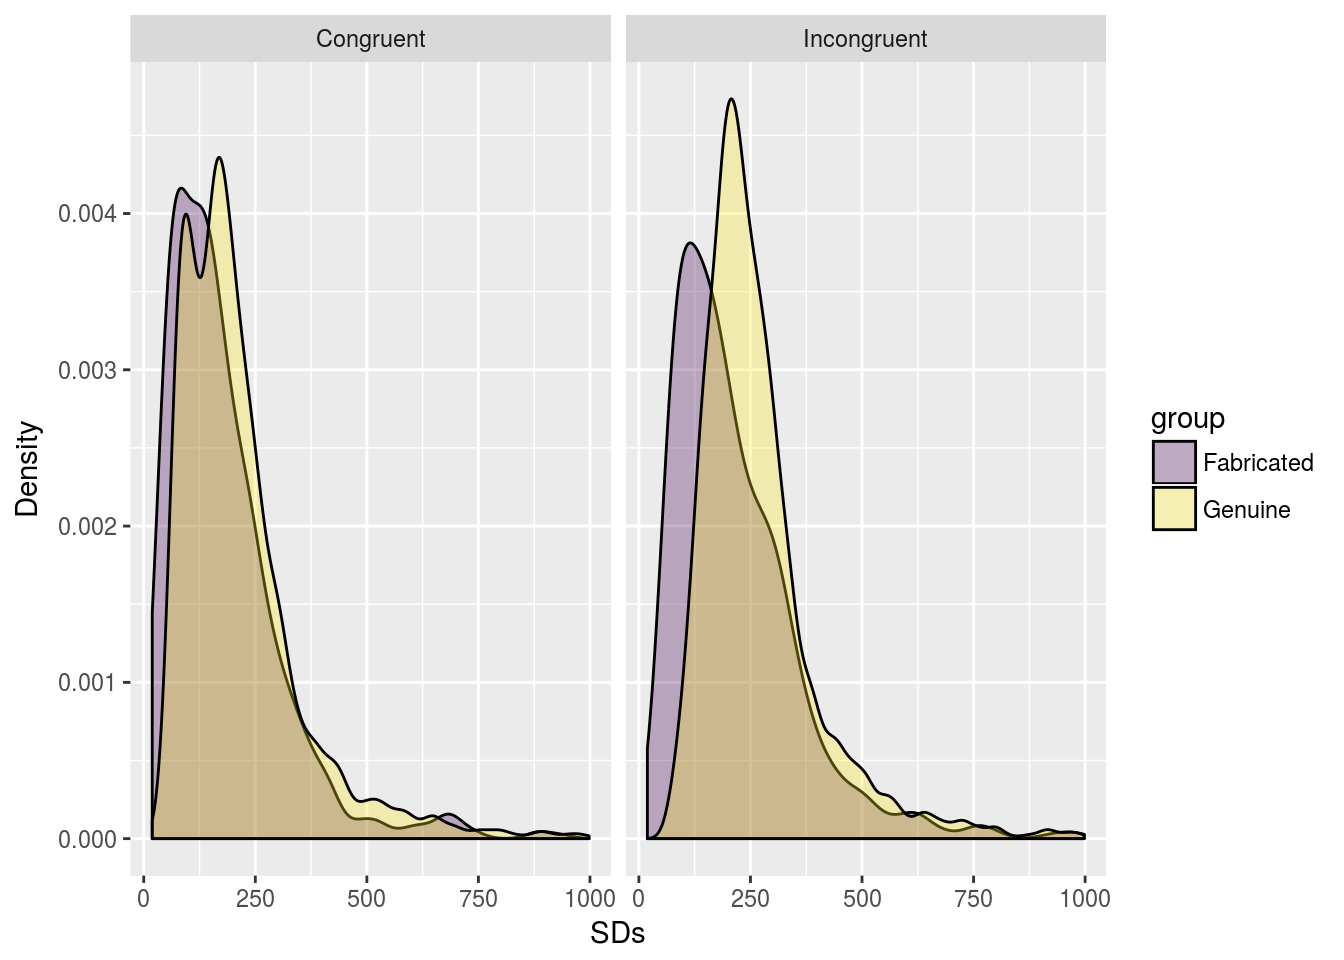
\includegraphics[width=1\linewidth]{_main_files/figure-latex/sds-distribution-1} \caption{Density distributions of the standard deviations of the response times in the congruent conditions (left) and the incongruent conditions (right), split for the genuine and fabricated data. X-axis truncated at 1000.}\label{fig:sds-distribution}
\end{figure}

Upon closer inspection of the individual level results of the variance
analyses per data set, all \(p\)-values are statistically significant if
compared to traditional \(\alpha\) levels (i.e., .05; maximum 0.006
across both the genuine- and the fabricated data). As a result, we
recommend that variance analyses are only used when a reference model is
available (in line with the results from Study 1).

\subsubsection{Multivariate
associations}\label{multivariate-associations-1}

We expected that fabricated multivariate associations would be different
from genuine multivariate associations. Using the parametric test of
multivariate associations, results indicate classification is fair to
good in the current sample. Figure \ref{fig:dens-mult} shows the density
distributions of the various multivariate associations (rows 1-2), which
already indicates that genuine data are less dispersed and more normally
distributed when compared to the fabricated multivariate associations.
Using the parametric estimates of the associations to test the various
sets of multivariate relations between the (in)congruent means and
standard deviations, \(AUROC\) values range from 0.549 through 0.842.
More specifically, the \(AUROC\) for the various sets of relations
(going clockwise with the first four figures in Figure
\ref{fig:dens-mult}) are \(AUROC=0.818\), 95\% CI
{[}\(0.689\)-\(0.947\){]} for \(M\)-\(SD\) in the congruent condition,
\(AUROC=0.833\), 95\% CI {[}\(0.705\)-\(0.962\){]} for \(M\)-\(SD\) in
the incongruent condition, \(AUROC=0.714\), 95\% CI
{[}\(0.568\)-\(0.861\){]} for \(M\)-\(M\) across conditions,
\(AUROC=0.549\), 95\% CI {[}\(0.379\)-\(0.72\){]} for \(SD\)-\(SD\)
across conditions. The percentage of fabricated multivariate relations
that is larger than all 21 genuine multivariate relations is 7.1\% for
\(M\)-\(SD\) congruent, 0\% for \(M\)-\(SD\) incongruent, 7.1\% for
\(M\)-\(M\) across, and 14.3\% for \(SD\)-\(SD\) across. Overall, it
seems that comparing multivariate associations to known genuine ones is
a good way to detect (potential) data fabrication, with the connotation
that a reference distribution is needed.

\begin{figure}
\centering
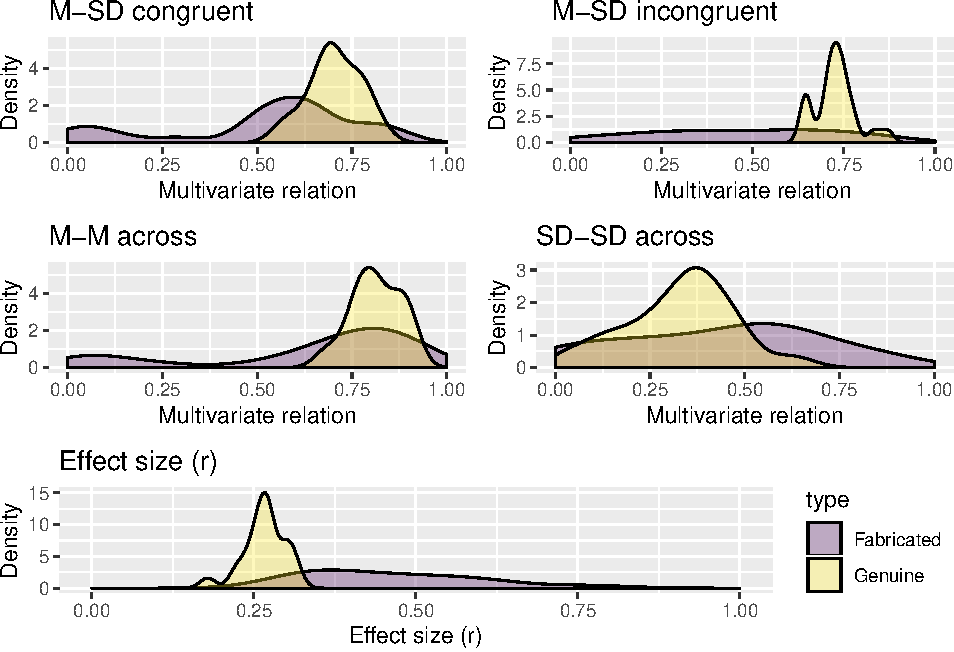
\includegraphics{_main_files/figure-latex/dens-mult-1.pdf}
\caption{\label{fig:dens-mult}Density distributions of the multivariate
relations (first two rows) and the effect sizes (final row), split for
the genuine and fabricated data.}
\end{figure}

\subsubsection{Combining variance, terminal digit, and associational
analyses}\label{combining-variance-terminal-digit-and-associational-analyses}

As preregistered, we combined both variance analyses, the terminal digit
analyses, and the tests of the multivariate associations with the Fisher
method (10 results in total). Results of the combined analysis perform
excellent at classifying fabricated and genuine data in this sample.
More specifically, the results for the combination method indicate
\(AUROC=0.959\) (95\% CI {[}\(0.912\)-\(1\){]}). This combination method
is affected by the effectiveness of the individual methods involved;
given that the performance of the multivariate associations and variance
analyses ranged from sufficient to excellent, it makes sense that this
combination method also performs quite well. The maximum \(p\)-value of
the combination of these tests for either the genuine or fabricated data
is 0.003 (results per respondent available at
\href{https://osf.io/rke9q}{osf.io/rke9q}), indicating that all datasets
would be classified as fabricated if we did not compare the results from
the genuine and fabricated data.

\subsubsection{Extreme effect sizes}\label{extreme-effect-sizes-2}

Figure \ref{fig:dens-mult} (final row) shows the density distributions
of the fabricated and genuine Stroop effect sizes, which is an excellent
classifier of fabricated/genuine data in this sample. More specifically,
the classification performance for detecting fabricated data in this
sample is \(AUROC=0.981\), 95\% CI {[}\(0.954\)-\(1\){]} (the 95\% CI is
truncated at 1), with fabricated effect sizes generally being larger
than genuine effect sizes. Upon closer inspection of the effect sizes,
we note that only three (of 28) fabricated effect sizes fall within the
range of genuine effect sizes (results per respondent available at
\href{https://osf.io/}{osf.io/}). As such, this is a particularly good
result within this sample (we did not preregister this analysis).

\subsubsection{Fabricating effects with Random Number Generators
(RNGs)}\label{fabricating-effects-with-random-number-generators-rngs-1}

Using Random Number Generators (RNGs) in the individual level data
fabrication procedure did not seem to have a substantial effect on how
genuine the fabricated results appeared. We explored this in our data
(i.e., not preregistered) and Table \ref{tab:rng2} presents the AUROC
values split on participating researchers who said they used (\(k=19\))
or did not use RNGs (\(k=9\)) to fabricate data (based on manual coding
of the interview transcripts). Noteworthy from our exploration is that
the effect size distribution seems approximately similar for both data
fabricated with and without RNGs (Figure \ref{fig:rng-mult2}). Given
these minor and inconsistent changes to the density distributions, we do
not regard RNGs as having substantial effects on the effectiveness of
statistical methods to detect data fabrication in this sample.

\begin{table}[!h]

\caption{\label{tab:rng2}AUROC values with 95 percent confidence intervals for each test, when split for those with Random Number Generators (RNGs) and those without.}
\centering
\resizebox{\linewidth}{!}{
\begin{tabular}{lll}
\toprule
Test & With RNG (k=19) & Without RNG (k=9)\\
\midrule
\rowcolor{gray!6}  Benford, congruent means & 0.035 [0-0.087] & 0.048 [0-0.144]\\
Benford, congruent sds & 0.506 [0.315-0.698] & 0.651 [0.431-0.87]\\
\rowcolor{gray!6}  Benford, incongruent means & 0.023 [0-0.064] & 0.026 [0-0.082]\\
Benford, incongruent sds & 0.115 [0.008-0.223] & 0.243 [0.015-0.472]\\
\rowcolor{gray!6}  Combination with Fisher method & 0.957 [0.9-1] & 0.963 [0.895-1]\\
\addlinespace
Effect size (r) & 0.985 [0.957-1] & 0.974 [0.918-1]\\
\rowcolor{gray!6}  Multivariate association, M-M across & 0.662 [0.481-0.842] & 0.825 [0.603-1]\\
Multivariate association, M-SD congruent & 0.85 [0.707-0.992] & 0.751 [0.488-1]\\
\rowcolor{gray!6}  Multivariate association, M-SD incongruent & 0.802 [0.637-0.967] & 0.899 [0.702-1]\\
Multivariate association, SD-SD across & 0.484 [0.272-0.695] & 0.688 [0.421-0.955]\\
\addlinespace
\rowcolor{gray!6}  Parametric test of Multivariate association, M-M across & 0.662 [0.481-0.842] & 0.825 [0.603-1]\\
Parametric test of Multivariate association, M-SD congruent & 0.85 [0.707-0.992] & 0.751 [0.488-1]\\
\rowcolor{gray!6}  Parametric test of Multivariate association, M-SD incongruent & 0.802 [0.637-0.967] & 0.899 [0.702-1]\\
Parametric test of Multivariate association, SD-SD across & 0.847 [0.717-0.977] & 0.831 [0.671-0.991]\\
\rowcolor{gray!6}  Terminal digits, congruent means & 0.388 [0.206-0.57] & 0.37 [0.132-0.609]\\
\addlinespace
Terminal digits, congruent sds & 0.439 [0.253-0.624] & 0.323 [0.087-0.559]\\
\rowcolor{gray!6}  Terminal digits, incongruent means & 0.36 [0.186-0.534] & 0.444 [0.181-0.708]\\
Terminal digits, incongruent sds & 0.573 [0.383-0.763] & 0.381 [0.162-0.6]\\
\rowcolor{gray!6}  Variance analysis, congruent sds (maxmin) & 1 [1-1] & 1 [1-1]\\
Variance analysis, incongruent sds (maxmin) & 1 [1-1] & 1 [1-1]\\
\bottomrule
\end{tabular}}
\end{table}

\begin{figure}
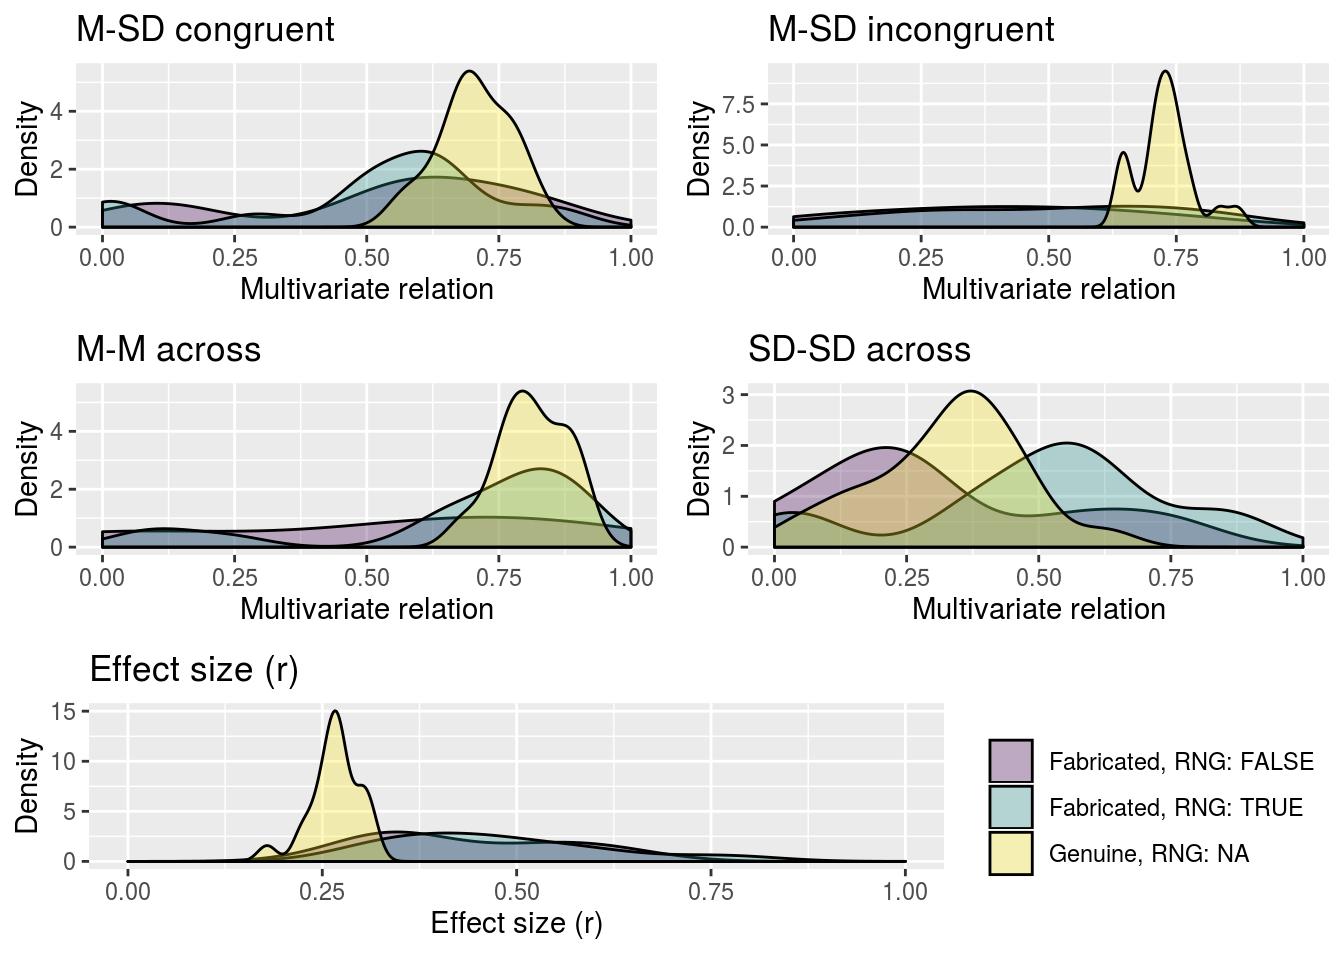
\includegraphics[width=1\linewidth]{_main_files/figure-latex/rng-mult2-1} \caption{Density distributions of the multivariate relations (first two rows) and the effect sizes (final row), split for the genuine data, the fabricated data without using Random Number Generators RNGs), and fabricated data with using RNGs.}\label{fig:rng-mult2}
\end{figure}

\subsection{Discussion}\label{discussion-5}

Our second study investigated how well statistical methods that use
individual-level (raw) data can distinguish fabricated data from genuine
data. To this end, we replicated the procedure from Study 1 and asked
researchers to fabricate data for individual participants for the
classic Stroop task. We also collected (arguably) genuine data from the
labs involved in the Many Labs study, which included the classic Stroop
task. As such, we had both genuine and fabricated data sets on the same
effect.

Using these data sets we attempted to classify genuine and fabricated
individual level data using digit analyses, variance analyses,
multivariate associations, and effect sizes. Results of preregistered
analyses indicate that digit analyses of raw data performed at chance
level, variance analyses of individual level data performed excellently,
and analyses of multivariate relations between variables in the
individual level data performed fairly to excellently. Moreover, the
summary statistic effect size appeared to strike a surprisingly good
balance between efficacy and parsimony for classifying fabricated- from
genuine individual level data (only superseded in performance by the
more complex variance analyses). This replicates the finding from Study
1 that effect sizes are a valuable piece of information to discern
genuine from fabricated data. Fabricators' use of Random Number
Generators (RNGs) did not appear to have a consistent relation with
classification performance with individual level data.

Our results confirmed our prediction that leading digit analyses (i.e.,
NBL) are not fruitful in detecting fabricated response times. The
Newcomb-Benford Law is frequently observed in various natural phenomena
(e.g., population numbers) but Figure \ref{fig:digit-nbl} (clearly)
indicates this is not the case for summary statistics of response times.
Response times are untruncated ratio measures in theory that technically
satisfy the NBL's requirements, but in practice response time measures
are truncated severely (e.g., nobody can respond within \textless{}50
milliseconds and few take longer than 2000 milliseconds). If the NBL is
being considered for applications to detect (potential) misconduct,
there need to be indications that the data generation process is in line
with the requirements of the NBL, but we consider that this is hardly
the case for experimental studies in the social sciences.

Going against our predictions, participants fabricated individual level
data that was almost indistinguishable from the genuine individual level
data when looking at terminal digit analyses. Given the theoretical
framework we use, wherein humans are expected to be poor at fabricating
stochastic processes that underlie data collection procedures, we
expected that our participants would be unable to fabricate uniformly
distributed terminal digits. Our sample indicates this is not the case.
Moreover, given that these stochastic processes are expected to be
better included when data is fabricated with RNGs, it was a surprise
that this did not affect classification performance. This raises
questions with respect to whether human's lack of intuitive
understanding of uniform probabilities manifests itself in fabricated
individual level data, and if so, under which conditions.

Study 2 replicated the effectiveness of variance analyses
(preregistered) and effect sizes (not preregistered) to detect data
fabrication, but failed to replicate the potential effect of RNGs on
detection rates (not preregistered). These mixed results with respect to
the effect of RNGs on the fabricated data suggests that a lack of
intuitions for probabilities does not necessarily manifest itself in
fabricated data. Hence, further research might look into correlating the
(lack of) expertise on probabilities and the kind of data being
fabricated. With respect to variance analyses and effect sizes, our
results suggest that these are the most promising methods when genuine
data are available (we further discuss this in the General Discussion).

Study 2 substantiates two conclusions from Study 1: (1) As methods may
not be robust to violations of its assumptions (e.g., NBL in Study 2),
these methods should be validated with genuine reference data if
available, before using these tools to flag potential problematic
papers. This dependence on assumptions also questions the validity of
automatic large-scale scrutiny for data fabrication. (2) Although some
methods did not perform well in Study 2, these methods have shown to
work well to detect data fabrication in some isolated cases of
misconduct. For instance, both the NBL (Cho and Gaines
\protect\hyperlink{ref-doi:10.2307ux2f27643897}{2007}) and the analysis
of terminal digits (Mosimann, Wiseman, and Edelman
\protect\hyperlink{ref-doi:10.1080ux2f08989629508573866}{1995}) have
shown their usefulness in some cases. Similarly, although some methods
worked well in Study 2 (i.e.~variance analyses, effect size
distributions, multivariate associations), this does not mean that they
always work well in detecting fabricated data, or that they could
exonerate anyone when these methods fail to flag any fabrication.

\section{General discussion}\label{general-discussion-1}

We presented the first two empirical studies on detecting individual
sets of fabricated data, where the fabricated data pertained to existing
experiments and detection occurred purely by using statistical methods.
By comparing results from genuine and fabricated data across summary
statistics and individual level data from two well-known psychology
research topics, it seems like classification based on statistically
significant effect sizes strikes the best balance between parsimony,
effectiveness, and usability. On the other hand, variance analyses are a
good option that is somewhat more complex in its application because one
has to identify the sets of variances that can be expected to be
homogeneous. The digit analyses based on the Newcomb-Benford law and the
terminal digit principle did not perform well. We bundled our functions
for the variance and digit analyses and the (reversed) Fisher method in
the \texttt{ddfab} (short for detecting data fabrication) package for
\texttt{R}, which is available through GitHub
(\url{https://github.com/chartgerink/ddfab}) for application in further
research and development.

We designed the current studies to have sufficient information to detect
data fabrication within a given set of data, but not necessarily to
generalize our results to a larger population. As such, the sample sizes
of the presented studies and the type of effect we chose as the
empirical context necessarily restrict the drawing of more general
inferences. Further research should consider whether these results also
apply to other types of data or effects. Nevertheless, our studies have
highlighted that variance- and effect size analysis and multivariate
associations are methods that look promising to detect problematic data.
Our descriptive results with confidence intervals may be regarded as an
initial step in understanding the effectiveness of these methods to
detect data fabrication (although we note those of the Fisher method are
incorrect due to dependent \(p\)-values). Next, we highlight some of the
difficulties that remain.

All presented results throughout the two studies pertain to relative
comparisons between genuine and fabricated data. Hence, all statements
about the performance of classification depends on the availability of
unbiased genuine data to compare to and cannot readily be done by using
generic decision criteria such as \(\alpha\)-levels. As we saw for
example in the variance analyses for Study 2, there was excellent
relative classification, but absolute classification as many researchers
are used to by comparing \(p<\alpha\) remained impossible or problematic
at best. More specifically, we would have classified all datasets as
fabricated if we had used the traditional hypothesis testing approach.
Hence, we agree with the call to always include a control sample when
applying these statistical tools to studies that look suspicious
(Simonsohn
\protect\hyperlink{ref-doi:10.1177ux2f0956797613480366}{2013}). It is
for exactly this reason that we refrain from formulating general
decision rules for the methods presented in this paper. This might also
have implications for systematic applications of statistical methods to
detect potentially problematic data, such as the recent application by
Carlisle
(\protect\hyperlink{ref-doi:10.1111ux2fanae.13938}{2017}\protect\hyperlink{ref-doi:10.1111ux2fanae.13938}{a}).
Carlisle
(\protect\hyperlink{ref-doi:10.1111ux2fanae.13938}{2017}\protect\hyperlink{ref-doi:10.1111ux2fanae.13938}{a})
used the same method applied in the Fujii case to approximately 5,000
clinical trials without any further validation of the methods (Bolland
et al.
\protect\hyperlink{ref-doi:10.1016ux2fj.jclinepi.2019.03.001}{2019}).
Our results suggest that in practice aberrant effects are best detected
in relative fashion, for example in a meta-analysis (corroborating our
own anecdotal experience), or to look for excessively large effect sizes
(e.g., \(r>.95\)) as an initial screening of a set of effects
(especially when that effect size is larger than the reliability of the
product of the measures involved). Using absolute classification (i.e.,
\(p<\alpha\)) can be problematic, considering that many of the methods
we tested (e.g., variance analyses, digit analyses) are not specific
enough and rely on models with strong assumptions, potentially flagging
both genuine and fabricated data as problematic.

Because we included the Many Labs data (R. A. Klein et al.
\protect\hyperlink{ref-doi:10.1027ux2f1864-9335ux2fa000178}{2014};
Ebersole et al.
\protect\hyperlink{ref-doi:10.1016ux2fj.jesp.2015.10.012}{2016}) we had
(arguably) unbiased estimates of the effects under investigation, which
is key for relative comparisons. If we had used the peer-reviewed
literature on the anchoring effect (Study 1) or the Stroop effect (Study
2), we would likely have found inflated effect size estimates of the
anchoring- or Stroop effects due to publication bias. These inflated
effect size estimates could have resulted in worsened classification of
genuine and fabricated data because publication bias results in inflated
effect sizes (Nuijten, Van Assen, et al.
\protect\hyperlink{ref-doi:10.1037ux2fgpr0000034}{2015}) and our studies
indicate fabricating data has a similar effect. That publication bias
and fabricating data might have similar effects in turn conflates the
detection of fabricated data. Collecting an unbiased genuine effect
distribution thus requires careful attention; when arguably genuine
effects are collected from a literature ridden with publication bias and
related biases, detection of data fabrication may be undermined. We
recommend retrieving unbiased effect size distributions for an effect
from large-scale replication projects, such as Registered Replication
Reports (e.g., Cheung et al.
\protect\hyperlink{ref-doi:10.1177ux2f1745691616664694}{2016}) and
building systemic efforts to reduce publication bias (see also
Hartgerink and Zelst
\protect\hyperlink{ref-doi:10.3390ux2fpublications6020021}{2018}).

Our results depend on the (majority of the) Many Labs data being
genuine. We remain confident that (most of) the Many Labs data are
genuine for a variety of reasons. First, the sheer number of people
involved in these projects results in a distribution of responsibility
that also limits the effect if one person were to fabricate data.
Second, the number of people involved also minimizes the individual
reward it would have to fabricate data given that any utility would have
to be shared across all researchers involved. Third, the projects
actively made all individual research files available and participating
researchers in the ML were made aware of this from the very start.
Fourth, the analyses of the Many Labs are not conducted by the same
individuals who collected the data. We of course cannot exclude the
possibility of malicious actors in the ML studies, but also have no
evidence that suggests there would be.

Highly relevant to the application of these kinds of methods in
screening for problems in the published literature (e.g., Bik,
Casadevall, and Fang
\protect\hyperlink{ref-doi:10.1128ux2fmBio.00809-16}{2016}\protect\hyperlink{ref-doi:10.1128ux2fmBio.00809-16}{b};
Carlisle
\protect\hyperlink{ref-doi:10.1111ux2fanae.13938}{2017}\protect\hyperlink{ref-doi:10.1111ux2fanae.13938}{a})
or during peer review is that the diagnostic value of any instrument is
dependent on the base rate of afflicted cases (here: fabricated data).
In our study design, we built in a high prevalence of data fabrication,
which directly affects the positive predictive value of these
statistical methods. The positive predictive value is the chance of
getting a true positive when a positive result is found. More
specifically, Study 1 by design has a prevalence of 52\% of data
fabrication and Study 2 has a prevalence of 57\%. This strongly affects
the positive predictive value (PPV) of these methods if they would be
applied in a more general setting. After all, even if we could classify
all fabricated data correctly and falsely regard genuine data as
fabricated in 5\% of the cases, then with a prevalence of 2\% (Fanelli
\protect\hyperlink{ref-doi:10.1371ux2fjournal.pone.0005738}{2009}) the
positive predictive value would only be 29\%. This is a best-case
scenario (see also Stricker and Günther
\protect\hyperlink{ref-doi:10.1027ux2f2151-2604ux2fa000356}{2019}) that
would cause approximately 1 out of 3 cases of \enquote{detected data
fabrication} to be false. Hence, we do not recommend attempting to
detect data fabrication on statistical methods alone.

We do advise to use some of the more successful statistical methods as
screening tools in review processes and as additional tools in formal
misconduct investigations where prevalence is supposedly higher than in
the general population of research results. We note that this should
only happen in combination with evidence from other sources than
statistical methods (e.g., focusing on practical, methodological, or
substantive aspects). As we mentioned before, excessively large effect
sizes might be used as a screening approach for further manual or
in-depth investigation, but we warn against the potential for
confirmation bias that results from these earlier tests might create. As
such, if any of these statistical tools are used, we recommend to solely
use them to screen for indications of potential data anomalies, which
are subsequently further inspected by a blinded researcher to prevent
confirmation bias and using a rigorous protocol that involves due care
and due process.

We note that our studies have been regarded as unethical by some due to
the nature of asking participants to fabricate data (see for example
Ellemers \protect\hyperlink{ref-ellemers}{2017}). We understand and
respect that asking researchers to show one of the most widely condemned
scientific behaviors is risky. While designing these studies, we also
asked ourselves whether this was an appropriate design and ultimately
regarded it was appropriate for several reasons. First, there was little
utility in simulating potential data fabrication strategies because
there is little to no knowledge of how researchers actually fabricate
data. Second, the cases of data fabrication known to us are severely
self-selected (i.e., based on detection bias), which would limit the
ecological validity of any tests we could do on such suspect data. These
two reasons made it necessary for us to collect fabricated data. After
we had come to that decision, we also regarded that we should minimize
the negative effect it had on the researchers participating. We
attempted to minimize any negative effect by using findings from
psychology research to decrease potential carry-over of this controlled
misbehavior (Mazar, Amir, and Ariely
\protect\hyperlink{ref-doi:10.1509ux2fjmkr.45.6.633}{2008}; although a
recent multilab replication contested this effect, Verschuere et al.
\protect\hyperlink{ref-doi:10.1177ux2f2515245918781032}{2018}). Despite
that some of our participants indicated that they felt initial unease
with fabricating data for the study, no participants reached out
afterwards indicating feeling conflicted. Moreover, we actively attempt
to maximize returns of the data collected by sharing all the information
we gathered openly and without restrictions. We consider these reasons
to balance the design and ask of our study from our participants.

Another ethical issue is the dual use of these kinds of statistical
methods to detect data fabrication. Dual use is the ethical issue where
the development of knowledge can be used for both good and evil
purposes, hence, whether we should want to morally conduct this
research. A traditional example is the research into biological agents
that might be used for chemical warfare. For our research, a data
fabricator might use our research to test their fabricated data until it
goes undetected based on these methods. There is no inherent way to
control whether malicious actors do this and one might argue that this
is sufficient reason to shy away from conducting this kind of research
to begin with. However, we argue that the potential ethical uses of
these methods are substantial (improved detection of fabricated data by
a potential many) and outweigh the potential unethical uses of these
methods (undermining detection by a potential few). Secrecy in this
respect would actually enhance the ability of malicious actors to remain
undetected, because when they find a way to exploit the system fewer
people can investigate suspicions they might have. Hence, we regard the
ethical issue of dual use to ultimately weigh in favor of doing the
research, although we recognize that this might start a competition in
undermining detection of problematic data.

Some of our participants in Study 2 indicated using the Many Labs (or
other open) data to fabricate their own dataset. During the interviews,
some participants indicated that they thought this would make it more
difficult to detect their data as fabricated. We did not investigate
evidence for this claim specifically (this could be avenue for further
research) but we note that our detection in Study 2 performed well
despite some participants using genuine data. Moreover, we note that
open data might actually facilitate the detection of fabricated data for
two reasons. First, open data from preregistered projects improves the
unbiased estimation of effect sizes and multivariate associations, where
the peer-reviewed literature inflates estimated effect sizes due to
publication bias and often lacks the required information to compute
these multivariate associations. As we mentioned before, having these
unbiased effect size estimates seem key to detecting issues. Second, if
data are fabricated based on existing data, it is more likely to be
detected if it is based on open data than when based on closed data. For
example, in the LaCour case data were fabricated based on existing data
(McNutt \protect\hyperlink{ref-doi:10.1126ux2fscience.aac6184}{2015};
LaCour and Green
\protect\hyperlink{ref-doi:10.1126ux2fscience.1256151}{2014}).
Researchers detected that this data had been fabricated because it
seemed to be a(n almost) linear transformation of variables because they
could access the relevant dataset (Broockman, Kalla, and Aronow
\protect\hyperlink{ref-lg-irreg}{2015}). As such, we see no concrete
evidence to support the claim that open data could lead to worsened
detection of fabricated data, but we also recognize that this does not
exclude it as an option. As such, beyond being fruitful for examining
reproducibility (Munafò et al.
\protect\hyperlink{ref-doi:10.1038ux2fs41562-016-0021}{2017}) and
facilitating new research, open data may also facilitate the improvement
of detecting potential data fabrication. We see the effect of open data
on detection of data fabrication as a fruitful avenue for further
research.

All in all, we see a need for unbiased effect size estimates to provide
meaningful comparisons of genuine- and potentially fabricated data, but
even when those are available the (potentially) low positive predictive
value of widespread detection of data fabrication is going extremely
difficult. Hence, we recommend meta-research to focus on more effective
systemic reforms to make progress on the root causes of data fabrication
possible. One root cause is likely to be the incentive system that
rewards bean-counts of outputs and does not put them in the context of a
larger collective scientific effort where validity counts. Our premise
in these two research studies was after the fact detection of a problem,
but we recognize that prior to the fact addressing of the underlying
causes that give rise to data fabrication is more sustainable and
effective. Nonetheless, we also recognize that there will always be
dishonesty involved for some researchers, and we recommend that research
engage in more penetration testing of how those with dishonesty can fool
a system.

\part{Improving science}\label{part-improving-science}

\chapter{Extracting data from vector figures in scholarly
articles}\label{extracting-data-from-vector-figures-in-scholarly-articles}

It is common for authors to communicate their results in graphical
figures, but what is generally not realised it that it may be possible
to reconstruct the original data from a data based figure (see also the
preceding ``In Brief'' report; Hartgerink
\protect\hyperlink{ref-Hartgerink-dlib2017}{2017}\protect\hyperlink{ref-Hartgerink-dlib2017}{a}).
Figures are typically presented in order to communicate something about
the underlying data, but in an inherently static way. As such, reshaping
this communication is not readily possible, because the original data
are not available. Examples of reuse if the data are available could be
as simple as joining data across figures, standardizing axes across
figures for easy comparison, changing color codings to be more
colorblind friendly, or using the data to compute relative numbers
instead of absolute numbers. Moreover, considering the current low rates
of data sharing (Wicherts et al.
\protect\hyperlink{ref-doi:10.1037ux2f0003-066x.61.7.726}{2006};
Vanpaemel et al.
\protect\hyperlink{ref-doi:10.1525ux2fcollabra.13}{2015}; Krawczyk and
Reuben
\protect\hyperlink{ref-doi:10.1080ux2f08989621.2012.678688}{2012}) and
rapid decrease of the odds of successfully requesting those data (Vines
et al. \protect\hyperlink{ref-doi:10.1016ux2fj.cub.2013.11.014}{2014}),
reusing data effectively becomes impossible in the long run because data
simply are not available any more. Hence, we find it important to be
able to have alternative ways of extracting data solely from results
presented in a scholarly report.

Some figures are stored in bitmap format whereas others are stored in
vector format. In a bitmap format the image is stored by saving the
color code for each pixel. This means that information about overlapping
datapoints is lost, because a pixel in a bitmap does not differentiate
between different layers. However, in a vector format, information is
stored on the shape and its position on the canvas, which is
unrestricted to a specific pixel size, and information can be saved. As
such, these images can be enlarged without loss of image quality.
Moreover, the position of those shapes can be retraced in order to
reconstruct data points in a figure. This can even be done when data
points overlap, because unlike in the pixel format, overlapping shapes
are stored alongside each other in a vector image.

To extract data points manually from a figure, an author may have to
measure the coordinates either on printed pages using a ruler, or from
the display screen using a cursor. This is time-consuming (often hours)
and error-prone, and limited by the precision of the display or ruler.
What is often not realised is that the data themselves are held in the
PDF document to much higher precision (usually 0.0-0.01 pixels), if the
figure is stored in vector format. By using suitable software we can
extract the coordinates of the individual data points without ambiguity
or loss of inherent precision. For example, a figure with 10,000
\emph{x}-values presented onto 500 pixels will suffer massive overlap in
the display but all 10,000 data points are recoverable from the PDF if
the figure is stored in vector format.

In the current report, we share the results of the alpha software
\texttt{norma}
(\href{https://github.com/contentmine/norma}{github.com/contentmine/norma})
to automatically extract raw data from vector based figures. More
specifically, we report the method of data extraction, the
effectiveness, and provide documentation to use the software pipeline.
Finally, we review the potential of using vector based images to extract
data from scholarly reports in light of the results.

\section{Method}\label{method-3}

\hypertarget{extraction-procedure}{\subsection{Extraction
procedure}\label{extraction-procedure}}

At the highest level, typical figure components are the body, header,
footer, and axes. Figure \ref{fig:vector-fig1} provides a visual
depiction of these figure components. In order to extract data,
recognition of some these components is mandatory, whereas recognition
of others is optional. For example, the header and footer are irrelevant
to data extraction, but are relevant to data comprehension; hence these
are optional. Left- and bottom axes are mandatory, because these
typically depict the scale of the presented plots. Right- and top axes
are optional because they are rarely used as the main axes and mostly
just to delimit the plotbox (as far as we know). Logically, the body of
the plot, containing the depicted data, is mandatory for data
extraction.

\begin{figure}

{\centering 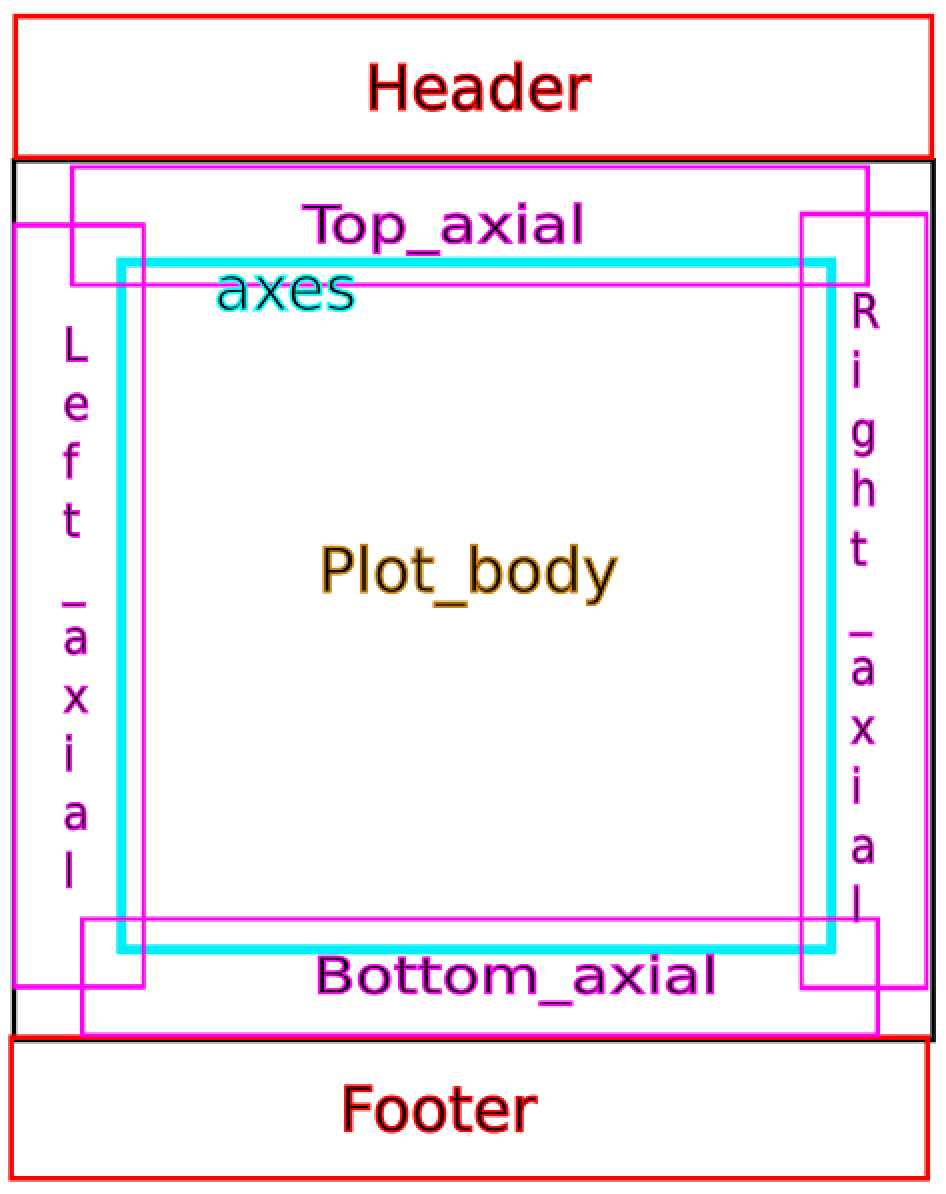
\includegraphics[width=0.4\linewidth]{assets/figures/plot-components} 

}

\caption{Visual representation of the typical components to a data based plot. This serves as the basis of the software to extract data from the plot body.}\label{fig:vector-fig1}
\end{figure}

Based on the plot body, absolute locations of the individual data points
are extracted. Not all vector images are created in a similar way, but
in the simplest scenario with data points depicted as circles, the
vector gives three parameters: the \(x\) coordinate of the centre, the
\(y\) coordinate of the centre, and the radius \(r\). As such, for a
simple circle the underlying vector code (in Scalable Vector Graphics,
SVG) might look as follows:

\begin{Shaded}
\begin{Highlighting}[]
\KeywordTok{<circle}\OtherTok{ cx=}\StringTok{"103.71"}\OtherTok{ cy=}\StringTok{"121.22"}\OtherTok{ r=}\StringTok{"25.234"}\OtherTok{ fill-opacity=}\StringTok{"0"}
\OtherTok{        stroke=}\StringTok{"#cf1d35"} 
\OtherTok{        stroke-width=}\StringTok{".26458"}\KeywordTok{/>}
\end{Highlighting}
\end{Shaded}

This information can be readily extracted after isolating the vector
figure from a PDF file. The current alpha software is primarily
developed to operate on circles of similar size within one plot but can
be extended for data depicted in other ways.

In order to make the absolute locations of the shapes represent the
original data points as accurately as possible, they are mapped onto the
identified x- and y-axis. Although absolute locations retain the
relative relations between the individual data points, they are not
representative of the original data. \texttt{norma} interprets
characters as \enquote{ladders} of numeric values along the axes. It
then identifies a rectangular box, examines it for tick marks and
matches the ticks to the axial scale values. Subsequently, the location
of the data on the x-axis and y-axis are combined with the information
about the scale in order to remap the absolute locations of the points
on the canvas into the original data points. The current alpha software
assumes a linear scale, but logarithmic scales could be incorporated at
a future stage.

\subsection{Corpus}\label{corpus}

Using ScienceOpen, we searched for meta-analytic reports that mention
\enquote{publication bias}. For this project, we focused on funnel plot
figures from meta-analyses. We restricted our search on ScienceOpen to
Open Access reports, in order to legally redistribute those reports in
the \href{https://github.com/chartgerink/2015ori-3}{Github project
repository (https://github.com/chartgerink/2015ori-3)}, which
facilitates reproducibility of our procedure. We searched the
ScienceOpen database on March 30 2017; this search resulted in 422
reports (see also Figure \ref{fig:vector-fig2}), but the webpage
presented only 368 reports.

\begin{figure}
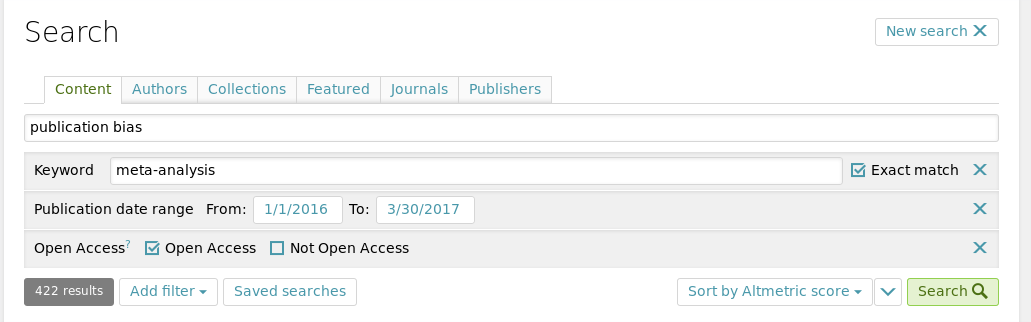
\includegraphics[width=1\linewidth]{assets/figures/search-results} \caption{Screenshot of the search criteria used to search ScienceOpen.}\label{fig:vector-fig2}
\end{figure}

We manually searched through these 368 reports for vector based funnel
plots. The first author (CHJH) checked each article for (1) whether a
funnel plot was present; (2) if so, how many funnels were present, and
(3) whether the funnel plots were vector based. In order to determine
whether a funnel plot was vector based, a heuristic was used. This
heuristic was to try and select the axes (either x- or y-axis) from the
plot. If we could select the labels from the tickmarks, the plot was
deemed to be vector based, otherwise it was dropped. We later found out
this was a liberal heuristic, considering some publishers present vector
axes but incorporate a bitmap plot body (see Figure
\ref{fig:vector-fig3} for an example).

\begin{figure}[h]
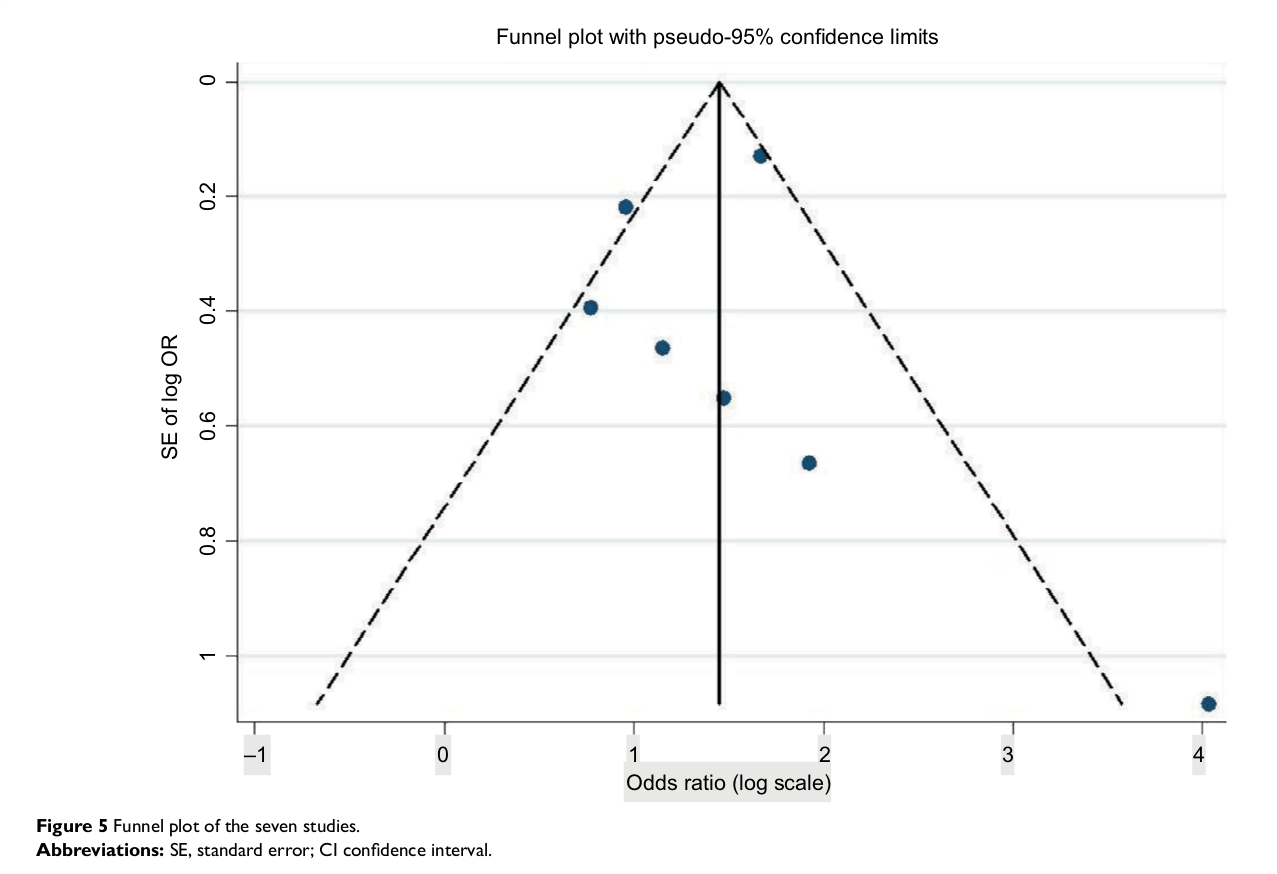
\includegraphics[width=1\linewidth]{assets/figures/example-bitmap} \caption{Example of a funnel plot with selectable axes, but including a bitmap body. This can be seen by the large difference in quality between the body and the axes, where the axes are crisp and the body is pixelated. The x-axis is selected. Funnel plot reproduced under CC BY-NC license from 10.2147/amep.s116699.}\label{fig:vector-fig3}
\end{figure}

\subsection{Documentation}\label{documentation}

The following documentation assumes that the Github repository for this
project is cloned and that the working directory is the resulting
folder. As such, in order to walk through these documentation steps, the
following code is run from the shell command line

\begin{Shaded}
\begin{Highlighting}[]
\CommentTok{# Via SSH}
\FunctionTok{git}\NormalTok{ clone git@github.com:chartgerink/2015ori-3}
\CommentTok{# Via HTTPS (if you don't know what SSH is, use this)}
\FunctionTok{git}\NormalTok{ clone https://github.com/chartgerink/2015ori-3}
\CommentTok{# Change the working directory}
\BuiltInTok{cd}\NormalTok{ 2015ori-3}
\end{Highlighting}
\end{Shaded}

If \texttt{git} is not available from the commandline, a direct download
of the project is available from Github
(\url{https://github.com/chartgerink/2015ori-3/archive/master.zip}). All
other dependencies to reproduce the results are included in the packaged
command line tool \texttt{norma} and the user is only required to have
Java installed on their system and available from the commandline.

In order to extract data from vector figures with the software
\texttt{norma}, 5 steps are taken. First, the user needs to organize all
original PDFs into one folder. Second, this folder needs to be converted
to a \texttt{cproject} structure. The \texttt{cproject} structure
normalizes the contents for each paper into a \texttt{ctree}, such that
subsequent operations are trivial to standardize (and extensions can be
applied relatively easily). For example, the root folder might contain
\texttt{ctree1.pdf}, but after transforming the root folder into a
\texttt{cproject} it contains a folder \texttt{ctree1/} with
\texttt{fulltext.pdf}. By running the command

\begin{Shaded}
\begin{Highlighting}[]
\ExtensionTok{java}\NormalTok{ -jar bin/norma-0.5.0-SNAPSHOT-jar-with-dependencies.jar \textbackslash{}}
\NormalTok{  --project corpus-raw \textbackslash{}}
\NormalTok{  --fileFilter }\StringTok{'.*/(.*).pdf'}\NormalTok{ \textbackslash{}}
\NormalTok{  --makeProject }\StringTok{'(\textbackslash{}1)/fulltext.pdf'}
\end{Highlighting}
\end{Shaded}

the folder \texttt{corpus-raw} (\texttt{-\/-project\ corpus-raw}) is
restructured into a \texttt{cproject} structure, containing a folder for
each PDF file
(\texttt{-\/-fileFilter\ \textquotesingle{}.*/(.*).pdf\textquotesingle{}\ -\/-makeProject\ \textquotesingle{}(\textbackslash{}1)/fulltext.pdf\textquotesingle{}}).
This results in the following folder structure, where
\texttt{fulltext.pdf} is the original PDF and \texttt{ctree1} (etc.) may
capture the DOI or other document identifiers.:

\begin{Shaded}
\begin{Highlighting}[]
\ExtensionTok{cproject/}
\KeywordTok{|}\ExtensionTok{---}\NormalTok{ ctree1}
\KeywordTok{|}   \KeywordTok{|}\ExtensionTok{---}\NormalTok{ fulltext.pdf}
\KeywordTok{|}\ExtensionTok{---}\NormalTok{ ctree2}
\KeywordTok{|}   \KeywordTok{|}\ExtensionTok{---}\NormalTok{ fulltext.pdf}
\ExtensionTok{...}
\KeywordTok{|}\ExtensionTok{---}\NormalTok{ ctreeN}
    \KeywordTok{|}\ExtensionTok{---}\NormalTok{ fulltext.pdf}
\end{Highlighting}
\end{Shaded}

After converting the folder into a \texttt{cproject}, the \texttt{norma}
software is applied to convert the PDF files into separate SVGs per
page. In order to convert each page of the PDF into a separate SVG file,
we used the following command

\begin{Shaded}
\begin{Highlighting}[]
\ExtensionTok{java}\NormalTok{ -jar bin/norma-0.5.0-SNAPSHOT-jar-with-dependencies.jar \textbackslash{}}
\NormalTok{  --project corpus-raw \textbackslash{}}
\NormalTok{  -i fulltext.pdf --outputDir corpus-raw --transform pdf2svg}
\end{Highlighting}
\end{Shaded}

resulting in a \texttt{svg/} folder for each \texttt{ctree} in the
structure presented above. That is, each \texttt{ctree} now contains a
folder with one vector file for each page in the fulltext PDF.

The following step, extracting the plots from the page and saving these,
currently needs to be done manually. We recommend using the FOSS
software \href{https://inkscape.org/}{Inkscape} to do this. For each
article, open the pages containing funnel plots, select the area of the
plot, and press the keyboard shortcut \texttt{SHIFT+1} (i.e.,
\texttt{!}) to inverse the selection; then press the \texttt{delete} key
to retain only the plot. Subsequently save the file as
\texttt{Plain\ SVG} (not \texttt{Inkscape\ SVG}) and structure the
folders as follows:

\begin{Shaded}
\begin{Highlighting}[]
\ExtensionTok{cproject/}
\KeywordTok{|}\ExtensionTok{---}\NormalTok{ ctree1}
    \KeywordTok{|}\ExtensionTok{---}\NormalTok{ fulltext.pdf}
    \KeywordTok{|}\ExtensionTok{---}\NormalTok{ figures/}
        \KeywordTok{|}\ExtensionTok{---}\NormalTok{ figure1/}
            \KeywordTok{|}\ExtensionTok{---}\NormalTok{ figure.svg}
        \KeywordTok{|}\ExtensionTok{---}\NormalTok{ figure2/}
            \KeywordTok{|}\ExtensionTok{---}\NormalTok{ figure.svg}
\end{Highlighting}
\end{Shaded}

where \texttt{figure1} contains the first funnel plot (not the figure
number in the paper), \texttt{figure2/} contains the second funnel plot,
etc. If a figure is contained in a box, it is important to retain only
the figure and exclude the box (see Figure \ref{fig:vector-fig4} for an
example). In the Github repository, we provide a project folder that
already contains all the clipped images for the corpus under
investigation in this chapter.

\begin{figure}[h]
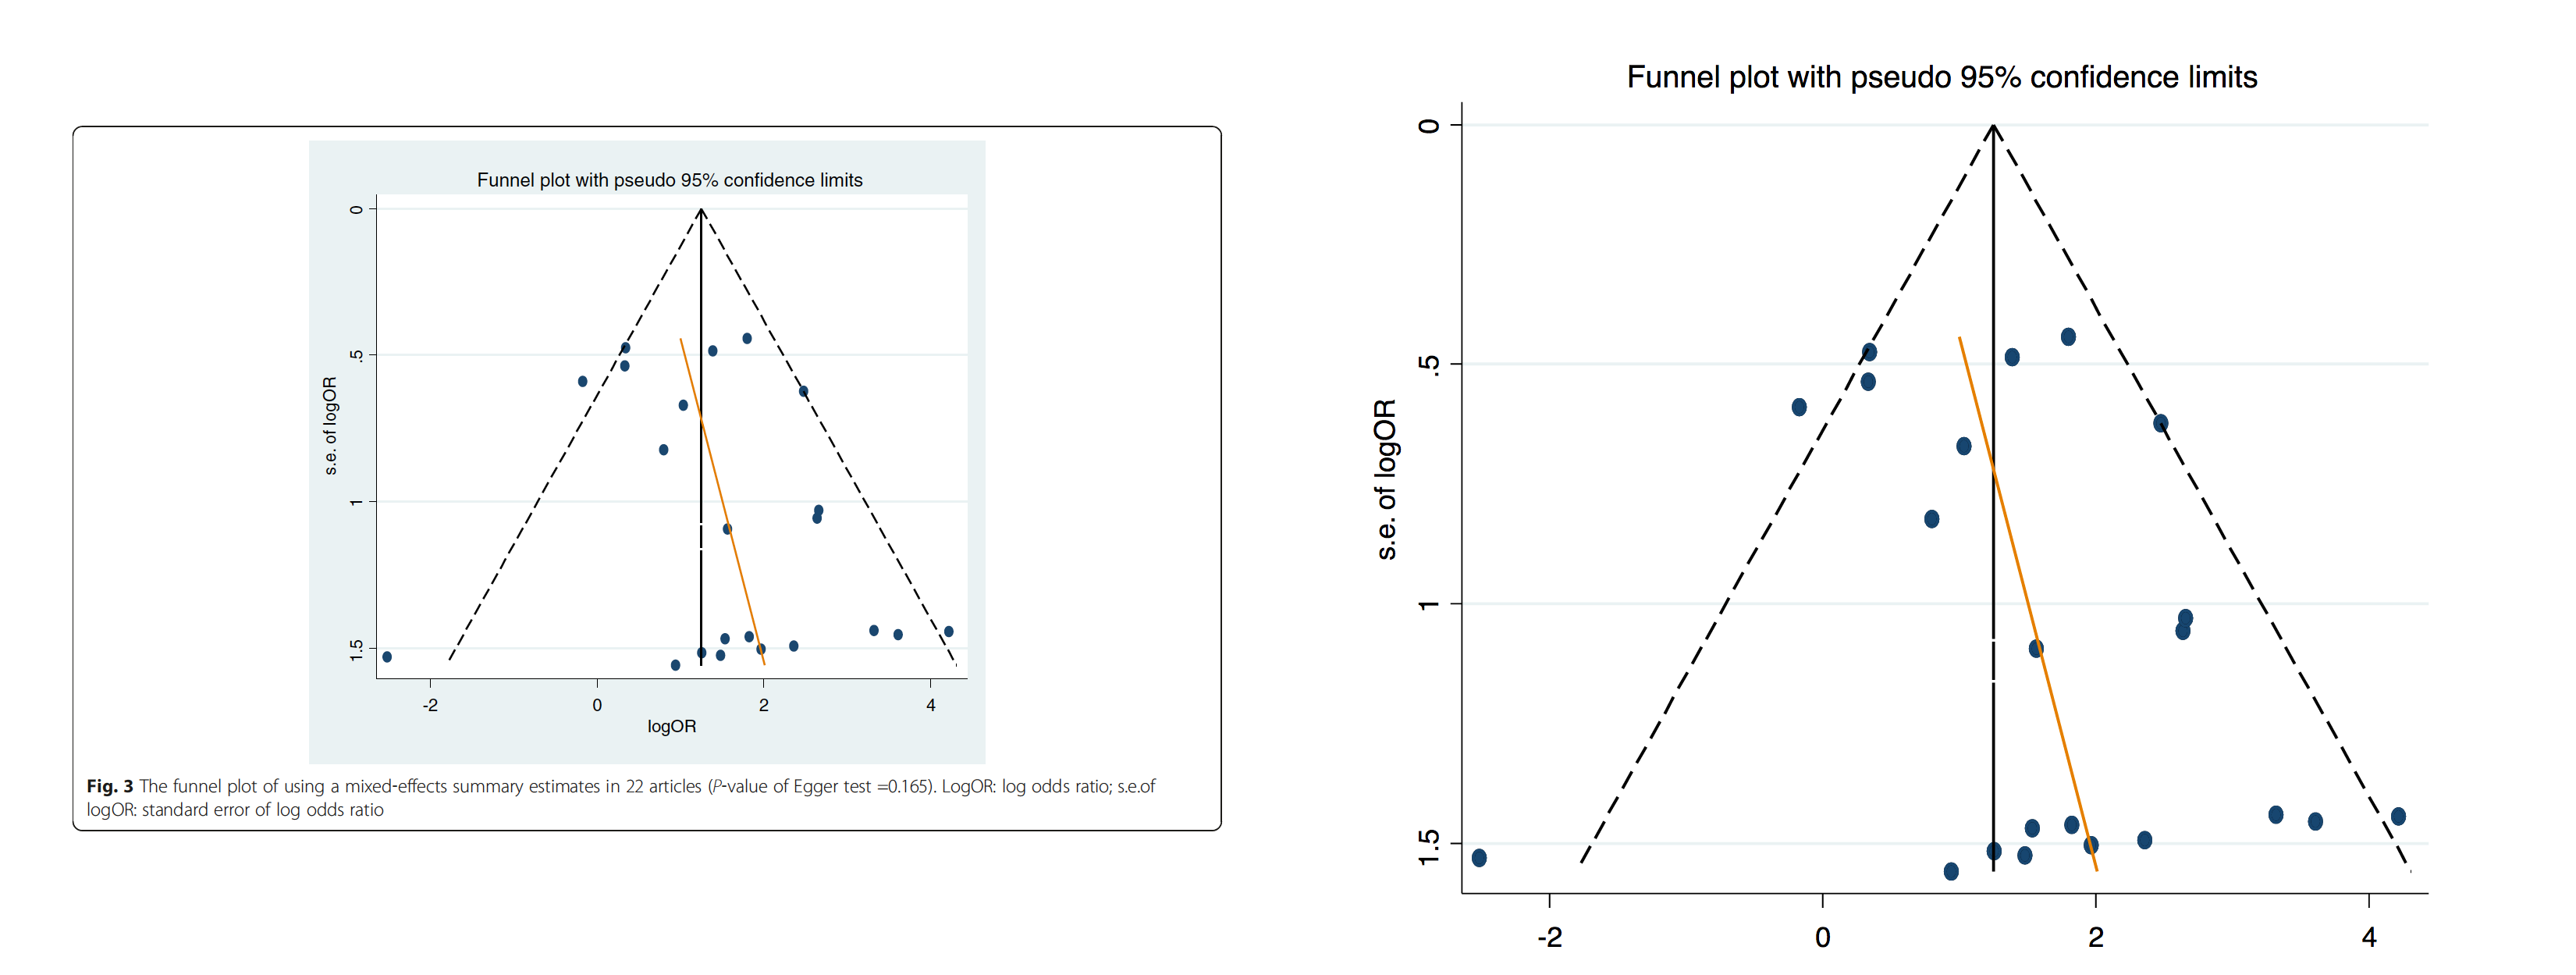
\includegraphics[width=1\linewidth]{assets/figures/boxed-funnel} \caption{The original depiction of a funnel plot [left, reproduced under CC BY license from 10.1186/s13027-016-0058-9] and the manually extracted part that is subsequently ingested into the norma software (right).}\label{fig:vector-fig4}
\end{figure}

Finally, each figure is converted to a data file with \texttt{norma}.
The following command produces an annoted SVG file showing the
identified areas from Figure 1 and a CSV file containing the data based
on the manually clipped figures available in the
\texttt{corpus-clipped/} folder.

\begin{Shaded}
\begin{Highlighting}[]
\ExtensionTok{java}\NormalTok{ -jar bin/norma-0.5.0-SNAPSHOT-jar-with-dependencies.jar \textbackslash{}}
\NormalTok{  --project corpus-clipped \textbackslash{}}
\NormalTok{  --fileFilter }\StringTok{"^.*figures/figure(}\DataTypeTok{\textbackslash{}\textbackslash{}}\StringTok{d+)/figure(_}\DataTypeTok{\textbackslash{}\textbackslash{}}\StringTok{d+)?}\DataTypeTok{\textbackslash{}\textbackslash{}}\StringTok{.svg"}\NormalTok{ \textbackslash{}}
\NormalTok{  --outputDir corpus-clipped \textbackslash{}}
\NormalTok{  --transform scatter2csv}
\end{Highlighting}
\end{Shaded}

We provide the fully extracted data in the folder
\texttt{corpus-extracted/} of the Github repository
(\url{https://github.com/chartgerink/2015ori-3/archive/master.zip}).

\section{Results}\label{results-5}

By searching ScienceOpen, we identified 15 meta-analytic reports
containing vector based funnel plots. Upon manual inspection of the 368
initially found meta-analytic reports, 136 (37\%) contained funnel
plots. Of those 136 meta-analytic reports with funnel plots, we
identified 32 reports (24\%) with vector based images, assuming the
heuristic described in the methods section (i.e., selectable tick
marks). Finally, of those 32 reports with selectable tick marks, 15
reports contained a vector based plot body (47\%).

These 15 reports contained 27 vector funnel plots; we extracted data for
24 funnel plots (89\%) using the software. Table \ref{tab:vector-tab1}
depicts the DOIs and the figure numbers for which we extracted or failed
to extract data. For the 3 funnel plots without extracted data, the
notes indicate potential reasons as to why we were unable to extract the
data. This provides indications as to how the software can be developed
further.

\begin{landscape}\begin{table}[t]

\caption{\label{tab:vector-tab1}All meta-analytic reports with vector based funnel plots and the results of automated data extraction. The figure number depicts the funnel plot order for extraction, the paper figure number depicts the original figure number in the paper. 'Data extracted' indicates whether any datafile was generated by the software. 'Nr. extracted data points' indicates the number of rows in the datafile; 'Nr. manual data points' indicates the visually discernable data points in the plot. 'X-axis correct' and 'Y-axis correct' depicts whether the extracted data corresponded to the data points of the funnel plot upon manual inspection.}
\resizebox{\linewidth}{!}{
\begin{tabular}{lrllrrll}
\toprule
DOI & Fig. nr. & Paper fig. nr. & Data extracted & Nr. extracted data points & Nr. manual data points & X-axis correct & Y-axis correct\\
\midrule
\rowcolor{gray!6}  10.1186/s12885-016-2685-3 & 1 & 4 & yes & 24 & 24 & yes & no\\
10.1186/s12889-016-3083-0 & 1 & 3 & yes & 5 & 5 & no & no\\
\rowcolor{gray!6}  10.1186/s12891-016-1231-4 & 1 & 4 & yes & 6 & 6 & yes & no\\
10.1186/s13027-016-0058-9 & 1 & 3 & yes & 24 & 22 & yes & yes\\
\rowcolor{gray!6}  10.1186/s13054-016-1298-1 & 1 & 4 & no & NA & NA & NA & NA\\
\addlinespace
10.1186/s40064-016-3064-x & 1 & 6a & no & NA & NA & NA & NA\\
\rowcolor{gray!6}  10.1186/s40064-016-3064-x & 2 & 6b & yes & 21 & 8 & no & no\\
10.1186/s40064-016-3064-x & 3 & 6c & yes & 19 & 6 & no & no\\
\rowcolor{gray!6}  10.1515/med-2016-0052 & 1 & 2 & yes & 23 & 23 & yes & yes\\
10.1515/med-2016-0052 & 2 & 4 & yes & 23 & 23 & yes & yes\\
\addlinespace
\rowcolor{gray!6}  10.1515/med-2016-0052 & 3 & 6 & yes & 23 & 23 & yes & yes\\
10.1515/med-2016-0099 & 1 & 7a & yes & 7 & 7 & yes & yes\\
\rowcolor{gray!6}  10.1515/med-2016-0099 & 2 & 7b & yes & 11 & 11 & yes & yes\\
10.1515/med-2016-0099 & 3 & 7c & yes & 10 & 10 & yes & yes\\
\rowcolor{gray!6}  10.1515/med-2016-0099 & 4 & 7d & yes & 7 & 7 & yes & yes\\
\addlinespace
10.1590/S1518-8787.2016050006236 & 1 & 3 & no & NA & NA & NA & NA\\
\rowcolor{gray!6}  10.21053/ceo.2016.9.1.1 & 1 & 3 & yes & 18 & 18 & yes & no\\
10.21053/ceo.2016.9.1.1 & 2 & 3 & yes & 13 & 13 & yes & no\\
\rowcolor{gray!6}  10.21053/ceo.2016.9.1.1 & 3 & 3 & yes & 14 & 14 & yes & yes\\
10.21053/ceo.2016.9.1.1 & 4 & 3 & yes & 9 & 9 & yes & yes\\
\addlinespace
\rowcolor{gray!6}  10.2147/BCTT.S94617 & 1 & 7 & yes & 7 & 7 & no & yes\\
10.3349/ymj.2016.57.5.1260 & 1 & 7 & yes & 24 & 24 & yes & yes\\
\rowcolor{gray!6}  10.3349/ymj.2016.57.5.1260 & 2 & 8 & yes & 12 & 12 & yes & yes\\
10.3390/ijerph13050458 & 1 & 24 & yes & 15 & 15 & yes & no\\
\rowcolor{gray!6}  10.5114/aoms.2016.61916 & 1 & 4 & yes & 5 & 5 & yes & no\\
\addlinespace
10.5114/aoms.2016.61916 & 2 & 4 & yes & 4 & 4 & yes & no\\
\rowcolor{gray!6}  10.5812/ircmj.40061 & 1 & 11 & yes & 30 & 30 & yes & yes\\
\bottomrule
\end{tabular}}
\end{table}
\end{landscape}

Of the 24 funnel plots with extracted data, we correctly extracted data
for 12 funnel plots (50\%). That is, the data points were correctly
mapped onto the x- and y-axis and the number of extracted data points
corresponded to the number of visually discernable data points. For the
remaining 12 funnel plots, there was 1 with correctly mapped x- and
y-axes, but with an incorrect number of extracted data points. For the
remaining 11 funnel plots, the software did not correctly map the axes
or did not extract the correct number of data points.

\section{Discussion}\label{discussion-6}

As the results indicate, vector figures are a fruitful and feasible
resource for data extraction. Based on initial alpha software of
\texttt{norma} to extract data from vector figures, we correctly
extracted data from 50\% of funnel plots for which data was extracted.
This is a very strict assessment, considering our manual investigation
depicted that four extracted datasets (which used a non-standard
direction of the y-axis) only required a simple reversal of one axis to
be 100\% accurate (i.e., 1.23 should be -1.23, etc.), adding a constant
to all data points on an axis to adjust an incorrect mapping, or by
rescaling an axis to fit to the logarithmic scale of one axis. If these
manual corrections for four funnel plots are made, 59\% of all funnel
plots for which data were correctly extracted.

Considering the alpha software to extract data from vectors was
developed in the timespan of approximately one month, we are hopeful
that future development can refine the data extraction and eliminate
some flaws that exist in the alpha software, including those such as
reversed axes, logarithmic axes, etc. The current software was developed
specifically on funnel plots, but its use can be extended to include
other types of plots, such as histograms, etc. Moreover,
third-dimensions such as variable point size provide a fruitful avenue,
considering the SVG also contains information on this (see
\protect\hyperlink{extraction-procedure}{Extraction procedure}).

The main bottleneck for data extraction from vector figures is the
publication of vector figures. In older publications (e.g., scanned
articles) this will be impossible to reconstruct. Our results indicate
that the availability of vector figures in digitally born articles is
relatively sparse; only 15 out of 136 papers with funnel plots contained
vector figures in our sample. From our own anecdotal publishing
experience, vector based figures are often converted into bitmaps in the
editing stage, resulting in loss of information. For publishers
themselves, it is also fruitful to use vector based figures where
possible, considering figure quality is no longer an issue as a result.
As such, we encourage both authors and publishers to produce figures in
vector format (e.g., PDF, SVG, EPS) instead of bitmap format (e.g.,
JPEG, PNG, GIF) when it regards figures presenting results. Not only
will it benefit the quality of the publications, it will also present a
new way of data preservation.

\chapter{As-you-go instead of after-the-fact: A network approach to
scholarly communication and
evaluation}\label{as-you-go-instead-of-after-the-fact-a-network-approach-to-scholarly-communication-and-evaluation}

Scholarly research faces threats to its sustainability and has been said
to face a reproducibility crisis (Baker
\protect\hyperlink{ref-doi:10.1038ux2f533452a}{2016}) amongst other
pernicious problems such as access and exclusivity. The underlying cause
might be the way we have collectively designed the reporting and
rewarding of research (implicitly or explicitly). The current scholarly
communication system is primarily organized around researchers who
publish static (digital) research papers in scholarly journals. Many of
these journals have artificial page limits (in the digital age), which
leads to artificial scarcity and subsequently increases the perceived
prestige of such a journal due to high rejection rates (71\% on average
for APA journals in 2016;
\href{https://perma.cc/Q7AT-RN5C}{perma.cc/Q7AT-RN5C}). Furthermore,
scholarly communication has become highly centralized, where over 50\%
of all papers are published by as little as five publishers (over 70\%
for social sciences; Larivière, Haustein, and Mongeon
\protect\hyperlink{ref-doi:10.1371ux2fjournal.pone.0127502}{2015}).
Centralization has introduced knowledge discrimination, as publishers
are able to influence who can access scholarly knowledge, what gets
published, and allows for other single points of failure to arise with
their own consequences (e.g., censorship;
\href{https://perma.cc/HDX8-DJ8F}{perma.cc/HDX8-DJ8F}). In order to have
a sustainable scholarly research system, we consider it necessary to
implement changes that provide progress on multiple of these threats at
once instead of addressing them individually.

Systems design directly affects what the system and the people who use
it can do; scholarly communication still retains an analog based design
affecting the effectivity of the spread and production of knowledge
dissemination (see also Kling and Callahan
\protect\hyperlink{ref-doi:10.1002ux2faris.1440370105}{2005}).
Researchers and institutions are evaluated on where and how much papers
they publish (as a form of prestige). For example, an oft-used measure
of quality is the Journal Impact Factor (JIF; Garfield
\protect\hyperlink{ref-doi:10.1001ux2fjama.295.1.90}{2006}). The JIF is
also frequently used to evaluate the \enquote{quality} of individual
papers under the assumption that a high impact factor predicts the
success of individual papers, which has been debunked many times
(Prathap, Mini, and Nishy
\protect\hyperlink{ref-doi:10.1007ux2fs11192-016-2034-y}{2016}; Seglen
\protect\hyperlink{ref-Seglen1992}{1992}; Seglen
\protect\hyperlink{ref-Seglen1994}{1994}). Many other performance
indicators in the current system (e.g., citation counts and h-indices)
resort to generic bean counting. Inadequate evaluation measures leave
universities, individual researchers, and funders (amongst others) in
the dark with respect to the substantive questions they might have about
the produced scholarly knowledge. Additionally, work that is not aptly
captured by the authorship of papers is likely to receive less
recognition (e.g., writing software code) due to reward systems counting
publications instead of contributions (see also
\href{https://perma.cc/MUH7-VCA9}{perma.cc/MUH7-VCA9}). It is unfeasible
that a paper-based approach to scholarly communication can escape the
consequences of paper's limitations.

A scholarly communication system is supposed to serve five functions,
but can do so in a narrow sense as it currently does, or in a wider
sense. These functions of the scholarly communication system are (1)
registration-, (2) certification-, (3) awareness-, and (4) archival
(Roosendaal and Geurts \protect\hyperlink{ref-roosendaal1998}{1998}),
and (5) incentives (Sompel et al.
\protect\hyperlink{ref-doi:10.1045ux2fseptember2004-vandesompel}{2004}).
A narrow fulfillment of for example the registration function would mean
that findings that are published are registered, but not all findings
are registered (e.g., due to selective publication; (Franco, Malhotra,
and Simonovits
\protect\hyperlink{ref-doi:10.1126ux2fscience.1255484}{2014})).
Similarly, certification is supposed to occur through peer review, but
peer review can exacerbate human biases in the assessment of quality
(e.g., statistical significance increasing the perceived quality of
methods; Mahoney
\protect\hyperlink{ref-doi:10.1007ux2fbf01173636}{1977}).

We propose an alternative design for scholarly communication based on
modular research outputs with direct links between subsequent modules,
forming a network. Whereas a paper-based approach communicates after a
whole research cycle is completed, modular communication was proposed
two decades ago (Kircz
\protect\hyperlink{ref-doi:10.1108ux2feum0000000007185}{1998}; Sompel et
al.
\protect\hyperlink{ref-doi:10.1045ux2fseptember2004-vandesompel}{2004};
Kuhn et al. \protect\hyperlink{ref-doi:10.7717ux2fpeerj-cs.78}{2016};
Groth, Gibson, and Velterop
\protect\hyperlink{ref-doi:10.3233ux2fisu-2010-0613}{2010}; Velterop
\protect\hyperlink{ref-doi:10.1163ux2f095796511X560006}{2010}; Nielsen
\protect\hyperlink{ref-isbn:9780691148908}{2012}). These modules could
be similar to sections of a research paper, but extend to modular
research outputs such as software or materials. We propose to implement
this modular communication on an \enquote{as-you-go} basis and include
direct links to indicate provenance. This respects the chronological
nature of research cycles and decreases the possibility for pernicious
problems such as selective publication and making predictions after
results are known (HARKing; Kerr
\protect\hyperlink{ref-doi:10.1207ux2fs15327957pspr0203_4}{1998}).

With a network structure between modules of knowledge, we can go beyond
citations and facilitate different questions about single- or
collectives of knowledge. For example, how central is a single module in
the larger network? Or: How densely interconnected is this collective of
knowledge modules? A network could facilitate question-driven evaluation
where an indicator needs to be operationalized per question, instead of
indicators that have become a goal in themselves and become invalidated
by clear cheating behaviors (Seeber et al.
\protect\hyperlink{ref-doi:10.1016ux2fj.respol.2017.12.004}{2017}; ``The
Impact Factor Game''
\protect\hyperlink{ref-doi:10.1371ux2fjournal.pmed.0030291}{2006}). As
such, we propose to make evaluation of research its own research process
with question formulation, operationalizations, and data collection
(i.e., constructing the network of interest).

\section{Network structure}\label{network-structure}

Research outputs are typically research papers, which report on at least
one research cycle after it has occurred. The communicative design of
papers embeds hindsight and its biases in the reporting of results by
being inherently reconstructive. Moreover, this design eliminates the
verification of the chronology within a paper. On the other hand, the
paper encompasses so much that citations to other papers can indicate a
tangent or a crucial link. Additionally, the paper is a bottleneck for
what is communicated: It cannot properly deal with code, data,
materials, etc.

When stages of research are communicated separately and as they occur,
it changes the communicative design to eliminate hindsight and allows
more types of outputs to be communicated as separate modules. For
example, a theory can be communicated first and hypotheses communicated
second, as a direct descendant of the theory. Subsequently, a study
design can be linked as a direct descendant of the hypotheses, materials
as a direct descendant of the design, and so on. This would allow for
the incorporation of materials, data, and analysis code (amongst
others). In this structure, many modules could link to a single module
(e.g., replication causes many data modules to connect to the same
hypotheses module) but one module can also link to many other modules
(e.g., when hypotheses follow from multiple theories or when a
meta-analytic module is linked to many results modules).

Figure \ref{fig:asyougo-fig1} shows two simple examples of how these
different modular research outputs (i.e., modules) would directly
connect to each other. The connection between these modules only shows
the direct descendance and could still include citations to other pieces
of information. For example, a discussion module could be a direct
descendant of a results module and could still include citations to
other relevant findings. When one research cycle ends, a new one can
link to the last module, continuing the chain of descendance.
Incorporating the direct descendancy of these knowledge modules builds a
different kind of network than citation and authorship networks. As
such, this network would be an addition to these already existing
citation and authorship networks; it does not seek to replace them.

\begin{figure}
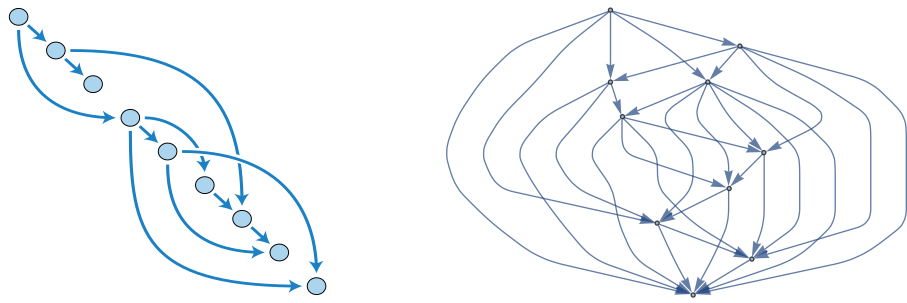
\includegraphics[width=1\linewidth]{assets/figures/Panel with DAGs} \caption{Two Directed Acyclic Graphs (DAGs) of connected research stages. The ordering is chronological (top-bottom) and therefore modules that are situated below one another cannot refer upwards. Panel A shows a less complex network of modules; Panel B shows a more extensive network of modules.}\label{fig:asyougo-fig1}
\end{figure}

Given that these modular outputs would be communicated as they occur,
chronology is directly embedded in the communication process with many
added benefits. For example, preregistration of hypotheses tries to
ensure that predictions precede observations, which would be embedded
with modular communication where predictions are communicated when they
are made (exploratory research could be communicated without hypotheses;
for a more extensive discussion of the benefits and limits of
preregistration see Nosek et al.
\protect\hyperlink{ref-doi:10.1073ux2fpnas.1708274114}{2018}). Moreover,
if modular outputs are communicated as they are produced, selective
reporting (i.e., publication bias) is reduced by having already
communicated the data before results are generated.

With immutable append-only registers, the chronology and content
integrity of these outputs can be ensured and preserved over time. This
can occur efficiently and elegantly with the Dat protocol (without a
blockchain; \href{https://perma.cc/GC8X-VQ4K}{perma.cc/GC8X-VQ4K}). In
short, the Dat protocol is a peer-to-peer protocol (i.e., decentralized
and openly accessible) that provides non-adjustable timestamps to each
change that occurs within a folder, which is given a permanent unique
address on the peer-to-peer Web (\(36^{64}\) addresses possible; Ogden
\protect\hyperlink{ref-doi:10.31219ux2fosf.ioux2fnsv2c}{2017}). The full
details, implications, and potential implementations of this protocol
for scholarly communication fall outside of the scope of this chapter
(an extended technical explanation of the application of the Dat
protocol can be found in the next chapter).

A continuous and network based communication system could take a wider
interpretation of the scholarly functions it is supposed to serve
(Roosendaal and Geurts \protect\hyperlink{ref-roosendaal1998}{1998};
Sompel et al.
\protect\hyperlink{ref-doi:10.1045ux2fseptember2004-vandesompel}{2004}).
Registration would become more complete, because selective publication
based on results is preempted by embedding communication before any
results are known. Certification is improved by embedding the chronology
of a research cycle into the communication of research, ensuring that
predictions precede results (Nosek et al.
\protect\hyperlink{ref-doi:10.1073ux2fpnas.1708274114}{2018}). Awareness
is improved by using open by design principles, whereas awareness is now
limited by financial means to access scholarly papers (Tennant et al.
\protect\hyperlink{ref-doi:10.12688ux2ff1000research.12037.3}{2017}).
Archival would not only be simplified with peer-to-peer protocols, but
also allows anyone to create a copy and could result in excessive
redundancy under the Lots Of Copies Keeps Stuff Safe principle (LOCKSS;
Reich and Rosenthal
\protect\hyperlink{ref-doi:10.1045ux2fjune2001-reich}{2001}). In the
next sections, we extend on how incentives could be adjusted in such a
network structure, to facilitate both the evaluation of research(ers)
and the planning of research.

\section{Indicators}\label{indicators}

With a chronological ordering of various modular research outputs and
their parent relations, a directional adjacency matrix can be extracted
for network analysis. Table \ref{tab:asyougo-tab1} shows the directional
adjacency matrix for Figure \ref{fig:asyougo-fig1} (Panel A). Parent
modules (i.e., modules) must precede the child modules in time,
therefore only \(\frac{J(J-1)}{2}\) of cells of the adjacency matrix are
filled in, where \(J\) is the number of research modules.

\begin{table}[!h]

\caption{\label{tab:asyougo-tab1}Directional adjacency matrix for Figure 1. modules are ordered according to time (top-bottom in Figure 1). Rows indicate the source module, columns indicate the target module.}
\centering
\resizebox{\linewidth}{!}{
\begin{tabular}{llllllllll}
\toprule
 & module01 & module02 & module03 & module04 & module05 & module06 & module07 & module08 & module09\\
\midrule
\rowcolor{gray!6}  module01 &  & 1 & 0 & 1 & 0 & 0 & 0 & 0 & 0\\
module02 &  &  & 1 & 0 & 0 & 0 & 1 & 0 & 0\\
\rowcolor{gray!6}  module03 &  &  &  & 0 & 0 & 0 & 0 & 0 & 0\\
module04 &  &  &  &  & 1 & 1 & 0 & 0 & 1\\
\rowcolor{gray!6}  module05 &  &  &  &  &  & 0 & 0 & 1 & 1\\
\addlinespace
module06 &  &  &  &  &  &  & 1 & 0 & 0\\
\rowcolor{gray!6}  module07 &  &  &  &  &  &  &  & 1 & 0\\
module08 &  &  &  &  &  &  &  &  & 0\\
\rowcolor{gray!6}  module09 &  &  &  &  &  &  &  &  & \\
\bottomrule
\end{tabular}}
\end{table}

With a directional adjacency matrix, countless network indicators can be
calculated that could be useful in research evaluation depending on the
questions asked. However, not all network indicators are directly
applicable because a time based component is included in the network
(i.e., new outputs cannot refer to even newer outputs). Below, we
propose some basic network indicators for evaluating past and future
research outputs.

Networks indicators could be used to evaluate the network as it exists
now or how it developed in the past (i.e., backward-looking evaluation).
For example, in-degree centrality could be used to identify highly
interconnected modules of information. This measure indicates how many
child modules are spawned by a parent module and indicates how much new
work a researcher's output stimulates (e.g., module04 in Table
\ref{tab:asyougo-tab1} would have an in-degree centrality of three). To
contextualize this, a data module could spawn four results modules,
hence has an in-degree centrality of four. This measure would look only
at one-generation of child modules, but other measures extend this to
incorporate multiple generations of child modules. Katz centrality
extends this and computes the centrality over \(N\) generations of child
modules (pp.~206-210; Wasserman and Faust
\protect\hyperlink{ref-isbn:9780521387071}{1994}) whereas traditional
in-degree centrality calculates centrality for \(N=1\) generations. For
example, two data modules that each spawn five results modules would
have the same in-degree centrality, but could have different Katz
centrality if only one of those two networks has a third-generation of
modules included. If multi-generation indicators are relevant, Katz
centrality measures could provide operationalizations of such measures.

Another set of network indicators could be used to evaluate how the
network would change when new modules are added in the future (i.e.,
forward-looking evaluation). For example, a researcher who is looking
for ways to increase the density in their own network, could ask the
question \enquote{If I would add one module that has \(k\) parents,
which addition would increase the density the most?} Subsequently, the
researcher could inspect the identified connections for inspiration and
feasibility. Complexity of the new module could be increased by
increasing the number of parent modules to connect (\(k\) in the
question; e.g., five instead of two). Potentially, this could facilitate
creative thinking, where \(k\) is gradually increased over time to
increase the complexity of the issue from a network perspective.

The indicators we highlighted here are simple proposals. Other
indicators from network analysis and graph theory could be applied to
the study of knowledge development when a network structure is available
and we hope to see suggestions to answer questions about the network.
These kinds of analyses are already done within citation networks (e.g.,
Fortunato et al.
\protect\hyperlink{ref-doi:10.1126ux2fscience.aao0185}{2018}) and
authorship networks (e.g., Morel et al.
\protect\hyperlink{ref-doi:10.1371ux2fjournal.pntd.0000501}{2009}), but
we cannot do so with the provenance or planning of knowledge generation
in the current scholarly communication system.

\section{Use cases}\label{use-cases}

We describe three use cases of network based evaluation to contextualize
the ideas proposed above. For each use case, we first provide a general
and non-exhaustive overview of the possibilities with network based
evaluation. Subsequently, we specify a scenario for that use case, how
an evaluation question flows from that scenario, how an indicator to
answer that question could be operationalized, and how that indicator
could inform the evaluation process. With these use cases we hope to
illustrate that network based evaluation could align better with the
implicit evaluation criteria already present in common research
evaluation scenarios.

\subsection{Funders}\label{funders}

Funders of scholarly research often have specific aims when distributing
their financial resources amongst researchers. Funders often use generic
\enquote{one size fits all} indicators to evaluate the quality of
researchers and research (e.g., JIF, h-index, citation counts). Given
that funding calls often have specific aims, these funding calls could
be used as the basis of research evaluation if we move beyond these
generic measures.

A scenario could exist where a funding agency wants to fund researchers
to extend an existing and interconnected research line. This is not an
implausible scenario, where funding agencies aim to fund several million
dollars (or similar in other currencies) in order to increase follow
through in research lines. A specific example might be the Dutch
national funding agency \enquote{Vici} funding scheme, which aims to
fund \enquote{senior researchers who have successfully demonstrated the
ability to develop their own innovative lines of research}
(\url{https://perma.cc/GB83-RE4J}).

Whether researchers who submitted proposals actually built a connected
research line could be evaluated by looking at how interconnected each
researcher's personal network of modules is. Let us assume that a
research line here would mean that new research efforts interconnect
with previous efforts by that same researcher (i.e., building on
previous work). Additionally, we could assume that building a research
line means that the research line becomes more present in the network
over the years. Building a research line thus could be reformulated into
questions about the network of directly linked output and its
development over time.

Operationalizing the concept \enquote{research line} as increased
interconnectedness of modules over time, we could compute the network
density per year. One way of computing density would be to tally the
number of links and divide them by the number of possible links. By
taking snapshots of the network of outputs of that researcher in for
example the last five years on January 1st, we could compute an
indicator to inform us about the development of the researcher's network
of outputs.

The development of network density over time could help inform the
evaluation, but one measure could hardly be deemed the only decision
criterion. As such, it only provides an indication as to whether an
applicant aligns with the aim of the funding agency. Other questions
would still need to be answered by the evaluation committee. For
example, is the project feasible or does the proposal extend the
previous research line? Some of these other questions could also be seen
as questions about the future development of the network and serve as
their own questions to investigate the applicant on.

\subsection{Universities}\label{universities}

Universities can use research evaluation for the internal allocation of
resources and to hire new scientists. As such, a research group within a
university could apply network analysis to assess how (dis)connected a
group's modules are or how their group compares to similar groups at
other institutions. Using network indicators, it could become possible
to assess whether a job applicant fulfills certain criteria, such as
whether their modules connect to existing modules of a group. If a
university wants to stimulate more diversity in research background,
network analysis could also be used to identify those who are further
removed from the current researchers at the institution. Considering
that universities are often evaluated on the same generic indicators as
individual researchers (e.g., JIF) in the rankings, such new and more
precise evaluation tools might also help specify university goals.

Extending the scenario above, imagine a research group that is looking
to hire an assistant professor with the aim of increasing connectivity
between the group's members. The head of the research group made this
her personal goal in order to facilitate more information exchange and
collaborative potential within the group. By making increasing
connectivity within the group an explicit aim of the hiring process, it
can be incorporated into the evaluation process.

In order to achieve the increased connectivity within the research
group, the head of the research group wants to evaluate applicants
relatively but also with an absolute standard. Relative evaluation could
facilitate applicant selection, but absolute evaluation could facilitate
insight into whether any applicant is sufficient to begin with. In other
words, relative evaluation here asks which is the best applicant,
whereas absolute evaluation asks whether the best applicant is good
enough. These decision criteria could be preregistered in order to
ensure a fair selection process.

Increased connectivity could be computed as a difference measure of the
research group's network density with and without the applicant. In
order to take into account the number of produced modules, the computed
density could take into account the number of modules of an applicant.
Moreover, the head stipulates that the minimum increase in network
density needs to be five percentage points. To evaluate applicants, each
gets a score that is made up of the difference between the current
network density and the network density if they were hired. For example,
baseline connectivity within a group might be 60\%, hence, the network
density has to be at least 65\% for one of the applicants to pass the
evaluation criterium.

If the head of the research group relied purely on the increase in
network density as an indicator without further evaluation, a hire that
decreases morale in the research group could easily be made. For
example, it is reasonable to assume that critics of a research group
often link research outputs in a criticism of their work. If such a
person would apply for a job within that group, the density within the
network might be increased but subsequently result in a more hostile
work climate. Without evaluating the content of the applicant that
increases the network density, it would be difficult to assess whether
they would actually increase information exchange and collaborative
potential instead of stifling it.

\subsection{Individuals}\label{individuals}

Individual researchers could use networks to better understand their
research outputs and plan new research efforts. For example, simply
visualizing a network of outputs could prove a useful tool for
researchers to view relationships between their outputs from a different
perspective. Researchers looking for new research opportunities could
also use network analysis to identify their strengths, by comparing
whether specific sets of outputs are more central than others in a
larger network. For example, a researcher who writes software for their
research might find that their software is more central in a larger
network than their theoretical work, which could indicate a fruitful
specialization.

One scenario where network evaluation tools could be valuable for
individual researchers is resource allocation needs to be optimized. A
researcher might want to revisit previous work and conduct a
replication, but only has funds for one such replication. Imagine a
researcher wants to identify an effect that they previously studied and
which has been central to their new research efforts. Identifying which
effect to replicate is intended by this researcher as a safeguard
mechanism to prevent further investment in new studies, if a fundamental
finding proves to not be replicable.

In this resource allocation scenario, the researcher aims to identify
the most central finding in a network. The researcher has conducted many
studies throughout their career and does not want to identify the most
central finding in the entire network of outputs over the years, but
only of the most recent domain they've been working in. As such, the
researcher takes the latest output and traces all the preceding outputs
automatically to five generations, to create a subset of the full
network and to incorporate potential work not done by themselves.

Subsequently, by computing the Katz centrality of the resulting
subnetwork, the researcher can compute the number of outputs generated
by a finding and how many outputs those outputs generated in return. By
assigning this value to each module in the network, the researcher can
identify the most central modules. However, these modules need to be
investigated subsequently in order to see whether they are findings or
something else (e.g., theory; we assume an agnostic infrastructure that
does not classify modules).

Katz centrality can be a useful measure to identify which finding to
replicate in a multi-generational network, but would fail to take into
account what replications have already been conducted. When taking the
most recent output and looking at its parent(s), grandparent(s), etc.,
this only looks at the lineage of the finding. However, the children of
all these parents are not taken into account in such a trace. As such,
the researcher in our scenario might identify an important piece of
research to replicate, but neglect that it has already been replicated.
Without further inspection of the network for already available
replications, resource allocation might be suboptimal after all.

\section{Discussion}\label{discussion-7}

We propose to communicate research in modular \enquote{as-you-go}
outputs (e.g., theory followed by hypotheses, etc.) instead of large
\enquote{after-the-fact} papers. Modular communication opens up the
possibility of a network of knowledge to come into existence when these
pieces are linked (e.g., results descend from data). This network of
knowledge would be supplementary to traditional citation networks and
could facilitate new evaluation tools that are based in the question of
interest rather than generic \enquote{one size fits all} indicators
(e.g., Journal Impact Factor, citation counts, number of publications).
Given the countless questions and operationalizations possible to
evaluate research in a network of knowledge, we hope this would increase
the focus on indicators as a tool in the evaluation process instead of
indicators being the evaluation process itself (Hicks et al.
\protect\hyperlink{ref-doi:10.1038ux2f520429a}{2015}; Wilsdon et al.
\protect\hyperlink{ref-doi:10.13140ux2fRG.2.1.4929.1363}{2015}).

We highlighted a few use cases and potential indicators for funders,
research collectives, and individuals, but recognize that we are merely
scratching the surface of possible use cases and implementations of
network analysis in research evaluation. The use cases presented for the
various target groups (e.g., universities) can readily be transferred to
suit other target groups (e.g., individuals). Award committees might use
critical path analysis or network stability analysis to identify key
hubs in a network to recognize. Moreover, services could be built to
harness the information available in a network to identify people who
could be approached for collaborations or to facilitate the ease with
which such network analyses can be conducted. Future work could
investigate more use cases, qualitatively identify what researchers (or
others) would like to know from such networks, and how existing network
analysis methods could be harnessed to evaluate research and better
understand its development over time. Despite our enthusiasm for network
based evaluation, we also recognize the need for exploring the potential
negative sides of this approach. Proximity effects might increase bias
towards people already embedded in a network and might exacerbate
inequalities already present. Researchers might also find ways to game
these indicators, which warrants further investigation.

Communicating scholarly research in modular \enquote{as-you-go} outputs
might also address other threats to research sustainability. In modular
\enquote{as-you-go} communication, selective publication based on
results would be reduced because data would be communicated before
results are known. Similarly, adjusting predictions after results are
known would be reduced because predictions would be communicated before
data are available (i.e., preregistration by design). Replications (or
reanalyses) would be encouraged both for the replicated (the replicated
module gets more child modules, increasing its centrality) and the
replicator (time investment is lower due to only having to add a data
module that is linked to the materials module of the replicated).
Self-plagiarism could be reduced by not forcing researchers to rehash
the same theory across papers that spawn various predictions and
studies. These various issues (amongst other out of scope issues) could
be addressed jointly instead of each issue vying for importance for
researchers, funders, or policy makers (amongst others).

To encourage culture- and behavioral change, \enquote{after-the-fact}
papers and modular \enquote{as-you-go} outputs could co-exist
(initially) and would not require researchers to make a zero-sum
decision. Copyright is often transferred to publishers upon publication
(resulting in pay-to-access), but only after a legal contract is signed.
Hence, preprints cannot legally be restricted by publishers when they
precede a copyright transfer agreement. However, preprints face
institutional and social opposition (Kaiser
\protect\hyperlink{ref-doi:10.1126ux2fscience.aaq0747}{2017}), where
preprinting could exclude a manuscript for publication depending on
editorial policies or due to fears of non-publication or scooping
(itself a result of hypercompetition). In recent years, preprints have
become more widely accepted and less likely to exclude manuscript
publication (e.g., Science accepts preprinted manuscripts; Berg
\protect\hyperlink{ref-doi:10.1126ux2fscience.aaq0167}{2017}).
Similarly, sharing modular \enquote{as-you-go} outputs could not legally
be restricted by publishers and can ride the wave of preprint
acceptance, but might also face institutional or social counterchange
similar to preprints. Researchers could communicate \enquote{as-they-go}
and compile \enquote{after-the-fact} papers, facilitating co-existence
and minimizing negative effects on career opportunities. Additionally,
\enquote{as-you-go} modules could be used in any scholarly field where
the provenance of information is important to findings and is not
restricted to empirical and hypothesis driven research per se.

As far as we know, modular \enquote{as-you-go} scholarly communication
infrastructure that includes direct links between modules has not yet
been available to researchers in a sustainable way. One of the few
thought styles that has facilitated \enquote{as-you-go} reporting in the
past decade is that of Open Notebook Science (ONS; Bradley
\protect\hyperlink{ref-doi:10.1038ux2fnpre.2007.39.1}{2007}), where
researchers share their day-to-day notes and thoughts. However, ONS has
remained on the fringes of the Open Science thought style and has not
matured, limiting its usefulness and uptake. For example, ONS increases
user control because communication occurs on personal domains, but does
not have a mechanism of preserving the content. Considering reference
rot occurs in seven out of ten scholarly papers containing Weblinks (M.
Klein et al.
\protect\hyperlink{ref-doi:10.1371ux2fjournal.pone.0115253}{2014}),
concern for sustainable ONS is warranted without further development of
content integrity. Moreover, ONS increases information output without
providing more possibilities of discovering that content.

Digital infrastructure that facilitates \enquote{as-you-go} scholarly
communication is now feasible and sustainable. Feasible because the
peer-to-peer protocol Dat provides stable addresses for versioned
content and it ensures content integrity across those versions.
Sustainable because preservation in a peer-to-peer network is relatively
trivial (inherent redundancy, anyone can rehost information and
libraries could be persistent hosters) and removes (or at least reduces)
the need for centralized services in scholarly communication.
Consequently, this decreases the need for inefficient server farms of
centralized services (Cavdar and Alagoz
\protect\hyperlink{ref-doi:10.1109ux2fglocom.2012.6503613}{2012}) by
decentralizing services. However, preservation is a social process that
requires commitment. Hence, a peer-to-peer infrastructure would require
committed and persistent peers (e.g., libraries) to make sure content is
preserved. Another form of sustainability is knowledge inclusion, which
is facilitated by a decentralized network protocol that is openly
accessible.

Finally, we would like to note that communication was not instantly
revolutionized by the printing press but changed society over the
centuries that followed. The Web has only been around since 1991 and its
effect on society is already pervasive, but far from over. We hope that
individuals who want change do not despair by feelings of inertia in
scholarly communication throughout recent years and further entrenching
of positions and interests. We remain optimistic for substantial change
to occur within scholarly communication that improves the way we
communicate research and hope these ideas contribute in working towards
that.

\section{Conclusion}\label{conclusion-1}

The current scholarly communication system based on research papers is
\enquote{after-the-fact} and can be supplemented by a modular
\enquote{as-you-go} based communication system. By doing so, the
functions of a scholarly communication system can be interpreted more
widely, making registration complete, certification part of the process
instead of just the judgment of peers, access to everything for everyone
based on peer-to-peer protocols, simplify archival, and facilitate
incentive structures that could align researcher's interests with that
of scholarly research.

\chapter{Verified, shared, modular, and provenance based research
communication with the Dat
protocol}\label{verified-shared-modular-and-provenance-based-research-communication-with-the-dat-protocol}

In scholarly research, communication needs to be thorough and
parsimonious in logging the order of various research steps, while at
the same time being functional in seeking- and distributing knowledge.
Roosendaal and Geurts proposed that any scholarly communication system
needs to serve as a (1) registration-, (2) certification-, (3)
awareness-, and (4) archival system (Roosendaal and Geurts
\protect\hyperlink{ref-roosendaal1998}{1998}). Sompel and colleagues
added that it also needs to serve as an (5) incentive system (Sompel et
al.
\protect\hyperlink{ref-doi:10.1045ux2fseptember2004-vandesompel}{2004}).

How the functions of scholarly communication are conceptualized and
implemented directly impacts (the effectiveness of) scholarly research.
For example, an incentive system might be present where number of
publications or publication outlet is more important than the quality of
the publications (Brembs
\protect\hyperlink{ref-doi:10.3389ux2ffnhum.2018.00037}{2018}). In a
narrow sense, this scholarly communication system serves the fifth
function of providing an incentive system. In a wider sense, it
undermines the goal of scholarly research, which scholarly communication
is a part of, and therefore does not serve its purpose.

Narrow conceptualizations of the functions of a scholarly communication
system can be identified throughout the current article-based system.
Registration occurs for published works, but registration is incomplete
due to selective publication (e.g., 1 out of 2 registered clinical
trials gets published; Easterbrook et al.
\protect\hyperlink{ref-doi:10.1016ux2f0140-6736_91_90201-y}{1991})
making research highly inefficient (Van Assen et al.
\protect\hyperlink{ref-doi:10.1371ux2fjournal.pone.0084896}{2014}).
Certification occurs through peer review (Sompel
\protect\hyperlink{ref-doi:10.1038ux2fnature05008}{2006}) but peer
review is confounded by a set of human biases at the reporting- and
evaluation stages (e.g., methods are evaluated as of higher quality when
they result in statistically significant results than when in
statistically nonsignificant results; Mahoney
\protect\hyperlink{ref-doi:10.1007ux2fbf01173636}{1977}), leading to the
\enquote{natural selection of bad science} (Smaldino and McElreath
\protect\hyperlink{ref-doi:10.1098ux2frsos.160384}{2016}). Awareness
occurs, but increasingly only for those researchers with the financial
means to access or make accessible (Khoo
\protect\hyperlink{ref-doi:10.18352ux2flq.10280}{2019}). Restrictions on
the sharing of scholarly information hampers discovery and widespread
dissemination. Content is archived, but is centralized (i.e., failure
prone), separated from the main dissemination infrastructure, and not
available until an arbitrary trigger event occurs (i.e., a dark archive;
Kiefer \protect\hyperlink{ref-doi:10.1629ux2fuksg.215}{2015}).

The scholarly paper seems an anachronistic form of communication in
light of how we now know it undermines the functions it is supposed to
serve. When no alternative communication form was feasible (i.e., before
the Internet and the Web), the scholarly paper seemed a reasonable and
balanced form for communication. However, already in 1998, seven years
after the first Web browser was released, researchers associated with
the scholarly publisher Elsevier suggested to make changes to the way
scholars communicate scholarly research (Kircz
\protect\hyperlink{ref-doi:10.1108ux2feum0000000007185}{1998}). More
specifically, they suggested to change the communication to a more
modular form, which would help iterate research more frequently and
increase feedback moments (high speed of feedback was essential to for
example Nature's rise during the early twentieth century; Baldwin
\protect\hyperlink{ref-isbn:9780226261454}{2015}). Throughout the years,
others also suggested various perspectives on modularity (Priem and
Hemminger \protect\hyperlink{ref-doi:10.3389ux2ffncom.2012.00019}{2012};
Kuhn et al. \protect\hyperlink{ref-doi:10.7717ux2fpeerj-cs.78}{2016})
and suggested micro- and nanopublications (Kuhn et al.
\protect\hyperlink{ref-doi:10.7717ux2fpeerj-cs.78}{2016}; Clark,
Ciccarese, and Goble
\protect\hyperlink{ref-doi:10.1186ux2f2041-1480-5-28}{2014}). One
example of modular, stepwise research communication is depicted in
Figure \ref{fig:octopi}.

\begin{figure}[h]
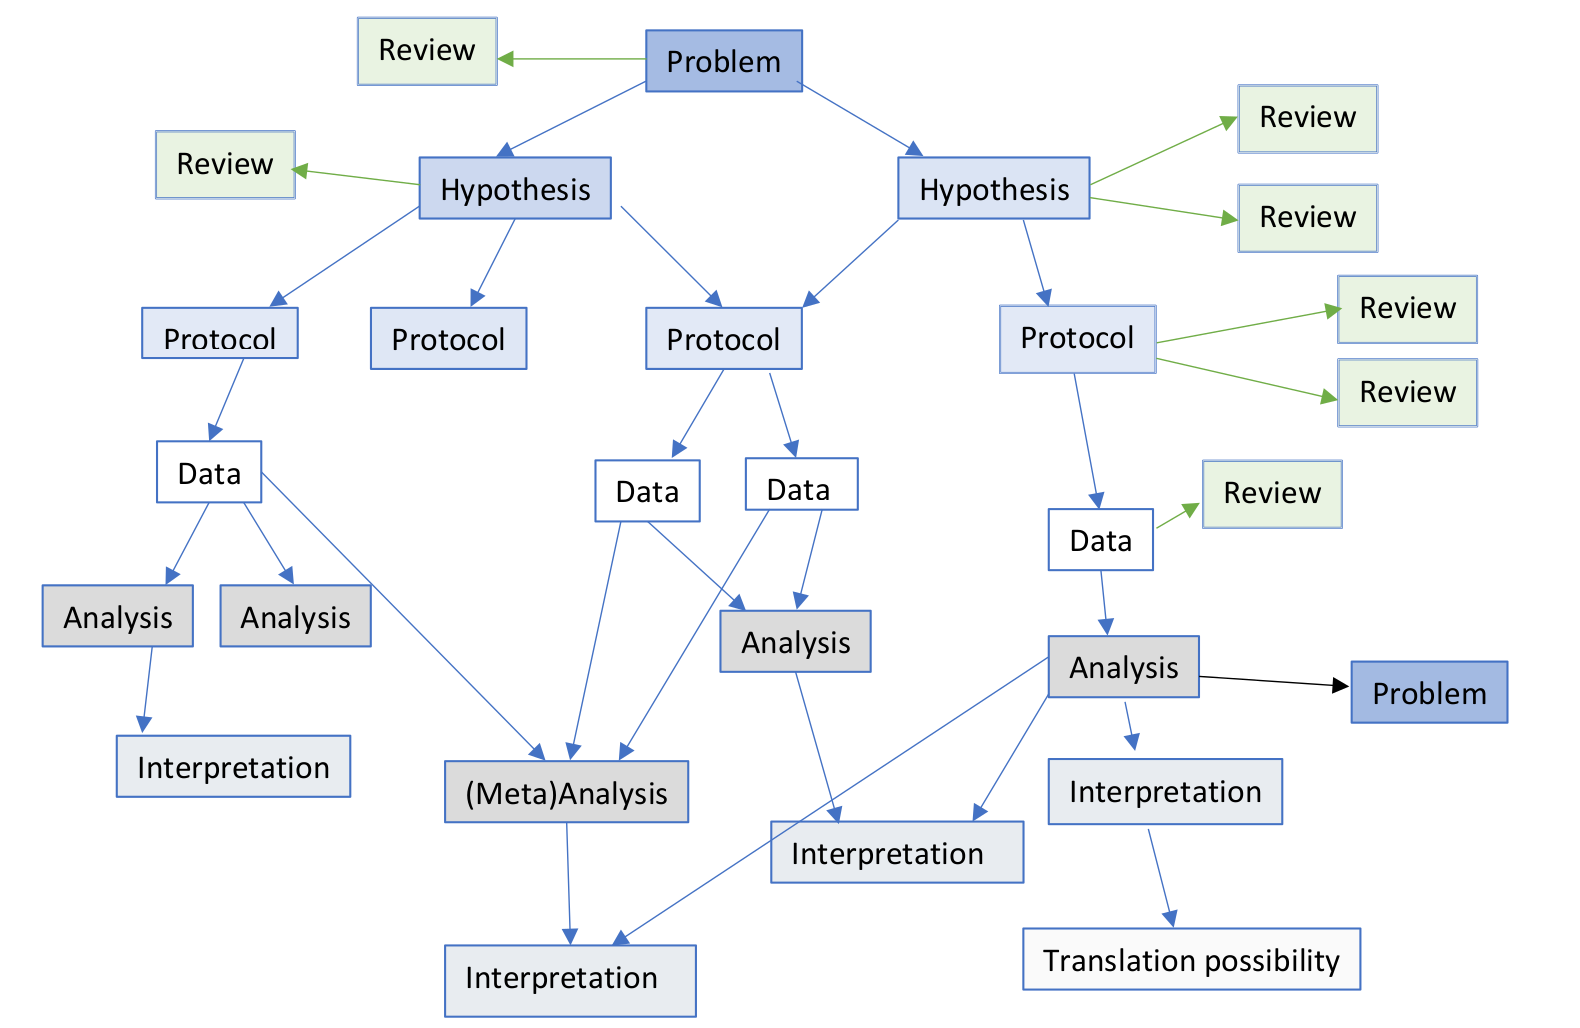
\includegraphics[width=1\linewidth]{assets/figures/fig-octo} \caption{An example of modular, stepwise research communication, from the Octopus project (see also https://perma.cc/TA79-YPH9).}\label{fig:octopi}
\end{figure}

Modular scholarly outputs, each a separate step in the research process,
could supplement the scholarly article (as detailed in Hartgerink and
Zelst \protect\hyperlink{ref-doi:10.3390ux2fpublications6020021}{2018}).
Scholarly textbooks and monographs (i.e., vademecum science; Fleck
\protect\hyperlink{ref-isbn:9780226253251}{1984}) communicate findings
with few details and a high degree of certainty; scholarly articles
present relatively more details and less certainty than textbooks, but
still lack the detail to reproduce results. This lack of detail is
multiplied by the increasingly complex research pipelines due to
technological changes and the size of data processed. Moreover,
textbooks and articles construct narratives across findings because they
report far after events have happened and it is what editors expect.
Scholarly modules could serve as the base for scholarly articles,
reporting more details, less certainty of findings, and where events are
reported closer to their occurrence. Granular reporting may help
facilitate a shift from authorship to contributorship (Holcombe
\protect\hyperlink{ref-doi:10.31234ux2fosf.ioux2fdt6e8}{2019}), could
facilitate reproducibility (i.e., it is easier to reproduce one action
with more details than multiple actions with fewer details per action);
earlier reporting could facilitate discussion by making it practical for
the research process (extending the idea of Registered Reports; Chambers
\protect\hyperlink{ref-doi:10.1016ux2fj.cortex.2012.12.016}{2013}) and
making content easier to find and reuse. As findings become replicated
and more consensus about a finding starts to arise, findings could move
up the \enquote{chain} and be integrated into scholarly articles and
textbooks. Articles and books would then provide overviews and larger
narratives to understand historical developments within scholarly
research. Figure \ref{fig:datcom-fig1} provides a conceptual depiction
of how these different forms of documenting findings relate to each
other.

\begin{figure}[h]

{\centering 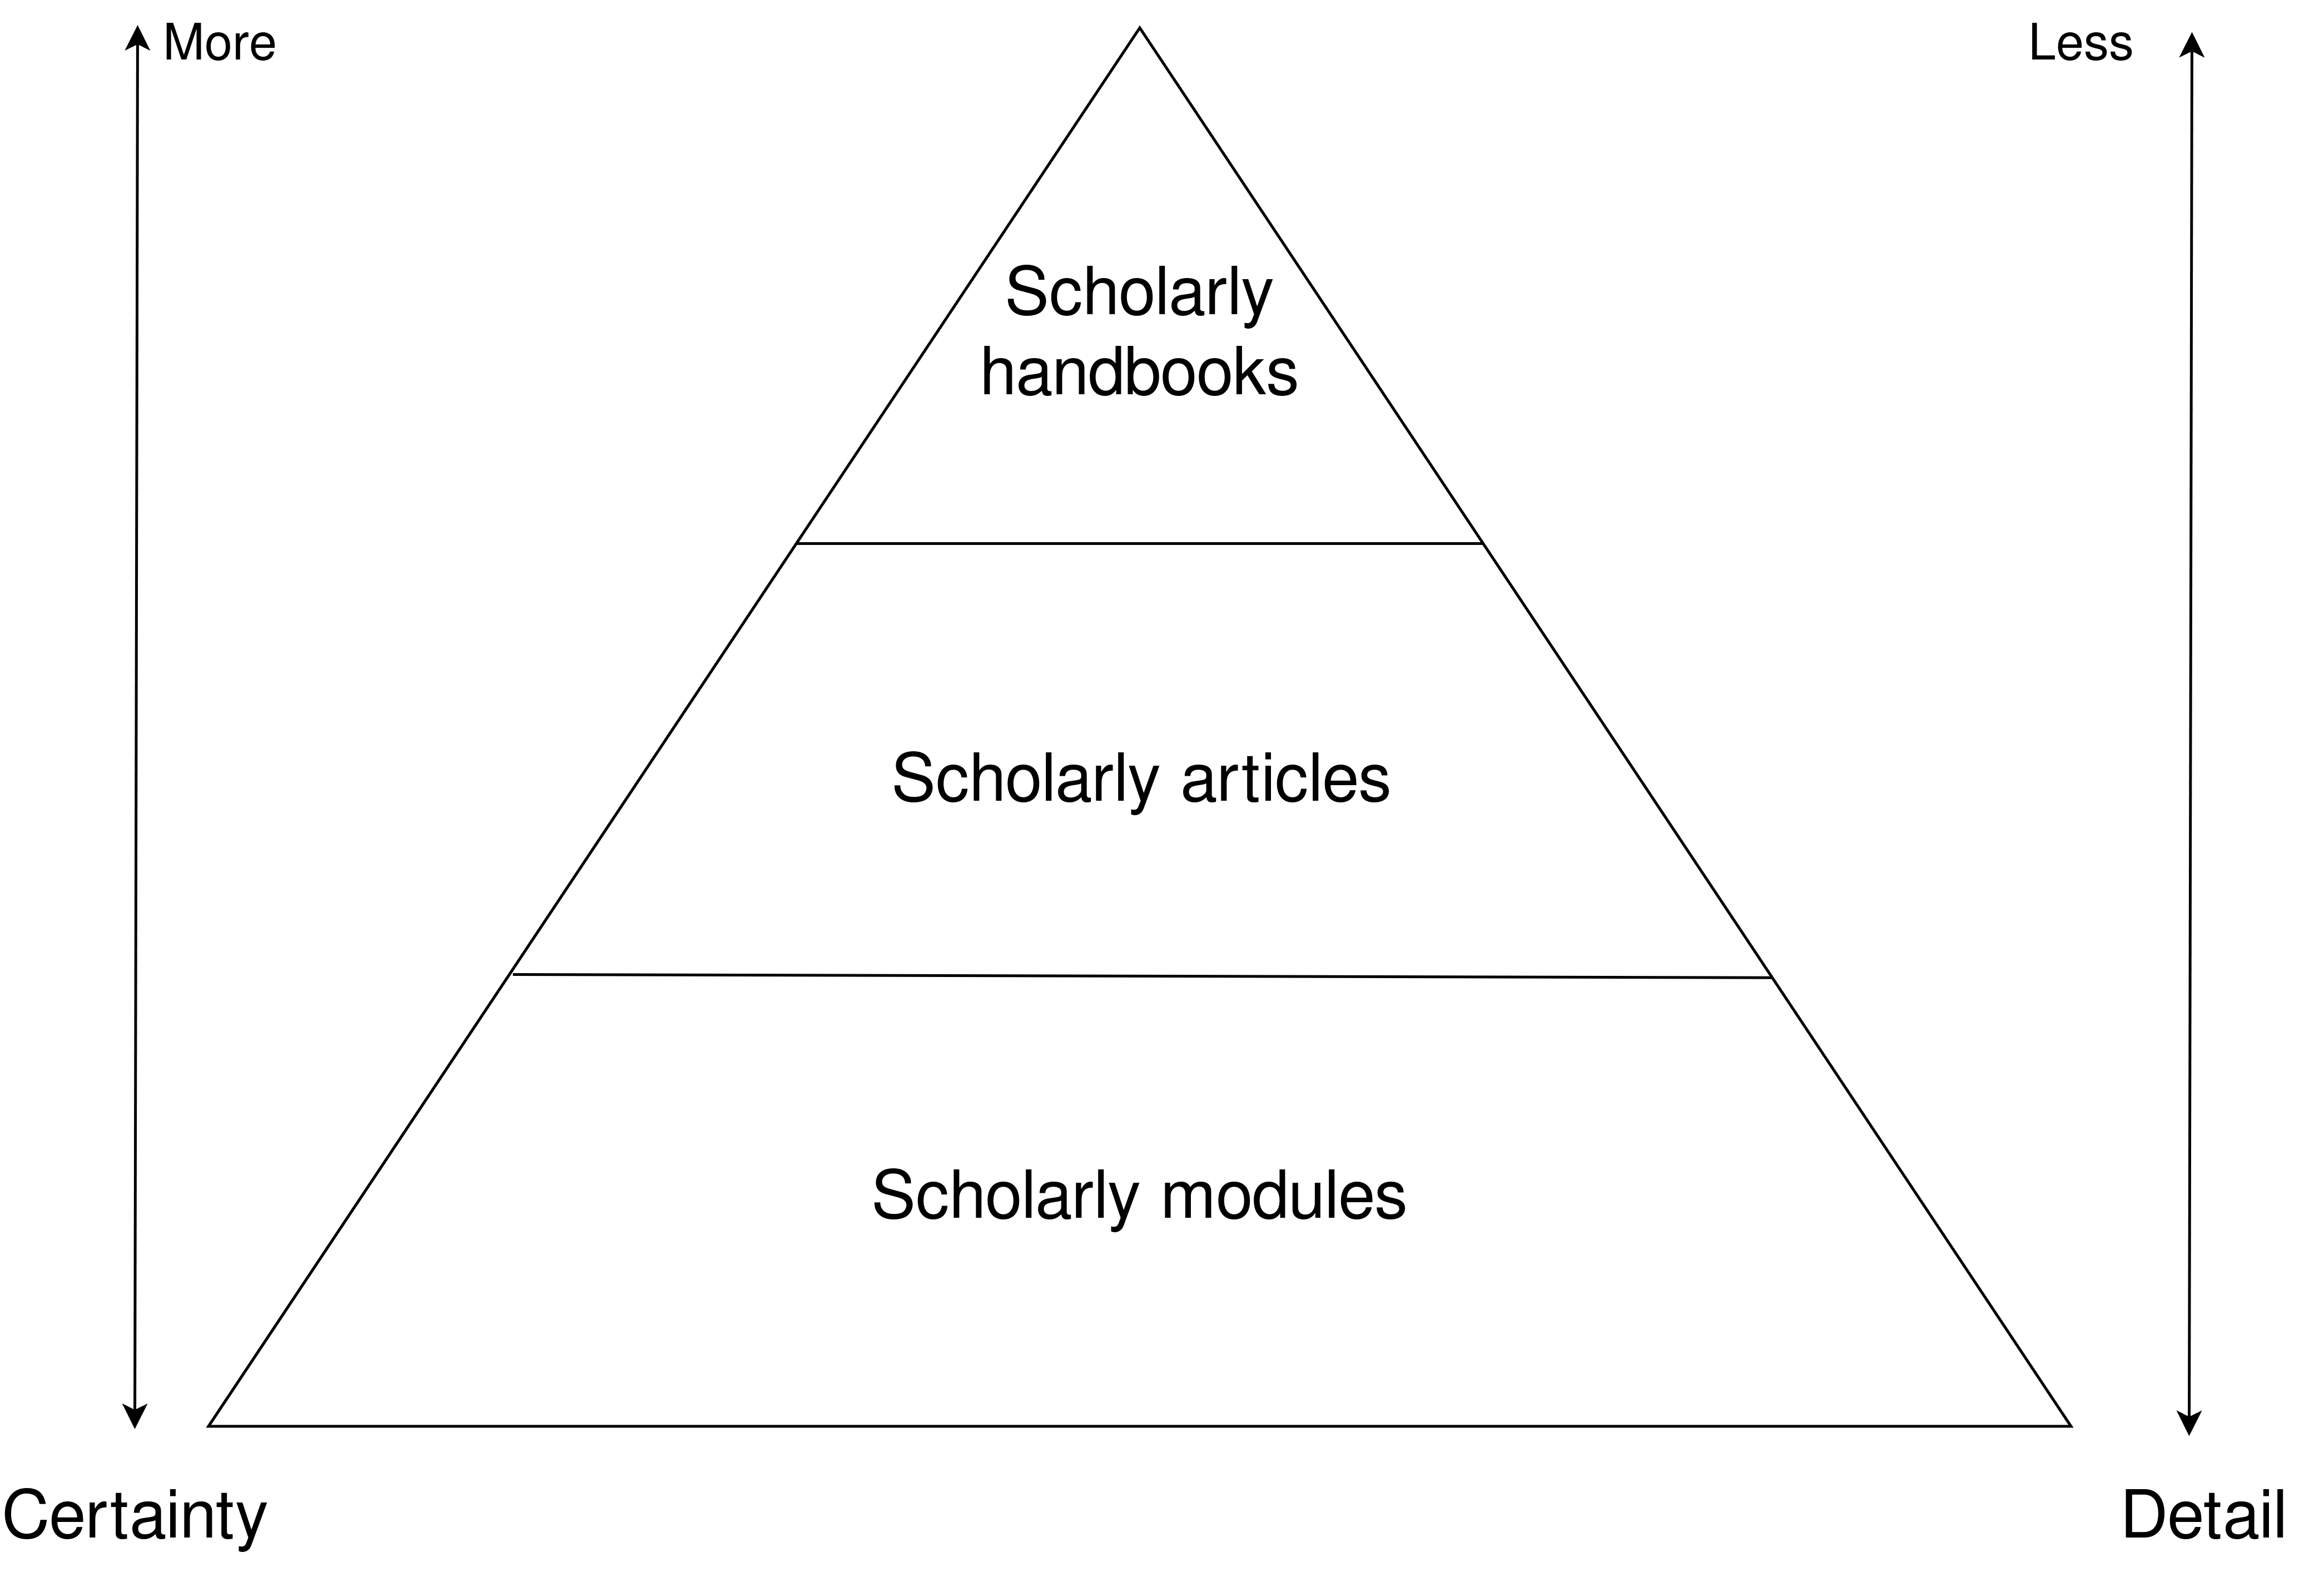
\includegraphics[width=0.8\linewidth]{assets/figures/datcom-fig1} 

}

\caption{Conceptual depiction of how different forms of scholarly communication relate to each other in both detail and certainty.}\label{fig:datcom-fig1}
\end{figure}

Below I extend on technical details for a modular scholarly
communication infrastructure that facilitates (more) continuous
communication and builds on recent advances in Web infrastructures. The
premise of this scholarly infrastructure is a wider interpretation of
the five functions of a scholarly communication system, where (1)
registration is (more) complete, (2) certification by peer review is
supplemented by embedding chronology to prevent misrepresentation and by
increased potential for verification and peer discussion, (3)
unrestricted awareness (i.e., access) is embedded in the underlying
peer-to-peer protocol that locks it open-by-design, (4) archival is
facilitated by simplified copying, and (5) making more specific
scholarly evaluation possible to improve incentives (for an initial
proposal of such evaluation systems see Hartgerink and Zelst
\protect\hyperlink{ref-doi:10.3390ux2fpublications6020021}{2018}).
First, I expand on the functionality of the Internet protocol
\href{https://datproject.org}{Dat} and how it facilitates improved
dissemination and archival. Second, I illustrate an initial design of
modular scholarly communication using this protocol to facilitate better
registration and certification.

\section{Dat protocol}\label{dat-protocol}

The Dat protocol (\texttt{dat://}) is a peer-to-peer protocol, with
persistent public keys per filesystem (see also
\url{https://perma.cc/FX7M-H85Y}; Ogden
\protect\hyperlink{ref-doi:10.31219ux2fosf.ioux2fnsv2c}{2017}; Robinson
et al. \protect\hyperlink{ref-doi:10.1038ux2fsdata.2018.221}{2018}).
Each filesystem is a folder that lives on the Dat network. Upon
creation, each Dat filesystem receives a unique 64 character hash
address, which provides read-only access to anyone who has knowledge of
the hash. Below an example filesystem is presented. Each Dat filesystem
has a persistent public key, which is unaffected by bit-level changes
within it (e.g., when a file is modified or created). Other peer-to-peer
protocols, such as BitTorrent or the Inter Planetary File System (IPFS),
receive new public keys upon bit-level changes in the filesystem and
require re-sharing those keys after each change (at the protocol level).

\begin{Shaded}
\begin{Highlighting}[]
\ExtensionTok{0c6...613/}
\KeywordTok{|}\ExtensionTok{---}\NormalTok{ file1}
\KeywordTok{|}\ExtensionTok{---}\NormalTok{ file2}
\KeywordTok{|}\ExtensionTok{---}\NormalTok{ file3}
\KeywordTok{|}\ExtensionTok{---}\NormalTok{ file4}
\end{Highlighting}
\end{Shaded}

Bit-level changes within a Dat filesystem are verified with
cryptographically signed hashes of the changes in a Merkle Tree. In
effect, using a Merkle Tree creates a verified append-only register. In
a Merkle Tree, contents are decomposed into chunks that are subsequently
hashed in a tree (as illustrated in Figure \ref{fig:datcom-fig2}),
adding each new action to the tree at the lowest level. These hashes are
cryptographically signed with the permitted users' private keys. The Dat
protocol regards all actions in its filesystem as \texttt{put} or
\texttt{del} commands to the filesystem, allowing all operations on the
filesystem to be regarded as actions to append to a register (i.e.,
log). For example, if an empty \texttt{file5} was added to the Dat
filesystem presented above, the register would include
\texttt{{[}put{]}~/file5~0~B~(0~blocks)}; if we delete the file, it
would log \texttt{{[}del{]}~/file5}. The complete register for this Dat
filesystem is as follows

\begin{Shaded}
\begin{Highlighting}[]
\ExtensionTok{dat}\NormalTok{://0c6...613}

\ExtensionTok{1}\NormalTok{ [put] /file1 0 B (0 blocks)}
\ExtensionTok{2}\NormalTok{ [put] /file2 0 B (0 blocks)}
\ExtensionTok{3}\NormalTok{ [put] /file3 0 B (0 blocks)}
\ExtensionTok{4}\NormalTok{ [put] /file4 0 B (0 blocks)}
\ExtensionTok{5}\NormalTok{ [put] /file5 0 B (0 blocks)}
\ExtensionTok{6}\NormalTok{ [del] /file5}
\end{Highlighting}
\end{Shaded}

The persistent public key combined with the append-only register,
results in persistent versioned addresses for filesystems that also
ensure content integrity. For example, based on the register presented
above, we see that version 5 includes \texttt{file5} whereas version 6
does not. By appending \texttt{+5} to the public key
(\texttt{dat://0c66...613+5}) we can view the Dat filesystem as it
existed at version 5 and be ensured that the contents we receive are the
exact contents at that version. If the specific Dat filesystem is
available from at least one peer on the network, it means that both
\enquote{link rot} and \enquote{content drift} (M. Klein et al.
\protect\hyperlink{ref-doi:10.1371ux2fjournal.pone.0115253}{2014}; Jones
et al.
\protect\hyperlink{ref-doi:10.1371ux2fjournal.pone.0167475}{2016}) could
become superfluous.

\begin{figure}[h]

{\centering 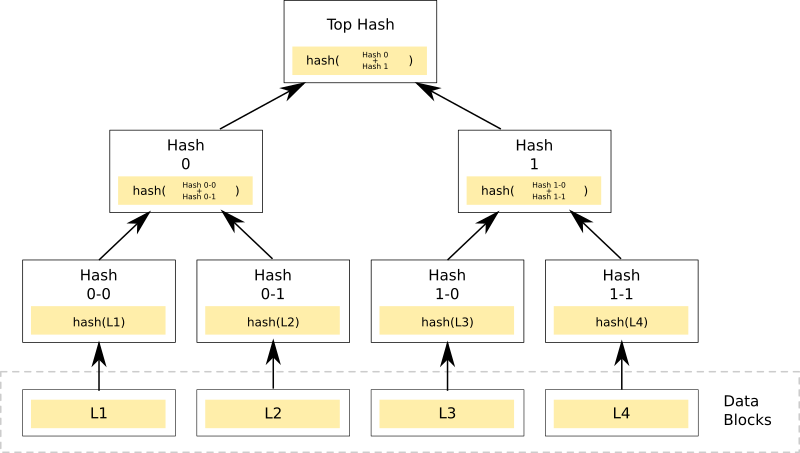
\includegraphics[width=1\linewidth]{assets/figures/datcom-fig2} 

}

\caption{A diagram depicting how a Merkle Tree hashes initial chunks of information into one top hash, with which the content can be verified.}\label{fig:datcom-fig2}
\end{figure}

Any content posted to the Dat protocol is as publicly available as the
public key of that Dat filesystem is shared. More specifically, the Dat
protocol is inherently open. As such, if that key is widely shared, the
content will also be harder or impossible to remove from the network
because other peers (can) have copied it. Conversely, if that key is
shared among just few people that content can more easily disappear from
the network but remains more private. This is important in light of
privacy issues, because researchers cannot unshare personal data after
they have widely broadcasted it. However, because the Dat protocol is a
peer-to-peer protocol and users connect directly to each other,
information is not mediated. The protocol uses package encryption by
default which can also help improve secure and private transfers of
(sensitive) data. Users would (most likely) also remain personally
responsible for the information they (wrongly) disclose on the network.

\section{Verified modular scholarly
communication}\label{verified-modular-scholarly-communication}

Here I propose an initial technical design of verified modular scholarly
communication using the Dat protocol. Scholarly modules are instantiated
as separate Dat filesystems for each researcher or for each module of
scholarly content. Scholarly content could entail virtually anything the
researcher wants or needs to communicate in order to verify findings
(see also Hartgerink and Zelst
\protect\hyperlink{ref-doi:10.3390ux2fpublications6020021}{2018}).
Hence, there is no restriction to text as it is in the current
article-based scholarly communication system; it may also include
photographs, data files, scripts, etc. Note that all presented
hypothetical scenarios next include shortened Dat links and the
unshortened links can be found in the Supporting Information.

\subsection{Scholarly profiles}\label{scholarly-profiles}

Before communicating research modules, a researcher would need to have a
place to broadcast that information. Increasingly, researchers are
acquiring centralized scholarly profiles to identify the work they do,
such as ORCIDs, ResearcherIDs, Google Scholar profiles, or ResearchGate
profiles. A decentralized scholarly profile in a Dat filesystem is
similar and provides a unique ID (i.e., public key) for each researcher.
However, researchers can modify their profiles freely because they
retain full ownership and control of their data (as opposed to
centralized profiles) and are not tied to one platform. As such, with
decentralized scholarly profiles on the Dat network, the researcher
permits others access to their profile instead of a service permitting
them to have a profile.

Each Dat filesystem is initialized with a \texttt{dat.json} with some
initial metadata, including its own Dat public key, the title (i.e.,
name) of the filesystem and a description. For example, Alice wants to
create a scholarly profile and initializes her Dat filesystem, resulting
in:

\begin{Shaded}
\begin{Highlighting}[]
\FunctionTok{\{}
  \DataTypeTok{"title"}\FunctionTok{:} \StringTok{"Alice"}\FunctionTok{,}
  \DataTypeTok{"description"}\FunctionTok{:} \StringTok{"I am a physicist at CERN-LHC. As a fan of the }
\StringTok{    decentralized Web, I look forward to communicating my research}
\StringTok{    in a digital native manner and in a way that is not limited }
\StringTok{    to just text."}\FunctionTok{,}
  \DataTypeTok{"url"}\FunctionTok{:} \StringTok{"dat://b49...551"}
\FunctionTok{\}}
\end{Highlighting}
\end{Shaded}

Because \texttt{dat.json} is a generic container for metadata across the
Dat network, I propose adding \texttt{scholarly-metadata.json} with some
more specific metadata (i.e., data about the profile) for a scholarly
context. As the bare minimum, we initialize a scholarly profile metadata
file as

\begin{Shaded}
\begin{Highlighting}[]
\FunctionTok{\{}
  \DataTypeTok{"type"}\FunctionTok{:} \StringTok{"scholarly-profile"}\FunctionTok{,}
  \DataTypeTok{"url"}\FunctionTok{:} \StringTok{"dat://b49...551"}\FunctionTok{,}
  \DataTypeTok{"parents"}\FunctionTok{:} \OtherTok{[]}\FunctionTok{,}
  \DataTypeTok{"roots"}\FunctionTok{:} \OtherTok{[]}\FunctionTok{,}
  \DataTypeTok{"main"}\FunctionTok{:} \StringTok{"/cv.pdf"}\FunctionTok{,}
  \DataTypeTok{"follows"}\FunctionTok{:} \OtherTok{[]}\FunctionTok{,}
  \DataTypeTok{"modules"}\FunctionTok{:} \OtherTok{[]}
\FunctionTok{\}}
\end{Highlighting}
\end{Shaded}

where the \texttt{type} property indicates it is a scholarly profile.
The \texttt{url} property provides a reference to the public key of
Alice herself (i.e., self-referencing). The \texttt{parents} property is
where Alice can indicate her \enquote{scholarly parents} (e.g.,
supervisors, mentors); the \texttt{roots} property is inherited from her
scholarly parents and links back to the root(s) of her scholarly
genealogy. The \texttt{main} property indicates the main file for
Alice's profile. The \texttt{follows} property links to other
decentralized scholarly profiles or decentralized scholarly modules that
Alice wants to watch for updates. Finally, the \texttt{modules} property
refers to versioned scholarly modules, which serves as Alice's public
registrations. These metadata files may be joined in a later
specification.

Assuming Alice is the first person in her research program to use a
decentralized scholarly profile, she is unable to indicate
\texttt{parents} or inherit \texttt{roots}. However, Bob and Eve are her
PhD students and she helps them set up a decentralized scholarly
profile. As such, their profiles do contain a parent: Alice's profile.
Based on this genealogy, we would be able to automatically construct
self-reported genealogical trees for scholarly profiles. Bob's
\texttt{scholarly-metadata.json} subsequently looks as follows

\begin{Shaded}
\begin{Highlighting}[]
\FunctionTok{\{}
  \DataTypeTok{"type"}\FunctionTok{:} \StringTok{"scholarly-profile"}\FunctionTok{,}
  \DataTypeTok{"url"}\FunctionTok{:} \StringTok{"dat://c3a...a1b"}\FunctionTok{,}
  \DataTypeTok{"parents"}\FunctionTok{:} \OtherTok{[} \StringTok{"dat://b49...551"} \OtherTok{]}\FunctionTok{,}
  \DataTypeTok{"roots"}\FunctionTok{:} \OtherTok{[} \StringTok{"dat://b49...551"} \OtherTok{]}\FunctionTok{,}
  \DataTypeTok{"main"}\FunctionTok{:} \KeywordTok{null}\FunctionTok{,}
  \DataTypeTok{"follows"}\FunctionTok{:} \OtherTok{[]}\FunctionTok{,}
  \DataTypeTok{"modules"}\FunctionTok{:} \OtherTok{[]}
\FunctionTok{\}}
\end{Highlighting}
\end{Shaded}

Alice wants to stay up to date with the work from Bob and Eve and adds
their profiles to the \texttt{follows} property. By adding the unique
Dat links to their scholarly profiles to her \texttt{follows} property,
the profiles can be watched in order to build a chronological feed that
continuously updates. Whenever Bob (or Eve) changes something in their
profile, Alice gets a post in her chronological feed. For example, when
Bob follows someone, when Eve posts a new scholarly module, or when Bob
updates his \texttt{main} property. In contrast to existing social
media, Alice can either fully unfollow Bob, which removes all of Bob's
updates from her feed, or \enquote{freeze follow} where she simply does
not get any future updates. A \enquote{freeze follow} follows a static
and specific version of the profile by adding a version number to the
followed link (e.g., \texttt{dat://...+12}).

\begin{figure}[h]

{\centering 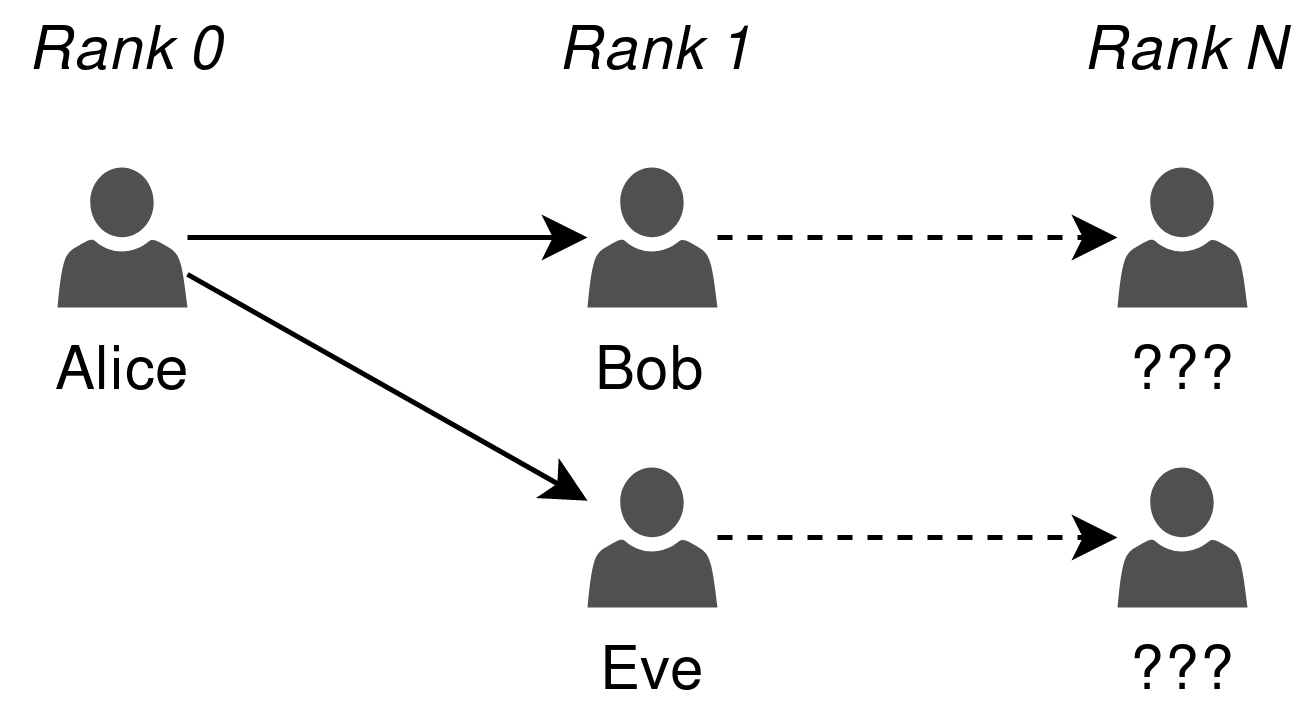
\includegraphics[width=0.7\linewidth]{assets/figures/datcom-fig3} 

}

\caption{Conceptual diagram of scholarly profiles and following others. Network propagation to rank N can be used to facilitate discovery of researchers and to build networks of researchers.}\label{fig:datcom-fig3}
\end{figure}

Using the \texttt{follows} property, Alice can propagate her feed deeper
into her network, as depicted in Figure \ref{fig:datcom-fig3}. More
specifically, Alice's personal profile, rank zero in the network,
extends to the people she follows (i.e., Bob and Eve are rank one).
Subsequently, the profiles Bob and Eve follow are of rank three. By
using recursive functions to crawl the extended network to rank \(N\),
edges in the network are easily discovered despite the (potential) lack
of direct connections (Travers and Milgram
\protect\hyperlink{ref-doi:10.2307ux2f2786545}{1969}).

The \texttt{main} property can be used by a researcher to build a
personalized profile beyond the metadata. For example, Alice wants to
make sure that people who know the Dat link to her scholarly profile can
access her Curriculum Vitae, so she adds \texttt{/cv.pdf} as the
\texttt{main} to her scholarly profile. Whenever she submits a job
application, she can link to her versioned scholarly profile (e.g.,
\texttt{dat://b49...551+13}). Afterwards, she can keep updating her
profile whatever way she likes. She could even choose to host her
website on the decentralized Web by attaching a personal webpage with
\texttt{/index.html}. Because of the versioned link and the properties
of the Dat protocol, she can rest assured that the version she submitted
is the version the reviewing committee sees. Vice versa, whenever she
receives a versioned link to a scholarly profile, she can rest assured
it is what the researcher wanted her to see.

The \texttt{modules} property contains an array of versioned Dat links
to scholarly modules. What these scholarly modules are and how they are
shaped is explained in the next section. The \texttt{modules} property
differs from the \texttt{follows} property in that it can only contain
versioned Dat links, which serve as registrations of the outputs of the
researcher. Where a versioned link in the \texttt{follows} property is
regarded as a \enquote{freeze follow,} a versioned link in the
\texttt{modules} property is the registration and public communication
of the output. The versioned links also prevent duplicate entries of
outputs that are repeatedly updated. For example, a scholarly module
containing a theory could be registered repeatedly over the timespan of
several days or years. If the researcher would register non-versioned
links of the scholarly module, registration would not be specific and
the scholarly profile could contain duplicates. By including only
versioned links the registrations are specific and unique.

\subsection{Scholarly modules}\label{scholarly-modules}

Scholarly research is composed of time-dependent pieces of information
(i.e., modules) that chronologically follow each other. For example,
predictions precede data and results, otherwise they become
postdictions. In a typical theory-testing research study, which adheres
to the framework of a modern empirical research cycle (De Groot
\protect\hyperlink{ref-isbn:9789023228912}{1994}), we can identify at
least eight chronological modules of research outputs: (1) theory, (2)
predictions, (3) study design, (4) study materials, (5) data, (6) code
for analysis, (7) results, (8) discussion, and (9) summary (these are
examples and modules should not be limited to these to prevent
homogenization of scholarly outputs; Star
\protect\hyperlink{ref-doi:10.1111ux2fj.1467-954x.1990.tb03347.x}{1990}).
Sometimes we might iterate between steps, such as adjusting a theory due
to insights gathered when formulating the predictions. Continuously
communicating these in the form of modules as they are produced, by
registering versioned references to Dat filesystems in a scholarly
profile as explained before, could fulfill the five functions of a
scholarly communication system and is unconstrained by the current
article-based system (see also Hartgerink and Zelst
\protect\hyperlink{ref-doi:10.3390ux2fpublications6020021}{2018}).

These scholarly modules each live in their own filesystem, first on the
researcher's computer and when synchronized, on the Dat network. Hence,
researchers can interact with files on their own machine as they are
used to. The Dat network registers changes in the filesystem as soon as
it is activated. As such, researchers can initialize a Dat filesystem on
their computer and, for example, copy private information into the
filesystem, anonymize it and only then activate and synchronize it with
the Dat network (note: this does not require connection to the Internet,
but initialization of the protocol). The private information will then
not be available in the version history of the Dat filesystem.

Metadata for scholarly modules also consists of a generic
\texttt{dat.json} and a more specific \texttt{scholarly-metadata.json}.
The \texttt{dat.json} contains the title of the module, the description,
and its own Dat link. For example, Alice communicates the first module
on the network, where she proposes a theory; the \texttt{dat.json} file
for this module is

\begin{Shaded}
\begin{Highlighting}[]
\FunctionTok{\{}
  \DataTypeTok{"title"}\FunctionTok{:} \StringTok{"Mock Theory"}\FunctionTok{,}
  \DataTypeTok{"description"}\FunctionTok{:} \StringTok{"This is a mock theory but it could just as well }
\StringTok{    be a real one."}\FunctionTok{,}
  \DataTypeTok{"url"}\FunctionTok{:} \StringTok{"dat://dbf...d82"}
\FunctionTok{\}}
\end{Highlighting}
\end{Shaded}

Again, more specific metadata about the decentralized scholarly module
is added in \texttt{scholarly-metadata.json}. As the bare minimum, the
metadata for a scholarly module is initialized as

\begin{Shaded}
\begin{Highlighting}[]
\FunctionTok{\{}
  \DataTypeTok{"type"}\FunctionTok{:} \StringTok{"scholarly-module"}\FunctionTok{,}
  \DataTypeTok{"url"}\FunctionTok{:} \StringTok{"dat://dbf...d82"}\FunctionTok{,}
  \DataTypeTok{"authors"}\FunctionTok{:} \OtherTok{[}
    \StringTok{"dat://b49...551"}\OtherTok{,}
    \StringTok{"dat://167...a26"}
  \OtherTok{]}\FunctionTok{,}
  \DataTypeTok{"parents"}\FunctionTok{:} \OtherTok{[]}\FunctionTok{,}
  \DataTypeTok{"roots"}\FunctionTok{:} \OtherTok{[]}\FunctionTok{,}
  \DataTypeTok{"main"}\FunctionTok{:} \StringTok{"/theory.md"}
\FunctionTok{\}}
\end{Highlighting}
\end{Shaded}

These metadata indicate aspects that are essential in determining
contents and provenance of the module. First, we specify that it is a
scholarly module in the \texttt{type} property. Second, we specify its
own Dat \texttt{url} for reference purposes. Third, an array of Dat
links in the \texttt{authors} property links to scholarly profiles for
authorship. Subsequently, if the module is the following step of a
previous registered module, we specify the Dat link of the preceding
module(s) in the \texttt{parents} property in the form of a versioned
Dat link. Tracing the parents' parents forms a chronology of findings,
leading ultimately to the \texttt{roots} property. In practice, the
\texttt{roots} property is inherited from the immediate parents. Because
the presented hypothetical module above is the first on the network, it
has no parents or roots. The \texttt{main} property specifies a single
landing page/file of the scholarly module. For a text based scholarly
module, \texttt{main} might be \texttt{/index.html} (or
\texttt{/theory.md} as it is here), whereas for a data module that could
be \texttt{/data.csv}. For more complex modules, a guidebook to navigate
the module could be included. The researcher can also store other
relevant assets in the Dat filesystem, such as converted files or
supporting files. For text based scholarly module, assets could include
figures; for data based scholarly modules assets could include
codebooks.

To register a module into the researcher's profile, the versioned Dat
link is included in the \texttt{modules} array on the profile. More
specifically, when the registration process is initiated, the Dat
filesystem is inspected for the latest version number, which is appended
to the Dat link before it is put in the \texttt{modules} property.
Specifically for Alice's theory, she was at version 19 when she wanted
to register it. This means that \texttt{dat://dbf...d82+19} is appended
to the \texttt{modules} array in her scholarly profile. All the users
who follow Alice get an update that she registered her theory, with a
versioned link that is unique and persistent, referring to exactly the
content Alice registered. Alice can keep updating her theory locally,
without it affecting what the people who follow her see, because it does
not affect version 19. When the module is registered, others can view
the most recent version of the Dat filesystem (e.g., theory) by removing
the version from the Dat link (or view any other synchronized version if
available from the network).

Figure \ref{fig:datcom-fig4} depicts how the scholarly modules relate to
each other (Panel B). The versioned, registered scholarly modules become
the parent and root links in subsequent child modules. For example, a
set of predictions link back to the theory they are distilled from; a
study design links back to the predictions it is planned to test and by
extension to the theory it is based on. Panel B in Figure
\ref{fig:datcom-fig4} conceptually depicts one contained empirical
research cycle registered in this way. The links between versioned
scholarly modules embeds the chronological nature of the research
process in its communication.

\begin{figure}[h]

{\centering 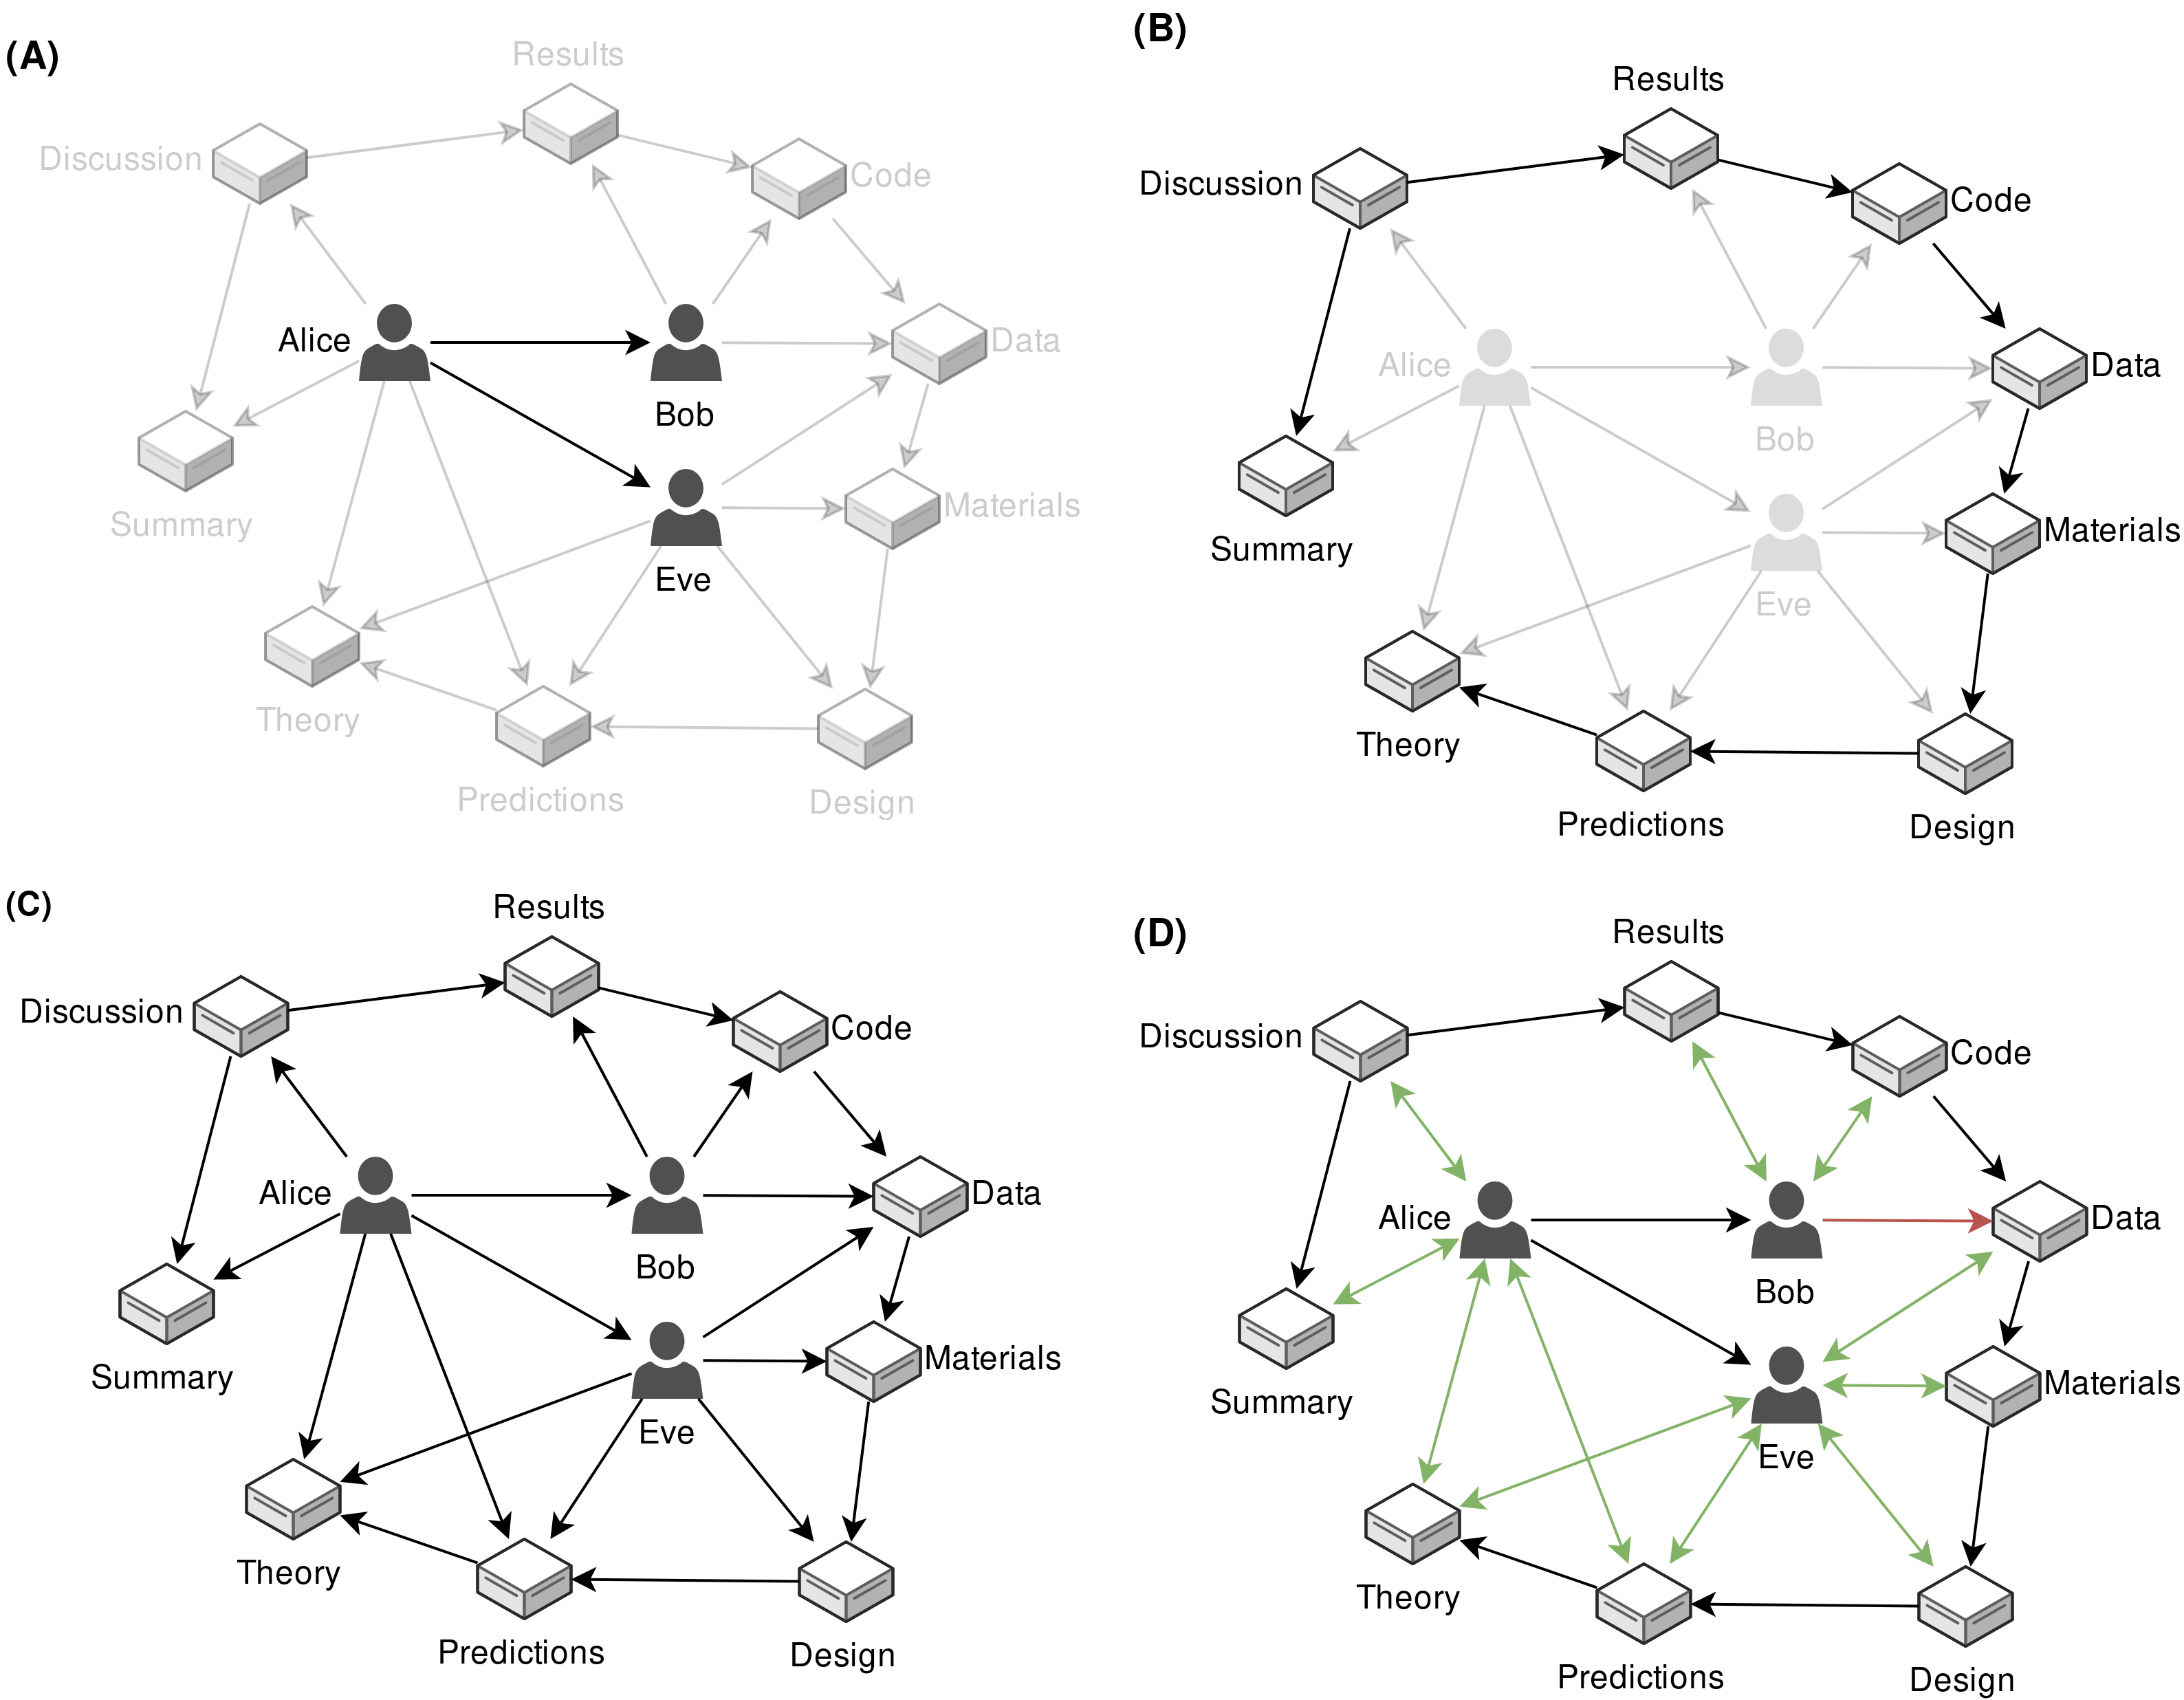
\includegraphics[width=1\linewidth]{assets/figures/datcom-fig4} 

}

\caption{Conceptual representations of how scholarly profiles relate to each other (Panel A), how scholarly modules relate to each other (Panel B), how scholarly profiles and modules create a network of scholarly activity in both researchers and research (Panel C), and how claims of authorship are verified if two-way or unverified if one-way (Panel D).}\label{fig:datcom-fig4}
\end{figure}

\subsection{Verification}\label{verification}

In order to detect whether scholarly modules that a researcher claims to
have authored are indeed (partly) theirs, the scholarly module needs to
also assign the profile as author. For example, Alice and Eve claim to
have authored version 19 of the \enquote{Theory} module in their
profiles (Figure \ref{fig:datcom-fig4}, Panel C). Because a module can
only be edited by its author, we can inspect the scholarly module to
corroborate this. For verified authorship, the module should ascribe
authorship to Alice and Eve. To do this, we inspect
\texttt{scholarly-metadata.json} of the \enquote{Theory} module at the
registered version (i.e., version 19). If the versioned theory module
also ascribes authorship to Alice or Eve, we have two-way verification
of authorship (Figure \ref{fig:datcom-fig4}, Panel D). In other words,
registered scholarly modules must corroborate the authorship claims of
the scholarly profiles in order to become verified.

Unverified authorship can happen when a researcher incorrectly claims
authorship over a module or when a module ascribes authorship to a
researcher who does not claim it. In Figure \ref{fig:datcom-fig4} Panel
D, for example, Bob has claimed authorship of the data module, which is
not corroborated by the scholarly module. Unverified authorship of this
kind (i.e., where a researcher incorrectly claims authorship) is helpful
in preventing misrepresentation of previous work by that researcher.
Unverified authorship where a researcher is incorrectly ascribed
authorship can have various origins. A researcher might remove a
versioned module from their profile, effectively distancing themselves
from the module (similar to retracting the work but on a more individual
level). In a similar vein, it might also be that the author registered a
later version of the module in their profile and deleted the old version
(similar to a corrigendum). Note that the registration will still be
available in the history of the profile, because the history of a Dat
filesystem is append-only.

\subsection{Prototype}\label{prototype}

In order to show that decentralized, modular scholarly communication is
not just a hypothetical exercise, I developed a minimal working
prototype. The prototype code supplied below currently only functions
within Beaker Browser because specific Application Programmatic
Interfaces (APIs) that directly interface with the Dat protocol are not
yet available in the most commonly used Web browsers (e.g., Mozilla
Firefox, Google Chrome).

The minimal working prototype ingests a network of decentralized
scholarly modules and profiles. More specifically, it ingests all
content to rank \(N\) of the network, using
\href{https://github.com/beakerbrowser/webdb}{\texttt{webdb}}.
\texttt{webdb} collects the scholarly metadata from each scholarly
module and scholarly profile and consolidates these disparate pieces of
information into a local database. This database can be considered
temporary; the original information still has its primary origin in the
disparate scholarly modules and scholarly profiles that live on the Dat
network. As such, the same database can be reconstructed at any time
without any issues, assuming the modules are still available. Figure
\ref{fig:datcom-fig5} presents a screenshot of the prototype, which
looks like any other webpage to the user but does not have a centralized
server providing the content. Note also the link at the bottom
showcasing the versioned link to the analysis file.

\begin{figure}[h]

{\centering 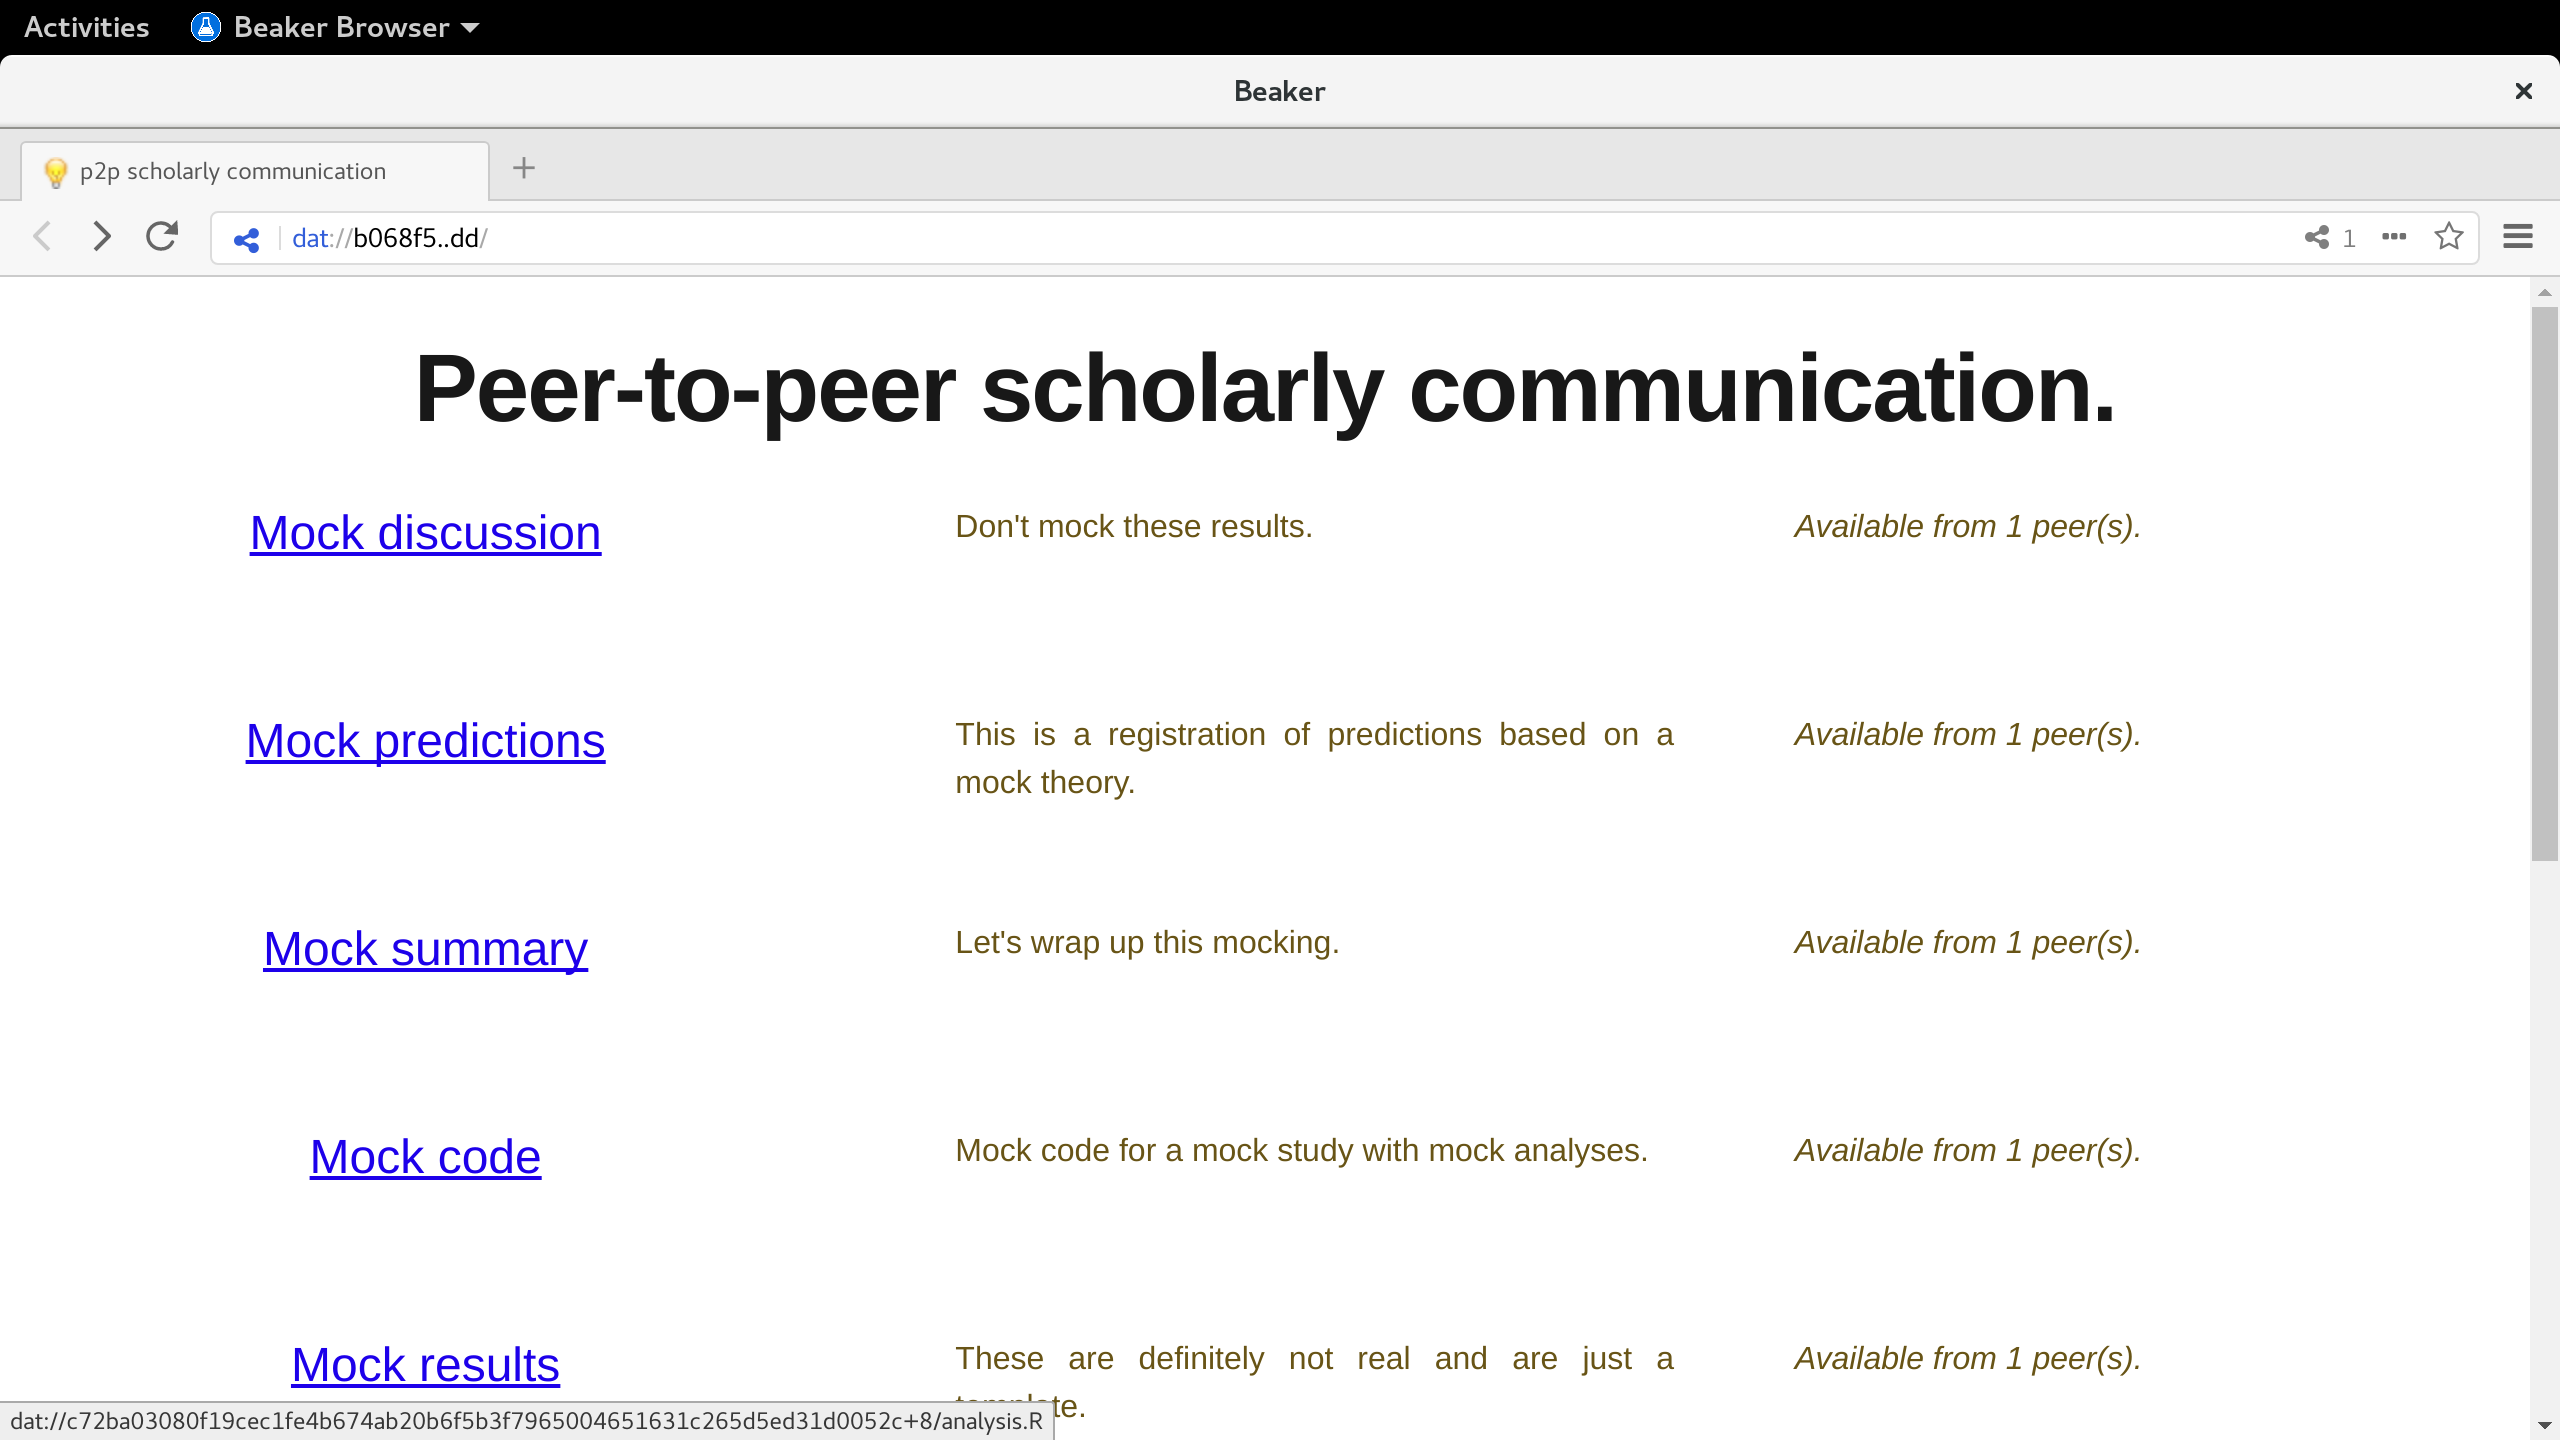
\includegraphics[width=1\linewidth]{assets/figures/datcom-fig5} 

}

\caption{Screencap of the minimal prototype of decentralized scholarly communication. The prototype resembles a regular webpage on the userside, but on the backend it runs entirely on Dat filesystems that live on a decentralized network.}\label{fig:datcom-fig5}
\end{figure}

Procedurally, the prototype takes Alice's scholarly profile as starting
point, subsequently ingesting the network presented in Figure
\ref{fig:datcom-fig4}. By doing so, we get a one-on-one replication of
Alice's perspective (regardless of whether we are Alice or not). As
such, Alice's Dat link serves as the starting point (rank zero). The
metadata contained in her profile is ingested into our local database.
Subsequently, the links in her profile to other scholarly modules (or
profiles) are ingested into the database (rank one), and the links they
have (rank two), and so on (to rank \(N\)). The following JavaScript
code produces this local database for Alice specifically
(\texttt{dat://b49...551}) but can be replaced with Bob's, Eve's, or
anyone else's scholarly profile to receive their personal network.

\begin{Shaded}
\begin{Highlighting}[]
\CommentTok{// npm install -g @beaker/webdb}
\KeywordTok{const}\NormalTok{ WebDB }\OperatorTok{=} \AttributeTok{require}\NormalTok{(}\StringTok{'@beaker/webdb'}\NormalTok{)}

\KeywordTok{let}\NormalTok{ webdb }\OperatorTok{=} \KeywordTok{new} \AttributeTok{WebDB}\NormalTok{(}\StringTok{'view'}\NormalTok{)}

\VariableTok{webdb}\NormalTok{.}\AttributeTok{define}\NormalTok{(}\StringTok{'modules'}\OperatorTok{,} \OperatorTok{\{}
    \DataTypeTok{filePattern}\OperatorTok{:}\NormalTok{ [  }\StringTok{'/scholarly-metadata.json'}\NormalTok{  ]}\OperatorTok{,}
    \DataTypeTok{index}\OperatorTok{:}\NormalTok{ [ }\StringTok{'type'}\OperatorTok{,} \StringTok{'authors'}\OperatorTok{,} \StringTok{'parents'}\OperatorTok{,} \StringTok{'root'}\OperatorTok{,}
     \StringTok{'main'}\OperatorTok{,} \StringTok{'follows'}\OperatorTok{,} \StringTok{'modules'}\NormalTok{ ]}
\OperatorTok{\}}\NormalTok{)}

\NormalTok{async }\KeywordTok{function} \AttributeTok{ingestPortal}\NormalTok{ (url) }\OperatorTok{\{}
\NormalTok{  await }\VariableTok{webdb}\NormalTok{.}\AttributeTok{open}\NormalTok{()}

  \KeywordTok{let}\NormalTok{ archive }\OperatorTok{=} \KeywordTok{new} \AttributeTok{DatArchive}\NormalTok{(url)}
\NormalTok{  await }\VariableTok{webdb}\NormalTok{.}\AttributeTok{indexArchive}\NormalTok{(url)}
  
  \KeywordTok{let}\NormalTok{ scholRaw }\OperatorTok{=}\NormalTok{ await }\VariableTok{archive}\NormalTok{.}\AttributeTok{readFile}\NormalTok{(}
    \StringTok{'/scholarly-metadata.json'}\NormalTok{)}
  
  \KeywordTok{let}\NormalTok{ scholParsed }\OperatorTok{=}\NormalTok{ await }\VariableTok{JSON}\NormalTok{.}\AttributeTok{parse}\NormalTok{(}
\NormalTok{    scholRaw)}
  
  \ControlFlowTok{if}\NormalTok{ (}\VariableTok{scholParsed}\NormalTok{.}\AttributeTok{type} \OperatorTok{===} \StringTok{'scholarly-profile'}\NormalTok{) }\OperatorTok{\{}
    \VariableTok{console}\NormalTok{.}\AttributeTok{log}\NormalTok{(scholParsed)}
    \VariableTok{scholParsed}\NormalTok{.}\VariableTok{follows}\NormalTok{.}\AttributeTok{concat}\NormalTok{(}
      \VariableTok{scholParsed}\NormalTok{.}\AttributeTok{modules}\NormalTok{).}\AttributeTok{forEach}\NormalTok{((val) }\OperatorTok{=>} \OperatorTok{\{}
      \AttributeTok{ingestPortal}\NormalTok{(val)}
    \OperatorTok{\}}\NormalTok{)}
  \OperatorTok{\}}
\OperatorTok{\}}

\AttributeTok{ingestPortal}\NormalTok{(}\StringTok{"dat://b49...551"}\NormalTok{)}
\end{Highlighting}
\end{Shaded}

The presented prototype provides a portal to the information contained
in the modules, but is not the sole portal to access that information.
Because the modules live on a decentralized network and are
open-by-design, anyone may build a portal to view that information
(Figure \ref{fig:datcom-fig6} presents a mockup of an additional
interface). As such, this is not a proposal for a platform but for
infrastructure. The difference between platforms and infrastructure is
vital in light of ownership and responsibility of communicated content
and the moderation of that content. As opposed to centralized services
that carry the legal burden and therefore moderate its platform, this
type of infrastructure does not take such a role and merely aims to
facilitate the individual. As a consequence, the legal burden remains
with the individual. Moreover, platforms require people to go to one
place (e.g., you cannot view content of ResearchGate on Academia.edu or
Elsevier's content on Wiley's webpage); this infrastructure would give
the potential for various types of usage to take place on the same type
of infrastructure.

\begin{figure}
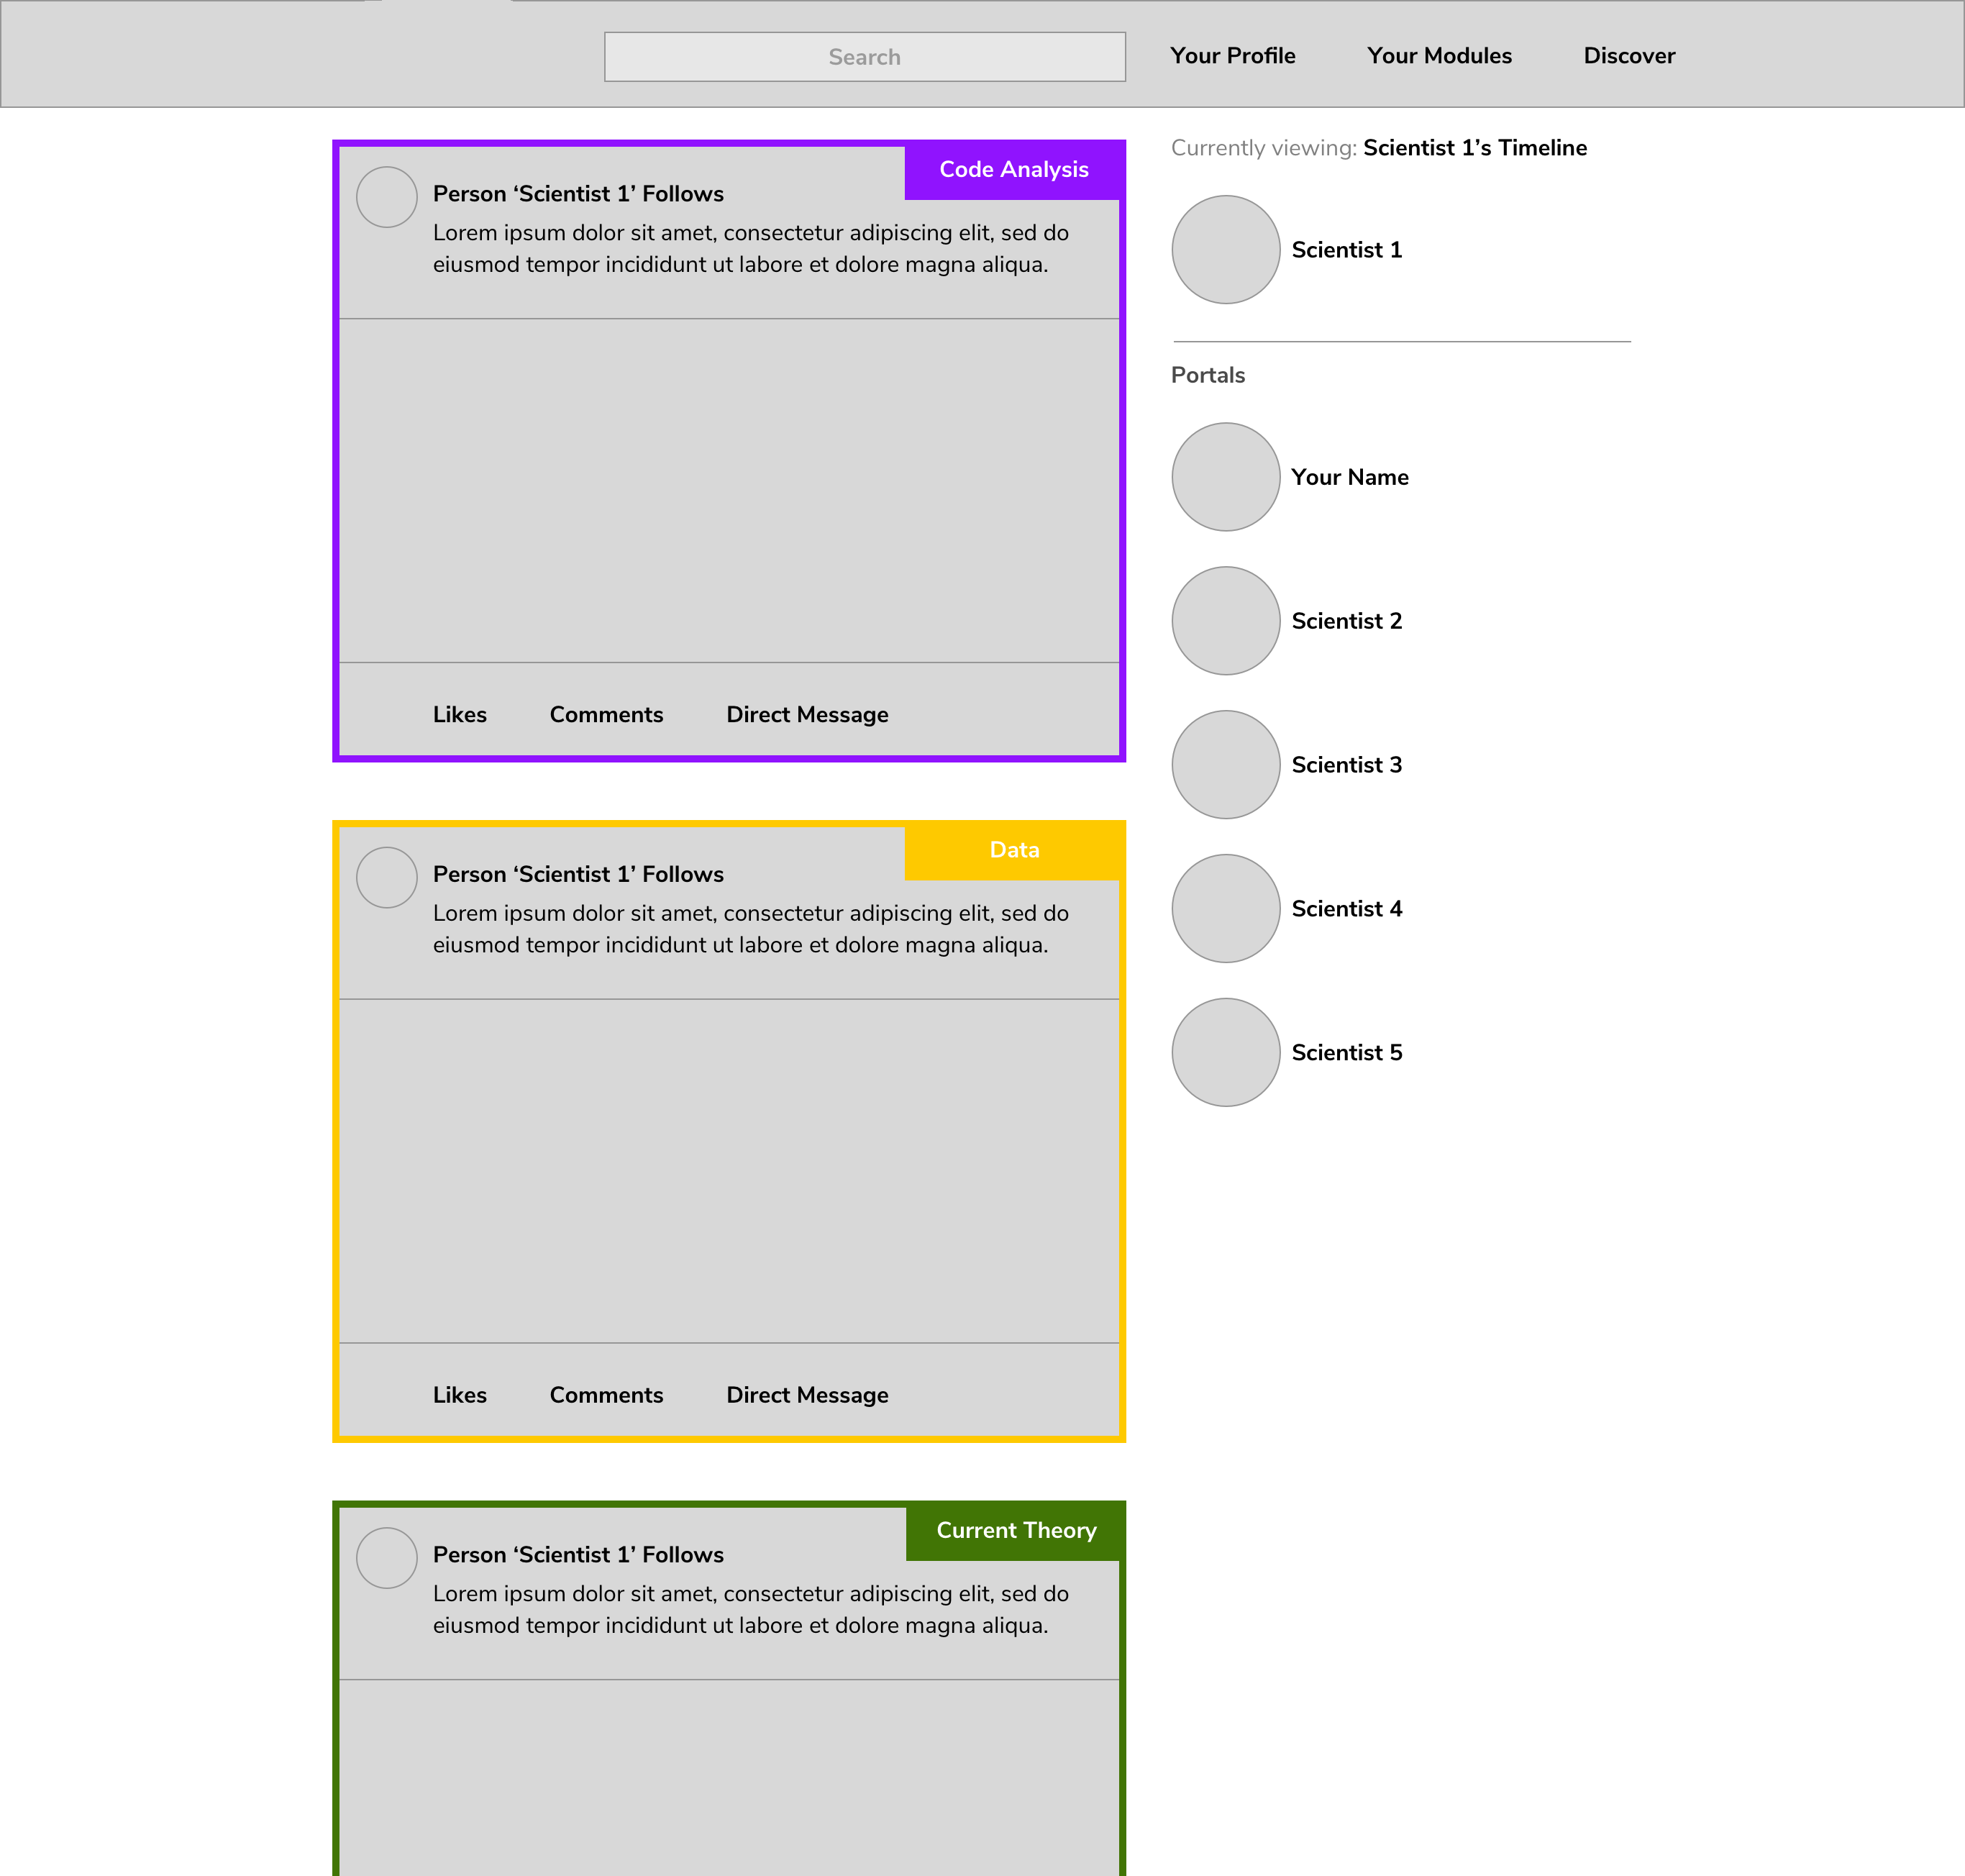
\includegraphics[width=1\linewidth]{assets/figures/datcom-mockup} \caption{Mockup design of an additional interface for the proposed scholarly communication infrastructure. Made by Rebecca Lam, reused under CC-BY 4.0 license.}\label{fig:datcom-fig6}
\end{figure}

\section{Discussion}\label{discussion-8}

The proposed design for decentralized, verified, provenance based
modular communication on the Dat protocol fulfills a wide
conceptualization of the functions of a scholarly communications system
from library and information sciences (Roosendaal and Geurts
\protect\hyperlink{ref-roosendaal1998}{1998}; Sompel et al.
\protect\hyperlink{ref-doi:10.1045ux2fseptember2004-vandesompel}{2004}).
Due to more modular and continuous communication, it is more difficult
to selectively register results when the preceding steps have publicly
been registered already. Moreover, time of communication is decided by
the researcher, making it more feasible for researchers to communicate
their research efforts without biases introduced at the journal stage.
Certification of results is improved by embedding the chronology of the
empirical research cycle in the communication process itself, making
peer-to-peer discussion constructive and less obstructed by hindsight
bias (Nickerson
\protect\hyperlink{ref-doi:10.1037ux2f1089-2680.2.2.175}{1998}).
Unfettered awareness of research is facilitated by using an
open-by-design infrastructure that is the peer-to-peer Dat protocol.
Moreover, because all content is open-by-design and independent of
service platforms, text- and data-mining may be applied freely without
technical restrictions by service providers. The removal of these
technical and service restrictions may facilitate innovations in
discovery of content and the potential for new business models to come
into existence. Based on the links between scholarly modules, the
arising network structure can be used to help evaluate networks of
research(ers) instead of counting publications and citations (Hartgerink
and Zelst
\protect\hyperlink{ref-doi:10.3390ux2fpublications6020021}{2018}).
Archival is facilitated by making it trivially easy to create local
copies of large sets of content, facilitating the Lots Of Copies Keeps
Stuff Safe (LOCKSS; Reich and Rosenthal
\protect\hyperlink{ref-doi:10.1045ux2fjune2001-reich}{2001}; Domenico
and Arenas
\protect\hyperlink{ref-doi:10.1103ux2fphysreve.95.022313}{2017})
principle to be more widely used than just approved organizations.
Moreover, with append-only registers, the provenance of content can also
be archived more readily than it is now. These functions also apply to
non-empirical research that requires provenance of information (e.g.,
qualitative studies).

By producing scholarly content on a decentralized infrastructure,
diversity of how research is consumed and discovered can be facilitated.
Currently, content lives on the webserver of the publisher and is often
solely served at the publisher's webpage due to copyright restrictions
(except for open access articles; Piwowar et al.
\protect\hyperlink{ref-doi:10.7717ux2fpeerj.4375}{2018}). If the design
of the publisher's webpage does not suit the user's needs (e.g., due to
red color blindness affecting approximately 1 in 20 males and 1 in 100
females; Fareed, Anwar, and Afzal
\protect\hyperlink{ref-doi:10.1016ux2fj.gendis.2015.02.006}{2015}),
there is relatively little a user can do. Moreover, service providers
that are not the rightsholder (i.e., publisher) now cannot fulfill that
need for users. By making all content open by default, building on
content becomes easier. For example, someone can build a portal that
automatically shows content with color shifting for people who have red
(or other types of) color blindness. Building and upgrading automated
translation services are another way of improving accessibility (e.g.,
\href{http://translexy.com/}{translexy.com/}), which is currently
restricted due to copyright. Other examples of diverse ways of consuming
or discovering research might include text-based comparisons of modules
to build recommender algorithms that provide contrasting and
corroborating views to users (e.g., McKenzie
\protect\hyperlink{ref-doi:10.1038ux2fnature.2017.22163}{2017}).
Stimulating diversity in how to consume and discover content is key to
making scholarly research accessible to as many people as possible and
in order to attempt to keep some pace with the tremendous amount of
information published each year
(\href{https://api.crossref.org/works?filter=type:journal-article,from-pub-date:2017,until-pub-date:2017\&rows=0}{\textgreater{}3
million articles in 2017}). As such, we have collectively passed the
point of being able to comprehend the relevant information and should no
longer strive to eliminate all uncertainty in knowing but find ways to
deal with that uncertainty better (Bridle
\protect\hyperlink{ref-isbn:9781786635471}{2018}). As such, alternatives
in consuming, discovering, and learning about knowledge are a necessity.
Open Knowledge Maps is an existing example of an innovative discovery
mechanism based on openly licensed and machine-readable content (Kraker,
Kittel, and Enkhbayar
\protect\hyperlink{ref-doi:10.12685ux2f027.7-4-2-157}{2016}). There
would be more smaller pieces of information in the scholarly modules
approach than in the scholarly article approach, which is
counterbalanced by the network structure and lack of technical
restrictions to build tools to digest that information --- this may make
those larger amounts of smaller units (i.e., modules) more digestible
than the smaller volume of larger units (i.e., articles), mitigating
information onslaught (Spellman
\protect\hyperlink{ref-doi:10.1080ux2f1047840X.2012.701161}{2012}).

The proposed design is only the first in a multi-layer infrastructure
that would need to be developed moving forward. Currently, I only
provide a model on the container format for how to store metadata for
modules --- not how the data is stored in the module itself or how the
individual could go about doing so. Moreover, how could reviews be
structured to fit in such modules? As such, the next layer to the
proposed infrastructure would require further specification of how
contents are stored. For example, for text-based modules, what file
formats should be the standard or allowed? It would be unfeasible to
allow any file format due to readability into the future (e.g., Word
2003 files are likely to be problematic) and issues could exacerbate if
software becomes more proprietary and research uses more types of
software. Standards similar to current publications could prove
worthwhile for text (i.e., JATS XML), but impractical to non-technical
users. As such, does the original file need to be in JATS XML when it
can also easily be converted? (e.g., Markdown to JATS XML; Johnston
\protect\hyperlink{ref-jatdown}{2016}) Other specifications for data,
code, materials would also be needed moving forward (e.g., no
proprietary binary files such as SPSS data files). In order to make
those standards practical to individuals not privy to the technical
details, the next infrastructure layer would be building user-facing
applications that interface with the Dat protocol and take the
requirements into account. These would then do the heavy lifting for the
users, guiding them through potential conversion processes and reducing
friction as much as possible. An example of a rich editing environment
that takes the machine readability of scholarly text to the next level,
and makes this relatively easy to the end-user, is Dokie.li (which
writes to HTML; Capadisli et al. \protect\hyperlink{ref-dokieli}{2017}).
This editing environment provides a What You See Is What You Get
(WYSIWYG) editor, while at the same time providing semantic enrichments
to the text (e.g., discerning between positive, negative, corroborating,
or other forms of citations).

New infrastructure layers could provide a much needed upgrade to the
security of scholarly communication. Many of the scholarly publisher's
websites do not use an appropriate level of security in transferring
information to and from the user. More specifically, only 26\% of all
scholarly publishers use HTTPS (Hartgerink
\protect\hyperlink{ref-https-hartgerink}{2018}). This means that any
information transferred to or from the user can be grabbed by anyone in
the physical proximity of that person (amongst other scenarios) ---
including usernames and passwords. In other words, publisher's lack of
up-to-date security practices put the user at risk, but also the
publisher. Some publishers for example complained about Sci-Hub,
alleging that it illegally retrieved articles by phishing researcher's
credentials. A lack of HTTPS would facilitate the illegal retrieval of
user credentials, hence those publishers would ironically facilitate the
kinds of activities they say are illegal (Bohannon
\protect\hyperlink{ref-doi:10.1126ux2fscience.aaf5664}{2016}\protect\hyperlink{ref-doi:10.1126ux2fscience.aaf5664}{a}).
Beyond the potential of missed revenue for pay-to-access publishers,
security negligence is worrisome because the accuracy of scholarly
content is at risk. Man-in-the-middle attacks, where a middleman inserts
themselves between the user and the server, can surreptitiously distort
content, with practical effects for scientific practice (e.g., changing
author names) and real life effects for professions using results for
their jobs (e.g., milligram dosages replaced by gram dosages). By
building a scholarly communication infrastructure on top of the Dat
protocol, all communications are encrypted in transit from one end to
the other by default. For the format of communications, scholarly
publishers may currently be unknowing distributors of malware in their
PDFs distributed to (paying) readers. More specifically, an estimated
.3-2\% of scholarly PDFs contain malware (Nissim et al.
\protect\hyperlink{ref-doi:10.3233ux2f978-1-61499-744-3-107}{2017}),
although the types of malware remain ill specified. By implementing
scholarly modules that are converted on the user's system (e.g., JATS
XML, HTML, Markdown), the attack vector on readers of the scholarly
literature can be reduced by moving away from server-side generated
PDFs, which potentially contain clandestine malware.

\section{Limitations}\label{limitations}

In the proposed decentralized, modular scholarly communication system
there is no requirement for scholarly profiles to be linked to their
real-world entities. This means that scholarly profiles may or may not
be identified. For comparison, a link to a identification is also not
mandatory for ORCID identifiers. Moreover, the history of anonymous (or
pseudonymous) communication has a vibrant historical context in
scholarly communication (e.g., Student
\protect\hyperlink{ref-doi:10.1093ux2fbiometux2f6.1.1}{1908}) and should
therefore not be excluded by the infrastructure design. However, some
might view this as a limitation.

One of the major points of debate may be that the scholarly modules are
chronologically ordered only (both internally and externally). As such,
the temporal distance between two actions within a scholarly module or
between two scholarly modules is unknown. Within a scholarly module and
Dat filesystem, chronological append-only actions are more reliable to
register from a technical perspective than time-based append-only
registers. This has its origin in the fact that creation-,
modification-, and last opened times can technically be altered by
willing users (see for example
\href{https://superuser.com/questions/504829}{superuser.com/questions/504829}).
If timestamps are altered, people can fabricate records that seem
genuine and chronological, but are not --- undermining the whole point
of immutable append-only registers. Hardcoded timestamps in the
scholarly metadata would be an even greater risk due to the potential
for direct modification (i.e., it would only require editing the
\texttt{scholarly-metadata.json} file in a text editor). The external
ordering, that is the chronology of scholarly modules, might be gamed as
well. Consider the scenario where a predictions module at version 12 is
said to be the parent of a design module at version 26 but does not
exist yet at the time of registration for the design module. An
individual with malicious intentions might do this and retroactively
fabricate the parent predictions. So, despite a specific, persistent,
and unique parent Dat link being provided, the chronology could be
undermined, which in turn threatens the provenance of information. It
would require some effort from said researcher to subsequently ensure
that the referenced Dat link contains the postdictions, but it might be
possible to fake predictions in this manner. Other mechanisms could be
put in place to verify the existence of parent links at the time of
registration (which is technically feasible but would require additional
bodies of trust) or to technically investigate for filler actions in a
Dat filesystems when artificially high version numbers are registered.
How to game the proposed system is an active avenue for further
research.

The immutability of the Dat protocol that is central to this proposal
only functions when information is being shared on the network
continuously. Technically, if information has not been shared yet, a
user could check out an old version and create an alternative history.
This could prove useful when accidental versions are registered, but
could also provide incorrect provenance. When already shared, the Dat
protocol rejects the content given that it is inconsistent with previous
versions. As such, as long as peers keep sharing a module once its
author shares it, it is difficult to corrupt. Ongoing implementations
that add a checksum to the Dat link (e.g.,
\texttt{dat://\textless{}hash\textgreater{}@\textless{}checksum\textgreater{}+\textless{}version\textgreater{}})
could help further reduce this issue.

Despite the potential of building an open-by-design scholarly
infrastructure on top of the Dat protocol, there are also domains where
advances need to be made. Until those advances are made, widespread use
in the form of a scholarly communication system remains impractical and
premature (note that no technical limitations prevent an implementation
of the same modular structure on current technologies, for example
GitHub). These developments can occur asynchronously of the further
development of this scholarly communication infrastructure. Amongst
others, these domains include technical aspects and implementations of
the Dat protocol itself, implementations of APIs built on top of it,
legal exploration of intellectual property on a peer-to-peer network,
privacy issues due to high difficulty of removing content permanently
once communicated, the usability of the proposed scholarly
infrastructure, and how to store information in the modules that is
machine readable but also easy-to-use for individuals.

The Dat protocol is functional, but is currently limited to NodeJS and
single-user write access. Because it is currently only available in
NodeJS, portability of the protocol is currently restricted to
JavaScript environments. An experimental implementation of the Dat
protocol is currently being built \href{https://github.com/datrs}{in
Rust} and \href{https://github.com/datcxx}{in C++}, which would greatly
improve availability of the protocol to other environments. Moreover, by
being restricted to single-user write access, Dat archives are not
really portable across machines or users, although work on multi-user
write (i.e., multiple devices or users)
\href{https://github.com/mafintosh/hyperdb}{has recently been released}.
Other APIs built on top of the Dat protocol that are essential to
building a proposed infrastructure, such as \texttt{webdb}, also need to
be further refined in order to make them worthwhile. For example,
\texttt{webdb} currently does not index versioned Dat links but simply
the most recent versions. As such, the indexing of versioned references
is problematic at the moment, but can be readily tackled with further
development. If these and other developments continue, the benefits of
the protocol will mature, may become readily available to individuals
from within their standard browser, and become more practical to
collaborate on. Considering this, the proposed design is imperfect but
timely, allowing for community driven iterations into something more
refined as implementations of the Dat protocol are also refined and may
become more widely used.

Instead of logging in with passwords, the Dat protocol uses
cryptographical verification using a public-private key pair. A
public-private key pair is similar to the lock-key pair we know from
everyday life. This also means that if the (private) key is lost, a
researcher can get locked out from their profile. Similarly, if the
(private) key gets stolen, it might give access to people other than the
researcher. How to securely handle private keys in a user-friendly
manner is an important issue in further development of this scholarly
communication system. Regardless, this changes the threat model from
centralized leaks (for example of plaintext passwords by Elsevier;
\url{https://perma.cc/6J9D-ZPAW}) decentralized security. This would
make the researcher more in control, but also more responsible, for
their operational security.

Despite the Dat protocol's peer-to-peer nature, intellectual property
laws still ascribe copyright upon creation and do not allow copying of
content except when explicitly permitted through non-restrictive
licenses by authors (Baldwin
\protect\hyperlink{ref-isbn:9781400851911}{2014}). As such, intellectual
property laws could be used to hamper widespread copying when licensing
is neglected by authors. Legal uncertainty here might give rise to a
chilling effect to use the Dat protocol to share scholarly information.
Moreover, it seems virtually impossible to issue takedown notices for
(retroactively deemed) illicit content on the Dat protocol without
removing all peer copies on the network. As a result of this, social
perception of the Dat protocol might turn negative if high-profile cases
of illicit or illegal sharing occur (regardless of whether that is
scholarly information or something else). However, just as the Web
requires local copies in cache to function and which lawmakers made
legal relatively quickly when the Web was becoming widespread, the wider
implementation of peer-to-peer protocols to share content might also
require reforms to allow for more permissive copying of original content
shared on the network. Regardless, legal issues need to be thought about
beforehand and users should be made aware that they carry responsibility
for their shared content. Given its inherent open and unrestricted
sharing design, it would make sense to use non-restrictive licenses on
the scholarly modules by default to prevent these legal issues for
researchers wanting to reuse and build on scholarly modules.

Similarly, we need to take seriously the issue that information on the
network, once copied by a peer or multiple peers, is increasingly
unlikely to be uncommunicated. The implications of this in light of
privacy legislations, ethical ramifications, and general negative
effects should not be underestimated. Because a Dat filesystem has a
stable public key and stores versions, the content remains available
even if the content is deleted from the filesystem. That is, users could
go to an older version and still find the file that was deleted. The
only way to truly undo the availability of that information is to remove
all existing copies. Hence, it is worthwhile to ask the question whether
scholarly research that is based on personal data should ever be
conducted on the individual level data or whether this should be done on
higher level summaries of relations between variables (e.g., covariance
matrices). How these summaries can be verified, would remain an issue to
tackle. Conversely, the limitation with respect to privacy is also a
benefit with regards to censorship, where information would also be much
harder to censure (in stark contrast to publishers that might be
pressured by governments; Philips
\protect\hyperlink{ref-guardian-cup}{2017}). Moreover, we might start
thinking about the ownership of data in research. In the case of human
subjects research, researchers now collect data and store it, but we
might consider decentralized data collection where human participants
produce their own data locally and simply permit a researcher to ingest
that into an analysis process (creating throwaway databases themselves
with \texttt{webdb} for example). This would in turn return ownership to
the participant and benefit transparency of data generated.

Bandwidth and persistent peers on the Dat protocol are highly correlated
issues that are key to a usable decentralized infrastructure. When there
are few peers on the network, information redundancy is low, content
attrition is (potentially) high, and bandwidth will be limited.
Subsequently, maximum data transfer of 40KB/s may be possible when few
peers with restricted bandwidth are available and are farther removed on
the physical network. Vice versa, in the most optimal scenario data
transfer could reach the maximum of the infrastructure between peers
(e.g., 1GB/s on peers located on an intranet). Considering that
replicating Dat filesystems is relatively easy given storage space, it
could be done by individuals, and (university) libraries seem
particularly qualified and motivated candidates for persistent hosting
of content on the Dat network. These organizations often have
substantial server infrastructure available, would facilitate high data
transfer speeds, and also have a vested interested in preserving
scholarly content. With over 400 research libraries in Europe and over
\href{http://db.aflia.net/list/?q=6\&m=n}{900 academic libraries in
Africa} alone, bandwidth and redundancy of scholarly content could be
addressed if sufficient libraries participate in rehosting content.
Moreover, the peer-to-peer nature would also allow for researchers to
keep accessing content in the same way when the content is rehosted on
the intranet and the wider connection has service interruptions.

The semi-technical proposal for verified, modular, and provenance based
scholarly infrastructure on the Dat protocol synthesizes meta-research,
technical developments of new Web protocols, real-life issues in a lack
of diversity for consuming scholarly research, and library and
information science's perspectives on the five functions scholarly
communication is supposed to fulfill. With this initial proposal a
scholarly commons seems feasible. The proposal provides a more complete
and less biased register of information than the current article-based
system. Moreover, it facilitates more constructive certification
discussions and allows anyone with access to the Internet to
participate. It also provides archival supportive of the distribution,
which anyone may meaningfully contribute to if they have the physical
means. This proposal also may provide new ways of evaluating, consuming,
and discovering research. The decentralized nature of the Dat protocol
requires less trust to be put in institutions to maintain key data
stores that are the fundament to any infrastructure and replaces it with
widespread distribution of that information. However, technological,
legal, and social developments need to occur asynchronously to make this
a reality.

\section{Supporting Information}\label{supporting-information-1}

S1 File. Overview of original Dat links corresponding to shortened
links:
\url{https://github.com/chartgerink/2018dat-com/raw/master/assets/mock-modules-overview.ods}.

\chapter*{Summary}\label{summary}
\addcontentsline{toc}{chapter}{Summary}

This dissertation focuses on either understanding and detecting threats
to the epistemology of science (chapters 1-6) or making practical
advances to remedy epistemological threats (chapters 7-9)

Chapter 1 reviews the literature on responsible conduct of research,
questionable research practices, and research misconduct. Responsible
conduct of research is often defined in terms of a set of abstract,
normative principles, professional standards, and ethics in doing
research. In order to accommodate the normative principles of scientific
research, the professional standards, and a researcher's moral
principles, transparent research practices can serve as a framework for
responsible conduct of research. Here I suggest a
\enquote{prune-and-add} project structure to enhance transparency and by
extension, responsible conduct of research. Questionable research
practices are defined as practices that are detrimental to the research
process. The prevalence of questionable research practices remains
largely unknown and reproducibility of findings has been shown to be
problematic. Questionable practices are discouraged by transparent
practices because practices that arise from them will become more
apparent to scientific peers. Most effective might be preregistrations
of research design, hypotheses, and analyses, which reduce particularism
of results by providing an a priori research scheme. Research misconduct
has been defined as fabrication, falsification, and plagiarism (FFP),
which is clearly the worst type of research practice. Despite it being
clearly wrong, it can be approached from a scientific and legal
perspective. The legal perspective sees research misconduct as a form of
white-collar crime. The scientific perspective seeks to answer the
question \enquote{were results invalidated because of the misconduct?} I
review how misconduct is typically detected, how its detection can be
improved, and how prevalent it might be. Institutions could facilitate
detection of data fabrication and falsification by implementing data
auditing. Nonetheless, the effect of misconduct is pervasive: many
retracted articles are still cited after the retraction has been issued.

Head et al.
(\protect\hyperlink{ref-doi:10.1371ux2fjournal.pbio.1002106}{2015}\protect\hyperlink{ref-doi:10.1371ux2fjournal.pbio.1002106}{b})
provided a large collection of \(p\)-values that, from their
perspective, indicates widespread statistical significance seeking
(i.e., \(p\)-hacking). Chapter 2 inspects this result for robustness.
Theoretically, the \(p\)-value distribution should be a smooth,
decreasing function, but the distribution of reported \(p\)-values shows
systematically more reported \(p\)-values for .01, .02, .03, .04, and
.05 than \(p\)-values reported to three decimal places, due to apparent
tendencies to round \(p\)-values to two decimal places. Head et al.
(\protect\hyperlink{ref-doi:10.1371ux2fjournal.pbio.1002106}{2015}\protect\hyperlink{ref-doi:10.1371ux2fjournal.pbio.1002106}{b})
correctly argue that an aggregate \(p\)-value distribution could show a
bump below .05 when left-skew \(p\)-hacking occurs frequently. Moreover,
the elimination of \(p=.045\) and \(p=.05\), as done in the original
paper, is debatable. Given that eliminating \(p=.045\) is a result of
the need for symmetric bins and systematically more \(p\)-values are
reported to two decimal places than to three decimal places, I did not
exclude \(p=.045\) and \(p=.05\). I applied Fisher's method on
\(.04<p<.05\) and reanalyzed the data by adjusting the bin selection to
\(.03875<p\leq.04\) versus \(.04875<p\leq.05\). Results of the
reanalysis indicate that no evidence for left-skew \(p\)-hacking remains
when I look at the entire range between \(.04<p<.05\) or when I inspect
the second-decimal. Taking into account reporting tendencies when
selecting the bins to compare is especially important because this
dataset does not allow for the recalculation of the \(p\)-values.
Moreover, inspecting the bins that include two-decimal reported
\(p\)-values potentially increases sensitivity if strategic rounding
down of \(p\)-values as a form of \(p\)-hacking is widespread. Given the
far-reaching implications of supposed widespread \(p\)-hacking
throughout the sciences Head et al.
(\protect\hyperlink{ref-doi:10.1371ux2fjournal.pbio.1002106}{2015}\protect\hyperlink{ref-doi:10.1371ux2fjournal.pbio.1002106}{b}),
it is important that these findings are robust to data analysis choices
if the conclusion is to be considered unequivocal. Although no evidence
of widespread left-skew \(p\)-hacking is found in this reanalysis, this
does not mean that there is no \(p\)-hacking at all. These results
nuance the conclusion by Head et al.
(\protect\hyperlink{ref-doi:10.1371ux2fjournal.pbio.1002106}{2015}\protect\hyperlink{ref-doi:10.1371ux2fjournal.pbio.1002106}{b}),
indicating that the results are not robust and that the evidence for
widespread left-skew \(p\)-hacking is ambiguous at best.

Chapter 3 examined 258,050 test results across 30,710 articles from
eight high impact journals to investigate the existence of a peculiar
prevalence of \(p\)-values just below .05 (i.e., a bump) in the
psychological literature, and a potential increase thereof over time. I
indeed found evidence for a bump just below .05 in the distribution of
exactly reported \(p\)-values in the journals Developmental Psychology,
Journal of Applied Psychology, and Journal of Personality and Social
Psychology, but the bump did not increase over the years and disappeared
when using recalculated \(p\)-values. I found clear and direct evidence
for the QRP \enquote{incorrect rounding of \(p\)-value} (John,
Loewenstein, and Prelec
\protect\hyperlink{ref-doi:10.1177ux2f0956797611430953}{2012}) in all
psychology journals. Finally, I also investigated monotonic excess of
\(p\)-values, an effect of certain QRPs that has been neglected in
previous research, and developed two measures to detect this by modeling
the distributions of statistically significant \(p\)-values. Using
simulations and applying the two measures to the retrieved test results,
I argue that, although one of the measures suggests the use of QRPs in
psychology, it is difficult to draw general conclusions concerning QRPs
based on modeling of \(p\)-value distributions.

In Chapter 4 I examined evidence for false negatives in nonsignificant
results in three different ways. I adapted the Fisher method to detect
the presence of at least one false negative in a set of statistically
nonsignificant results. Simulations show that the adapted Fisher method
generally is a powerful method to detect false negatives. I examined
evidence for false negatives in the psychology literature in three
applications of the adapted Fisher method. These applications indicate
that (i) the observed effect size distribution of nonsignificant effects
exceeds the expected distribution assuming a null-effect, and
approximately two out of three (66.7\%) psychology articles reporting
nonsignificant results contain evidence for at least one false negative,
(ii) nonsignificant results on gender effects contain evidence of true
nonzero effects, and (iii) the statistically nonsignificant replications
from the Reproducibility Project Psychology (RPP) do not warrant strong
conclusions about the absence or presence of true zero effects
underlying these nonsignificant results. I conclude that false negatives
deserve more attention in the current debate on statistical practices in
psychology. Potentially neglecting effects due to a lack of statistical
power can lead to a waste of research resources and stifle the
scientific discovery process.

Chapter 5 describes a dataset that is the result of content mining
167,318 published articles for statistical test results reported
according to the standards prescribed by the American Psychological
Association (APA). Articles published by the APA, Springer, Sage, and
Taylor \& Francis were included (mining from Wiley and Elsevier was
actively blocked). As a result of this content mining, 688,112 results
from 50,845 articles were extracted. In order to provide a comprehensive
set of data, the statistical results are supplemented with metadata from
the article they originate from. The dataset is provided in a comma
separated file (CSV) in long-format. For each of the 688,112 results, 20
variables are included, of which seven are article metadata and 13
pertain to the individual statistical results (e.g., reported and
recalculated \(p\)-value). A five-pronged approach was taken to generate
the dataset: (i) collect journal lists; (ii) spider journal pages for
articles; (iii) download articles; (iv) add article metadata; and (v)
mine articles for statistical results. All materials, scripts, etc. are
available at
\url{https://github.com/chartgerink/2016statcheck_data}\footnote{This
  GitHub repository has been deleted since this chapter was previously
  published. The links are included to remain consistent with the
  published version.} and preserved at
\href{http://doi.org/10.5281/zenodo.59818}{http://dx.doi.org/10.5281/zenodo.59818}.

In Chapter 6, I test the validity of statistical methods to detect
fabricated data in two studies. In Study 1, I tested the validity of
statistical methods to detect fabricated data at the study level using
summary statistics. Using (arguably) genuine data from the Many Labs 1
project on the anchoring effect (\(k=36\)) and fabricated data for the
same effect by our participants (\(k=39\)), I tested the validity of our
newly proposed \enquote{reversed Fisher method}, variance analyses, and
extreme effect sizes, and a combination of these three indicators using
the original Fisher method. Results indicate that the variance analyses
perform fairly well when the homogeneity of population variances is
accounted for and that extreme effect sizes perform similarly well in
distinguishing genuine from fabricated data. The performance of the
\enquote{reversed Fisher method} was poor and depended on the types of
tests included. In Study 2, I tested the validity of statistical methods
to detect fabricated data using raw data. Using (arguably) genuine data
from the Many Labs 3 project on the classic Stroop task (\(k=21\)) and
fabricated data for the same effect by our participants (\(k=28\)), I
investigated the performance of digit analyses, variance analyses,
multivariate associations, and extreme effect sizes, and a combination
of these four methods using the original Fisher method. Results indicate
that variance analyses, extreme effect sizes, and multivariate
associations perform fairly well to excellent in detecting fabricated
data using raw data, while digit analyses perform at chance levels. The
two studies provide mixed results on how the use of random number
generators affects the detection of data fabrication. Ultimately, I
consider the variance analyses, effect sizes, and multivariate
associations valuable tools to detect potential data anomalies in
empirical (summary or raw) data. However, I argue against widespread
(possible automatic) application of these tools, because some fabricated
data may be irregular in one aspect but not in another. Considering how
violations of the assumptions of fabrication detection methods may yield
high false positive or false negative probabilities, I recommend
comparing potentially fabricated data to genuine data on the same topic.

Chapter 7 tackles the issue of data extraction. It is common for authors
to communicate their results in graphical figures, but those data are
frequently unavailable for reanalysis. Reconstructing data points from a
figure manually requires the author to measure the coordinates either on
printed pages using a ruler, or from the display screen using a cursor.
This is time-consuming (often hours) and error-prone, and limited by the
precision of the display or ruler. What is often not realised is that
the data themselves are held in the PDF document to much higher
precision (usually 0.0-0.01 pixels), if the figure is stored in vector
format. We developed alpha software to automatically reconstruct data
from vector figures and tested it on funnel plots in the meta-analysis
literature. Our results indicate that reconstructing data from vector
based figures is promising, where I correctly extracted data for 12 out
of 24 funnel plots with extracted data (50\%). However, I observed that
vector based figures are relatively sparse (15 out of 136 papers with
funnel plots) and strongly insist publishers to provide more vector
based data figures in the near future for the benefit of the scholarly
community.

Scholarly research faces threats to its sustainability on multiple
domains (access, incentives, reproducibility, inclusivity). In Chapter 8
I argue that \enquote{after-the-fact} research papers do not help and
actually cause some of these threats because the chronology of the
research cycle is lost in a research paper. I propose to give up the
academic paper and propose a digitally native \enquote{as-you-go}
alternative. In this design, modules of research outputs are
communicated along the way and are directly linked to each other to form
a network of outputs that can facilitate research evaluation. This
embeds chronology in the design of scholarly communication and
facilitates recognition of more diverse outputs that go beyond the paper
(e.g., code, materials). Moreover, using network analysis to investigate
the relations between linked outputs could help align evaluation tools
with evaluation questions. I illustrate how such a modular
\enquote{as-you-go} design of scholarly communication could be
structured and how network indicators could be computed to assist in the
evaluation process, with specific use cases for funders, universities,
and individual researchers.

A scholarly communication system needs to register, distribute, certify,
archive, and incentivize knowledge production. Chapter 9 proposes that
the current article-based system technically fulfills these functions,
but suboptimally. I propose a module-based communication infrastructure
that attempts to take a wider view of these functions and optimize the
fulfillment of the five functions of scholarly communication. Scholarly
modules are conceptualized as the constituent parts of a research
process as determined by a researcher. These can be text, but also code,
data, and any other relevant piece of information. The chronology of
these modules is registered by iteratively linking to each other,
creating a provenance record of parent- and child modules (and a network
of modules). These scholarly modules are linked to scholarly profiles,
creating a network of profiles, and a network of profiles and their
constituent modules. All these scholarly modules would be communicated
on the new peer-to-peer Web protocol Dat
(\href{https://datproject.org}{datproject.org}), which provides a
decentralized register that is immutable, facilitates greater content
integrity through verification, and is open by design. Open by design
would also allow diversity in the way content is consumed, discovered,
and evaluated to arise. This initial proposal needs to be refined and
developed further based on technical developments of the Dat protocol
and its implementations, and discussions within the scholarly community
to evaluate the qualities claimed here. Nonetheless, a minimal prototype
is available today and this is technically feasible.

\chapter*{Epilogue}\label{epilogue}
\addcontentsline{toc}{chapter}{Epilogue}

Eight years after my first epistemological crisis, during which I spent
five years attempting to understand and find ways to improve the
sustainability of science, I see no way around it: We need new systems
to intersectionally address the systemic issues of science. Now, most
reform fiddles with minor superficial knobs when and where we are
allowed to. Piecemeal reform, such as giving virtual stickers for
sharing data, is just not going to cut it when we want to do something
about the sustainability of science. In this Epilogue, I reflect on the
dire need for radical and uncompromising reform in science and I propose
a set of demands.

The fundamental question when choosing between reformism and radicalism
is whether one thinks the current system mostly works. Reformist
thinking is conditional on the current system, whereas radical thinking
is unconditioned. In that sense, reformist thinking accepts the very
system it is trying to change --- which makes perfect sense if one
explicitly or implicitly believes the current system mostly works or if
it serves them. Hence, there is a clear interest for established actors
to argue for (conservative) reform. Conversely, radicalism does not
condition itself on the current system and reimagines what is necessary
where it is necessary. I consider that the current system, taken to its
logical conclusion, does not work, hence, is unsustainable. For that
reason, I see radical thinking as the only viable option.

That the current, article based, scientific system is too broken to fix
has become painfully clear. Putting aside how invested the established
institutions are in the current system, why should it objectively
persist in its current form? Not only must all changes to the
publication system, even effective ones, go through the gatekeepers of
that system, those gatekeepers do not even serve the scientific system.
The publishers clearly and logically serve their shareholders in the
end. Even if we could alter the rules such that mischief no longer pays
in the publishing game (Bakker, Dijk, and Wicherts
\protect\hyperlink{ref-doi:10.1177ux2f1745691612459060}{2012}), framing
it in terms of bettering science need not convince publishers. Moreover,
my research suggests that it is unfeasible to detect mischief at large,
indicating it may be more fruitful to aim for a system that prevents it
in the first place. Only under the sunk cost fallacy does it make sense
to me to keep the current system.

In order to understand the need for radical reform from another angle,
we need to consider how the complex systemic issues of science are
intertwined with the complex systemic issues of society. One societal
issue that affects issues in science, for example, is austerity policy
in government spending. Spending cuts affect the available national
(research) budgets, which in turn intensifies competition among
scientists, negatively affecting their mental health\footnote{I am
  afraid this example is all too familiar to many.} and feeding a race
to the bottom of validity of findings (Smaldino and McElreath
\protect\hyperlink{ref-doi:10.1098ux2frsos.160384}{2016}). Vice versa,
we cannot neglect the impact the scientific system has on societal
issues. For example, we increasingly add to the ecological crises
through conference travel as careers advance (Wynes et al.
\protect\hyperlink{ref-doi:10.1016ux2fj.jclepro.2019.04.109}{2019});
labs also produce large amounts of waste (one lab estimates
approximately 1 ton of plastics per researcher per year; Urbina, Watts,
and Reardon \protect\hyperlink{ref-doi:10.1038ux2f528479c}{2015}).

Many complex interactions between issues of science and society exist.
These include restrictive access to publications, causing many people to
resort to illegitimate means to gain access for legitimate purposes
(Bohannon
\protect\hyperlink{ref-doi:10.1126ux2fscience.352.6285.508}{2016}\protect\hyperlink{ref-doi:10.1126ux2fscience.352.6285.508}{b})\footnote{\href{https://therostrumblog.wordpress.com/2015/01/12/why-all-phd-students-should-do-a-policy-placement/}{It
  even happens that governments seek university interns to get access}}.
Additionally, in an attempt to manage the risks Open Access poses to
their subscription models (and shareholders), the highly centralized
oligarchy of academic publishers are shifting to business models
resembling the problematic and data-exploitative models of Facebook. But
even for researchers, the cost to play in publishing Open Access is
substantial and rising faster than inflation (Grossmann and Brembs
\protect\hyperlink{ref-doi:10.7287ux2fpeerj.preprints.27809v1}{2019}),
reaffirming structural and global inequalities. This extends existing
inequalities in participation, such as participation in scientific
education that is increasingly difficult as collective financing
programs are replaced with individualized debt\footnote{Again, due to
  austerity measures of governments.}. These complex issues do not even
begin to grapple with the distortion caused by biased publication of
results. If the studied effects are not large (the low hanging fruit) or
widely reproduced using open data, the rules of the game promote
contradicting results, serving confirmation bias. Moreover, intellectual
property laws restrict our capabilities to deal with information
overload in science. On top of all of this and more, systemic factors
resulting in explicit and implicit individual or institutionalized
ableism, ageism, classism, homophobia, racism, sexism, and transphobia
multiply these struggles for already underrepresented scientists, making
it probable they become even more underrepresented as time passes. How
can we create or expect valid, reproducible, and applicable knowledge if
these issues are its context?

We need to start considering these interconnected issues together, not
separately, and consider that current powerful stakeholders are invested
in maintaining the status quo. Parallel scientific systems provide a
space to envision something totally different. In order to build
parallel systems that may provide hope in this web of complex issues, we
need to integrate the critical study of scientific practices with
critical studies of society, economics, organizations, information
technology, and other relevant fields. Only that way will we be able to
determine and interconnect the issues that need to be addressed in their
broadest sense. Parallel systems also allow us to do more than simply
shift power to a new generation; we can use it to restructure and
distribute power. To restructure power in such a way that when we learn
about the immanent problems of the new systems we build, power longer
serves to maintain the status quo but to change it. To distribute power
such that those traditionally underrepresented may finally become
adequately represented.

What should we demand of a parallel scientific system to make it
worthwhile? The following demands can serve as utopian expectations to
strive towards and evaluate proposals.

A worthwhile scientific system must be widely applicable. It must be
usable on its own, but also in parallel with current structures people
might already be embedded in (e.g., universities). This would allow
simultaneous participation in both old and new systems for researchers
in institutions. This would also not force (early career) academics into
zero-sum publishing decisions, which would effectively exacerbate the
institutionalized issues they are already facing. Nonetheless, the
parallel system should be usable on its own for researchers outside of
academic institutions, who should not be forced to conform to the norms
of the institutions that they are not a part of (or may have actively
rejected if they left academia).

Beyond minimizing barriers to participation in the scientific system,
everyday research practices must be facilitated in the most concrete
way. Too many proposals for change in the scientific system simply add
to the already overburdening research process, making it more, not less,
difficult to do and participate in research. Especially (quick)
technocratic fixes serve such alienation from research: technocrats
formulate these rules to create a veil of progress, telling people what
to do but (often) not how they might go about (effectively) doing so.
Additionally, technocratic measures are inherently institution-specific
and affirm top-down control mechanisms, further entrenching power
inequities. A worthwhile alternative must boost bottom-up change by
making it easier to organize information, retrieve it, discuss it, and
use it in the most concrete, everyday sense.

Alternatives must provide a coherent and extensive answer to the
functions of a scholarly communication system. These functions encompass
access, registration, certification, archival, and incentives. By
analyzing the limitations of the current system on these functions, we
can design an alternative that differentiates itself substantially and
completely. By providing a more coherent and parsimonious answer to
these functions, a parallel system may also prove more convincing for
bottom-up change.

Those designing parallel scientific systems must actively renew and
embed the values in science. As a result, incrementalism, validity,
reliability, and replications must become preferred and rewarded over
innovativeness, unreliability, and spontaneous isolated discovery. There
is nothing objective about what we subjectively decide to value. Only
deep and active value changes allow for incentive superstructures that
substantially differ from the current and problematic system.

Access to- and reuse of information must be complete and unlimited,
further removing barriers to participate in research. Unlimited access
and reuse means that intellectual control and censorship of information
by state, commercial, or other actors needs to be mitigated by design.
These actors benefit from bottlenecks in information flow that can be
tightened, controlled, and surveilled. This is exactly how the services
we now use are (being) designed. Hence, current centralized and
restrictive models need to be replaced for decentralized and permissive
models.

We must demand the potential of unlimited ways to deal with information
overload. Full access and unlimited reuse permits us to deal with
information overload in better ways by making it easier to commodify
ways to consume and discover information. Creating such a market was
part of the European Digital Single Market strategy, but it failed to do
so. Oligarchic control over access and reuse prevents its existence
today. By demanding decentralization and distribution of information, we
may break up both the oligarchic publishing structures in science and
break up the oligarchic control over the data on which services can be
built.

To better deal with information overload we must also demand new
information structures. Transparency is often proposed as the key to
reforming science, but without somewhat standardized structures to make
sense of what is available, there is a risk of obfuscation. I have spent
many hours trying to understand someone else's project structure with
hundreds of files. This does not scale for sustainable information
consumption and production. Questions about the unit of communication
and what is communicable seem timely when the lack of chronology causes
some of the issues in science (e.g., HARKing; Kerr
\protect\hyperlink{ref-doi:10.1207ux2fs15327957pspr0203_4}{1998}). As we
create new information structures, we must also demand schemas that are
flexible enough to allow for heterogeneous forms of research and prevent
excessive rigidity that homogenizes and may even straitjacket research.

Due to the delicate balances and interests that need to be sought, we
must demand that these systems are built in an open, dialectical, and
actively inclusive way. It is unacceptable to create new (temporary)
exclusionary privileges under the header of progress (e.g., the
temporary Open Access privilege the Bill and Melinda Gates Foundation
created; Van Noorden
\protect\hyperlink{ref-doi:10.1038ux2fnature.2017.21486}{2017}). This
means that any form of oligarchic control over how these demands are
implemented needs to be actively prevented and bottom-up procedures need
to actively be promoted.

Finally, we must demand systems that are sustainable for both knowledge
production and the planetary environment. This is \emph{the} acute
societal context that we must not neglect (IPCC
\protect\hyperlink{ref-ipccGlobalWarmingIPCC2018}{2018}). In order to
reduce the need for consumptive resources (often fossil fuel based;
Pirani \protect\hyperlink{ref-isbn:9780745335612}{2018}), we must
reimagine how we can interact with other researchers. Doing so may
drastically reduce the need for flights for conferences (and benefit our
schedules). The digital services that are provided also consume
substantial amounts of energy, especially given the rise of machine
learning algorithms whose training is substantial in its energy use
(Strubell, Ganesh, and McCallum
\protect\hyperlink{ref-DBLP:journalsux2fcorrux2fabs-1906-02243}{2019}).
Any radical proposals must be evaluated on their sustainability given
the acute urgency of the ecological crises.

Only together do these demands produce a framework to build parallel
systems that may start to substantially change the sustainability of
science. Many scientific issues intersect with the societal issues that
we are embedded in; ignoring this intersection harms effective and
sustainable change. Reformist changes often lack this intersectionalism
by being highly specific, which ultimately results in more effort spent
for (maybe) the same goals. Regardless, the described framework served
me in creating a concrete radical proposal (cf.~chapters 8 and 9) and
provides the basis as I implement this in my work moving forward.
Nonetheless, there is a multiplicity of ways to think radically and
achieve these demands. With pluralism of radical ideas, substantial
change may happen. In the end, it does not matter who makes the change,
but that the change happens.

\appendix


\chapter{Examining statistical properties of the Fisher
test}\label{examining-statistical-properties-of-the-fisher-test}

The Fisher test to detect false negatives is only useful if it is
powerful enough to detect evidence of at least one false negative result
in papers with few nonsignificant results. Therefore we examined the
specificity and sensitivity of the Fisher test to test for false
negatives, with a simulation study of the one sample \(t\)-test.
Throughout this chapter, we apply the Fisher test with
\(\alpha_{Fisher}=0.10\), because tests that inspect whether results are
\enquote{too good to be true} typically also use alpha levels of 10\%
(Sterne, Gavaghan, and Egger
\protect\hyperlink{ref-doi:10.1016ux2fs0895-43560000242-0}{2000};
Ioannidis and Trikalinos
\protect\hyperlink{ref-doi:10.1177ux2f1740774507079441}{2007}; Francis
\protect\hyperlink{ref-doi:10.3758ux2fs13423-012-0227-9}{2012}). The
simulation procedure was carried out for conditions in a three-factor
design, where power of the Fisher test was simulated as a function of
sample size \(N\), effect size \(\eta\), and \(k\) test results. The
three factor design was a 3 (sample size \(N\): 33, 62, 119) by 100
(effect size \(\eta\): .00, .01, .02, \ldots{}, .99) by 18 (\(k\) test
results: 1, 2, 3, \ldots{}, 10, 15, 20, \ldots{}, 50) design, resulting
in 5,400 conditions. The levels for sample size were determined based on
the 25th, 50th, and 75th percentile for the degrees of freedom (\(df2\))
in the observed dataset for Application 1. Each condition contained
10,000 simulations. The power of the Fisher test for one condition was
calculated as the proportion of significant Fisher test results given
\(\alpha_{Fisher}=0.10\). If the power for a specific effect size
\(\eta\) was \(\geq99.5\%\), power for larger effect sizes were set to
1.

We simulated false negative \(p\)-values according to the following six
steps (see Figure \ref{fig:appendix5a}. First, we determined the
critical value under the null distribution. Second, we determined the
distribution under the alternative hypothesis by computing the
non-centrality parameter as \(\delta=(\eta^2/1-\eta^2)N\) (Steiger and
Fouladi \protect\hyperlink{ref-Steiger1997-qq}{1997}; Smithson
\protect\hyperlink{ref-doi:10.1177ux2f00131640121971392}{2001}). Third,
we calculated the probability that a result under the alternative
hypothesis was, in fact, nonsignificant (i.e., \(\beta\)). Fourth, we
randomly sampled, uniformly, a value between \(0-\beta\). Fifth, with
this value we determined the accompanying \(t\)-value. Finally, we
computed the \(p\)-value for this \(t\)-value under the null
distribution.

\begin{figure}

{\centering 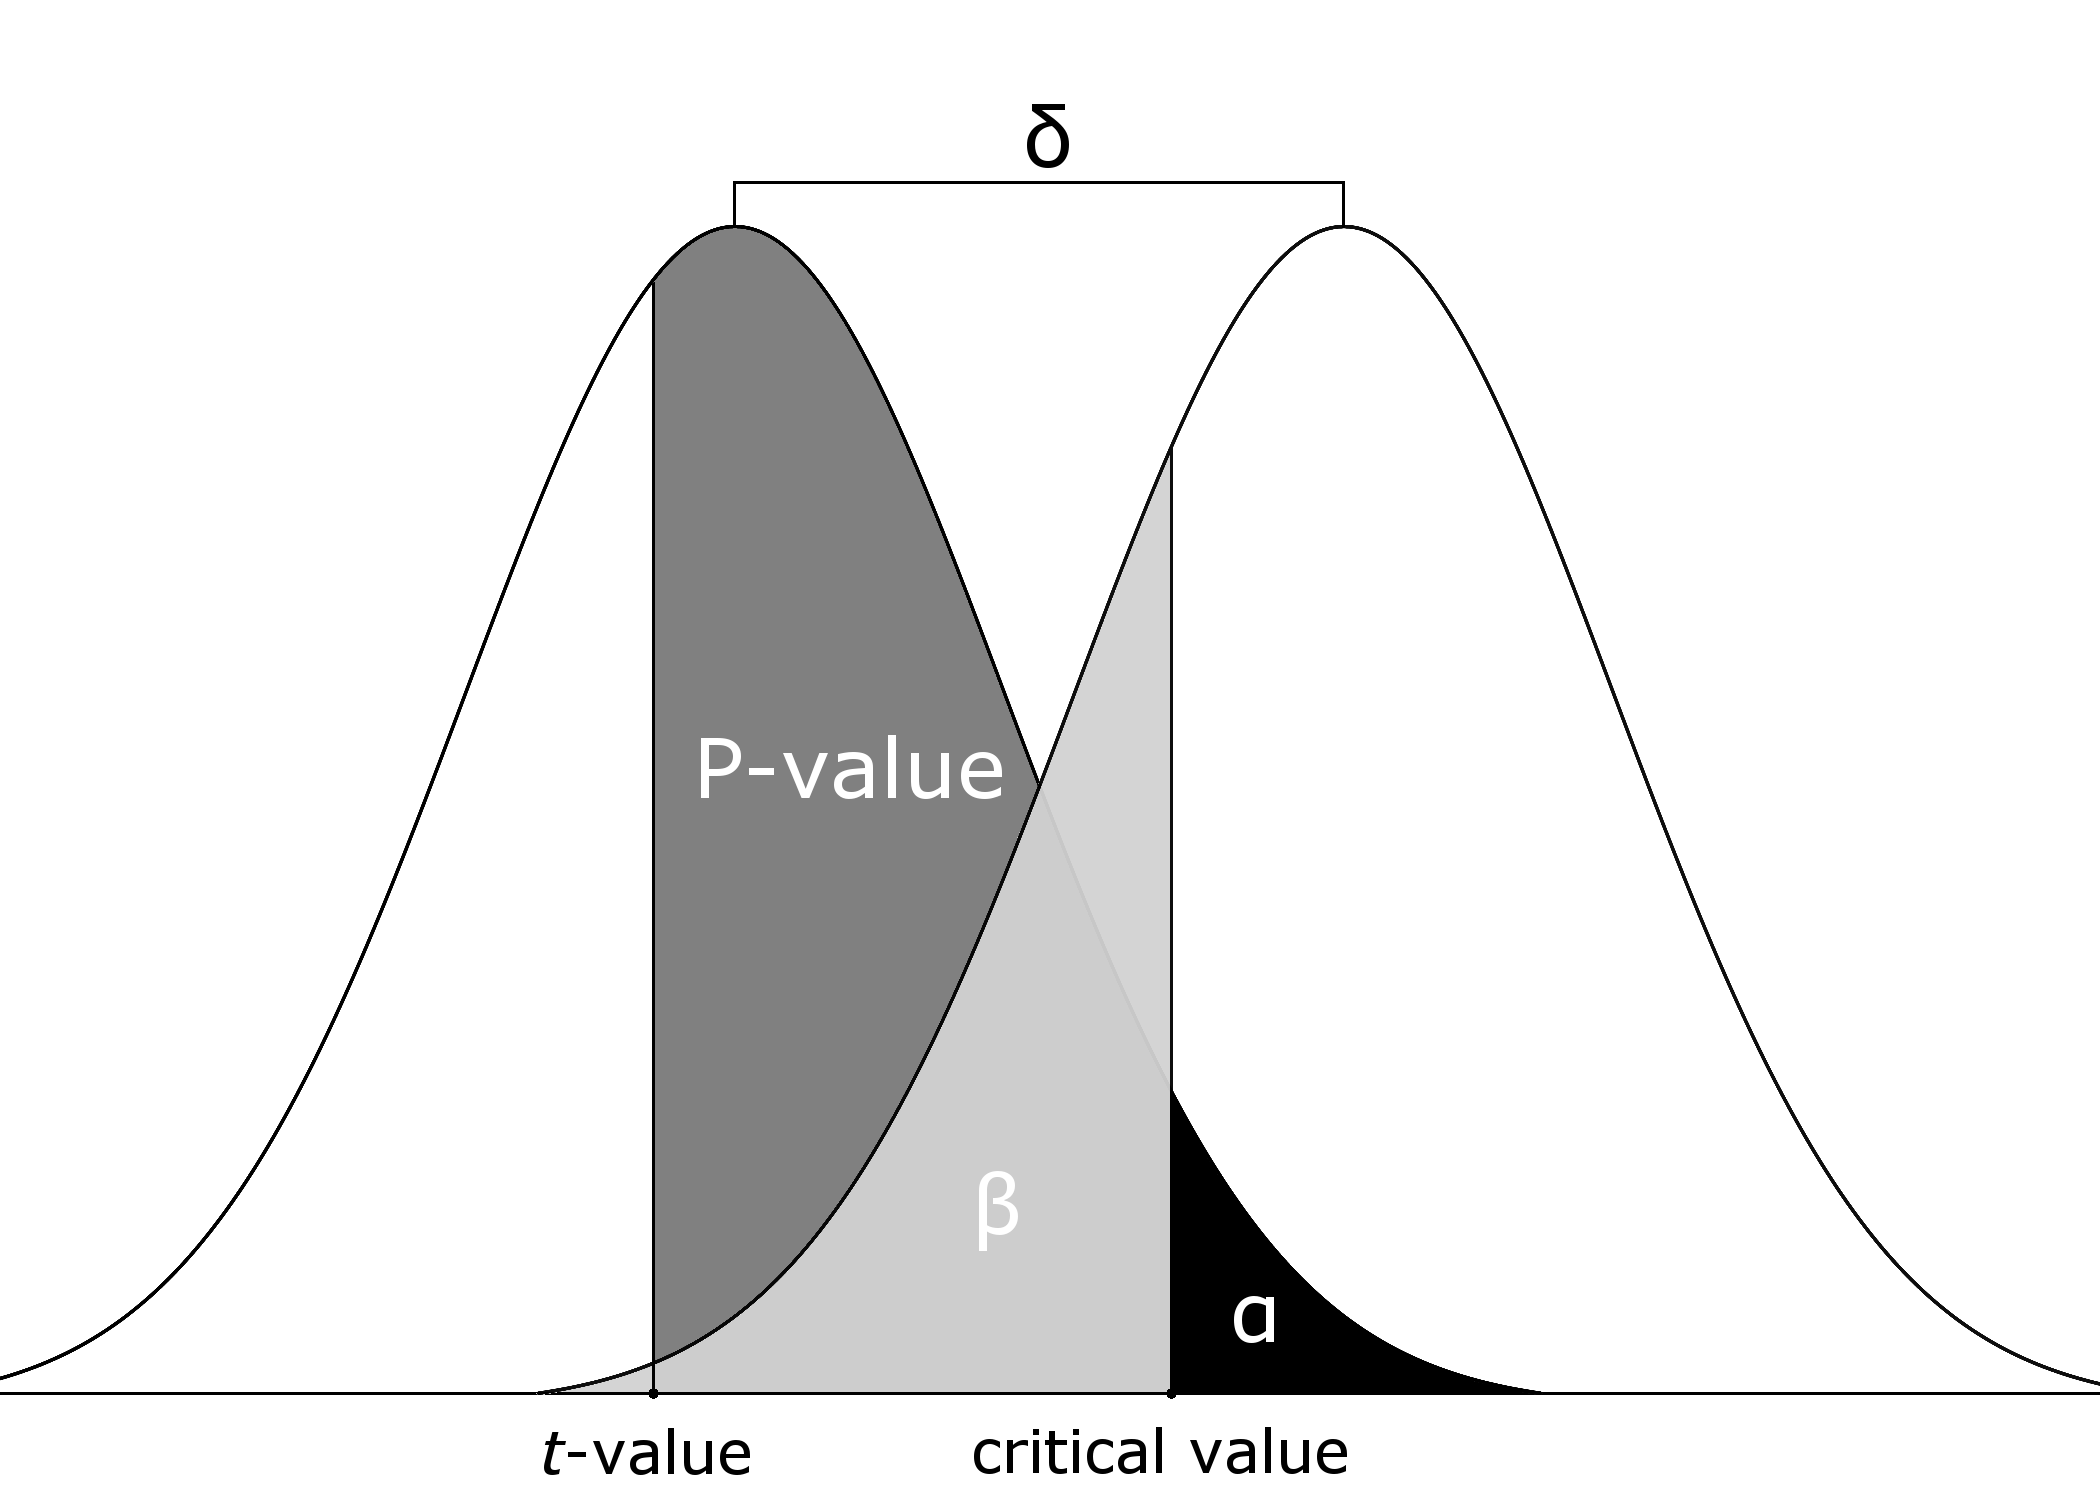
\includegraphics[width=1\linewidth]{assets/figures/tgtbf-appendix_a} 

}

\caption{Visual aid for simulating one nonsignificant test result. The critical value from $H_0$ (left distribution) was used to determine $\beta$ under $H_1$ (right distribution). A value between 0 and $\beta$ was drawn, $t$-value computed, and $p$-value under $H_0$ determined.}\label{fig:appendix5a}
\end{figure}

We repeated the procedure to simulate a false negative \(p\)-value \(k\)
times and used the resulting \(p\)-values to compute the Fisher test.
Before computing the Fisher test statistic, the nonsignificant
\(p\)-values were transformed (see Equation \eqref{eq:pistar}).
Subsequently, we computed the Fisher test statistic and the accompanying
\(p\)-value according to Equation \eqref{eq:fishertest}.

\chapter{Effect computation}\label{effect-computation}

The \(t\), \(F\), and \(r\)-values were all transformed into the effect
size \(\eta^2\), which is the explained variance for that test result
and ranges between 0 and 1, for comparing observed to expected effect
size distributions. For \(r\)-values, this only requires taking the
square (i.e., \(r^2\)). \(F\) and \(t\)-values were converted to effect
sizes by

\begin{equation}
\eta^2=\frac{\frac{F\times df_1}{df_2}}{\frac{F\times df_1}{df_2}+1}
\label{eq:b1}
\end{equation}

where \(F=t^2\) and \(df_1=1\) for \(t\)-values. Adjusted effect sizes,
which correct for positive bias due to sample size, were computed as

\begin{equation}
\eta^2_{adj}=\frac{\frac{F\times df_1}{df_2}-\frac{df_1}{df_2}}{\frac{F\times df_1}{df_2}+1}
\label{eq:b2}
\end{equation}

which shows that when \(F=1\) the adjusted effect size is zero. For
\(r\)-values the adjusted effect sizes were computed as (Ivarsson et al.
\protect\hyperlink{ref-doi:10.1016ux2fj.psychsport.2012.07.007}{2013})

\begin{equation}
\eta^2_{adj}=\eta^2-([1-\eta^2]\times\frac{v}{N-v-1})
\label{eq:b3}
\end{equation}

where \(v\) is the number of predictors. It was assumed that reported
correlations concern simple bivariate correlations and concern only one
predictor (i.e., \(v=1\)). This reduces the previous formula to

\begin{equation}
\eta^2_{adj}=\eta^2-\frac{1-\eta^2}{df}
\label{eq:b4}
\end{equation}

where \(df=N-2\).

\chapter{\texorpdfstring{Example of \texttt{statcheck} report for
PubPeer}{Example of statcheck report for PubPeer}}\label{example-of-statcheck-report-for-pubpeer}

\begin{quote}
The HTML version of this article was scanned on 5 August 2016 for
statistical results (\(t\), \(r\), \(F\), \(\chi^2\), and \(Z\) values)
reported in APA format (for specifics, see Nuijten, Hartgerink, et al.
\protect\hyperlink{ref-doi:10.3758ux2fs13428-015-0664-2}{2015}). An
automatically generated report follows.
\end{quote}

\begin{quote}
The scan detected 5 statistical results in APA format, of which 3
contained potentially incorrect statistical results, of which 1 may
change statistical significance (\(\alpha\)=0.05). Potential one-tailed
results were taken into account when \enquote{one-sided},
\enquote{one-tailed}, or \enquote{directional} occurred in the text. The
errors that may change statistical significance were reported as:
\end{quote}

\begin{quote}
\(t(67)=-0.436, p<0.001\) (recalculated \(p\)-value: 0.66424)
\end{quote}

\begin{quote}
The errors that may affect the computed \(p\)-value (but not the
statistical significance) were reported as:
\end{quote}

\begin{quote}
\(F(1,126)=2.1, p>0.90\) (recalculated \(p\)-value: 0.14978)
\end{quote}

\begin{quote}
\(t(67)=-1.02, p=0.35\) (recalculated \(p\)-value: 0.31140)
\end{quote}

\begin{quote}
Note that these are not definitive results and require manual inspection
to definitively assess whether results are erroneous.
\end{quote}

\chapter*{Bibliography}\label{bibliography}
\addcontentsline{toc}{chapter}{Bibliography}

\hypertarget{refs}{}
\hypertarget{ref-Aberson2010-xa}{}
Aberson, Christopher L. 2010. ``What is power? Why is power important?''
In \emph{Applied power analysis for the behavioral sciences}, edited by
Christopher L Aberson. New York, NY: Routledge.

\hypertarget{ref-doi:10.1371ux2fjournal.pone.0182651}{}
Aczel, Balazs, Bence Palfi, and Barnabas Szaszi. 2017. ``Estimating the
Evidential Value of Significant Results in Psychological Science.''
Edited by Jelte M. Wicherts. \emph{PLOS ONE} 12 (8). Public Library of
Science (PLoS): e0182651.
doi:\href{https://doi.org/10.1371/journal.pone.0182651}{10.1371/journal.pone.0182651}.

\hypertarget{ref-isbn:0471360937}{}
Agresti, Alan. 2003. \emph{Categorical Data Analysis}. Vol. 482. London,
United Kingdom: John Wiley \& Sons.
\url{https://mathdept.iut.ac.ir/sites/mathdept.iut.ac.ir/files/AGRESTI.PDF}.

\hypertarget{ref-doi:10.1186ux2f1471-2288-3-18}{}
Akhtar-Danesh, Noori, and Mahshid Dehghan-Kooshkghazi. 2003. ``How Does
Correlation Structure Differ Between Real and Fabricated Data-Sets?''
\emph{BMC Medical Research Methodology} 3 (1). Springer Nature.
doi:\href{https://doi.org/10.1186/1471-2288-3-18}{10.1186/1471-2288-3-18}.

\hypertarget{ref-doi:10.1080ux2f08989621.2013.822249}{}
Allen, Mary, and Robin Dowell. 2013. ``Retrospective Reflections of a
Whistleblower: Opinions on Misconduct Responses.'' \emph{Accountability
in Research} 20 (5-6): 339--48.
doi:\href{https://doi.org/10.1080/08989621.2013.822249}{10.1080/08989621.2013.822249}.

\hypertarget{ref-American_Psychological_Association1983-yf}{}
American Psychological Association. 1983. \emph{Publication manual of
the American Psychological Association}. 3rd ed. Washington, DC:
American Psychological Association.

\hypertarget{ref-American_Psychological_Association2001-uw}{}
---------. 2001. \emph{Publication manual of the American Psychological
Association}. 5th ed. Washington, DC: American Psychological
Association.

\hypertarget{ref-apa2010}{}
---------. 2010a. ``Ethical Principles of Psychologists and Code of
Conduct.'' \url{http://www.apa.org/ethics/code/principles.pdf}.
\url{http://www.apa.org/ethics/code/principles.pdf}.

\hypertarget{ref-isbn:9781433805615}{}
---------. 2010b. \emph{Publication Manual of the American Psychological
Association}. 6th ed. Washington, DC: American Psychological
Association.

\hypertarget{ref-doi:10.7287ux2fpeerj.preprints.2400v1}{}
Anaya, Jordan. 2016. ``The Grimmer Test: A Method for Testing the
Validity of Reported Measures of Variability.'' \emph{PeerJ Preprints} 4
(August): e2400v1.
doi:\href{https://doi.org/10.7287/peerj.preprints.2400v1}{10.7287/peerj.preprints.2400v1}.

\hypertarget{ref-doi:10.1126ux2fscience.aad9163}{}
Anderson, C. J., t pan Bahnik, M. Barnett-Cowan, F. A. Bosco, J.
Chandler, C. R. Chartier, F. Cheung, et al. 2016. ``Response to Comment
on `Estimating the Reproducibility of Psychological Science'.''
\emph{Science} 351 (6277). American Association for the Advancement of
Science (AAAS): 1037--7.
doi:\href{https://doi.org/10.1126/science.aad9163}{10.1126/science.aad9163}.

\hypertarget{ref-doi:10.1097ux2fACM.0b013e31812f764c}{}
Anderson, Melissa S, Aaron S Horn, Kelly R Risbey, Emily A Ronning,
Raymond De Vries, and Brian C Martinson. 2007. ``What Do Mentoring and
Training in the Responsible Conduct of Research Have to Do with
Scientists' Misbehavior? Findings from a National Survey of NIH-funded
Scientists.'' \emph{Academic Medicine} 82 (9): 853.
doi:\href{https://doi.org/10.1097/ACM.0b013e31812f764c}{10.1097/ACM.0b013e31812f764c}.

\hypertarget{ref-doi:10.1525ux2fjer.2007.2.4.3}{}
Anderson, Melissa S, Brian C Martinson, and Raymond De Vries. 2007.
``Normative Dissonance in Science: Results from a National Survey of
U.s. Scientists.'' \emph{Journal of Empirical Research on Human Research
Ethics} 2 (4): 3--14.
doi:\href{https://doi.org/10.1525/jer.2007.2.4.3}{10.1525/jer.2007.2.4.3}.

\hypertarget{ref-doi:10.1353ux2fjhe.0.0095}{}
Anderson, Melissa S, Emily A Ronning, Raymond Devries, and Brian C
Martinson. 2010. ``Extending the Mertonian Norms: Scientists'
Subscription to Norms of Research.'' \emph{The Journal of Higher
Education} 81 (3): 366--93.
doi:\href{https://doi.org/10.1353/jhe.0.0095}{10.1353/jhe.0.0095}.

\hypertarget{ref-foerster-complaint}{}
Anonymous. 2012. ``Suspicion of scientific misconduct by Dr. Jens
Foerster.''
\url{http://wayback.archive.org/web/20170511084213/https://retractionwatch.files.wordpress.com/2014/04/report_foerster.pdf}.

\hypertarget{ref-doi:10.2307ux2f2343787}{}
Armitage, P., C. K. McPherson, and B. C. Rowe. 1969. ``Repeated
Significance Tests on Accumulating Data.'' \emph{Journal of the Royal
Statistical Society. Series A (General)} 132 (2). JSTOR: 235.
doi:\href{https://doi.org/10.2307/2343787}{10.2307/2343787}.

\hypertarget{ref-doi:10.1002ux2fper.1919}{}
Asendorpf, Jens B., Mark Conner, Filip De Fruyt, Jan De Houwer, Jaap J.
A. Denissen, Klaus Fiedler, Susann Fiedler, et al. 2013.
``Recommendations for Increasing Replicability in Psychology.''
\emph{European Journal of Personality} 27 (2). Wiley: 108--19.
doi:\href{https://doi.org/10.1002/per.1919}{10.1002/per.1919}.

\hypertarget{ref-doi:10.1016ux2f0197-24569190037-M}{}
Bailey, Kent R. 1991. ``Detecting Fabrication of Data in a Multicenter
Collaborative Animal Study.'' \emph{Controlled Clinical Trials} 12 (6).
Elsevier BV: 741--52.
doi:\href{https://doi.org/10.1016/0197-2456(91)90037-m}{10.1016/0197-2456(91)90037-m}.

\hypertarget{ref-doi:10.1037ux2fh0020412}{}
Bakan, David. 1966. ``The Test of Significance in Psychological
Research.'' \emph{Psychological Bulletin} 66 (6). American Psychological
Association (APA): 423--37.
doi:\href{https://doi.org/10.1037/h0020412}{10.1037/h0020412}.

\hypertarget{ref-doi:10.1038ux2f533452a}{}
Baker, Monya. 2016. ``1,500 Scientists Lift the Lid on
Reproducibility.'' \emph{Nature} 533 (7604). Springer Nature: 452--54.
doi:\href{https://doi.org/10.1038/533452a}{10.1038/533452a}.

\hypertarget{ref-doi:10.3758ux2fs13428-011-0089-5}{}
Bakker, Marjan, and Jelte M Wicherts. 2011. ``The (Mis)reporting of
Statistical Results in Psychology Journals.'' \emph{Behavior Research
Methods} 43 (3): 666--78.
doi:\href{https://doi.org/10.3758/s13428-011-0089-5}{10.3758/s13428-011-0089-5}.

\hypertarget{ref-doi:10.1037ux2fmet0000014}{}
Bakker, Marjan, and Jelte M. Wicherts. 2014. ``Outlier Removal, Sum
Scores, and the Inflation of the Type I Error Rate in Independent
Samples T Tests: The Power of Alternatives and Recommendations.''
\emph{Psychological Methods} 19 (3). American Psychological Association
(APA): 409--27.
doi:\href{https://doi.org/10.1037/met0000014}{10.1037/met0000014}.

\hypertarget{ref-doi:10.1177ux2f1745691612459060}{}
Bakker, Marjan, Annette van Dijk, and Jelte M Wicherts. 2012. ``The
rules of the game called psychological science.'' \emph{Perspectives on
Psychological Science} 7 (6): 543--54.
doi:\href{https://doi.org/10.1177/1745691612459060}{10.1177/1745691612459060}.

\hypertarget{ref-doi:10.1177ux2f0956797616647519}{}
Bakker, Marjan, Chris H. J. Hartgerink, Jelte M. Wicherts, and Han L. J.
van der Maas. 2016. ``Researchers' Intuitions About Power in
Psychological Research.'' \emph{Psychological Science} 27 (8). SAGE
Publications: 1069--77.
doi:\href{https://doi.org/10.1177/0956797616647519}{10.1177/0956797616647519}.

\hypertarget{ref-isbn:9780226261454}{}
Baldwin, Melinda. 2015. \emph{Making Nature: The History of a Scientific
Journal}. University of Chicago Press.

\hypertarget{ref-isbn:9781400851911}{}
Baldwin, Peter. 2014. \emph{The Copyright Wars: Three Centuries of
Trans-Atlantic Battle}. Princeton University Press.

\hypertarget{ref-doi:10.1515ux2f9783110508420-010}{}
Bauer, Johannes, and Jochen Gross. 2011. ``Difficulties Detecting Fraud?
The Use of Benford's Law on Regression Tables.'' Edited by AndreasEditor
Diekmann. \emph{Methodological Artefacts, Data Manipulation and Fraud in
Economics and Social Science}, January. De Gruyter.
doi:\href{https://doi.org/10.1515/9783110508420-010}{10.1515/9783110508420-010}.

\hypertarget{ref-doi:10.1038ux2f483531a}{}
Begley, C. Glenn, and Lee M. Ellis. 2012. ``Raise Standards for
Preclinical Cancer Research.'' \emph{Nature} 483 (7391). Springer
Nature: 531--33.
doi:\href{https://doi.org/10.1038/483531a}{10.1038/483531a}.

\hypertarget{ref-doi:10.1017ux2fcbo9780511807862.002}{}
Bem, Daryl J. 2000. ``Writing an Empirical Article.'' Edited by Robert
J. Sternberg. Cambridge University Press, 3--16.
doi:\href{https://doi.org/10.1017/cbo9780511807862.002}{10.1017/cbo9780511807862.002}.

\hypertarget{ref-doi:10.2307ux2f984802}{}
Benford, Frank. 1938. ``The Law of Anomalous Numbers.''
\emph{Proceedings of the American Philosophical Society} 78 (4).
American Philosophical Society: 551--72.
\url{http://www.jstor.org/stable/984802}.

\hypertarget{ref-doi:10.1093ux2fbiostatisticsux2fkxt032}{}
Benjamini, Y., and Y. Hechtlinger. 2013. ``Discussion: An Estimate of
the Science-Wise False Discovery Rate and Applications to Top Medical
Journals by Jager and Leek.'' \emph{Biostatistics} 15 (1). Oxford
University Press (OUP): 13--16.
doi:\href{https://doi.org/10.1093/biostatistics/kxt032}{10.1093/biostatistics/kxt032}.

\hypertarget{ref-doi:10.1126ux2fscience.aaq0167}{}
Berg, Jeremy. 2017. ``Preprint Ecosystems.'' \emph{Science} 357 (6358).
American Association for the Advancement of Science (AAAS): 1331--1.
doi:\href{https://doi.org/10.1126/science.aaq0167}{10.1126/science.aaq0167}.

\hypertarget{ref-doi:10.1214ux2f11-ps175}{}
Berger, Arno, and Theodore P. Hill. 2011. ``A Basic Theory of Benford's
Law.'' \emph{Probability Surveys} 8 (0). Institute of Mathematical
Statistics: 1--126.
doi:\href{https://doi.org/10.1214/11-ps175}{10.1214/11-ps175}.

\hypertarget{ref-doi:10.1128ux2fmbio.00809-16}{}
Bik, Elisabeth M., Arturo Casadevall, and Ferric C. Fang. 2016a. ``The
Prevalence of Inappropriate Image Duplication in Biomedical Research
Publications.'' \emph{mBio} 7 (3). American Society for Microbiology:
e00809--16.
doi:\href{https://doi.org/10.1128/mbio.00809-16}{10.1128/mbio.00809-16}.

\hypertarget{ref-doi:10.1128ux2fmBio.00809-16}{}
---------. 2016b. ``The Prevalence of Inappropriate Image Duplication in
Biomedical Research Publications.'' \emph{mBio} 7 (3). American Society
for Microbiology: e00809--16.
doi:\href{https://doi.org/10.1128/mbio.00809-16}{10.1128/mbio.00809-16}.

\hypertarget{ref-doi:10.7287ux2fpeerj.preprints.1266v1}{}
Bishop, Dorothy V, and Paul A Thompson. 2015. ``Problems in Using
Text-Mining and P-Curve Analysis to Detect Rate of P-Hacking.''
\emph{PeerJ PrePrints} 3 (July): e1550.
doi:\href{https://doi.org/10.7287/peerj.preprints.1266v1}{10.7287/peerj.preprints.1266v1}.

\hypertarget{ref-doi:10.7717ux2fpeerj.1715}{}
Bishop, Dorothy V.M., and Paul A. Thompson. 2016. ``Problems in
Usingp-Curve Analysis and Text-Mining to Detect Rate Ofp-Hacking and
Evidential Value.'' \emph{PeerJ} 4 (February). PeerJ: e1715.
doi:\href{https://doi.org/10.7717/peerj.1715}{10.7717/peerj.1715}.

\hypertarget{ref-doi:10.1038ux2f527413f}{}
Bloudoff-Indelicato, Mollie. 2015. ``Text-Mining Block Prompts Online
Response.'' \emph{Nature} 527 (7579). Springer Nature: 413--13.
doi:\href{https://doi.org/10.1038/527413f}{10.1038/527413f}.

\hypertarget{ref-doi:10.1126ux2fscience.aaf5664}{}
Bohannon, John. 2016a. ``Who's Downloading Pirated Papers? Everyone.''
\emph{Science}.
doi:\href{https://doi.org/10.1126/science.aaf5664}{10.1126/science.aaf5664}.

\hypertarget{ref-doi:10.1126ux2fscience.352.6285.508}{}
---------. 2016b. ``Who's Downloading Pirated Papers? Everyone.''
\emph{Science} 352 (6285). American Association for the Advancement of
Science (AAAS): 508--12.
doi:\href{https://doi.org/10.1126/science.352.6285.508}{10.1126/science.352.6285.508}.

\hypertarget{ref-doi:10.1016ux2fj.jclinepi.2019.03.001}{}
Bolland, Mark J., Greg D. Gamble, Alison Avenell, and Andrew Grey. 2019.
``Rounding, but Not Randomization Method, Non-Normality, or Correlation,
Affected Baseline P-Value Distributions in Randomized Trials.''
\emph{Journal of Clinical Epidemiology} 110 (June). Elsevier BV: 50--62.
doi:\href{https://doi.org/10.1016/j.jclinepi.2019.03.001}{10.1016/j.jclinepi.2019.03.001}.

\hypertarget{ref-isbn:9781119964377}{}
Borenstein, Michael, Larry V. Hedges, Julian P. T. Higgins, and Hannah
R. Rothstein. 2011. \emph{Introduction to Meta-Analysis}. Wiley.

\hypertarget{ref-doi:10.1007ux2fs11948-015-9680-y}{}
Bornemann-Cimenti, Helmar, Istvan S Szilagyi, and Andreas
Sandner-Kiesling. 2015. ``Perpetuation of Retracted Publications Using
the Example of the Scott S. Reuben Case: Incidences, Reasons and
Possible Improvements.'' \emph{Science and Engineering Ethics},
7\textasciitilde{}jul.
doi:\href{https://doi.org/10.1007/s11948-015-9680-y}{10.1007/s11948-015-9680-y}.

\hypertarget{ref-doi:10.1007ux2fs11192-007-1950-2}{}
Bornmann, Lutz, Irina Nast, and Hans-Dieter Daniel. 2008. ``Do Editors
and Referees Look for Signs of Scientific Misconduct When Reviewing
Manuscripts? A Quantitative Content Analysis of Studies That Examined
Review Criteria and Reasons for Accepting and Rejecting Manuscripts for
Publication.'' \emph{Scientometrics} 77 (3). Springer Netherlands:
415--32.
doi:\href{https://doi.org/10.1007/s11192-007-1950-2}{10.1007/s11192-007-1950-2}.

\hypertarget{ref-doi:10.1038ux2fnpre.2007.39.1}{}
Bradley, Jean-Claude. 2007. ``Open Notebook Science Using Blogs and
Wikis.'' \emph{Nature Precedings}, June. Springer Nature.
doi:\href{https://doi.org/10.1038/npre.2007.39.1}{10.1038/npre.2007.39.1}.

\hypertarget{ref-doi:10.3389ux2ffnhum.2018.00037}{}
Brembs, Björn. 2018. ``Prestigious Science Journals Struggle to Reach
Even Average Reliability.'' \emph{Frontiers in Human Neuroscience} 12
(February). Frontiers Media SA.
doi:\href{https://doi.org/10.3389/fnhum.2018.00037}{10.3389/fnhum.2018.00037}.

\hypertarget{ref-isbn:9781786635471}{}
Bridle, James. 2018. \emph{New Dark Age: Technology and the End of the
Future}. Verso.

\hypertarget{ref-isbn:9780671447694}{}
Broad, William, and Nicholas Wade. 1983. \emph{Betrayers of the Truth}.
New York, NY: Simon; Schuster.

\hypertarget{ref-lg-irreg}{}
Broockman, David, Joshua Kalla, and Peter Aronow. 2015. ``Irregularities
in LaCour (2014).''
\url{https://wayback.archive.org/web/20180823093137/http://stanford.edu/~dbroock/broockman_kalla_aronow_lg_irregularities.pdf}.

\hypertarget{ref-doi:10.1177ux2f1948550616673876}{}
Brown, Nicholas J. L., and James A. J. Heathers. 2016. ``The GRIM
Test.'' \emph{Social Psychological and Personality Science} 8 (4). SAGE
Publications: 363--69.
doi:\href{https://doi.org/10.1177/1948550616673876}{10.1177/1948550616673876}.

\hypertarget{ref-doi:10.1371ux2fjournal.pone.0149144}{}
Bruns, Stephan B., and John P. A. Ioannidis. 2016. ``P-Curve and
P-Hacking in Observational Research.'' \emph{PLOS ONE} 11 (2). Public
Library of Science: 1--13.
doi:\href{https://doi.org/10.1371/journal.pone.0149144}{10.1371/journal.pone.0149144}.

\hypertarget{ref-Burns2009}{}
Burns, Bruce D. 2009. ``Sensitivity to statistical regularities : People
(largely) follow Benford's law.'' In \emph{Proceedings of the Thirty
First Annual Conference of the Cognitive Science Society}. Austin, TX:
Cognitive Science Society.
\url{http://wayback.archive.org/web/20170619175106/http://csjarchive.cogsci.rpi.edu/Proceedings/2009/papers/637/paper637.pdf}.

\hypertarget{ref-buyse1999}{}
Buyse, M, S L George, S Evans, N L Geller, J Ranstam, B Scherrer, E
Lesaffre, et al. 1999. ``The Role of Biostatistics in the Prevention,
Detection and Treatment of Fraud in Clinical Trials.'' \emph{Statistics
in Medicine} 18 (24): 3435--51.
doi:\href{https://doi.org/10.1002/(SICI)1097-0258(19991230)18:24\%3C3435::AID-SIM365\%3E3.0.CO;2-O}{10.1002/(SICI)1097-0258(19991230)18:24\textless{}3435::AID-SIM365\textgreater{}3.0.CO;2-O}.

\hypertarget{ref-doi:10.1126ux2fscience.aaf0918}{}
Camerer, C. F., A. Dreber, E. Forsell, T.-H. Ho, J. Huber, M.
Johannesson, M. Kirchler, et al. 2016. ``Evaluating Replicability of
Laboratory Experiments in Economics.'' \emph{Science} 351 (6280).
American Association for the Advancement of Science (AAAS): 1433--6.
doi:\href{https://doi.org/10.1126/science.aaf0918}{10.1126/science.aaf0918}.

\hypertarget{ref-dokieli}{}
Capadisli, Sarven, Amy Guy, Ruben Verborgh, Christoph Lange, Soeren
Auer, and Tim Berners-Lee. 2017. ``Decentralised Authoring, Annotations
and Notifications for a Read-Write Web with Dokieli.''
\url{https://wayback.archive.org/web/20180807191810/http://csarven.ca/dokieli-rww}.

\hypertarget{ref-doi:10.1111ux2fj.1365-2044.2012.07128.x}{}
Carlisle, J. B. 2012. ``The Analysis of 168 Randomised Controlled Trials
to Test Data Integrity.'' \emph{Anaesthesia} 67 (5): 521--37.
doi:\href{https://doi.org/10.1111/j.1365-2044.2012.07128.x}{10.1111/j.1365-2044.2012.07128.x}.

\hypertarget{ref-doi:10.1111ux2fanae.13938}{}
---------. 2017a. ``Data Fabrication and Other Reasons for Non-Random
Sampling in 5087 Randomised, Controlled Trials in Anaesthetic and
General Medical Journals.'' \emph{Anaesthesia}, June. Wiley-Blackwell.
doi:\href{https://doi.org/10.1111/anae.13938}{10.1111/anae.13938}.

\hypertarget{ref-doi:10.1111ux2fanae.14148}{}
---------. 2017b. ``Seeking and Reporting Apparent Research Misconduct:
Errors and Integrity - a Reply.'' \emph{Anaesthesia} 73 (1). Wiley:
126--28.
doi:\href{https://doi.org/10.1111/anae.14148}{10.1111/anae.14148}.

\hypertarget{ref-doi:10.1111ux2fanae.13650}{}
Carlisle, J. B., and J. A. Loadsman. 2016. ``Evidence for Non-Random
Sampling in Randomised, Controlled Trials by Yuhji Saitoh.''
\emph{Anaesthesia} 72 (1). Wiley: 17--27.
doi:\href{https://doi.org/10.1111/anae.13650}{10.1111/anae.13650}.

\hypertarget{ref-doi:10.1111ux2fanae.13126}{}
Carlisle, J. B., F. Dexter, J. J. Pandit, S. L. Shafer, and S. M.
Yentis. 2015. ``Calculating the Probability of Random Sampling for
Continuous Variables in Submitted or Published Randomised Controlled
Trials.'' \emph{Anaesthesia} 70 (7): 848--58.
doi:\href{https://doi.org/10.1111/anae.13126}{10.1111/anae.13126}.

\hypertarget{ref-isbn:9780534243128}{}
Casella, George, and Roger L. Berger. 2001. \emph{Statistical
Inference}. Cengage Learning.

\hypertarget{ref-doi:10.1109ux2fglocom.2012.6503613}{}
Cavdar, Derya, and Fatih Alagoz. 2012. ``A Survey of Research on
Greening Data Centers.'' \emph{2012 IEEE Global Communications
Conference (GLOBECOM)}, December. IEEE.
doi:\href{https://doi.org/10.1109/glocom.2012.6503613}{10.1109/glocom.2012.6503613}.

\hypertarget{ref-Chamberlain2015-tg}{}
Chamberlain, Scott, Carl Boettiger, and Karthik Ram. 2015. ``Rplos:
Interface to the Search 'API' for 'PLoS' Journals.''
\url{http://CRAN.R-project.org/package=rplos}.

\hypertarget{ref-doi:10.1111ux2fadd.12728}{}
Chambers, Christopher D. 2015. ``Ten Reasons Why Journals Must Review
Manuscripts Before Results Are Known.'' \emph{Addiction} 110 (1):
10--11. doi:\href{https://doi.org/10.1111/add.12728}{10.1111/add.12728}.

\hypertarget{ref-doi:10.1016ux2fj.cortex.2012.12.016}{}
Chambers, Christopher D. 2013. ``Registered Reports: A New Publishing
Initiative at~Cortex.'' \emph{Cortex} 49 (3). Elsevier BV: 609--10.
doi:\href{https://doi.org/10.1016/j.cortex.2012.12.016}{10.1016/j.cortex.2012.12.016}.

\hypertarget{ref-doi:10.1177ux2f1745691616664694}{}
Cheung, I., L. Campbell, E. P. LeBel, R. A. Ackerman, B. Aykutoğlu, Š.
Bahník, J. D. Bowen, et al. 2016. ``Registered Replication Report.''
\emph{Perspectives on Psychological Science} 11 (5). SAGE Publications:
750--64.
doi:\href{https://doi.org/10.1177/1745691616664694}{10.1177/1745691616664694}.

\hypertarget{ref-doi:10.2307ux2f27643897}{}
Cho, Wendy K. Tam, and Brian J. Gaines. 2007. ``Breaking the (Benford)
Law: Statistical Fraud Detection in Campaign Finance.'' \emph{The
American Statistician} 61 (3). {[}American Statistical Association,
Taylor \& Francis, Ltd.{]}: 218--23.
\url{http://www.jstor.org/stable/27643897}.

\hypertarget{ref-doi:10.1146ux2fannurev.psych.55.090902.142015}{}
Cialdini, Robert B., and Noah J. Goldstein. 2004. ``Social Influence:
Compliance and Conformity.'' \emph{Annual Review of Psychology} 55 (1).
Annual Reviews: 591--621.
doi:\href{https://doi.org/10.1146/annurev.psych.55.090902.142015}{10.1146/annurev.psych.55.090902.142015}.

\hypertarget{ref-doi:10.1186ux2f2041-1480-5-28}{}
Clark, Tim, Paolo N Ciccarese, and Carole A Goble. 2014.
``Micropublications: A Semantic Model for Claims, Evidence, Arguments
and Annotations in Biomedical Communications.'' \emph{Journal of
Biomedical Semantics} 5 (1). Springer Nature: 28.
doi:\href{https://doi.org/10.1186/2041-1480-5-28}{10.1186/2041-1480-5-28}.

\hypertarget{ref-doi:10.1037ux2fh0045186}{}
Cohen, Jacob. 1962. ``The Statistical Power of Abnormal-Social
Psychological Research: A Review.'' \emph{The Journal of Abnormal and
Social Psychology} 65 (3). American Psychological Association (APA):
145--53. doi:\href{https://doi.org/10.1037/h0045186}{10.1037/h0045186}.

\hypertarget{ref-isbn:9780805802832}{}
---------. 1988. \emph{Statistical Power Analysis for the Behavioral
Sciences (2nd Edition)}. Routledge.

\hypertarget{ref-doi:10.1037ux2f0003-066X.49.12.997}{}
---------. 1994. ``The Earth Is Round (P \textless{} .05).''
\emph{American Psychologist} 49 (12): 997--1003.
doi:\href{https://doi.org/10.1037/0003-066X.49.12.997}{10.1037/0003-066X.49.12.997}.

\hypertarget{ref-doi:10.1038ux2f493147a}{}
Cressey, Daniel. 2013. ``'Rehab' Helps Errant Researchers Return to the
Lab.'' \emph{Nature News} 493 (7431): 147.
doi:\href{https://doi.org/10.1038/493147a}{10.1038/493147a}.

\hypertarget{ref-doi:10.1177ux2f0956797613504966}{}
Cumming, Geoff. 2013. ``The New Statistics.'' \emph{Psychological
Science} 25 (1). SAGE Publications: 7--29.
doi:\href{https://doi.org/10.1177/0956797613504966}{10.1177/0956797613504966}.

\hypertarget{ref-doi:10.1038ux2f520600a}{}
Cyranoski, David. 2015. ``Collateral Damage: How One Misconduct Case
Brought a Biology Institute to Its Knees.'' \emph{Nature} 520 (7549).
Springer Nature: 600--603.
doi:\href{https://doi.org/10.1038/520600a}{10.1038/520600a}.

\hypertarget{ref-isbn:9789023228912}{}
De Groot, A.D. 1994. \emph{Methodologie: Grondslagen van Onderzoek En
Denken in de Gedragswetenschappen {[}Methodology: Foundations of
Research and Thinking in the Behavioral Sciences{]}}. Assen, the
Netherlands: Van Gorcum.

\hypertarget{ref-doi:10.7717ux2fpeerj.733}{}
De Winter, Joost CF, and Dimitra Dodou. 2015. ``A Surge of P-Values
Between 0.041 and 0.049 in Recent Decades (but Negative Results Are
Increasing Rapidly Too).'' \emph{PeerJ} 3 (January). PeerJ: e733.
doi:\href{https://doi.org/10.7717/peerj.733}{10.7717/peerj.733}.

\hypertarget{ref-doi:10.1080ux2f02664760601004940}{}
Diekmann, Andreas. 2007. ``Not the First Digit! Using Benford's Law to
Detect Fraudulent Scientific Data.'' \emph{Journal of Applied
Statistics} 34 (3). Taylor \& Francis: 321--29.
doi:\href{https://doi.org/10.1080/02664760601004940}{10.1080/02664760601004940}.

\hypertarget{ref-doi:10.1103ux2fphysreve.95.022313}{}
Domenico, Manlio De, and Alex Arenas. 2017. ``Modeling Structure and
Resilience of the Dark Network.'' \emph{Physical Review E} 95 (2).
American Physical Society (APS).
doi:\href{https://doi.org/10.1103/physreve.95.022313}{10.1103/physreve.95.022313}.

\hypertarget{ref-durtschi2004effective}{}
Durtschi, Cindy, William Hillison, and Carl Pacini. 2004. ``The
Effective Use of Benford's Law to Assist in Detecting Fraud in
Accounting Data.'' \emph{Journal of Forensic Accounting} 5 (1): 17--34.

\hypertarget{ref-doi:10.1016ux2f0140-6736_91_90201-y}{}
Easterbrook, P.J, R Gopalan, J.A Berlin, and D.R Matthews. 1991.
``Publication Bias in Clinical Research.'' \emph{The Lancet} 337 (8746).
Elsevier BV: 867--72.
doi:\href{https://doi.org/10.1016/0140-6736(91)90201-y}{10.1016/0140-6736(91)90201-y}.

\hypertarget{ref-doi:10.1016ux2fj.jesp.2015.10.012}{}
Ebersole, Charles R., Olivia E. Atherton, Aimee L. Belanger, Hayley M.
Skulborstad, Jill M. Allen, Jonathan B. Banks, Erica Baranski, et al.
2016. ``Many Labs 3: Evaluating Participant Pool Quality Across the
Academic Semester via Replication.'' \emph{Journal of Experimental
Social Psychology} 67 (November). Elsevier BV: 68--82.
doi:\href{https://doi.org/10.1016/j.jesp.2015.10.012}{10.1016/j.jesp.2015.10.012}.

\hypertarget{ref-doi:10.1371ux2fjournal.pone.0085846}{}
Elia, Nadia, Elizabeth Wager, and Martin R. Tramèr. 2014. ``Fate of
Articles That Warranted Retraction Due to Ethical Concerns: A
Descriptive Cross-Sectional Study.'' Edited by K. BradEditor Wray.
\emph{PLoS ONE} 9 (1). Public Library of Science (PLoS): e85846.
doi:\href{https://doi.org/10.1371/journal.pone.0085846}{10.1371/journal.pone.0085846}.

\hypertarget{ref-ellemers}{}
Ellemers, Naomi. 2017. ``Ethisch klimaat op het werk: Op zoek naar het
nieuwe normaal {[}Ethical climate at work: Searching for the new
normal{]}.''
\url{https://wayback.archive.org/web/20180726070256/https://www.scoop-program.org/images/Tekst_Oratie_Naomi_Ellemers_9_februari_2017.pdf}.

\hypertarget{ref-statcheck}{}
Epskamp, Sacha, and Michèle B. Nuijten. 2016. \emph{Statcheck: Extract
Statistics from Articles and Recompute P Values}.
\url{https://CRAN.R-project.org/package=statcheck}.

\hypertarget{ref-doi:10.1371ux2fjournal.pone.0149794}{}
Etz, Alexander, and Joachim Vandekerckhove. 2016. ``A Bayesian
Perspective on the Reproducibility Project: Psychology.'' Edited by
DanieleEditor Marinazzo. \emph{PLOS ONE} 11 (2). Public Library of
Science (PLoS): e0149794.
doi:\href{https://doi.org/10.1371/journal.pone.0149794}{10.1371/journal.pone.0149794}.

\hypertarget{ref-doi:10.1371ux2fjournal.pone.0005738}{}
Fanelli, Daniele. 2009. ``How Many Scientists Fabricate and Falsify
Research? A Systematic Review and Meta-Analysis of Survey Data.''
\emph{PloS ONE} 4 (5): e5738.
doi:\href{https://doi.org/10.1371/journal.pone.0005738}{10.1371/journal.pone.0005738}.

\hypertarget{ref-doi:10.1007ux2fs11192-011-0494-7}{}
---------. 2011. ``Negative Results Are Disappearing from Most
Disciplines and Countries.'' \emph{Scientometrics} 90 (3). Springer
Nature: 891--904.
doi:\href{https://doi.org/10.1007/s11192-011-0494-7}{10.1007/s11192-011-0494-7}.

\hypertarget{ref-doi:10.1007ux2fs11948-018-0023-7}{}
Fanelli, Daniele, Rodrigo Costas, Ferric C. Fang, Arturo Casadevall, and
Elisabeth M. Bik. 2018. ``Testing Hypotheses on Risk Factors for
Scientific Misconduct via Matched-Control Analysis of Papers Containing
Problematic Image Duplications.'' \emph{Science and Engineering Ethics},
February. Springer Nature.
doi:\href{https://doi.org/10.1007/s11948-018-0023-7}{10.1007/s11948-018-0023-7}.

\hypertarget{ref-doi:10.1073ux2fpnas.1212247109}{}
Fang, Ferric C, R Grant Steen, and Arturo Casadevall. 2012. ``Misconduct
Accounts for the Majority of Retracted Scientific Publications.''
\emph{Proceedings of the National Academy of Sciences of the United
States of America} 109 (42): 17028--33.
doi:\href{https://doi.org/10.1073/pnas.1212247109}{10.1073/pnas.1212247109}.

\hypertarget{ref-doi:10.1016ux2fj.gendis.2015.02.006}{}
Fareed, Mohd, Malik Azeem Anwar, and Mohammad Afzal. 2015. ``Prevalence
and Gene Frequency of Color Vision Impairments Among Children of Six
Populations from North Indian Region.'' \emph{Genes \& Diseases} 2 (2).
Elsevier BV: 211--18.
doi:\href{https://doi.org/10.1016/j.gendis.2015.02.006}{10.1016/j.gendis.2015.02.006}.

\hypertarget{ref-doi:10.1037ux2fa0039405}{}
Ferguson, Christopher J. 2015. ```Everybody Knows Psychology Is Not a
Real Science': Public Perceptions of Psychology and How We Can Improve
Our Relationship with Policymakers, the Scientific Community, and the
General Public.'' \emph{American Psychologist} 70 (6). American
Psychological Association (APA): 527--42.
doi:\href{https://doi.org/10.1037/a0039405}{10.1037/a0039405}.

\hypertarget{ref-doi:10.1198ux2ftast.2009.0005}{}
Fewster, R. M. 2009. ``A Simple Explanation of Benford's Law.''
\emph{The American Statistician} 63 (1): 26--32.
doi:\href{https://doi.org/10.1198/tast.2009.0005}{10.1198/tast.2009.0005}.

\hypertarget{ref-doi:10.1177ux2f1745691612462587}{}
Fiedler, Klaus, Florian Kutzner, and Joachim I. Krueger. 2012. ``The
Long Way from Alpha-Error Control to Validity Proper.''
\emph{Perspectives on Psychological Science} 7 (6). SAGE Publications:
661--69.
doi:\href{https://doi.org/10.1177/1745691612462587}{10.1177/1745691612462587}.

\hypertarget{ref-Fisher1925-jl}{}
Fisher, Ronald Aylmer. 1925. \emph{Statistical methods for research
workers}. Edinburg, United Kingdom: Oliver Boyd.

\hypertarget{ref-isbn:9780226253251}{}
Fleck, Ludwig. 1984. \emph{Genesis and Development of a Scientific
Fact}. Chicago, IL: University of Chicago Press.

\hypertarget{ref-doi:10.1126ux2fscience.aao0185}{}
Fortunato, Santo, Carl T. Bergstrom, Katy Börner, James A. Evans, Dirk
Helbing, Staša Milojević, Alexander M. Petersen, et al. 2018. ``Science
of Science.'' \emph{Science} 359 (6379). American Association for the
Advancement of Science (AAAS): eaao0185.
doi:\href{https://doi.org/10.1126/science.aao0185}{10.1126/science.aao0185}.

\hypertarget{ref-doi:10.1371ux2fjournal.pone.0109019}{}
Fraley, R. Chris, and Simine Vazire. 2014. ``The N-Pact Factor:
Evaluating the Quality of Empirical Journals with Respect to Sample Size
and Statistical Power.'' Edited by Christos A.Editor Ouzounis.
\emph{PLoS ONE} 9 (10). Public Library of Science (PLoS): e109019.
doi:\href{https://doi.org/10.1371/journal.pone.0109019}{10.1371/journal.pone.0109019}.

\hypertarget{ref-doi:10.3758ux2fs13423-012-0227-9}{}
Francis, Gregory. 2012. ``Too Good to Be True: Publication Bias in Two
Prominent Studies from Experimental Psychology.'' \emph{Psychonomic
Bulletin \& Review} 19 (2). Springer Nature: 151--56.
doi:\href{https://doi.org/10.3758/s13423-012-0227-9}{10.3758/s13423-012-0227-9}.

\hypertarget{ref-doi:10.1126ux2fscience.1255484}{}
Franco, Annie, Neil Malhotra, and Gabor Simonovits. 2014. ``Publication
Bias in the Social Sciences: Unlocking the File Drawer.'' \emph{Science}
345 (6203): 1502--5.
doi:\href{https://doi.org/10.1126/science.1255484}{10.1126/science.1255484}.

\hypertarget{ref-doi:10.1177ux2f1948550615598377}{}
---------. 2016. ``Underreporting in Psychology Experiments: Evidence
from a Study Registry.'' \emph{Social Psychological and Personality
Science} 7 (1): 8--12.
doi:\href{https://doi.org/10.1177/1948550615598377}{10.1177/1948550615598377}.

\hypertarget{ref-doi:10.1186ux2f1471-2288-4-13}{}
García-Berthou, Emili, and Carles Alcaraz. 2004. ``Incongruence Between
Test Statistics and P Values in Medical Papers.'' \emph{BMC Medical
Research Methodology} 4 (1). Springer Nature.
doi:\href{https://doi.org/10.1186/1471-2288-4-13}{10.1186/1471-2288-4-13}.

\hypertarget{ref-doi:10.1001ux2fjama.295.1.90}{}
Garfield, Eugene. 2006. ``The History and Meaning of the Journal Impact
Factor.'' \emph{JAMA} 295 (1). American Medical Association (AMA): 90.
doi:\href{https://doi.org/10.1001/jama.295.1.90}{10.1001/jama.295.1.90}.

\hypertarget{ref-doi:10.1093ux2fbiostatisticsux2fkxt034}{}
Gelman, A., and K. O'Rourke. 2013. ``Discussion: Difficulties in Making
Inferences About Scientific Truth from Distributions of Published
P-Values.'' \emph{Biostatistics} 15 (1). Oxford University Press (OUP):
18--23.
doi:\href{https://doi.org/10.1093/biostatistics/kxt034}{10.1093/biostatistics/kxt034}.

\hypertarget{ref-gelman-forking}{}
Gelman, Andrew, and Eric Loken. 2013. ``The Garden of Forking Paths: Why
Multiple Comparisons Can Be a Problem, Even When There Is No `Fishing
Expedition' or `P-Hacking' and the Research Hypothesis Was Posited Ahead
of Time.''
\url{https://wayback.archive.org/web/20180712075516/http://www.stat.columbia.edu/~gelman/research/unpublished/p_hacking.pdf}.

\hypertarget{ref-doi:10.1177ux2f1532673x09350979}{}
Gerber, Alan S., Neil Malhotra, Conor M. Dowling, and David Doherty.
2010. ``Publication Bias in Two Political Behavior Literatures.''
\emph{American Politics Research} 38 (4). SAGE Publications: 591--613.
doi:\href{https://doi.org/10.1177/1532673x09350979}{10.1177/1532673x09350979}.

\hypertarget{ref-doi:10.1016ux2fj.paid.2016.06.069}{}
Gignac, Gilles E., and Eva T. Szodorai. 2016. ``Effect Size Guidelines
for Individual Differences Researchers.'' \emph{Personality and
Individual Differences} 102 (November). Elsevier BV: 74--78.
doi:\href{https://doi.org/10.1016/j.paid.2016.06.069}{10.1016/j.paid.2016.06.069}.

\hypertarget{ref-doi:10.1126ux2fscience.aad7243}{}
Gilbert, D. T., G. King, S. Pettigrew, and T. D. Wilson. 2016. ``Comment
on `Estimating the Reproducibility of Psychological Science'.''
\emph{Science} 351 (6277). American Association for the Advancement of
Science (AAAS): 1037--7.
doi:\href{https://doi.org/10.1126/science.aad7243}{10.1126/science.aad7243}.

\hypertarget{ref-doi:10.1177ux2f1745691612457576}{}
Giner-Sorolla, Roger. 2012. ``Science or Art? How Aesthetic Standards
Grease the Way Through the Publication Bottleneck but Undermine
Science.'' \emph{Perspectives on Psychological Science} 7 (6). SAGE
Publications: 562--71.
doi:\href{https://doi.org/10.1177/1745691612457576}{10.1177/1745691612457576}.

\hypertarget{ref-doi:10.1186ux2fs13104-015-1691-x}{}
Ginsel, Bastiaan, Abhinav Aggarwal, Wei Xuan, and Ian Harris. 2015.
``The Distribution of Probability Values in Medical Abstracts: An
Observational Study.'' \emph{BMC Research Notes} 8 (1). Springer Nature.
doi:\href{https://doi.org/10.1186/s13104-015-1691-x}{10.1186/s13104-015-1691-x}.

\hypertarget{ref-doi:10.1093ux2fbiostatisticsux2fkxt035}{}
Goodman, S. N. 2013. ``Discussion: An Estimate of the Science-Wise False
Discovery Rate and Application to the Top Medical Literature.''
\emph{Biostatistics} 15 (1). Oxford University Press (OUP): 23--27.
doi:\href{https://doi.org/10.1093/biostatistics/kxt035}{10.1093/biostatistics/kxt035}.

\hypertarget{ref-doi:10.1053ux2fj.seminhematol.2008.04.003}{}
Goodman, Steven. 2008. ``A Dirty Dozen: Twelve P-Value Misconceptions.''
\emph{Seminars in Hematology} 45 (3). Elsevier BV: 135--40.
doi:\href{https://doi.org/10.1053/j.seminhematol.2008.04.003}{10.1053/j.seminhematol.2008.04.003}.

\hypertarget{ref-doi:10.1037ux2fh0076157}{}
Greenwald, Anthony G. 1975. ``Consequences of Prejudice Against the Null
Hypothesis.'' \emph{Psychological Bulletin} 82 (1). American
Psychological Association (APA): 1--20.
doi:\href{https://doi.org/10.1037/h0076157}{10.1037/h0076157}.

\hypertarget{ref-doi:10.7287ux2fpeerj.preprints.27809v1}{}
Grossmann, Alexander, and Björn Brembs. 2019. ``Assessing the Size of
the Affordability Problem in Scholarly Publishing,'' June. PeerJ.
doi:\href{https://doi.org/10.7287/peerj.preprints.27809v1}{10.7287/peerj.preprints.27809v1}.

\hypertarget{ref-doi:10.3233ux2fisu-2010-0613}{}
Groth, Paul, Andrew Gibson, and Jan Velterop. 2010. ``The Anatomy of a
Nanopublication.'' \emph{Information Services \& Use} 30 (1-2). IOS
Press: 51--56.
doi:\href{https://doi.org/10.3233/isu-2010-0613}{10.3233/isu-2010-0613}.

\hypertarget{ref-Haldane1948-nm}{}
Haldane, J B S. 1948. ``The faking of genetical results.'' \emph{Eureka}
6: 21--28.
\url{http://wayback.archive.org/web/20170206144438/http://www.archim.org.uk/eureka/27/faking.html}.

\hypertarget{ref-doi:10.1148ux2fradiology.143.1.7063747}{}
Hanley, J A, and B J McNeil. 1982. ``The Meaning and Use of the Area
Under a Receiver Operating Characteristic (ROC) Curve.''
\emph{Radiology} 143 (1). Radiological Society of North America (RSNA):
29--36.
doi:\href{https://doi.org/10.1148/radiology.143.1.7063747}{10.1148/radiology.143.1.7063747}.

\hypertarget{ref-cogprints1646}{}
Harnad, Stevan. 2000. ``The Invisible Hand of Peer Review.''
\emph{Exploit Interactive}. \url{http://cogprints.org/1646/}.

\hypertarget{ref-doi:10.6084ux2fm9.figshare.928315.v2}{}
Hartgerink, Chris H. J. 2014. ``Poster: Low Threshold Open Science.''
figshare.
doi:\href{https://doi.org/10.6084/m9.figshare.928315.v2}{10.6084/m9.figshare.928315.v2}.

\hypertarget{ref-doi:10.15200ux2fwinn.144232.26366}{}
---------. 2015a. ``Do Not Trust Science Verify It.'' Authorea, Inc.
doi:\href{https://doi.org/10.15200/winn.144232.26366}{10.15200/winn.144232.26366}.

\hypertarget{ref-ons-elsevier}{}
---------. 2015b. ``Elsevier Stopped Me Doing My Research.''
\url{https://wayback.archive.org/web/20180814123817/http://onsnetwork.org/chartgerink/2015/11/16/elsevier-stopped-me-doing-my-research/}.

\hypertarget{ref-ons-wiley}{}
---------. 2016a. ``Wiley Also Stopped Me Doing My Research.''
\url{https://wayback.archive.org/web/20180814123807/http://onsnetwork.org/chartgerink/2016/02/23/wiley-also-stopped-my-doing-my-research/}.

\hypertarget{ref-doi:10.3390ux2fdata1030014}{}
---------. 2016b. ``688,112 Statistical Results: Content Mining
Psychology Articles for Statistical Test Results.'' \emph{Data} 1 (3).
MDPI AG: 14.
doi:\href{https://doi.org/10.3390/data1030014}{10.3390/data1030014}.

\hypertarget{ref-Hartgerink-dlib2017}{}
---------. 2017a. ``Developing the Potential of Data Extraction in
Scholarly Articles for Research Verification.'' \emph{D-Lib Magazine}.
\url{http://www.dlib.org/dlib/may17/05inbrief.html\#HARTGERINK}.

\hypertarget{ref-doi:10.7717ux2fpeerj.3068}{}
---------. 2017b. ``Reanalyzing Head et Al. (2015): Investigating the
Robustness of Widespread P-Hacking.'' \emph{PeerJ} 5 (March). PeerJ:
e3068.
doi:\href{https://doi.org/10.7717/peerj.3068}{10.7717/peerj.3068}.

\hypertarget{ref-https-hartgerink}{}
---------. 2018. ``Publishers Need to Stop Using Insecure Http.''
\url{https://wayback.archive.org/web/20180807191523/https://opensource.com/article/18/5/scholarly-publishers-https}.

\hypertarget{ref-doi:10.3390ux2fpublications6020021}{}
Hartgerink, Chris H. J., and Marino van Zelst. 2018. ``As-You-Go Instead
of After-the-Fact: A Network Approach to Scholarly Communication and
Evaluation.'' \emph{Publications} 6 (2). MDPI AG: 21.
doi:\href{https://doi.org/10.3390/publications6020021}{10.3390/publications6020021}.

\hypertarget{ref-doi:10.7717ux2fpeerj.1935}{}
Hartgerink, Chris H. J., Robbie C. M. Van Aert, Michèle B. Nuijten,
Jelte M. Wicherts, and Marcel A.L.M. Van Assen. 2016. ``Distributions
Ofp-Values Smaller Than .05 in Psychology: What Is Going on?''
\emph{PeerJ} 4 (April). PeerJ: e1935.
doi:\href{https://doi.org/10.7717/peerj.1935}{10.7717/peerj.1935}.

\hypertarget{ref-doi:10.5281ux2fzenodo.832490}{}
Hartgerink, Chris H. J., Jan V Voelkel, Jelte M Wicherts, and Marcel ALM
van Assen. 2017. ``Transcripts of 28 interviews with researchers who
fabricated data for an experiment.''
doi:\href{https://doi.org/10.5281/zenodo.832490}{10.5281/zenodo.832490}.

\hypertarget{ref-doi:10.1525ux2fcollabra.71}{}
Hartgerink, Chris H. J., J. M. Wicherts, and M. A. L. M. Van Assen.
2017. ``Too Good to Be False: Nonsignificant Results Revisited.''
\emph{Collabra: Psychology} 3 (1). University of California Press: 9.
doi:\href{https://doi.org/10.1525/collabra.71}{10.1525/collabra.71}.

\hypertarget{ref-doi:10.3897ux2frio.2.e8860}{}
Hartgerink, Chris H. J., Jelte Wicherts, and Marcel van Assen. 2016.
``The Value of Statistical Tools to Detect Data Fabrication.''
\emph{Research Ideas and Outcomes} 2 (April). Pensoft Publishers: e8860.
doi:\href{https://doi.org/10.3897/rio.2.e8860}{10.3897/rio.2.e8860}.

\hypertarget{ref-doi:10.5061ux2fdryad.79d43}{}
Head, Megan, Luke Holman, Rob Lanfear, Andrew Kahn, and Michael
Jennions. 2015a. ``Data from: The extent and consequences of p-hacking
in science.'' Dryad Digital Repository.
doi:\href{https://doi.org/10.5061/dryad.79d43}{10.5061/dryad.79d43}.

\hypertarget{ref-doi:10.1371ux2fjournal.pbio.1002106}{}
---------. 2015b. ``The extent and consequences of p-hacking in
science.'' \emph{PLOS Biology} 13: e1002106.
doi:\href{https://doi.org/10.1371/journal.pbio.1002106}{10.1371/journal.pbio.1002106}.

\hypertarget{ref-doi:10.7287ux2fpeerj.preprints.26968v1}{}
Heathers, James A, Jordan Anaya, Tim van der Zee, and Nicholas JL Brown.
2018. ``Recovering Data from Summary Statistics: Sample Parameter
Reconstruction via Iterative TEchniques (SPRITE),'' May. PeerJ.
doi:\href{https://doi.org/10.7287/peerj.preprints.26968v1}{10.7287/peerj.preprints.26968v1}.

\hypertarget{ref-Hedges1985-dy}{}
Hedges, L V, and I Olkin. 1985. \emph{Statistical methods for
meta-analysis}. London, United Kingdom: Academic Press.

\hypertarget{ref-doi:10.3102ux2f10769986006002107}{}
Hedges, Larry V. 1981. ``Distribution Theory for Glass's Estimator of
Effect Size and Related Estimators.'' \emph{Journal of Educational
Statistics} 6 (2). American Educational Research Association (AERA):
107--28.
doi:\href{https://doi.org/10.3102/10769986006002107}{10.3102/10769986006002107}.

\hypertarget{ref-doi:10.1038ux2f4661040b}{}
Hettinger, Thomas P. 2010. ``Misconduct: Don't Assume Science Is
Self-Correcting.'' \emph{Nature} 466 (7310): 1040.
doi:\href{https://doi.org/10.1038/4661040b}{10.1038/4661040b}.

\hypertarget{ref-doi:10.1038ux2f520429a}{}
Hicks, Diana, Paul Wouters, Ludo Waltman, Sarah de Rijcke, and Ismael
Rafols. 2015. ``Bibliometrics: The Leiden Manifesto for Research
Metrics.'' \emph{Nature} 520 (7548). Springer Nature: 429--31.
doi:\href{https://doi.org/10.1038/520429a}{10.1038/520429a}.

\hypertarget{ref-doi:10.2307ux2f2246134}{}
Hill, Theodore P. 1995. ``A Statistical Derivation of the
Significant-Digit Law.'' \emph{Statistical Science} 10 (4). Institute of
Mathematical Statistics: 354--63.
\url{http://www.jstor.org/stable/2246134}.

\hypertarget{ref-doi:10.1016ux2fj.spa.2005.05.003}{}
Hill, Theodore P., and Klaus Schürger. 2005. ``Regularity of Digits and
Significant Digits of Random Variables.'' \emph{Stochastic Processes and
Their Applications} 115 (10). Elsevier BV: 1723--43.
doi:\href{https://doi.org/10.1016/j.spa.2005.05.003}{10.1016/j.spa.2005.05.003}.

\hypertarget{ref-leviathan}{}
Hobbes, Thomas. 1651. \emph{Leviathan}. Oxford University Presss.

\hypertarget{ref-doi:10.3758ux2fbf03213921}{}
Hoekstra, Rink, Sue Finch, Henk A. L. Kiers, and Addie Johnson. 2006.
``Probability as Certainty: Dichotomous Thinking and the Misuse Ofp
Values.'' \emph{Psychonomic Bulletin \& Review} 13 (6). Springer Nature:
1033--7.
doi:\href{https://doi.org/10.3758/bf03213921}{10.3758/bf03213921}.

\hypertarget{ref-hogg-tanis}{}
Hogg, Robert V, and Elliot A Tanis. 2001. \emph{Probability and
Statistical Inference}. New Jersey, NJ: Prentice-Hall.

\hypertarget{ref-doi:10.31234ux2fosf.ioux2fdt6e8}{}
Holcombe, Alex O. 2019. ``Contributorship, Not Authorship,'' April.
Center for Open Science.
doi:\href{https://doi.org/10.31234/osf.io/dt6e8}{10.31234/osf.io/dt6e8}.

\hypertarget{ref-doi:10.6084ux2fm9.figshare.1500901.v1}{}
Holman, Luke. 2015. ``Reply to Bishop and Thompson,'' August.
doi:\href{https://doi.org/10.6084/m9.figshare.1500901.v1}{10.6084/m9.figshare.1500901.v1}.

\hypertarget{ref-doi:10.1007ux2fs00101-017-0333-1}{}
Hüllemann, S., G. Schüpfer, and J. Mauch. 2017. ``Application of
Benford's Law: A Valuable Tool for Detecting Scientific Papers with
Fabricated Data?'' \emph{Der Anaesthesist} 66 (10). Springer Nature:
795--802.
doi:\href{https://doi.org/10.1007/s00101-017-0333-1}{10.1007/s00101-017-0333-1}.

\hypertarget{ref-doi:10.1037ux2f0003-066x.60.6.581}{}
Hyde, Janet Shibley. 2005. ``The Gender Similarities Hypothesis.''
\emph{American Psychologist} 60 (6). American Psychological Association
(APA): 581--92.
doi:\href{https://doi.org/10.1037/0003-066x.60.6.581}{10.1037/0003-066x.60.6.581}.

\hypertarget{ref-doi:10.1093ux2fbiostatisticsux2fkxt036}{}
Ioannidis, J. P. A. 2013. ``Discussion: Why `an Estimate of the
Science-Wise False Discovery Rate and Application to the Top Medical
Literature' Is False.'' \emph{Biostatistics} 15 (1). Oxford University
Press (OUP): 28--36.
doi:\href{https://doi.org/10.1093/biostatistics/kxt036}{10.1093/biostatistics/kxt036}.

\hypertarget{ref-doi:10.1371ux2fjournal.pmed.0020124}{}
Ioannidis, John P. A. 2005. ``Why Most Published Research Findings Are
False.'' \emph{PLoS Medicine} 2 (8). Public Library of Science (PLoS):
e124.
doi:\href{https://doi.org/10.1371/journal.pmed.0020124}{10.1371/journal.pmed.0020124}.

\hypertarget{ref-doi:10.1177ux2f1740774507079441}{}
Ioannidis, John PA, and Thomas A Trikalinos. 2007. ``An Exploratory Test
for an Excess of Significant Findings.'' \emph{Clinical Trials: Journal
of the Society for Clinical Trials} 4 (3). SAGE Publications: 245--53.
doi:\href{https://doi.org/10.1177/1740774507079441}{10.1177/1740774507079441}.

\hypertarget{ref-ipccGlobalWarmingIPCC2018}{}
IPCC. 2018. ``Global Warming of 1.5c. an Ipcc Special Report on the
Impacts of Global Warming of 1.5c Above Pre-Industrial Levels and
Related Global Greenhouse Gas Emission Pathways, in the Context of
Strengthening the Global Response to the Threat of Climate Change,
Sustainable Development, and Efforts to Eradicate Poverty.''
\url{https://www.ipcc.ch/report/sr15/}.

\hypertarget{ref-doi:10.1016ux2fj.psychsport.2012.07.007}{}
Ivarsson, Andreas, Mark B. Andersen, Urban Johnson, and Magnus Lindwall.
2013. ``To Adjust or Not Adjust: Nonparametric Effect Sizes, Confidence
Intervals, and Real-World Meaning.'' \emph{Psychology of Sport and
Exercise} 14 (1). Elsevier BV: 97--102.
doi:\href{https://doi.org/10.1016/j.psychsport.2012.07.007}{10.1016/j.psychsport.2012.07.007}.

\hypertarget{ref-doi:10.1037ux2fe722982011-058}{}
Jacowitz, Karen E, and Daniel Kahneman. 1995. ``Measures of Anchoring in
Estimation Tasks.'' \emph{Personality \& Social Psychology Bulletin} 21.
SAGE PERIODICALS PRESS: 1161--6.
doi:\href{https://doi.org/10.1037/e722982011-058}{10.1037/e722982011-058}.

\hypertarget{ref-doi:10.1093ux2fbiostatisticsux2fkxt007}{}
Jager, L. R., and J. T. Leek. 2013. ``An Estimate of the Science-Wise
False Discovery Rate and Application to the Top Medical Literature.''
\emph{Biostatistics} 15 (1). Oxford University Press (OUP): 1--12.
doi:\href{https://doi.org/10.1093/biostatistics/kxt007}{10.1093/biostatistics/kxt007}.

\hypertarget{ref-doi:10.1177ux2f0956797611430953}{}
John, Leslie K, George Loewenstein, and Drazen Prelec. 2012. ``Measuring
the prevalence of questionable research practices with incentives for
truth telling.'' \emph{Psychological Science} 23 (5): 524--32.
doi:\href{https://doi.org/10.1177/0956797611430953}{10.1177/0956797611430953}.

\hypertarget{ref-doi:10.1080ux2f01621459.2016.1240079}{}
Johnson, Valen E., Richard D. Payne, Tianying Wang, Alex Asher, and
Soutrik Mandal. 2016. ``On the Reproducibility of Psychological
Science.'' \emph{Journal of the American Statistical Association} 112
(517). Informa UK Limited: 1--10.
doi:\href{https://doi.org/10.1080/01621459.2016.1240079}{10.1080/01621459.2016.1240079}.

\hypertarget{ref-jatdown}{}
Johnston, Paul. 2016. ``Jatdown: A Markdown Language for Writing Jats.''
\emph{Journal Article Tag Suite Conference (JATS-Con) Proceedings 2016
{[}Internet{]}.} \url{https://www.ncbi.nlm.nih.gov/books/NBK350677/}.

\hypertarget{ref-doi:10.1016ux2fj.ijoa.2012.10.001}{}
``Joint Editors-in-Chief request for determination regarding papers
published by Dr. Yoshitaka Fujii.'' 2013. \emph{International Journal of
Obstetric Anesthesia} 22 (1). Elsevier BV: e1--e21.
doi:\href{https://doi.org/10.1016/j.ijoa.2012.10.001}{10.1016/j.ijoa.2012.10.001}.

\hypertarget{ref-doi:10.1371ux2fjournal.pone.0167475}{}
Jones, Shawn M., Herbert Van de Sompel, Harihar Shankar, Martin Klein,
Richard Tobin, and Claire Grover. 2016. ``Scholarly Context Adrift:
Three Out of Four URI References Lead to Changed Content.'' Edited by
Neil R. Smalheiser. \emph{PLOS ONE} 11 (12). Public Library of Science
(PLoS): e0167475.
doi:\href{https://doi.org/10.1371/journal.pone.0167475}{10.1371/journal.pone.0167475}.

\hypertarget{ref-doi:10.1126ux2fscience.aaq0747}{}
Kaiser, Jocelyn. 2017. ``Are Preprints the Future of Biology? A Survival
Guide for Scientists.'' \emph{Science}, September. American Association
for the Advancement of Science (AAAS).
doi:\href{https://doi.org/10.1126/science.aaq0747}{10.1126/science.aaq0747}.

\hypertarget{ref-doi:10.1207ux2fs15327957pspr0203_4}{}
Kerr, Norbert L. 1998. ``HARKing: Hypothesizing After the Results Are
Known.'' \emph{Personality and Social Psychology Review} 2 (3). SAGE
Publications: 196--217.
doi:\href{https://doi.org/10.1207/s15327957pspr0203_4}{10.1207/s15327957pspr0203\_4}.

\hypertarget{ref-isbn:9780393319705}{}
Kevles, Daniel J. 2000. \emph{The Baltimore Case: A Trial of Politics,
Science, and Character}. WW Norton \& Company.

\hypertarget{ref-doi:10.1097ux2faln.0000000000001875}{}
Kharasch, E. D., and T. H. Houle. 2017a. ``Errors and Integrity in
Seeking and Reporting Apparent Research Misconduct.''
\emph{Anesthesiology} 127 (5). Ovid Technologies (Wolters Kluwer
Health): 733--37.
doi:\href{https://doi.org/10.1097/aln.0000000000001875}{10.1097/aln.0000000000001875}.

\hypertarget{ref-doi:10.1111ux2fanae.14147}{}
Kharasch, E. D., and T. T. Houle. 2017b. ``Seeking and Reporting
Apparent Research Misconduct: Errors and Integrity.'' \emph{Anaesthesia}
73 (1). Wiley: 125--26.
doi:\href{https://doi.org/10.1111/anae.14147}{10.1111/anae.14147}.

\hypertarget{ref-doi:10.18352ux2flq.10280}{}
Khoo, Shaun Yon-Seng. 2019. ``Article Processing Charge Hyperinflation
and Price Insensitivity: An Open Access Sequel to the Serials Crisis.''
\emph{LIBER Quarterly} 29 (1). Uopen Journals: 1.
doi:\href{https://doi.org/10.18352/lq.10280}{10.18352/lq.10280}.

\hypertarget{ref-doi:10.1629ux2fuksg.215}{}
Kiefer, Randy S. 2015. ``Digital Preservation of Scholarly Content,
Focusing on the Example of the CLOCKSS Archive.'' \emph{Insights the
UKSG Journal} 28 (1). Ubiquity Press, Ltd.: 91--96.
doi:\href{https://doi.org/10.1629/uksg.215}{10.1629/uksg.215}.

\hypertarget{ref-doi:10.1108ux2feum0000000007185}{}
Kircz, Joost G. 1998. ``Modularity: The Next Form of Scientific
Information Presentation?'' \emph{Journal of Documentation} 54 (2).
Emerald: 210--35.
doi:\href{https://doi.org/10.1108/eum0000000007185}{10.1108/eum0000000007185}.

\hypertarget{ref-doi:10.1371ux2fjournal.pone.0115253}{}
Klein, Martin, Herbert Van de Sompel, Robert Sanderson, Harihar Shankar,
Lyudmila Balakireva, Ke Zhou, and Richard Tobin. 2014. ``Scholarly
Context Not Found: One in Five Articles Suffers from Reference Rot.''
Edited by JuditEditor Bar-Ilan. \emph{PLoS ONE} 9 (12). Public Library
of Science (PLoS): e115253.
doi:\href{https://doi.org/10.1371/journal.pone.0115253}{10.1371/journal.pone.0115253}.

\hypertarget{ref-doi:10.1027ux2f1864-9335ux2fa000178}{}
Klein, Richard A., Kate A Ratliff, Michelangelo Vianello, Reginald B
Adams Jr., Štěpán Bahník, Michael J Bernstein, Konrad Bocian, et al.
2014. ``Investigating Variation in Replicability.'' \emph{Social
Psychology} 45 (3): 142--52.
doi:\href{https://doi.org/10.1027/1864-9335/a000178}{10.1027/1864-9335/a000178}.

\hypertarget{ref-doi:10.1002ux2faris.1440370105}{}
Kling, Rob, and Ewa Callahan. 2005. ``Electronic Journals, the Internet,
and Scholarly Communication.'' \emph{Annual Review of Information
Science and Technology} 37 (1). Wiley: 127--77.
doi:\href{https://doi.org/10.1002/aris.1440370105}{10.1002/aris.1440370105}.

\hypertarget{ref-doi:10.1080ux2f08989620600848611}{}
Koppelman-White, Elysa. 2006. ``Research Misconduct and the Scientific
Process: Continuing Quality Improvement.'' \emph{Accountability in
Research} 13 (3): 225--46.
doi:\href{https://doi.org/10.1080/08989620600848611}{10.1080/08989620600848611}.

\hypertarget{ref-doi:10.1007ux2fs11948-016-9841-7}{}
Koppers, Lars, Holger Wormer, and Katja Ickstadt. 2016. ``Towards a
Systematic Screening Tool for Quality Assurance and Semiautomatic Fraud
Detection for Images in the Life Sciences.'' \emph{Science and
Engineering Ethics}, November. Springer Nature.
doi:\href{https://doi.org/10.1007/s11948-016-9841-7}{10.1007/s11948-016-9841-7}.

\hypertarget{ref-doi:10.1097ux2fACM.0b013e318257ee6a}{}
Kornfeld, Donald S. 2012. ``Research Misconduct: The Search for a
Remedy.'' \emph{Academic Medicine} 87 (7): 877--82.
doi:\href{https://doi.org/10.1097/ACM.0b013e318257ee6a}{10.1097/ACM.0b013e318257ee6a}.

\hypertarget{ref-doi:10.12685ux2f027.7-4-2-157}{}
Kraker, Peter, Christopher Kittel, and Asura Enkhbayar. 2016. ``Open
Knowledge Maps: Creating a Visual Interface to the World's Scientific
Knowledge Based on Natural Language Processing.'' \emph{027.7
Zeitschrift Für Bibliothekskultur / Journal for Library Culture} 4 (2):
98--103.
doi:\href{https://doi.org/10.12685/027.7-4-2-157}{10.12685/027.7-4-2-157}.

\hypertarget{ref-doi:10.1111ux2fj.1365-2044.2012.07318.x}{}
Kranke, P. 2012. ``Putting the Record Straight: Granisetron's Efficacy
as an Antiemetic `Post-Fujii'.'' \emph{Anaesthesia} 67 (10).
Wiley-Blackwell: 1063--7.
doi:\href{https://doi.org/10.1111/j.1365-2044.2012.07318.x}{10.1111/j.1365-2044.2012.07318.x}.

\hypertarget{ref-doi:10.1213ux2f00000539-200004000-00053}{}
Kranke, Peter, Christian C. Apfel, and Norbert Roewer. 2000. ``Reported
Data on Granisetron and Postoperative Nausea and Vomiting by Fujii et
Al. Are Incredibly Nice!'' \emph{Anesthesia \& Analgesia} 90 (4). Ovid
Technologies (Wolters Kluwer Health): 1004.
doi:\href{https://doi.org/10.1213/00000539-200004000-00053}{10.1213/00000539-200004000-00053}.

\hypertarget{ref-doi:10.1371ux2fjournal.pone.0127872}{}
Krawczyk, Michał. 2015. ``The Search for Significance: A Few
Peculiarities in the Distribution of P Values in Experimental Psychology
Literature.'' Edited by DanieleEditor Fanelli. \emph{PLOS ONE} 10 (6).
Public Library of Science (PLoS): e0127872.
doi:\href{https://doi.org/10.1371/journal.pone.0127872}{10.1371/journal.pone.0127872}.

\hypertarget{ref-doi:10.1080ux2f08989621.2012.678688}{}
Krawczyk, Michal, and Ernesto Reuben. 2012. ``(Un)available Upon
Request: Field Experiment on Researchers' Willingness to Share
Supplementary Materials.'' \emph{Accountability in Research} 19 (3):
175--86.
doi:\href{https://doi.org/10.1080/08989621.2012.678688}{10.1080/08989621.2012.678688}.

\hypertarget{ref-doi:10.1371ux2fjournal.pone.0105825}{}
Kühberger, Anton, Astrid Fritz, and Thomas Scherndl. 2014. ``Publication
Bias in Psychology: A Diagnosis Based on the Correlation Between Effect
Size and Sample Size.'' Edited by DanieleEditor Fanelli. \emph{PLoS ONE}
9 (9). Public Library of Science (PLoS): e105825.
doi:\href{https://doi.org/10.1371/journal.pone.0105825}{10.1371/journal.pone.0105825}.

\hypertarget{ref-doi:10.7717ux2fpeerj-cs.78}{}
Kuhn, Tobias, Christine Chichester, Michael Krauthammer, Núria
Queralt-Rosinach, Ruben Verborgh, George Giannakopoulos, Axel-Cyrille
Ngonga Ngomo, Raffaele Viglianti, and Michel Dumontier. 2016.
``Decentralized Provenance-Aware Publishing with Nanopublications.''
\emph{PeerJ Computer Science} 2 (August). PeerJ: e78.
doi:\href{https://doi.org/10.7717/peerj-cs.78}{10.7717/peerj-cs.78}.

\hypertarget{ref-doi:10.1126ux2fscience.1256151}{}
LaCour, M. J., and D. P. Green. 2014. ``When Contact Changes Minds: An
Experiment on Transmission of Support for Gay Equality.'' \emph{Science}
346 (6215). American Association for the Advancement of Science (AAAS):
1366--9.
doi:\href{https://doi.org/10.1126/science.1256151}{10.1126/science.1256151}.

\hypertarget{ref-doi:10.1080ux2f17470218.2014.982664}{}
Lakens, Daniël. 2015a. ``Comment: What P-Hacking Really Looks Like: A
Comment on Masicampo and Lalande (2012).'' \emph{Quarterly Journal of
Experimental Psychology} 68 (4). SAGE Publications: 829--32.
doi:\href{https://doi.org/10.1080/17470218.2014.982664}{10.1080/17470218.2014.982664}.

\hypertarget{ref-doi:10.7717ux2fpeerj.1142}{}
---------. 2015b. ``On the Challenges of Drawing Conclusions
Fromp-Values Just Below 0.05.'' \emph{PeerJ} 3 (July). PeerJ: e1142.
doi:\href{https://doi.org/10.7717/peerj.1142}{10.7717/peerj.1142}.

\hypertarget{ref-doi:10.1111ux2fj.2044-8317.1978.tb00578.x}{}
Lane, David M., and William P. Dunlap. 1978. ``Estimating Effect Size:
Bias Resulting from the Significance Criterion in Editorial Decisions.''
\emph{British Journal of Mathematical and Statistical Psychology} 31
(2). Wiley: 107--12.
doi:\href{https://doi.org/10.1111/j.2044-8317.1978.tb00578.x}{10.1111/j.2044-8317.1978.tb00578.x}.

\hypertarget{ref-doi:10.1371ux2fjournal.pone.0127502}{}
Larivière, Vincent, Stefanie Haustein, and Philippe Mongeon. 2015. ``The
Oligopoly of Academic Publishers in the Digital Era.'' \emph{PLOS ONE}
10 (6). Public Library of Science (PLoS): e0127502.
doi:\href{https://doi.org/10.1371/journal.pone.0127502}{10.1371/journal.pone.0127502}.

\hypertarget{ref-isbn:0692094187}{}
Latour, Bruno, and Steve Woolgard. 1986. \emph{Laboratory Life: The
Construction of Scientific Facts}. Princeton, NJ: Princeton University
Press.
\url{http://aacoa.net/bookinfo/laboratory-life-the-construction-of-scientific-facts.pdf/}.

\hypertarget{ref-doi:10.1080ux2f17470218.2013.863371}{}
Leggett, Nathan C., Nicole A. Thomas, Tobias Loetscher, and Michael E.
R. Nicholls. 2013. ``The Life of P: `Just Significant' Results Are on
the Rise.'' \emph{Quarterly Journal of Experimental Psychology} 66 (12).
SAGE Publications: 2303--9.
doi:\href{https://doi.org/10.1080/17470218.2013.863371}{10.1080/17470218.2013.863371}.

\hypertarget{ref-Levelt2012}{}
Levelt. 2012. ``Flawed science: The fraudulent research practices of
social psychologist Diederik Stapel.''
\url{https://www.commissielevelt.nl/}.

\hypertarget{ref-levelt2012}{}
Levelt Committee, Drenth Committee, and Noort, Committee. 2012. ``Flawed
Science: The Fraudulent Research Practices of Social Psychologist
Diederik Stapel.'' \url{https://www.commissielevelt.nl/}.

\hypertarget{ref-doi:10.1111ux2fanae.13962}{}
Loadsman, J. A., and T. J. McCulloch. 2017. ``Widening the Search for
Suspect Data - Is the Flood of Retractions About to Become a Tsunami?''
\emph{Anaesthesia} 72 (8). Wiley: 931--35.
doi:\href{https://doi.org/10.1111/anae.13962}{10.1111/anae.13962}.

\hypertarget{ref-doi:10.1038ux2fsrep03146}{}
Lu, Susan Feng, Ginger Zhe Jin, Brian Uzzi, and Benjamin Jones. 2013.
``The Retraction Penalty: Evidence from the Web of Science.''
\emph{Scientific Reports} 3 (6\textasciitilde{}nov): 3146.
doi:\href{https://doi.org/10.1038/srep03146}{10.1038/srep03146}.

\hypertarget{ref-doi:10.1007ux2fs11948-999-0014-9}{}
Lubalin, James S, and Jennifer L Matheson. 1999. ``The Fallout: What
Happens to Whistleblowers and Those Accused but Exonerated of Scientific
Misconduct?'' \emph{Science and Engineering Ethics} 5 (2). Kluwer
Academic Publishers: 229--50.
doi:\href{https://doi.org/10.1007/s11948-999-0014-9}{10.1007/s11948-999-0014-9}.

\hypertarget{ref-lubalin1995}{}
Lubalin, James S, Mary-Anne E Ardini, and Jennifer L Matheson. 1995.
``Consequences of Whistleblowing for the Whistleblower in Misconduct in
Science Cases.'' Research Triangle Institute.
\url{http://web.archive.org/web/20150819064509/https://ori.hhs.gov/sites/default/files/final.pdf}.

\hypertarget{ref-doi:10.1007ux2fbf01173636}{}
Mahoney, Michael J. 1977. ``Publication Prejudices: An Experimental
Study of Confirmatory Bias in the Peer Review System.'' \emph{Cognitive
Therapy and Research} 1 (2). Springer Nature: 161--75.
doi:\href{https://doi.org/10.1007/bf01173636}{10.1007/bf01173636}.

\hypertarget{ref-doi:10.1177ux2f1745691612460688}{}
Makel, Matthew C, Jonathan A Plucker, and Boyd Hegarty. 2012.
``Replications in Psychology Research: How Often Do They Really Occur?''
\emph{Perspectives on Psychological Science} 7 (6): 537--42.
doi:\href{https://doi.org/10.1177/1745691612460688}{10.1177/1745691612460688}.

\hypertarget{ref-doi:10.1128ux2fjmbe.v15i2.855}{}
Marcus, Adam, and Ivan Oransky. 2014. ``What Studies of Retractions Tell
Us.'' \emph{Journal of Microbiology \& Biology Education} 15 (2):
151--54.
doi:\href{https://doi.org/10.1128/jmbe.v15i2.855}{10.1128/jmbe.v15i2.855}.

\hypertarget{ref-doi:10.1026ux2f0033-3042ux2fa000247}{}
Margraf, Jürgen. 2015. ``Zur Lage Der Psychologie.''
\emph{Psychologische Rundschau; Ueberblick Uber Die Fortschritte Der
Psychologie in Deutschland, Oesterreich, Und Der Schweiz} 66 (1): 1--30.
doi:\href{https://doi.org/10.1026/0033-3042/a000247}{10.1026/0033-3042/a000247}.

\hypertarget{ref-doi:10.2466ux2f03.11.pms.112.2.331-348}{}
Marszalek, Jacob M., Carolyn Barber, Julie Kohlhart, and B. Holmes
Cooper. 2011. ``Sample Size in Psychological Research over the Past 30
Years.'' \emph{Perceptual and Motor Skills} 112 (2). SAGE Publications:
331--48.
doi:\href{https://doi.org/10.2466/03.11.pms.112.2.331-348}{10.2466/03.11.pms.112.2.331-348}.

\hypertarget{ref-doi:10.1213ux2fane.0000000000002415}{}
Mascha, Edward J., Thomas R. Vetter, and Jean-Francois Pittet. 2017.
``An Appraisal of the Carlisle-Stouffer-Fisher Method for Assessing
Study Data Integrity and Fraud.'' \emph{Anesthesia \& Analgesia} 125
(4). Ovid Technologies (Wolters Kluwer Health): 1381--5.
doi:\href{https://doi.org/10.1213/ane.0000000000002415}{10.1213/ane.0000000000002415}.

\hypertarget{ref-doi:10.1080ux2f17470218.2012.711335}{}
Masicampo, E.J., and Daniel R. Lalande. 2012. ``A Peculiar Prevalence of
P Values Just Below .05.'' \emph{Quarterly Journal of Experimental
Psychology} 65 (11). SAGE Publications: 2271--9.
doi:\href{https://doi.org/10.1080/17470218.2012.711335}{10.1080/17470218.2012.711335}.

\hypertarget{ref-doi:10.2307ux2f2280095}{}
Massey, Frank J. 1951. ``The Kolmogorov-Smirnov Test for Goodness of
Fit.'' \emph{Journal of the American Statistical Association} 46 (253).
JSTOR: 68. doi:\href{https://doi.org/10.2307/2280095}{10.2307/2280095}.

\hypertarget{ref-doi:10.1037ux2fa0039400}{}
Maxwell, Scott E., Michael Y. Lau, and George S. Howard. 2015. ``Is
Psychology Suffering from a Replication Crisis? What Does `Failure to
Replicate' Really Mean?'' \emph{American Psychologist} 70 (6). American
Psychological Association (APA): 487--98.
doi:\href{https://doi.org/10.1037/a0039400}{10.1037/a0039400}.

\hypertarget{ref-doi:10.1509ux2fjmkr.45.6.633}{}
Mazar, Nina, On Amir, and Dan Ariely. 2008. ``The Dishonesty of Honest
People: A Theory of Self-Concept Maintenance.'' \emph{Journal of
Marketing Research} 45 (6). American Marketing Association (AMA):
633--44.
doi:\href{https://doi.org/10.1509/jmkr.45.6.633}{10.1509/jmkr.45.6.633}.

\hypertarget{ref-doi:10.1038ux2fnature.2017.22163}{}
McKenzie, Lindsay. 2017. ``Swipe Right for Science: Papr App Is `Tinder
for Preprints'.'' \emph{Nature}, June. Springer Nature.
doi:\href{https://doi.org/10.1038/nature.2017.22163}{10.1038/nature.2017.22163}.

\hypertarget{ref-doi:10.1126ux2fscience.aac6184}{}
McNutt, M. 2015. ``Editorial Expression of Concern.'' \emph{Science} 348
(6239). American Association for the Advancement of Science (AAAS):
1100--1100.
doi:\href{https://doi.org/10.1126/science.aac6184}{10.1126/science.aac6184}.

\hypertarget{ref-doi:10.1016ux2fj.appsy.2004.02.001}{}
Meehl, Paul E. 2004. ``Theoretical Risks and Tabular Asterisks: Sir
Karl, Sir Ronald, and the Slow Progress of Soft Psychology.''
\emph{Applied and Preventive Psychology} 11 (1). Elsevier BV: 1.
doi:\href{https://doi.org/10.1016/j.appsy.2004.02.001}{10.1016/j.appsy.2004.02.001}.

\hypertarget{ref-merton1942}{}
Merton, Robert K. 1942. ``A Note on Science and Democracy.'' \emph{J.
Legal \& Pol. Soc.} 1. HeinOnline: 115.

\hypertarget{ref-doi:10.1111ux2fanae.13165}{}
Miller, D. R. 2015. ``Probability Screening in Manuscripts Submitted to
Biomedical Journals - an Effective Tool or a Statistical Quagmire?''
\emph{Anaesthesia} 70 (7). Wiley: 765--68.
doi:\href{https://doi.org/10.1111/anae.13165}{10.1111/anae.13165}.

\hypertarget{ref-doi:10.1056ux2fnejm199310143291613}{}
Mills, James L. 1993. ``Data Torturing.'' \emph{New England Journal of
Medicine} 329 (16). New England Journal of Medicine (NEJM/MMS): 1196--9.
doi:\href{https://doi.org/10.1056/nejm199310143291613}{10.1056/nejm199310143291613}.

\hypertarget{ref-doi:10.2307ux2f2094423}{}
Mitroff, Ian I. 1974. ``Norms and Counter-Norms in a Select Group of the
Apollo Moon Scientists: A Case Study of the Ambivalence of Scientists.''
\emph{American Sociological Review} 39 (4). American Sociological
Association: 579--95.
doi:\href{https://doi.org/10.2307/2094423}{10.2307/2094423}.

\hypertarget{ref-doi:10.1111ux2fanae.14048}{}
Moppett, I. K. 2017. ``Errors in Published Papers Are Multifactorial.''
\emph{Anaesthesia} 72 (11). Wiley: 1415--6.
doi:\href{https://doi.org/10.1111/anae.14048}{10.1111/anae.14048}.

\hypertarget{ref-doi:10.1371ux2fjournal.pntd.0000501}{}
Morel, Carlos Medicis, Suzanne Jacob Serruya, Gerson Oliveira Penna, and
Reinaldo Guimarães. 2009. ``Co-Authorship Network Analysis: A Powerful
Tool for Strategic Planning of Research, Development and Capacity
Building Programs on Neglected Diseases.'' Edited by MarcelEditor
Tanner. \emph{PLoS Neglected Tropical Diseases} 3 (8). Public Library of
Science (PLoS): e501.
doi:\href{https://doi.org/10.1371/journal.pntd.0000501}{10.1371/journal.pntd.0000501}.

\hypertarget{ref-bf}{}
Morey, Richard D., and Jeffrey N. Rouder. 2015. \emph{BayesFactor:
Computation of Bayes Factors for Common Designs}.
\url{https://CRAN.R-project.org/package=BayesFactor}.

\hypertarget{ref-doi:10.1080ux2f08989629508573866}{}
Mosimann, James E, Claire V Wiseman, and Ruth E Edelman. 1995. ``Data
Fabrication: Can People Generate Random Digits?'' \emph{Accountability
in Research} 4 (1): 31--55.
doi:\href{https://doi.org/10.1080/08989629508573866}{10.1080/08989629508573866}.

\hypertarget{ref-doi:10.1080ux2f03610919608813325}{}
Mosimann, James E., and Makarand V. Ratnaparkhi. 1996. ``Uniform
Occurrence of Digits for Folded and Mixture Distributions on Finite
Intervals.'' \emph{Communications in Statistics - Simulation and
Computation} 25 (2). Informa UK Limited: 481--506.
doi:\href{https://doi.org/10.1080/03610919608813325}{10.1080/03610919608813325}.

\hypertarget{ref-doi:10.1080ux2f08989620212969}{}
Mosimann, James, John Dahlberg, Nancy Davidian, and John Krueger. 2002.
``Terminal Digits and the Examination of Questioned Data.''
\emph{Accountability in Research} 9 (2): 75--92.
doi:\href{https://doi.org/10.1080/08989620212969}{10.1080/08989620212969}.

\hypertarget{ref-doi:10.2307ux2f2681650}{}
Mosteller, Frederick, and R. A. Fisher. 1948. ``Questions and Answers.''
\emph{The American Statistician} 2 (5). {[}American Statistical
Association, Taylor \& Francis, Ltd.{]}: 30--31.
\url{http://www.jstor.org/stable/2681650}.

\hypertarget{ref-doi:10.1038ux2fs41562-016-0021}{}
Munafò, Marcus R., Brian A. Nosek, Dorothy V. M. Bishop, Katherine S.
Button, Christopher D. Chambers, Nathalie Percie du Sert, Uri Simonsohn,
Eric-Jan Wagenmakers, Jennifer J. Ware, and John P. A. Ioannidis. 2017.
``A Manifesto for Reproducible Science.'' \emph{Nature Human Behaviour}
1 (1). Springer Nature: 0021.
doi:\href{https://doi.org/10.1038/s41562-016-0021}{10.1038/s41562-016-0021}.

\hypertarget{ref-doi:10.17226ux2f1864}{}
National Academy of Sciences, National Academy of Engineering, and
Institute of Medicine. 1992. \emph{Responsible Science, Volume I:
Ensuring the Integrity of the Research Process}. Washington, DC: The
National Academies Press.
doi:\href{https://doi.org/10.17226/1864}{10.17226/1864}.

\hypertarget{ref-doi:10.1038ux2f546575a}{}
Nature editors. 2017. ``Image Doctoring Must Be Halted.'' \emph{Nature}
546 (7660). Springer Nature: 575--75.
doi:\href{https://doi.org/10.1038/546575a}{10.1038/546575a}.

\hypertarget{ref-doi:10.2307ux2f2369148}{}
Newcomb, Simon. 1881. ``Note on the Frequency of Use of the Different
Digits in Natural Numbers.'' \emph{American Journal of Mathematics} 4
(1/4). JSTOR: 39.
doi:\href{https://doi.org/10.2307/2369148}{10.2307/2369148}.

\hypertarget{ref-doi:10.1037ux2f1089-2680.2.2.175}{}
Nickerson, Raymond S. 1998. ``Confirmation Bias: A Ubiquitous Phenomenon
in Many Guises.'' \emph{Review of General Psychology} 2 (2). American
Psychological Association (APA): 175--220.
doi:\href{https://doi.org/10.1037/1089-2680.2.2.175}{10.1037/1089-2680.2.2.175}.

\hypertarget{ref-doi:10.1037ux2f1082-989X.5.2.241}{}
---------. 2000. ``Null Hypothesis Significance Testing: A Review of an
Old and Continuing Controversy.'' \emph{Psychological Methods} 5 (2).
American Psychological Association (APA): 241--301.
doi:\href{https://doi.org/10.1037/1082-989x.5.2.241}{10.1037/1082-989x.5.2.241}.

\hypertarget{ref-isbn:9780691148908}{}
Nielsen, Michael. 2012. \emph{Reinventing Discover: The New Era of
Networked Science}. Princeton University Press.

\hypertarget{ref-doi:10.1515ux2f9781400866595-011}{}
Nigrini, Mark. 2015. ``Chapter Eight. Detecting Fraud and Errors Using
Benford's Law.'' In \emph{Benfords Law}, edited by Steven J. Miller.
Princeton University Press.
doi:\href{https://doi.org/10.1515/9781400866595-011}{10.1515/9781400866595-011}.

\hypertarget{ref-doi:10.3233ux2f978-1-61499-744-3-107}{}
Nissim, Nir, Aviad Cohen, Jian Wu, Andrea Lanzi, Lior Rokach, Yuval
Elovici, and Lee Giles. 2017. ``Scholarly Digital Libraries as a
Platform for Malware Distribution.'' \emph{Cryptology and Information
Security Series}, 107--28.
doi:\href{https://doi.org/10.3233/978-1-61499-744-3-107}{10.3233/978-1-61499-744-3-107}.

\hypertarget{ref-doi:10.1126ux2fscience.aab2374}{}
Nosek, B A, G Alter, G C Banks, D Borsboom, S D Bowman, S J Breckler, S
Buck, et al. 2015. ``Promoting an Open Research Culture.''
\emph{Science} 348 (6242): 1422--5.
doi:\href{https://doi.org/10.1126/science.aab2374}{10.1126/science.aab2374}.

\hypertarget{ref-doi:10.1080ux2f1047840X.2012.692215}{}
Nosek, Brian A, and Yoav Bar-Anan. 2012. ``Scientific Utopia: I. Opening
Scientific Communication.'' \emph{Psychological Inquiry} 23 (3). Taylor
\& Francis: 217--43.
doi:\href{https://doi.org/10.1080/1047840X.2012.692215}{10.1080/1047840X.2012.692215}.

\hypertarget{ref-doi:10.1177ux2f1745691612459058}{}
Nosek, Brian A, Jeffrey R Spies, and Matt Motyl. 2012. ``Scientific
Utopia: II. Restructuring Incentives and Practices to Promote Truth over
Publishability.'' \emph{Perspectives on Psychological Science} 7 (6):
615--31.
doi:\href{https://doi.org/10.1177/1745691612459058}{10.1177/1745691612459058}.

\hypertarget{ref-doi:10.1073ux2fpnas.1708274114}{}
Nosek, Brian A., Charles R. Ebersole, Alexander C. DeHaven, and David T.
Mellor. 2018. ``The Preregistration Revolution.'' \emph{Proceedings of
the National Academy of Sciences} 115 (11). Proceedings of the National
Academy of Sciences: 2600--2606.
doi:\href{https://doi.org/10.1073/pnas.1708274114}{10.1073/pnas.1708274114}.

\hypertarget{ref-doi:10.3758ux2fs13428-015-0664-2}{}
Nuijten, Michèle B., Chris H. J. Hartgerink, Marcel A.L.M. Van Assen,
Epskamp Sacha, and Jelte M. Wicherts. 2015. ``The Prevalence of
Statistical Reporting Errors in Psychology (1985--2013).''
\emph{Behavior Research Methods} 48 (4). Springer Nature: 1205--26.
doi:\href{https://doi.org/10.3758/s13428-015-0664-2}{10.3758/s13428-015-0664-2}.

\hypertarget{ref-doi:10.1037ux2fgpr0000034}{}
Nuijten, Michèle B., Marcel A. L. M. Van Assen, Coosje L. S. Veldkamp,
and Jelte M. Wicherts. 2015. ``The Replication Paradox: Combining
Studies Can Decrease Accuracy of Effect Size Estimates.'' \emph{Review
of General Psychology} 19 (2). American Psychological Association (APA):
172--82.
doi:\href{https://doi.org/10.1037/gpr0000034}{10.1037/gpr0000034}.

\hypertarget{ref-doi:10.1186ux2fs41073-016-0012-9}{}
O'Brien, Susan Patricia, and Danny Chan, Frederick Leung, Eun Jung Ko,
Jin Sun Kwak, TaeHwan Gwon, Ji Min Lee, et al. 2016. ``Proceedings of
the 4th World Conference on Research Integrity.'' \emph{Research
Integrity and Peer Review} 1 (S1). Springer Nature.
doi:\href{https://doi.org/10.1186/s41073-016-0012-9}{10.1186/s41073-016-0012-9}.

\hypertarget{ref-ostp2000}{}
Office of Science and Technology Policy. 2000. ``Federal Policy on
Research Misconduct.''
\url{https://web.archive.org/web/20150910131244/https://www.federalregister.gov/articles/2000/12/06/00-30852/executive-office-of-the-president-federal-policy-on-research-misconduct-preamble-for-research\#h-16}.

\hypertarget{ref-doi:10.31219ux2fosf.ioux2fnsv2c}{}
Ogden, Maxwell. 2017. ``Dat - Distributed Dataset Synchronization and
Versioning,'' January. Center for Open Science.
doi:\href{https://doi.org/10.31219/osf.io/nsv2c}{10.31219/osf.io/nsv2c}.

\hypertarget{ref-doi:10.1126ux2fscience.aac4716}{}
Open Science Collaboration. 2015. ``Estimating the Reproducibility of
Psychological Science.'' \emph{Science} 349 (6251).
doi:\href{https://doi.org/10.1126/science.aac4716}{10.1126/science.aac4716}.

\hypertarget{ref-oransky2015}{}
Oransky, Ivan. 2015. ``The Retraction Watch Leaderboard.''
\url{http://wayback.archive.org/web/20170206163805/http://retractionwatch.com/the-retraction-watch-leaderboard/}.

\hypertarget{ref-doi:10.1109ux2f13.28038}{}
Parker, A., and J.O. Hamblen. 1989. ``Computer Algorithms for Plagiarism
Detection.'' \emph{IEEE Transactions on Education} 32 (2). Institute of
Electrical; Electronics Engineers (IEEE): 94--99.
doi:\href{https://doi.org/10.1109/13.28038}{10.1109/13.28038}.

\hypertarget{ref-doi:10.1177ux2f1745691612465253}{}
Pashler, Harold, and Eric--Jan Wagenmakers. 2012. ``Editors'
Introduction to the Special Section on Replicability in Psychological
Science.'' \emph{Perspectives on Psychological Science} 7 (6). SAGE
Publications: 528--30.
doi:\href{https://doi.org/10.1177/1745691612465253}{10.1177/1745691612465253}.

\hypertarget{ref-doi:10.1007ux2fs11192-010-0233-5}{}
Pautasso, Marco. 2010. ``Worsening File-Drawer Problem in the Abstracts
of Natural, Medical and Social Science Databases.''
\emph{Scientometrics} 85 (1). Springer Nature: 193--202.
doi:\href{https://doi.org/10.1007/s11192-010-0233-5}{10.1007/s11192-010-0233-5}.

\hypertarget{ref-peeters2015}{}
Peeters, C A W, C A J Klaassen, and M A van de Wiel. 2015.
``Meta-Response to Public Discussions of the Investigation into
Publications by Dr. Förster.'' University of Amsterdam.
\url{https://wayback.archive.org/web/20180709102400/https://www.uva.nl/binaries/content/assets/uva/nl/persvoorlichting/uva-nieuws/meta-response.pdf?1436179086511}.

\hypertarget{ref-doi:10.1007ux2fs11948-010-9197-3}{}
Peiffer, Ann M, Christina E Hugenschmidt, and Paul J Laurienti. 2011.
``Ethics in 15 Min Per Week.'' \emph{Science and Engineering Ethics} 17
(2): 289--97.
doi:\href{https://doi.org/10.1007/s11948-010-9197-3}{10.1007/s11948-010-9197-3}.

\hypertarget{ref-doi:10.1001ux2fjama.1990.03440100140020}{}
Pfeifer, M P, and G L Snodgrass. 1990. ``The Continued Use of Retracted,
Invalid Scientific Literature.'' \emph{JAMA} 263 (10): 1420--3.
doi:\href{https://doi.org/10.1001/jama.1990.03440100140020}{10.1001/jama.1990.03440100140020}.

\hypertarget{ref-guardian-cup}{}
Philips, Tom. 2017. ``Publishers Need to Stop Using Insecure Http.''
\emph{The Guardian}.
\url{https://wayback.archive.org/web/20180809112257/https://www.theguardian.com/world/2017/aug/19/cambridge-university-press-accused-of-selling-its-soul-over-chinese-censorship}.

\hypertarget{ref-doi:10.1101ux2f179135}{}
Piraino, Scott W. 2017. ``Issues in the Statistical Detection of Data
Fabrication and Data Errors in the Scientific Literature: Simulation
Study and Reanalysis of Carlisle, 2017,'' August. Cold Spring Harbor
Laboratory. doi:\href{https://doi.org/10.1101/179135}{10.1101/179135}.

\hypertarget{ref-isbn:9780745335612}{}
Pirani, Simon. 2018. \emph{Burning up}.

\hypertarget{ref-doi:10.7717ux2fpeerj.4375}{}
Piwowar, Heather, Jason Priem, Vincent Larivière, Juan Pablo Alperin,
Lisa Matthias, Bree Norlander, Ashley Farley, Jevin West, and Stefanie
Haustein. 2018. ``The State of OA: A Large-Scale Analysis of the
Prevalence and Impact of Open Access Articles.'' \emph{PeerJ} 6
(February). PeerJ: e4375.
doi:\href{https://doi.org/10.7717/peerj.4375}{10.7717/peerj.4375}.

\hypertarget{ref-doi:10.1007ux2fs11948-006-0055-2}{}
Plemmons, Dena K, Suzanne A Brody, and Michael W Kalichman. 2006.
``Student Perceptions of the Effectiveness of Education in the
Responsible Conduct of Research.'' \emph{Science and Engineering Ethics}
12 (3): 571--82.
doi:\href{https://doi.org/10.1007/s11948-006-0055-2}{10.1007/s11948-006-0055-2}.

\hypertarget{ref-isbn:9780415278430}{}
Popper, Karl. 2002. \emph{The Logic of Scientific Discovery (Routledge
Classics)}. Routledge.

\hypertarget{ref-doi:10.1007ux2fs11192-016-2034-y}{}
Prathap, Gangan, S. Mini, and P. Nishy. 2016. ``Does High Impact Factor
Successfully Predict Future Citations? An Analysis Using Peirce's
Measure.'' \emph{Scientometrics} 108 (3). Springer Nature: 1043--7.
doi:\href{https://doi.org/10.1007/s11192-016-2034-y}{10.1007/s11192-016-2034-y}.

\hypertarget{ref-doi:10.1097ux2f00001888-199805000-00009}{}
Price, A R. 1998. ``Anonymity and Pseudonymity in Whistleblowing to the
U.s. Office of Research Integrity.'' \emph{Academic Medicine} 73 (5):
467--72.
doi:\href{https://doi.org/10.1097/00001888-199805000-00009}{10.1097/00001888-199805000-00009}.

\hypertarget{ref-doi:10.3389ux2ffncom.2012.00019}{}
Priem, Jason, and Bradley M. Hemminger. 2012. ``Decoupling the Scholarly
Journal.'' \emph{Frontiers in Computational Neuroscience} 6. Frontiers
Media SA.
doi:\href{https://doi.org/10.3389/fncom.2012.00019}{10.3389/fncom.2012.00019}.

\hypertarget{ref-doi:10.1045ux2fjune2001-reich}{}
Reich, Vicky, and David S. H. Rosenthal. 2001. ``LOCKSS.'' \emph{D-Lib
Magazine} 7 (6). CNRI Acct.
doi:\href{https://doi.org/10.1045/june2001-reich}{10.1045/june2001-reich}.

\hypertarget{ref-doi:10.1080ux2f08989621.2012.650948}{}
Resnik, David B, and C Neal Stewart Jr. 2012. ``Misconduct Versus Honest
Error and Scientific Disagreement.'' \emph{Accountability in Research}
19 (1): 56--63.
doi:\href{https://doi.org/10.1080/08989621.2012.650948}{10.1080/08989621.2012.650948}.

\hypertarget{ref-doi:10.1177ux2f0956797612453137}{}
``Retraction of `the Secret Life of Emotions' and `Emotion Elicitor or
Emotion Messenger? Subliminal Priming Reveals Two Faces of Facial
Expressions'.'' 2012. \emph{Psychological Science} 23 (7): 828--28.
doi:\href{https://doi.org/10.1177/0956797612453137}{10.1177/0956797612453137}.

\hypertarget{ref-rhoades2004}{}
Rhoades, Lawrence J. 2004. ``ORI Closed Investigations into Misconduct
Allegations Involving Research Supported by the Public Health Service:
1994-2003.'' Office of Research Integrity; ori.hhs.gov.
\url{https://wayback.archive.org/web/20180709101834/https://ori.hhs.gov/sites/default/files/Investigations1994-2003-2.pdf}.

\hypertarget{ref-doi:10.1111ux2fj.1420-9101.2006.01291.x}{}
Ridley, J., N. Kolm, R. P. Freckelton, and M. J. G. Gage. 2007. ``An
Unexpected Influence of Widely Used Significance Thresholds on the
Distribution of Reported P-Values.'' \emph{Journal of Evolutionary
Biology} 20 (3). Wiley: 1082--9.
doi:\href{https://doi.org/10.1111/j.1420-9101.2006.01291.x}{10.1111/j.1420-9101.2006.01291.x}.

\hypertarget{ref-doi:10.1186ux2f1471-2105-12-77}{}
Robin, Xavier, Natacha Turck, Alexandre Hainard, Natalia Tiberti,
Frédérique Lisacek, Jean-Charles Sanchez, and Markus Müller. 2011.
``PROC: An Open-Source Package for R and S+ to Analyze and Compare Roc
Curves.'' \emph{BMC Bioinformatics} 12 (1). Springer Nature: 77.
doi:\href{https://doi.org/10.1186/1471-2105-12-77}{10.1186/1471-2105-12-77}.

\hypertarget{ref-doi:10.1038ux2fsdata.2018.221}{}
Robinson, Danielle C., Joe A. Hand, Mathias Buus Madsen, and Karissa R.
McKelvey. 2018. ``The Dat Project, an Open and Decentralized Research
Data Tool.'' \emph{Scientific Data} 5 (October). Springer Nature:
180221.
doi:\href{https://doi.org/10.1038/sdata.2018.221}{10.1038/sdata.2018.221}.

\hypertarget{ref-roosendaal1998}{}
Roosendaal, Hans E, and Peter A Th M Geurts. 1998. ``Forces and
Functions in Scientific Communication: An Analysis of Their Interplay.''
\url{http://web.archive.org/web/20180223112609/http://www.physik.uni-oldenburg.de/conferences/crisp97/roosendaal.html}.

\hypertarget{ref-doi:10.1037ux2f0033-2909.86.3.638}{}
Rosenthal, Robert. 1979. ``The File Drawer Problem and Tolerance for
Null Results.'' \emph{Psychological Bulletin} 86 (3). American
Psychological Association (APA): 638--41.
doi:\href{https://doi.org/10.1037/0033-2909.86.3.638}{10.1037/0033-2909.86.3.638}.

\hypertarget{ref-doi:10.1083ux2fjcb.200406019}{}
Rossner, Mike, and Kenneth M Yamada. 2004. ``What's in a Picture? The
Temptation of Image Manipulation.'' \emph{The Journal of Cell Biology}
166 (1): 11--15.
doi:\href{https://doi.org/10.1083/jcb.200406019}{10.1083/jcb.200406019}.

\hypertarget{ref-isbn:9780470870150}{}
Rothstein, Hannah. 2005. \emph{Publication Bias in Meta-Analysis :
Prevention, Assessment and Adjustments}. Chichester, England Hoboken,
NJ: Wiley.

\hypertarget{ref-doi:10.1111ux2fj.1467-9280.2008.02128.x}{}
Ruys, Kirsten I, and Diederik A Stapel. 2008. ``Emotion Elicitor or
Emotion Messenger?: Subliminal Priming Reveals Two Faces of Facial
Expressions {[}Retracted{]}.'' \emph{Psychological Science} 19 (6):
593--600.
doi:\href{https://doi.org/10.1111/j.1467-9280.2008.02128.x}{10.1111/j.1467-9280.2008.02128.x}.

\hypertarget{ref-doi:10.1371ux2fjournal.pone.0007078}{}
Savage, Caroline J, and Andrew J Vickers. 2009. ``Empirical Study of
Data Sharing by Authors Publishing in PLoS Journals.'' \emph{PloS ONE} 4
(9): e7078.
doi:\href{https://doi.org/10.1371/journal.pone.0007078}{10.1371/journal.pone.0007078}.

\hypertarget{ref-doi:10.1037ux2fa0029487}{}
Schimmack, Ulrich. 2012. ``The Ironic Effect of Significant Results on
the Credibility of Multiple-Study Articles.'' \emph{Psychological
Methods} 17 (4). American Psychological Association (APA): 551--66.
doi:\href{https://doi.org/10.1037/a0029487}{10.1037/a0029487}.

\hypertarget{ref-doi:10.1037ux2f0033-2909.105.2.309}{}
Sedlmeier, Peter, and Gerd Gigerenzer. 1989. ``Do Studies of Statistical
Power Have an Effect on the Power of Studies?'' \emph{Psychological
Bulletin} 105 (2). American Psychological Association (APA): 309--16.
doi:\href{https://doi.org/10.1037/0033-2909.105.2.309}{10.1037/0033-2909.105.2.309}.

\hypertarget{ref-doi:10.1016ux2fj.respol.2017.12.004}{}
Seeber, Marco, Mattia Cattaneo, Michele Meoli, and Paolo Malighetti.
2017. ``Self-Citations as Strategic Response to the Use of Metrics for
Career Decisions.'' \emph{Research Policy}, December. Elsevier BV.
doi:\href{https://doi.org/10.1016/j.respol.2017.12.004}{10.1016/j.respol.2017.12.004}.

\hypertarget{ref-Seglen1992}{}
Seglen, P. O. 1992. ``The skewness of science.'' \emph{Journal of the
American Society for Information Science} 43: 628--38.

\hypertarget{ref-Seglen1994}{}
---------. 1994. ``Causal relationship between article citedness and
journal impact.'' \emph{Journal of the American Society for Information
Science,} 45: 1--11.

\hypertarget{ref-doi:10.1001ux2fjamainternmed.2014.7774}{}
Seife, Charles. 2015. ``Research Misconduct Identified by the US Food
and Drug Administration: Out of Sight, Out of Mind, Out of the
Peer-Reviewed Literature.'' \emph{JAMA Internal Medicine} 175 (4):
567--77.
doi:\href{https://doi.org/10.1001/jamainternmed.2014.7774}{10.1001/jamainternmed.2014.7774}.

\hypertarget{ref-isbn:9780199376025}{}
Shamoo, A E, and D B Resnik. 2009. \emph{Responsible Conduct of
Research}. New York, NY: Oxford University Press.

\hypertarget{ref-doi:10.1038ux2f439784c}{}
Shamoo, Adil E. 2006. ``Data Audit Would Reduce Unethical Behaviour.''
\emph{Nature} 439 (7078): 784.
doi:\href{https://doi.org/10.1038/439784c}{10.1038/439784c}.

\hypertarget{ref-doi:10.1007ux2fs11336-015-9444-2}{}
Sijtsma, Klaas, Coosje L S Veldkamp, and Jelte M Wicherts. 2015.
``Improving the Conduct and Reporting of Statistical Analysis in
Psychology.'' \emph{Psychometrika}, 28\textasciitilde{}mar.
doi:\href{https://doi.org/10.1007/s11336-015-9444-2}{10.1007/s11336-015-9444-2}.

\hypertarget{ref-doi:10.1177ux2f0956797611417632}{}
Simmons, Joseph P, Leif D Nelson, and Uri Simonsohn. 2011.
``False-Positive Psychology: Undisclosed Flexibility in Data Collection
and Analysis Allows Presenting Anything as Significant.''
\emph{Psychological Science} 22 (11): 1359--66.
doi:\href{https://doi.org/10.1177/0956797611417632}{10.1177/0956797611417632}.

\hypertarget{ref-doi:10.1177ux2f0956797613480366}{}
Simonsohn, Uri. 2013. ``Just Post It: The Lesson from Two Cases of
Fabricated Data Detected by Statistics Alone.'' \emph{Psychological
Science} 24 (10): 1875--88.
doi:\href{https://doi.org/10.1177/0956797613480366}{10.1177/0956797613480366}.

\hypertarget{ref-doi:10.1037ux2fa0033242}{}
Simonsohn, Uri, Leif D. Nelson, and Joseph P. Simmons. 2014. ``P-Curve:
A Key to the File-Drawer.'' \emph{Journal of Experimental Psychology:
General} 143 (2). American Psychological Association (APA): 534--47.
doi:\href{https://doi.org/10.1037/a0033242}{10.1037/a0033242}.

\hypertarget{ref-doi:10.1037ux2fxge0000104}{}
Simonsohn, Uri, Joseph P. Simmons, and Leif D. Nelson. 2015. ``Better
P-Curves: Making P-Curve Analysis More Robust to Errors, Fraud, and
Ambitious P-Hacking, a Reply to Ulrich and Miller (2015).''
\emph{Journal of Experimental Psychology: General} 144 (6). American
Psychological Association (APA): 1146--52.
doi:\href{https://doi.org/10.1037/xge0000104}{10.1037/xge0000104}.

\hypertarget{ref-doi:10.1098ux2frsos.160384}{}
Smaldino, Paul E., and Richard McElreath. 2016. ``The Natural Selection
of Bad Science.'' \emph{Royal Society Open Science} 3 (9). The Royal
Society: 160384.
doi:\href{https://doi.org/10.1098/rsos.160384}{10.1098/rsos.160384}.

\hypertarget{ref-doi:10.1177ux2f00131640121971392}{}
Smithson, Michael. 2001. ``Correct Confidence Intervals for Various
Regression Effect Sizes and Parameters: The Importance of Noncentral
Distributions in Computing Intervals.'' \emph{Educational and
Psychological Measurement} 61 (4). SAGE Publications: 605--32.
doi:\href{https://doi.org/10.1177/00131640121971392}{10.1177/00131640121971392}.

\hypertarget{ref-doi:10.1038ux2fnature05008}{}
Sompel, Herbert Van de. 2006. ``Certification in a Digital Era.''
\emph{Nature}. Springer Nature.
doi:\href{https://doi.org/10.1038/nature05008}{10.1038/nature05008}.

\hypertarget{ref-doi:10.1045ux2fseptember2004-vandesompel}{}
Sompel, Herbert Van de, Sandy Payette, John Erickson, Carl Lagoze, and
Simeon Warner. 2004. ``Rethinking Scholarly Communication.'' \emph{D-Lib
Magazine} 10 (9). CNRI Acct.
doi:\href{https://doi.org/10.1045/september2004-vandesompel}{10.1045/september2004-vandesompel}.

\hypertarget{ref-doi:10.1080ux2f1047840X.2012.701161}{}
Spellman, Barbara A. 2012. ``Scientific Utopia \ldots{} or Too Much
Information? Comment on Nosek and Bar-Anan.'' \emph{Psychological
Inquiry} 23 (3). Informa UK Limited: 303--4.
doi:\href{https://doi.org/10.1080/1047840x.2012.701161}{10.1080/1047840x.2012.701161}.

\hypertarget{ref-doi:10.1177ux2f1745691615609918}{}
---------. 2015. ``A Short (Personal) Future History of Revolution
2.0.'' \emph{Perspectives on Psychological Science} 10 (6). SAGE
Publications: 886--99.
doi:\href{https://doi.org/10.1177/1745691615609918}{10.1177/1745691615609918}.

\hypertarget{ref-doi:10.31237ux2fosf.ioux2ft23za}{}
Spies, Jeffrey Robert. 2017. ``The Open Science Framework: Improving
Science by Making It Open and Accessible,'' April. Center for Open
Science.
doi:\href{https://doi.org/10.31237/osf.io/t23za}{10.31237/osf.io/t23za}.

\hypertarget{ref-doi:10.1017ux2fs1743921305001365}{}
Standish, E. M. 2004. ``The Astronomical Unit Now.'' \emph{Proceedings
of the International Astronomical Union} 2004 (IAUC196). Cambridge
University Press (CUP): 163--79.
doi:\href{https://doi.org/10.1017/s1743921305001365}{10.1017/s1743921305001365}.

\hypertarget{ref-doi:10.1177ux2f1745691614528518}{}
Stanley, David J., and Jeffrey R. Spence. 2014. ``Expectations for
Replications.'' \emph{Perspectives on Psychological Science} 9 (3). SAGE
Publications: 305--18.
doi:\href{https://doi.org/10.1177/1745691614528518}{10.1177/1745691614528518}.

\hypertarget{ref-isbn:9789044623123}{}
Stapel, Diederik A. 2012. \emph{Ontsporing}. Amsterdam, the Netherlands:
Prometheus.

\hypertarget{ref-doi:10.1111ux2fj.1467-954x.1990.tb03347.x}{}
Star, Susan Leigh. 1990. ``Power, Technology and the Phenomenology of
Conventions: On Being Allergic to Onions.'' \emph{The Sociological
Review} 38 (1\_suppl). SAGE Publications: 26--56.
doi:\href{https://doi.org/10.1111/j.1467-954x.1990.tb03347.x}{10.1111/j.1467-954x.1990.tb03347.x}.

\hypertarget{ref-Steiger1997-qq}{}
Steiger, James H, and Rachel T Fouladi. 1997. ``Noncentrality interval
estimation and the evaluation of statistical models.'' In \emph{What If
There Were No Significance Tests}, edited by Lisa L. Harlow, Stanley A.
Mulaik, and James H Steiger. New York, NY: Psychology Press.

\hypertarget{ref-doi:10.1007ux2fpl00022268}{}
Steneck, Nicholas H. 2006. ``Fostering Integrity in Research:
Definitions, Current Knowledge, and Future Directions.'' \emph{Science
and Engineering Ethics} 12 (1). Springer Nature: 53--74.
doi:\href{https://doi.org/10.1007/pl00022268}{10.1007/pl00022268}.

\hypertarget{ref-doi:10.2307ux2f2684823}{}
Sterling, T. D., W. L. Rosenbaum, and J. J. Weinkam. 1995. ``Publication
Decisions Revisited: The Effect of the Outcome of Statistical Tests on
the Decision to Publish and Vice Versa.'' \emph{The American
Statistician} 49 (1). JSTOR: 108.
doi:\href{https://doi.org/10.2307/2684823}{10.2307/2684823}.

\hypertarget{ref-doi:10.2307ux2f2282137}{}
Sterling, Theodore D. 1959. ``Publication Decisions and Their Possible
Effects on Inferences Drawn from Tests of Significance--or Vice Versa.''
\emph{Journal of the American Statistical Association} 54 (285). JSTOR:
30. doi:\href{https://doi.org/10.2307/2282137}{10.2307/2282137}.

\hypertarget{ref-doi:10.1016ux2fs0895-43560000242-0}{}
Sterne, Jonathan A.C, David Gavaghan, and Matthias Egger. 2000.
``Publication and Related Bias in Meta-Analysis.'' \emph{Journal of
Clinical Epidemiology} 53 (11). Elsevier BV: 1119--29.
doi:\href{https://doi.org/10.1016/s0895-4356(00)00242-0}{10.1016/s0895-4356(00)00242-0}.

\hypertarget{ref-doi:10.1038ux2f325207a0}{}
Stewart, W W, and N Feder. 1987. ``The Integrity of the Scientific
Literature.'' \emph{Nature} 325 (6101): 207--14.
doi:\href{https://doi.org/10.1038/325207a0}{10.1038/325207a0}.

\hypertarget{ref-doi:10.1027ux2f2151-2604ux2fa000356}{}
Stricker, Johannes, and Armin Günther. 2019. ``Scientific Misconduct in
Psychology.'' \emph{Zeitschrift Für Psychologie} 227 (1). Hogrefe
Publishing Group: 53--63.
doi:\href{https://doi.org/10.1027/2151-2604/a000356}{10.1027/2151-2604/a000356}.

\hypertarget{ref-doi:10.1177ux2f1745691612460687}{}
Stroebe, Wolfgang, Tom Postmes, and Russell Spears. 2012. ``Scientific
Misconduct and the Myth of Self-Correction in Science.''
\emph{Perspectives on Psychological Science} 7 (6): 670--88.
doi:\href{https://doi.org/10.1177/1745691612460687}{10.1177/1745691612460687}.

\hypertarget{ref-doi:10.1037ux2fh0054651}{}
Stroop, J. R. 1935. ``Studies of Interference in Serial Verbal
Reactions.'' \emph{Journal of Experimental Psychology} 18 (6). American
Psychological Association (APA): 643--62.
doi:\href{https://doi.org/10.1037/h0054651}{10.1037/h0054651}.

\hypertarget{ref-DBLP:journalsux2fcorrux2fabs-1906-02243}{}
Strubell, Emma, Ananya Ganesh, and Andrew McCallum. 2019. ``Energy and
Policy Considerations for Deep Learning in NLP.'' \emph{CoRR}
abs/1906.02243. \url{http://arxiv.org/abs/1906.02243}.

\hypertarget{ref-doi:10.1093ux2fbiometux2f6.1.1}{}
Student. 1908. ``THE Probable Error of a Mean.'' \emph{Biometrika} 6
(1). Oxford University Press (OUP): 1--25.
doi:\href{https://doi.org/10.1093/biomet/6.1.1}{10.1093/biomet/6.1.1}.

\hypertarget{ref-doi:10.12688ux2ff1000research.12037.3}{}
Tennant, Jonathan P., Jonathan M. Dugan, Daniel Graziotin, Damien C.
Jacques, François Waldner, Daniel Mietchen, Yehia Elkhatib, et al. 2017.
``A Multi-Disciplinary Perspective on Emergent and Future Innovations in
Peer Review.'' \emph{F1000Research} 6 (November). F1000 Research, Ltd.:
1151.
doi:\href{https://doi.org/10.12688/f1000research.12037.3}{10.12688/f1000research.12037.3}.

\hypertarget{ref-doi:10.1371ux2fjournal.pmed.0030291}{}
``The Impact Factor Game.'' 2006. \emph{PLoS Medicine} 3 (6). Public
Library of Science (PLoS): e291.
doi:\href{https://doi.org/10.1371/journal.pmed.0030291}{10.1371/journal.pmed.0030291}.

\hypertarget{ref-cellbio2015}{}
The Journal of Cell Biology. 2015a. ``About the Journal.''
\url{https://web.archive.org/web/20150911132421/http://jcb.rupress.org/site/misc/about.xhtml}.

\hypertarget{ref-The_Journal_of_Cell_Biology2015-vh}{}
---------. 2015b. ``About the Journal.''
\url{https://web.archive.org/web/20150911132421/http://jcb.rupress.org/site/misc/about.xhtml}.

\hypertarget{ref-doi:10.2307ux2f2786545}{}
Travers, Jeffrey, and Stanley Milgram. 1969. ``An Experimental Study of
the Small World Problem.'' \emph{Sociometry} 32 (4). JSTOR: 425.
doi:\href{https://doi.org/10.2307/2786545}{10.2307/2786545}.

\hypertarget{ref-doi:10.1126ux2fscience.185.4157.1124}{}
Tversky, A, and D Kahneman. 1974. ``Judgment Under Uncertainty:
Heuristics and Biases.'' \emph{Science} 185 (4157): 1124--31.
doi:\href{https://doi.org/10.1126/science.185.4157.1124}{10.1126/science.185.4157.1124}.

\hypertarget{ref-doi:10.1037ux2fh0031322}{}
Tversky, Amos, and Daniel Kahneman. 1971. ``Belief in the Law of Small
Numbers.'' \emph{Psychological Bulletin} 76 (2). American Psychological
Association (APA): 105--10.
doi:\href{https://doi.org/10.1037/h0031322}{10.1037/h0031322}.

\hypertarget{ref-doi:10.1037ux2fxge0000086}{}
Ulrich, Rolf, and Jeff Miller. 2015. ``P-Hacking by Post Hoc Selection
with Multiple Opportunities: Detectability by Skewness Test?: Comment on
Simonsohn, Nelson, and Simmons (2014).'' \emph{Journal of Experimental
Psychology: General} 144 (6). American Psychological Association (APA):
1137--45.
doi:\href{https://doi.org/10.1037/xge0000086}{10.1037/xge0000086}.

\hypertarget{ref-doi:10.1038ux2f528479c}{}
Urbina, Mauricio A., Andrew J. R. Watts, and Erin E. Reardon. 2015.
``Labs Should Cut Plastic Waste Too.'' \emph{Nature} 528 (7583).
Springer Science; Business Media LLC: 479--79.
doi:\href{https://doi.org/10.1038/528479c}{10.1038/528479c}.

\hypertarget{ref-doi:10.1371ux2fjournal.pone.0175302}{}
Van Aert, Robbie C. M., and Marcel A. L. M. Van Assen. 2017a. ``Bayesian
Evaluation of Effect Size After Replicating an Original Study.'' Edited
by DanieleEditor Marinazzo. \emph{PLOS ONE} 12 (4). Public Library of
Science (PLoS): e0175302.
doi:\href{https://doi.org/10.1371/journal.pone.0175302}{10.1371/journal.pone.0175302}.

\hypertarget{ref-doi:10.3758ux2fs13428-017-0967-6}{}
---------. 2017b. ``Examining Reproducibility in Psychology: A Hybrid
Method for Combining a Statistically Significant Original Study and a
Replication.'' \emph{Behavior Research Methods} 50 (4). Springer Nature
America, Inc: 1515--39.
doi:\href{https://doi.org/10.3758/s13428-017-0967-6}{10.3758/s13428-017-0967-6}.

\hypertarget{ref-doi:10.1177ux2f1745691616650874}{}
Van Aert, Robbie C. M., Jelte M. Wicherts, and Marcel A. L. M. Van
Assen. 2016. ``Conducting Meta-Analyses Based on P Values.''
\emph{Perspectives on Psychological Science} 11 (5). SAGE Publications:
713--29.
doi:\href{https://doi.org/10.1177/1745691616650874}{10.1177/1745691616650874}.

\hypertarget{ref-doi:10.1371ux2fjournal.pone.0084896}{}
Van Assen, Marcel A L M, Robbie C M Van Aert, Michèle B. Nuijten, and
Jelte M Wicherts. 2014. ``Why Publishing Everything Is More Effective
Than Selective Publishing of Statistically Significant Results.''
\emph{PloS ONE} 9 (1): e84896.
doi:\href{https://doi.org/10.1371/journal.pone.0084896}{10.1371/journal.pone.0084896}.

\hypertarget{ref-doi:10.1037ux2fmet0000025}{}
Van Assen, Marcel A. L. M., Robbie C. M. Van Aert, and Jelte M.
Wicherts. 2015. ``Meta-Analysis Using Effect Size Distributions of Only
Statistically Significant Studies.'' \emph{Psychological Methods} 20
(3). American Psychological Association (APA): 293--309.
doi:\href{https://doi.org/10.1037/met0000025}{10.1037/met0000025}.

\hypertarget{ref-doi:10.1038ux2f478026a}{}
Van Noorden, Richard. 2011. ``Science Publishing: The Trouble with
Retractions.'' \emph{Nature} 478 (7367): 26--28.
doi:\href{https://doi.org/10.1038/478026a}{10.1038/478026a}.

\hypertarget{ref-doi:10.1038ux2fnature.2017.21486}{}
---------. 2017. ``Science Journals Permit Open-Access Publishing for
Gates Foundation Scholars.'' \emph{Nature}, February. Springer Science;
Business Media LLC.
doi:\href{https://doi.org/10.1038/nature.2017.21486}{10.1038/nature.2017.21486}.

\hypertarget{ref-doi:10.1525ux2fcollabra.13}{}
Vanpaemel, Wolf, Maarten Vermorgen, Leen Deriemaecker, and Gert Storms.
2015. ``Are We Wasting a Good Crisis? The Availability of Psychological
Research Data After the Storm.'' \emph{Collabra} 1 (1). University of
California Press.
doi:\href{https://doi.org/10.1525/collabra.13}{10.1525/collabra.13}.

\hypertarget{ref-doi:10.1080ux2f08989621.2016.1268922}{}
Veldkamp, Coosje L. S., Chris H. J. Hartgerink, Marcel A. L. M. Van
Assen, and Jelte M. Wicherts. 2016. ``Who Believes in the Storybook
Image of the Scientist?'' \emph{Accountability in Research} 24 (3).
Informa UK Limited: 127--51.
doi:\href{https://doi.org/10.1080/08989621.2016.1268922}{10.1080/08989621.2016.1268922}.

\hypertarget{ref-doi:10.1371ux2fjournal.pone.0114876}{}
Veldkamp, Coosje L. S., Michèle B. Nuijten, Linda Dominguez-Alvarez,
Marcel A. L. M. Van Assen, and Jelte M. Wicherts. 2014. ``Statistical
Reporting Errors and Collaboration on Statistical Analyses in
Psychological Science.'' \emph{PloS ONE} 9 (12): e114876.
doi:\href{https://doi.org/10.1371/journal.pone.0114876}{10.1371/journal.pone.0114876}.

\hypertarget{ref-doi:10.1163ux2f095796511X560006}{}
Velterop, Jan. 2010. ``Nanopublications the Future of Coping with
Information Overload.'' \emph{Logos} 21 (3). Brill Academic Publishers:
119--22.
doi:\href{https://doi.org/10.1163/095796511x560006}{10.1163/095796511x560006}.

\hypertarget{ref-doi:10.1080ux2f19312458.2015.1096333}{}
Vermeulen, Ivar, Camiel J. Beukeboom, Anika Batenburg, Arthur Avramiea,
Dimo Stoyanov, Bob van de Velde, and Dirk Oegema. 2015. ``Blinded by the
Light: How a Focus on Statistical `Significance' May Causep-Value
Misreporting and an Excess Ofp-Values Just Below .05 in Communication
Science.'' \emph{Communication Methods and Measures} 9 (4). Informa UK
Limited: 253--79.
doi:\href{https://doi.org/10.1080/19312458.2015.1096333}{10.1080/19312458.2015.1096333}.

\hypertarget{ref-doi:10.1177ux2f2515245918781032}{}
Verschuere, Bruno, Ewout H. Meijer, Ariane Jim, Katherine Hoogesteyn,
Robin Orthey, Randy J. McCarthy, John J. Skowronski, et al. 2018.
``Registered Replication Report on Mazar, Amir, and Ariely (2008).''
\emph{Advances in Methods and Practices in Psychological Science},
September. SAGE Publications, 251524591878103.
doi:\href{https://doi.org/10.1177/2515245918781032}{10.1177/2515245918781032}.

\hypertarget{ref-doi:10.1016ux2fj.cub.2013.11.014}{}
Vines, Timothy H., Arianne Y.K. Albert, Rose L. Andrew, Florence
Débarre, Dan G. Bock, Michelle T. Franklin, Kimberly J. Gilbert,
Jean-Sébastien Moore, Sébastien Renaut, and Diana J. Rennison. 2014.
``The Availability of Research Data Declines Rapidly with Article Age.''
\emph{Current Biology} 24 (1). Elsevier BV: 94--97.
doi:\href{https://doi.org/10.1016/j.cub.2013.11.014}{10.1016/j.cub.2013.11.014}.

\hypertarget{ref-doi:10.1027ux2f1614-2241.3.1.35}{}
Voelkle, Manuel C., Phillip L. Ackerman, and Werner W. Wittmann. 2007.
``Effect Sizes and F Ratios \textless{} 1.0.'' \emph{Methodology} 3 (1).
Hogrefe Publishing Group: 35--46.
doi:\href{https://doi.org/10.1027/1614-2241.3.1.35}{10.1027/1614-2241.3.1.35}.

\hypertarget{ref-doi:10.1037ux2fh0032060}{}
Wagenaar, W. A. 1972. ``Generation of Random Sequences by Human
Subjects: A Critical Survey of Literature.'' \emph{Psychological
Bulletin} 77 (1). American Psychological Association (APA): 65--72.
doi:\href{https://doi.org/10.1037/h0032060}{10.1037/h0032060}.

\hypertarget{ref-doi:10.3758ux2fbf03194105}{}
Wagenmakers, Eric-Jan. 2007. ``A Practical Solution to the Pervasive
Problems Ofp Values.'' \emph{Psychonomic Bulletin \& Review} 14 (5).
Springer Nature: 779--804.
doi:\href{https://doi.org/10.3758/bf03194105}{10.3758/bf03194105}.

\hypertarget{ref-doi:10.1177ux2f1745691612463078}{}
Wagenmakers, Eric-Jan, Ruud Wetzels, Denny Borsboom, Han L J van der
Maas, and Rogier A Kievit. 2012. ``An Agenda for Purely Confirmatory
Research.'' \emph{Perspectives on Psychological Science} 7 (6): 632--38.
doi:\href{https://doi.org/10.1177/1745691612463078}{10.1177/1745691612463078}.

\hypertarget{ref-isbn:9780521387071}{}
Wasserman, Stanley, and Katherine Faust. 1994. \emph{Social Network
Analysis: Methods and Applications (Structural Analysis in the Social
Sciences)}. Cambridge University Press.

\hypertarget{ref-doi:10.1007ux2fs11948-001-0012-z}{}
Whitebeck, Caroline. 2001. ``Group Mentoring to Foster the Responsible
Conduct of Research.'' \emph{Science and Engineering Ethics} 7 (4).
Kluwer Academic Publishers: 541--58.
doi:\href{https://doi.org/10.1007/s11948-001-0012-z}{10.1007/s11948-001-0012-z}.

\hypertarget{ref-doi:10.1038ux2f480007a}{}
Wicherts, Jelte M. 2011. ``Psychology Must Learn a Lesson from Fraud
Case.'' \emph{Nature} 480 (7375): 7.
doi:\href{https://doi.org/10.1038/480007a}{10.1038/480007a}.

\hypertarget{ref-doi:10.1038ux2f488591b}{}
Wicherts, Jelte M, and Marcel A L M Van Assen. 2012. ``Research Fraud:
Speed up Reviews of Misconduct.'' \emph{Nature} 488 (7413): 591.
doi:\href{https://doi.org/10.1038/488591b}{10.1038/488591b}.

\hypertarget{ref-doi:10.1037ux2f0003-066x.61.7.726}{}
Wicherts, Jelte M., Denny Borsboom, Judith Kats, and Dylan Molenaar.
2006. ``The Poor Availability of Psychological Research Data for
Reanalysis.'' \emph{American Psychologist} 61 (7). American
Psychological Association (APA): 726--28.
doi:\href{https://doi.org/10.1037/0003-066x.61.7.726}{10.1037/0003-066x.61.7.726}.

\hypertarget{ref-wicherts2016}{}
Wicherts, Jelte M., Chris H. J. Hartgerink, and Raoul P.P.P. Grasman.
2016. ``The Growth of Psychology and Its Corrective Mechanisms: A
Bibliometric Analysis (1950-2015).'' Manuscript in preparation.

\hypertarget{ref-doi:10.3389ux2ffpsyg.2016.01832}{}
Wicherts, Jelte M., Coosje L. S. Veldkamp, Hilde E. M. Augusteijn,
Marjan Bakker, Robbie C. M. van Aert, and Marcel A. L. M. van Assen.
2016. ``Degrees of Freedom in Planning, Running, Analyzing, and
Reporting Psychological Studies: A Checklist to Avoid P-Hacking.''
\emph{Frontiers in Psychology} 7 (November). Frontiers Media SA.
doi:\href{https://doi.org/10.3389/fpsyg.2016.01832}{10.3389/fpsyg.2016.01832}.

\hypertarget{ref-doi:10.1007ux2fs11336-015-9445-1}{}
Wigboldus, Daniel H J, and Ron Dotsch. 2015. ``Encourage Playing with
Data and Discourage Questionable Reporting Practices.''
\emph{Psychometrika}, 28\textasciitilde{}mar.
doi:\href{https://doi.org/10.1007/s11336-015-9445-1}{10.1007/s11336-015-9445-1}.

\hypertarget{ref-doi:10.1037ux2f0003-066x.54.8.594}{}
Wilkinson, Leland. 1999. ``Statistical Methods in Psychology Journals:
Guidelines and Explanations.'' \emph{American Psychologist} 54 (8).
American Psychological Association (APA): 594--604.
doi:\href{https://doi.org/10.1037/0003-066x.54.8.594}{10.1037/0003-066x.54.8.594}.

\hypertarget{ref-doi:10.13140ux2fRG.2.1.4929.1363}{}
Wilsdon, James, Liz Allen, Eleonora Belfiore, Philip Campbell, Stephen
Curry, Steven Hill, Richard Jones, et al. 2015. ``The Metric Tide:
Report of the Independent Review of the Role of Metrics in Research
Assessment and Management,'' July.

\hypertarget{ref-isbn:9781846142109}{}
Wootton, David. 2015. \emph{The Invention of Science: A New History of
the Scientific Revolution}. Toronto, Canada: Allen Lane.

\hypertarget{ref-doi:10.1016ux2fj.jclepro.2019.04.109}{}
Wynes, Seth, Simon D. Donner, Steuart Tannason, and Noni Nabors. 2019.
``Academic Air Travel Has a Limited Influence on Professional Success.''
\emph{Journal of Cleaner Production} 226 (July). Elsevier BV: 959--67.
doi:\href{https://doi.org/10.1016/j.jclepro.2019.04.109}{10.1016/j.jclepro.2019.04.109}.

\hypertarget{ref-doi:10.1093ux2fjpepsyux2fjst062}{}
Youngstrom, Eric A. 2013. ``A Primer on Receiver Operating
Characteristic Analysis and Diagnostic Efficiency Statistics for
Pediatric Psychology: We Are Ready to Roc.'' \emph{Journal of Pediatric
Psychology} 39 (2). Oxford University Press (OUP): 204--21.
doi:\href{https://doi.org/10.1093/jpepsy/jst062}{10.1093/jpepsy/jst062}.

\hypertarget{ref-yule1922}{}
Yule, George Udny. 1922. ``An Introduction to the Theory of
Statistics.'' London, United Kingdom: Griffin.
\url{https://ia800205.us.archive.org/13/items/cu31924013993187/cu31924013993187.pdf}.


\end{document}
